\documentclass[a4paper]{report}
\usepackage[spanish]{babel}
\usepackage{graphicx}
\pagestyle{headings}
\titlepage
\usepackage[utf8]{inputenc} 		% para codificacion unicode (utf8)
\usepackage{enumerate}
\usepackage{hyperref}			% para links a paginas web
\usepackage{subfig}
\usepackage{graphics}
\usepackage{amsmath}
\usepackage{amssymb}
\usepackage{amsthm}
\usepackage{placeins}
\usepackage{tabularx}
\usepackage{booktabs,siunitx}
\usepackage{calc}
\usepackage{bm}
\usepackage{fullpage}
\usepackage{mathdots}

% plot a circle
\usepackage{tikz}
\newcommand\TikCircle[1][3]{\tikz[baseline=-#1]{\draw[thick](0,0.05)circle[radius=#1mm];}}


\decimalpoint

% That follow if for listings configuration
\usepackage{listings}
\usepackage{color}
\usepackage{textcomp}
\definecolor{listinggray}{gray}{0.9}
\definecolor{lbcolor}{rgb}{0.99,0.99,0.99}
\lstset{
    backgroundcolor=\color{lbcolor},
    tabsize=4,
    rulecolor=,
    language=matlab,
        basicstyle=\scriptsize,
        upquote=true,
        aboveskip={1.5\baselineskip},
        columns=fixed,
        showstringspaces=false,
        extendedchars=true,
        breaklines=true,
        prebreak = \raisebox{0ex}[0ex][0ex]{\ensuremath{\hookleftarrow}},
        frame=single,
        showtabs=false,
        showspaces=false,
        showstringspaces=false,
        identifierstyle=\ttfamily,
        keywordstyle=\color[rgb]{0,0,1},
        commentstyle=\color[rgb]{0.133,0.545,0.133},
        stringstyle=\color[rgb]{0.627,0.126,0.941},
}

\newcommand{\X}{\mathbf{X}}
\newcommand{\Y}{\mathbf{Y}}
\newcommand{\W}{\mathbf{W}}
\newcommand{\Z}{\mathbf{Z}}
\newcommand{\Hbf}{\mathbf{H}}
\newcommand{\vbf}{\mathbf{v}}
\newcommand{\h}{\mathbf{h}}
\newcommand{\A}{\mathbf{A}}
\newcommand{\B}{\mathbf{B}}
\newcommand{\x}{\mathbf{x}}
\newcommand{\y}{\mathbf{y}}
\newcommand{\w}{\mathbf{w}}
\newcommand{\z}{\mathbf{z}}
\newcommand{\p}{\mathbf{p}}
\newcommand{\s}{\mathbf{s}}
\newcommand{\Phibf}{\mathbf{\Phi}}
\newcommand{\Psibf}{\mathbf{\Psi}}
\newcommand{\Gammabf}{\mathbf{\Gamma}}


\DeclareMathOperator*{\argmin}{arg\,min}
\DeclareMathOperator*{\argmax}{arg\,max}

\newtheorem*{theorem*}{Teorema}

\title{Estudiando el libro ``Probability, random variables, and stochastic processes''}
\author{Ernesto López}

\begin{document} 

\maketitle
\pagenumbering{roman}
\tableofcontents


\chapter*{Prefacio}

Cuando se estudian tópicos de ingeniería como procesamiento estadístico de señales, reconocimiento de patrones, aprendizaje automático o cualquier disciplina que involucre el análisis cuantitativo de datos, es imprescindible el dominio de la teoría de la probabilidad.
El presente documento consiste en apuntes sobre el libro ``Probability, random variables, and stochastic processes'' \cite{papoulis2002probability}. Se seleccionó este texto debido a que desarrolla la teoría de forma profunda pero a su vez desde un enfoque práctico, evitando las formalidades matemáticas de la teoría de la probabilidad moderna basada en la teoría de la medida. El objetivo de este documento es explicar mas detalladamente algunos razonamientos que el autor omite posiblemente por asumir triviales. 

\pagenumbering{arabic}

\chapter{Conceptos básicos}

En este capítulo inicial, se incluyen algunas definiciones básicas de la teoría de la probabilidad. A diferencia del resto del documento, este capítulo está basado en el texto \cite{kupferman09lectures}, aunque también se empleó como soporte el libro \cite{resnick1999probability}, mas estricto matemáticamente. Se hará hincapié en las definiciones y teoremas vinculados a secuencias de eventos, con el objetivo de facilitar el estudio de los modos de convergencia de secuencias de variables aleatorias, que se explica en el capítulo 7 de \cite{papoulis2002probability} pero con poca profundidad. 

\section{El espacio muestral}

Si bien la teoría de la probabilidad está basada en un conjunto de reglas formales abstractas, también posee un significado intuitivo que está relacionado siempre a la realización de un \emph{experimento}. Este experimento puede ser real o conceptual. En la teoría de la probabilidad se asignan probabilidades a todos los resultados posibles del experimento. En el modelo abstracto de un experimento, el conjunto de todos los resultados posibles del experimento se llama \emph{espacio muestral}. Debe tenerse en cuenta que este conjunto es una entidad matemática independientemente del significado intuitivo. El espacio muestral se denota como \(\Omega\)  o \(S\) y sus elementos como \(\omega\) o \(\zeta\)\footnote{En este capítulo se usa la notación del texto de referencia (\cite{kupferman09lectures}). En el resto del documento se emplea la notación de \cite{papoulis2002probability}, en donde el espacio muestral se denota como \(S\) y sus elementos como \(\zeta\).}.

\section{Eventos}

Considérese el experimento de lanzar un dado. Los resultados posibles del experimento son los números naturales del 1 al 6, o en otras palabras, el espacio muestral es \(\Omega=\{1,\dots,\,6\}\). Sin embargo, podría interesar el resultado ``salió un número par''. Este resultado no es un elemento de \(\Omega\), si no el \emph{subconjunto} \(\{2,\,4,\,6\}\) de \(\Omega\). El resultado ``salió un número par'' no es un \emph{resultado elemental} del experimento. Cuando el resultado es un subconjunto del espacio muestral en lugar de un resultado elemental, se denomina \emph{evento}.
La realización de un experimento se llama \emph{ensayo}. En cada ensayo, ocurre un único resultado \(\zeta_i\). Se dice que el evento \(A\) ocurrió en el ensayo si contiene el elemento \(\zeta_i\), es decir, \(\zeta_i\in A\).

Los conceptos intuitivos de resultado y evento incorporan dentro un contexto matemático abstracto como un conjunto y sus subconjuntos. De esta forma, es posible aplicar las operaciones unión, intersección y complementación de conjuntos sobre eventos. Ocurre el evento \(A\cup B\) cuando ocurre el evento \(A\) o el evento \(B\). Ocurre el evento \(A\cap B\) cuando ocurre el evento \(A\) y el evento \(B\). Si los eventos \(A\) y \(B\) son mutuamente excluyentes, si ocurre \(A\) no ocurre \(B\) y viceversa. Si \(A\subset B\) y ocurre \(A\), entonces también ocurre \(B\). El complemento \(\overline{A}\) del evento \(A\) es el evento que cumple que \(A\cup\overline{A}=\Omega\). En cada ensayo, ocurre el evento \(A\) o el evento \(\overline{A}\).

En la bibliografía, los eventos se denotan típicamente con letras mayúsculas del comienzo del alfabeto latino: \(A,\,B,\) etcétera. Como se mencionó, un evento es un subconjunto de \(\Omega\).

\subsection{Secuencias de eventos}

 Sea la secuencia de eventos \(\{A_n\}_{n=1}^{\infty}\subset\Omega\). Se define: 
\begin{itemize}
 \item \emph{Intersección de la secuencia}:
 \[
  \bigcap_{n=1}^{\infty}A_n\triangleq\{\omega\in\Omega:\omega\in A_n\textrm{ para todo }n\}.
 \]
 \item \emph{Unión de la secuencia}:
 \[
  \bigcup_{n=1}^{\infty}A_n\triangleq\{\omega\in\Omega:\omega\in A_n\textrm{ para al menos algún }n\}.
 \]
\end{itemize}

\subsubsection{Límites de secuencias de eventos}\label{sec:events_sequences_limit}

Las definiciones de los distintos modos de convergencia de secuencias de variables aleatorias requiere el concepto de límite de secuencias de conjuntos. Sea \(\{A_n\}_{n=1}^{\infty}\subset\Omega\). Se define
\begin{itemize}
 \item \emph{Ínfimo de una secuencia de eventos}:
 \[
  \inf_{k\geq n}A_k\triangleq \bigcap_{k=n}^{\infty}A_k=\{\omega\in\Omega:\omega\in A_k\textrm{ para todo }k\geq n\}
 \]
 \item \emph{Supremo de una secuencia de eventos}:
 \[
  \sup_{k\geq n}A_k\triangleq \bigcup_{k=n}^{\infty}A_k=\{\omega\in\Omega:\omega\in A_k\textrm{ para al menos un }k\geq n\}
 \]
\end{itemize}
Notar que el ínfimo es una secuencia de conjuntos monótonamente creciente con \(n\) y el supremo es una secuencia monótonamente decreciente con \(n\) (ver sección \ref{sec:monotone_sequences} sobre secuencias monótonas).
\begin{itemize}
 \item \emph{Límite inferior de una secuencia de eventos}: 
 \[
  \liminf_{n\rightarrow \infty }A_n\triangleq\bigcup_{n=1}^{\infty }\bigcap_{k=n}^{\infty }A_k
 \]
\item \emph{Límite superior de una secuencia de eventos}: 
 \[
  \limsup_{n\rightarrow \infty }A_n\triangleq\bigcap_{n=1}^{\infty }\bigcup_{k=n}^{\infty }A_k
 \]
Para interpretar estos conceptos, se requiere un análisis profundo de las definiciones, y es lo que se hará a continuación. Sea la secuencia de eventos \(\{A_n\}_{n=1}^{\infty}\subset\Omega\),
\begin{enumerate}[(a)]
 \item la interpretación de \(\liminf\) es la siguiente:
 \begin{align*}
  \liminf_{n\rightarrow \infty }A_n\triangleq\bigcup_{n=1}^{\infty }\bigcap_{k=n}^{\infty }A_k&=\left\{\omega\in\Omega:\omega\in A_n\,\forall n\geq n_0(\omega)\textrm{ para algún }n_0(\omega)\in\mathbb{N}\right\}\\
  &=\left\{\omega\in\Omega:\omega\in A_n \textrm{ para todo }n\textrm{ excepto para un número finito}\right\}\\
  &=\left\{\omega\in\Omega:\omega\in A_n \textrm{ ``eventualmente siempre''}\right\}
 \end{align*}
 \item la interpretación de \(\limsup\) es la siguiente:
 \begin{align*}
  \limsup_{n\rightarrow \infty }A_n\triangleq\bigcap_{n=1}^{\infty }\bigcup_{k=n}^{\infty }A_k&=\left\{\omega\in\Omega:\omega\in A_k\textrm{ para al menos un }k\geq n,\,\forall n\right\}\\
  &=\left\{\omega\in\Omega:\omega\in A_{n_k},\, k=1,\,2,\dots,\,\textrm{para alguna subsecuencia } n_k(\omega)\right\}\\
  &=\left\{\omega\in\Omega:\omega\in A_n \textrm{ ``infinitamente a menudo''}\right\}
 \end{align*}
\end{enumerate}
En la bibliografía, se emplea la siguiente notación:
\[
 \liminf_{n\rightarrow \infty }A_n=\left\{\omega\in\Omega:\omega\in A_n\;e.a.\right\},\qquad\qquad
 \limsup_{n\rightarrow \infty }A_n=\left\{\omega\in\Omega:\omega\in A_n\;i.o.\right\},
\]
donde la sigla \(e.a.\) proviene de la sigla de ``eventualmente siempre'' en inglés (\emph{eventually always}) y la sigla \(i.o.\) proviene de la sigla ``infinitamente a menudo'' en inglés (\emph{infinitely often}).

Dos conexiones entre los conceptos de \(\liminf\) y \(\limsup\) son las siguientes:
\begin{enumerate}
 \item Se cumple la relación de inclusión
 \[
 \liminf_{n\rightarrow \infty }A_n\subseteq\limsup_{n\rightarrow \infty }A_n.
 \]
 Esta relación proviene de que 
 \[
  \left\{\omega\in\Omega:\omega\in A_n\,\forall n\geq n_0(\omega)\right\}\subseteq\left\{\omega\in\Omega:\omega\in A_n \textrm{ ``infinitamente a menudo''}\right\}
 \]
 \item Además, se cumple que
 \[
  \left(\liminf_{n\rightarrow\infty}A_n\right)^c=\limsup_{n\rightarrow\infty}A_n^c.
 \]
 Esta identidad se obtiene aplicando las leyes de Morgan de la siguiente forma:
 \begin{align*}
  \left(\liminf_{n\rightarrow\infty}A_n\right)^c&=\left(\bigcup_{n=1}^{\infty }\bigcap_{k=n}^{\infty }A_k\right)^c=\bigcap_{n=1}^{\infty}\left(\bigcap_{k=n}^{\infty}A_k\right)^c=\bigcap_{n=1}^{\infty}\bigcup_{k=n}^{\infty}A_k^c=\limsup_{n\rightarrow\infty}A_n^c
 \end{align*}
 De forma análoga, puede probarse que
 \[
  \left(\limsup_{n\rightarrow\infty}A_n\right)^c=\liminf_{n\rightarrow\infty}A_n^c.
 \]
 \end{enumerate}
 \item \emph{Límite de una secuencia de eventos}: si la secuencia de eventos \(\{A_n\}_{n=1}^{\infty}\) es tal que \(\liminf_{n\rightarrow\infty}A_n=\limsup_{n\rightarrow\infty}A_n\), se dice que la secuencia tiene límite, el cual se define como
 \[
  \lim_{n\rightarrow\infty}A_n=\liminf_{n\rightarrow\infty}A_n=\limsup_{n\rightarrow\infty}A_n.
 \]
\end{itemize}

\paragraph{Ejemplos}
\begin{enumerate}[(a)]
 \item Sea \(\Omega\) el conjunto \(\mathbb{N}\) de los números naturales y sea
\[
 A_n=\{\textrm{todos los números naturales pares/impares si }n\textrm{ es par/impar}\}. 
\]
Considerando que 
\[
 \bigcup_{k=n}^{\infty }A_k=\mathbb{N},\qquad \bigcap_{k=n}^{\infty }A_k=\emptyset,\qquad \forall n,
\]
se tiene que
\[
 \limsup_{n\rightarrow \infty }A_n=\bigcap_{n=1}^{\infty }\bigcup_{k=n}^{\infty }A_k=\bigcap_{n=1}^{\infty }\mathbb{N}=\mathbb{N}=\Omega,
\]
y
\[
 \liminf_{n\rightarrow \infty }A_n=\bigcup_{n=1}^{\infty }\bigcap_{k=n}^{\infty }A_k=\bigcup_{n=1}^{\infty }\emptyset=\emptyset.
\]
Se concluye la secuencia no tiene límite.
\item Sea \(A_n=\left[0,\,n/(n+1)\right)\). Como
\[
 \bigcup_{k=n}^{\infty }A_k=\bigcup_{k=n}^{\infty }\left[0,\,\frac{k}{k+1}\right)=\left[0,\,\lim_{k\to\infty}\frac{k}{k+1}\right)=[0,\,1),\qquad\forall n,
\]
se tiene que
\[
 \limsup_{n\rightarrow \infty }A_n=\bigcap_{n=1}^{\infty }\bigcup_{k=n}^{\infty }A_k=\bigcap_{n=1}^{\infty }[0,\,1)=[0,\,1).
\]
Por otro lado, se cumple que
\[
 \bigcap_{k=n}^{\infty }A_k=\bigcap_{k=n}^{\infty }\left[0,\,\frac{k}{k+1}\right)=\left[0,\,\frac{n}{n+1}\right),
\]
 donde en la última igualdad se empleó que \([0,\,n/(n+1))\subset[0,\,m/(m+1))\) si \(n<m\). Por lo tanto,
 \[
 \liminf_{n\rightarrow \infty }A_n=\bigcup_{n=1}^{\infty }\bigcap_{k=n}^{\infty }A_k=\bigcup_{n=1}^{\infty }\left[0,\,\frac{n}{n+1}\right)=[0,\,1).
\]
 Se concluye que existe el límite de \(A_n\) y es \(\lim_{n\to\infty}A_n=[0,\,1)\). 
 
 \item Sea \(A_n = \{0,\,1/n,\,2/n,\,...,\,(n-1)/n,\,1\}\). De esta forma,
 \[
  A_1 = \{0,\,1\},\quad A_2 = \left\{0,\,\frac{1}{2},\,1\right\},\quad A_3 = \left\{0,\,\frac{1}{3},\,\frac{2}{3},\,1\right\},\quad A_4 = \left\{0,\,\frac{1}{4},\,\frac{1}{2},\,\frac{3}{4},\,1\right\},\quad\dots
 \]
 Notando que
\[
 \bigcup_{k=n}^{\infty }A_k=\mathbb{Q}\cap[0,\,1] \qquad\forall n,
\]
 esto es, todos los números racionales entre 0 y 1 inclusive, se tiene que
\[
 \limsup_{n\rightarrow \infty }A_n=\bigcap_{n=1}^{\infty }\bigcup_{k=n}^{\infty }A_k=\bigcap_{n=1}^{\infty }\mathbb{Q}\cap[0,\,1]=\mathbb{Q}\cap[0,\,1].
\]
Por otro lado,
\[
 \bigcap_{k=n}^{\infty }A_k=\{0,\,1\},
\]
así que
 \[
 \liminf_{n\rightarrow \infty }A_n=\bigcup_{n=1}^{\infty }\bigcap_{k=n}^{\infty }A_k=\bigcup_{n=1}^{\infty }\{0,\,1\}=\{0,\,1\}.
\]
En este caso, la secuencia \(A_n\) no tiene límite.
\end{enumerate}

\subsubsection{Secuencias monótonas}\label{sec:monotone_sequences}

Una secuencia de conjuntos \(\{A_n\}_{n=1}^{\infty}\) se dice \emph{monótona creciente} si \(A_1\subset A_2\subset A_3\subset\cdots\) y \emph{monótona decreciente} si \(A_1\supset A_2\supset A_3\supset\cdots\). Se emplea la notación \(A_n\nearrow\) o \(A_n\uparrow\) para indicar que una secuencia es creciente y \(A_n\searrow\) o \(A_n\downarrow\) para indicar que una secuencia es decreciente. El límite de secuencias monótonas de conjuntos siempre existe, como se demostrará a continuación.

\paragraph{Teorema} Si la secuencia de conjuntos \(\{A_n\}_{n=1}^{\infty}\) es creciente, el límite existe y está dado por
\begin{equation}\label{eq:increasing_sequence_limit}
 \lim_{n\to\infty} A_n = \bigcup_{n=1}^{\infty}A_n.
\end{equation}
Para demostrarlo, se observa que por tratarse de una secuencia creciente se cumple que
\[
 \bigcup_{k=n}^{\infty}A_k=\bigcup_{k=1}^{\infty}A_k,\qquad\bigcap_{k=n}^{\infty}A_k=A_n,
\]
ya que \(A_1\subset A_2\subset A_3\subset\cdots\). Por lo tanto, el límite superior es
\[
 \limsup_{n\rightarrow \infty }A_n=\bigcap_{n=1}^{\infty }\bigcup_{k=n}^{\infty }A_k=\bigcap_{n=1}^{\infty }\bigcup_{k=1}^{\infty}A_k=\bigcup_{k=1}^{\infty}A_k,
\]
y el límite inferior es
 \[
 \liminf_{n\rightarrow \infty }A_n=\bigcup_{n=1}^{\infty }\bigcap_{k=n}^{\infty }A_k=\bigcup_{n=1}^{\infty }A_n.
\]
Se concluye que el límite existe y es
\[
 \lim_{n\to\infty} A_n = \liminf_{n\rightarrow \infty }A_n = \limsup_{n\rightarrow \infty }A_n=\bigcup_{n=1}^{\infty }A_n.
\]
Observar que el resultado del límite inferior es intuitivo, ya que si \(\omega\in A_n\) para algún \(n\), debido a que la secuencia es creciente, se cumple que \(\omega\in A_{n+1},\,A_{n+2},\,\dots\). Esto significa que \(\omega\) ocurre eventualmente siempre para todo \(\omega\) en  cualquier evento \(A_n\) de la secuencia, por lo que el ĺimite es \(\bigcup_{n=1}^{\infty}A_n\).

\paragraph{Teorema} Si la secuencia de conjuntos \(\{A_n\}_{n=1}^{\infty}\) es decreciente, el límite existe y está dado por
\begin{equation}\label{eq:decreasing_sequence_limit}
 \lim_{n\to\infty} A_n = \bigcap_{n=1}^{\infty}A_n.
\end{equation}
Para demostrarlo, se parte de que por tratarse de una secuencia decreciente se cumple que
\[
 \bigcup_{k=n}^{\infty}A_k=A_n,\qquad\bigcap_{k=n}^{\infty}A_k=\bigcap_{k=1}^{\infty}A_k,
\]
ya que \(A_1\supset A_2\supset A_3\supset\cdots\). Por lo tanto, el límite superior es
\[
 \limsup_{n\rightarrow \infty }A_n=\bigcap_{n=1}^{\infty }\bigcup_{k=n}^{\infty }A_k=\bigcap_{n=1}^{\infty }A_n,
\]
y el límite inferior es
 \[
 \liminf_{n\rightarrow \infty }A_n=\bigcup_{n=1}^{\infty }\bigcap_{k=n}^{\infty }A_k=\bigcup_{n=1}^{\infty }\bigcap_{k=1}^{\infty }A_k=\bigcap_{k=1}^{\infty }A_k.
\]
Se concluye que el límite existe y es
\[
 \lim_{n\to\infty} A_n = \liminf_{n\rightarrow \infty }A_n = \limsup_{n\rightarrow \infty }A_n=\bigcap_{n=1}^{\infty }A_n.
\]

\subsection{Álgebra de eventos}

Sea \(\Omega\) el espacio muestral de cierto experimento. La colección de todos los posibles eventos del experimento es el conjunto de todos los subconjuntos de \(\Omega\). Este conjunto se denomina \emph{conjunto potencia} y se denota como \(\mathcal{P}(\Omega)\) o \(2^{\Omega}\). Si un conjunto tiene \(n\) elementos, la cantidad total de subconjuntos es \(2^n\). Esto proviene de la identidad
\[
 \sum _{k=0}^{n}{\binom {n}{k}}=2^{n},
\]
ya que la cantidad de subconjuntos distintos de \(k\) elementos que se pueden formar tomados de \(n\) elementos es \(\binom {n}{k}\), por lo que el total de subconjuntos es la suma de estos subconjuntos para \(k=0,\dots,\,n\). El lado derecho de la igualdad se deduce del teorema del binomio, dado por la ecuación \ref{eq:binomial_theorem}, con \(x=y=1\). Otra forma sencilla de deducir que el total de subconjuntos es \(2^n\) es considerar un número binario de \(n\) dígitos, donde un 0 o un 1 en la posición \(i\)-ésima indica la ausencia o presencia respectivamente del elemento \(i\)-ésimo en el subconjunto. El total de números binarios distintos de \(n\) dígitos es \(2^n\). Por ejemplo, en el experimento de arrojar un dado, el espacio muestral contiene \(n=6\) elementos y el total de subconjuntos es \(2^6=64\), como se muestra en la siguiente tabla
\bgroup
\def\arraystretch{1.2}
\begin{center}
  \begin{tabular}{|>{\centering\arraybackslash}m{4.5cm}|>{\centering\arraybackslash}m{4.5cm}|}
    \hline
    \bf{Subconjunto} & \bf{Representación binaria}  \\ \hline
    \(\{\}=\emptyset\) & 000000  \\ \hline
    \(\{1\}\) & 000001  \\ \hline
    \(\{2\}\) & 000010  \\ \hline
    \(\{1,\,2\}\) & 000011  \\ \hline
    \(\vdots\) & \(\vdots\)  \\ \hline
    \(\{2,\,3,\,4,\,5,\,6\}\) & 111110  \\ \hline
    \(\{1,\,2,\,3,\,4,\,5,\,6\}=\Omega\) & 111111  \\ \hline
  \end{tabular}
\end{center}
\egroup

Los eventos de un experimento son subconjuntos del espacio muestral \(\Omega\) a los cuales se le asignan probabilidades, como se verá mas adelante. Sin embargo, no necesariamente se considerarán como eventos todos los subconjuntos de \(\Omega\). Un motivo de esto es la naturaleza del experimento. Por ejemplo, si en el experimento de arrojar un dado interesa si el resultado es par o impar, alcanza con considerar como eventos únicamente los cuatro conjuntos \(\emptyset\), \(\{\textrm{par}\}\), \(\{\textrm{impar}\}\) y \(\Omega\). Pero la razón principal de no considerar todos los subconjuntos de \(\Omega\) es de naturaleza matemática: en algunos casos en donde el espacio muestral contiene infinitos elementos, no es posible asignar probabilidades a todos sus subconjuntos satisfaciendo los axiomas de probabilidad, dados en la sección \ref{sec:probability_space}. Por lo tanto, la colección de eventos a considerar es en realidad un subconjunto de \(2^{\Omega}\). Este subconjunto debe cumplir los requerimientos de un \emph{álgebra de eventos}. En otras palabras, se considerarán como eventos los subconjuntos de \(2^{\Omega}\) que forman un álgebra de eventos.

Un conjunto de eventos se dice \textbf{álgebra de eventos} sobre \(\Omega\) si cumple las siguientes tres condiciones:
\begin{enumerate}[(I)]
 \item \(\Omega\) es un evento.
 \item Si \(A\subseteq\Omega\) es un evento, también lo es \(A^c\). Es decir, un álgebra de eventos es cerrado bajo la operación de complementación.
 \item Si \(A,\,B\subseteq\Omega\) son eventos, también lo es \(A\cap B\). Es decir, un álgebra de eventos es cerrado bajo la intersección finita.
\end{enumerate}
Un sinónimo de álgebra es \emph{cuerpo}. También ocasionalmente se emplea el término \emph{campo} por la traducción de término usado en inglés (\emph{field}).

\paragraph{Teorema} Sea \(\Omega\) un espacio muestral y \(\mathcal{C}\) un álgebra de eventos sobre \(\Omega\). Entonces, se cumple que
\begin{enumerate}
 \item \(\emptyset\in\mathcal{C}\).
 
 Demostración: como \(\mathcal{C}\) es un álgebra de eventos, \(\Omega\in\mathcal{C}\) y además \(\Omega^c=\emptyset\in\mathcal{C}\).
 \item Si \(A_1,\dots,\,A_n\in\mathcal{C}\), se cumple que \(\bigcup_{i=1}^nA_i\in\mathcal{C}\).
 
 Demostración para \(n=2\): como \(\mathcal{C}\) es un álgebra de eventos y \(A_1,\,A_2\in\mathcal{C}\), se cumple que \(A_1^c,\,A_2^c\in\mathcal{C}\). Además, como \(\mathcal{C}\) es cerrado bajo intersecciones finitas, se cumple que \(A_1^c\cap A_2^c\in\mathcal{C}\) y además por ser cerrado a la complementación, también se cumple que
 \[
  \left(A_1^c\cap A_2^c\right)^c=A_1\cup A_2\in\mathcal{C},
 \]
donde en la igualdad se emplearon las leyes de Morgan. La generalización para \(n\) arbitrario se puede demostrar por inducción.
\item Si \(A_1,\dots,\,A_n\in\mathcal{C}\), se cumple que \(\bigcap_{i=1}^nA_i\in\mathcal{C}\).
\end{enumerate}

\subsection{\texorpdfstring{\(\sigma\)}{}-álgebra de eventos}

Una familia de eventos \(\mathcal{F}\) de un espacio muestral \(\Omega\) es un \(\sigma\)-álgebra sobre \(\Omega\) si es un álgebra sobre \(\Omega\) y además cumple que 
\begin{itemize}
 \item[(III')] Si \(\{A_n\}_{n=1}^{\infty}\) es una sucesión infinita de eventos en \(\mathcal{F}\), se cumple que
 \[
  \bigcap_{n=1}^{\infty}A_n\in\mathcal{F}.
 \]
\end{itemize}
Una familia de eventos que cumple esta propiedad se dice que es cerrada bajo intersecciones numerables. Es fácil ver que un conjunto de eventos que cumple esta propiedad también es cerrado bajo intersecciones finitas. Además, análogamente a un conjunto álgebra, las condiciones implican que un conjunto \(\sigma\)-álgebra es cerrado a uniones numerables, es decir, también se cumple que
\begin{itemize}
 \item Si \(\{A_n\}_{n=1}^{\infty}\) es una sucesión infinita de eventos en \(\mathcal{F}\), se cumple que
 \[
  \bigcup_{n=1}^{\infty}A_n\in\mathcal{F}.
 \]
\end{itemize}

En la teoría de la probabilidad, el espacio (conjunto) de eventos es un \(\sigma\)-álgebra. De esta forma, gracias a la clausura de las operaciones en el espacio, se logra la suficiente flexibilidad para construir eventos a partir de otros eventos, pero no se brinda flexibilidad completa para evitar problemas para asignar probabilidades a los elementos del espacio.

\subsubsection{Ejemplos de \(\sigma\)-álgebra} 

A continuación se dan algunos ejemplos de conjuntos \(\sigma\)-álgebra sencillos. 
\begin{enumerate}[(a)]
 \item \emph{El conjunto potencia}: como el conjunto potencia \(\mathcal{F}=\mathcal{P}(\Omega)\) es el conjunto de todos los posibles subconjuntos de \(\Omega\), satisface todos los postulados de clausura de un \(\sigma\)-álgebra.
 \item \emph{El \(\sigma\)-álgebra mínimo}: considérese el conjunto \(\mathcal{F}=\{\emptyset,\,\Omega\}\). Cumple los postulados de clausura, ya que,
 \[
  \emptyset^c=\Omega\in\mathcal{F},\qquad\Omega^c=\emptyset\in\mathcal{F},\qquad\emptyset\cap\Omega=\emptyset\in\mathcal{F}.
 \]
 \item Para cada evento \(A\subseteq\Omega\), el conjunto \(\mathcal{F}=\{\emptyset,\,A,\,A^c,\,\Omega\}\) es un \(\sigma\)-álgebra. Es fácil ver que este conjunto cumple con todos los postulados de un \(\sigma\)-álgebra, como por ejemplo
 \[
  (A^c)^c=A\in\mathcal{F},\qquad A\cap A^c=\emptyset\in\mathcal{F},\qquad A\cap \Omega=A\in\mathcal{F},\qquad A\cap A^c\cap\Omega=\emptyset\in\mathcal{F},
 \]
 y así sucesivamente.
 \item \emph{El \(sigma\)-álgebra contable/co-contable}. Se entiende por conjunto \emph{contable} aquel de cardinalidad finita o cardinalidad infinita pero numerable. Un ejemplo es el conjunto \(\mathbb{N}\) de los números naturales. El conjunto \(\mathbb{Q}\) de los números racionales también es contable, aunque esta afirmación es menos intuitiva.
 
 Sea \(\Omega\) un espacio muestral no contable, y se considera la familia
 \[
  \mathcal{F}=\{A\subseteq\Omega:\,A\textrm{ es contable}\}\cup\{A\subseteq\Omega:\,A^c\textrm{ es contable}\}.
 \]
 Por ejemplo, si \(\Omega=\mathbb{R}\), \(\mathcal{F}\) consiste en los subconjuntos de \(\mathbb{R}\) que son contables o tienen complemento contable. \(\mathcal{F}\) es un \(\sigma\)-álgebra, ya que
 \begin{enumerate}[(I)]
  \item \(\Omega\in\mathcal{F}\), ya que \(\Omega^c=\emptyset\) es contable por tener cero elementos.
  \item \(A\in\mathcal{F}\) implica que \(A^c\in\mathcal{F}\). Efectivamente, si \(A\in\mathcal{F}\) significa que \(A\) o \(A^c\) es contable. Por lo tanto, \(A^c\in\mathcal{F}\) ya que \(A^c\) o \(\left(A^c\right)^c=A\) es contable.
  \item Si \(\{A_n\}_{n=1}^{\infty}\in\mathcal{F}\), se cumple que \(\bigcap_{n=1}^{\infty}A_n\in\mathcal{F}\). Para verificar esto, hay que considerar dos casos
  \begin{enumerate}[(a)]
   \item si al menos un \(A_n\) es contable, \(\bigcap_{n=1}^{\infty}A_n\) es contable y por lo tanto está en \(\mathcal{F}\).
   \item si ningún \(A_n\) es contable, \(A_n^c\) es contable para todo \(n\), y por lo tanto \(\bigcup_{n=1}^{\infty}A_n^c\) es contable. Como
   \[
    \left(\bigcap_{n=1}^{\infty}A_n\right)^c=\bigcup_{n=1}^{\infty}A_n^c\quad\textrm{es contable},
   \]
   se concluye que \(\bigcap_{n=1}^{\infty}A_n\in\mathcal{F}\), ya que su complemento es contable.
  \end{enumerate}
 \end{enumerate}
\end{enumerate}

\section{Espacios de probabilidad}

\subsection{Espacio medible}

Se llama \emph{espacio medible} al par \((\Omega,\,\mathcal{F})\) que consiste en un conjunto \(\Omega\) y en un \(\sigma\)-álgebra \(\mathcal{F}\) de subconjuntos (eventos) de \(\Omega\). El nombre proviene de que se trata de un espacio que está listo para asignarle una medida. Cuando a cada elemento de \(\mathcal{F}\) se le asigna una medida de probabilidad \(P\), se construye un \emph{espacio de probabilidad}.

\subsection{Espacio de probabilidad}\label{sec:probability_space}

Un espacio de probabilidad es el triplete \((\Omega,\,\mathcal{F},\,P)\), donde \(\Omega\) es el espacio muestral de cierto experimento, \(\mathcal{F}\) es un \(\sigma\)-álgebra de subconjuntos de \(\Omega\) y \(P\) es una medida de probabilidad con dominio \(\mathcal{F}\) y rango \([0,\,1]\), es decir,
\[
 P\,:\,\mathcal{F}\to \mathbb{R},
\]
que cumple las siguientes propiedades:
\begin{enumerate}[(I)]
 \item Para cada evento \(A\in\mathcal{F}\), \(P(A)>0\).
 \item \(P\) es \emph{contable aditiva}: si \(\{A_n\}_{n=1}^{\infty}\) es una secuencia de eventos disjuntos en \(\mathcal{F}\), se cumple que
 \begin{equation}\label{eq:probability_measure_countably_additive}
  P\left(\bigcup_{n=1}^{\infty}A_n\right)=\sum_{n=1}^{\infty}P(A_n).
 \end{equation}
 Esta propiedad también se llama \(\sigma\)-aditiva.
 \item \(P(\Omega)=1\).
\end{enumerate}

Algunas consecuencias de la definición de medida de probabilidad \(P\) son las siguientes:
\begin{enumerate}
 \item Se cumple que
 \begin{equation}\label{complement_probability}
  P(A^c)=1-P(A),  
 \end{equation}
 ya que,
 \[
  1\overset{\textrm{(III)}}{=}P(\Omega)=P(A\cup A^c)\overset{\textrm{(II)}}{=}P(A)+P(A^c).
 \]
 \item Se cumple que
 \[
  P(\emptyset)=0,
 \]
 ya que \(P(\emptyset)=P(\Omega^c)=1-P(\Omega)=1-1=0\).
 \item Para dos eventos \(A,\,B\) cualesquiera, se cumple que\footnote{De aquí en mas, se empleará la notación \(AB\) para indicar \(A\cap B\).}
 \begin{equation}\label{eq:events_union}
  P(A\cup B) = P(A)+P(B)-P(AB).
 \end{equation}
Para demostrarlo, se observa que
 \begin{align*}
  P(A\cup B)&\overset{(a)}{=}P(AB^c\cup BA^c\cup AB)\\
   &\overset{(b)}{=}P(AB^c)+P(BA^c)+P(AB)\\
   &\overset{(c)}{=}P(A)-P(AB)+P(B)-P(AB)+P(AB)\\
   &=P(A)+P(B)-P(AB),
 \end{align*}
donde la identidad \((a)\) se observa en el diagrama de Venn de la figura \ref{fig:sets_union_probability}, en \((b)\) se usó que \(AB^c\), \(BA^c\) y \(AB\) son disjuntos, como se aprecia también en la figura \ref{fig:sets_union_probability} y en \((c)\) se sustituyó \(P(AB^c)\) y \(P(BA^c)\) a partir de las siguientes identidades, 
\begin{equation}\label{eq:events_union_tmp}
 \begin{aligned}
  P(A)&=P(AB^c)+P(AB)\\
  P(B)&=P(BA^c)+P(AB), 
 \end{aligned}
\end{equation}
 que provienen de notar por ejemplo que \(A=(AB^c)\cup(AB)\) y demás que los conjuntos \(AB^c\) y \(AB\) son disjuntos.
\begin{figure}[!htb]
  \begin{minipage}[c]{0.37\textwidth}
    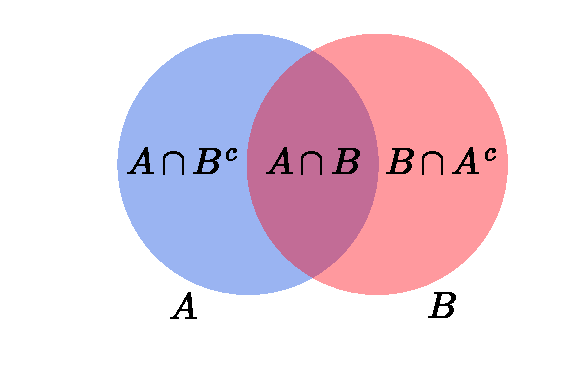
\includegraphics[width=\textwidth]{figuras/sets_union_probability.pdf}
  \end{minipage}\hfill
  \begin{minipage}[c]{0.53\textwidth}
    \caption{
       Diagrama de Venn con los eventos \(A\) y \(B\). Se observa que se cumple que \(A\cup B=AB^c\cup BA^c\cup AB\), donde los eventos  \(AB^c\), \(BA^c\) y \(AB\) son disjuntos. 
    } \label{fig:sets_union_probability}
  \end{minipage}
\end{figure}
\item \emph{Principio de inclusión-exclusión}: si \(A_1,\,\dots,\,A_n\) son eventos, se cumple que
\begingroup
\addtolength{\jot}{1em}
\begin{equation}\label{eq:inclusion_exclusion_principle}
 \begin{aligned}
 P\left(\bigcup_{i=1}^nA_i\right)&=\sum_{i=1}^nP(A_i)-\sum_{1\leq i_1 < i_2\leq n}P(A_{i_1}A_{i_2})+\sum_{1\leq i_1 < i_2 < i_3\leq n}P(A_{i_1}A_{i_2}A_{i_3})+\cdots\\
   &\qquad+(-1)^{n-1}\sum_{1\leq i_1 <\dots< i_{n-1}\leq n}P(A_{i_1}\cdots A_{i_{n-1}})+(-1)^nP(A_1\cdots A_n).
\end{aligned}
\end{equation}
\endgroup 
El principio puede demostrarse por inducción. Ya se demostró que se cumple para \(n=2\), dado por la ecuación \ref{eq:events_union}. Asumiendo que se cumple para \(n\), como en la ecuación \ref{eq:inclusion_exclusion_principle}, hay que demostrar que se cumple para \(n+1\). Desarrollando el lado izquierdo para \(n+1\), se tiene que
\begin{align}\label{eq:inclusion_exclusion_principle_tmp}
 P(A_1\cup\dots\cup A_n\cup A_{n+1})&\overset{(a)}{=}P[(A_1\cup\dots\cup A_n)\cup A_{n+1}]\nonumber\\
  &\overset{(b)}{=}P(A_1\cup\dots\cup A_n)+P(A_{n+1})-P[(A_1\cup\dots\cup A_n)\cap A_{n+1}]\nonumber\\
  &\overset{(c)}{=}P(A_1\cup\dots\cup A_n)+P(A_{n+1})-P[(A_1\cap A_{n+1})\cup\dots\cup(A_n\cap A_{n+1})],
\end{align}
donde en \((a)\) se empleó la propiedad asociativa de la operación de unión, en \((b)\) se empleó el principio de inclusión-exclusión para \(n=2\) y en \((c)\) la propiedad distributiva de la operación de intersección. El primer y tercer sumando consisten en probabilidades de \(n\) uniones, y por hipótesis se cumple el principio de inclusión-exclusión, que para el primer sumando está dado por la ecuación \ref{eq:inclusion_exclusion_principle} y para el tercer sumando es
\begingroup
\addtolength{\jot}{1em}
\begin{equation*}
 \begin{aligned}
 P\left(\bigcup_{i=1}^{n}A_{i}A_{n+1}\right)&=\sum_{i=1}^nP(A_iA_{n+1})-\sum_{1\leq i_1 < i_2\leq n}P(A_{i_1}A_{i_2}A_{n+1})+\cdots\\
   &\qquad+(-1)^{n-1}\sum_{1\leq i_1 <\dots< i_{n-1}\leq n}P(A_{i_1}\cdots A_{i_{n-1}}A_{n+1})+(-1)^nP(A_1\cdots A_nA_{n+1}).
\end{aligned}
\end{equation*}
\endgroup 
Sustituyendo esos resultados en la ecuación \ref{eq:inclusion_exclusion_principle_tmp}, se obtiene que
\begingroup
\addtolength{\jot}{1em}
\begin{equation*}
 \begin{aligned}
 P\left(\bigcup_{i=1}^{n+1}A_{i}\right)&=\Bigg[\sum_{i=1}^nP(A_i)-\sum_{1\leq i_1 < i_2\leq n}P(A_{i_1}A_{i_2})+\sum_{1\leq i_1 < i_2 < i_3\leq n}P(A_{i_1}A_{i_2}A_{i_3})+\cdots\\
   &\qquad+(-1)^nP(A_1\cdots A_n)\Bigg]\\
   &\qquad+ P(A_{n+1})\\
   &\qquad-\Bigg[\sum_{i=1}^nP(A_iA_{n+1})-\sum_{1\leq i_1 < i_2\leq n}P(A_{i_1}A_{i_2}A_{n+1})+\cdots\\
   &\qquad+(-1)^{n-1}\sum_{1\leq i_1 <\dots< i_{n-1}\leq n}P(A_{i_1}\cdots A_{i_{n-1}}A_{n+1})+(-1)^nP(A_1\cdots A_nA_{n+1})\Bigg].
\end{aligned}
\end{equation*}
\endgroup 
y reordenando los sumandos, la expresión puede escribirse como
\begingroup
\addtolength{\jot}{1em}
\begin{equation}\label{eq:inclusion_exclusion_principle_tmp1}
 \begin{aligned}
 P\left(\bigcup_{i=1}^{n+1}A_{i}\right)&=\left[\sum_{i=1}^nP(A_i)+ P(A_{n+1})\right]
 -\left[\sum_{1\leq i_1 < i_2\leq n}P(A_{i_1}A_{i_2})+\sum_{i=1}^nP(A_iA_{n+1})\right]\\
   &\qquad+\left[\sum_{1\leq i_1 < i_2 < i_3\leq n}P(A_{i_1}A_{i_2}A_{i_3})+\sum_{1\leq i_1 < i_2\leq n}P(A_{i_1}A_{i_2}A_{n+1})\right]+\cdots\\
   &\qquad+(-1)^n\left[P(A_1\cdots A_n)+\sum_{1\leq i_1 <\dots< i_{n-1}\leq n}P(A_{i_1}\cdots A_{i_{n-1}}A_{n+1})\right]\\
   &\qquad +(-1)^{n+1}P(A_1\cdots A_nA_{n+1}).
\end{aligned}
\end{equation}
\endgroup 
El paso siguiente, es notar que cada sumando entre paréntesis rectos puede agruparse en una sola sumatoria. Por ejemplo, los sumandos de la sumatoria en la penúltima expresión entre paréntesis rectos son las \(\binom{n}{n-1}=n\) probabilidades de los productos de los siguientes \(n\) factores
\[\arraycolsep=2pt\def\arraystretch{1.2}
\begin{array}{cccccccc}
  A_1&A_2&A_3&\cdots&A_{n-2}&A_{n-1}&\TikCircle&A_{n+1}\\
  A_1&A_2&A_3&\cdots&A_{n-2}&\TikCircle&A_n&A_{n+1}\\
  A_1&A_2&A_3&\cdots&\TikCircle&A_{n-1}&A_n&A_{n+1}\\
  \vdots& \vdots &\vdots & \iddots &\vdots& \vdots &\vdots &\vdots \\
  A_1& A_2 &\TikCircle&\cdots& A_{n-2}&A_{n-1}&A_n&A_{n+1}\\
  A_1&\TikCircle&A_3&\cdots&A_{n-2}&A_{n-1}&A_n&A_{n+1}\\
  \TikCircle & A_2 &A_3&\cdots&A_{n-2}&A_{n-1}&A_n&A_{n+1},
\end{array}
\]
y al sumar el término \(P(A_1\cdots A_n)\), se obtiene la suma de las \(n+1\) probabilidades de los productos de \(n\) factores
\[\arraycolsep=2pt\def\arraystretch{1.2}
\begin{array}{cccccccc}
  A_1&A_2&A_3&\cdots&A_{n-2}&A_{n-1}&A_n&\TikCircle\\
  A_1&A_2&A_3&\cdots&A_{n-2}&A_{n-1}&\TikCircle&A_{n+1}\\
  A_1&A_2&A_3&\cdots&A_{n-2}&\TikCircle&A_n&A_{n+1}\\
  A_1&A_2&A_3&\cdots&\TikCircle&A_{n-1}&A_n&A_{n+1}\\
  \vdots& \vdots &\vdots & \iddots &\vdots& \vdots &\vdots &\vdots \\
  A_1& A_2 &\TikCircle&\cdots& A_{n-2}&A_{n-1}&A_n&A_{n+1}\\
  A_1&\TikCircle&A_3&\cdots&A_{n-2}&A_{n-1}&A_n&A_{n+1}\\
  \TikCircle & A_2 &A_3&\cdots&A_{n-2}&A_{n-1}&A_n&A_{n+1},
\end{array}
\]
expresión que se puede escribir como
\[
 \sum_{1\leq i_1 <\dots< i_{n}\leq n+1}P(A_{i_1}\cdots A_{i_{n}}).
\]
Generalizando este razonamiento para todos los sumandos entre paréntesis rectos de la ecuación \ref{eq:inclusion_exclusion_principle_tmp1}, se obtiene que
\begingroup
\addtolength{\jot}{1em}
\begin{equation*}
 \begin{aligned}
 P\left(\bigcup_{i=1}^{n+1}A_{i}\right)&=\sum_{i=1}^{n+1}P(A_i)
   -\sum_{1\leq i_1 < i_2\leq n+1}P(A_{i_1}A_{i_2})
   +\sum_{1\leq i_1 < i_2 < i_3\leq n+1}P(A_{i_1}A_{i_2}A_{i_3})+\cdots\\
   &\qquad+(-1)^n\sum_{1\leq i_1 <\dots< i_{n}\leq n+1}P(A_{i_1}\cdots A_{i_{n}})\\
   &\qquad+(-1)^{n+1}P(A_1\cdots A_{n+1}),
\end{aligned}
\end{equation*}
\endgroup 
con lo que queda demostrado el paso inductivo.
\item \emph{Propiedad de monotonía}. La medida de probabilidad \(P\) es no decreciente: dados dos eventos \(A\) y \(B\), se cumple que
\begin{equation}\label{eq:probability_monotony_property}
 \textrm{si } A\subset B\qquad \Rightarrow\qquad P(A)\leq P(B).
\end{equation}
Efectivamente, como \(B=A\cup(B\setminus A)\) y los conjuntos \(A\) y \(B\setminus A\) son disjuntos, se cumple que
\[
 P(B)=P(A)+P(B\setminus A)\geq P(A).
\]
\item \emph{Desigualdad de Boole}. La medida de probabilidad \(P\) es contable sub-aditiva: para eventos cualesquiera \(A_n\), \(n\geq 1\), se cumple que
\begin{equation}\label{eq:boole_inequality}
 P\left(\bigcup_{n=1}^{\infty}A_n\right)\leq\sum_{n=1}^{\infty}P(A_n).
\end{equation}
Para demostrarlo, considérese la secuencia de eventos
\[
 B_1=A_1,\quad B_2=A_2\setminus A_1,\quad B_3=A_3\setminus(A_1\cup A_2),\dots,\quad B_n=A_n\setminus\left(\bigcup_{k=1}^{n-1}A_k\right),\dots
\]
Los eventos \(B_n\) son disjuntos, su unión es igual a la unión de los eventos \(A_n\) y además \(B_n\subseteq A_n\). Por lo tanto, se cumple que
\[
 P\left(\bigcup_{n=1}^{\infty}A_n\right)=P\left(\bigcup_{n=1}^{\infty}B_n\right)=\sum_{n=1}^{\infty}P(B_n)\leq \sum_{n=1}^{\infty}P(A_n).
\]
\end{enumerate}

\subsubsection{Espacios contables} 

Si el espacio muestral \(\Omega\) tiene un número finito \(N\) de resultados posibles, la probabilidad de todos los eventos puede ser expresada en términos de las probabilidades
\[
 P\{\zeta_i\}=p_i
\]
de los resultados elementales \(\{\zeta_i\}\). Debido a las propiedades de la medida de probabilidad, los valores \(p_i\) deben ser no-negativos y su suma debe valer 1,
\[
 p_i\geq 0,\qquad p_1+\dots+p_N=1.
\]
Considérese el caso en que el evento \(A\) consiste en \(r\) resultados elementales \(\zeta_{k_i}\), \(i=1,\dots,\,r\). Como \(A\) puede expresarse como la unión de los resultados elementales \(\{\zeta_{k_i}\}\), se cumple que
\[
 P(A)=P\{\zeta_{k_1}\}+\dots+P\{\zeta_{k_r}\}=p_{k_1}+\dots+p_{k_r}.
\]
Por la propiedad contable aditiva de la medida de probabilidad (ecuación \ref{eq:probability_measure_countably_additive}), esto también es cierto en el caso en que \(\Omega\) consiste en una cantidad infinita pero contable de resultados elementales. 

\paragraph{Ejemplo} El siguiente ejemplo (ejemplo 2.8 de \cite{papoulis2002probability}) muestra como es posible determinar las probabilidades de eventos complejos expresándolos como la unión de eventos mas simples mutuamente excluyentes.

Una urna contiene \(m\) bolas blancas y \(n\) bolas negras. Se extrae aleatoriamente una bola por vez sin reposición. Se quiere calcular la probabilidad de extraer alguna bola blanca antes de la \(k\)-ésima extracción (inclusive).

Denótese como \(W_k\) al evento
\[
 W_k=\{\textrm{una bola blaca es extraída antes de la }k\textrm{-ésima extracción}\}.
\]
Notar que el complemento del evento \(W_k\) es la extracción de \(k\) bolas negras en las \(k\) extracciones. El evento \(W_k\) puede ocurrir de las siguientes formas mutuamente excluyentes: se extre una bola blanca en la primera extracción, o se extrae una bola negra seguida de una bola blanca, o se extraen dos bolas negras seguidas de una bola blanca, y así sucesivamente hasta la extracción de \(k-1\) bolas negras seguida de una bola blanca.  Sea el evento
\[
 X_i=\{\textrm{se extraen }i\textrm{ bolas negras seguidas de una bola blanca}\},\qquad i=0,\,1,\dots,\,n.
\]
De esta forma,
\[
 W_k = X_0\cup X_1\cup.\dots\cup X_{k-1},
\]
y como los eventos \(X_i\) son mutuamente excluyentes, se cumple que
\[
 P(W_k)=\sum_{i=0}^{k-1}P(X_i).
\]
Observando que
\begin{align*}
 P(X_0)&=\frac{m}{m+n}\\
 P(X_1)&=\frac{n}{m+n}\cdot\frac{m}{m+n-1}\\
 P(X_2)&=\frac{n}{m+n}\cdot\frac{n-1}{m+n-1}\cdot\frac{m}{m+n-2}\\
 %P(X_3)&=\frac{n}{m+n}\cdot\frac{n-1}{m+n-1}\cdot\frac{n-2}{m+n-2}\cdot\frac{m}{m+n-3}\\
 \vdots \quad& \\
 P(X_i)&=\frac{n}{m+n}\cdot\frac{n-1}{m+n-1}\cdots\frac{n-(i-1)}{m+n-(i-1)}\cdot\frac{m}{m+n-i}\\
 \vdots \quad& \\
 P(X_{k-1})&=\frac{n}{m+n}\cdot\frac{n-1}{m+n-1}\cdots\frac{n-(k-2)}{m+n-(k-2)}\cdot\frac{m}{m+n-(k-1)},
\end{align*}
y sumando se obtiene que
\begin{equation}\label{eq:example_2-8_result}
 \begin{aligned}
 P(W_k) = \frac{m}{m+n}\bigg\{1&+\frac{n}{m+n-1}+\frac{n[n-1]}{[m+n-1][m+n-2]}+\cdots\\
  &+\frac{n[n-1]\cdots[n-(k-2)]}{[m+n-1][m+n-2]\cdots[m+n-(k-1)]}\bigg\},
\end{aligned}
\end{equation}
que es el resultado que se buscaba. 

Es interesante notar que en la extracción \(n+1\), se debe haber extraído al menos una bola blanca, por lo que
\[
 P(W_{n+1})=1.
\]
Sustituyendo este resultado en la ecuación \ref{eq:example_2-8_result}, es decir, evaluando en \(k=n+1\) e igualando a 1, se obtiene la siguiente interesante identidad:
\[
 1+\frac{n}{m+n-1}+\frac{n(n-1)}{(m+n-1)(m+n-2)}+\cdots+\frac{n(n-1)\cdots2\cdot1}{(m+n-1)(m+n-2)\cdots(m+1)m}=\frac{m+n}{m}.
\]

También vale la pena observar que, como se mencionó previamente, el evento
\[
 Y_k=\{\textrm{se extraen }k\textrm{ bolas negras en }k\textrm{ extracciones}\}
\]
es el complemento del evento \(W_k\), y por lo tanto,
\[
 P(W_k)=1-P(Y_k).
\]
Como \(Y_k\) ocurre cuando se extrae una bola negra en la primer extracción, y se extrae una bola negra en la segunda extracción y así sucesivamente hasta la \(k\)-ésima extracción, se tiene que
\[
 P(Y_k)=\frac{n}{m+n}\cdot\frac{n-1}{m+n-1}\cdots\frac{n-(k-1)}{m+n-(k-1)},
\]
y por lo tanto,
\[
 P(W_k)=1-\frac{n(n-1)\cdots(n-k+1)}{(n+m)(n+m-1)\cdots(n+m-k+1)}.
\]
Esta expresión es equivalente a la de la ecuación \ref{eq:example_2-8_result}.

\subsubsection{Espacios no contables. El eje real.}

Si el espacio muestral \(\Omega\) consiste en una cantidad infinita no contable de elementos, la probabilidad de los eventos no puede expresarse en función de la probabilidad de los resultados elementales.
Considérese que \(\Omega\) es el conjunto de todos los números reales. Sus subconjuntos son conjuntos arbitrarios de puntos en el eje real. Puede demostrarse que no es posible asignar probabilidades a todos los subconjuntos de \(\Omega\) de forma de satisfacer las propiedades de una medida de probabilidad. 

Para construir una medida de probabilidad sobre el eje real, se considerarán como eventos todos los intervalos \(x_1\leq x\leq x_2\), y sus uniones e intersecciones contables. Puede demostrarse que estos eventos forman un \(\sigma\)-álgebra de eventos. Este \(\sigma\)-álgebra incluye todas las semirectas \(x\leq x_i\), donde \(x_i\) es cualquier número real. También contiene todos los intervalos abiertos y cerrados, todos los puntos individuales del eje real, y en general, todos los conjuntos de puntos de interés práctico en las aplicaciones. Sin embargo, es posible demostrar que existen conjuntos de puntos en el eje real que no son uniones e intersecciones contables de intervalos, y por lo tanto, el \(\sigma\)-álgebra generado por intervalos no contiene todos los subconjuntos de \(\Omega\). 

Para obtener una especificación completa de un espacio de probabilidad sobre el eje real, alcanza con asignar probabilidades a los eventos \(\{x\leq x_i\}\). El resto de las probabilidades surgen de las propiedades de la medida de probabilidad. Supóngase que \(\alpha(x)\) es una función que cumple que
\[
 \int_{-\infty}^{\infty}\alpha(x)dx=1,\qquad \alpha(x)\geq 0.
\]
Se define la probabilidad del evento \(\{x\leq x_i\}\) como
\[
 P\{x\leq x_i\}=\int_{-\infty}^{x_i}\alpha(x)dx.
\]
De esta forma, quedan especificadas todas las probabilidades del espacio de probabilidad. Por ejemplo, para obtener la probabilidad del evento \(\{x_1<x\leq x_2\}\), se observa que
\[
 \{x\leq x_1\}\cup\{x_1<x\leq x_2\}=\{x\leq x_2\},
\]
donde los eventos \(\{x\leq x_1\}\) y \(\{x_1<x\leq x_2\}\) son mutuamente excluyentes. Por lo tanto, se cumple que
\[
 P\{x\leq x_1\}+P\{x_1<x\leq x_2\}=P\{x\leq x_2\}.
\]
De esta forma,
\begin{align*}
 P\{x_1<x\leq x_2\}&=P\{x\leq x_2\}-P\{x\leq x_1\}\\
   &=\int_{-\infty}^{x_2}\alpha(x)dx-\int_{-\infty}^{x_1}\alpha(x)dx\\
   &=\int_{x_1}^{x_2}\alpha(x)dx,
\end{align*}
quedando definida la probabilidad del evento \(\{x_1<x\leq x_2\}\) como
\begin{equation}\label{eq:interval_probability_real_line_space}
 P\{x_1<x\leq x_2\}=\int_{x_1}^{x_2}\alpha(x)dx.
\end{equation}
Se observa además que si la función \(\alpha(x)\) es acotada, la integral \ref{eq:interval_probability_real_line_space} tiende a 0 cuando \(x_1\to x_2\). Esto conduce a la conclusión de que la probabilidad del resultado elemental \(\{x_2\}\) es nula para todo \(x_2\) en el eje real. La probabilidad de cada resultado elemental de \(\Omega\) es 0, a pesar de que la probabilidad de su unión es 1. Esto no entra en conflicto con la propiedad contable aditiva de la medida de probabilidad dada por la ecuación \ref{eq:probability_measure_countably_additive}, ya que la cantidad de elementos de \(\Omega\) no es contable.

\subsection{Continuidad de la medida de probabilidad}\label{sec:probability_measure_continuity} 

Se presentan a continuación los teoremas vinculados a la \emph{continuidad} de la función de probabilidad. La medida de probabilidad es una función continua en el sentido de que si una secuencia de eventos \(\{A_n\}_{n=1}^{\infty}\) tiene límite, se cumple que \(P(\lim A_n)=\lim P(A_n)\). Se comenzará demostrando una versión mas liviana de este teorema para el caso particular de secuencias crecientes y decrecientes.

\paragraph{Teorema} \emph{Continuidad para secuencias crecientes}: sea \(\{A_n\}_{n=1}^{\infty}\) una secuencia creciente de eventos, entonces se cumple que
\[
 P\left(\lim_n A_n\right)=\lim_n P\left(A_n\right).
\]
Además, como \(P(A_n)\) es una función creciente, se cumple que
\[
 P(A_n)\nearrow\lim_n P(A_n).
\]
\paragraph{Demostración} Como se vio en la sección \ref{sec:monotone_sequences}, el limite de una secuencia creciente existe y está dado por
\[
 \lim_n A_n=\bigcup_{k=1}^{\infty}A_k.
\]
Notar que por ser una secuencia creciente, para cualquier \(n\) se cumple que
\[
 \bigcup_{k=1}^{n}A_k=A_n\qquad\Rightarrow\qquad P\left(\bigcup_{k=1}^{n}A_k\right)=P(A_n).
\]
Para demostrar el teorema, se define la secuencia de eventos disjuntos
\[
 B_1=A_1,\quad B_2=A_2\setminus A_1,\dots,\quad B_n=A_n\setminus A_{n-1},\dots
\]
Notar que se cumple que 
\[
 \bigcup_{k=1}^{n}B_k=\bigcup_{k=1}^{n}A_k=A_n,
\]
y por lo tanto,
\[
 \bigcup_{k=1}^{\infty}B_k=\bigcup_{k=1}^{\infty}A_k.
\]
De esta forma,
\begin{align*}
 P\left(\lim_n A_n\right)&=P\left(\bigcup_{k=1}^{\infty}A_k\right)\\
   &=P\left(\bigcup_{k=1}^{\infty}B_k\right)\\
   &\overset{(a)}{=}\sum_{k=1}^{\infty}P(B_k)\\
   &=\lim_n\sum_{k=1}^{n}P(B_k)\\
   &\overset{(b)}{=}\lim_n P\left(\bigcup_{k=1}^{n}B_k\right)\\
   &=\lim_n P(A_n),
\end{align*}
donde en \((a)\) y \((b)\) se empleó la propiedad contable aditiva de \(P\) para eventos disjuntos.

\paragraph{Teorema} \emph{Continuidad para secuencias decrecientes}: sea \(\{A_n\}_{n=1}^{\infty}\) una secuencia decreciente de eventos, entonces se cumple que
\[
 P\left(\lim_n A_n\right)=\lim_n P\left(A_n\right).
\]
Además, como \(P(A_n)\) es una función decreciente, se cumple que
\[
 P(A_n)\searrow\lim_n P(A_n).
\]
\paragraph{Demostración} Como la sucesión \(\{A_n\}_{n=1}^{\infty}\) es decreciente, la sucesión \(\{A_n^c\}_{n=1}^{\infty}\) es creciente. Por lo tanto,
\begin{align*}
 P\left(\lim_n A_n\right)&\overset{(a)}{=}P\left(\bigcap_{k=1}^{\infty}A_k\right)\\
   &\overset{(b)}{=}1-P\left[\left(\bigcap_{k=1}^{\infty}A_k\right)^c\right]\\
   &\overset{(c)}{=}1-P\left(\bigcup_{k=1}^{\infty}A_k^c\right)\\
   &\overset{(d)}{=}1-P\left(\lim_n A_n^c\right)\\
   &\overset{(e)}{=}1-\lim_n P\left(A_n^c\right)\\
   &\overset{(f)}{=}1-\lim_n\left[1-P(A_n)\right]\\
   &=\lim_n P(A_n),
\end{align*}
donde en \((a)\) se consideró que \(A_n\) es decreciente por lo que el límite existe y está dado por la ecuación \ref{eq:decreasing_sequence_limit}, en \((b)\) y en \((f)\) se empleó la propiedad \ref{complement_probability} de la medida de probabilidad, en \((c)\) se aplicaron leyes de Morgan, en \((d)\) se empleó que \(A_n^c\) es creciente y el límite está dado por la ecuación \ref{eq:increasing_sequence_limit}, y en \((e)\) se aplicó el resultado del teorema anterior de la continuidad de la función de probabilidad para secuencias crecientes.

\paragraph{Lema} \emph{Lema de Fatou}: sea \(\{A_n\}_{n=1}^{\infty}\) una secuencia arbitraria de eventos, entonces se cumple que
\begin{equation}\label{eq:fatou_lemma}
  P\left(\liminf_n A_n\right)\leq\liminf_n P\left(A_n\right).
\end{equation}
\paragraph{Demostración} Recordar que 
\[
 \liminf_n A_n = \bigcup_{n=1}^{\infty }\bigcap_{k=n}^{\infty }A_k = \bigcup_{n=1}^{\infty}G_n,
\]
donde se definió la secuencia creciente \(G_n=\bigcap_{k=n}^{\infty }A_k\), es el conjunto de resultados que ocurren ``eventualmente siempre''. Por lo tanto,
\begin{align}\label{eq:fatou_lemma_tmp}
 \lim_n P\left(G_n\right)&\overset{(a)}{=}P\left(\lim_n G_n\right)\nonumber\\
   &\overset{(b)}{=}P\left(\bigcup_{n=1}^{\infty } G_n\right)\nonumber\\
   &=P\left(\bigcup_{n=1}^{\infty } \bigcap_{k=n}^{\infty }A_k\right)\nonumber\\
   &=P\left(\liminf_n A_n\right),
\end{align}
donde en \((a)\) se empleó la continuidad de la función de probabilidad para secuencias crecientes y en \((b)\) se empleó que el límite de secuencias crecientes existe y está dado por la ecuación \ref{eq:increasing_sequence_limit}. Por otro lado, se tiene que como \(G_n=\bigcap_{k=n}^{\infty }A_k\), se cumple que
\[
 P(G_n)\leq \inf_{k\geq n} P(A_k),
\]
y tomando el límite cuando \(n\to\infty\), se tiene que
\[
 \lim_n P(G_n)\leq \lim_n\left[\inf_{k\geq n} P(A_k)\right].
\]
Como se vio previamente en la ecuación \ref{eq:fatou_lemma_tmp}, el lado izquierdo de la desigualdad converge a \(P\left(\liminf_n A_n\right)\), y el lado derecho converge a \(\liminf_n P(A_n)\), resultando en \ref{eq:fatou_lemma}, que es lo que se quería demostrar.

\paragraph{Lema} \emph{Lema de Fatou Reverso}: sea \(\{A_n\}_{n=1}^{\infty}\) una secuencia arbitraria de eventos, entonces se cumple que
\begin{equation}\label{eq:reverse_fatou_lemma}
  \limsup_n P\left(A_n\right)\leq P\left(\limsup_n A_n\right)
\end{equation}
\paragraph{Demostración} La demostración en análoga a la del lema de Fatou. Recordar que 
\[
 \limsup_n A_n = \bigcap_{n=1}^{\infty }\bigcup_{k=n}^{\infty }A_k = \bigcap_{n=1}^{\infty}G_n,
\]
donde se definió la secuencia decreciente \(G_n=\bigcup_{k=n}^{\infty }A_k\), es el conjunto de resultados que ocurren ``infinitamente a menudo''. Por un lado, se tiene que
\begin{align}\label{eq:reverse_fatou_lemma_tmp}
 \lim_n P\left(G_n\right)&\overset{(a)}{=}P\left(\lim_n G_n\right)\nonumber\\
   &\overset{(b)}{=}P\left(\bigcap_{n=1}^{\infty } G_n\right)\nonumber\\
   &=P\left(\bigcap_{n=1}^{\infty } \bigcup_{k=n}^{\infty }A_k\right)\nonumber\\
   &=P\left(\limsup_n A_n\right),
\end{align}
donde en \((a)\) se empleó la continuidad de la función de probabilidad para secuencias decrecientes y en \((b)\) se empleó que el límite de secuencias decrecientes existe y está dado por la ecuación \ref{eq:decreasing_sequence_limit}. Por otro lado, se tiene que como \(G_n=\bigcup_{k=n}^{\infty }A_k\), se cumple que
\[
 P(G_n)\geq \sup_{k\geq n} P(A_k),
\]
y tomando el límite cuando \(n\to\infty\), se tiene que
\[
 \lim_n P(G_n)\geq \lim_n\left[\sup_{k\geq n} P(A_k)\right].
\]
Como se vio previamente en la ecuación \ref{eq:reverse_fatou_lemma_tmp}, el lado izquierdo de la desigualdad converge a \(P\left(\limsup_n A_n\right)\), y el lado derecho converge a \(\limsup_n P(A_n)\), resultando en \ref{eq:reverse_fatou_lemma}, que es lo que se quería demostrar.

Es necesario realizar una consideración sobre los lemas de Fatou. En la ecuación \ref{eq:fatou_lemma} por ejemplo, el \(\liminf_n\) del lado izquierdo de la desigualdad se aplica sobre la secuencia de eventos \(A_n\), mientras que el \(\liminf_n\) del lado derecho se aplica sobre la sucesión de números \(P(A_n)\). Tanto el límite inferior \(\liminf_n\) como el límite superior \(\limsup_n\) aplicados a secuencias de eventos, fueron definidos en la sección \ref{sec:events_sequences_limit}. La definición del límite inferior y el límite superior aplicados a la sucesión de números \(x_n\) son las siguientes:
\[
 \liminf_{n\to\infty}x_n=\lim_{n\to\infty}\left(\inf_{k\geq n} x_k\right),\qquad
 \limsup_{n\to\infty}x_n=\lim_{n\to\infty}\left(\sup_{k\geq n} x_k\right),
\]
como ya se sugirió en la demostración de los lemas de Fatou. La interpretación de el límite inferior y el límite superior aplicado a sucesiones numéricas, se ilustra en la figura \ref{fig:liminf_limsup}\footnote{Fuente: \url{https://en.wikipedia.org/wiki/Limit_superior_and_limit_inferior}}.
\begin{figure}[!htb]
\begin{center}
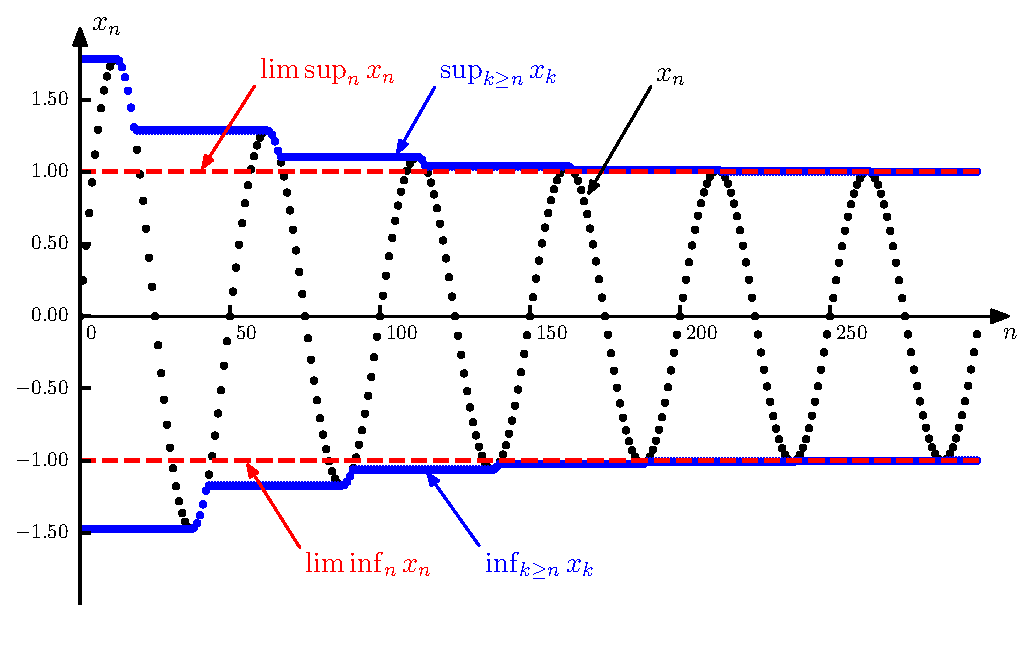
\includegraphics[width=0.8\columnwidth]{figuras/liminf_limsup.pdf}
\caption{\label{fig:liminf_limsup} Ilustración del límite inferior y el límite superior aplicado a la secuencia de números \(x_n\). La secuencia \(x_n\) se grafica en negro. La secuencia \(\sup_{k\geq n} x_k\) es una secuencia en \(n\), donde el valor que toma en \(n\) se obtiene como el máximo valor que toma \(x_k\) en \(k\geq n\). El límite superior \(\limsup_n x_n\) es el límite de la secuencia \(\sup_{k\geq n} x_k\) cuando \(n\to\infty\). Análogamente, \(\inf_{k\geq n} x_k\) es la secuencia que consiste en el mínimo de \(x_k\) para \(k\geq n\) para cada valor de \(n\), y el límite inferior \(\liminf_n x_n\) es el límite de dicha secuencia cuando \(n\to\infty\). El límite inferior y el límite superior coinciden si y solo si la secuencia converge.}
\end{center}
\end{figure}

Combinando el lema de Fatou y el lema de Fatou reverso, se obtienen las siguientes desigualdades:
\begin{equation}\label{eq:fatou_inequalities}
 P\left(\liminf_n A_n\right)\leq\liminf_n P\left(A_n\right)\leq\limsup_n P\left(A_n\right)\leq P\left(\limsup_n A_n\right),
\end{equation}
donde la primera y ultima desigualdad son el lema de Fatou y el lema de Fatou reverso respectivamente, y la desigualdad del centro proviene de que para cualquier secuencia numérica \(x_n\), se cumple que
\[
 \inf_{k\geq n}x_k\leq\sup_{k\geq n}x_k,\qquad\textrm{para todo }n. 
\]
\paragraph{Ejemplo} Sea \(\Omega=\{0,\,1\}\), con medida de probabilidad \(P(\{0\})=1/3\) y \(P(\{1\})=2/3\). El \(\sigma\)-álgebra de eventos es en este caso \(\mathcal{F}=\{\emptyset,\,\{0\},\,\{1\},\,\Omega\}\) con probabilidades 0, 1/3, 2/3 y 1 respectivamente. Sea la secuencia de eventos
\[
 A_n=
 \left\{\begin{array}{ll}
  \{0\}, & \textrm{si }n\textrm{ es par} \\
  \{1\}, & \textrm{si }n\textrm{ es impar}
 \end{array} \right..
\]
Se calculará \(P(\liminf_n A_n)\), \(P(\limsup_n A_n)\), \(\liminf_n P(A_n)\) y \(\limsup_n P(A_n)\). Considerando que 
\[
 \bigcup_{k=n}^{\infty }A_k=\{0,\,1\},\qquad \bigcap_{k=n}^{\infty}A_k=\emptyset,\qquad \forall n,
\]
se tiene que
\[
 \limsup_n A_n=\bigcap_{n=1}^{\infty}\bigcup_{k=n}^{\infty}A_k=\bigcap_{n=1}^{\infty}\{0,\,1\}=\{0,\,1\}=\Omega,
\]
y
\[
 \liminf_n A_n=\bigcup_{n=1}^{\infty}\bigcap_{k=n}^{\infty}A_k=\bigcup_{n=1}^{\infty}\emptyset=\emptyset.
\]
Por lo tanto,
\[
 P\left(\limsup_{n\rightarrow \infty }A_n\right)=1,\qquad P\left(\liminf_{n\rightarrow \infty }A_n\right)=0.
\]
Además, como
\[
 \sup_{k\geq n}P(A_k)=\frac{2}{3},\qquad \inf_{k\geq n}P(A_k)=\frac{1}{3},\qquad\forall n
\]
se tiene que
\[
 \limsup_n P(A_n)=\frac{2}{3},\qquad \liminf_n P(A_n)=\frac{1}{3}.
\]
Notar que se cumplen las desigualdades de los lemas de Fatou dadas por la ecuación \ref{eq:fatou_inequalities}.

\paragraph{Teorema} \emph{Continuidad de la medida de probabilidad}: si una secuencia de eventos \(\{A_n\}_{n=1}^{\infty}\) tiene límite, entonces se cumple que
\begin{equation}\label{eq:probability_continuity}
  P\left(\lim_n A_n\right) = \lim_n P\left(A_n\right).
\end{equation}
\paragraph{Demostración} Como la secuencia tiene límite, se cumple que (ver sección \ref{sec:events_sequences_limit})
\[
 \lim_n A_n=\limsup_n A_n=\liminf_n A_n
\]
y por lo tanto, 
\[
 P\left(\lim_n A_n\right)=P\left(\limsup_n A_n\right)=P\left(\liminf_n A_n\right).
\]
Esto indica que las desigualdades de los lemas de Fatou de la ecuación \ref{eq:fatou_inequalities} deben ser igualdades, y por lo tanto
\[
 \limsup_n P(A_n)=\liminf_n P(A_n)=\lim_n P(A_n),
\]
concluyendo la prueba.

Se presenta a continuación el lema de Borel-Cantelli, que es la herramienta básica para demostrar convergencia casi segura.

\paragraph{Lema} \emph{Lema de Borel-Cantelli}: sea \(\{A_n\}_{n=1}^{\infty}\) una secuencia  de eventos tal que
\[
 \sum_n P(A_n)<\infty.
\]
Entonces, se cumple que
\[
  P\left(\limsup_n A_n\right) = P(\{A_n\,i.o.\})=0.
\]
Esto significa que el conjunto de elementos \(\omega\) del espacio muestral \(\Omega\) que pertenecen a una cantidad infinita de eventos \(A_1,\,A_2,\dots\) tiene probabilidad 0 en \(\Omega\).

\paragraph{Demostración} Se define la secuencia decreciente
\[
 G_n=\bigcup_{k=n}^\infty A_k.
\]
Se cumple que
\[
 P(G_n)\searrow P\left(\limsup_n A_n\right),
\]
ya que
\[
 \lim_n P(G_n)\overset{(a)}{=}P\left(\lim_n G_n\right)
 \overset{(b)}{=}P\left(\bigcap_{n=1}^\infty G_n\right)
 =P\left(\bigcap_{n=1}^\infty \bigcup_{k=n}^\infty A_k\right)
 =P\left(\limsup_n A_n\right),
\]
donde en \((a)\) se empleó la continuidad de la medida de probabilidad para secuencias decrecientes y en \((b)\) que el límite de una secuencia decreciente existe y está dado por la ecuación \ref{eq:decreasing_sequence_limit}. Por lo tanto, para todo \(m\) se cumple que
\[
 P\left(\limsup_n A_n\right)\leq P(G_m)=P\left(\bigcup_{k=m}^\infty A_k\right)\leq\sum_{k=m}^\infty P(A_k)
\]
donde la última desigualdad proviene de la propiedad de sub-aditividad de la medida de probabilidad dada por la ecuación \ref{eq:boole_inequality}. Tomando \(m\to\infty\) y considerando que el lado derecho es la cola de una serie convergente y por lo tanto
\[
 \lim_{m\to\infty}\sum_{k=m}^\infty P(A_k)=0,
\]
se concluye la prueba.

\paragraph{Ejemplo} \emph{Paradoja de Ross–Littlewood} \cite{ross2009first9th}: supongase que se dispone de una urna infinitamente grande y una colección de infinitas bolillas etiquetadas con los números 1, 2, 3, etcétera. Considérese que se realiza el siguiente experimento: al minuto 1 antes del mediodía, las bolillas numeradas del 1 al 10 se introducen en la urna, y la bolilla de número 10 se extrae (asúmase que la extracción consume tiempo 0). Luego, a 1/2 minuto antes del mediodía, se introducen las bolillas numeradas del 11 al 20 y se extrae la bolilla 20. A 1/4 de minuto antes del mediodía, se introducen las bolillas numeradas del 21 al 30 y se extrae la bolilla 30, y así sucesivamente. 
Los tiempos en donde se ejecuta cada paso son así definidos para asegurar que una cantidad contable infinita de pasos se ejecutaron al mediodía. Una secuencia contable infinita de operaciones que se realizan en un tiempo finito se denomina \emph{supertarea}. 
La pregunta de interés es cuantas bolillas hay en la urna al mediodía.  

La respuesta a la pregunta claramente es que hay infinitas bolillas en la urna al mediodía, ya que toda bolilla cuyo número no sea de la forma \(10n\), para todo \(n\geq 1\), permanece en la urna.

Supóngase que ahora se modifica el experimento de la siguiente forma: al minuto 1 antes del mediodía, las bolillas numeradas del 1 al 10 se introducen en la urna, y la bolilla de número 1 se extrae. Luego, a 1/2 minuto antes del mediodía, se introducen las bolillas numeradas del 11 al 20 y se extrae la bolilla 2. A 1/4 de minuto antes del mediodía, se introducen las bolillas numeradas del 21 al 30 y se extrae la bolilla 3, y así sucesivamente. En este nuevo experimento, ¿cuantas bolillas hay en la urna al mediodía?

Tal vez sorprendentemente, la respuesta ahora es que la urna está vacía al mediodía. Efectivamente, considérese cualquier bolilla, la \(n\)-ésima por ejemplo. En algún momento previo al mediodía, esta bolilla será extraída. Concretamente, la bolilla \(n\) será extraída \((1/2)^{n-1}\) minutos antes del mediodía. Se concluye que para cada \(n\), la bolilla \(n\) no estará en la urna al mediodía, y por lo tanto, la urna estará vacía a esa hora.

Como se ve, la diferencia de los resultados de los experimentos proviene de la forma en que se extraen las bolillas. Se considera a continuación el caso en que cuando se extrae una bolilla, se hace de forma aleatoria entre las bolillas presentes en la urna. Es decir, 1 minuto antes del mediodía, se introducen las  bolillas numeradas del 1 al 10 y se extrae un bolilla al azar, y así sucesivamente. En este caso, ¿cuantas bolillas hay en la urna al mediodía?

Considérese la bolilla etiquetada con el número 1, y defínase \(E_n\) al evento que consiste en que la bolilla 1 está aún en la urna luego de \(n\) extracciones. Se comenzará calculando \(P(E_n)\). Para esto, se define \(A_n\) como el evento que consiste que no se extrae la bolilla 1 en el paso \(n\). De esta forma,
\[
 E_n=A_1\cap A_2\cap\dots\cap A_n,
\]
y como los eventos \(A_k\) son independientes (este concepto se verá mas adelante en el capítulo \ref{ch:repeated_trials}), se cumple que
\[
 P(E_n)=P(A_1)\times P(A_2)\times\dots\times P(A_n)=\prod_{k=1}^nP(A_k).
\]
Para calcular \(P(A_k)\), se observa que en el paso \(k\)-ésimo luego de insertar las 10 bolillas y previo a la extracción hay \(10k-(k-1)=9k+1\) bolillas en la urna, ya que se insertaron 10 bolillas en cada paso hasta el paso \(k\)-ésimo y se sacó una en los \(k-1\) pasos previos. De esas \(9k+1\) bolillas, \(9k\) no son la bolilla 1. Por lo tanto, la probabilidad de no extraer la bolilla en el paso \(k\) es
\[
 P(A_k)=\frac{9k}{9k+1},
\]
y por lo tanto,
\[
 P(E_n)=\prod_{k=1}^n\frac{9k}{9k+1}.
\]
Si bien los conceptos para llegar a este resultado no se han desarrollado aún en estos apuntes, el mismo puede deducirse con técnicas simple de conteo y la noción frecuentista de la probabilidad.

Ahora, la probabilidad de que la bolilla 1 está aún en la urna al mediodía es
\[
 P\{\textrm{bolilla 1 está en la urna al mediodía}\}=P\left(\lim_{n\to\infty} E_n\right).
\]
Para continuar con el razonamiento es necesario notar que la secuencia de eventos \(E_n\) es decreciente. Efectivamente, que la bolilla 1 esté en la urna en el paso \(n+1\) implica que esté en la urna en el paso \(n\), y por lo tanto,
\[
 E_{n+1}\subset E_n,\qquad \forall n\geq 1.
\]
De esta forma,
\begin{align*}
 P\{\textrm{bolilla 1 está en la urna al mediodía}\}&=P\left(\lim_{n\to\infty} E_n\right)\\
  &\overset{(a)}{=}\lim_{n\to\infty} P\left(E_n\right)\\
  &=\lim_{n\to\infty}\prod_{k=1}^n\frac{9k}{9k+1}\\
  &=\lim_{n\to\infty}\left[\prod_{k=1}^n\frac{9k+1}{9k}\right]^{-1}\\
  &=\lim_{n\to\infty}\left[\prod_{k=1}^n\left(1+\frac{1}{9k}\right)\right]^{-1},
\end{align*}
donde en \((a)\) se empleó la continuidad de la medida de probabilidad para secuencias de eventos decrecientes. Notando que para todo \(n\geq1\) se cumple que
\[
 \prod_{k=1}^n\left(1+\frac{1}{9k}\right)=\left(1+\frac{1}{9}\right)\left(1+\frac{1}{18}\right)\cdots\left(1+\frac{1}{9n}\right)>\frac{1}{9}+\frac{1}{18}+\cdots+\frac{1}{9n}=\sum_{k=1}^{n}\frac{1}{9k}
\]
se obtiene que
\[
 \left[\prod_{k=1}^n\left(1+\frac{1}{9k}\right)\right]^{-1}<\left[\frac{1}{9}\sum_{k=1}^{n}\frac{1}{k}\right]^{-1}.
\]
Tomando el límite con \(n\to\infty\), se tiene que
\[
 \lim_{n\to\infty}\left[\prod_{k=1}^n\left(1+\frac{1}{9k}\right)\right]^{-1}<\lim_{n\to\infty}\left[\frac{1}{9}\sum_{k=1}^{n}\frac{1}{k}\right]^{-1}=0
\]
ya que \(\sum_{k=1}^{\infty}1/k\) es la serie armónica y por lo tanto, diverge. Se concluye que
\[
 P\{\textrm{bolilla 1 está en la urna al mediodía}\}=0,
\]
es decir, la probabilidad de la bolilla 1 esté en la urna luego de infinitos pasos es 0.

Defínase a \(F_i\) como el evento de que la bolilla número \(i\) esté en la urna al mediodía. Se acaba de demostrar que \(P(F_1)=0\). De forma análoga se puede demostrar que \(P(F_i)=0\) para todo \(i\). Por ejemplo, puede verse que
\[
 P(F_i)=\lim_{n\to\infty}\prod_{k=2}^n\frac{9k}{9k+1},\qquad\textrm{para }i=11,\,12,\dots,\,20,
\]
y mas en general, se tiene que
\[
 P(F_i)=\lim_{n\to\infty}\prod_{k=m}^n\frac{9k}{9k+1},\qquad\textrm{para }i=10m-9,\dots,\,10m-1,\,10m.
\]
El rango de \(i\) corresponde a la numeración de las bolillas introducidas en el paso \(m\). A partir de esta expresión y siguiendo el mismo razonamiento que para \(F_1\), se obtiene que \(P(F_i)=0\) para todo \(i\).

Finalmente, la probabilidad que la urna no esté vacía al mediodía es
\[
 P\left(\bigcup_{i=1}^{\infty}F_i\right)\leq\sum_{i=1}^{\infty}P(F_i)=0,
\]
donde se empleó la desigualdad de Boole (ecuación \ref{eq:boole_inequality}). Por lo tanto, la urna estará vacía al mediodía con probabilidad 1.

\subsection{Probabilidad condicional}\label{sec:conditional_probability_events}

La probabilidad condicional de un evento \(A\) asumiendo la ocurrencia de otro evento \(M\) se define como
\begin{equation}\label{eq:conditional_probability_definition}
 P(A|M)={\frac{P(AM)}{P(M)}},
\end{equation}
donde se asume que \(P(M)\neq 0\). Es referida como ``la probabilidad de \(A\) dado \(M\)''.

Se puede demostrar que para un evento \(M\) específico, la probabilidad condicional \(P(A|M)\) es efectivamente una probabilidad, ya que cumple todas las propiedades de una medida de probabilidad. De esta forma, todos los resultados que involucran probabilidades se cumplen también para probabilidades condicionales.

\paragraph{Probabilidad total y el teorema de Bayes}

En el capítulo 2 de \cite{papoulis2002probability} se demuestra el teorema de la \emph{probabilidad total}, que indica que si \(U=[A_1,\,A_2,\,\dots,\,A_n]\) es una partición de \(S\) y \(B\) un evento arbitrario, se cumple que
\begin{equation}\label{eq:total_probability_theorem}
 P(B)=P(B|A_1)P(A_1)+P(B|A_2)P(A_2)+\cdots+P(B|A_n)P(A_n).
\end{equation}
Además, de \ref{eq:conditional_probability_definition} se tiene que
\[
  P(BA_i)=P(A_i|B)P(B)=P(B|A_i)P(A_i)
\]
y por lo tanto
\begin{equation}\label{eq:bayes_theorem_for_events_2}
 P(A_i|B)=\frac{P(B|A_i)P(A_i)}{P(B)}.
\end{equation}
Sustituyendo la ecuación \ref{eq:total_probability_theorem} en este último resultado, se obtiene el \emph{teorema de Bayes},
\begin{equation}\label{eq:bayes_theorem_for_events}
 P(A_i|B)=\frac{P(B|A_i)P(A_i)}{P(B|A_1)P(A_1)+\cdots+P(B|A_n)P(A_n)}.
\end{equation}
Usualmente se emplean los términos \emph{a priori} y \emph{a posteriori} para referirse a las probabilidades \(P(A_i)\) y \(P(A_i|B)\) respectivamente.

\subsection{Eventos independientes}\label{sec:independents_events}

Se dice que los eventos \(A\) y \(B\) son \emph{independientes} si se cumple que
\begin{equation}\label{eq:independent_events_definition}
 P(AB)=P(A)P(B).
\end{equation}

Se puede demostrar que si los eventos \(A\) y \(B\) son independientes, los eventos \(\bar{A}\) y \(B\) y los eventos \(\bar{A}\) y \(\bar{B}\) también son independientes.

\paragraph{Lema} \emph{Segundo lema de Borel-Cantelli}: sea \(\{A_n\}_{n=1}^{\infty}\) una secuencia de eventos \emph{mutuamente independientes} tal que
\[
 \sum_n P(A_n)=\infty.
\]
Entonces, se cumple que
\[
  P\left(\limsup_n A_n\right) = P(\{A_n\,i.o.\})=1.
\]
Esto significa que si la suma de las probabilidades de una secuencia infinita de eventos independientes diverge, el conjunto de elementos \(\omega\) del espacio muestral \(\Omega\) que pertenece a infinitos eventos \(A_1,\,A_2,\dots\) tiene probabilidad 1 en \(\Omega\), o equivalentemente, el evento \(\left\{\omega\in\Omega:\omega\in A_n\;i.o.\right\}\) ocurre \emph{casi seguramente} (ver sección \ref{sec:convergence_modes}).

\paragraph{Demostración} Se parte observando que
\begin{align*}
  \left(\limsup_{n\rightarrow\infty}A_n\right)^c&=\left(\bigcap_{n=1}^{\infty }\bigcup_{k=n}^{\infty }A_k\right)^c=\bigcup_{n=1}^{\infty}\left(\bigcup_{k=n}^{\infty}A_k\right)^c=\bigcup_{n=1}^{\infty}\bigcap_{k=n}^{\infty}A_k^c,
 \end{align*}
donde las identidades provienen de aplicar las leyes de Morgan. Por lo tanto, se cumple que
\begin{align}\label{eq:second_borel_tmp}
 P\left[\left(\limsup_{n\rightarrow\infty}A_n\right)^c\right]&=P\left(\bigcup_{n=1}^{\infty}\bigcap_{k=n}^{\infty}A_k^c\right)\nonumber \\ 
  &\leq \sum_{n=1}^{\infty}P\left(\bigcap_{k=n}^{\infty}A_k^c\right),
\end{align}
donde se empleó la desigualdad de Boole, dada por la ecuación \ref{eq:boole_inequality}.
Además, como los eventos de la secuencia \(\{A_n\}_{n=1}^{\infty}\) son mutuamente independientes, los eventos de la secuencia complementaria \(\{A_n^c\}_{n=1}^{\infty}\) también son mutuamente independientes, y por lo tanto
\begin{align*}
 P\left(\bigcap_{k=n}^{\infty}A_k^c\right)&=\prod_{k=n}^{\infty}P\left(A_k^c\right)\\
  &=\prod_{k=n}^{\infty}\left[1-P\left(A_k\right)\right]\\
  &\overset{(a)}{\leq}\prod_{k=n}^{\infty}e^{-P\left(A_k\right)}\\
  &=\exp\left[-\sum_{k=n}^{\infty}P\left(A_k\right)\right]\\
  &\overset{(b)}{=}0,
\end{align*}
donde en \((a)\) se empleó que \(1-x\leq e^{-x}\) para todo \(x\) y en \((b)\) la hipótesis \(\sum_n P(A_n)=\infty\). Combinando este resultado con el de la ecuación \ref{eq:second_borel_tmp}, se obtiene que
\[
 P\left[\left(\limsup_{n\rightarrow\infty}A_n\right)^c\right]\leq \sum_{n=1}^{\infty}P\left(\bigcap_{k=n}^{\infty}A_k^c\right)=0.
\]
y por lo tanto,
\[
 P\left(\limsup_{n\rightarrow\infty}A_n\right)=1.
\]

\paragraph{Ejemplo} Un ensayo de Bernoulli consiste en la repetición de un experimento que tiene los dos resultados posibles \(h\) y \(t\), con \(P\{h\}=p\) y \(P\{t\}=1-p\), como se explica mas detalladamente en la sección \ref{sec:bernoulli_trials}. El resultado de cada experimento es independiente del resultado de los demás experimentos. Un ejemplo de ensayo de Bernoulli, es lanzar al aire  una moneda repetidamente. 

Considérese el evento ``\(hh\cdots h\)'' en un ensayo de Bernoulli.
Se quiere determinar la probabilidad de que dicha secuencia de \(n\) resultados \(h\) sucesivos ocurra infinitamente a menudo. Para hacerlo, se considera el evento \(A_k=\{\)el resultado en el \(k\)-ésimo experimento es \(h\}\), y se define el evento \(B_i\) como
\[
 B_i=A_i\cap A_{i+1}\cap \cdots \cap A_{i+n-1},\qquad i\geq 1,
\]
que es la ocurrencia de \(n\) resultados \(h\) sucesivos entre el experimento \(i\)-ésimo y el experimento \(i+n-1\). Puede demostrarse (ver sección \ref{sec:bernoulli_trials}) que \(P(B_i)=p^n\). Los eventos \(B_i\) no son independientes, pero los eventos \(B_1,\,B_{n+1},\,B_{2n+1},\dots\) son independientes, y además
\[
 \sum_{k=0}^{\infty}P(B_{kn+1})=\sum_{k=0}^{\infty}p^n=\infty.
\]
Por lo tanto, por el segundo lema de Borel-Cantelli, el patrón ``\(hh\cdots h\)'', así como cualquier otro patrón arbitrario, ocurrira infinitamente a menudo con probabilidad 1.


\chapter{Ensayos repetidos}\label{ch:repeated_trials}

Se incluyen en este capítulo algunos conceptos desarrollados en el capítulo 3 de \cite{papoulis2002probability}.


\section{Experimentos combinados}

Se consideran dos experimentos. El primero consiste en tirar un dado,
\[
 S_1=\{f_1,\,\dots,\,f_6\}\qquad\qquad P_1\{f_i\}=\frac{1}{6},
\]
y el segundo en lanzar una moneda,
\[
 S_2=\{h,\,t\}\qquad\qquad P_2\{h\}=P_2\{t\}=\frac{1}{2}.
\]
Se realizan los dos experimentos y se quiere encontrar la probabilidad de obtener ``dos'' (\(f_2\)) en el dado y ``cara'' (\(h\)) en la moneda. Si se asume la hipótesis razonable de que el resultado del primer experimento es independiente del segundo experimento, según la ecuación \ref{eq:independent_events_definition} esta probabilidad es \(1/6\times1/2\). Sin embargo, en la definición de la ecuación \ref{eq:independent_events_definition} se asume que \(A\) y \(B\) son subconjuntos del mismo espacio muestral. Por lo tanto, para adaptar esta conclusión al caso del ejemplo considerado, hay que construir un espacio muestral \(S\) que contenga como subconjuntos los eventos ``dos'' y ``cara''. Esto se explica a continuación.

Ambos experimentos son vistos como un único experimento cuyas salidas son pares \(\zeta_1\zeta_2\), donde \(\zeta_1\) es una de las seis caras del dado y \(\zeta_2\) es uno de los dos resultados de la moneda. De esta forma, el espacio muestral \(S\) del experimento contiene 12 elementos,
\[
 S=\{f_1h,\dots,\,f_6h,\,f_1t,\dots,\,f_6t\}.
\]
En este espacio, \{dos\} no es un evento elemental, si no un subconjunto que contiene dos elementos,
\[
 \{\textrm{dos}\}=\{f_2h,\,f_2t\}.
\]
Análogamente, \{cara\} es un evento con seis elementos,
\[
 \{\textrm{cara}\}=\{f_1h,\dots,\,f_6h\}.
\]
Para especificar completamente al experimento, hay que asignar probabilidades a todos los subconjuntos de \(S\). Como el evento \{dos\} ocurre si en el dado sale ``dos'' independientemente del resultado de la moneda,
\[
 P\{\textrm{dos}\}=\frac{1}{6}.
\]
De igual forma, el evento \{cara\} ocurre si sale ``cara'' en la moneda sin importar el resultado del dado, y por lo tanto
\[
 P\{\textrm{cara}\}=\frac{1}{2}.
\]
Además, el evento \{dos\} es un resultado del primer experimento y el evento \{cara\} es resultado del segundo experimento, y por lo tanto es razonable asumirlos eventos independientes en el experimento combinado. La intersección de los eventos \{dos\} y \{cara\} es el evento elemental \(\{f_2h\}\) de \(S\). 
Por lo tanto, se aplica la ecuación \ref{eq:independent_events_definition} y se concluye que
\[
 P\{f_2h\}=P\{\textrm{dos}\}\times P\{\textrm{cara}\}=\frac{1}{6}\times\frac{1}{2}=\frac{1}{12}.
\]

\subsection{Producto cartesiano de conjuntos} 

Sean dos conjuntos \(S_1\) y \(S_2\) con elementos \(\zeta_1\) y \(\zeta_2\) respectivamente. El \emph{producto cartesiano} de los conjuntos \(S_1\) y \(S_2\) es un conjunto \(S\) cuyos elementos son todos los pares ordenados \(\zeta_1\zeta_2\), donde \(\zeta_1\) es cualquier elemento de \(S_1\) y  \(\zeta_2\) es cualquier elemento de \(S_2\). Se denota como
\[
 S=S_1\times S_2.
\]
Si \(A\) es un subconjunto de \(S_1\) y \(B\) es un subconjunto de \(S_2\), el conjunto
\[
 C=A\times B,
\]
que consiste en todos los pares \(\zeta_1\zeta_2\), con  \(\zeta_1\in A\) y \(\zeta_2\in B\), es un subconjunto de \(S\). Considérense los conjuntos \(A\times S_2\) y \(S_1\times B\). Claramente su intersección es el conjunto \(A\times B\),
\begin{equation}\label{eq:set_intersection_AB}
 A\times B=(A\times S_2)\cap(S_1\times B).
\end{equation}

\paragraph{Ejemplo} Supóngase que \(S_1\) es el eje \(x\), \(S_2\) es el eje \(y\), y \(A\) y \(B\) son los intervalos
\[
 A=\{x_1\leq x\leq x_2\},\qquad b=\{y_1\leq y\leq y_2\},
\]
como se muestra en la figura \ref{fig:set_intersection_axis_xy}. En ese caso, \(A\times S_2\) es una banda vertical, \(S_1\times B\) es una banda horizontal, y \(A\times B\) es un rectángulo.
\begin{figure}[!htb]
  \begin{minipage}[c]{0.4\textwidth}
    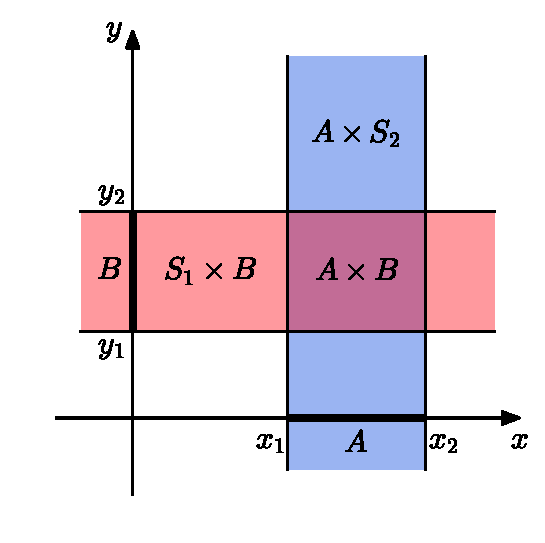
\includegraphics[width=\textwidth]{figuras/set_intersection_axis_xy.pdf}
  \end{minipage}\hfill
  \begin{minipage}[c]{0.5\textwidth}
    \caption{
       Conjuntos \(A\times S_2\), \(S_1\times B\) y \(A\times B\) cuando \(S_1\) es el eje \(x\), \(S_2\) es el eje \(y\) y \(A\) y \(B\) son intervalos en el eje \(x\) e \(y\) respectivamente.
    } \label{fig:set_intersection_axis_xy}
  \end{minipage}
\end{figure}

\subsection{Producto cartesiano de dos experimentos}

El producto cartesiano de dos experimentos \(S_1\) y \(S_2\) es un nuevo experimento \(S=S_1\times S_2\) cuyos eventos son todos los productos cartesianos de la forma 
\[
 A\times B,
\]
donde \(A\) es un evento de \(S_1\) y \(B\) es un evento de \(S_2\), y sus uniones y sus intersecciones. En este experimento las probabilidades de los eventos \(A\times S_2\) y \(S_1\times B\) son
\begin{equation}\label{eq:combined_experiments_intersection}
 P(A\times S_2)=P_1(A),\qquad P(S_1\times B)=P_2(B),
\end{equation}
donde \(P_1(A)\) es la probabilidad del evento \(A\) en el experimento \(S_1\) y \(P_2(B)\) es la probabilidad del evento \(B\) en el experimento \(S_2\). Efectivamente, el evento \(A\times S_1\) del experimento \(S\) ocurre si el evento \(A\) del experimento \(S_1\) ocurre sin importar el resultado del experimento \(S_2\). De la misma forma, el evento \(S_1\times B\) del experimento \(S\) ocurre si el evento \(B\) del experimento \(S_2\) ocurre sin importar el resultado del experimento \(S_1\).

La ecuación \ref{eq:combined_experiments_intersection} determina únicamente la probabilidad de los eventos y \(A\times S_2\) y \(S_1\times B\). La probabilidad de un evento arbitrario de la forma \(A\times B\) y la de sus uniones e intersecciones no pueden en general expresarse en función de \(P_1\) y \(P_2\). Para determinar estas probabilidad, se necesita mas información de los experimentos \(S_1\) y \(S_2\).

\subsubsection{Experimentos independientes}

En muchas aplicaciones, los eventos \(A\times S_2\) y \(S_1\times B\) del experimento combinado son independientes para cualquier \(A\) y \(B\). Como la intersección de esos eventos es \(A\times B\), se tiene que
\[
 P(A\times B)\overset{(a)}{=}P((A\times S_2)\cap(B\times S_1))\overset{(b)}{=}P(A\times S_2)P(S_1\times B)\overset{(c)}{=}P_1(A)P_2(B),
\]
donde en \((a)\) se empleó la ecuación \ref{eq:set_intersection_AB}, en \((b)\) se empleó la ecuación \ref{eq:independent_events_definition} y en \((c)\) la ecuación \ref{eq:combined_experiments_intersection}. Esto completa la especificación del experimento \(S\) en el caso en que los experimentos \(S_1\) y \(S_2\) son independientes, ya que todos los eventos de \(S\) son uniones e intersecciones de eventos de la forma \(A\times B\).

Notar que en particular el evento elemental \(\{\zeta_1\zeta_2\}\) puede expresarse como el producto cartesiano \(\{\zeta_1\}\times\{\zeta_2\}\) de los eventos elementales \(\{\zeta_1\}\) y \(\{\zeta_2\}\) de \(S_1\) y \(S_2\). Por lo tanto,
\[
 P\{\zeta_1\zeta_2\}=P\{\zeta_1\}P\{\zeta_2\}.
\]

\section{Ensayos de Bernoulli}\label{sec:bernoulli_trials}

Un conjunto de \(n\) objetos puede ser ordenado de varias formas distintas obteniendo \emph{permutaciones}. Por ejemplo, las posibles permutaciones de los tres objetos \(a\), \(b\), \(c\) son
\[
 \begin{array}{llllll}
  abc & bac & bca & acb & cab & cba.
 \end{array}
\]
Como se ve, hay 6 permutaciones distintas de 3 objetos. En general, dado un conjunto de \(n\) objetos, el de la primera posición se puede elegir de \(n\) formas posibles, el de la segunda posición de \(n-1\) formas posibles, ya que se sacó uno previamente y quedan \(n-1\) objetos, y así sucesivamente. De esta forma, el número de permutaciones de \(n\) objetos es \(n(n-1)(n-2)\cdots3\cdot2\cdot1=n!\).

Se consideran ahora permutaciones de \(k<n\) objetos tomados de un conjunto de \(n\) objetos, prestando atención al orden de los objetos en cada subconjunto. Igual que antes, el objeto de la primera posición puede elegirse entre \(n\) objetos, el de la segunda posición, entre los \(n-1\) objetos restantes, y así sucesivamente hasta el objeto de la posición \(k\)-ésima, que puede seleccionarse de entre \(n-k+1\) objetos. Por lo tanto, el número total de subconjuntos de \(n\) objetos tomando \(k\) es
\[
 n(n-1)(n-2)\cdots(n-k+1)=\frac{n!}{(n-k)!}.
\]
Por ejemplo, tomando dos objetos del conjunto de tres objetos \(a\), \(b\), \(c\), se tienen las permutaciones
\[
 \begin{array}{llllll}
  ab & ba & ac & ca & bc & cb,
 \end{array}
\]
El total de permutaciones es \(3!/(3-2)!=6\). Notar que se consideró que por ejemplo, los subconjuntos \(ab\) y \(ba\) son distintos, es decir, se tuvo en cuenta el orden de los objetos en los subconjuntos.

Supóngase ahora que los \(k\) objetos son tomados de un conjunto de \(n\) objetos pero sin tener en cuenta el orden, es decir, los subconjuntos \(ab\) y \(ba\) se consideran el mismo. Estos subconjuntos son las \emph{combinaciones} de \(n\) objetos tomando \(k\) objetos. En este caso, las \(k!\) permutaciones generadas por cada grupo de \(k\) objetos contribuyen únicamente en una combinación. Por lo tanto, las combinaciones de \(n\) objetos tomando \(k\) objetos es
\[
 \frac{n(n-1)(n-2)\cdots(n-k+1)}{k!}=\frac{n!}{(n-k)!k!}=\binom{n}{k}.
\]
El numerador en la primera igualdad es la cantidad de subconjuntos de \(k\) objetos teniendo en cuenta el orden, y el denominador se incluye para considerar que las \(k!\) permutaciones de los objetos de cada subconjunto contribuye solo en una combinación. Por ejemplo, si un conjunto tiene 4 elementos, la cantidad de subconjuntos de dos elementos que se pueden formar es
\[
 \binom{4}{2}=\frac{4!}{(4-2)!2!}=\frac{4\cdot3}{2}=6.
\]
Efectivamente, los subconjuntos de dos elementos formados del conjunto de cuatro elementos \(abcd\) son
\[
 \begin{array}{llllll}
  ab & ac & ad & bc & bd & cd.
 \end{array}
\]
Este resultado será empleado para obtener la probabilidad de que un evento ocurra \(k\) veces en \(n\) ensayos independientes de un experimento \(S\). Como se ilustra en el siguiente ejemplo, el problema es esencialmente el mismo que calcular la probabilidad de obtener \(k\) caras al tirar una moneda \(n\) veces.

\paragraph{Ejemplo (3-6)} La probabilidad de obtener cara al tirar una moneda es \(P\{h\}=p\). Se probará que la probabilidad de obtener cara \(k\) veces al tirar la moneda \(n\) veces es
\begin{equation}\label{eq:binomial_density_function}
 p_n(k)=\binom{n}{k}p^kq^{n-k},\qquad q=1-p.
\end{equation}

El experimento en consideración es tirar una moneda \(n\) veces. El resultado del experimento es una secuencia particular de caras (\(h\)) y números (\(t\)). El evento \{\(k\) caras en cualquier orden\} consiste en todas las secuencias que contienen \(k\) caras y \(n-k\) números. Para obtener la cantidad de secuencias distintas de \(n\) objetos que contienen \(k\) caras y \(n-k\) números, hay que notar que si los objetos fueran todos distintos, habría \(n!\) secuencias distintas. Sin embargo, como las \(k\) caras y los \(n-k\) números son idénticos entre sí, las correspondientes \(k!\) permutaciones entre las caras y las \((n-k)!\) entre los números de una secuencia especifica contribuyen solo a una secuencia. Por lo tanto, el número total de secuencias distintas (combinaciones) con \(k\) caras y \(n-k\) números es
\begin{equation}\label{eq:combinations_definition}
 \frac{n!}{k!(n-k)!}=\binom{n}{k},
\end{equation}
es decir, el evento \{\(k\) caras en cualquier orden\} consiste en \(\binom{n}{k}\) eventos elementales conteniendo \(k\) caras y \(n-k\) números en un orden específico. Como la probabilidad de cada uno se esos eventos elementales es \(p^{k}q^{n-k}\), se concluye que
\[
 P\{k\textrm{ caras en cualquier orden}\}=\binom{n}{k}p^{k}q^{n-k}.
\]

Como ejemplo, considérese el caso en que \(n=3\) y \(k=2\), y \(p=q=0.5\), es decir, los eventos cara y numero son equiprobables. Considerando el orden, hay \(2^n=2^3=8\) secuencias posibles (permutaciones con repetición), que son
\[
 \begin{array}{llllllll}
  hhh & hht & hth & thh & tth & tht & htt & ttt
 \end{array}
\]
y tres formas de obtener \(k=2\) caras, que son \( hht,\,hth,\,thh\). Por lo tanto, como los ocho elementos del espacio muestral son equiprobables, la probabilidad de obtener dos caras es
\[
 P\{2\textrm{ caras en cualquier orden}\}=\frac{\textrm{casos favorables}}{\textrm{casos posibles}}=\frac{3}{8}.
\]
Realizando el mismo cálculo usando la ecuación \ref{eq:binomial_density_function} se tiene que
\[
 p_3(2)=\binom{3}{2}\left(\frac{1}{2}\right)^2\left(\frac{1}{2}\right)=\frac{3!}{2!1!}\left(\frac{1}{2}\right)^3=\frac{3}{8}.
\]

\subsection{Generalización de ensayos de Bernoulli}

La generalización del teorema de la ecuación \ref{eq:binomial_density_function} cuando cada ensayo tiene mas de dos resultados posibles puede encontrarse en la sección 4-5 de \cite{papoulis2002probability} y se plantea como sigue. 

\paragraph{Teorema} Supóngase que 
\[
 U=[A_1,\,A_2,\,\dots,A_r]
\]
es una partición de \(S\) que consiste en \(r\) eventos \(A_i\) con
\[
 P(A_i)=p_i,\qquad p_1+p_2+\cdots+p_r=1.
\]
Se repite el experimento \(n\) veces y se denota la probabilidad del evento \{\(A_1\) ocurre \(k_1\) veces, \(A_2\) ocurre \(k_2\) veces, \ldots, \(A_r\) ocurre \(k_r\) veces en cualquier orden\} como \(p_n(k_1,\,k_2,\,\dots,\,k_r)\), donde \(k_1+k_2+\cdots+k_r=n\). Se cumple que
\begin{equation}\label{eq:bernoulli_trials_generalization}
 p_n(k_1,\,k_2,\,\dots,\,k_r)=\frac{n!}{k_1!k_2!\cdots k_r!}\,p_1^{k_1}p_2^{k_2}\cdots p_r^{k_r}
\end{equation}

\paragraph{Demostración} Para demostrarlo, se observa que usando el mismo argumento que en caso de ensayos con dos resultados posibles (ecuación \ref{eq:combinations_definition}), la cantidad de eventos de la forma \{\(A_1\) ocurre \(k_1\) veces, \ldots, \(A_r\) ocurre \(k_r\) veces en un orden específico\} es
\[
 \frac{n!}{k_1!k_2!\cdots k_r!}.
\]
Además, como cada ensayo es independiente, la probabilidad de cada uno de esos eventos es
\[
 p_1^{k_1}p_2^{k_2}\cdots p_r^{k_r}.
\]

\section{Teorema 3.1: Teorema de Bernoulli}\label{sec:bernoulli_theorem}

El teorema de Bernoulli establece que la frecuencia relativa de sucesos en una secuencia de ensayos Bernoulli se acerca indefinidamente a la probabilidad de suceso del ensayo a medida que el número de ensayos crece. Es una versión simplificada de la \emph{ley de los grandes números} y también se conoce como la \emph{ley débil de los grandes números}. El teorema fue planteado y demostrado por Jacob Bernoulli en 1713 \cite{papoulis2002probability}, pero la demostración que se incluye aquí fue propuesta por Chebyshev.

\paragraph{Teorema} Sea \(A\) un evento cuya probabilidad de ocurrencia en un único ensayo es \(p\). Si \(k\) es el número de ocurrencias en \(n\) ensayos independientes, se cumple que
\begin{equation}\label{eq:bernoulli_theorem}
 P\left(\left|\frac{k}{n}-p\right|>\epsilon\right)<\frac{pq}{n\epsilon^2}.
\end{equation}

\paragraph{Demostración} La probabilidad \(p_n(k)\) de \(k\) ocurrencias del evento \(A\) en \(n\) ensayos está dada por la ecuación \ref{eq:binomial_density_function} y es 
\begin{equation*}
 p_n(k)=\binom{n}{k}p^kq^{n-k},
\end{equation*}
donde \(q=1-p\) es la probabilidad de no ocurrencia del evento en un único ensayo. El evento \(A\) es una variable aleatoria Binomial. Se hará uso de las siguientes identidades,
\begin{equation}\label{eq:bernoulli_aux_identities1}
 \sum_{k=0}^{n}kp_n(k)=np\qquad\qquad\textrm{y}\qquad\qquad\sum_{k=0}^{n}k^2p_n(k)=n^2p^2+npq.
\end{equation}
que se demuestran a continuación.
En cuanto a la primera identidad, se tiene que
\begin{align*}
 \sum_{k=0}^{n}kp_n(k)&\overset{(a)}{=}\sum_{k=1}^{n}k\binom{n}{k}p^kq^{n-k}\\
   &\overset{(b)}{=}\sum_{k=1}^{n}k\frac{n!}{(n-k)!k!}\,p^kq^{n-k}\\
   &\overset{(c)}{=}\sum_{k=1}^{n}\frac{n!}{(n-k)!(k-1)!}\,p^kq^{n-k}\\
   &\overset{(d)}{=}\sum_{i=0}^{n-1}\frac{n!}{(n-i-1)!i!}\,p^{i+1}q^{n-i-1}\\
   &=np\sum_{i=0}^{n-1}\frac{(n-1)!}{(n-i-1)!i!}\,p^iq^{n-i-1}\\
   &=np\sum_{i=0}^{n-1}\binom{n-1}{i}p^iq^{n-1-i}\\
   &\overset{(e)}{=}np(p+q)^{n-1}\\
   &\overset{(f)}{=}np,
\end{align*}
donde en \((a)\) se usó la ecuación \ref{eq:binomial_density_function}, en \((b)\) se usó la definición de combinaciones, \(\binom{n}{k}=\frac{n!}{k!(n-k)!}\), en \((c)\) se usó que \(k!=k(k-1)!\), en \((d)\) se realizó el cambio de variable \(i=k-1\), en \((e)\) se usó el teorema del binomio\footnote{ver por ejemplo: \url{https://en.wikipedia.org/wiki/Binomial_theorem}}, que establece que
\begin{equation}\label{eq:binomial_theorem}
 (x+y)^n=\sum_{k=0}^{n}\binom{n}{k}x^{n-k}y^{k},
\end{equation}
y en \((f)\) se usó que \(p+q=1\). Procediendo de forma similar con la segunda igualdad, se ve que
\begin{align*}
 \sum_{k=0}^{n}k^2p_n(k)&=\sum_{k=1}^{n}k\frac{n!}{(n-k)!(k-1)!}\,p^kq^{n-k}
\end{align*}
Observando que
\[
 \frac{1}{(k-2)!}+\frac{1}{(k-1)!}=\frac{k-1}{(k-1)!}+\frac{1}{(k-1)!}=\frac{k}{(k-1)!},
\]
se tiene que el factor \(\frac{k}{(k-1)!}\) de la sumatoria se puede expresar como
\[
 \frac{k}{(k-1)!}=
 \left\{\begin{array}{ll}
  \dfrac{1}{(k-1)!}, & \textrm{si }k = 1 \\
  \dfrac{1}{(k-2)!}+\dfrac{1}{(k-1)!}, & \textrm{si }k\geq 2
 \end{array} \right.,
\]
y por lo tanto
\[
 \sum_{k=0}^{n}k^2p_n(k)=\sum_{k=2}^{n}\frac{n!}{(n-k)!(k-2)!}\,p^kq^{n-k}+\sum_{k=1}^{n}\frac{n!}{(n-k)!(k-1)!}\,p^kq^{n-k}.
\]
El segundo término de la suma a la derecha de la igualdad, coincide con la identidad demostrada previamente y por lo tanto vale \(np\). Desarrollando el primer término de la suma, se tiene que
\begin{align*}
 \sum_{k=2}^{n}\frac{n!}{(n-k)!(k-2)!}\,p^kq^{n-k}&\overset{(a)}{=}\sum_{i=0}^{n-2}\frac{n!}{(n-i-2)!i!}\,p^{i+2}q^{n-i-2}\\
  &=n(n-1)p^2\sum_{i=0}^{n-2}\frac{(n-2)!}{(n-i-2)!i!}\,p^iq^{n-i-2}\\
  &\overset{(b)}{=}n(n-1)p^2\sum_{i=0}^{n-2}\binom{n-2}{i}\,p^iq^{n-i-2}\\
  &\overset{(c)}{=}n(n-1)p^2(p+q)^{n-2}\\
  &=n(n-1)p^2\\
  &=n^2p^2-np^2\\
  &=n^2p^2-np(1-q)\\
  &=n^2p^2-np+npq,
\end{align*}
donde en \((a)\) se realizó el cambio de variable \(i=k-2\), en \((b)\) se usó la definición de combinaciones y en \((c)\) se usó el teorema del binomio.
Finalmente,
\begin{align*}
 \sum_{k=0}^{n}k^2p_n(k)&=\sum_{k=2}^{n}\frac{n!}{(n-k)!(k-2)!}\,p^kq^{n-k}+\sum_{k=1}^{n}\frac{n!}{(n-k)!(k-1)!}\,p^kq^{n-k}\\
 &=n^2p^2-np+npq+np\\
 &=n^2p^2+npq,
\end{align*}
con lo que queda demostrada la segunda identidad. Habiendo demostrado ambas identidades, a continuación se procede a demostrar el teorema de Bernoulli dado por la ecuación \ref{eq:bernoulli_theorem}.
Partiendo de la hipótesis,
\begin{equation}\label{eq:bernoulli_hypotesis}
 \left|\frac{k}{n}-p\right|>\epsilon\qquad\Longleftrightarrow\qquad (k-np)^2>n^2\epsilon^2
\end{equation}
Multiplicando ambos lados de la desigualdad por \(p_n(k)\) y sumando para todo \(k\), se tiene que
\begin{equation}\label{eq:bernoulli_ineq1}
 \sum_{k=0}^{n}(k-np)^2p_n(k)>\sum_{k=0}^{n}n^2\epsilon^2p_n(k)=n^2\epsilon^2\sum_{k=0}^{n}p_n(k)=n^2\epsilon^2,
\end{equation}
donde se usó que 
\begin{equation}\label{eq:bernoulli_aux_identities2}
 \sum_{k=0}^{n}p_n(k)=1,
\end{equation}
ya que se trata de la suma de probabilidades de eventos mutuamente excluyentes que abarcan todo el espacio muestral. Desarrollando el lado izquierdo de la desigualdad, se tiene que
\begin{align}\label{eq:bernoulli_left_eq}
 \sum_{k=0}^{n}(k-np)^2p_n(k)&=\sum_{k=0}^{n}(k^2-2knp+n^2p^2)p_n(k)\nonumber\\
  &=\sum_{k=0}^{n}k^2p_n(k)-2np\sum_{k=0}^{n}kp_n(k)+n^2p^2\sum_{k=0}^{n}p_n(k)\nonumber\\
  &\overset{(a)}{=}n^2p^2+npq-2np\cdot np+n^2p^2\nonumber\\
  &=npq,
\end{align}
donde en \((a)\) se usaron las identidades de la ecuación \ref{eq:bernoulli_aux_identities1} y la ecuación \ref{eq:bernoulli_aux_identities2}. De forma alternativa, el lado izquierdo de la desigualdad puede expresarse como
\begin{align}\label{eq:bernoulli_left_ineq}
 \sum_{k=0}^{n}(k-np)^2p_n(k)&=\sum_{|k-np|\leq n\epsilon}(k-np)^2p_n(k)+\sum_{|k-np|>n\epsilon}(k-np)^2p_n(k)\nonumber\\
  &\overset{(a)}{\geq}\sum_{|k-np|>n\epsilon}(k-np)^2p_n(k)\nonumber\\
  &\overset{(b)}{>}n^2\epsilon^2\sum_{|k-np|>n\epsilon}p_n(k)\nonumber\\
  &=n^2\epsilon^2P\left(|k-np|>n\epsilon\right),
\end{align}
donde en \((a)\) se tuvo en cuenta que todos los sumandos de la sumatoria son positivos y en \((b)\) se usó la hipótesis, dada por la ecuación \ref{eq:bernoulli_hypotesis}. Combinando las ecuaciones \ref{eq:bernoulli_left_eq} y \ref{eq:bernoulli_left_ineq}, se llega a que
\[
 n^2\epsilon^2P\left(|k-np|>n\epsilon\right)<npq,
\]
es decir,
\[
 P\left(\left|\frac{k}{n}-p\right|>\epsilon\right)<\frac{pq}{n\epsilon^2}
\]

\section{Ejemplo 3.17: Estrategia para un juego desfavorable}

Se considera el caso en que dos jugadores \(A\) y \(B\) juegan en una serie de partidas en donde en cada partida la probabilidad de ganar es desfavorable para \(A\), es decir, menor que 1/2. Sin embargo, \(A\) puede elegir la cantidad de partidas a jugar. Gana el juego el jugador que gana mas partidas. Si la cantidad de partidas de un juego es par, cual es el número de partidas que debe elegir \(A\)?

\subsection{Solución}

En cada partida, \(A\) gana con probabilidad \(p\) y \(B\) gana con probabilidad \(q=1-p>p\). En principio se podría pensar que la mejor estrategia para \(A\) es retirarse lo antes posible. Si \(A\) tiene que jugar un número par de partidas, tal vez lo mejor sería retirarse luego de dos partidas. Esto es cierto si \(p\) es extremadamente pequeño. Sin embargo, si \(p\) es solo un poco menor a 1/2, la estrategia óptima de \(A\) puede ser jugar cierto número de partidas mayor a dos, como se verá a continuación.

Sea \(X_k\) el evento ``\(A\) gana \(k\) partidas en un juego de \(2n\) partidas''. Como \(X_k\) es una variable aleatoria binomial, \(X_k\sim B(k,2n)\), se cumple que
\[
 P(X_k)=\binom{2n}{k}p^kq^{2n-k},\qquad k=0,\,1,\,2,\dots,\,2n.
\]
Para que \(A\) gane un juego de \(2n\) partidas, tiene que ganar al menos \(n+1\) partidas. Por lo tanto, si se denota \(P_{2n}\) a la probabilidad de que \(A\) gane un juego de \(2n\) partidas, se tiene que
\begin{align}\label{eq:unfair_p2n}
 P_{2n}&=P\left(\bigcup\limits_{k=n+1}^{2n}X_k\right)\nonumber\\
    &\overset{(a)}=\sum_{k=n+1}^{2n}P(X_k)\nonumber\\
    &=\sum_{k=n+1}^{2n}\binom{2n}{k}\,p^kq^{2n-k},
\end{align}
donde en \((a)\) se consideró que los eventos \(X_i\) son mutuamente excluyentes.

Si \(2n\) fuera efectivamente el número óptimo de partidas, se debería cumplir que
\[
 P_{2n-2}\leq P_{2n} \geq P_{2n+2},
\]
donde \(P_{2n-2}\) y \(P_{2n+2}\) es la probabilidad de que \(A\) gane en un juego de \(2n-2\) y de \(2n+2\) partidas respectivamente. Análogamente, para que \(A\) gane un juego de \(2n+2\) partidas, debe ganar al menos \(\frac{2n+2}{2}+1=n+2\) partidas, y por lo tanto,
\begin{equation}\label{eq:unfair_p2n+2}
 P_{2n+2}=\sum_{k=n+2}^{2n+2}\binom{2n-2}{k}\,p^kq^{2n+2-k}.
\end{equation}
Para intentar establecer una relación entre las probabilidades de las ecuaciones \ref{eq:unfair_p2n} y \ref{eq:unfair_p2n+2}, se comienza observando que
\begin{align}\label{eq:unfair_p2n_relation_aux}
 \sum_{k=0}^{2n+2}\binom{2n+2}{k}\,p^kq^{2n+2-k}&\overset{(a)}{=}(p+q)^{2n+2}\nonumber\\
  &=(p+q)^{2n}(p+q)^{2}\nonumber\\
  &\overset{(b)}{=}\left\{\sum_{k=0}^{2n}\binom{2n}{k}\,p^kq^{2n-k}\right\}(p^2+2pq+q^2),
\end{align}
donde en \((a)\) y en \((b)\) se usó el teorema del binomio. Notar que si se consideran solo los sumandos desde \(n+2\) en la sumatoria de la izquierda de la igualdad, el resultado es \(P_{2n+2}\) y si se consideran solo los sumandos desde \(n+1\) en la sumatoria de la última igualdad, el resultado es \(P_{2n}\). Se considera por un lado \(P_{2n+2}\), y expandiendo la ecuación \ref{eq:unfair_p2n+2} se tiene que
\begin{align}\label{eq:unfair_p2n+2_aux}
  P_{2n+2}&=\sum_{k=n+2}^{2n+2}\binom{2n+2}{k}\,p^kq^{2n+2-k}\nonumber\\
  &=\binom{2n+2}{n+2}\,p^{n+2}q^{n}+\binom{2n+2}{n+3}\,p^{n+3}q^{n-1}+\dots+\binom{2n+2}{2n+1}\,p^{2n+1}q+\binom{2n+2}{2n+2}\,p^{2n+2}.
\end{align}
Haciendo lo mismo con \(P_{2n}\) dado por la ecuación \ref{eq:unfair_p2n}, se ve que
\begin{align*}
  P_{2n}&=\sum_{k=n+1}^{2n}\binom{2n}{k}\,p^kq^{2n-k}\\
  &=\binom{2n}{n+1}\,p^{n+1}q^{n-1}+\binom{2n}{n+2}\,p^{n+2}q^{n-2}+\dots+\binom{2n}{2n-1}\,p^{2n-1}q+\binom{2n}{2n}\,p^{2n},
\end{align*}
y por lo tanto, al multiplicar por \((p^2+2pq+q^2)\) como establece la ecuación \ref{eq:unfair_p2n_relation_aux}, se obtiene que
\vspace{0.4cm}
\footnotesize
\begin{align*}
 P_{2n}(p^2+2pq+q^2)&=\binom{2n}{n+1}\,p^{n+3}q^{n-1}+\binom{2n}{n+2}\,p^{n+4}q^{n-2}+\dots+\binom{2n}{2n-1}\,p^{2n+1}q+\binom{2n}{2n}\,p^{2n+2}\\
 &\quad+2\left[\binom{2n}{n+1}\,p^{n+2}q^{n}+\binom{2n}{n+2}\,p^{n+3}q^{n-1}+\dots+\binom{2n}{2n-1}\,p^{2n}q^2+\binom{2n}{2n}\,p^{2n+1}q\right]\\
 &\quad+\binom{2n}{n+1}\,p^{n+1}q^{n+1}+\binom{2n}{n+2}\,p^{n+2}q^{n}+\dots+\binom{2n}{2n-1}\,p^{2n-1}q^3+\binom{2n}{2n}\,p^{2n}q^2,\\
\end{align*}
\normalsize
donde la primer fila es \(p^2P_{2n}\), la segunda es \(2pqP_{2n}\) y la tercera es \(q^2P_{2n}\). Notar que en cada fila hay un sumando con factor \(p\) y \(q\) elevados a la misma potencia. Por ejemplo, el primer sumando de la primera fila, el segundo de la segunda fila y el tercero de la tercer fila tienen el factor común \(p^{n+3}q^{n-1}\). Estos factores de potencias en \(p\) y \(q\) coinciden además con los factores de \(P_{2n+2}\). Por ejemplo, el segundo sumando de \(P_{2n+2}\) tiene como factor \(p^{n+3}q^{n-1}\), como se ve en la ecuación \ref{eq:unfair_p2n+2_aux}. Continuando con la ecuación anterior, al sacar estos términos de factor común, se tiene que
\begin{align}\label{eq:unfair_p2n_relation_aux2}
 P_{2n}(p^2+2pq+q^2)&=\sum_{k=n+1}^{2n-2}p^{k+2}q^{2n-k}\left[\binom{2n}{k+2}+\binom{2n}{k+1}+\binom{2n}{k}\right]\nonumber\\
 &\quad+\binom{2n}{2n-1}\,p^{2n+1}q+\binom{2n}{2n}\,p^{2n+2}\nonumber\\
 &\quad+2\left[\binom{2n}{n+1}\,p^{n+2}q^{n}+\binom{2n}{2n}\,p^{2n+1}q\right]\nonumber\\
 &\quad+\binom{2n}{n+1}\,p^{n+1}q^{n+1}+\binom{2n}{n+2}\,p^{n+2}q^{n},
\end{align}
donde los términos que quedan afuera de la sumatoria son los de los bordes, es decir, los dos últimos de la primer fila, el primero y el último de la segunda y los dos primeros de la tercera. Para continuar con el desarrollo de la ecuación \ref{eq:unfair_p2n_relation_aux2}, se considera primero la siguiente identidad de combinatoria,
\begin{align*}
 \binom{n}{k}&=\binom{n-1}{k}+\binom{n-1}{k-1}\\
  &=\binom{n-2}{k}+\binom{n-2}{k-1}+\binom{n-2}{k-1}+\binom{n-2}{k-2}\\
  &=\binom{n-2}{k}+2\binom{n-2}{k-1}+\binom{n-2}{k-2},
\end{align*}
que se demuestran fácilmente a partir de la definición de combinaciones. Por lo tanto, el término entre paréntesis rectos en la sumatoria de la ecuación \ref{eq:unfair_p2n_relation_aux2} se puede expresar como
\begin{equation}\label{eq:unfair_combination_prop}
 \binom{2n}{k+2}+2\binom{2n}{k+1}+\binom{2n}{k}=\binom{2n+2}{k+2},
\end{equation}
y por lo tanto,
\begin{align*}
 P_{2n}(p^2+2pq+q^2)&=\sum_{k=n+1}^{2n-2}\binom{2n+2}{k+2}\,p^{k+2}q^{2n-k}\\
 &\quad+p^{2n+1}q\left[\binom{2n}{2n-1}+2\binom{2n}{2n}\right]\\
 &\quad+p^{n+2}q^{n}\left[2\binom{2n}{n+1}+\binom{2n}{n+2}\right]\\
 &\quad+\binom{2n}{2n}\,p^{2n+2}+\binom{2n}{n+1}\,p^{n+1}q^{n+1},
\end{align*}
donde además se agruparon los términos con factores comunes. Luego,
\begin{align*}
 P_{2n}&=\sum_{i=n+3}^{2n}\binom{2n+2}{i}\,p^iq^{2n+2-i}\\
 &\quad+p^{2n+1}q\left(2n+2\right)\\
 &\quad+p^{n+2}q^{n}\left[\binom{2n+2}{n+2}-\binom{2n}{n}\right]\\
 &\quad+p^{2n+2}+\binom{2n}{n+1}\,p^{n+1}q^{n+1},
\end{align*}
donde se realizó el cambio de variable \(i=k+2\) en la sumatoria, se usó la ecuación \ref{eq:unfair_combination_prop} con \(k=n\) en el tercer sumando, y se consideró que
\[
 \binom{n}{n}=1, \qquad \binom{n}{n-1}=n
\]
en el segundo y cuarto sumando. También se tuvo en cuenta que el factor a la izquierda de la igualdad es \((p^2+2pq+q^2)=(p+q)^2=1\). Recordar que el objetivo de este razonamiento es relacionar \(P_{2n}\) con \(P_{2n+2}\), para lo cual es necesario notar que,  excepto por los límites, la sumatoria en \(P_{2n}\) es igual a la sumatoria en \(P_{2n+2}\) (ver la ecuación \ref{eq:unfair_p2n+2}). Los términos que faltan en la sumatoria en \(P_{2n}\) para igualar \(P_{2n+2}\) son \(i=n+2,\, 2n+1,\, 2n+2\), y valen
\[
 \begin{array}{lll}
  i=n+2 & : & \dbinom{2n+2}{n+2}p^{n+2}q^n \\
  \\
  i=2n+1 & : & \dbinom{2n+2}{2n+1}p^{2n+1}q=(2n+2)p^{2n+1}q\\
  \\
  i=2n+2 & : & \dbinom{2n+2}{2n+2}p^{2n+2}=p^{2n+2},
 \end{array},
\]
todos los cuales son sumandos en la ecuación de \(P_{2n}\). Por lo tanto,
\[
 P_{2n}=\sum_{i=n+2}^{2n+2}\binom{2n+2}{i}\,p^iq^{2n+2-i}-\binom{2n}{n}p^{n+2}q^{n}+\binom{2n}{n+1}\,p^{n+1}q^{n+1},
\]
y como la sumatoria de la derecha de la igualdad es \(P_{2n+2}\), se concluye que
\begin{equation}\label{eq:unfair_p2n_relation}
 P_{2n+2}=P_{2n}+\binom{2n}{n}p^{n+2}q^{n}-\binom{2n}{n+1}\,p^{n+1}q^{n+1}.
\end{equation}
Esta ecuación tiene una interpretación interesante. Un juego de \(2n+2\) partidas puede considerarse como un juego de \(2n\) partidas al que se le agregan 2 partidas. Notar que para ganar un juego de \(2n\) partidas hay que ganar \(n+1\) partidas y para ganar un juego de \(2n+2\) partidas hay que ganar \(n+2\) partidas. Esto implica que a menos que el jugador \(A\) haya ganado \(n\) o \(n+1\) partidas en el juego de \(2n\) partidas, su condición como ganador o perdedor en el juego de \(2n+2\) partidas no cambia. Por lo tanto, excepto por esas dos posibilidades, \(P_{2n+2}\) es idéntico a \(P_{2n}\). Una de las excepciones es que habiendo ganado \(n\) partidas en el juego de \(2n\) partidas, gana las dos partidas siguientes, transformándose en ganador del juego de \(2n+2\) partidas. Esto ocurre con probabilidad
\[
 p^2\binom{2n}{n}p^nq^n=\binom{2n}{n}p^{n+2}q^n,
\]
por lo que la probabilidad de \(P_{2n+2}\) respecto a \(P_{2n}\) se incrementa esa cantidad. La otra excepción es que habiendo ganado \(n+1\) partidas en el juego de \(2n\) partidas, pierde las dos partidas siguientes, pasando a ser perdedor del juego de \(2n+2\) partidas. Esto ocurre con probabilidad
\[
 q^2\binom{2n}{n+1}p^{n+1}q^{n-1}=q^2\binom{2n}{n+1}p^{n+1}q^{n+1}
\]
por lo que la probabilidad de \(P_{2n+2}\) respecto a \(P_{2n}\) se reduce esa cantidad \cite{mosteller2006optimal}. 

Si \(2n\) es el número óptimo de partidas, se debe de cumplir que \(P_{2n}\geq P_{2n+2}\), y de la ecuación \ref{eq:unfair_p2n_relation} se desprende que
\[
 \binom{2n}{n+1}\,p^{n+1}q^{n+1}\geq \binom{2n}{n}p^{n+2}q^{n} \qquad\Leftrightarrow\qquad
 \frac{2n!}{(n+1)!(n-1)!}q\geq \frac{2n!}{n!n!}p
\]
\[
 \Leftrightarrow\qquad \frac{1}{(n+1)}q\geq \frac{1}{n}p \qquad\Leftrightarrow\qquad
 nq\geq(n+1)p \qquad\Leftrightarrow\qquad n(q-p)\geq p,
\]
resultando en
\begin{equation}\label{eq:unfair_n_opt_inf}
 n\geq \frac{p}{1-2p}.
\end{equation}
\begin{figure}[!htb]
\begin{center}
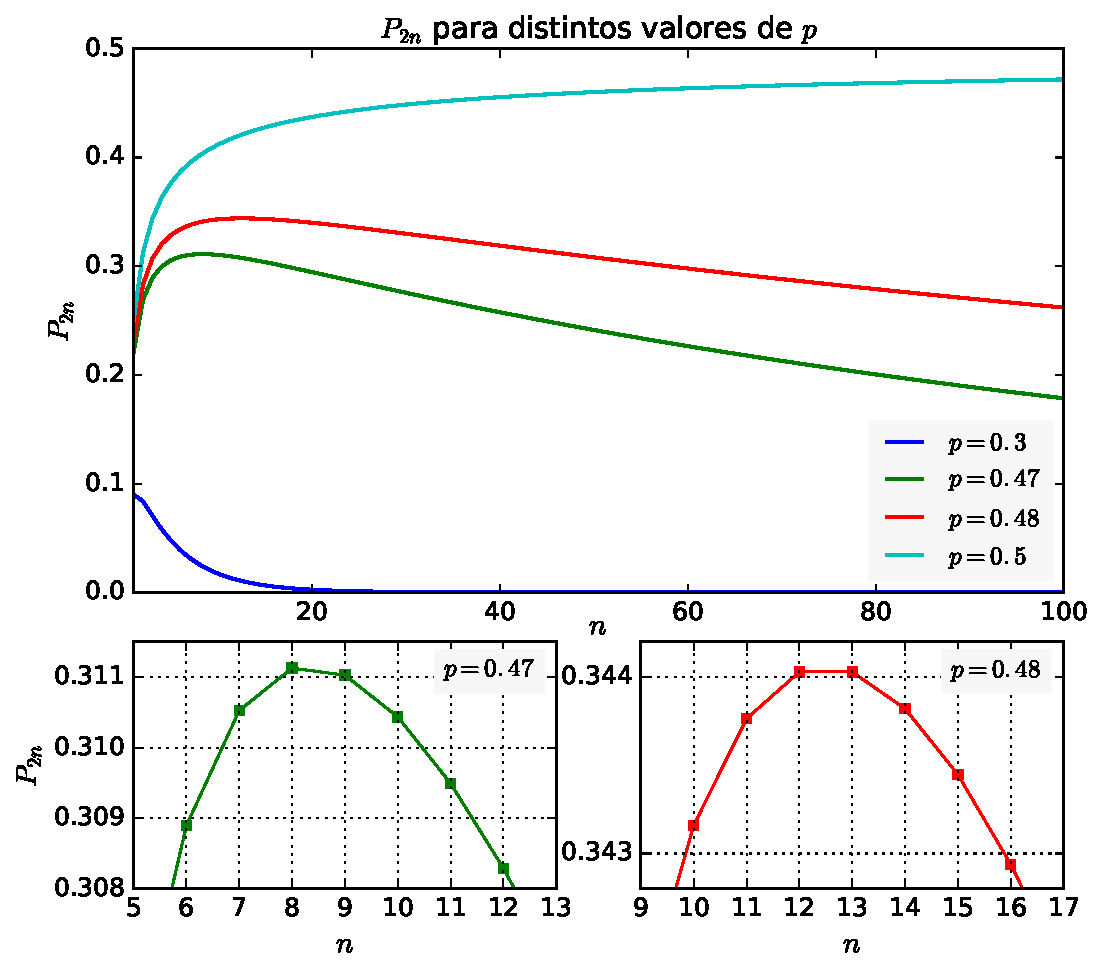
\includegraphics[width=0.9\columnwidth]{figuras/unfair_win_probabilities_v2.pdf}
\caption{\label{fig:unfair_win_probabilities} Probabilidad \(P_{2n}\) de ganar un juego de \(2n\) partidas para valores de \(p=0.3,\, 0.47,\, 0.48\) y \(0.5\). Como se observa en la gráfica de arriba, en el caso de que el juego es equitativo, es decir, cuando \(p=0.5\), la mejor estrategia es jugar la mayor cantidad de partidas posibles, ya que la probabilidad \(P_{2n}\) de ganar crece al valor asintótico de \(0.5\). En el caso en que el juego es desfavorable, esto es, cuando \(p<0.5\), hay dos posibilidades: (1) si \(p\) no es cercano a 0.5, \(P_{2n}\) es decreciente, y la mejor estrategia es jugar la menor cantidad posible de partidas, que es \(2n=2\). Este es el caso en la gráfica con \(p=0.3\). (2) si \(p\) es cercano a 0.5, \(P_{2n}\) tiene un máximo, lo que implica que hay un número óptimo de partidas. Si se continuara jugando indefinidamente, se perdería con certeza, ya que \(P_{2n}\) tiende a \(0\) con \(n\), como se ve en las gráficas con \(p=0.47\) y \(p=0.48\). En las gráficas de abajo, se muestra \(P_{2n}\) para \(p=0.47\) y \(p=0.48\) en torno al máximo. En el caso en que \(p=0.47\), el máximo está en \(n=8\), por lo que el número óptimo de partidas es \(2n=16\). En el caso en que \(p=0.48\), el valor máximo de \(P_{2n}\) se da en dos valores de \(n\), \(n=12\) y \(n=13\), por lo que conviene jugar \(2n=24\) o \(2n=26\) partidas indistintamente. Esto ocurre porque \(1/(1-2p)=25\) es un entero impar, y los dos enteros pares adyacentes producen la misma probabilidad óptima de ganar.}
\end{center}
\end{figure}
De forma similar, si \(2n\) es óptimo, se tiene que cumplir que \(P_{2n}\geq P_{2n-2}\). La relación entre \(P_{2n}\) y \(P_{2n-2}\) se obtiene de la ecuación \ref{eq:unfair_p2n_relation} reemplazando \(n\) por \(n-1\), lo que resulta en
\[
 P_{2n}=P_{2n-2}+\binom{2n-2}{n-1}p^{n+1}q^{n-1}-\binom{2n-2}{n}\,p^{n}q^{n},
\]
y por lo tanto, se debe cumplir que
\[
 \binom{2n-2}{n-1}p^{n+1}q^{n-1}\geq \binom{2n-2}{n}\,p^{n}q^{n}.
\]
Despejando \(n\) igual que antes, se llega a que
\begin{equation}\label{eq:unfair_n_opt_sup}
 n\leq \frac{q}{1-2p},
\end{equation}
y combinando las ecuaciones \ref{eq:unfair_n_opt_inf} y \ref{eq:unfair_n_opt_sup} se obtiene que
\[
 \frac{p}{1-2p}\leq n\leq \frac{q}{1-2p},
\]
o equivalentemente,
\[
 \frac{1}{1-2p}-1\leq 2n\leq \frac{1}{1-2p}+1.
\]
De esta forma, \(2n\) queda determinado unívocamente como el entero par mas cercano a \(1/(1-2p)\). Por ejemplo, si \(p=0.47\), \(1/(1-2p)=16.666\dots\), por lo que el número óptimo de partidas es \(2n=16\). Sin embargo, si \(1/(1-2p)\) es un entero impar, los dos enteros pares adyacentes \(1/(1-2p)-1\) y \(1/(1-2p)+1\) producen la misma probabilidad óptima. Por ejemplo, si \(p=0.48\), \(1/(1-2p)=25\) y el número óptimo de partidas es \(2n=24\) o \(2n=26\), ambos con la misma probabilidad máxima de ganar. En la figura \ref{fig:unfair_win_probabilities} se muestra la probabilidad \(P_{2n}\) de ganar el juego para algunos valores de \(p\). 

\chapter{El concepto de variable aleatoria}

Este capítulo contiene algunos conceptos desarrollados en el capítulo 4 de \cite{papoulis2002probability}.

\section{Variable aleatoria}

Una variable aleatoria es una \emph{función} cuyo dominio es el conjunto \(S\) de todos los resultados posibles de un experimento. Concretamente, un experimento está definido por el espacio muestral \(S\) (o \(\Omega\)), el \(\sigma\)-álgebra de subconjuntos de \(S\), denominados eventos, y una medida de probabilidad asignada a esos eventos. A cada resultado \(\zeta\) del experimento, se asigna un número \(\x(\zeta)\). De esta forma, se creó una función \(\x\) cuyo dominio es el conjunto \(S\) y el rango es un conjunto de números.

Respecto a la notación, se empleará el símbolo \(\x(\zeta)\) para referirse al número asignado al resultado \(\zeta\) específico, y el símbolo \(\x\) para indicar la regla de correspondencia entre los elementos de \(S\) y el número asignado a éstos.

\subsection{Eventos generados por variables aleatorias}

En el estudio de variables aleatorias, surgen preguntas del tipo ``¿Cuál es la probabilidad de que la variable aleatoria \(\x\) sea menor que cierto valor \(x\)?'', o ``¿Cuál es la probabilidad de que la variable aleatoria \(\x\) esté entre los números \(x_1\) y \(x_2\)?'' Debido a que las probabilidades se asignan a eventos, para poder responder esas preguntas, hay que expresar las condiciones impuestas a la variable aleatoria \(\x\) como eventos. En este sentido, considérese la expresión
\[
 \{\x\leq x\}.
\]
Este evento es el subconjunto de \(S\) que consiste en los elementos \(\zeta\) que cumplen que \(\x(\zeta)\leq x\). De esta forma, \(\{\x\leq x\}\) no es un conjunto de números, sino un conjunto de resultados elementales del experimento. Análogamente, la expresión
\[
 \{x_1\leq\x\leq x_2\},
\]
es el subconjunto de \(S\) que contiene los elementos \(\zeta\) tales que \(x_1\leq\x(\zeta)\leq x_2\). De la misma forma, si \(R\) es un conjunto de números del eje \(x\),
\[
 \{x\in R\}
\]
representa el subconjunto de \(S\) que contiene los elementos \(\zeta\) que cumplen que \(\x(\zeta)\in R\). Un comentario adicional de este caso: \(\{x\in R\}\) es un evento solo si \(R\) es la unión e intersección contable de intervalos del eje \(x\). Esta restricción tiene mas interés matemático que práctico.

\subsection{Definición de variable aleatoria}

Formalmente, una variable aleatoria \(\x\) es el proceso de asignación de un número \(\x(\zeta)\) a cada elemento \(\zeta\) del espacio muestral. Esta función de asignación es mas bien arbitraria, siempre que satisfaga las siguientes condiciones:
\begin{enumerate}[I.]
 \item El conjunto \(\{\x\leq x\}\) es un evento para todo \(x\).
 \item Las probabilidades de los eventos \(\{x=-\infty\}\) y \(\{x=\infty\}\) es nula:
 \[
  P\{x=-\infty\}=0\qquad P\{x=\infty\}=0.
 \]
 Esta condición indica que si bien se permite que \(\x(\zeta)=-\infty\) o \(\x(\zeta)=\infty\) para algunos elementos \(\zeta\) del espacio muestral, se exige que el conjunto de estos elementos tenga probabilidad nula.
\end{enumerate}






\section{Distribución y densidad de probabilidad}

\subsection{La función distribución de probabilidad}

Los elementos del espacio muestral \(S\) contenidos en el evento \(\{\x\leq x\}\) cambian al cambiar el número \(x\). Por lo tanto, la probabilidad \(P\{\x\leq x\}\) del evento \(\{\x\leq x\}\) es un número que depende de \(x\). Este número se denota como \(F_x(x)\) y se llama \emph{función de distribución (acumulada)} de la variable aleatoria \(\x\). Es decir, la función de distribución de una variable aleatoria \(\x\) se define como
\[
 F_x(x)=P\{\x\leq x\},
\]
para todo \(x\) desde \(-\infty\) a \(\infty\).

\paragraph{Variables aletorias continuas y discretas}

Se dice que una variable aleatoria \(\x\) es \emph{continua} si su distribución de probabilidad \(F_x(x)\) es continua. En este caso, se puede demostrar que se cumple que \(P\{\x=x\}=0\) para todo \(x\).

Si \(F_x(x)\) es constante excepto por un número finito de discontinuidades de salto (constante a trozos), se dice que \(\x\) es una variable aleatoria \emph{discreta}. Si \(x_i\) es uno de los puntos de discontinuidad, se puede demostrar que se cumple que
\[
 P\{\x=x_i\}=F_x(x_i)-F_x(x^-_i)=p_i.
\]

\paragraph{Percentiles}

Se define el percentil \(u\) de la variable aleatoria \(\x\) como el menor valor \(x_u\) tal que
\[
 u=P\{\x\leq x_u\}=F_x(x_u).
\]
De esta forma, \(x_u=F^{-1}(u)\), por lo que su dominio es el intervalo \(0\leq u \leq 1\) y su rango es el eje \(x\). La \emph{mediana} de \(\x\) es el menor valor \(m\) tal que \(F_x(m)=0.5\). Por lo tanto, la mediana \(m\) es el percentil 0.5 de \(\x\).

Supóngase que se dispone de una serie de observaciones de una variable aleatoria \(\x\) y se desea estimar cierto percentil. Esto se denomina \emph{perceptil empírico}. Por ejemplo, supóngase que hay 100 observaciones y se quiere calcular el percentil 0.6. Esto implica encontrar el valor \(x_{0.6}\) de forma que \(P\{\x\leq x_{0.6}\}=0.6\). Desde el punto de vista de la interpretación en frecuencia de la probabilidad, una probabilidad de 0.6 significa que hay 60 casos favorables entre los 100 casos posibles. Por lo tanto, estimar el percentil 0.6 significa encontrar la observación \(x_{0.6}\) tal que haya 60 observaciones de valor menor o igual a \(x_{0.6}\). Entonces, para encontrar este valor, hay que ordenar las 100 observaciones de menor a mayor, y la observación en la posición 60 es el percentil 0.6 buscado \(x_{0.6}\). Asimismo, la mediana de la variable aleatoria \(\x\), que por definición es el percentil 0.5, es el valor de centro de las observaciones ordenadas de menor a mayor.


\paragraph{Distribución y percentil empíricos}

Supóngase que se realiza un experimento \(n\) veces y se obtienen los valores \(x_1,\,\dots,\,x_n\) de la variable aleatoria \(\x\). Estos valores se ubican en el eje \(x\) y se construye una función \(F_n(x)\) escalonada como se muestra en la figura \ref{fig:percentiles_frequency_interpretation}. Los escalones se ubican en los valores \(x_i\) y tienen altura \(1/n\). El primer escalón se ubica en el valor mas pequeño \(x_\textrm{mín}\). De esta forma \(F_n(x)<0\) para \(x<x_\textrm{mín}\). Esta función es la \emph{distribución de probabilidad empírica} de la variable aleatoria \(\x\), ya que para un valor de \(x\) específico, el número de escalones \(n_x\) de \(F_n(x)\) es la cantidad de valores \(x_i\) mas pequeños que \(x\), por lo que \(F_x(x)=n_x/n\). Como \(n_x/n\approx P\{\x\leq x\}\) si \(n\) es grande, se concluye que
\[
 F_n(n)=\frac{n_x}{n}\to P\{\x\leq x\}=F(x)\quad \textrm{con}\quad n\to\infty.
\]

El percentil empírico se construye de la siguiente forma: se forman \(n\) segmentos de longitud \(x_i\) y se ubican verticalmente en orden creciente separados una distancia \(1/n\), y se construye una función escalonada como se muestra en la figura \ref{fig:percentiles_frequency_interpretation}. Esta función es igual a la distribución empírica \(F_n(x)\) si se intercambian los ejes.
\begin{figure}[!htb]
\begin{center}
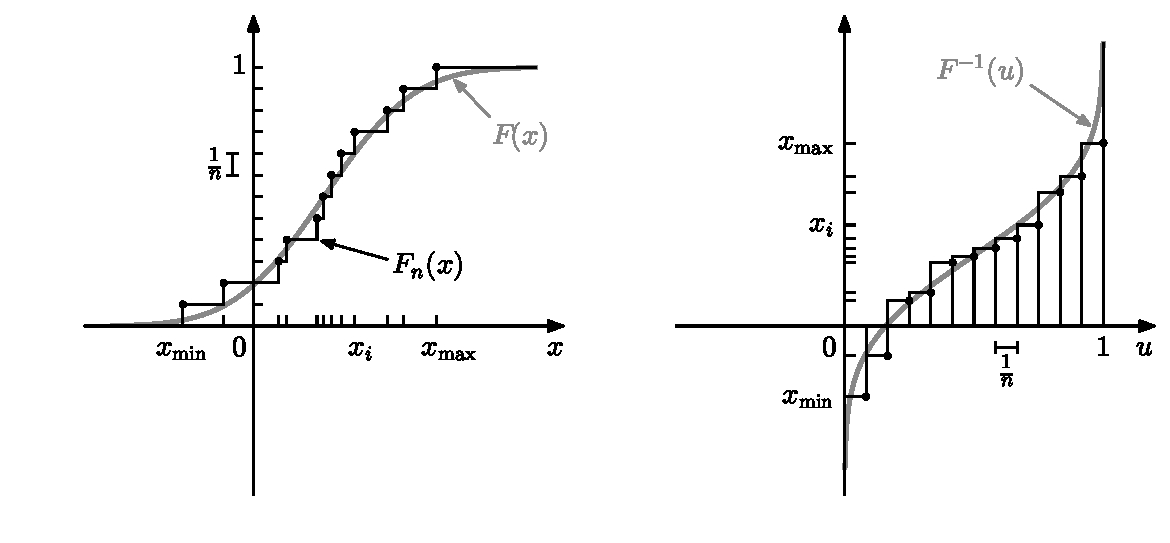
\includegraphics[width=0.9\columnwidth]{figuras/percentiles_frequency_interpretation.pdf}
\caption{\label{fig:percentiles_frequency_interpretation} Distribución y percentil empíricos. En la gráfica de la izquierda se muestra la distribución de probabilidad \(F(x)\) y la distribución empírica \(F_n(x)\) con \(n=12\) para una variable aleatoria normal. A la izquierda se muestra la función inversa \(x_u=F^{-1}(y)\) y el percentil empírico.}
\end{center}
\end{figure}

\subsection{La función densidad de probabilidad}

La derivada de la función distribución de probabilidad \(F_x(x)\) se llama función densidad de probabilidad (p.d.f, \emph{probability density function}) de la variable aleatoria \(\x\) y se denota como \(f_x(x)\). De esta forma
\begin{equation}\label{eq:density_function_definition}
 f_x(x)\triangleq\frac{dF_x(x)}{dx}.
\end{equation}
Si la variable aleatoria \(\x\) es continua, \(f_x(x)\) es una función continua. Si la variable aleatoria \(\x\) es discreta, la densidad de probabilidad tiene la forma
\[
 f_x(x)=\sum_i p_i\delta(x-x_i),
\]
donde \(x_i\) son los puntos de discontinuidad de salto en \(F_x(x)\). En este caso, la densidad es conocida con el nombre de \emph{función de masa de probabilidad} (p.m.f, \emph{probability mass function}).

De la ecuación \ref{eq:density_function_definition}, se deduce que
\[
 F_x(x)=\int_{-\infty}^{x}f_x(u)\,du.
\]
Además, puede probarse que
\begin{equation}\label{eq:density_function_area_between_tow_values}
 P\{x_1<\x\leq x_2\}=F_x(x_2)-F_x(x_1)=\int_{x_1}^{x_2}f_x(x)\,dx,
\end{equation}
es decir, el área bajo la densidad de probabilidad \(f_x(x)\) en el intervalo \((x_1,\,x_2)\) es la probabilidad de que la variable aleatoria \(\x\) pertenezca al intervalo \((x_1,\,x_2)\). 

Si la variable aleatoria \(\x\) es continua, el intervalo en la probabilidad en la ecuación \ref{eq:density_function_area_between_tow_values} puede cambiarse por \(\{x_1\leq\x\leq x_2\}\). Tomando \(x_1=x\) y \(x_2=x+\Delta x\) en la ecuación \ref{eq:density_function_area_between_tow_values}, se obtiene que
\begin{equation}\label{eq:density_definition_as_probability}
 P\{x\leq\x\leq x+\Delta x\}\approx f_x(x)\Delta x
\end{equation}
para \(\Delta x\) suficientemente pequeño. De aquí se obtiene que \(f_x(x)\) puede ser directamente definida como
\begin{equation}\label{eq:density_function_definition_2}
 f_x(x)=\lim_{\Delta x\to0}\frac{P\{x\leq\x\leq x+\Delta x\}}{\Delta x}.
\end{equation}

\section{Variables aleatorias específicas}

En esta sección se describen algunas distribuciones de probabilidad usadas comúnmente. Todo lo aquí mencionado está basado en la sección 4.3 de \cite{papoulis2002probability}. Se hace hincapié en el desarrollo de algunos resultados que no se detallan en la referencia.

\subsection{Variables aleatorias continuas}\label{sec:continuous_random_variables}

\paragraph{Distribución Normal}

Se dice que \(\x\) es una variable aleatoria normal o gaussiana de parámetros \(\mu\) y \(\sigma^2\) si su función densidad de probabilidad es
\begin{equation}\label{eq:pdf_gaussian}
 f_x(x)=\frac{1}{\sqrt{2\pi\sigma^2}}e^{-(x-\mu)^2/2\sigma^2}.
\end{equation}
Se denota \(\x\sim N(\mu,\,\sigma^2)\). 

La constante \(\sqrt{2\pi\sigma^2}\) en la densidad de probabilidad es una constante de normalización para que el área bajo \(f_x(x)\) sea uno. Para ver esto, se demostrará que
\[
 Q\triangleq\int_{-\infty}^{\infty}\,e^{-x^2/2\sigma^2}\,dx=\sqrt{2\pi\sigma^2}.
\]
Es claro que el área bajo \(e^{-x^2/2\sigma^2}\) coincide con el área bajo \(e^{-(x-\mu)^2/2\sigma^2}\) de la ecuación \ref{eq:pdf_gaussian}, ya que el cambio de variable \(x-\mu\) es solo en un desplazamiento de la curva en \(x\) una cantidad \(\mu\).
Considérese
\begin{align}\label{eq:random_gaussian_integral_result_1}
 Q^2&=\left(\int_{-\infty}^{\infty}\,e^{-x^2/2\sigma^2}\,dx\right)^2\nonumber\\
   &=\left(\int_{-\infty}^{\infty}\,e^{-x^2/2\sigma^2}\,dx\right)\left(\int_{-\infty}^{\infty}\,e^{-y^2/2\sigma^2}\,dy\right)\nonumber\\
   &=\int_{-\infty}^{\infty}\int_{-\infty}^{\infty}\,e^{-(x^2+y^2)/2\sigma^2}\,dx\,dy
\end{align}
La integral doble es una integral en todo el plano \((x,\,y)\). Se realizará el cambio de variable
\begin{equation}\label{eq:random_polar_coordinates_transform}
 x=r\cos\theta,\qquad y=r\sin\theta,
\end{equation}
que consiste en transformar la integral doble en coordenadas cartesianas a coordenadas polares. Para hacerlo, recordar que para integrar \(f(x,\,y)\) sobre la región \(R\) del plano, bajo la transformación \(x=g(u,\,v)\), \(x=h(u,\,v)\), la región de integración se transforma en \(S\) y la integral es
\begin{equation}\label{eq:random_double_integral_variable_change}
 \iint_{R}f(x,\,y)dA=\iint_{S}f(g(u,\,v),\,h(u,\,v))|J(u,\,v)|du\,dv,
\end{equation}
donde \(|J(u,\,v)|\) es el determinante de la matriz Jacobiana. En el caso de la transformación a coordenadas polares dada por la ecuación \ref{eq:random_polar_coordinates_transform}, la matriz Jacobiana es
\[
 J(r,\,\theta)=
 \begin{pmatrix}
    \partial x/\partial r & \partial x/\partial \theta \\
    \partial y/\partial r & \partial y/\partial \theta
\end{pmatrix}=
 \begin{pmatrix}
    \cos\theta & -r\sin\theta \\
    \sin\theta & r\cos\theta
 \end{pmatrix},
\]
y el determinante es \(|J(r,\,\theta)|=r\), por lo que al aplicar la transformación de la ecuación \ref{eq:random_double_integral_variable_change} a la ecuación \ref{eq:random_gaussian_integral_result_1} notando que \(x^2+y^2=r^2\) se obtiene que
\begin{align*}
 Q^2&=\int_{0}^{2\pi}\int_{0}^{\infty}\,e^{-r^2/2\sigma^2}r\,dr\,d\theta\\
    &=2\pi\int_{0}^{\infty}\,e^{-r^2/2\sigma^2}r\,dr\\
    &\overset{(a)}{=}2\pi\sigma^2\int_{0}^{\infty}\,e^{-u}\,du\\
    &=2\pi\sigma^2,
\end{align*}
donde en \((a)\) se realizó el cambio de variable \(u=r^2/2\sigma^2\), \(rdr=\sigma^2du\). Se concluye que
\begin{equation}\label{eq:random_gaussian_integral_with_sigma}
  \int_{-\infty}^{\infty}\,e^{-x^2/2\sigma^2}\,dx = \sqrt{2\pi\sigma^2}
\end{equation}
En el caso en que \(\sigma^2=1/2\), la ecuación anterior queda
\begin{equation}\label{eq:random_gaussian_integral}
 \int_{-\infty}^{\infty}\,e^{-x^2}\,dx = \sqrt{\pi},
\end{equation}
resultado que se conoce como integral gaussiana\footnote{ver \url{https://en.wikipedia.org/wiki/Gaussian_integral}}.

\paragraph{Distribución Exponencial}

La variable aleatoria \(\x\) es exponencial de parámetro \(\lambda\) si su densidad de probabilidad es
\begin{equation}\label{eq:pdf_exponential}
 f_x(x)=
 \left\{\begin{array}{ll}
  \lambda e^{-\lambda x}, & x\geq 0 \\
  0, & \textrm{en otro caso}
 \end{array}. \right.
\end{equation}
Si la ocurrencia de eventos en intervalos de tiempo que no se solapan son independientes, como los instantes de ocurrencia de llamadas telefónicas o los instantes de arribo de ómnibus a una parada, puede demostrarse que el tiempo de espera de esos eventos es una variable aleatoria exponencial. 

La distribución de probabilidad de una variable aleatoria exponencial es
\[
 F_x(x)=1-e^{-\lambda x}.
\]
Para verlo, se parte de la definición de densidad de probabilidad y se opera de la siguiente forma,
\begin{align*}
 F_x(x)&=\int_{-\infty}^{x}f_x(u)du\\
       &=\int_{0}^{x}\lambda e^{-\lambda u}du\\
       &=-e^{-\lambda u}\Big|_{0}^{x}\\
       &=-\left(e^{-\lambda x}-1\right)\\
       &=1-e^{-\lambda x}.
\end{align*}
De forma similar, puede probarse que la media de una variable aleatoria exponencial \(\x\) es \(E\{\x\}=1/\lambda\). El concepto de media y varianza se desarrolla mas adelante en \cite{papoulis2002probability}, pero se incluye aquí por conveniencia. Usando la definición de la media de una variable aleatoria y operando, se tiene que
\begin{align*}
 E\{\x\}&=\int_{-\infty}^{\infty}tf_x(t)dt\\
        &=\int_{0}^{\infty}t\lambda e^{-\lambda t}dt\\
        &\overset{(a)}{=}-te^{-\lambda t}\Big|_{0}^{\infty}+\int_{0}^{\infty}e^{-\lambda t}dt\\
        &=-\frac{1}{\lambda}e^{-\lambda t}\Big|_{0}^{\infty}\\
        &=-\frac{1}{\lambda}(0-1)\\
        &=\frac{1}{\lambda},
\end{align*}
donde en \((a)\) se aplicó integración por partes, \(\int udv=uv-\int vdu\), con \(u=t\) y \(dv=\lambda e^{-\lambda t}\), y entonces \(du=1\) y \(v=-e^{-\lambda t}\). Esto implica que si la variable aleatoria exponencial \(\x\) es por ejemplo cierto tiempo de espera de ocurrencia de un evento, su media es \(1/\lambda\) unidades de tiempo y \(\lambda\) es la tasa de ocurrencia del evento. En ocasiones, en lugar de la parametrización con \(\lambda\) se emplea el parámetro \(\beta=1/\lambda\). En este caso, 
\[\def\arraystretch{2.0}
 f_x(x)=
 \left\{\begin{array}{ll}
  \dfrac{1}{\beta} e^{-x/\beta}, & x\geq 0\\
  0, & \textrm{en otro caso}
 \end{array}, \right.
\]
y \(E\{\x\}=\beta\).

\paragraph{Distribución Gamma}

Se dice que \(\x\) es una variable aleatoria gamma de parámetros \(\alpha\) y \(\beta\), \(\alpha\geq 0,\,\beta\geq 0\), si su densidad de probabilidad es
\begin{equation}\label{eq:pdf_gamma}
\def\arraystretch{2.0}
 f_x(x)=
 \left\{\begin{array}{ll}
  \dfrac{x^{\alpha-1}}{\Gamma(\alpha)\beta^\alpha} e^{-x/\beta}, & x\geq 0\\
  0, & \textrm{en otro caso}
 \end{array}, \right.
\end{equation}
donde \(\Gamma(\alpha)\) es la función gamma, definida como
\begin{equation}\label{eq:gamma_function}
 \Gamma(\alpha)=\int_{0}^{\infty}x^{\alpha-1}e^{-x}\,dx.
\end{equation}

A continuación se mencionarán algunas propiedades de la función gamma. La función gamma cumple la ecuación funcional
\begin{equation}\label{eq:gamma_functional_equation}
 \Gamma(\alpha)=(\alpha-1)\Gamma(\alpha-1).
\end{equation}
Para verlo, se parte de la definición de la función gamma y se opera de la siguiente forma, 
\begin{align*}
 \Gamma(\alpha)&=\int_{0}^{\infty}x^{\alpha-1}e^{-x}\,dx\\
   &\overset{(a)}{=}-x^{\alpha-1}e^{-x}\Big|_{0}^{\infty}+(\alpha-1)\int_{0}^{\infty}x^{\alpha-2}e^{-x}\,dx\\
   &=(\alpha-1)\Gamma(\alpha-1),
\end{align*}
donde en \((a)\) se aplicó integración por partes con \(u=x^{\alpha-1}\) y \(dv=e^{-x}\), y entonces \(du=(\alpha-1)x^{\alpha-2}\) y \(v=-e^{-x}\).
Si \(\alpha=n\) es un número entero, se cumple que
\begin{equation}\label{eq:gamma_function_equals_factorial}
 \Gamma(n)=(n-1)\Gamma(n-1)=(n-1)!,
\end{equation}
ya que
\[
 \Gamma(1)=\int_{0}^{\infty}e^{-x}\,dx=-e^{-x}\Big|_{0}^{\infty}=-(0-1)=1.
\]
y por lo tanto
\[
 \Gamma(n)=(n-1)\Gamma(n-1)=(n-1)(n-2)\cdots 2\cdot 1\cdot\Gamma(1)=(n-1)!.
\]
Se cumple además que
\[
 \Gamma(1/2)=\sqrt{\pi}.
\]
Efectivamente, evaluando la función gamma en \(\alpha=1/2\) y operando, se tiene que 
\begin{align*}
 \Gamma(1/2)&=\int_{0}^{\infty}x^{1/2-1}e^{-x}\,dx\\
   &=\int_{0}^{\infty}x^{-1/2}e^{-x}\,dx\\
   &\overset{(a)}{=}-x^{1/2}e^{-x}\Big|_{0}^{\infty}+2\int_{0}^{\infty}e^{-u^2}\,du\\
   &=\int_{-\infty}^{\infty}e^{-x^2}\,dx\\
   &\overset{(b)}{=}\sqrt{\pi},
\end{align*}
donde en \((a)\) se aplicó integración por partes con \(u=x^{1/2}\) y \(dv=e^{-x}\,dx\), y entonces \(du=(1/2)x^{-1/2}\,dx\) y \(v=-e^{-x}\), y en \((b)\) se notó que la integral es gaussiana y se aplicó el resultado de la ecuación \ref{eq:random_gaussian_integral}.
Empleando la ecuación \ref{eq:gamma_functional_equation}, se deduce que
\[\arraycolsep=2pt\def\arraystretch{2.5}
\begin{array}{ccccc}
  \Gamma\left(\dfrac{3}{2}\right)&=&\dfrac{1}{2}\,\Gamma\left(\dfrac{1}{2}\right)&=&\dfrac{\sqrt{\pi}}{2}\\
  \Gamma\left(\dfrac{5}{2}\right)&=&\dfrac{3}{2}\,\Gamma\left(\dfrac{3}{2}\right)&=&\dfrac{3\sqrt{\pi}}{4},
\end{array}
\]
y así sucesivamente, resultando en el caso general, en
\begin{align*}
 \Gamma\left(\frac{2n+1}{2}\right)&=\dfrac{(2n-1)(2n-3)\cdots5\cdot3\cdot1}{2^n}\sqrt{\pi}\\
 &\overset{(a)}{=}\dfrac{(2n-1)!!}{2^n}\sqrt{\pi}\\
 &\overset{(b)}{=}\dfrac{(2n)!}{4^nn!}\sqrt{\pi}
\end{align*}
donde en \((a)\) se expresó la ecuación empleando la operación de doble factorial\footnote{Ver \url{https://en.wikipedia.org/wiki/Double_factorial}.} y en \((b)\) se tuvieron las siguientes consideraciones. Por un lado, para un número par \(2n\), se cumple que
\[
 (2n)!!=(2n)(2n-2)(2n-4)\cdots4\cdot2\overset{(a)}{=}2^nn(n-1)(n-2)\cdots2\cdot1=2^nn!,
\]
donde en \((a)\) se sacó 2 de factor común en cada uno de los \(n\) factores del producto.
Por otro lado, es fácil ver que
\[
 n!=n!!(n-1)!!\qquad\Rightarrow\qquad n!!=\frac{n!}{(n-1)!!}=\frac{n!(n+1)}{(n-1)!!(n+1)}=\frac{(n+1)!}{(n+1)!!}.
\]
Empleando estos dos resultados, se observa que para un número impar \(2n-1\), se cumple que
\[
 (2n-1)!!=\frac{(2n)!}{(2n)!!}=\frac{(2n)!}{2^nn!},
\]
que es lo que se quería mostrar.



Una variable aleatoria \(\x\) gamma de parámetros \(\alpha\) y \(\beta\) se denota como \(\x\sim G(\alpha,\, \beta)\). La función de densidad gamma tiene un conjunto variado de formas en función del valor de los parámetros \(\alpha\) y \(\beta\). Una variable aleatoria exponencial es un caso particular de una variable aleatoria gamma con \(\alpha=1\). Con \(\alpha=n/2\) y \(\beta=2\) se obtiene una variable aleatoria \(\chi^2\) (chi-cuadrado) con \(n\) grados de libertad.

Con \(\alpha=n\) entero en la ecuación \ref{eq:pdf_gamma} y definiendo \(\beta=1/\lambda\), la función densidad de probabilidad gamma es
\begin{equation}\label{eq:pdf_gamma_integer}
\def\arraystretch{2.0}
 f_x(x)=
 \left\{\begin{array}{ll}
  \dfrac{\lambda^nx^{n-1}}{(n-1)!} e^{-\lambda x}, & x\geq 0\\
  0, & \textrm{en otro caso.}
 \end{array} \right.
\end{equation}
Se demostrará a continuación que la distribución de probabilidad es
\[
 F_x(t)=1-\sum_{k=0}^{n-1}\frac{(\lambda t)^k}{k!}e^{-\lambda t}.
\]
Para hacerlo, se parte de la definición de distribución de probabilidad y se aplica integración por partes,
\begin{align*}
 F_x(t)&=\int_{0}^{t}f_x(x)\,dx\\
   &=\frac{\lambda^n}{(n-1)!}\int_{0}^{t}x^{n-1}e^{-\lambda x}\,dx\\
   &=\frac{\lambda^{n-1}}{(n-2)!}\int_{0}^{t}\frac{x^{n-1}}{n-1}\lambda e^{-\lambda x}\,dx\\
   &\overset{(a)}{=}\frac{\lambda^{n-1}}{(n-2)!}\left(-\frac{x^{n-1}e^{-\lambda x}}{n-1}\bigg|_{0}^{t}+\int_{0}^{t}x^{n-2}e^{-\lambda x}\,dx\right)\\
   &=\frac{\lambda^{n-1}}{(n-2)!}\left(-\frac{t^{n-1}e^{-\lambda t}}{n-1}+\int_{0}^{t}x^{n-2}e^{-\lambda x}\,dx\right)\\
   &=-\frac{(\lambda t)^{n-1}e^{-\lambda t}}{(n-1)!}+\frac{\lambda^{n-1}}{(n-2)!}\int_{0}^{t}x^{n-2}e^{-\lambda x}\,dx,
\end{align*}
donde en \((a)\) se aplicó integración por partes con \(u=x^{n-1}/(n-1)\) y \(dv=\lambda e^{-\lambda x}\), y entonces \(du=x^{n-2}\) y \(v=-e^{-\lambda x}\). Notar que el segundo sumando en la última ecuación es la distribución de probabilidad gamma con parámetro \(\alpha=n-1\).
Aplicando integración por partes \(n-2\) veces mas, es decir, \(n-1\) veces en total, se obtiene que
\begin{align*}
 F_x(t)&=-\frac{(\lambda t)^{n-1}e^{-\lambda t}}{(n-1)!}-\frac{(\lambda t)^{n-2}e^{-\lambda t}}{(n-2)!}-\dots-\frac{(\lambda t)e^{-\lambda t}}{1!}+\frac{\lambda}{0!}\int_{0}^{t}e^{-\lambda x}\,dx\\
   &=-\frac{(\lambda t)^{n-1}e^{-\lambda t}}{(n-1)!}-\frac{(\lambda t)^{n-2}e^{-\lambda t}}{(n-2)!}-\dots-\frac{(\lambda t)e^{-\lambda t}}{1!}-e^{-\lambda t}+1\\
   &=1-\sum_{k=0}^{n-1}\frac{(\lambda t)^k}{k!}e^{-\lambda t}.
\end{align*}

\paragraph{Distribución chi-cuadrado}

Se dice que una variable aleatoria \(\x\) es \(\chi^2(n)\) (chi-cuadrado) con \(n\) grados de libertad si su densidad de probabilidad es
\begin{equation}\label{eq:pdf_chi_square}
\def\arraystretch{2.0}
 f_x(x)=
 \left\{\begin{array}{ll}
  \dfrac{x^{n/2-1}}{2^{n/2}\Gamma(n/2)} e^{-x/2}, & x\geq 0\\
  0, & \textrm{en otro caso}
 \end{array}, \right.
\end{equation}
donde \(\Gamma(\alpha)\) es la función gamma definida en la ecuación \ref{eq:gamma_function}.


\paragraph{Otras distribuciones}

En la referencia bibliográfica utilizada (\cite{papoulis2002probability}), se describe con cierto detalle otros tipos de variables aleatorias continuas. Se mencionarán a continuación algunas de ellas de forma breve. 

La \emph{variable aleatoria de Erlang} es un caso particular de la variable aleatoria gamma con \(G(n,\, 1/n\mu)\). Cuando el parámetro \(n\) entero de la distribución de Erlang es \(1\), se obtiene una distribución exponencial, y cuando \(n\to\infty\) se obtiene una distribución constante \(F_x(t)=1\) para \(t>1/\mu\) y cero en otro caso. Por lo tanto, la distribución de Erlang abarca  de aleatoriedad a certeza cuando \(n\) varía 1 a \(\infty\).

La \emph{distribución beta} toma una cantidad variada de formas en un soporte acotado, por ejemplo, en \((0,\, 1)\), y por lo tanto, es una distribución mas flexible que la distribución uniforme.

Otras distribuciones mencionadas en \cite{papoulis2002probability} son: Rayleigh, Nakagami, uniforme, Cauchy, Laplace y Maxwell.

\subsection{Variables aleatorias discretas}\label{sec:discrete_random_variables}

\paragraph{Distribución de Bernoulli} 

La variable aleatoria \(\x\) es Bernoulli si toma valores 0 o 1 con probabilidad
\[
 P\{\x=1\}=p,\qquad\qquad P\{\x=0\}=q=1-p.
\]

\paragraph{Distribución Binomial}

En \(n\) ensayos Bernoulli independientes donde \(p\) es la probabilidad de éxito de cada ensayo, si \(\y\) es la cantidad de éxitos en los \(n\) experimentos, \(\y\) es una variable aleatoria Binomial. Por lo tanto, se dice que \(\y\) es una variable aleatoria Binomial de parámetros \(n\) y \(p\) si \(\y\) toma valores \(0,\,1,\,2,\dots,\,n\) con probabilidad
\[
 P\{\y=k\}=\binom{n}{k}p^{k}q^{n-k},\qquad p+q=1,\qquad k=0,\,1,\,2,\dots,\,n.
\]

\paragraph{Distribución de Poisson}

La distribución de Poisson representa el número de ocurrencias de un evento poco frecuente en un número grande de ensayos. La variable aleatoria \(\x\) se dice Poisson con parámetro \(\lambda\) si toma valores \(0,\,1,\,2,\dots,\,\infty\) con probabilidad
\[
 P\{\x=k\}=e^{-\lambda}\frac{\lambda^k}{k!},\qquad k=0,\,1,\,2,\dots,\,\infty.
\]

\section{Distribuciones condicionales}\label{sec:conditional_distributions}

Todo lo incluido en esta sección está basado en la sección 4.4 de \cite{papoulis2002probability}.

En la sección \ref{sec:conditional_probability_events} se definió la probabilidad condicional de eventos. La \emph{distribución condicional} \(F(x|M)\) de la variable aleatoria \(\x\) dado el evento \(M\) se define como la probabilidad condicional del evento \(\{\x\leq x\}\),
\begin{equation}\label{eq:conditional_distribution_definition}
 F(x|M)=P\{\x\leq x|M\}=\frac{P\{\x\leq x,\,M\}}{P(M)},
\end{equation}
donde \(\{\x\leq x,\,M\}\) es la intersección de los eventos \(\{\x\leq x\}\) y \(M\), es decir, el evento que consiste en todos los resultados \(\zeta\) tal que \(\x(\zeta)\leq x\) y \(\zeta\in M\). \(F(x|M)\) tiene todas las propiedades de una distribución de probabilidad. En particular, se cumple que
\[
 F(\infty|M)=1\qquad F(-\infty|M)=0
\]
\[
 P\{x_1<\x\leq x_2|M\}=F(x_2|M)-F(x_1|M)=\frac{P\{x_1<\x\leq x_2,\,M\}}{P(M)}.
\]

La \emph{densidad condicional} \(f(x|M)\) es la derivada de \(F(x|M)\),
\[
 f(x|M)=\frac{dF(x|M)}{dx}=\lim_{\Delta x\to 0}\frac{P\{x<\x\leq x+\Delta x|M\}}{\Delta x}.
\]
Por ser una densidad de probabilidad es una función nonegativa de área 1.

En general, para determinar \(F(x|M)\) es necesario conocer el experimento subyacente. Sin embargo, si \(M\) puede expresarse en función de la variable aleatoria \(\x\), alcanza con conocer \(F(x)\) para determinar \(F(x|M)\). A continuación se presentan dos casos como ejemplo.
\begin{enumerate}[I.]
 \item Se quiere encontrar la distribución condicional de la variable aleatoria \(\x\) dado \(\x\leq a\), asumiendo que \(F(a)\neq 0\). Esto es un caso especial de la ecuación \ref{eq:conditional_distribution_definition} con \(M=\{\x\leq a\}\). Por lo tanto, como indica la ecuación, el problema consiste en encontrar la función
 \[
  F(x|\x\leq a)=P\{\x\leq x|\x\leq a\}=\frac{P\{\x\leq x,\,\x\leq a\}}{P\{\x\leq a\}}.
 \]
 \begin{itemize}
  \item Si \(x\geq a\), se cumple que \(\{\x\leq x,\,\x\leq a\}=\{\x\leq a\}\), ya que \(\{\x\leq a\}\subset\{\x\leq x\}\). Por lo tanto,
 \[
  F(x|\x\leq a)=\frac{P\{\x\leq a\}}{P\{\x\leq a\}}=1,\qquad x\geq a.
 \]
 \item Si \(x < a\), se cumple que \(\{\x\leq x,\,\x\leq a\}=\{\x\leq x\}\) y por lo tanto,
 \[
  F(x|\x\leq a)=\frac{P\{\x\leq x\}}{P\{\x\leq a\}}=\frac{F(x)}{F(a)},\qquad x<a.
 \]
 \end{itemize}
 Es decir
 \begin{equation}\label{eq:rv_conditional_distribution_x_leq_a}
 F(x|\x\leq a)=
 \left\{\begin{array}{ll}
 \dfrac{F(x)}{F(a)}, & x<a.\\
  \\
  1, & x\geq a \\
 \end{array} \right.
 \end{equation}
 Para obtener la densidad condicional, hay que derivar \(F(x|\x\leq a)\) respecto a \(x\). Como \(F'(x)=f(x)\), se obtiene que
 \begin{equation}\label{eq:rv_conditional_density_x_leq_a}
   f(x|\x\leq a)=
 \left\{\begin{array}{ll}
 \dfrac{f(x)}{F(a)}=\dfrac{f(x)}{\int_{-\infty}^{a}f(x)dx}, & x<a.\\
  \\
  0, & x\geq a \\
 \end{array} \right.
 \end{equation}
 \item Se supone ahora que \(M=\{b<\x\leq a\}\), por lo que la ecuación \ref{eq:conditional_distribution_definition} queda
 \[
  F(x|b<\x\leq a)=\frac{P\{\x\leq x,\,b<\x\leq a\}}{P\{b<\x\leq a\}}.
 \]
 \begin{itemize}
  \item Si \(x\geq a\), se cumple que \(\{\x\leq x,\,b<\x\leq a\}=\{b<\x\leq a\}\). Por lo tanto,
 \[
  F(x|b<\x\leq a)=\frac{P\{b<\x\leq a\}}{P\{b<\x\leq a\}}=1,\qquad x\geq a.
 \]
 \item Si \(b\leq x<a\), se cumple que \(\{\x\leq x,\,b<\x\leq a\}=\{b<\x\leq x\}\) y Por lo tanto,
 \[
  F(x|b<\x\leq a)=\frac{P\{b<\x\leq x\}}{P\{b<\x\leq a\}}=\frac{F(x)-F(b)}{F(a)-F(b)},\qquad b\leq x<a.
 \]
 \item Si \(x<b\), se cumple que \(\{\x\leq x,\,b<\x\leq a\}=\{\emptyset\}\). Por lo tanto,
 \[
  F(x|b<\x\leq a)=0,\qquad x<b.
 \]
 \end{itemize}
 Por lo tanto
 \begin{equation}\label{eq:rv_conditional_distribution_b_leq_x_leq_a}
  F(x|b<\x\leq a)=
 \left\{\begin{array}{ll}
  0, & x<b \\
  \\
 \dfrac{F(x)-F(a)}{F(a)-F(b)}, & b\leq x<a.\\
  \\
  1, & x\geq a \\
 \end{array} \right.
 \end{equation}
 Derivando \(F(x|\x\leq a)\) respecto a \(\x\), se obtiene la densidad condicional, que es
 \begin{equation}\label{eq:rv_conditional_density_b_leq_x_leq_a}
  f(x|b<\x\leq a)=
 \left\{\begin{array}{ll}
 \dfrac{f(x)}{F(a)-F(b)}=\dfrac{f(x)}{\int_{b}^{a}f(x)dx}, & b\leq x<a.\\
  \\
  0, & \textrm{en otro caso} \\
 \end{array} \right.
 \end{equation}
\end{enumerate}
En la figura \ref{fig:conditional_distribition_and_density} se ilustran los resultados cuando la variable aleatoria \(\x\) es normal.
\begin{figure}[!htb]
\begin{center}
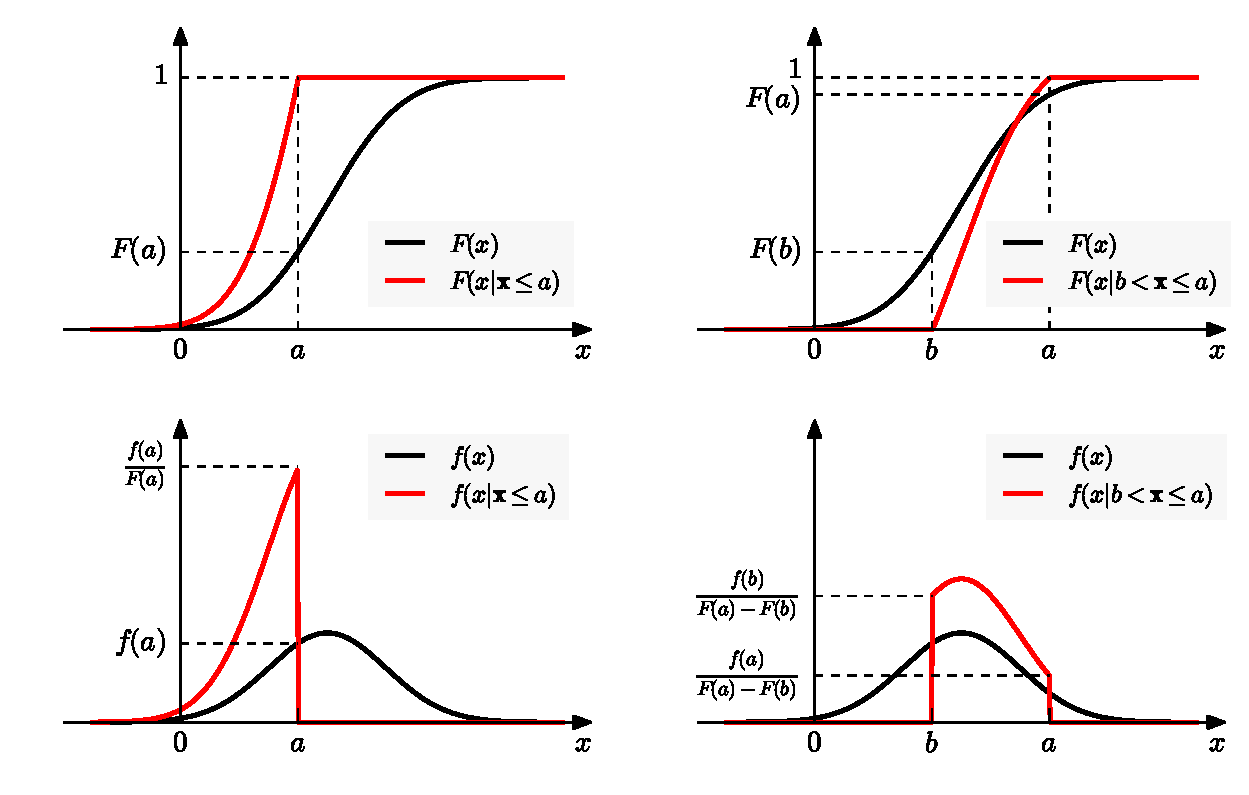
\includegraphics[width=1\columnwidth]{figuras/conditional_distribition_and_density.pdf}
\caption{\label{fig:conditional_distribition_and_density} Distribución \(F(x|M)\) y densidad \(f(x|M)\) condicional cuando \(M\) puede expresarse en términos de \(\x\). En este ejemplo, \(\x\) es una variable aleatoria normal, \(\x\sim N(\mu,\,\sigma^2)\). En las gráficas de la izquierda se muestra la distribución y la densidad en el caso en que \(M=\{\x\leq a\}\), dadas por las ecuaciones \ref{eq:rv_conditional_distribution_x_leq_a} y \ref{eq:rv_conditional_density_x_leq_a} respectivamente. Se usó \(a=\mu-\sigma/2\) en el ejemplo. En las gráficas de la derecha se muestra la distribución y la densidad en el caso en que \(M=\{b< \x\leq a\}\) dadas por las ecuaciones \ref{eq:rv_conditional_distribution_b_leq_x_leq_a} y \ref{eq:rv_conditional_density_b_leq_x_leq_a} respectivamente. Se usó \(b=\mu-\sigma/2\) y \(a=\mu+3\sigma/2\) en el ejemplo.}
\end{center}
\end{figure}

\subsection{Probabilidad total y el teorema de Bayes}

Para extender estos resultados a variables aleatorias, se establece \(B=\{\x\leq x\}\) en la ecuación \ref{eq:total_probability_theorem}
\[
 P(\{\x\leq x\})=P(\x\leq x|A_1)P(A_1)+\cdots+P(\x\leq x|A_n)P(A_n)
\]
y usando las definiciones de distribución y densidad condicional, se obtiene que
\[
\begin{array}{lllllll}
 F(x)&=&F(x|A_1)P(A_1)&+&\cdots&+&F(x|A_n)P(A_n)\\
 f(x)&=&f(x|A_1)P(A_1)&+&\cdots&+&f(x|A_n)P(A_n),
 \end{array}
\]
donde los eventos \(A_1,\,\dots,\,A_n\) forman una partición del espacio muestral \(S\). Procediendo de igual forma con la ecuación \ref{eq:bayes_theorem_for_events_2} se obtiene que
\[
 P\{A|\x\leq x\}=\frac{P\{\x\leq x|A\}}{P\{\x\leq x\}}P(A)=\frac{F(x|A)}{F(x)}P(A).
\]
Estableciendo \(B\) como \(\{x_1<\x\leq x_2\}\) en la ecuación \ref{eq:bayes_theorem_for_events_2} se llega a que
\begin{align*}
 P\{A|x_1<\x\leq x_2\}&=\frac{P\{x_1<\x\leq x_2|A\}}{P\{x_1<\x\leq x_2\}}P(A)\\
    &=\frac{F(x_2|A)-F(x_1|A)}{F(x_2)-F(x_1)}P(A).
\end{align*}
La probabilidad condicional \(P\{A|\x = x\}\) no se puede definir a partir de la ecuación \ref{eq:bayes_theorem_for_events_2} debido a que en general \(P\{\x = x\}=0\), obteniendo un resultado indeterminado, pero si puede hacerse como el siguiente límite
\begin{align*}
 P\{A|\x = x\}&=\lim_{\Delta x\to 0} P\{A|x<\x\leq x+\Delta x\}\\
   &\overset{(a)}{=}\lim_{\Delta x\to 0}\frac{P\{x<\x\leq x+\Delta x|A\}}{P\{x<\x\leq x+\Delta x\}}P(A)\\
   &\overset{(b)}{=}\frac{\lim\limits_{\Delta x\to 0} \dfrac{P\{x<\x\leq x+\Delta x|A\}}{\Delta x}}{\lim\limits_{\Delta x\to 0} \dfrac{P\{x<\x\leq x+\Delta x\}}{\Delta x}}P(A),
\end{align*}
donde en \((a)\) se usó el resultado anterior y en \((b)\) se dividió el numerador y el denominador entre \(\Delta x\) y se aplicó una propiedad de límites. Finalmente, a partir de la definición de densidad y densidad condicional se obtiene que
\begin{equation}\label{eq:rv_p_A_given_x_=_x}
 P\{A|\x = x\}=\frac{f(x|A)}{f(x)}P(A).
\end{equation}

\paragraph{Teorema de la probabilidad total} Como se mencionó previamente, 
\[
 F(\infty|A)=\int_{-\infty}^{\infty}f(x|A)\,dx=1.
\]
Por lo tanto, multiplicando la ecuación \ref{eq:rv_p_A_given_x_=_x} por \(f(x)\) e integrando, se obtiene que
\begin{equation}\label{eq:total_probability_theorem_continuous}
 \int_{-\infty}^{\infty}P\{A|\x = x\}f(x)\,dx=P(A),
\end{equation}
que es la versión continua del teorema de la probabilidad total dada por la ecuación \ref{eq:total_probability_theorem}.

\paragraph{Teorema de Bayes} Despejando \(f(x|A)\) en la ecuación \ref{eq:rv_p_A_given_x_=_x} , se obtiene que
\begin{equation}\label{eq:bayes_theorem_for_events_continuous}
 f(x|A)=\frac{P\{A|\x = x\}}{P(A)}f(x)=\frac{P\{A|\x = x\}f(x)}{\int_{-\infty}^{\infty}P\{A|\x = x\}f(x)\,dx}
\end{equation}
donde en la segunda igualdad se sustituyó \(P(A)\) por el resultado de la ecuación \ref{eq:total_probability_theorem_continuous}. Esta es la versión continua del teorema de Bayes dado por la ecuación \ref{eq:bayes_theorem_for_events}.

\subsection{Ejemplo 4-19}

Sea \(p=P(H)\) la probabilidad de obtener cara al tirar una moneda. Para determinada moneda, la probabilidad a priori \(p\) es desconocida y puede ser cualquier valor en el intervalo \((0,\,1)\). Ante la ausencia de mas información, se debería asumir que la densidad de probabilidad \(f_p(p)\) a priori es uniforme en ese intervalo. De esta forma, no se le da preferencia a algún valor de \(p\) en particular. Supóngase que se realiza el experimento de lanzar la moneda \(n\) veces y se obtiene cara \(k\) veces. Con esta nueva información, ¿cómo se actualiza \(f_p(p)\)?

Sea el evento \(A\)=``\(k\) caras en \(n\) tiradas''. Como en esas \(n\) tiradas se obtiene una secuencia específica de \(k\) caras, se cumple que
\[
 P(A|\p=p)=p^kq^{n-k}=p^k(1-p)^{n-k}.
\]
Usando la ecuación \ref{eq:total_probability_theorem_continuous}, se obtiene que
\begin{align*}
 P(A) &= \int_{-\infty}^{\infty}P\{A|\p = p\}f_p(p)\,dp\\
      &\overset{(a)}{=} \int_{0}^{1}p^k(1-p)^{n-k}\,dp
\end{align*}
en donde en \((a)\) se usó el resultado anterior y que \(f_p(p)=1\) si \(p\in(0,\,1)\) y \(f_p(p)=0\) en otro caso. La última integral puede resolverse aplicando integración por partes \(k\) veces. Al aplicar partes una vez con \(u=p^k\) y \(dv=(1-p)^{n-k}\), por lo que \(du=kp^{k-1}\) y \(v=-(1-p)^{n-k+1}/(n-k+1)\), se obtiene que
\begin{align*}
 \int_{0}^{1}p^k(1-p)^{n-k}\,dp&=-\frac{p^{k}(1-p)^{n-k+1}}{n-k+1}\,\bigg|_{0}^{1} + \int_{0}^{1}\frac{kp^{k-1}(1-p)^{n-k+1}}{n-k+1}\,dp\\
 &=\frac{k}{n-(k-1)}\int_{0}^{1}p^{k-1}(1-p)^{n-(k-1)}\,dp.
\end{align*}
Luego de aplicar partes \(k\) veces, se obtiene que
\begin{align*}
 \int_{0}^{1}p^k(1-p)^{n-k}\,dp&=\frac{k(k-1)\dots 1}{[n-(k-1)][n-(k-2)]\dots n} \int_{0}^{1}p^0(1-p)^{n}\,dp\\
  &\overset{(a)}{=}\frac{(n-k)!k!}{n!}\left[-\frac{(1-p)^{n+1}}{n+1}\bigg|_{0}^{1}\right]\\
  &=\frac{(n-k)!k!}{n!}\left(\frac{1}{n+1}\right)\\
  &=\frac{(n-k)!k!}{(n+1)!},
\end{align*}
donde en \((a)\) se observó que \([n-(k-1)][n-(k-2)]\dots n=n!/(n-k)!\). En conclusión, se obtuvo que
\[
 P(A)=\frac{(n-k)!k!}{(n+1)!}.
\]
La densidad de probabilidad a posteriori \(f_{p|A}(p|A)\) es la información actualizada sobre \(p\) dada la ocurrencia del evento \(A\), y puede obtenerse de la ecuación \ref{eq:bayes_theorem_for_events_continuous},
\begin{align*}
 f_{p|A}(p|A)&=\frac{P\{A|\p = p\}}{P(A)}f_p(p)\\
   &=\frac{(n+1)!}{(n-k)!k!}p^kq^{n-k},\qquad 0<p<1.
\end{align*}
La densidad a posteriori ya no es uniforme sino beta, es decir, \(p\sim U(0,\,1)\) pero \(p|A\sim \beta(n,\,k)\). El resultado se muestra en la figura \ref{fig:flip_coin_posterior_probability}.
\begin{figure}[!htb]
  \begin{minipage}[c]{0.52\textwidth}
    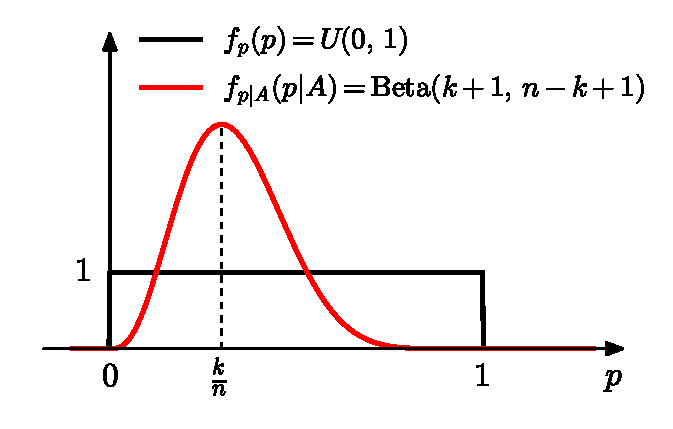
\includegraphics[width=\textwidth]{figuras/flip_coin_posterior_probability.pdf}
  \end{minipage}\hfill
  \begin{minipage}[c]{0.45\textwidth}
    \caption{
       Densidad \(f_p(p)\) a priori y densidad \(f_{p|A}(p|A)\) a posteriori. Luego de haber realizado el experimento \(n\) veces, los resultados se reflejan en la densidad a posteriori. En el ejemplo de la figura, \(n=10\) y \(k=3\). La densidad a posteriori es \(\beta(n,\,k)\), cuyo máximo se da en \(k/n\).
    } \label{fig:flip_coin_posterior_probability}
  \end{minipage}
\end{figure}

La densidad de probabilidad a posteriori puede ser empleada para realizar predicciones en nuevos experimentos. Por ejemplo, teniendo en cuenta el resultado del experimento anterior, puede calcularse la probabilidad de que salga cara en la tirada \(n+1\). Sea el evento \(B\)=``sale cara en la tirada \(n+1\) dado que \(k\) caras salieron en las \(n\) tiradas anteriores''. Del teorema de la probabilidad total dado por la ecuación \ref{eq:total_probability_theorem_continuous} se tiene que
\[
 P(B)=\int_{-\infty}^{\infty}P\{B|\p = p\}f_{p|A}(p|A)\,dp.
\]
Notar que a diferencia de la ecuación \ref{eq:total_probability_theorem_continuous} se usó la densidad de probabilidad a posteriori de forma de reflejar el conocimiento adquirido en el experimento realizado previamente. Teniendo en cuenta que \(P(B|\p=p)=p\), y usando de valor calculado antes de la densidad condicional, se llega a que
\begin{align*}
 P(B)&=\int_{-\infty}^{\infty}p\frac{(n+1)!}{(n-k)!k!}p^k(1-p)^{n-k}\,dp\\
     &=\frac{(n+1)!}{(n-k)!k!}\int_{-\infty}^{\infty}p^{k+1}(1-p)^{n-k}\,dp.
\end{align*}
La última integral puede calcularse de forma análoga a la calculada previamente. Aplicando integración por partes \(k+1\) veces, puede verse que
\[
 \int_{-\infty}^{\infty}p^{k+1}(1-p)^{n-k}\,dp=\frac{(n-k)!(k+1)!}{(n+2)!},
\]
y por lo tanto, al sustituir el resultado en la ecuación anterior, se llega a que
\[
 P(B)=\frac{k+1}{n+2}.
\]
Por ejemplo, si en \(n=10\) tiradas salieron \(k=5\) caras, la probabilidad que en la onceava tirada salga cara es \(P(B)=6/12=0.5\).

\chapter{Funciones de una variable aleatoria}

Esta sección sigue lo explicado en el capítulo 5 de \cite{papoulis2002probability}.

\section{\texorpdfstring{Distribución de \(\y=g(\x)\)}{}}

Sean \(\x\) e \(\y\) dos variables aleatorias tal que \(\y=g(\x)\), con \(g(x)\) una función de variable real \(x\). Es de interés expresar la distribución de probabilidad \(F_y(y)\) de la variable aleatoria \(\y\) en términos de la distribución de probabilidad \(F_x(x)\) de la variable aleatoria \(\x\) y la función \(g(x)\). Para hacerlo, hay que determinar el conjunto \(R_y\) de valores de \(x\) tal que \(g(x)<y\), y la probabilidad de que \(\x\) esté en ese conjunto.

\subsection{\texorpdfstring{Ejemplo 5-1: Distribución de \(\y=a\x+b\)}{}}\label{sec:y_equals_ax_plus_b_distribution}

Sea
\[
 \y=a\x+b.
\]
Para determinar \(F_y(y)\) hay que encontrar los valores de \(x\) de forma que \(ax+b\leq y\). Se consideran dos casos en función de si \(a\) es mayor o menor que cero.
\begin{itemize}
 \item \(a>0\): \(ax+b\leq y\) si \(x\leq(y-b)/a\) y por lo tanto
 \[
  F_y(y)=P\left\{x\leq\frac{y-b}{a}\right\}=F_x\left(\frac{y-b}{a}\right), \qquad a>0.
 \]
 \item \(a<0\): \(ax+b\leq y\) si \(x\geq(y-b)/a\) y por lo tanto
 \[
  F_y(y)=P\left\{x\geq\frac{y-b}{a}\right\}=1-F_x\left(\frac{y-b}{a}\right), \qquad a<0.
 \]
\end{itemize}
Para obtener la densidad de probabilidad \(f_y(y)\), se diferencia \(F_y(y)\), por lo que
\begin{itemize}
 \item \(a>0\): 
 \[
  f_y(y)=\frac{1}{a}f_x\left(\frac{y-b}{a}\right), \qquad a>0.
 \]
 \item \(a<0\): 
 \[
  f_y(y)=-\frac{1}{a}f_x\left(\frac{y-b}{a}\right), \qquad a<0,
 \]
\end{itemize}
que se puede escribir en una ecuación para todo \(a\) como
\begin{equation}\label{eq:y_equals_ax_plus_b_density}
 f_y(y)=\frac{1}{|a|}f_x\left(\frac{y-b}{a}\right).
\end{equation}

\subsection{\texorpdfstring{Ejemplo 5-2: Distribución de \(\y=\x^2\)}{}}\label{sec:x_square_distribution}

Considérese el caso en que
\[
 \y=\x^2
\]
y se quiere determinar \(F_y(y)=P\{\y\leq y\}=P\{\x^2\leq y\}\)
\begin{itemize}
 \item Si \(y\geq 0\), se cumple que \(x^2\leq y\) si \(-\sqrt{y}\leq x\leq \sqrt{y}\) y por lo tanto
 \[
  F_y(y)=P\{-\sqrt{y}\leq \x\leq \sqrt{y}\}=F_x(\sqrt{y})-F_x(-\sqrt{y}), \qquad y\geq0.
 \]
 \item Si \(y<0\), no hay valores de \(x\) tal que \(x^2\leq y\) y por lo tanto
 \[
  F_y(y)=P\{\emptyset\}=0,\qquad y<0.
 \]
\end{itemize}
La densidad de probabilidad \(f_y(y)\) puede obtenerse diferenciando \(F_y(y)\), y queda
\[
\def\arraystretch{2.0}
 f_y(y)=
 \left\{\begin{array}{ll}
  \dfrac{1}{2\sqrt{y}}\left(f_x(\sqrt{y})+f_x(-\sqrt{y})\right), & y\geq 0\\
  0, & \textrm{en otro caso}
 \end{array}, \right.
\]
En el caso en que \(f_x(x)\) es una función par, es decir, \(f_x(x)=f_x(-x)\), la ecuación anterior se reduce a
\begin{equation}\label{eq:rv_y_equal_x_square_density_even}
 f_y(y)=\frac{1}{\sqrt{y}}f_x(\sqrt{y})U(y),
\end{equation}
donde \(U(x)\) es la función escalón de Heaviside. En particular, si \(\x\sim N(0,\,1)\) y por lo  tanto
\[
 f_x(x)=\frac{1}{\sqrt{2\pi}}e^{-x^2/2},
\]
sustituyendo en la ecuación \ref{eq:rv_y_equal_x_square_density_even}, se obtiene que la distribución de la variable aleatoria \(\y=\x^2\) es
\begin{equation}\label{eq:rv_x_square_normal_density}
 f_y(y)=\frac{1}{\sqrt{2\pi y}}e^{-y/2}U(y).
\end{equation}
Por otro lado, la densidad de probabilidad de una variable aleatoria chi-cuadrado con \(n=1\) grado de libertad es (ecuación \ref{eq:pdf_chi_square})
\[
 f_z(z)=\frac{z^{-1/2}}{2^{1/2}\,\Gamma(1/2)} e^{z/2}U(x)=\frac{1}{\sqrt{2z}\,\Gamma(1/2)} e^{z/2}U(z)
\]
y que con la función \(\Gamma(\alpha)\) definida por la ecuación \ref{eq:gamma_function}, \(\Gamma(1/2)\) es  
\begin{align*}
 \Gamma(1/2)&=\int_{0}^{-\infty}z^{-1/2}e^{-z}\,dz\\
    &=\int_{0}^{\infty}\frac{e^{-z}}{\sqrt{x}}\,dz\\
    &\overset{(a)}{=}2\int_{0}^{\infty}e^{-u^2}\,du\\
    &=\int_{-\infty}^{\infty}e^{-u^2}\,du\\
    &\overset{(b)}{=}\sqrt{\pi},
\end{align*}
donde en \((a)\) se realizó el cambio de variable \(u=\sqrt{z}\), por lo que \(du=dz/(2\sqrt{z})\), y en \((b)\) se notó que la integral es gaussiana (ecuación \ref{eq:random_gaussian_integral}). Por lo tanto, si \(\z\sim\chi^2(1)\), entonces
\[
 f_z(z)=\frac{1}{\sqrt{2\pi z}} e^{z/2}U(z).
\]
Como esta distribución coincide con la ecuación \ref{eq:rv_x_square_normal_density}, se concluye que si \(\x\sim N(0,\,1)\), entonces \(\y=\x^2\sim\chi^2(1)\).

\section{\texorpdfstring{Densidad de \(\y=g(\x)\)}{}}

La determinación de la densidad de probabilidad de \(\y=g(\x)\) en función de \(f_x(x)\) y \(g(x)\) está dada por el \emph{teorema fundamental}, que se plantea como sigue.

\subsection{Teorema fundamental}\label{sec:fundamental_theorem}

Para calcular \(f_y(y)\) para un valor específico de \(y\), se resuelve la ecuación \(y=g(x)\). Sean \(x_n\) las raíces reales de dicha ecuación, es decir,
\[
 y=g(x_1)=\dots=g(x_n)=\dots
\]
El teorema fundamental indica que la densidad de probabilidad \(f_y(y)\) para ese valor de \(y\) es
\begin{equation}\label{eq:functions_of_rv_fundamental_theorem}
 f_y(y)=\frac{f_x(x_1)}{\left|g'(x_1)\right|}+\cdots+\frac{f_x(x_n)}{\left|g'(x_n)\right|}+\cdots
\end{equation}
Para demostrarlo, se considera que la ecuación \(y=g(x)\) tiene tres raíces sin perder generalidad, como se muestra en la figura \ref{fig:fy_as_function_of_fx}. Como indica la ecuación \ref{eq:density_definition_as_probability}, se cumple que
\[
 f_y(y)=P\{y<\y\leq y+dy\}.
\]
Como \(\y=g(\x)\), hay que encontrar el conjunto de valores de \(x\) que cumplen que \(y<g(x)\leq y+dy\) y calcular la  probabilidad de que \(\x\) esté en dicho conjunto. Observando la figura \ref{fig:fy_as_function_of_fx}, ese conjunto consiste en los tres intervalos
\[
 x_1<x\leq x_1+dx_1,\qquad x_2+dx_2\leq x<x_2,\qquad x_3<x\leq x_3+dx_3, 
\]
con \(dx_1>0\) y \(dx_3>0\) pero \(dx_2<0\). Por lo tanto, se cumple que
\begin{align*}
 P\{y<\y\leq y+dy\}=&P\{x_1<x\leq x_1+dx_1\}\\
    &+P\{x_2+dx_2\leq x<x_2\}+P\{x_3<x\leq x_3+dx_3\}.
\end{align*}
El lado derecho de la igualdad es el área sombreada en la figura \ref{fig:fy_as_function_of_fx}. Como
\[\arraycolsep=1.4pt\def\arraystretch{1.4}
 \begin{array}{lllp{1cm}lll}
   P\{x_1<x\leq x_1+dx_1\}&=&f_x(x_1)dx_1&  &dx_1&=&dy/g'(x_1)\\
   P\{x_2+dx_2\leq x<x_2\}&=&f_x(x_2)|dx_2|&  &dx_2&=&dy/g'(x_2)\\
   P\{x_3<x\leq x_3+dx_3\}&=&f_x(x_3)dx_3&  &dx_3&=&dy/g'(x_3),
 \end{array}
\]
sustituyendo estos resultados en la ecuación anterior, se concluye que
\[
 f_y(y)dy=\frac{f_x(x_1)}{g'(x_1)}dy+\frac{f_x(x_2)}{|g'(x_2)|}dy+\frac{f_x(x_3)}{g'(x_3)}dy,
\]
lo que resulta en la ecuación \ref{eq:functions_of_rv_fundamental_theorem}.
\begin{figure}[!htb]
\begin{center}
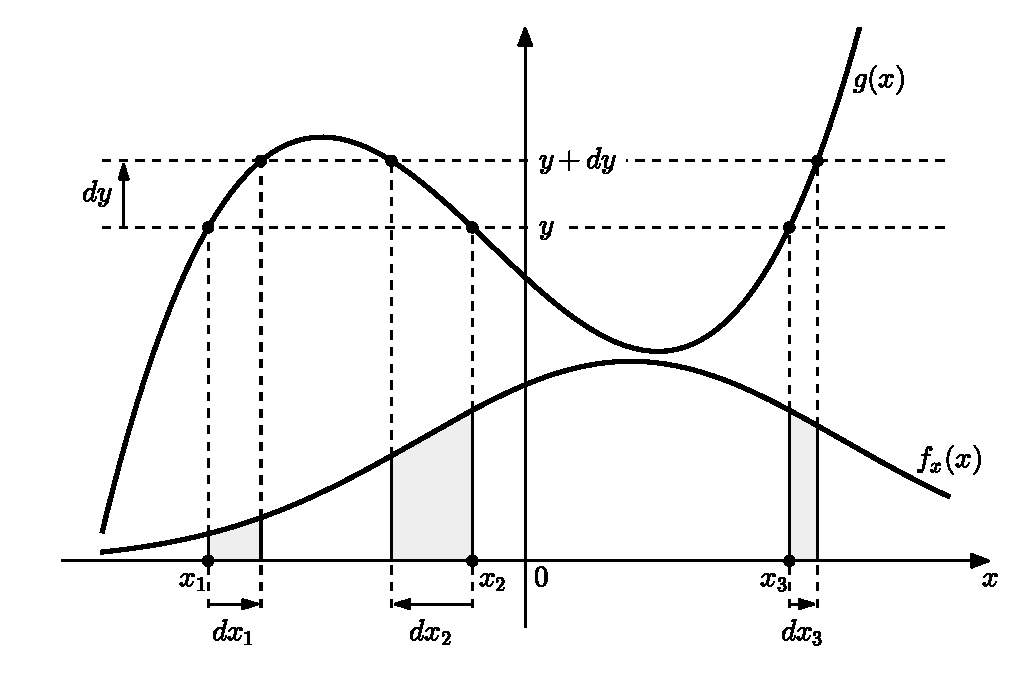
\includegraphics[width=0.8\columnwidth]{figuras/fy_as_function_of_fx.pdf}
\caption{\label{fig:fy_as_function_of_fx} Teorema fundamental. Se grafica la función \(g(x)\) y la densidad de probabilidad \(f_x(x)\). La ecuación \(g(x)=y\) tiene raíces \(x_1\), \(x_2\) y \(x_3\) y la ecuación \(g(x)=y+dy\) tiene raíces \(x_1+dx_1\), \(x_2+dx_2\) y \(x_3+dx_3\). Por lo tanto, \(P\{y<\y\leq y+dy\}\) corresponde a la probabilidad de que \(x\) esté en los intervalos \((x_1,\,x_1+dx_1)\), \((x_2+dx_2,\,x_2)\) y \((x_3,\,x_3+dx_3)\) y es el área sombreada.}
\end{center}
\end{figure}

A continuación se considera una aplicación que tiene cierta dificultad.

\subsection{Ejemplo}

Se quiere determinar \(f_y(y)\) en el caso en que
\[
 \y=a\sin(\x+\theta), \qquad a>0.
\]
Si \(|y|>a\), la ecuación \(y=a\sin(x+\theta)\) no tiene soluciones, y por lo tanto \(f_y(y)=0\). Si \(|y|<a\), resolviendo la ecuación \(y=a\sin(x+\theta)\) se tiene que
\begin{align*}
 y=a\sin(x+\theta)\quad\Leftrightarrow\quad &
 \left\{\begin{array}{ll}
  y=a\sin(x+\theta+2k\pi) & \textrm{o}\\
  y=a\sin(\pi-x-\theta+2k\pi) & 
 \end{array}\right.\\
 \quad\Leftrightarrow\quad &
 \left\{\begin{array}{ll}
  x+\theta+2k\pi=\arcsin(y/a) & \textrm{o}\\
  \pi-x-\theta+2k\pi=\arcsin(y/a) & 
 \end{array}\right.\\
 \quad\Leftrightarrow\quad &
 \left\{\begin{array}{ll}
  x=\arcsin(y/a)-\theta+2k\pi & \textrm{o}\\
  x=\pi-\arcsin(y/a)-\theta+2k\pi & 
 \end{array}\right.\\
 \quad\Leftrightarrow\quad &
 \left\{\begin{array}{ll}
  x=\arcsin(y/a)-\theta+2k\pi & \textrm{o}\\
  x=-\arcsin(y/a)-\theta+(2k+1)\pi & 
 \end{array}\right.
\end{align*}
Este resultado puede expresarse en una única ecuación como
\begin{equation}\label{eq:functions_of_rv_arcsin}
 x_n=(-1)^n\arcsin\left(\frac{y}{a}\right)-\theta+n\pi,\qquad n=\dots,-2,\,-1,\,0,\,1,\,2,\dots
\end{equation}
es decir, si \(|y|<a\) hay infinitas soluciones \(y=g(x_n)=a\sin(x_n+\theta)\). En la figura \ref{fig:fy_with_y_sin_x} se ilustra la deducción de las soluciones.
\begin{figure}[!htb]
\begin{center}
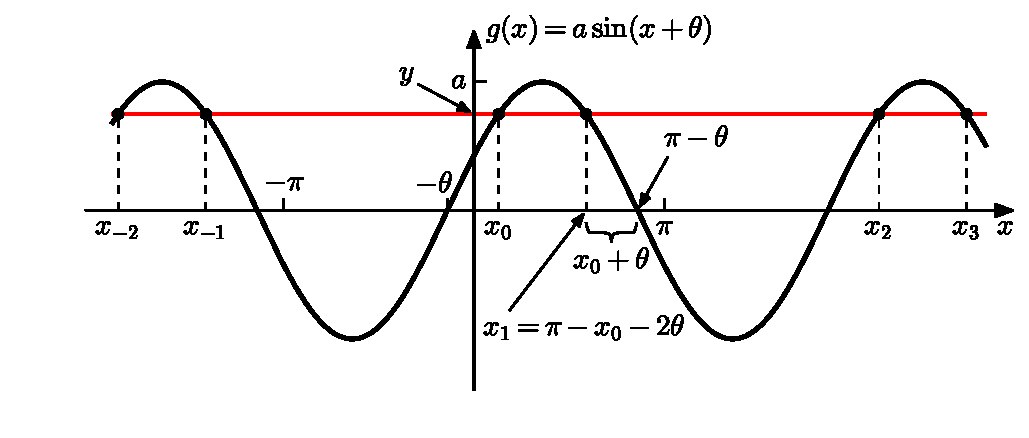
\includegraphics[width=0.8\columnwidth]{figuras/fy_with_y_sin_x.pdf}
\caption{\label{fig:fy_with_y_sin_x} Soluciones de \(y=a\sin(x+\theta)\) cuando \(|y|<a\). Si \(x_0\) es solución, también son raíces los valores \(x_0+2k\pi\). Estas raíces son de la forma \(x=\arcsin(y/a)-\theta+2k\pi\). Además, también es solución el valor \(x_1=(\pi-\theta)-(x_0+\theta)=\pi-x_0-2\theta\) y todos los valores que distan \(2k\pi\) de este, \(x_1+2k\pi\). Estas raíces son de la forma \(x=-\arcsin(y/a)-\theta+(2k+1)\pi\).}
\end{center}
\end{figure}

Por otro lado, se tiene que
\begin{align*}
 g'(x_n)&=a\cos(x_n+\theta)\\
        &\overset{(a)}{=}\sqrt{a^2-a^2\sin^2(x_n+\theta)}\\
        &=\sqrt{a^2-y^2},
\end{align*}
donde en \((a)\) se empleó la propiedad trigonométrica \(\sin^2x+\cos^2x=1\).
Sustituyendo estos resultados en la ecuación \ref{eq:functions_of_rv_fundamental_theorem}, se llega a que
\begin{equation}\label{eq:functions_of_rv_arcsin_f_y}
 f_y(y)=\frac{1}{\sqrt{a^2-y^2}}\sum_{n=-\infty}^{\infty}f_x(x_n),\qquad |y|<a,
\end{equation}
con \(x_n\) dado por la ecuación \ref{eq:functions_of_rv_arcsin}.

\emph{Caso particular:} considérese el caso en que \(\x\) es uniforme en el intervalo \((-\pi,\,\pi)\). La ecuación \(y=a\sin(x+\theta)\) tiene únicamente dos raíces el intervalo \((-\pi,\,\pi)\) para cualquier valor de \(\theta\). En la figura \ref{fig:fy_with_y_sin_x} estas raíces son \(x_0\) y \(x_1\). La función \(f_x(x)\) vale \(1/2\pi\) para esas dos raíces y 0 para las raíces fuera del intervalo \((-\pi,\,\pi)\). Por lo tanto, la sumatoria de la ecuación \ref{eq:functions_of_rv_arcsin_f_y} tiene solo dos sumandos no nulos de valor \(1/2\pi\) resultando en
\[
 f_y(y)=\frac{1}{\pi\sqrt{a^2-y^2}},\qquad |y|<a.
\]

Para calcular la distribución de probabilidad \(F_y(y)\), se observa que \(\y<y\) si \(\x\) está en el intervalo \((-\pi,\, x_0)\) o \((x_1,\,\pi)\), como se ve en la figura \ref{fig:fy_with_y_sin_x}. El primer intervalo tiene una longitud de \(x_0+\pi\) y el segundo intervalo tiene una longitud de
\[
 \pi-x_1=\pi-(\pi-x_0-2\theta)=x_0+2\theta,
\]
por lo que la suma de los largos de ambos intervalos es
\begin{align*}
 (x_0+\pi)+(x_0+2\theta)&=\pi+2x_0+2\theta\\
  &\overset{(a)}{=}\pi+2\left[\arcsin\left(\frac{y}{a}\right)-\theta\right]+2\theta\\
  &=\pi+2\arcsin\left(\frac{y}{a}\right),
\end{align*}
donde en \((a)\) se sustituyó \(x_0\) usando la ecuación \ref{eq:functions_of_rv_arcsin} con \(n=0\). Este resultado es el intervalo correspondiente al evento \(\{\y<y\}\). Dividiendo entre el largo total del intervalo \((-\pi,\,\pi)\), que es \(2\pi\), se obtiene la distribución de probabilidad (casos favorables sobre casos posibles),
\[
 F_y(y)=P\{\y<y\}=\frac{1}{2}+\frac{1}{\pi}\arcsin\left(\frac{y}{a}\right).
\]

\section{Media y varianza}

\subsection{Definiciones}\label{sec:median_variance_definition}

\newcolumntype{Y}{>{\centering\arraybackslash}X}
\begin{tabularx}{\textwidth}{YY} 
\multicolumn{2}{c}{\textbf{Media} (\(\eta\))}\\
\(\x\) variable aleatoria continua & \(\x\) variable aleatoria discreta\\
\\
\(\displaystyle E\{\x\}=\int_{-\infty}^{\infty}xf(x)\,dx\) & \(\displaystyle E\{\x\}=\sum_{i}x_iP\{\x=x_i\}\)\\ 
\multicolumn{2}{c}{\textbf{Media condicional}}\\
\(\x\) variable aleatoria continua & \(\x\) variable aleatoria discreta\\
\\
\(\displaystyle E\{\x|M\}=\int_{-\infty}^{\infty}xf(x|M)\,dx\) & \(\displaystyle E\{\x|M\}=\sum_{i}x_iP\{\x=x_i|M\}\)\\ 
\multicolumn{2}{c}{\textbf{Media de} \(\mathbf{g(x)}\)}\\
\(\x\) variable aleatoria continua & \(\x\) variable aleatoria discreta\\
\\
\(\displaystyle E\{g(\x)\}=\int_{-\infty}^{\infty}g(x)f_x(x)\,dx\) & \(\displaystyle E\{g(\x)\}=\sum_{i}g(x_i)P\{\x=x_i\}\)\\ 
\multicolumn{2}{c}{\textbf{Varianza} (\(\sigma^2 \triangleq E\{(\x-\eta)^2\}\))}\\
\(\x\) variable aleatoria continua & \(\x\) variable aleatoria discreta\\
\\
\(\displaystyle \sigma^2=\int_{-\infty}^{\infty}(x-\eta)^2f(x)\,dx\) & \(\displaystyle \sigma^2=\sum_{i}(x_i-\eta)^2P\{\x=x_i\}\)
\end{tabularx}
\vspace{0.2cm}

Algunas observaciones son las siguientes:
\paragraph{Media de \(g(x)\)} Arriba se indicó que
\begin{equation}\label{eq:mean_of_gx}
 E\{g(\x)\}=\int_{-\infty}^{\infty}g(x)f_x(x)dx.
\end{equation}
Esto en realidad no es una definición, sino que debe ser demostrado. Sea la variable aleatoria \(\y=g(\x)\) construida a partir de una variable aleatoria \(\x\) y una función \(g(x)\). Por definición, la media de \(\y\) es
\begin{equation}\label{eq:mean_of_y}
 E\{\y\}=\int_{-\infty}^{\infty}yf_y(y)\,dy.
\end{equation}
Supóngase que para cierto valor de \(y\), la función \(g(x)\) tiene tres raíces \(x_1\), \(x_2\) y \(x_3\), es decir, \(y=g(x_1)=g(x_2)=g(x_3)\), como en la figura \ref{fig:fy_as_function_of_fx}. Como se vio en la sección \ref{sec:fundamental_theorem}, se cumple que\footnote{En esta demostración, a diferencia de la demostración de la sección \ref{sec:fundamental_theorem}, se consideran todos los \(dx_i\) positivos}
\[
 f_y(y)dy=f_x(x_1)dx_1+f_x(x_2)dx_2+f_x(x_3)dx_3.
\]
Multiplicando por \(y\) se tiene que
\[
 yf_y(y)dy=g(x_1)f_x(x_1)dx_1+g(x_2)f_x(x_2)dx_2+g(x_3)f_x(x_3)dx_3.
\]
Por lo tanto, a cada diferencial en la ecuación \ref{eq:mean_of_y}, corresponde uno o mas diferenciales en la ecuación \ref{eq:mean_of_gx}. Como \(dy\) abarca todo el eje \(y\), los \(dx\) correspondientes abarcan todo el eje \(x\) y no se solapan, las ecuaciones \ref{eq:mean_of_gx} y \ref{eq:mean_of_y} son equivalentes. Notar que entonces, para calcular la media de \(\y=g(\x)\) no es necesario conocer la densidad de probabilidad \(f_y(y)\) de \(\y\).

\paragraph{Varianza} Debido a que la esperanza es lineal (ecuación \ref{eq:mean_linearity} mas adelante), la varianza puede expresarse como
\begin{align}\label{eq:variance_definition1}
 \sigma^2&\triangleq E\{(\x-\eta)^2\}\\
   &=E\{\x^2-2\x\eta+\eta^2\}\nonumber\\
   &=E\{\x^2\}-2\eta E\{\x\}+\eta^2\nonumber\\
   &=E\{\x^2\}-\eta^2,\nonumber
\end{align}
es decir,
\begin{equation}\label{eq:variance_definition2}
 \sigma^2=E\{\x^2\}-E^2\{\x\}.
\end{equation}
\emph{Transformación lineal}: la varianza de la variable aleatoria \(\y=a\x+b\), donde \(\x\) es una variable aleatoria de media \(\eta_x\) y varianza \(\sigma_x^2\) es
\begin{align}\label{eq:variance_linear_transform}
 \sigma_y^2&\triangleq E\{(\y-\eta_y)^2\}\nonumber\\
   &\overset{(a)}{=}E\{[(a\x+b)-(a\eta_x+b)]^2\}\nonumber\\
   &=E\{[a(\x-\eta_x)]^2\}\nonumber\\
   &=E\{a^2(\x-\eta_x)^2\}\nonumber\\
   &\overset{(b)}{=}a^2E\{(\x-\eta_x)^2\}\nonumber\\
   &=a^2\sigma_x^2,
\end{align}
donde en \((a)\) se empleó que \(\eta_y=a\eta_x+b\) y en \((b)\) se empleó la propiedad de linealidad de la esperanza.

\subsection{Media en función de la distribución}

Sea una variable aleatoria \(\x\) con distribución de probabilidad \(F(x)\). Se divide el eje \(x\) en intervalos \((x_k,\,x_{k+1})\) de largo \(\Delta x\) como se muestra en la figura \ref{fig:mean_and_distribution}. En la figura, se observa que el área de cada región diferencial rectangular es \(x_k[F(x_{k+1})-F(x_k)]=x_k[F(x_k+\Delta x)-F(x_k)]\). Además, se cumple que
\[
 F(x_k+\Delta x)-F(x_k)=P\{x_k<\x<x_k+\Delta x\}\approx f(x_k)\Delta x.
\]
Por lo tanto, la suma de todas las regiones diferenciales rectangulares es
\[
 \sum_k x_k[F(x_k+\Delta x)-F(x_k)]\approx \sum_k x_kf(x_k)\Delta x \to \int_{-\infty}^{\infty} xf(x)\,dx=E\{\x\}
\]
cuando \(\Delta x \to 0\). Notando que las regiones rectangulares correspondientes a \(x_k\) negativos contribuyen con áreas negativas, se concluye que
\[
 E\{\x\}=(1BD)-(0AB),
\]
donde \((1BD)\) y \((0AB)\) son las áreas coloreadas en la figura \ref{fig:mean_and_distribution}. Por lo tanto,
\[
 E\{\x\}=\int_{0}^{\infty}[1-F(x)]\,dx-\int_{-\infty}^{0}F(x)\,dx.
\]
Como caso particular, si una variable aleatoria toma solo valores positivos, se cumple que
\[
 E\{\x\}=\int_{0}^{\infty}[1-F(x)]\,dx.
\]
\begin{figure}[!htb]
\begin{center}
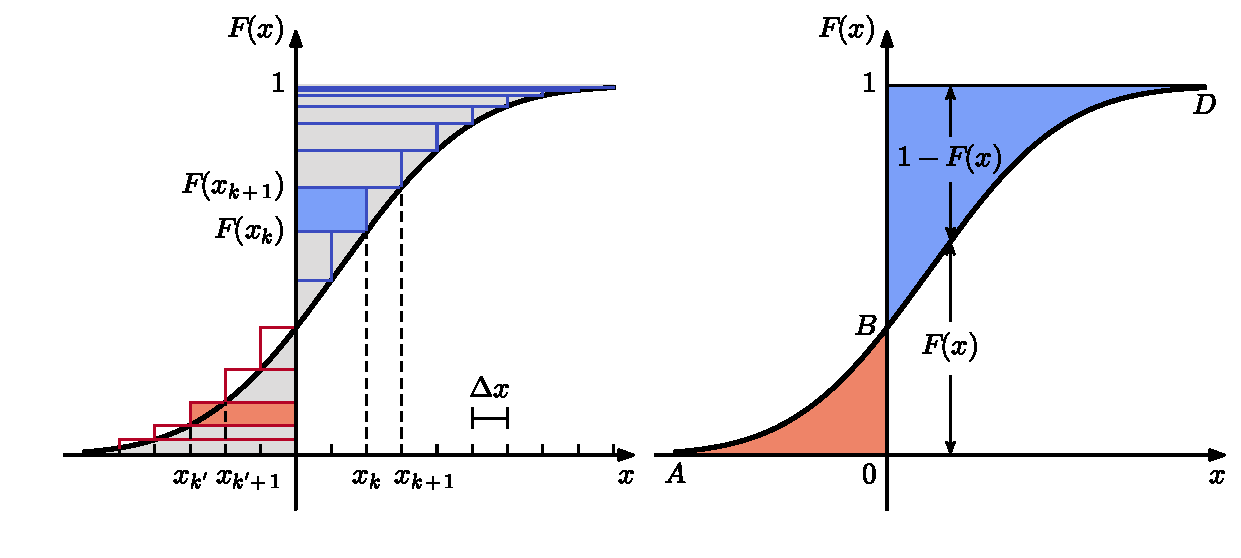
\includegraphics[width=1\columnwidth]{figuras/mean_and_distribution.pdf}
\caption{\label{fig:mean_and_distribution} Deducción de la media de \(\x\) en función de la ditribución de probabilidad. La media de \(\x\) esta dada por \((1BD)-(0AB)\), donde \((1BD)\) y \((0AB)\) son las áreas coloreadas en la figura de la derecha.}
\end{center}
\end{figure}

\subsection{Ejemplo 5-18} Se quiere calcular \(E\{\x|M\}\) con \(M=\{x\geq a\}\). A partir de la definición, se tiene que
\[
 E\{\x|\x\geq a\}=\int_{-\infty}^{\infty}xf(x|\x\geq a)\,dx.
\]
Para determinar \(f(x|\x\geq a)\) hay que determinar primero \(F(x|\x\geq a)\) de forma similar a como se realizó en la sección \ref{sec:conditional_distributions} usando la definición dada por la ecuación \ref{eq:conditional_distribution_definition},
\[
 F(x|\x\geq a)=P\{\x\leq x|\x\geq a\}=\frac{P\{\x\leq x,\,\x\geq a\}}{P\{\x\geq a\}},
\]
\begin{itemize}
  \item Si \(x<a\), se cumple que \(\{\x\leq x,\,\x\geq a\}=\{\emptyset\}\) y como \(P\{\emptyset\}=0\) se tiene que,
 \[
  F(x|\x\geq a)=0,\qquad x<a.
 \]
 \item Si \(x\geq a\), se cumple que \(\{\x\leq x,\,\x\geq a\}=\{a\leq \x\leq x\}\) y por lo tanto,
 \[
  F(x|\x\geq a)=\frac{P\{a\leq \x\leq x\}}{P\{\x\geq a\}}=\frac{F(x)-F(a)}{1-F(a)},\qquad x\geq a.
 \]
\end{itemize}
Derivando respecto a \(x\), se obtiene la densidad condicional, que es
\[
   f(x|\x\geq a)=
 \left\{\begin{array}{ll}
  0, & x<a \\
  \\
  \dfrac{f(x)}{1-F(a)}=\dfrac{f(x)}{\int_{a}^{\infty}f(x)\,dx}, & x\geq a.
 \end{array} \right.
\]
Por lo tanto, se concluye que
\[
 E\{\x|\x\geq a\}=\frac{\int_{a}^{\infty}xf(x)\,dx}{\int_{a}^{\infty}f(x)\,dx}.
\]

\subsection{Media y varianza de una variable aleatoria normal}\label{sec:normal_mean_and_variance}

Una variable aleatoria normal tiene densidad de probabilidad (ecuación \ref{eq:pdf_gaussian})
\[
 f_x(x)=\frac{1}{\sqrt{2\pi\sigma^2}}e^{-(x-\eta)^2/2\sigma^2}.
\]
Se verá a continuación que las constantes \(\eta\) y \(\sigma^2\) son la media y la varianza respectivamente. Para esto, hay que demostrar que
\[
 E\{\x\}=\frac{1}{\sqrt{2\pi\sigma^2}}\int_{-\infty}^{\infty}xe^{-(x-\eta)^2/2\sigma^2}\,dx=\eta
\]
\[
 E\{(\x-\eta)^2\}=\frac{1}{\sqrt{2\pi\sigma^2}}\int_{-\infty}^{\infty}(x-\eta)^2e^{-(x-\eta)^2/2\sigma^2}\,dx=\sigma^2.
\]
Hay varias formas de hacerlo. Una de ellas es resolver las integrales usando métodos de integración convencionales. Otras formas explotan las propiedades de la densidad de probabilidad y de la esperanza. 

Se comenzará realizando la demostración resolviendo las integrales de forma convencional. En el caso de la media, se tiene que
\begin{align*}
 E\{\x\}&=\frac{1}{\sqrt{2\pi\sigma^2}}\int_{-\infty}^{\infty}xe^{-(x-\eta)^2/2\sigma^2}\,dx\\
    &\overset{(a)}{=}\frac{1}{\sqrt{2\pi\sigma^2}}\int_{-\infty}^{\infty}(\sigma z+\eta)e^{-z^2/2}\sigma\,dz\\
    &=\frac{1}{\sqrt{2\pi}}\left(\sigma\int_{-\infty}^{\infty}ze^{-z^2/2}\,dz+\eta\int_{-\infty}^{\infty}e^{-z^2/2}\,dz\right)\\
    &\overset{(b)}{=}\frac{1}{\sqrt{2\pi}}\left(\sigma\cdot 0+\eta\cdot \sqrt{2\pi}\right)\\
    &=\eta,
\end{align*}
donde en \((a)\) se realizó el cambio de variable \(z=(x-\eta)/\sigma\), por lo  que \(\sigma dz=dx\), y en \((b)\) se observó que el integrando de la primera integral es una función impar por lo que integra a cero, y la segunda integral es gaussiana como la  de la ecuación \ref{eq:random_gaussian_integral_with_sigma} con \(\sigma^2=1\), por lo que integra a \(\sqrt{2\pi}\). Para el cálculo de la varianza, se ve que
\begin{align*}
 E\{(\x-\eta)^2\}&=\frac{1}{\sqrt{2\pi\sigma^2}}\int_{-\infty}^{\infty}(x-\eta)^2e^{-(x-\eta)^2/2\sigma^2}\,dx\\
 &\overset{(a)}{=}\frac{1}{\sqrt{2\pi\sigma^2}}\int_{-\infty}^{\infty}\sigma^3z^2e^{-z^2/2}\,dz\\
 &\overset{(b)}{=}\frac{\sigma^2}{\sqrt{2\pi}}\left(-ze^{-z^2/2}\bigg|_{-\infty}^{\infty}  +\int_{-\infty}^{\infty}e^{-z^2/2}\,dz\right)\\
 &\overset{(c)}{=}\frac{\sigma^2}{\sqrt{2\pi}}\left(0+\sqrt{2\pi}\right)\\
 &=\sigma^2,
\end{align*}
donde en \((a)\) se realizó el cambio de variable \(z=(x-\eta)/\sigma\) igual que antes, en \((b)\) se aplicó integración por partes, \(\int udv=uv-\int vdu\), con \(u=z\) y \(dv=ze^{-z^2/2}\) por lo que \(du=1\) y \(v=-e^{-z^2/2}\), y en \((c)\) se observó que el primer término es nulo debido a que la velocidad de convergencia de \(e^{-z^2/2}\to0\) es mayor que la de \(z\to\infty\), y la segunda integral coincide con la de la ecuación \ref{eq:random_gaussian_integral_with_sigma} con \(\sigma^2=1\), por lo que integra a \(\sqrt{2\pi}\).

Otra forma de realizar el mismo cálculo es la siguiente. Debido a que \(f(x)\) es una densidad de probabilidad, se cumple que
\begin{equation}\label{eq:functions_of_normal_mean_variance_derivation}
 \frac{1}{\sqrt{2\pi\sigma^2}}\int_{-\infty}^{\infty}e^{-(x-\eta)^2/2\sigma^2}\,dx=1
 \quad\Leftrightarrow\quad
 \int_{-\infty}^{\infty}e^{-(x-\eta)^2/2\sigma^2}\,dx=\sigma\sqrt{2\pi}.
\end{equation}
Esto además, para el caso particular de una distribución gaussiana, se demostró en la sección \ref{sec:continuous_random_variables}. Para calcular la media, se diferencia la ecuación anterior respecto a \(\eta\). Esto resulta en
\[
\begin{array}{*4{>{\displaystyle}l}}
  \int_{-\infty}^{\infty}\frac{(x-\eta)}{\sigma^2}e^{-(x-\eta)^2/2\sigma^2}\,dx&=&0&\Rightarrow\\
  \int_{-\infty}^{\infty}xe^{-(x-\eta)^2/2\sigma^2}\,dx&=&\eta\int_{-\infty}^{\infty}e^{-(x-\eta)^2/2\sigma^2}\,dx&\Rightarrow\\
  \int_{-\infty}^{\infty}xe^{-(x-\eta)^2/2\sigma^2}\,dx&=&\eta\sqrt{2\pi\sigma^2}&\Rightarrow\\
  \frac{1}{\sqrt{2\pi\sigma^2}}\int_{-\infty}^{\infty}xe^{-(x-\eta)^2/2\sigma^2}\,dx&=&\eta,&
\end{array}
\]
que es lo que se quería demostrar. Para calcular la varianza, se diferencia la ecuación \ref{eq:functions_of_normal_mean_variance_derivation} respecto a \(\sigma\). De esta forma, se tiene que
\[
\begin{array}{*4{>{\displaystyle}l}}
  \int_{-\infty}^{\infty}\frac{(x-\eta)^2}{\sigma^3}e^{-(x-\eta)^2/2\sigma^2}\,dx&=&\sqrt{2\pi}&\Rightarrow\\
  \frac{1}{\sqrt{2\pi\sigma^2}}\int_{-\infty}^{\infty}(x-\eta)^2e^{-(x-\eta)^2/2\sigma^2}\,dx&=&\sigma^2,&
\end{array}
\]
que es lo que se quería demostrar.

\subsection{Media y varianza de una variable aleatoria Bernoulli}\label{sec:bernoulli_rv_mean_variance}

Como se definió en la sección \ref{sec:discrete_random_variables}, una variable aleatoria Bernoulli \(\x\) toma valores 1 y 0 con probabilidades \(p\) y \(q=1-p\) respectivamente, es decir,
\[
 P\{\x=1\}=p,\qquad\qquad P\{\x=0\}=q=1-p.
\]
Por lo tanto,
\[
 E\{\x\}=\sum_{i}x_iP\{\x=x_i\}=1\times p+0\times q=p
\]
\[
 E\{\x^2\}=\sum_{i}x_i^2P\{\x=x_i\}=1^2\times p+0^2\times q=p.
\]
Además,
\[
 \sigma^2=E\{\x^2\}-E^2\{\x\}=p-p^2=p(1-p)=pq.
\]

\subsection{Ejemplo: media y mediana}

Mediante el siguiente ejemplo, se pretende clarificar los conceptos de media y mediana. Se considera la variable aleatoria \(\x\) con densidad de probabilidad 
\[\def\arraystretch{1.5}
f_x(x)=\left\{
 \begin{array}{ll}
 \dfrac{2x}{a^2},&0\leq x\leq a\\
 0,&\textrm{en otro caso,}
 \end{array}\right.
\]
donde \(a\) es una constante positiva. Claramente, por ser una densidad de probabilidad, el área bajo su gráfica tiene que ser uno. Observando en la figura \ref{fig:mean_and_median_example} que la gráfica es triangular con base de longitud \(a\) y altura \(f_x(a)=2/a\), se confirma que el área es uno. La media de \(\x\) es
\[
 \eta_x=E\{\x\}=\int_{-\infty}^{\infty}xf_x(x)\,dx
  =\frac{2}{a^2}\int_{0}^{a}x^2\,dx
  =\frac{2}{a^2}\left(\frac{x^3}{3}\bigg|_0^a\right)
  =\frac{2a}{3}.
\]
\begin{figure}[!htb]
\begin{center}
  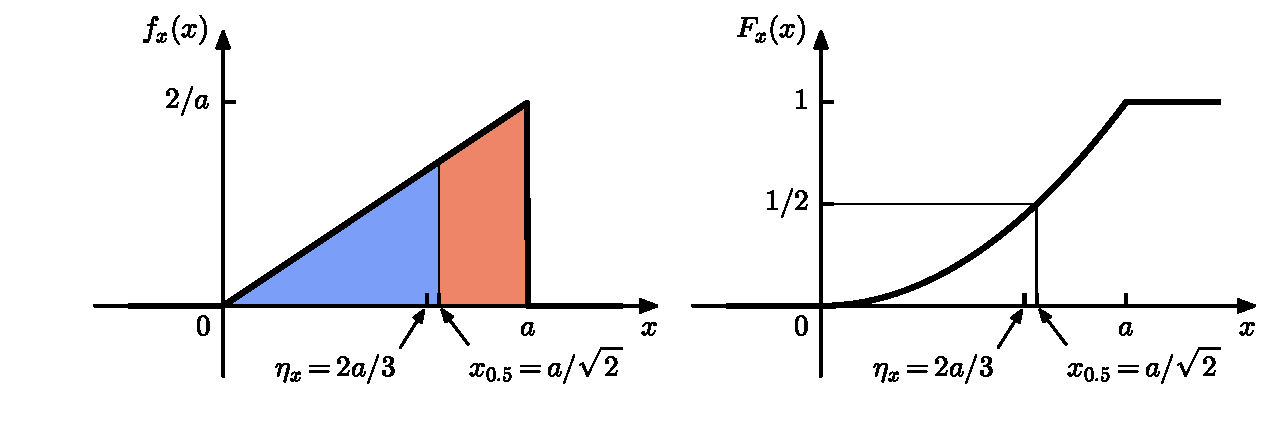
\includegraphics[width=\textwidth]{figuras/mean_and_median_example.pdf}
  \caption{
       Funciones densidad y distribución de probabilidad de la variable aleatoria \(\x\). Por ser una densidad no simétrica, la media y la mediana no coinciden. La mediana es el valor de \(x\) que divide a la densidad de probabilidad en áreas iguales de valor 1/2. Asimismo, la mediana es el valor de \(x\) donde la distribución de probabilidad vale 1/2.
    } \label{fig:mean_and_median_example}
\end{center}
\end{figure}

Se calculará a continuación la mediana \(m\) de la variable aleatoria \(\x\), que por definición es \(F_x(m)=1/2\), o equivalentemente, el percentil 0.5 de \(\x\), \(m=x_{0.5}\). Para hacerlo, se comienza calculando la distribución de probabilidad \(F_x(x)\),
\[
 F_x(x)=\int_{-\infty}^xf_x(u)\,du
   =\frac{2}{a^2}\int_0^xu\,du
   =\frac{2}{a^2}\left(\frac{u^2}{2}\bigg|_0^x\right)
   =\frac{x^2}{a^2},\qquad 0\leq x\leq a,
\]
es decir,
\[\def\arraystretch{1.5}
F_x(x)=\left\{
 \begin{array}{ll}
 0,&x<0\\
 \left(\dfrac{x}{a}\right)^2,&0\leq x\leq a\\
 1,&x>a
 \end{array}\right.,
\]
como se muestra en la figura \ref{fig:mean_and_median_example}. La mediana de \(\x\) es \(x_{0.5}\) tal que
\[
 F_x(x_{0.5})=\left(\dfrac{x_{0.5}}{a}\right)^2=\frac{1}{2},
\]
por lo que despejando se obtiene que \(x_{0.5}=a/\sqrt{2}\). Se concluye que la media y la mediana de la variable aleatoria \(\x\) son respectivamente
\[
 \eta_x=\frac{2a}{3},\qquad x_{0.5}=\frac{a}{\sqrt{2}}.
\]
Notar que por definición, la mediana es el valor de \(x\) que divide la densidad de probabilidad en áreas iguales, como se muestra en la figura \ref{fig:mean_and_median_example}, o equivalentemente, el valor de \(x\) tal que la distribución de probabilidad valga 1/2. Efectivamente, el área a la izquierda de la mediana en la densidad de probabilidad es
\[
 \frac{1}{2}x_{0.5}f_x(x_{0.5})=\frac{1}{2}x_{0.5}\left(\frac{2}{a^2}x_{0.5}\right)=\left(\dfrac{x_{0.5}}{a}\right)^2=\frac{1}{2},
\]
donde se consideró que la superficie es triangular. Como el área bajo la densidad de probabilidad es uno, el área a la derecha de la mediana también es 1/2. 

Observar que en general, la media es distinta a la mediana. La situación particular en que son iguales es cuando la variable aleatoria \(\x\) tiene densidad de probabilidad simétrica respecto a algún valor de \(x\), en cuyo caso, la media y la mediana son ese valor de simetría.

\section{Momentos}

\subsection{Definiciones}

\bgroup
\def\arraystretch{2.5}
\begin{tabular}{lc} 
\textbf{Momentos:} & \(\displaystyle m_n=E\{\x^n\}=\int_{-\infty}^{\infty}x^nf(x)dx\)\\ 
\textbf{Momentos centrales:} & \(\displaystyle \mu_n=E\{(\x-\eta)^n\}=\int_{-\infty}^{\infty}(x-\eta)^nf(x)dx\)\\
\textbf{Momentos absolutos:} & \(\displaystyle E\{|\x|^n\},\qquad E\{|\x-\eta|^n\}\)\\
\textbf{Momentos generalizados:} & \(\displaystyle E\{(\x-a)^n\},\qquad E\{|\x-a|^n\}\)
\end{tabular}
\egroup

\paragraph{Consideraciones} Los momentos de menor orden son

\bgroup
\def\arraystretch{2.5}
\begin{center}
\begin{tabular}{c|c} 
\textbf{Momentos} & \textbf{Momentos centrales}\\ 
\(m_0=E\{\x^0\}=E\{1\}=1\)    & \(\mu_0=E\{(\x-\eta)^0\}=E\{1\}=1\)\\
\(m_1=E\{\x\}\triangleq\eta\) & \(\mu_1=E\{(\x-\eta)\}=E\{\x\}-\eta=0\)\\
                              & \(\mu_2=E\{(\x-\eta)^2\}\triangleq\sigma^2\)
\end{tabular}
\end{center}
\egroup

Los momentos centrales pueden expresarse en función de los momentos, ya que
\begin{align*}
 \mu_n&=E\{(\x-\eta)^n\}\\
   &\overset{(a)}{=}E\left\{\sum_{k=0}^{n}\binom{n}{k}\x^k\left(-\eta\right)^{n-k}\right\}\\
   &\overset{(b)}{=}\sum_{k=0}^{n}\binom{n}{k}E\left\{\x^k\right\}\left(-\eta\right)^{n-k},
\end{align*}
donde en \((a)\) se empleó el teorema del binomio, dado por la ecuación \ref{eq:binomial_theorem}, y en \((b)\) la propiedad de linealidad de la esperanza. Esto resulta en
\begin{equation}\label{eq:central_moments_as_function_of_moments}
 \mu_n=\sum_{k=0}^{n}\binom{n}{k}m_k\left(-\eta\right)^{n-k}.
\end{equation}

Análogamente, los momentos pueden expresarse en función de los momentos centrales,
\begin{align*}
 m_n&=E\{\x^n\}\\
      &=E\{\left[(\x-\eta)+\eta\right]^n\}\\
      &=E\left\{\sum_{k=0}^{n}\binom{n}{k}(\x-\eta)^k\eta^{n-k}\right\}\\
      &=\sum_{k=0}^{n}\binom{n}{k}E\left\{(\x-\eta)^k\right\}\eta^{n-k},
\end{align*}
resultando en
\begin{equation}\label{eq:moments_as_function_of_central_moments}
 m_n=\sum_{k=0}^{n}\binom{n}{k}\mu_k\eta^{n-k}.
\end{equation}
Por ejemplo, el momento cuarto \(m_4=E\{\x^4\}\) en función de los momentos centrales es
\[\arraycolsep=1.4pt\def\arraystretch{2.2}
\begin{array}{*{11}{>{\displaystyle}c}}
  m_4&=&\binom{4}{0}\mu_0\eta^4&+&\binom{4}{1}\mu_1\eta^3&+&\binom{4}{2}\mu_2\eta^2&+&\binom{4}{3}\mu_3\eta&+&\binom{4}{4}\mu_4\\
     &=&1\cdot1\cdot\eta^4&+&4\cdot0\cdot\eta^3&+&6\sigma^2\eta^2&+&4\mu_3\eta&+&\mu_4,\\
     &=&\eta^4&&&+&6\sigma^2\eta^2&+&4\mu_3\eta&+&\mu_4.
\end{array}
\]
A modo de resumen, se cumple que los primeros momentos en función de los momentos centrales son 
\begin{equation}\label{eq:moments_as_function_of_central_moments_first_4}
 \begin{aligned}
 m_2&=\eta^2+\sigma^2\\
 m_3&=\eta^3+3\sigma^2\eta+\mu_3\\
 m_4&=\eta^4+6\sigma^2\eta^2+4\mu_3\eta+\mu_4,
 \end{aligned}
\end{equation}
los cuales se deducen de la ecuación \ref{eq:moments_as_function_of_central_moments}. Notar que la primera ecuación es la misma que la ecuación \ref{eq:variance_definition2}.

\subsection{\texorpdfstring{Momentos de \(\y=\x+b\)}{}}\label{sec:density_shift_moments}

\paragraph{Media} En la sección \ref{sec:y_equals_ax_plus_b_distribution} se calculó la densidad de probabilidad de \(\y=a\x+b\) obteniendo la ecuación \ref{eq:y_equals_ax_plus_b_density}. En el caso en que \(a=1\) en la ecuación \ref{eq:y_equals_ax_plus_b_density}, se tiene que
\[
 \y=\x+b\qquad\Rightarrow\qquad f_y(y)=f_x(x-b),
\]
es decir, la densidad de probabilidad de \(\y\) es la densidad de probabilidad de \(\x\) desplazada horizontalmente una cantidad \(b\). Si \(b>0\), el desplazamiento es hacia la derecha. Evidentemente, la media de \(\y\) va a estar desplazada la misma cantidad. Si la media de \(\x\) es \(\eta_x\), entonces la media \(\eta_y\) de \(\y\) es
\[
 \eta_y=E\{\y\}=E\{\x+b\}=E\{\x\}+b=\eta_x+b.
\]

\paragraph{Momentos centrales} Los momentos centrales de las variables aleatorias \(\x\) e \(\y=\x+b\) son iguales. Efectivamente, los momentos centrales \(\mu_n(y)\) de \(\y\) son
\begin{align*}
 \mu_n(y)&\triangleq\int_{-\infty}^{\infty}(y-\eta_y)^nf_y(y)\,dy\\ 
    &\overset{(a)}{=}\int_{-\infty}^{\infty}\left[y-(\eta_x+b)\right]^nf_x(y-b)\,dy\\
    &\overset{(b)}{=}\int_{-\infty}^{\infty}(x-\eta_x)^nf_x(x)\,dx\\
    &=\mu_n(x),
\end{align*}
donde en \((a)\) se usó que \(f_y(y)=f_x(y-b)\) y \(\eta_y=\eta_x+b\) como se mencionó arriba, y en \((b)\) se realizó el cambio de variable \(x=y-b\).

\subsection{Momentos de una variable aleatoria normal}\label{sec:normal_rv_moments}

Se demostrará a continuación que si
\[
 f(x)=\frac{1}{\sigma\sqrt{2\pi}}e^{-x^2/2\sigma^2}
\]
entonces
\begin{equation}\label{eq:gaussian_rv_moments}
 E\{\x^n\}=
 \left\{\begin{array}{ll}
  1\cdot 3\dots(n-1)\sigma^n, & \textrm{si }n=2k \\
  0, & \textrm{si }n=2k+1
 \end{array} \right.
\end{equation}
\begin{equation}\label{eq:gaussian_rv_absolute_moments}
 E\{|\x|^n\}=
 \left\{\begin{array}{ll}
  1\cdot 3\dots(n-1)\sigma^n, & \textrm{si }n=2k \\
  2^kk!\sigma^{2k+1}\sqrt{2/\pi}, & \textrm{si }n=2k+1.
 \end{array} \right.
\end{equation}

Se comenzará demostrando la ecuación \ref{eq:gaussian_rv_moments}. Los momentos impares son nulos debido a que si \(n\) es impar, la función \(x^nf(x)\) es impar por ser el producto de una función impar con una función par, por lo que su integral es nula. Esto se cumple para cualquier variable aleatoria de densidad de probabilidad par. Para demostrar el resultado con \(n\) par, se considera la siguiente identidad,
\begin{equation}\label{eq:gaussian_integral_with_alpha}
 \int_{-\infty}^{\infty}e^{-\alpha x^2}\,dx=\sqrt{\frac{\pi}{\alpha}},
\end{equation}
que se verifica notando que se trata de una integral gaussiana de la forma de la ecuación \ref{eq:random_gaussian_integral_with_sigma} con \(2\sigma^2=1/\alpha\). Se diferenciará la ecuación \ref{eq:gaussian_integral_with_alpha} respecto a \(\alpha\) \(k\) veces. La derivada del integrando es
\[\arraycolsep=1.4pt\def\arraystretch{2.2}
 \begin{array}{lll}
  \dfrac{\partial}{\partial \alpha}\left(e^{-\alpha x^2}\right)&=&-x^2e^{-\alpha x^2}\\
  \dfrac{\partial^2}{\partial \alpha^2}\left(e^{-\alpha x^2}\right)&=&x^4e^{-\alpha x^2}\\
  \dfrac{\partial^3}{\partial \alpha^3}\left(e^{-\alpha x^2}\right)&=&-x^6e^{-\alpha x^2}
 \end{array}
 \qquad
 \Rightarrow
 \qquad
 \dfrac{\partial^k}{\partial \alpha^k}\left(e^{-\alpha x^2}\right)=(-1)^kx^{2k}e^{-\alpha x^2}
\]
El lado derecho de la ecuación \ref{eq:gaussian_integral_with_alpha}, es una constante multiplicada por \(\alpha^{-1/2}\). Derivando sucesivamente \(\alpha^{-1/2}\) se ve que
\[\arraycolsep=1.4pt\def\arraystretch{2.2}
 \begin{array}{lllll}
  \dfrac{\partial}{\partial \alpha}\left(\alpha^{-1/2}\right)&
     =&-\dfrac{1}{2}\alpha^{-3/2}&=&-\dfrac{1}{2}\cdot\dfrac{1}{\sqrt{\alpha^3}}\\
  \dfrac{\partial^2}{\partial \alpha^2}\left(\alpha^{-1/2}\right)&
     =&\dfrac{1\cdot 3}{2^2}\alpha^{-5/2}&=&\dfrac{1\cdot 3}{2^2}\cdot\dfrac{1}{\sqrt{\alpha^5}}\\
  \dfrac{\partial^3}{\partial \alpha^3}\left(\alpha^{-1/2}\right)&
     =&-\dfrac{1\cdot 3\cdot 5}{2^3}\alpha^{-7/2}&=&-\dfrac{1\cdot 3\cdot 5}{2^3}\cdot\dfrac{1}{\sqrt{\alpha^7}}
 \end{array}
\]
y luego de derivar \(k\) veces, se obtiene que
\[
 \frac{\partial^k}{\partial \alpha^k}\left(\alpha^{-1/2}\right)=(-1)^k\dfrac{1\cdot 3\cdot 5\cdots(2k-1)}{2^k}\cdot\dfrac{1}{\sqrt{\alpha^{2k+1}}}.
\]
A partir de estos resultados, se obtiene que la derivada \(k\)-ésima de la ecuación \ref{eq:gaussian_integral_with_alpha} es
\[
 \int_{-\infty}^{\infty}x^{2k}e^{-\alpha x^2}\,dx=\dfrac{1\cdot 3\cdot 5\cdots(2k-1)}{2^k}\sqrt{\dfrac{\pi}{\alpha^{2k+1}}}.
\]
Sustituyendo \(\alpha=1/2\sigma^2\), se obtiene que
\[
 \int_{-\infty}^{\infty}x^{2k}e^{-x^2/2\sigma^2}\,dx=\dfrac{1\cdot 3\cdot 5\cdots(2k-1)}{2^k}\sqrt{2^{2k+1}\sigma^{2(2k+1)}\pi}.
\]
Operando el término de la raíz cuadrada, se ve que
\[
 \sqrt{2^{2k+1}\sigma^{2(2k+1)}\pi}=\sqrt{2\cdot2^{2k}\sigma^{2}\sigma^{4k}\pi}
 =\sqrt{2\pi\sigma^{2}}\sqrt{2^{2k}\sigma^{4k}}=\sqrt{2\pi\sigma^{2}}2^{k}\sigma^{2k},
\]
y por lo tanto
\[
 \frac{1}{\sqrt{2\pi\sigma^{2}}}\int_{-\infty}^{\infty}x^{2k}e^{-x^2/2\sigma^2}\,dx =1\cdot 3\cdot 5\cdots(2k-1)\sigma^{2k},
\]
y con \(n=2k\) se obtiene la ecuación \ref{eq:gaussian_rv_moments}.

Para demostrar la ecuación \ref{eq:gaussian_rv_absolute_moments}, se observa que \(E\{|\x|^{2k}\}=E\{\x^{2k}\}\), y por lo tanto coincide con el resultado de la ecuación \ref{eq:gaussian_rv_moments} si \(n\) es par. Si \(n=2k+1\) impar, se ve que
\begin{align*}
 E\{|\x|^{2k+1}\}&\overset{(a)}{=}\frac{2}{\sqrt{2\pi\sigma^{2}}}\int_{0}^{\infty}x^{2k+1}e^{-x^2/2\sigma^2}\,dx\\
   &=\frac{1}{\sigma}\sqrt{\frac{2}{\pi}}\int_{0}^{\infty}(x^{2})^{k}e^{-x^2/2\sigma^2}\,xdx\\
   &\overset{(b)}{=}\frac{1}{\sigma}\sqrt{\frac{2}{\pi}}
   \int_{0}^{\infty}\left(2\sigma^2y\right)^ke^{-y}\,\sigma^2dy\\
   &=2^k\sigma^{2k+1}\sqrt{\frac{2}{\pi}}\int_{0}^{\infty}y^ke^{-y}\,dy\\
   &\overset{(c)}{=}2^k\sigma^{2k+1}\sqrt{\frac{2}{\pi}}\Gamma(k+1)\\
   &\overset{(d)}{=}2^k\sigma^{2k+1}\sqrt{\frac{2}{\pi}}k!,
\end{align*}
donde en \((a)\) se usó el hecho de que \(|x|^{2k+1}f(x)\) es una función par, por lo que la integral entre \(-\infty\) a \(\infty\) es el doble que la integral entre 0 a \(\infty\), en \((b)\) se realizó el cambio de variable \(y=x^2/2\sigma^2\) por lo que \(xdx=\sigma^2dy\), en \((c)\) se notó que la integral es la función gamma definida en la ecuación \ref{eq:gamma_function} evaluada en \(k+1\) y en \((d)\) se usó el resultado de la ecuación \ref{eq:gamma_function_equals_factorial} que indica que \(\Gamma(k+1)=k!\).

Notar además que como en este caso la variable aleatoria es de media nula, los momentos y los momentos centrales coinciden. Por lo tanto, los momentos centrales de \(\x\sim N(0,\,\sigma^2)\) están dados por la ecuación \ref{eq:gaussian_rv_moments}. 

A modo ilustrativo, se calculará el momento cuarto de una variable aleatoria \(\x\sim N(0,\,\sigma^2)\) resolviendo la integral de forma similar a la realizada en la sección \ref{sec:normal_mean_and_variance}. Para hacerlo, se puede aplicar la técnica de integración por partes como sigue,
\begin{align*}
 E\{\x^4\}&=\frac{1}{\sqrt{2\pi\sigma^2}}\int_{-\infty}^{\infty} x^4e^{-x^2/2\sigma^2}\,dx\\
 &\overset{(a)}{=}\frac{1}{\sqrt{2\pi\sigma^2}}\left(-\sigma^2x^3e^{-x^2/2\sigma^2}\bigg|_{-\infty}^{\infty} +3\sigma^2\int_{-\infty}^{\infty}e^{-x^2/2\sigma^2}\,dx\right)\\
 &=3\sigma^2\left(\frac{1}{\sqrt{2\pi\sigma^2}}\int_{-\infty}^{\infty}e^{-x^2/2\sigma^2}\,dx\right)\\
 &\overset{(b)}{=}3\sigma^4,
\end{align*}
donde en \((a)\) se aplicó integración por partes, \(\int udv=uv-\int vdu\), con \(u=x^3\) y \(dv=xe^{-x^2/2\sigma^2}dx\) por lo que \(du=3x^2dx\) y \(v=-\sigma^2e^{-x^2/2\sigma^2}\), y en \((b)\) se observó que el factor entre paréntesis es \(\sigma^2\), como se calculó en la sección \ref{sec:normal_mean_and_variance}.


\paragraph{Caso con media no nula} 

Se calcularán a continuación los momentos de una variable aleatoria \(\x\sim N(\eta,\,\sigma^2)\). Debido al argumento dado en la sección \ref{sec:density_shift_moments}, los momentos centrales son iguales a los de la variable aleatoria \(\x'\sim N(0,\,\sigma^2)\), ya que \(\x=\x'+\eta\), y por lo tanto, están dados por la ecuación \ref{eq:gaussian_rv_moments}. Los primeros momentos centrales son
\begin{align*}
 \mu_2=\sigma^2,\qquad\mu_4=3\sigma^4,\qquad\mu_6=15\sigma^6
\end{align*}

Los momentos \(m_n=E\{\x^n\}\) pueden calcularse a partir de los momentos centrales empleando la ecuación \ref{eq:moments_as_function_of_central_moments}. En la ecuación \ref{eq:moments_as_function_of_central_moments_first_4} se indican los cuatro primeros momentos, y sustituyendo los momentos centrales, se obtiene que
\begin{equation}\label{eq:normal_rv_moments}
 \begin{aligned}
 m_2&=\eta^2+\sigma^2\\
 m_3&=\eta(\eta^2+3\sigma^2)\\
 m_4&=\eta^4+6\sigma^2\eta^2+3\sigma^4.
\end{aligned}
\end{equation}

\subsection{Desigualdad de Chebyshev}

Una medida de la concentración de una variable aleatoria en torno a su media \(\eta\) es su varianza \(\sigma^2\). El siguiente teorema muestra que la probabilidad de que la variable aleatoria \(\x\) tome un valor fuera del intervalo \((\eta-\epsilon,\,\eta+\epsilon)\) es despreciable si la razón \(\sigma/\epsilon\) es suficientemente pequeña.

\paragraph{Teorema: desigualdad de Chebyshev} Para cualquier \(\epsilon>0\), se cumple que
\begin{equation}\label{eq:chebyshev_inequality}
 P\{|\x-\eta|\geq\epsilon\}\leq \frac{\sigma^2}{\epsilon^2}
\end{equation}

\paragraph{Demostración} Se parte notando que
\[
 \{|\x-\eta|\geq\epsilon\} \quad \Leftrightarrow \quad \{\x-\eta\geq\epsilon\}\cup\{-\x+\eta\geq\epsilon\} 
 \quad \Leftrightarrow \quad \{\x\geq\eta+\epsilon\}\cup\{\x\leq\eta-\epsilon\},
\]
y por lo tanto
\[
 P\{|\x-\eta|\geq\epsilon\}=\int_{-\infty}^{\eta-\epsilon}f(x)\,dx+\int_{\eta+\epsilon}^{\infty}f(x)\,dx=\int_{|\x-\eta|\geq\epsilon}f(x)\,dx.
\]
Por otro lado, se tiene que
\begin{align*}
 \sigma^2&=\int_{-\infty}^{\infty}(x-\eta)^2f(x)\,dx\\
   &\overset{(a)}{\geq}\int_{|\x-\eta|\geq\epsilon}(x-\eta)^2f(x)\,dx\\
   &\overset{(b)}{\geq}\epsilon^2\int_{|\x-\eta|\geq\epsilon}f(x)\,dx\\
   &\overset{(c)}{=}\epsilon^2P\{|\x-\eta|\geq\epsilon\},
\end{align*}
donde la desigualdad en \((a)\) proviene de que el integrando es positivo y se redujo el intervalo de integración, en \((b)\) se notó que \((x-\eta)^2\geq\epsilon^2\) para todo \(x\) del intervalo de integración y en \((c)\) que la integral es \(P\{|\x-\eta|\geq\epsilon\}\).

La importancia de la desigualdad de Chebyshev es que es válida para variables aleatorias de cualquier distribución, y por lo tanto puede ser usada incluso con variables aleatorias de distribución desconocida. Sin embargo, la cota establecida por la desigualdad, es en general demasiado alta.

\subsection{Desigualdad de Markov}

\paragraph{Teorema: desigualdad de Markov} Si la variable aleatoria \(\x\) toma solo valores no-negativos, es decir, \(f(x)=0\) si \(x<0\), se cumple para todo \(\alpha>0\) que
\begin{equation}\label{eq:markov_inequality}
 P\{\x\geq\alpha\}\leq\frac{\eta}{\alpha}.
\end{equation}

\paragraph{Demostración} Partiendo de la definición de la media \(\eta=E\{\x\}\) de una variable aleatoria \(\x\), se tiene que
\begin{align*}
 E\{\x\}&\overset{(a)}{=}\int_{0}^{\infty}xf(x)\,dx\\
  &\overset{(b)}{\geq}\int_{\alpha}^{\infty}xf(x)\,dx\\
  &\overset{(c)}{=}\alpha\int_{\alpha}^{\infty}f(x)\,dx,
\end{align*}
donde en \((a)\) se empleó el hecho de que la variable aleatoria es no-negativa, la desigualdad en \((b)\) proviene de que el integrando es no-negativo y se redujo el intervalo de integración y en \((c)\) se observó que \(x\geq\alpha\) para todo \(x\) en e intervalo de integración.

La desigualdad de Chebyshev, dada por la ecuación \ref{eq:chebyshev_inequality} es un caso particular de la desigualdad de Markov. Efectivamente, considerando la variable aleatoria no-negativa \(|\x-\eta|^2\) y \(\alpha=\epsilon^2\) en la desigualdad de Markov, se tiene que
\[
 P\{|\x-\eta|^2\geq\epsilon^2\}\leq\frac{E\left\{|\x-\eta|^2\right\}}{\epsilon^2}=\frac{\sigma^2}{\epsilon^2},
\]
y considerando que 
\[
 P\{|\x-\eta|^2\geq\epsilon^2\}=P\{|\x-\eta|\geq\epsilon\},
\]
se obtiene la ecuación de Chebyshev.

\section{Funciones características}

La \emph{función característica} de una variable aleatoria \(\x\) con densidad de probabilidad \(f(x)\) se define como
\begin{equation}\label{eq:characteristic_function}
 \Phi_x(\omega)=\int_{-\infty}^{\infty}f(x)e^{j\omega x}\,dx.
\end{equation}
Como \(f(x)>0\), esta función es máxima en el origen,
\begin{equation}\label{eq:characteristic_function_maximum}
 |\Phi_x(\omega)|\leq\Phi_x(0)=1,
\end{equation}
ya que
\[
 |\Phi_x(\omega)|=\left|\int_{-\infty}^{\infty}f(x)e^{j\omega x}\,dx\right|
   \leq\int_{-\infty}^{\infty}\left|f(x)e^{j\omega x}\right|\,dx
   =\int_{-\infty}^{\infty}f(x)\,dx
   =\Phi_x(0)=1,
\]
donde se empleó la desigualdad triangular y el hecho de que un densidad de probabilidad intergra a 1.

Si se sustituye \(j\omega\) por \(s\) se obtiene la \emph{función generadora de momentos},
\begin{equation}\label{eq:moment_generating_function}
 \Phibf(s)=\int_{-\infty}^{\infty}f(x)e^{s x}\,dx.
\end{equation}

La función
\[
 \Psi(\omega)=\ln\Phi_x(\omega)=\Psibf(j\omega)
\]
es la \emph{segunda función característica} de \(\x\).

Notar que se cumple que
\[
 \Phi(\omega)=E\{e^{j\omega\x}\},\qquad \Phibf(s)=E\{e^{s\x}\}.
\]
Esto conduce al hecho de que si
\begin{equation}\label{eq:characteristic_function_of_linear_function_of_rv}
 \y=a\x+b\qquad\Rightarrow\qquad \Phi_y(\omega)=e^{jb\omega}\Phi_x(a\omega)
\end{equation}
ya que
\[
 \Phi_y(\omega)=E\{e^{j\omega\y}\}=E\{e^{j\omega(a\x+b)}\}=e^{jb\omega}E\{e^{ja\omega \x}\}=e^{j b\omega}\Phi_x(a\omega).
\]
Análogamente, puede verse que la función generadora de momentos cumple que
\begin{equation}\label{eq:moment_function_of_linear_function_of_rv}
  \Phibf_y(s)=e^{bs}\Phibf_x(as).
\end{equation}

\subsection{Función característica de una variable aleatoria normal}

Se demostrará que la función característica de \(\x\sim N(\eta,\,\sigma^2)\) es
\begin{equation}\label{eq:normal_rv_characteristic_function}
 \Phi_x(\omega)=e^{j\eta\omega-\frac{1}{2}\sigma^2\omega^2}.
\end{equation}
Para ver esto, se considera la variable aleatoria normalizada \(\z=(\x-\eta)/\sigma\). De esta forma, \(\z\sim N(0,\,1)\), y su función generadora de momentos es
\[
 \Phibf_z(s)=\frac{1}{\sqrt{2\pi}}\int_{-\infty}^{\infty}e^{sz}e^{-z^2/2}\,dz.
\]
Observando que el exponente de la exponencial se puede escribir como
\[
 sz-\frac{z^2}{2}=-\frac{1}{2}(z-s)^2+\frac{s^2}{2},
\]
se concluye que
\[
 \Phibf_z(s)=e^{s^2/2}\int_{-\infty}^{\infty}\frac{1}{\sqrt{2\pi}}e^{-(z-s)^2/2}\,dz=e^{s^2/2},
\]
donde en la segunda igualdad se notó que el integrando es una densidad de probabilidad \(N(s,\,1)\) y por lo tanto tiene área 1. Ahora, como \(\x=\sigma\z+\eta\), usando la ecuación \ref{eq:moment_function_of_linear_function_of_rv} se llega a que
\begin{equation}\label{eq:normal_rv_moment_function}
 \Phibf_x(s)=e^{\eta s}e^{\sigma^2s^2/2}=e^{\eta s+\frac{1}{2}\sigma^2s^2},
\end{equation}
y sustituyendo \(s\) por \(j\omega\) se obtiene la función característica dada por la ecuación \ref{eq:normal_rv_characteristic_function}. Además, la segunda función característica de \(\x\) es
\begin{equation}\label{eq:normal_rv_second_characteristic_function}
 \Psi_x(\omega)=\ln\Phi_x(\omega)=j\eta\omega-\frac{1}{2}\sigma^2\omega^2.
\end{equation}

\paragraph{Fórmula de inversión}

De la definición de la función característica dada por la ecuación \ref{eq:characteristic_function}, se observa que \(\Phi_x(\omega)\) es la transformada de Fourier de \(f(x)\). Por lo tanto, \(f(x)\) puede expresarse en términos de \(\Phi_x(\omega)\) a partir de la transformada inversa,
\begin{equation}\label{eq:characteristic_function_inversion}
 f(x)=\frac{1}{2\pi}\int_{-\infty}^{\infty}\Phi_x(\omega)e^{-j\omega x}\,d\omega.
\end{equation}

\paragraph{Inversión de la función característica de una variable aleatoria normal}

Como ejemplo, se invertirá la función característica de una variable aleatoria normal. Aplicando la fórmula de inversión, dada por la ecuación \ref{eq:characteristic_function_inversion}, a la ecuación \ref{eq:normal_rv_characteristic_function}, se tiene que
\begin{equation}\label{eq:normal_characteristic_function_inversion}
  f(x)=\frac{1}{2\pi}\int_{-\infty}^{\infty}e^{j\eta\omega-\frac{1}{2}\sigma^2\omega^2}e^{-j\omega x}\,d\omega
 =\frac{1}{2\pi}\int_{-\infty}^{\infty}e^{-\frac{1}{2}\sigma^2\omega^2-j\omega(x-\eta)}\,d\omega.
\end{equation}
Se expresará el exponente de la exponencial del integrando usando la técnica de ``completar el cuadrado''\footnote{ver \url{https://en.wikipedia.org/wiki/Completing_the_square}}, que consiste en observar que un polinomio de segundo grado puede expresarse como
\begin{equation}\label{eq:complete_squares_one_variable}
 \frac{1}{2}az^2+bz+c=\frac{1}{2}a\left(z+\frac{b}{a}\right)^2+c-\frac{b^2}{2a}.
\end{equation}
Tomando
\[
 z=\omega,\qquad a=\sigma^2,\qquad b=j(x-\eta),\qquad c=0,
\]
el exponente del integrando puede escribirse como
\[
 -\frac{1}{2}\sigma^2\omega^2-j\omega(x-\eta)=-\frac{1}{2}\sigma^2\left[\omega+\frac{j(x-\eta)}{\sigma^2}\right]^2-\frac{(x-\eta)^2}{2\sigma^2}.
\]
De esta forma,
\begin{equation}\label{eq:gaussian_integral_complex_offset_tmp1}
 f(x)=\frac{1}{2\pi}\exp\left[-\frac{(x-\eta)^2}{2\sigma^2}\right]\int_{-\infty}^{\infty}\exp\left\{-\frac{1}{2}\sigma^2\left[\omega+\frac{j(x-\eta)}{\sigma^2}\right]^2\right\}\,d\omega.
\end{equation}
Notar que el beneficio de expresar el exponente de esta forma es que un término del producto de exponenciales no depende de la variable de integración y por lo tanto puede sacarse de la integral, y el otro término es una exponencial con exponente al cuadrado. Se obtiene entonces una integral gaussiana similar a la de la ecuación \ref{eq:gaussian_integral_with_alpha}, excepto que en este caso, la variable de integración está afectada por el desplazamiento complejo \(j(x-\eta)/\sigma^2\). Para resolver la integral, se demostrará que \cite{smith2011spectral_chap_gaussian}
%%%%%%%%%%%%%%%%%%%%%%%%%%%%%%%%%%%%%%%%%%%%%%%%%%%%%%%%%%%%%%%%%%%%%%%%%%%%%%%%%%%%%%%%%
%%%%%%%%%%%%%%%%%%%%%%%%%%%%%%%%%%%%%%%%%%%%%%%%%%%%%%%%%%%%%%%%%%%%%%%%%%%%%%%%%%%%%%%%%
% Sacado del documento "Técnicas clásicas de representación tiempo-frecuencia" de
% López-Rocamora, 2010.
\[
 \int_{-\infty}^{\infty}e^{-p(t+c)^2}\,dt = \int_{-\infty}^{\infty}e^{-pt^2}\,dt,\quad\textrm{con}\quad p,c\in\mathbb{C},\; \textrm{Re}\{p\}>0.
\]
Considérese la curva rectangular \(\Gamma_c(T)\) que se ilustra en la figura \ref{fig:gaussian_integral_complex_offset}, y está formada por las rectas  
\[
\begin{array}{lc}
\Gamma_{c_1}(T) : z=x,& -T<x<T \\
\Gamma_{c_2}(T) : z=T+iy,& 0<y<b \\ 
\Gamma_{c_3}(T) : z=x+ib,& -T<x<T \\
\Gamma_{c_4}(T) : z=-T+iy,& 0<y<b.
\end{array}
\]
La función \(f(z) \triangleq e^{-pz^2}\) es analítica dentro de la región limtada por \(\Gamma_c(T)\) y por lo tanto el teorma integral de Cauchy\footnote{\textbf{Enunciado}: Sea \(D\) un subconjunto abierto de \(\mathbb{C}\), sea \(f:D\rightarrow \mathbb{C}\) una función analítica y sea \(\Gamma\) un contorno cerrado simple contenido en \(D\), entonces \(\oint_\Gamma f(z)\,dz = 0\).} indica que
\begin{equation}\label{eq:gaussian_integral_complex_offset_tmp2}
 \oint_{\Gamma_c} f(z)\,dz = 0.
\end{equation}
\begin{figure}[!htb]
  \begin{minipage}[c]{0.5\textwidth}
    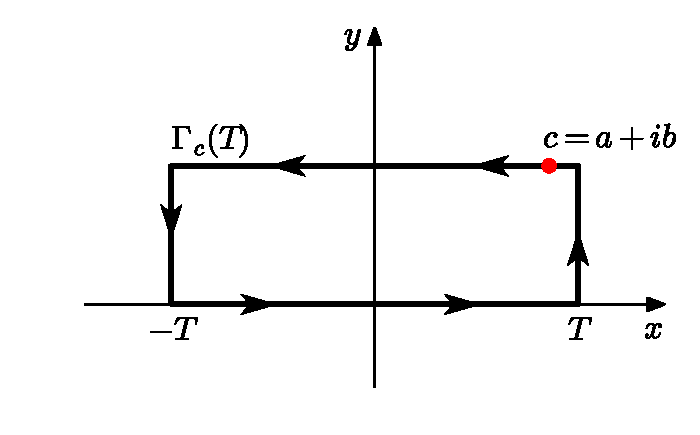
\includegraphics[width=\textwidth]{figuras/gaussian_integral_complex_offset.pdf}
  \end{minipage}\hfill
  \begin{minipage}[c]{0.47\textwidth}
    \caption{
       Camino de integración \(\Gamma_c(T)\) de la ecuación \ref{eq:gaussian_integral_complex_offset_tmp2}. \(\Gamma_c(T)\) es un rectángulo con un lado que coincide con el eje \(x\) y el lado opuesto pasa por el desplazamiento complejo \(c\).
    } \label{fig:gaussian_integral_complex_offset}
  \end{minipage}
\end{figure}
Considerando la integral en cada uno de los caminos rectos se tiene que
\begin{align*}
\oint_{\Gamma_c(T)} f(z)\,dz &= \oint_{\Gamma_{c_1}(T)} f(z)\,dz+\oint_{\Gamma_{c_2}(T)} f(z)\,dz+\oint_{\Gamma_{c_3}(T)} f(z)\,dz \\
 &\qquad+\oint_{\Gamma_{c_4}(T)} f(z)\,dz \\
 &= \int_{-T}^{T}f(x)\,dx + \int_{0}^{b}f(T+iy)i\,dy + \int_{T}^{-T}f(x+ib)\,dx \\
 &\qquad + \int_{b}^{0}f(-T+iy)i\,dy,
\end{align*}
donde \(x,\,y\in\mathbb{R}\). Tomando \(|T|\to \infty\), el integrando del segundo sumando \(e^{-p(T+iy)^2}\to 0\) y lo mismo ocurre con el cuarto sumando. Por lo tanto,
\[
 \int_{-\infty}^{\infty}e^{-p(x+ib)^2}\,dx = \int_{-\infty}^{\infty}e^{-px^2}\,dx.
\]
Haciendo el cambio de variable \(x=t+a=t+c-ib\) en la integral de la izquierda de la igualdad, se concluye que
\[
 \int_{-\infty}^{\infty}e^{-p(t+c)^2}\,dx = \int_{-\infty}^{\infty}e^{-pt^2}\,dt,
\]
que es lo que se quería demostrar.
%%%%%%%%%%%%%%%%%%%%%%%%%%%%%%%%%%%%%%%%%%%%%%%%%%%%%%%%%%%%%%%%%%%%%%%%%%%%%%%%%%%%%%%%%
%%%%%%%%%%%%%%%%%%%%%%%%%%%%%%%%%%%%%%%%%%%%%%%%%%%%%%%%%%%%%%%%%%%%%%%%%%%%%%%%%%%%%%%%%
Este resultado indica que la integral de la ecuación \ref{eq:gaussian_integral_complex_offset_tmp1}  es
\[
 f(x)=\frac{1}{2\pi}\exp\left[-\frac{(x-\eta)^2}{2\sigma^2}\right]\int_{-\infty}^{\infty}e^{-\sigma^2\omega/2}\,d\omega.
\]
Considerando que la integral es gaussiana, usando el resultado de la ecuación \ref{eq:gaussian_integral_with_alpha}, se tiene que
\[
 \int_{-\infty}^{\infty}e^{-\sigma^2\omega/2}\,d\omega =  \sqrt{\frac{2\pi}{\sigma^2}},
\]
por lo que se concluye que
\[
 f(x)=\frac{1}{\sqrt{2\pi\sigma^2}}\exp\left[-\frac{(x-\eta)^2}{2\sigma^2}\right],
\]
que es la densidad de probabilidad de una variable aleatoria normal de media \(\eta\) y varianza \(\sigma^2\).

Se explica a continuación una deducción alternativa de la inversión de la función característica de una variable aleatoria normal\footnote{Esta deducción está basada en:\\Sasha, Characteristic function of a standard normal random variable, URL (version: 2011-12-10): \url{https://math.stackexchange.com/q/86048}.}. Partiendo de la ecuación \ref{eq:normal_characteristic_function_inversion}, se ve que
\begin{align*}
 f(x)&=\frac{1}{2\pi}\int_{-\infty}^{\infty}e^{-\frac{1}{2}\sigma^2\omega^2}e^{-j\omega(x-\eta)}\,d\omega\\
 &=\frac{1}{2\pi}\int_{-\infty}^{0}e^{-\frac{1}{2}\sigma^2\omega^2}e^{-j\omega(x-\eta)}\,d\omega+ 
 \frac{1}{2\pi}\int_{0}^{\infty}e^{-\frac{1}{2}\sigma^2\omega^2}e^{-j\omega(x-\eta)}\,d\omega\\
 &=-\frac{1}{2\pi}\int_{\infty}^{0}e^{-\frac{1}{2}\sigma^2u^2}e^{ju(x-\eta)}\,du+ 
 \frac{1}{2\pi}\int_{0}^{\infty}e^{-\frac{1}{2}\sigma^2\omega^2}e^{-j\omega(x-\eta)}\,d\omega,
\end{align*}
donde en la última igualdad se realizó el cambio de variable \(u=-\omega\) en la primer integral. Intercambiando los límites de integración y cambiando el signo en la primer integral, así como renombrando la variable de integración a \(\omega\), se tiene que
\begin{align*}
 f(x)&=\frac{1}{2\pi}\int_{0}^{\infty}e^{-\frac{1}{2}\sigma^2\omega^2}e^{j\omega(x-\eta)}\,d\omega+ 
 \frac{1}{2\pi}\int_{0}^{\infty}e^{-\frac{1}{2}\sigma^2\omega^2}e^{-j\omega(x-\eta)}\,d\omega\\
  &=\frac{1}{\pi}\int_{0}^{\infty}e^{-\frac{1}{2}\sigma^2\omega^2}\,\frac{e^{j\omega(x-\eta)}+e^{-j\omega(x-\eta)}}{2}\,d\omega
\end{align*}
Considerando la identidad \(\cos x=(e^{jx}+e^{-jx})/2\), se concluye que
\begin{equation}\label{eq:gaussian_integral_complex_offset_tmp3}
 f(x)=\frac{1}{\pi}\int_{0}^{\infty}e^{-\frac{1}{2}\sigma^2\omega^2}\cos\omega(x-\eta)\,d\omega.
\end{equation}
Derivando respecto a \(x\), se tiene que
\[
 f'(x)=-\frac{1}{\pi}\int_{0}^{\infty}\omega e^{-\frac{1}{2}\sigma^2\omega^2}\sen\omega(x-\eta)\,d\omega,
\]
y aplicando integración por partes, \(\int udv=uv-\int vdu\), con \(u=\sen\omega(x-\eta)\) y \(dv=\omega e^{-\frac{1}{2}\sigma^2\omega^2}\) y por lo tanto \(du=(x-\eta)\cos\omega(x-\eta)\) y \(v=-e^{-\frac{1}{2}\sigma^2\omega^2}/\sigma^2\), se tiene que
\begin{align*}
 f'(x)&=-\frac{1}{\pi}\left[-\frac{e^{-\frac{1}{2}\sigma^2\omega^2}}{\sigma^2}\sen\omega(x-\eta)\bigg|_{0}^{\infty} + \int_{0}^{\infty}\frac{e^{-\frac{1}{2}\sigma^2\omega^2}}{\sigma^2}(x-\eta)\cos\omega(x-\eta)\,d\omega\right]\\
  &=-\frac{(x-\eta)}{\sigma^2}\left[\frac{1}{\pi}\int_{0}^{\infty}e^{-\frac{1}{2}\sigma^2\omega^2}\cos\omega(x-\eta)\,d\omega\right],
\end{align*}
donde se consideró que el primer sumando a la derecha de la primer igualdad se anula, ya que la exponencial se anula con \(\omega\to\infty\) y \(\sin0=0\). Por lo tanto, se obtuvo que
\[
 f'(x)=-\frac{(x-\eta)}{\sigma^2}f(x).
\]
Esta ecuación diferencial puede resolverse dividiendo la igualdad entre \(f(x)\) y considerando que
\[
 \frac{f'(x)}{f(x)}=\frac{d}{dx}\ln f(x).
\]
De esta forma, se obtiene que
\[
 \frac{d}{dx}\ln f(x)=-\frac{(x-\eta)}{\sigma^2}
\]
e integrando en ambos lados de la igualdad se llega a que
\[
 \ln f(x)=-\frac{(x-\eta)^2}{2\sigma^2}+C',
\]
donde \(C'\) es una constante a determinar. Despejando \(f(x)\) se obtiene que
\[
 f(x)=C\exp\left[-\frac{(x-\eta)^2}{2\sigma^2}\right].
\]
Para determinar la constante \(C\) se evalúa esta última ecuación y la ecuación \ref{eq:gaussian_integral_complex_offset_tmp3} en \(x=\eta\) y se igualan los resultados. De esta forma
\begin{align*}
 f(\eta)=C&=\frac{1}{\pi}\int_{0}^{\infty}e^{-\frac{1}{2}\sigma^2\omega^2}\,d\omega\\
   &\overset{(a)}{=}\frac{1}{2\pi}\int_{-\infty}^{\infty}e^{-\frac{1}{2}\sigma^2\omega^2}\,d\omega\\
   &\overset{(b)}{=}\frac{1}{2\pi}\sqrt{\frac{2\pi}{\sigma^2}}\\
   &=\frac{1}{\sqrt{2\pi\sigma^2}},
\end{align*}
donde en \((a)\) se consideró que el integrando es una función par y por lo tanto, la integral entre 0 y \(\infty\) es el doble que la integral entre \(-\infty\) y \(\infty\) y en \((b)\) que es una integral gaussiana y por lo tanto se aplica el resultado de la ecuación \ref{eq:gaussian_integral_with_alpha}. De esta forma, se concluye que
\[
 f(x)=\frac{1}{\sqrt{2\pi\sigma^2}}\exp\left[-\frac{(x-\eta)^2}{2\sigma^2}\right].
\]

\paragraph{Teorema de los momentos} Derivando la ecuación \ref{eq:moment_generating_function} \(n\) veces se obtiene que
\[
 \Phibf^{(n)}(s)=E\left\{\x^ne^{s\x}\right\},
\]
y evaluando en \(s=0\) se concluye que
\begin{equation}\label{eq:moments_theorem}
 \Phibf^{(n)}(0)=E\left\{\x^n\right\}=m_n,
\end{equation}
es decir, las derivadas de \(\Phibf^{(n)}(s)\) en el origen son los momentos de la variable aleatoria \(\x\). De aquí el nombre de función generadora de momentos. En particular,
\[
 \Phibf'(0)=m_1=\eta,\qquad\Phibf''(0)=m_2=\eta^2+\sigma^2.
\]

\paragraph{Observación} Expandiendo \(\Phibf(s)\) en una serie de potencias en torno al origen, se tiene que
\[
 \Phibf(s)=\sum_{n=0}^{\infty}\frac{m_n}{n!}s^n.
\]
Esta expresión es válida si todos los momentos son finitos y la serie converge absolutamente en torno al origen. Debido a que \(f(x)\) puede obtenerse a partir de \(\Phibf(s)\), se concluye que en las condiciones indicadas, la densidad de probabilidad de una variable aleatoria queda unívocamente determinada si se conocen todos sus momentos.

\subsection{Momentos de una variable aleatoria normal}

Como se vió previamente, la función generadora de momentos de una variable aleatoria normal está dada por la ecuación \ref{eq:normal_rv_moment_function},
\[
 \Phibf(s)=e^{\eta s+\frac{1}{2}\sigma^2s^2}.
\]
Por lo tanto,
\[\arraycolsep=1.4pt\def\arraystretch{1.5}
 \begin{array}{lll}
 \Phibf'(s)&=&(\eta+\sigma^2s)e^{\eta s+\frac{1}{2}\sigma^2s^2}\\
 \Phibf''(s)&=&\sigma^2e^{\eta s+\frac{1}{2}\sigma^2s^2}+(\eta+\sigma^2s)^2e^{\eta s+\frac{1}{2}\sigma^2s^2}\\
 \Phibf'''(s)&=&3\sigma^2(\eta+\sigma^2s)e^{\eta s+\frac{1}{2}\sigma^2s^2}+(\eta+\sigma^2s)^3e^{\eta s+\frac{1}{2}\sigma^2s^2}
 \end{array}
\]
y evaluando en \(s=0\) se obtiene que
\[\arraycolsep=1.4pt\def\arraystretch{1.5}
 \begin{array}{lllll}
 m_1&=&\Phibf'(0)&=&\eta\\
 m_2&=&\Phibf''(0)&=&\sigma^2+\eta^2\\
 m_3&=&\Phibf'''(0)&=&3\sigma^2\eta+\eta^3
 \end{array}
\]
coincidiendo con los resultados obtenidos previamente en la ecuación \ref{eq:normal_rv_moments}.

\subsection{Momentos de una variable aleatoria gamma}

Se calcularán los momentos de una variable aleatoria gamma, cuya densidad de probabilidad es
\begin{equation}\label{eq:pdf_gamma_b_lambda}
 f_x(x)=\gamma x^{b-1}e^{-\lambda x}U(x),\qquad\gamma=\frac{\lambda^b}{\Gamma(b)},
\end{equation}
donde se redefinieron los parámetros de la densidad dada en la ecuación \ref{eq:pdf_gamma} como \(\alpha=b\) y \(\beta=1/\lambda\). A partir de la ecuación \ref{eq:moment_generating_function} se obtiene que la función generadora de momentos es
\begin{align*}
 \Phibf(s)&=\gamma\int_{0}^{\infty}x^{b-1}e^{-(\lambda-s) x}\,dx\\
    &\overset{(a)}{=}\gamma\int_{0}^{\infty}\frac{u^{b-1}}{(\lambda-s)^{b-1}}\,e^{-u}\,\frac{du}{\lambda-s}\\
    &=\frac{\gamma}{(\lambda-s)^b}\int_{0}^{\infty}u^{b-1}e^{-u}\,du\\
    &\overset{(b)}{=}\frac{\gamma}{(\lambda-s)^b}\,\Gamma(b),
\end{align*}
donde en \((a)\) se realizó el cambio de variable \(u=(c-s)x\), por lo que \(du=(c-s)dx\) y en \((b)\) se notó que la integral es la función gamma, definida en la ecuación \ref{eq:gamma_function}. Finalmente, se obtiene que
\begin{equation}\label{eq:gamma_moment_generating_function}
 \Phibf(s)=\frac{\lambda^b}{(\lambda-s)^b}=\lambda^b(\lambda-s)^{-b}
\end{equation}
y derivando sucesivamente respecto a \(s\), se ve que
\[\arraycolsep=1.4pt\def\arraystretch{1.5}
 \begin{array}{lcl}
 \Phibf'(s)&=&\lambda^bb(\lambda-s)^{-(b+1)}\\
 \Phibf''(s)&=&\lambda^bb(b+1)(\lambda-s)^{-(b+2)}
 \end{array}
\]
Luego de derivar \(n\) veces, se obtiene que
\begin{equation}\label{eq:gamma_moment_generating_function_n_derivative}
 \Phibf^{(n)}(s)=\frac{\lambda^bb(b+1)\cdots(b+n-1)}{(\lambda-s)^{(b+n)}},
\end{equation}
y evaluando en \(s=0\), se concluye que
\[
 \Phibf^{(n)}(0)=\frac{b(b+1)\cdots(b+n-1)}{\lambda^n}=E\{\x^n\}.
\]
Los dos primeros momentos son
\[
 E\{\x\}=\frac{b}{\lambda},\qquad E\{\x^2\}=\frac{b(b+1)}{\lambda^2},\qquad\sigma^2=E\{\x^2\}-E^2\{\x\}=\frac{b}{\lambda^2}
\]

\subsection{Momentos de una variable aleatoria chi-cuadrado}\label{sec:chi_square_moments}

Una variable aleatoria chi-cuadrado con \(m\) grados de libertad, cuya densidad de probabilidad está dada por la ecuación \ref{eq:pdf_chi_square}, es un caso particular de una variable aleatoria gamma con parámetros \(b=m/2\) y \(\lambda=1/2\) en la densidad de probabilidad de la ecuación \ref{eq:pdf_gamma_b_lambda}. De esta forma, sustituyendo \(b=m/2\) y \(\lambda=1/2\) en la función generadora de momentos (ecuación \ref{eq:gamma_moment_generating_function}) se obtiene que
\[
 \Phibf(s)=\dfrac{\left(\dfrac{1}{2}\right)^{m/2}}{\left(\dfrac{1}{2}-s\right)^{m/2}}
 =\dfrac{\left(\dfrac{1}{2}\right)^{m/2}}{\left(\dfrac{1}{2}\right)^{m/2}\left(1-2s\right)^{m/2}}
 =\frac{1}{(1-2s)^{m/2}},
\]
concluyendo que la función generadora de momentos de una variable aleatoria chi-cuadrado con \(m\) grados de libertad es
\begin{equation}\label{eq:chi_square_moment_generating_function}
 \Phibf(s)=\frac{1}{\sqrt{(1-2s)^m}}.
\end{equation}
De la misma forma, sustituyendo \(b=m/2\) y \(\lambda=1/2\) en la derivada \(n\)-ésima de la función generadora de momentos de la variable aleatoria gamma (ecuación \ref{eq:gamma_moment_generating_function_n_derivative}) se obtiene que
\begin{align*}
 \Phibf^{(n)}(s)&=\dfrac{\left(\dfrac{1}{2}\right)^{m/2}\left[\dfrac{m}{2}\left(\dfrac{m}{2}+1\right)\cdots\left(\dfrac{m}{2}+n-1\right)\right]}{\left(\dfrac{1}{2}-s\right)^{m/2+n}}\\
   &\overset{(a)}{=}\dfrac{\left(\dfrac{1}{2}\right)^{m/2+n}\left[m\left(m+2\right)\cdots\left(m+2n-2\right)\right]}{\left(\dfrac{1}{2}\right)^{m/2+n}\left(1-2s\right)^{m/2+n}}\\
   &=\dfrac{m\left(m+2\right)\cdots\left(m+2n-2\right)}{\left(1-2s\right)^{(m+2n)/2}},
\end{align*}
donde en \((a)\) se sacó denominador común 2 en los \(n\) términos en el producto entre paréntesis rectos y se sacó el factor \(1/2^n\) resultante fuera de los paréntesis, y se hizo lo análogo en el denominador.
Se concluye que la derivada \(n\)-ésima de la función generadora de momentos de una variable aleatoria chi-cuadrado con \(m\) grados de libertad es
\[
 \Phibf^{(n)}(s)=\dfrac{m\left(m+2\right)\cdots\left(m+2n-2\right)}{\sqrt{\left(1-2s\right)^{m+2n}}}.
\]
Evaluando en \(s=0\), se llega a que
\[
 \Phibf^{(n)}(0)=m\left(m+2\right)\cdots\left(m+2n-2\right)=E\{\x^n\}.
\]
Por lo tanto, los dos primeros momentos son
\[
 E\{\x\}=m,\qquad E\{\x^2\}=m(m+2),
\]
y el segundo momento central es
\[
 \sigma^2=E\{\x^2\}-E^2\{\x\}=m(m+2)-m^2=2m.
\]

\subsection{Momentos de una variable aleatoria uniforme}\label{sec:uniform_moments}

Sea una variable aleatoria con distribución uniforme en el intervalo \((a,\,b)\), cuya densidad de probabilidad esta dada por
\[
 f(x)=\left\{
 \begin{array}{ll}
  \dfrac{1}{b-a},& a<x<b\\
  0, &\textrm{en otro caso.}
 \end{array}
 \right.
\]
La función generadora de momentos es
\[
 \Phibf(s)=\frac{1}{b-a}\int_a^be^{sx}\,dx=\frac{1}{b-a}\frac{e^{sx}}{s}\bigg|_a^b=\frac{e^{sb}-e^{sa}}{s(b-a)}.
\]
Considérese el caso particular en que \(a=-T/2\) y \(b=T/2\), por lo que la variable aleatoria tiene distribución uniforme en el intervalo \((-T/2,\,T/2)\). En ese caso, la función generadora de momentos queda
\begin{align*}
 \Phibf(s)&=\frac{e^{sT/2}-e^{-sT/2}}{sT}\\
   &\overset{(a)}{=}\frac{2\sinh(sT/2)}{sT},
\end{align*}
donde en \((a)\) se escribió la expresión en términos de la función seno hiperbólico, que junto a la función coseno hiperbólico se definen respectivamente como
\[
 \sinh x=\frac{e^x-e^{-x}}{2}\qquad\qquad\textrm{y}\qquad\qquad\cosh x =\frac{e^x+e^{-x}}{2}.
\]
Para calcular los momentos, resulta útil realizar una expansión de Taylor en torno a \(s=0\) de la función generadora de momentos. La expansión de Taylor de una función \(f(x)\) en torno a \(x=0\) es
\[
 f(x)=f(0)+\frac{f'(0)}{1!}x+\frac{f''(0)}{2!}x^2+\frac{f'''(0)}{3!}x^3+\dots.
\]
De las definiciones de seno y coseno hiperbólico es fácil ver que
\[
 \sinh 0=0,\qquad\cosh0=1,\qquad\frac{d}{dx}\sinh x=\cosh x,\qquad\frac{d}{dx}\cosh x=\sinh x,
\]
por lo que el desarrollo de Taylor de la función seno hiperbólico es
\[
 \sinh x=x+\frac{x^3}{3!}+\frac{x^5}{5!}+\dots=\sum_{k=0}^\infty\frac{x^{2k+1}}{(2k+1)!}.
\]
Aplicando este resultado, el desarrollo de Taylor de la función generadora de momentos es
\[
 \Phibf(s)=\frac{2}{sT}\sum_{k=0}^\infty\frac{\left(\dfrac{sT}{2}\right)^{2k+1}}{(2k+1)!}
   =\sum_{k=0}^\infty\frac{\left(\dfrac{sT}{2}\right)^{2k}}{(2k+1)!},
\]
es decir,
\begin{equation}\label{eq:uniform_moment_generating_function_taylor}
 \Phibf(s)=\sum_{k=0}^\infty\frac{T^{2k}}{2^{2k}(2k+1)!}s^{2k}.
\end{equation}
Como indica la ecuación \ref{eq:moments_theorem}, la derivada \(n\)-ésima evaluada en cero de la función generadora de momentos, es el momento \(n\)-ésimo de la variable aleatoria. 
Al diferenciar \(2n\) veces y evaluar en \(s=0\), el único término que sobrevive es el que corresponde al coeficiente de grado \(2n\), ya que los de grado menor se anulan al diferenciar y los de grado mayor se anulan al evaluar en \(s=0\), resultando en
\[
  \Phibf^{(2n)}(0)=\frac{T^{2n}(2n)!}{2^{2n}(2n+1)!}=\frac{T^{2n}}{2^{2n}(2n+1)},
\]
donde se tuvo en cuenta además que \(d^nx^n/dx^n=n!\). Se concluye que los momentos de una variable aleatoria uniforme en el intervalo \((-T/2,\,T/2)\) son
\[
 m_{2n}=E\{\x^{2n}\}=\frac{T^{2n}}{2^{2n}(2n+1)},
\]
y los momentos impares son nulos debido a que la densidad de probabilidad es una función simétrica.
Por lo tanto, los primeros momentos son
\[
 E\{\x^2\}=\frac{T^2}{2^2\times3}=\frac{T^2}{12},\qquad\qquad E\{\x^4\}=\frac{T^4}{2^3\times5}=\frac{T^4}{80}.
\]



\paragraph{Cumulantes}

Los cumulantes \(\lambda_n\) de una variable aleatoria \(\x\) se definen como las derivadas de la función generadora de momentos segunda,
\[
 \frac{d\Psibf(0)}{ds^n}=\lambda_n,
\]
y se cumple que 
\[
 \lambda_1=\eta,\qquad\lambda_2=\sigma^2.
\]
Para ver esto, se observa que por definición, \(\Phibf=e^{\Psibf}\) y por lo tanto,
\[
 \Phibf'=\Psibf'e^{\Psibf},\qquad \Phibf''=\left[\Psibf''+\left(\Psibf'\right)^2\right]e^{\Psibf}
\]
Evaluando en \(s=0\) y considerando que \(\Psibf(0)=\lambda_0=0\) ya que
\[
 \Psibf(0)=\ln\Phibf(0)=\ln\left[\int_{-\infty}^{\infty}f(x)\,dx\right]=\ln1=0
\]
y teniendo en cuenta que \(\Phibf^{(n)}(0)=E\{\x^n\}=m_n\), se tiene que
\[
 \Phibf'(0)=\Psibf'(0)=m_1=\eta
\]
y
\[
 \Phibf''(0)=\Psibf''(0)+\left[\Psibf'(0)\right]^2
\]
por lo que
\[
 \Psibf''(0)=\Phibf''(0)-\left[\Psibf'(0)\right]^2=m_2-m_1^2=E\{\x^2\}-E^2\{\x\}=\sigma^2.
\]

\paragraph{Caso discreto} En el caso en que \(\x\) es una variable aleatoria discreta con \(p_i=P\{\x=x_i\}\), la \emph{función característica} se define como
\[
 \Phi_x(\omega)=\sum_i p_ie^{j\omega x_i}
\]

La \emph{función generadora de momentos} puede definirse igual que en el caso continuo (ecuación \ref{eq:moment_generating_function}), pero si la variable aleatoria toma solo valores enteros, es mas apropiado definirla mediante la transformada \(z\) como
\begin{equation}\label{eq:moment_generating_function_discrete}
 \Gammabf(z)=E\{z^\x\}=\sum_{n=-\infty}^{\infty}P\{\x=n\}z^{n}=\sum_{n=-\infty}^{\infty}p_nz^{n}.
\end{equation}
De esta forma, \(\Gammabf(1/z)\) es la transformada \(z\) de la secuencia \(p_n=P\{\x=n\}\). La función característica en este caso es
\[
 \Phi_x(\omega)=\sum _{n=-\infty}^{\infty}p_ne^{j\omega n},
\]
y se trata de la transformada discreta de Fourier de la secuencia \(\{p_n\}\). La \emph{segunda función característica} se define como
\[
 \Psibf(s)=\ln\Gammabf(e^s).
\]

El \emph{teorema de los momentos} se deriva diferenciando la función generadora de momentos. Luego de diferenciar \(k\) veces la ecuación \ref{eq:moment_generating_function_discrete} se obtiene que
\[
 \Gammabf^{(k)}(z)=E\{\x(\x-1)\cdots(\x-k+1)z^{\x-k}\}.
\]
Evaluando en \(z=1\), se obtiene que
\[
 \Gammabf^{(k)}(1)=E\{\x(\x-1)\cdots(\x-k+1)\},
\]
y en particular, 
\[
 \Gammabf'(1)=E\{\x\},\qquad\Gammabf''(1)=E\{\x^2\}-E\{\x\}.
\]

\subsection{Momentos de una variable aleatoria binomial}

Sea \(\x\sim B(m,\,p)\). La densidad de probabilidad está dada por la ecuación \ref{eq:binomial_density_function},
\[
 p_n=P\{\x=n\}=\binom{m}{n}p^nq^{m-n},\qquad0\leq n\leq m,
\]
y la ecuación generadora de momentos es
\begin{equation}\label{eq:binomial_moment_generating_function}
  \Gammabf(z)=\sum_{n=0}^{m}\binom{m}{n}p^nq^{m-n}z^{n}=(pz+q)^m,
\end{equation}
donde en la segunda igualdad se usó el teorema del binomio dado por la ecuación \ref{eq:binomial_theorem}. Las derivadas primeras y segunda son
\[
 \Gammabf'(z)=mp(pz+q)^{m-1},\qquad \Gammabf''(z)=m(m-1)p^2(pz+q)^{m-2}
\]
y evaluando en \(z=1\) se obtiene que
\[
 \Gammabf'(1)=mp,\qquad \Gammabf''(1)=m(m-1)p^2,
\]
donde se usó que \(p+q=1\). Se tiene entonces que
\[
 E\{\x\}=mp
\]
Además,
\[
 E\{\x^2\}=\Gammabf''(1)+\Gammabf'(1)=m^2p^2-mp^2+mp=m^2p^2+mpq,
\]
y
\[
 \sigma^2=E\{\x^2\}-E^2\{\x\}=mpq.
\]

\subsection{Teorema de DeMoivre-Laplace}

Sea \(\x\sim B(n\,p)\). Se demostrará que cuando \(n\to\infty\), \(\x\) tiende a una distribución normal, \(N(np,\,npq)\).

La función característica de \(\x\) se obtiene evaluando la ecuación \ref{eq:binomial_moment_generating_function} en \(z=e^{j\omega}\), y es
\[
 \Phi_x(\omega)=\left(pe^{j\omega}+q\right)^n.
\]
Se considera la variable aleatoria
\[
 \y=\frac{\x-np}{\sqrt{npq}}
\]
La función característica de \(\y\) se obtiene a partir de \(\Phi_x(\omega)\) mediante la ecuación \ref{eq:characteristic_function_of_linear_function_of_rv},
\begin{align*}
 \Phi_y(\omega)&=e^{-jnp\omega/\sqrt{npq}}\,\Phi_x\left(\frac{\omega}{\sqrt{npq}}\right)\\
   &=e^{-jnp\omega/\sqrt{npq}}\left(pe^{j\omega/\sqrt{npq}}+q\right)^n\\
   &=\left(pe^{j\omega/\sqrt{npq}}e^{-jp\omega/\sqrt{npq}}+qe^{-jp\omega/\sqrt{npq}}\right)^n\\
   &=\left(pe^{jq\omega/\sqrt{npq}}+qe^{-jp\omega/\sqrt{npq}}\right)^n
\end{align*}
Expresando las exponenciales como una serie de potencias, 
\[
 e^z=\sum_{k=0}^{\infty}\frac{z^{k}}{k!}=1+z+\frac{z^2}{2}+\sum_{k=3}^{\infty}\frac{z^{k}}{k!},
\]
se tiene que
\begin{align*}
 \Phi_y(\omega)&=\left\{p\left[1+\frac{jq\omega}{\sqrt{npq}}-\frac{q^2\omega^2}{2npq}+\sum_{k=3}^{\infty }\frac{1}{k!}\left(\frac{jq\omega}{\sqrt{npq}}\right)^k\right]\right.\\
   &\quad+\left. q\left[1-\frac{jp\omega}{\sqrt{npq}}-\frac{p^2\omega^2}{2npq}+\sum_{k=3}^{\infty }\frac{1}{k!}\left(\frac{-jp\omega}{\sqrt{npq}}\right)^k\right]\right\}^n\\
 &=\left\{\left[p+\frac{jpq\omega}{\sqrt{npq}}-\frac{pq^2\omega^2}{2npq}
  +\sum_{k=3}^{\infty }\frac{1}{k!}\left(\frac{j\omega}{\sqrt{n}}\right)^k\frac{pq^k}{\left(\sqrt{pq}\right)^k}\right]\right.\\
   &\quad+\left. \left[q-\frac{jpq\omega}{\sqrt{npq}}-\frac{p^2q\omega^2}{2npq} 
  +\sum_{k=3}^{\infty }\frac{1}{k!}\left(\frac{j\omega}{\sqrt{n}}\right)^k\frac{(-p)^kq}{\left(\sqrt{pq}\right)^k}\right]\right\}^n\\
 &=\left\{p+q-\frac{pq^2\omega^2}{2npq}-\frac{p^2q\omega^2}{2npq}
  +\sum_{k=3}^{\infty }\frac{1}{k!}\left(\frac{j\omega}{\sqrt{n}}\right)^k
  \frac{pq^k+(-p)^kq}{\left(\sqrt{pq}\right)^k}\right\}^n.
\end{align*}
Observando que
\begin{itemize}
 \item la suma de los dos primeros sumandos es \(p+q=1\).
 \item la suma del tercer y cuarto sumando es
 \[
  -\frac{pq^2\omega^2}{2npq}-\frac{p^2q\omega^2}{2npq}=-\frac{q\omega^2}{2n}-\frac{p\omega^2}{2n}=-\frac{\omega^2}{2n}
 \]
 \item El último sumando se puede escribir como
 \begin{align*}
  \sum_{k=3}^{\infty}\frac{1}{k!}\left(\frac{j\omega}{\sqrt{n}}\right)^k
  \frac{pq^k+(-p)^kq}{\left(\sqrt{pq}\right)^k}
   &=-\frac{\omega^2}{2n}\left[2\sum_{k=3}^{\infty}\frac{1}{k!}\left(\frac{j\omega}{\sqrt{n}}\right)^{k-2}
  \frac{pq^k+(-p)^kq}{\left(\sqrt{pq}\right)^k}\right]
 \end{align*}
\end{itemize}
y definiendo
\[
 \phi(n)\triangleq 2\sum_{k=3}^{\infty}\frac{1}{k!}\left(\frac{j\omega}{\sqrt{n}}\right)^{k-2}
  \frac{pq^k+(-p)^kq}{\left(\sqrt{pq}\right)^k}
\]
se llega a que
\[
 \Phi_y(\omega)=\left\{1-\frac{\omega^2}{2n}\left[1+\phi(n)\right]\right\}^n\to e^{-\omega^2/2}\quad\textrm{con }n\to\infty
\]
ya que \(\phi(n)\to0\) con \(n\to\infty\) y por definición,
\[
 e^{x}=\lim_{n\to\infty}\left(1+{\frac {x}{n}}\right)^{n}.
\]
Comparando la ecuación característica de \(\y\) con la ecuación \ref{eq:normal_rv_characteristic_function} se concluye que con \(n\to\infty\) \(\y\) tiende a la distribución normal estándar y por lo tanto, \(\x\) tiende a \(N(np,\,npq)\).

\section{Ejemplo 5-32: Probabilidad de sucesión de éxitos}

Cierto evento \(A\) ocurre con probabilidad \(p\) constante en ensayos independientes.
Si \(A\) ocurre al menos \(r\) veces de forma sucesiva, se dice que se produjo una racha de largo \(r\). Se quiere calcular la probabilidad de obtener una racha de largo \(r\) en \(n\) ensayos. Este problema es de interés histórico, ya que fue propuesto y resuelto por Abraham de Moivre \cite{papoulis2002probability}. La solución está basada en la inversión de la función generadora de momentos.

Sea \(p_n\) la probabilidad del evento \(X_n\)=\{racha de largo \(r\) de \(A\) en \(n\) ensayos\}. Una racha de largo \(r\) en \(n+1\) ensayos puede ocurrir de dos formas mutuamente excluyentes: o ocurre una racha de largo \(r\) en los \(n\) primeros ensayos (\(X_n\)) o la racha ocurre en los últimos \(r\) de los \(n+1\) ensayos y no antes (\(B_{n+1}\)). De esta forma
\begin{equation}\label{eq:runs_probability_event_X}
 X_{n+1}=X_n\cup B_{n+1}
\end{equation}
donde
\begin{align*}
 B_{n+1}&=\{\textrm{No ocurre racha de largo }r\textrm{ de } A \textrm{ en los primeros } n-r \textrm{ ensayos}\}\\
   &\quad\cap\{A\textrm{ no ocurre en el }(n-r+1)\textrm{-ésimo ensayo}\}\\
   &\quad\cap\{\textrm{Corrida de largo }r\textrm{ de } A \textrm{ en los últimos }r\textrm{ ensayos}\}\\
 &=\overline{X}_{n-r}\cap\overline{A}\cap\underbrace{A\cap A\cap\cdots\cap A}_{r}
\end{align*}
y por la independencia de estos eventos, se tiene que
\[
 P\{B_{n+1}\}=(1-p_{n-r})qp^r.
\]
y de la ecuación \ref{eq:runs_probability_event_X}, se concluye que
\[
 p_{n+1}=P\{X_{n+1}\}=P\{X_n\}+P\{B_{n+1}\}=p_{n}+(1-p_{n-r})qp^r.
\]
Esta ecuación se trata de una ecuación en diferencias, y las condiciones iniciales son
\[
 p_0=p_1=\cdots=p_{r-1}=0\qquad\textrm{y}\qquad p_r=p^r,
\]
ya que no puede haber una racha de largo \(r\) en \(n<r\) ensayos y la probabilidad de una racha de largo \(r\) en \(r\) ensayos es \(p^r\). La ecuación en diferencias puede resolverse recursivamente obteniendo
\[
 p_{r+1}=p^r(1+q),\,p_{r+2}=p^r(1+2q),\dots,\,p_{r+m}=p^r(1+mq)
\]
para \(m\leq r\), pero la recursión se hace complicada para valores grandes de \(n\). Se empleará el método de las funciones generadoras de momentos para obtener una expresión analítica general para \(p_n\). La ecuación en diferencias, reemplazando \(n\) por \(n+r\) puede escribirse como
\[
 p_{n+r+1}=p_{n+r}+(1-p_{n})qp^r.
\]
y definiendo
\[
 q_n\triangleq 1-p_n,
\]
que es la probabilidad de que no ocurra una racha de largo \(r\) en \(n\) ensayos, la ecuación en diferencias queda
\[
 1-q_{n+r+1}=1-q_{n+r}+q_{n}qp^r
\]
y reordenando términos se llega a la ecuación en diferencias
\begin{equation}\label{eq:runs_probability_difference_equation}
 q_{n+r+1}=q_{n+r}-qp^rq_{n}\qquad n\geq0
\end{equation}
con las nuevas condiciones iniciales
\begin{equation}\label{eq:runs_probability_difference_equation_ic}
 q_0=q_1=\cdots=q_{r-1}=1\qquad\textrm{y}\qquad q_r=(1-p^r).
\end{equation}
A partir de la ecuación \ref{eq:moment_generating_function_discrete} se define la función generadora de momentos,
\[
 \phi(z)=\sum_{n=0}^{\infty}q_nz^{n}.
\]
Despejando \(q_n\) de la ecuación \ref{eq:runs_probability_difference_equation} se tiene que,
\[
 q_n=\frac{1}{qp^r}\left(q_{n+r}-q_{n+r+1}\right)
\]
y sustituyendo en la función generadora de momentos, se obtiene que
\[
 \phi(z)=\frac{1}{qp^r}\sum_{n=0}^{\infty}\left(q_{n+r}-q_{n+r+1}\right)z^{n},
\]
es decir,
\begin{equation}\label{eq:runs_probability_phi_derivation}
 qp^r\phi(z)=\sum_{n=0}^{\infty}q_{n+r}z^{n}+\sum_{n=0}^{\infty}q_{n+r+1}z^{n}.
\end{equation}
Operando con la primer sumatoria del lado derecho de la igualdad, se ve que
\[
 \sum_{n=0}^{\infty}q_{n+r}z^{n}
 \overset{(a)}{=}\sum_{k=r}^{\infty}q_{k}z^{k-r}=\frac{1}{z^r}\sum_{k=r}^{\infty}q_{k}z^k
 \overset{(b)}{=}\frac{1}{z^r}\left[\phi(z)-\sum_{k=0}^{r-1}q_{k}z^k\right],
\]
donde en \((a)\) se realizó el cambio de variable \(k=n+r\) y en \((b)\) se notó que la sumatoria es igual a la de la función generadora de momentos pero comenzando en \(r\). Haciendo las operaciones análogas con la segunda sumatoria de la ecuación \ref{eq:runs_probability_phi_derivation}, se llega a que
\[
 \sum_{n=0}^{\infty}q_{n+r+1}z^{n}=\frac{1}{z^{r+1}}\left[\phi(z)-\sum_{k=0}^{r}q_{k}z^k\right].
\]
Sustituyendo estos resultados en la ecuación \ref{eq:runs_probability_phi_derivation}, se obtiene que
\begin{align*}
 qp^r\phi(z)&=\frac{\phi(z)-\sum_{k=0}^{r-1}q_{k}z^k}{z^r}-\frac{\phi(z)-\sum_{k=0}^{r}q_{k}z^k}{z^{r+1}}\\
 &\overset{(a)}{=}\frac{\phi(z)-\sum_{k=0}^{r-1}q_{k}z^k}{z^r}-\frac{\phi(z)-\left[\sum_{k=0}^{r-1}q_{k}z^k+q_rz^r\right]}{z^{r+1}}\\
 &\overset{(b)}{=}\frac{\phi(z)-\sum_{k=0}^{r-1}z^k}{z^r}-\frac{\phi(z)-\left[\sum_{k=0}^{r-1}z^k+(1-p^r)z^r\right]}{z^{r+1}}\\
 &\overset{(c)}{=}\frac{z\phi(z)-\sum_{k=0}^{r-1}z^{k+1}-\phi(z)+\sum_{k=0}^{r-1}z^k+(1-p^r)z^r]}{z^{r+1}}\\
 &\overset{(d)}{=}\frac{(z-1)\phi(z)-\sum_{n=1}^{r}z^{n}+\sum_{k=0}^{r-1}z^k+(1-p^r)z^r}{z^{r+1}},
\end{align*}
donde en \((a)\) se separó la sumatoria que va de 0 a \(r\) en una sumatoria que va de 0 a \(r-1\) mas el término \(r\), en \((b)\) se sutituyó \(q_k\) por su valores correspondientes dados por las condiciones iniciales de la ecuación \ref{eq:runs_probability_difference_equation_ic}, en \((c)\) se sacó denominador común y en \((d)\) se reagruparon términos y se realizó el cambio de variable \(n=k+1\) en la primer sumatoria. Observando que entre las sumatorias se cancelan todos los términos desde 1 a \(r-1\) se obtiene que
\begin{align*}
 qp^r\phi(z)&=\frac{(z-1)\phi(z)+1-z^r+(1-p^r)z^r}{z^{r+1}}\\
   &=\frac{(z-1)\phi(z)+1-p^rz^r}{z^{r+1}}.
\end{align*}
Finalmente, despejando \(\phi(z)\) se obtiene que la función generadora de momentos es
\[
 \phi(z)=\frac{1-p^rz^r}{1-z+qp^rz^{r+1}}.
\]
\(\phi(z)\) es una función racional en \(z\), y el coeficiente de \(z^n\) en su serie de potencias es \(q_n\). Con el fin de expresar \(\phi(z)\) como una serie de potencias, se escribe como
\[
 \phi(z)=(1-p^rz^r)\left[\frac{1}{1-z(1-qp^rz^{r})}\right].
\]
Considerando la igualdad\footnote{ver \url{https://en.wikipedia.org/wiki/Geometric_series}}
\begin{equation}\label{eq:geometric_series_convergence}
 \frac{1}{1-z}=\sum_{m=0}^{\infty}z^m,\qquad|z|<1,
\end{equation}
el término entre paréntesis rectos se puede expandir como
\begin{align*}
 \frac{1}{1-z(1-qp^rz^{r})}&=\sum_{m=0}^{\infty}z^m(1-qp^rz^{r})^m\\
   &\overset{(a)}{=}\sum_{m=0}^{\infty}z^m\sum_{k=0}^m\binom{m}{k}1^{n-k}(-qp^rz^{r})^k\\
   &=\sum_{m=0}^{\infty}z^m\sum_{k=0}^m\binom{m}{k}(-1)^k(qp^r)^kz^{kr}\\
   &=\sum_{m=0}^{\infty}\sum_{k=0}^m\binom{m}{k}(-1)^k(qp^r)^kz^{m+kr},
\end{align*}
donde en \((a)\) se aplicó el teorema del binomio (ecuación \ref{eq:binomial_theorem}). Realizando el cambio de variable \(n=m+kr\), se llega a que
\[
 \frac{1}{1-z(1-qp^rz^{r})}=\sum_{n=0}^{\infty}\sum_{k=0}^{\lfloor n/(r+1)\rfloor}\binom{n-k}{k}(-1)^k(qp^r)^kz^n.
\]
El límite inferior de la sumatoria en \(n\) es 0 ya que \(n=0\) cuando  \(m=0\) y \(k=0\). El límite superior de la sumatoria en \(k\) es \(m=n-kr\) evaluado en \(k=m\), y el resultado es la parte entera de \(n/(r-1)\). Este límite es consistente con la condición \(n-kr\geq k\) para que \(\binom{n-k}{k}\) esté bien definido. Definiendo
\begin{equation}\label{eq:runs_probability_alpha}
 \alpha_{n,\,r}=\sum_{k=0}^{\lfloor n/(r+1)\rfloor}\binom{n-k}{k}(-1)^k(qp^r)^k
\end{equation}
la ecuación anterior se puede expresar como
\[
 \frac{1}{1-z(1-qp^rz^{r})}=\sum_{n=0}^{\infty}\alpha_{n,\,r}z^n,
\]
y la función generadora de momentos es
\begin{align*}
 \phi(z)&=(1-p^rz^r)\sum_{n=0}^{\infty}\alpha_{n,\,r}z^n\\
   &=\sum_{n=0}^{\infty}\alpha_{n,\,r}z^n-\sum_{n=0}^{\infty}p^r\alpha_{n,\,r}z^{n+r}.
\end{align*}
Operando con la segunda sumatoria, se tiene que
\[
 \sum_{n=0}^{\infty}p^r\alpha_{n,\,r}z^{n+r}\overset{(a)}{=}\sum_{k=r}^{\infty}p^r\alpha_{k-r,\,r}z^{k}\overset{(b)}{=}\sum_{k=0}^{\infty}p^r\alpha_{k-r,\,r}z^{k},
\]
donde en \((a)\) se realizó el cambio de variable \(k=n+r\) y en \((b)\) se consideró que \(\alpha_{n,\,r}=0\) si \(n<0\). Por lo tanto,
\begin{align*}
 \phi(z)&=\sum_{n=0}^{\infty}\alpha_{n,\,r}z^n-\sum_{n=0}^{\infty}p^r\alpha_{n-r,\,r}z^{n+r}\\
   &=\sum_{n=0}^{\infty}\left(\alpha_{n,\,r}-p^r\alpha_{n-r,\,r}\right)z^n,
\end{align*}
concluyendo que
\[
 q_n=\alpha_{n,\,r}-p^r\alpha_{n-r,\,r},
\]
por lo que 
\[
 p_n=1-q_n=1-\alpha_{n,\,r}+p^r\alpha_{n-r,\,r},
\]
con \(\alpha_{n,\,r}\) definido por la ecuación \ref{eq:runs_probability_alpha}.

\section{Ejemplo 5-33: El problema de las parejas}

El problema de las parejas se formula como sigue. Una persona escribe \(n\) cartas y las correspondientes direcciones en \(n\) sobres. Luego, introduce cada carta en un sobre de forma aleatoria. ¿Cuál es la probabilidad de que al menos una carta llegue al destino correcto? ¿Qué ocurre cuando \(n\to\infty\)?

Otra formulación clásica del problema es con personas con sombreros. \(n\) personas con sombrero van a una fiesta. Durante la fiesta ingieren alcohol en grandes cantidades, y al retirarse, cada una toma un sombrero de forma aleatoria. ¿Cuál es la probabilidad de que al menos uno tenga el sombrero correcto?

Este problema fue propuesto por Pierre Raymond de Montmort en 1708, y resuelto por el mismo Montmort en 1710 en una carta dirigida a Johann Bernoulli \cite{takacs1980problem}. En la literatura, es usual referirse al problema como \emph{Montmort's matching problem}. El problema se reduce en calcular \emph{desarreglos} (derangement\footnote{ver \url{https://en.wikipedia.org/wiki/Derangement}}), esto es, el número de permutaciones de \(n\) objetos en donde ningún objeto está en su posición original. El número de desarreglos se suele denotar con el símbolo \emph{subfactorial}, que consiste en el signo de exclamación del factorial pero a la izquierda del número, \(!n\). A continuación se desarrolla la solución usando la formulación de las cartas y los sobres tal como aparece en el libro, pero se agrega la deducción de las ecuaciones (5-140) y (5-141), que el libro omite y no me parecen nada triviales.

\subsection{Solución del problema}

Cuando una carta es introducida en el sobre con la dirección correcta, se dirá que es una \emph{coincidencia}. Sea \(X_k\) el evento ``hay exactamente \(k\) coincidencias en los \(n\) sobres''. Los eventos \(X_0,\,X_1,\dots,\,X_n\) forman una partición del espacio muestral, ya que son eventos mutuamente excluyentes y alguno debe ocurrir. Por lo tanto,
\begin{equation}\label{eq:match_total_probability}
 p_n(0)+p_n(1)+p_n(2)+\cdots+p_n(n)=1,
\end{equation}
donde \(p_n(k)\triangleq P\{X_k\}\). Para determinar \(p_n(k)\), se observa que hay \(\binom{n}{k}\) formas posibles de que haya \(k\) coincidencias, cada una con probabilidad
\[
 \frac{1}{n}\cdot\frac{1}{n-1}\cdots\frac{1}{n-k+1},
\]
y además, en los \(n-k\) sobres restantes no debe haber ninguna coincidencia, evento de probabilidad \(p_{n-k}(0)\). Por lo tanto,
\[
 p_n(k)=P\{X_k\}=\binom{n}{k}\,\frac{1}{n(n-1)\cdots(n-k+1)}p_{n-k}(0),
\]
y usando que \(\binom{n}{k}=\displaystyle\textstyle {\frac{n!}{k!(n-k)!}}\), se obtiene que
\begin{equation}\label{eq:match_pnk1}
 p_n(k) = \frac{p_{n-k}(0)}{k!}.
\end{equation}
Por lo tanto, para calcular \(p_n(k)\) hay que calcular \(p_{n-k}(0)\), para lo cual se necesita contar la cantidad de permutaciones de \(n-k\) objetos sin ninguna coincidencia de posición. Observar que en el caso en que todas las cartas coincidan con su sobre, es decir, cuando \(k=n\), se obtiene que \(p_n(n)=p_0(0)/n!\), y como \(p_n(n)=1/n!\), se concluye que \(p_0(0)=1\). 

Sustituyendo la ecuación \ref{eq:match_pnk1} en \ref{eq:match_total_probability} término a término, se obtiene que
\begin{equation}\label{eq:match_pn0_sucesion}
 p_n(0)+\frac{p_{n-1}(0)}{1!}+\frac{p_{n-2}(0)}{2!}+\cdots+\frac{p_{1}(0)}{(n-1)!}+\frac{p_0(0)}{n!}=1,
\end{equation}
a partir de lo cual es posible calcular los valores de \(p_n(0)\) recursivamente,
\begin{align*}
 p_1(0)&=1-\frac{p_0(0)}{1!}=1-1=0,\\
 p_2(0)&=1-\frac{p_1(0)}{1!}-\frac{p_0(0)}{2!}=1-0-\frac{1}{2}=\frac{1}{2},\\
 p_3(0)&=1-\frac{p_2(0)}{1!}-\frac{p_1(0)}{2!}-\frac{p_0(0)}{3!}=1-\frac{1}{2}-0-\frac{1}{6}=\frac{1}{3},
\end{align*}
y así sucesivamente. A partir de \(p_n(0)\) es posible calcular \(p_n(k)\) usando la ecuación \ref{eq:match_pnk1}. Se obtendrá a continuación una expresión explícita para \(p_n(0)\) a partir de la función generadora de momentos \(\phi(z)\), definida como
\begin{equation}\label{eq:generating_moments_function}
 \phi(z)=\sum_{n=0}^{\infty}p_n(0)z^n.
\end{equation}
El desarrollo de esta parte se omite en el libro, pero puede encontrarse en \cite{hathout2003old} bajo el nombre de \emph{Inversión Binomial}. No he encontrado mas fuentes en la bibliografía que enfrenten el problema usando este enfoque. En \cite{takacs1980problem} también se resuelve el problema mediante la función generadora de momentos pero tampoco se detalla el desarrollo.

La ecuación \ref{eq:match_pn0_sucesion} puede escribirse como
\[
 \sum_{k=0}^{n}\frac{p_k(0)}{(n-k)!}=1.
\]
Multiplicando por \(z^n\) y sumando para todo \(n\geq0\), se obtiene que
\begin{equation}\label{eq:match_phi_deduction_1}
 \sum_{n=0}^{\infty}\left(\sum_{k=0}^{n}\frac{p_k(0)}{(n-k)!}\right)z^n=\sum_{n=0}^{\infty}z^n.
\end{equation}
El lado derecho de la igualdad es una serie geométrica de converge a \(1/(1-z)\) si \(|z|<1\). Operando con el lado izquierdo, se tiene que
\begin{align}\label{eq:match_phi_deduction_2}
 \sum_{n=0}^{\infty}\left(\sum_{k=0}^{n}\frac{p_k(0)}{(n-k)!}\right)z^n 
 &= \sum_{n=0}^{\infty}\sum_{k=0}^{n}p_k(0)z^k\frac{z^{n-k}}{(n-k)!} \nonumber\\
 &\overset{(a)}{=} \sum_{k=0}^{\infty}\sum_{n=k}^{\infty}p_k(0)z^k\frac{z^{n-k}}{(n-k)!}\nonumber\\
 &= \sum_{k=0}^{\infty}p_k(0)z^k\sum_{n=k}^{\infty}\frac{z^{n-k}}{(n-k)!}\nonumber\\
 &\overset{(b)}{=} \sum_{k=0}^{\infty}p_k(0)z^k\sum_{i=0}^{\infty}\frac{z^{i}}{i!}\nonumber\\
 &\overset{(c)}{=}\phi(z)e^z,
\end{align}
donde en \((a)\) se intercambió el orden de las sumatorias mateniendo la suma sobre los mismos pares de valores \((n,\,k)\) en la mitad del cuadrante de la sumatoria original, como se ilustra en la figura \ref{fig:montmort_matching_double_summation}, en \((b)\) se realizó el cambio de variable \(i=n-k\) y en \((c)\) se notó que el primer factor es la función generadora de momentos definida en la ecuación \ref{eq:generating_moments_function} y el segundo factor es la representación en serie de potencias de la función exponencial.
\begin{figure}[!htb]
  \begin{minipage}[c]{0.4\textwidth}
    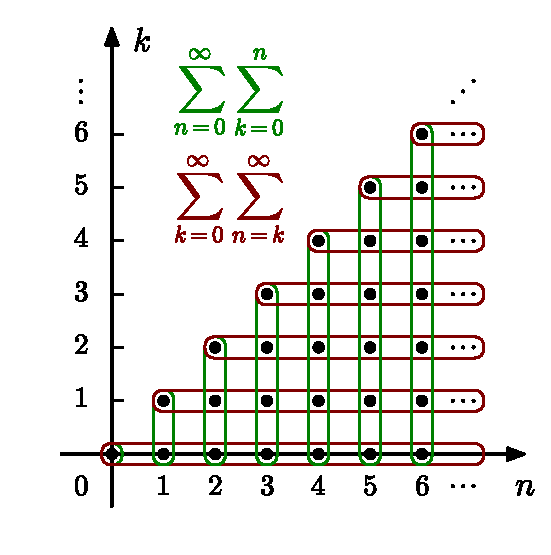
\includegraphics[width=\textwidth]{figuras/montmort_matching_double_summation.pdf}
  \end{minipage}\hfill
  \begin{minipage}[c]{0.5\textwidth}
    \caption{
       Equivalencia de dobles sumatorias cuando el par de valores \((n, k)\) consisten en los números naturales de la mitad del cuadrante.
    } \label{fig:montmort_matching_double_summation}
  \end{minipage}
\end{figure}
De las ecuaciones \ref{eq:match_phi_deduction_1} y \ref{eq:match_phi_deduction_2}, se deduce que la función generadora de momentos es
\[
 \phi(z)=\frac{e^{-z}}{1-z}.
\]
Además, puede demostrarse que
\begin{equation}\label{eq:match_generator_function}
 \frac{e^{-z}}{1-z}=\sum_{n=0}^{\infty}\left(\sum_{k=0}^{n}\frac{(-1)^k}{k!}\right)z^n.
\end{equation}
Para hacerlo, se procede de forma análoga a como se realizó con la deducción de la función generadora de momentos. Comenzando con el lado derecho de la igualdad y operando, se tiene que,
\begin{align*}
 \sum_{n=0}^{\infty}\left(\sum_{k=0}^{n}\frac{(-1)^k}{k!}\right)z^n
  &=\sum_{n=0}^{\infty}\sum_{k=0}^{n}\frac{(-1)^kz^{k}}{k!}z^{n-k}\\
  &=\sum_{k=0}^{\infty}\sum_{n=k}^{\infty}\frac{(-1)^kz^{k}}{k!}z^{n-k}\\
  &=\sum_{k=0}^{\infty}\frac{(-1)^kz^{k}}{k!}\sum_{n=k}^{\infty}z^{n-k}\\
  &=\sum_{k=0}^{\infty}\frac{(-1)^kz^{k}}{k!}\sum_{i=0}^{\infty}z^i\\
  &=e^{-z}\frac{1}{1-z},
\end{align*}
en donde en la última igualdad se tomó en cuenta que el primer factor del producto de sumatorias es la serie de potencias de \(e^{-z}\). Por lo tanto, se concluye que
\begin{equation*}
 \phi(z)=\frac{e^{-z}}{1-z}=\sum_{n=0}^{\infty}\left(\sum_{k=0}^{n}\frac{(-1)^k}{k!}\right)z^n.
\end{equation*}
Comparando esta ecuación con la ecuación \ref{eq:generating_moments_function}, se obtiene que la expresión de \(p_n(0)\) que se buscaba, 
\begin{equation}\label{eq:match_pn0}
 p_n(0)=\sum_{k=0}^{n}\frac{(-1)^k}{k!}.
\end{equation}
Notar que
\[
 e^{-z}=\sum_{n=0}^{\infty}\frac{(-1)^nz^n}{n!}\qquad\Rightarrow\qquad 
  e^{-1}=\sum_{n=0}^{\infty}\frac{(-1)^n}{n!}
\]
y por lo tanto,
\[
 \lim_{n\to\infty}p_n(0)=\frac{1}{e}.
\]
Finalmente, sustituyendo la ecuación \ref{eq:match_pn0} en la ecuación \ref{eq:match_pnk1} se obtiene la probabilidad de que exactamente \(k\) cartas de las \(n\) lleguen al destino correcto, y es
\[
 p_n(k)=\frac{1}{k!}\sum_{m=0}^{n-k}\frac{(-1)^m}{m!}.
\]
Con esto, queda completamente caracterizado el evento \(X_k\). La respuesta a la pregunta realizada inicialmente de cual es la probabilidad de que al menos una de las \(n\) cartas llegue al destino correcto es
\begin{align*}
 P\{\textrm{Al menos una carta llegue al destino correcto}\}&=1-p_n(0)\\
   &=1-\sum_{k=0}^{n}\frac{(-1)^k}{k!}\\
   &\to1-\frac{1}{e}\approx 0.63212056
\end{align*}

Además, como \(p_n(0)\) es la probabilidad de que no haya ninguna coincidencia en los \(n\) sobres, se calcula como el cociente entre la cantidad de permutaciones donde no hay ninguna coincidencia (desarreglos, \(!n\)), y la cantidad de permutaciones posibles,
\[
 p_n(0)=\frac{!n}{n!}
\]
y por lo tanto, la cantidad de desarreglos de \(n\) objetos es
\begin{equation}\label{eq:match_derangements}
 !n=n!\sum_{k=0}^{n}\frac{(-1)^k}{k!}.
\end{equation}


\subsection{Otras consideraciones}

El resultado de la ecuación \ref{eq:match_generator_function} puede obtenerse usando la siguiente propiedad de las funciones generadoras de momentos. Sean \(\phi_a(z)\) y \(\phi_b(z)\) las funciones generadoras de las variables aleatorias discretas \(X\) e \(Y\) respectivamente, con \(P\{X=n\}=a_n\) y \(P\{Y=n\}=b_n\) para \(-\infty<n<\infty\). La función generadora de \(c_n=(a*b)(n)\) es
\[
 \phi_c(z)=\phi_a(z)\phi_b(z)=\sum_{n=-\infty}^{\infty}c_nz^n,
\]
donde
\[
 c_n=(a*b)(n)=\sum_{k=-\infty}^{\infty}a_kb_{n-k},
\]
es la convolución entre las secuencias \(a_n\) y \(b_n\) \cite{miller2017probability_chap19}. Esto significa que la función generadora de la convolución de secuencias es el producto de las funciones generadoras de las secuencias. Tener en cuenta que en este contexto, una secuencia es la densidad de probabilidad de una variable aleatoria discreta. Este resultado proviene de la multiplicación de polinomios:
\[
  \textrm{si}\qquad
  \begin{array}{l} 
  \displaystyle f(x)=\sum_{n=-\infty}^{\infty}a_nx^n\\
  \displaystyle g(x)=\sum_{m=-\infty}^{\infty}b_nx^n \end{array}
  \qquad\Rightarrow\qquad 
  \begin{array}{l} 
  \displaystyle h(x)=f(x)g(x)=\sum_{n=-\infty}^{\infty}c_nx^n,\\
  \\
  \textrm{con}\qquad c_n=(a*b)(n). \end{array}
 \]
En el caso en que el soporte de la secuencias sean los naturales, es decir, \(n\geq0\), se cumple que
\[
 \phi_c(z)=\phi_a(z)\phi_b(z)=\sum_{n=0}^{\infty}c_nz^n,\qquad\textrm{con}\qquad c_n=(a*b)(n)=\sum_{k=0}^{n}a_kb_{n-k}.
\]
Teniendo esto en cuenta y volviendo a la ecuación \ref{eq:match_generator_function}, sean
\[
 \phi_a(z)=e^{-z}=\sum_{n=0}^{\infty}\frac{(-1)^nz^n}{n!}\qquad\textrm{y}\qquad 
 \phi_b(z)=\frac{1}{1-z}=\sum_{n=0}^{\infty}z^n,
\]
Las secuencias de estas funciones generadoras son
\[
 a_n=
 \left\{\begin{array}{ll}
  \dfrac{(-1)^n}{n!}, & \textrm{si }n\geq 0 \\
  0, & \textrm{si }n<0
 \end{array} \right.
 \qquad\textrm{y}\qquad
 b_n=
 \left\{\begin{array}{ll}
  1, & \textrm{si }n\geq 0 \\
  0, & \textrm{si }n<0
 \end{array}, \right.
\]
respectivamente. Por lo tanto, la secuencia de la función generadora
\[
 \phi_c(z)=\phi_a(z)\phi_b(z)=\frac{e^{-z}}{1-z}
\]
es
\[
 c_n=(a*b)(n)=\sum_{k=0}^{n}\frac{(-1)^k}{k!},
\]
ya que \(b_n\) es el escalón de Heaviside, y la convolución de una secuencia por un escalón de Heaviside es la suma acumulada de la secuencia. Se concluye que 
\[
 \phi_c(z)=\frac{e^{-z}}{1-z}=\sum_{n=0}^{\infty}\sum_{k=0}^{n}\frac{(-1)^k}{k!}z^n,
\]
de forma acorde con la ecuación \ref{eq:match_generator_function}

El problema de las parejas también puede resolverse recursivamente de la siguiente forma \cite{hathout2003old}. Sea \(D_n\) la cantidad de desarreglos de las \(n\) cartas (\(D_n\equiv\,!n\)), es decir, la cantidad de formas posibles que se pueden poner las cartas en los sobres de forma de que no haya ninguna coincidencia. Llámese carta 1 a la primera carta. Hay \(n-1\) formas posibles de poner la carta en un sobre sin que haya coincidencia. Supóngase que la carta 1 se pone en el sobre \(i\), con \(i\neq 1\). Ahora se consideran dos casos: \(a)\) la carta correspondiente al sobre \(i\) se guarda en el sobre 1, y \(b)\) la carta del sobre \(i\) se guarda en otro sobre distinto del 1. Entonces,
\begin{enumerate}[\(a)\)]
 \item el resto de las \(n-2\) cartas se guarda en un sobre incorrecto, y la cantidad de formas posibles de hacerlo es \(D_{n-2}\).
 \item cada una de las \(n-1\) cartas tiene una opción prohibida. La opción prohibida de la carta \(i\) es el sobre 1, y la opción prohibida de las otras cortas es su propio sobre. Por lo tanto, la cantidad de formas posibles de guardar las \(n-1\) cartas sin que haya coincidencia en estas condiciones es \(D_{n-1}\).
\end{enumerate}
Como los eventos \(a)\) y \(b)\) son mutuamente excluyentes y abarcan todas las posibiidades, se cumple que
\[
 D_n=(n-1)\left(D_{n-1}+D_{n-2}\right).
\]
Además, se tiene como condiciones iniciales que \(D_0=1\) y \(D_1=0\). Ahora, la probabilidad de que no haya ninguna coincidencia es
\begin{align*}
 P_n&=\frac{D_n}{n!}\\
  &=\frac{n-1}{n!}\left(D_{n-1}+D_{n-2}\right)\\
  &=(n-1)\left[\frac{D_{n-1}}{n(n-1)!}+\frac{D_{n-2}}{n(n-1)(n-2)!}\right]\\
  &\overset{(a)}{=}(n-1)\left[\frac{P_{n-1}}{n}+\frac{P_{n-2}}{n(n-1)}\right]\\
  &=\left(1-\frac{1}{n}\right)P_{n-1}+\frac{1}{n}P_{n-2},
\end{align*}
donde en \((a)\) se usó que \(P_k=D_k/k!\). Finalmente, se obtiene que
\[
 P_n=P_{n-1}-\frac{1}{n}\left(P_{n-1}-P_{n-2}\right)
\]
con las condiciones iniciales \(P_0=1\) y \(P_1=0\). Resolviendo recursivamente, se ve que
\begin{align*}
 P_2&=P_1-\frac{1}{2}\left(P_1-P_0\right)=0+\frac{1}{2}=\frac{1}{2!}\\
 P_3&=P_2-\frac{1}{3}\left(P_2-P_1\right)=\frac{1}{2!}-\frac{1}{3}\times\frac{1}{2}=\frac{1}{2!}-\frac{1}{3!}\\
 P_4&=P_3-\frac{1}{4}\left(P_3-P_2\right)=\frac{1}{2!}-\frac{1}{3!}+\frac{1}{4}\times\frac{1}{3!}=\frac{1}{2!}-\frac{1}{3!}+\frac{1}{4!}\\
 \vdots&\\
 P_n&=\frac{1}{2!}-\frac{1}{3!}+\frac{1}{4!}-\frac{1}{5!}+\dots+\frac{(-1)^n}{n!},
\end{align*}
es decir,
\[
 P_n=\sum_{k=2}^{n}\frac{(-1)^k}{k!}=\sum_{k=0}^{n}\frac{(-1)^k}{k!},
\]
en concordancia con el resultado obtenido mediante la función generadora de momentos de la ecuación \ref{eq:match_pn0}, y
\[
 D_n=n!P_n=n!\sum_{k=0}^{n}\frac{(-1)^k}{k!}.
\]

\chapter{Dos variables aleatorias}

Continuando con el estudio del libro \cite{papoulis2002probability}, en lo que sigue se incluye lo desarrollado en el capítulo 6.

\section{Algunas definiciones y propiedades}

Se incluyen a continuación algunas definiciones y propiedades debido a que serán mencionadas mas adelante.

\subsection{Distribución de probabilidad conjunta}

La distribución de probabilidad conjunta \(F_{xy}(x,\,y)\), o simplemente \(F(x,\,y)\), de dos variables aleatorias \(\x\) e \(\y\) es la probabilidad del evento
\[
 \{\x\leq x,\, \y\leq y\}=\{(\x,\,\y)\in D_1\}
\]
donde \(x\) e \(y\) son dos números reales arbitrarios y \(D_1\) es el cuadrante mostrado en la figura \ref{fig:joint_distribution_region}. Entonces,
\[
 F(x,\,y)=P\{\x\leq x,\, \y\leq y\}.
\]
\begin{figure}[!htb]
\begin{center}
  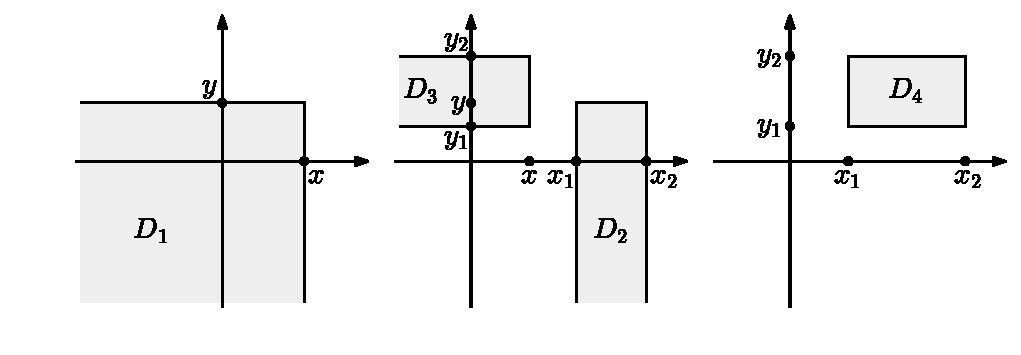
\includegraphics[width=0.85\textwidth]{figuras/joint_distribution_region_v2.pdf}
  \caption{
       Regiones del plano \(xy\) correspondientes a distintos eventos. La gráfica de la izquierda resalta los puntos del plano del evento \(\{\x\leq x,\, \y\leq y\}=\{(\x,\,\y)\in D_1\}\). En la gráfica del centro, la semi-banda vertical \(D_2\) son los puntos del plano del evento \(\{x_1<\x\leq x_2,\,\y\leq y\}\) y la semi-banda horizontal \(D_3\) son los puntos del plano del evento \(\{\x\leq x,\,y_1<\y\leq y_2\}\). La gráfica de la derecha consiste en los puntos de la región \(D_4\), correspondiente al evento \(\{x_1<\x\leq x_2,\,y_1<\y\leq y_2\}\).
    } \label{fig:joint_distribution_region}
\end{center}
\end{figure}

La distribución de probabilidad cumple las siguientes propiedades:
\begin{enumerate}[1.]
 \item La función \(F_{xy}(x,\,y)\) es tal que
 \[
  F(-\infty,\,y)=0,\qquad F(x,\,-\infty)=0,\qquad F(\infty,\,\infty)=1.
 \]
 Demostración: las dos primeras igualdades indican que
 \begin{equation}\label{eq:joint_distribution_properties1}
 \begin{aligned}
    F(-\infty,\,y)&=P\{\x=-\infty,\,\y\leq y\}=0\\
    F(x,\,-\infty)&=P\{\x\leq x,\,\y=-\infty\}=0.
 \end{aligned}
 \end{equation}
 Como se cumple que
 \[
  P\{\x=-\infty\}=P\{\y=-\infty\}=0
 \]
 y además
 \[
  \{\x=-\infty,\,\y\leq y\}\subset \{\x=-\infty\},\qquad \{\x\leq x,\,\y=-\infty\}\subset \{\y=-\infty\},
 \]
 queda demostrada la ecuación \ref{eq:joint_distribution_properties1}. La última igualdad surge de que
 \[
  F(\infty,\,\infty)=P\{\x\leq\infty,\,\y\leq \infty\},
 \]
 y de observar que 
 \[
  \{\x\leq\infty,\,\y\leq \infty\}=S, \qquad P(S)=1,
 \]
 es decir, el evento \(\{\x\leq\infty,\,\y\leq \infty\}\) es todo el espacio muestral, y por lo tanto, su probabilidad de ocurrencia es 1.
 \item El evento \(\{x_1<\x\leq x_2,\,\y\leq y\}\) consiste en todos los puntos \((\x,\,\y)\) en la semi-banda vertical \(D_2\) y el evento \(\{\x\leq x,\,y_1<\y\leq y_2\}\) consiste en todos los puntos \((\x,\,\y)\) en la semi-banda horizontal \(D_3\) en la figura \ref{fig:joint_distribution_region}. La probabilidad de estos eventos es
 \begin{equation}\label{eq:joint_distribution_properties2}
 \def\arraystretch{1.2}
 \begin{array}{lll}
    P\{x_1<\x\leq x_2,\,\y\leq y\}&=&F(x_2,\,y)-F(x_1,\,y)\\
    P\{\x\leq x,\,y_1<\y\leq y_2\}&=&F(x,\,y_1)-F(x,\,y_2).
 \end{array}
 \end{equation} 
Demostración: observando que
\[
 \{\x\leq x_2,\,\y\leq y\}=\{\x\leq x_1,\,\y\leq y\}\cup\{x_1<\x\leq x_2,\,\y\leq y\},
\]
y teniendo en cuenta que los eventos a la derecha de la igualdad son mutuamente excluyentes, se cumple que
\[
 P\{\x\leq x_2,\,\y\leq y\}=P\{\x\leq x_1,\,\y\leq y\}+P\{x_1<\x\leq x_2,\,\y\leq y\},
\]
y por lo tanto
\begin{align*}
 P\{x_1<\x\leq x_2,\,\y\leq y\}&=P\{\x\leq x_2,\,\y\leq y\}-P\{\x\leq x_1,\,\y\leq y\}\\
   &=F(x_2,\,y)-F(x_1,\,y),
\end{align*}
que es lo que se quería demostrar. La segunda igualdad en la ecuación \ref{eq:joint_distribution_properties2} se demuestra de forma análoga.
\item Se cumple que
\begin{equation}\label{eq:joint_distribution_rectangular_region}
  P\{x_1<\x\leq x_2,\,y_1<\y\leq y_2\}=F(x_2,\,y_2)-F(x_1,\,y_2)-F(x_2,\,y_1)+F(x_1,\,y_1),
\end{equation}
que es la probabilidad de que \((\x,\,\y)\) esté en el rectángulo \(D_4\) de la figura \ref{fig:joint_distribution_region}
Demostración: Como
\[
 \{x_1<\x\leq x_2,\,\y\leq y_2\}=\{x_1<\x\leq x_2,\,\y\leq y_1\}\cup\{x_1<\x\leq x_2,\,y_1<\y\leq y_2\}
\]
y los eventos a la derecha de la igualdad son mutuamente excluyentes, se cumple que
\[
 P\{x_1<\x\leq x_2,\,\y\leq y_2\}=P\{x_1<\x\leq x_2,\,\y\leq y_1\}+P\{x_1<\x\leq x_2,\,y_1<\y\leq y_2\}.
\]
Por lo tanto,
\begin{align*}
 P\{x_1<\x\leq x_2,\,y_1<\y\leq y_2\}=&P\{x_1<\x\leq x_2,\,\y\leq y_2\}-P\{x_1<\x\leq x_2,\,\y\leq y_1\}\\
  \overset{(a)}{=}&\left(F(x_2,\,y_2)-F(x_1,\,y_2)\right)-\left(F(x_2,\,y_1)-F(x_1,\,y_1)\right)\\
  =&F(x_2,\,y_2)-F(x_1,\,y_2)-F(x_2,\,y_1)+F(x_1,\,y_1),
\end{align*}
donde en \((a)\) se usó la primera ecuación en \ref{eq:joint_distribution_properties2}.
\end{enumerate}

\subsection{Densidad de probabilidad conjunta}
La densidad de probabilidad conjunta de \(\x\) e \(\y\) es por definición la función
\begin{equation}\label{eq:joint_density_definition}
 f(x,\,y)=\frac{\partial^2F(x,\,y)}{\partial x\partial y}.
\end{equation}
Se cumple por lo tanto que
\[
 F(x,\,y)=\int_{-\infty}^{x}\int_{-\infty}^{y}f(\alpha,\,\beta)\,d\alpha\,d\beta.
\]
De esta forma,
\[
 F(-\infty,\,y)=0\qquad\textrm{y}\qquad F(x,\,-\infty)=0,
\]
acorde con una de las propiedades de la distribución de probabilidad conjunta.

\subsection{Estadísticas conjuntas}
Se puede demostrar que la probabilidad de que el punto \((\x,\,\y)\) esté en una región \(D\) del plano \(xy\) es la integral de \(f(x,\,y)\) en \(D\), es decir,
\begin{equation}\label{eq:joint_probability_definition}
 P\{(\x,\,\y)\in D\}=\iint_{D} f(x,\,y)\,dx\,dy.
\end{equation}

\subsection{Estadísticas marginales}\label{sec:marginal_statisctics_two_rv}
En el análisis de varias variables aleatorias, la estadística de cada una por separado se llama \emph{marginal}. De esta forma, \(F_x(x)\) es la \emph{distribución marginal} y \(f_x(x)\) es la \emph{densidad marginal} de \(\x\). Se puede demostrar que la estadística marginal de \(\x\) e \(\y\) en función de su estadística conjunta \(F(x,\,y)\) y \(f(x,\,y)\) es
\[
 F_x(x)=F(x,\,\infty),\qquad F_y(y)=F(\infty,\,y)
\]
\begin{equation}\label{eq:marginal_densities_definition}
 f_x(x)=\int_{-\infty}^{\infty}f(x,\,y)\,dy,\qquad f_y(y)=\int_{-\infty}^{\infty}f(x,\,y)\,dx.
\end{equation}

\subsection{Independencia}\label{sec:independence}

En la sección \ref{sec:independents_events} se definió independencia de eventos. Se dice que dos variables aleatorias son \emph{independientes} si los eventos \(\{\x\in A\}\) y \(\{\y\in B\}\) son independientes, es decir,
\[
 P\{\x\in A,\,\y\in B\}=P\{\x\in A\}P\{\y\in B\},
\]
donde \(A\) y \(B\) son dos conjuntos arbitrarios en los ejes \(x\) e \(y\) respectivamente. Aplicando esto a los eventos \(\{\x\leq x\}\) y \(\{\y\leq y\}\), se concluye que si \(\x\) e \(\y\) son independientes, se cumple que
\begin{equation}\label{eq:independent_rv_distribution}
 F(x,\,y)=F_x(x)F_y(y),
\end{equation}
y por lo tanto, también se cumple que
\begin{equation}\label{eq:independent_rv_density}
 f(x,\,y)=f_x(x)f_y(y).
\end{equation}
Puede demostrarse a partir de la ecuación \ref{eq:joint_probability_definition} que lo recíproco también es cierto: si se cumple la ecuación \ref{eq:independent_rv_distribution} o \ref{eq:independent_rv_density}, las variables aleatorias \(\x\) e \(\y\) son independientes.

\paragraph{Ejemplo: la aguja de Buffon.} Un plano tiene dibujadas rectas paralelas separadas una distancia \(d\), y se tira de forma aleatoria una aguja de largo \(l\) sobre el. Se quiere averiguar la probabilidad de que la aguja intersecte alguna recta. Este problema fue propuesto por el naturalista francés Georges-Louis Leclerc, conde de Buffon, en 1733 y publicado por el en 1777 con la solución\footnote{Fuente: \url{http://mathworld.wolfram.com/BuffonsNeedleProblem.html}}.

\textbf{Solución:} sea \(z\) la distancia entre el centro de la aguja y la recta mas cercana y sea \(\theta\) el ángulo entre la aguja y la recta. El hecho de que la aguja sea tirada de forma aleatoria permite asumir que:
\begin{itemize}
 \item \(z\) es una variable aleatoria uniformemente distribuida en \([0,\,d/2]\), por lo que su densidad de probabilidad es
 \[
  f_z(z)=\left\{\begin{array}{ll}
  2/d, &  \textrm{si}\quad0\leq z\leq d/2\\
  0, & \textrm{en otro caso.}
 \end{array} \right.
 \]
 \item \(\theta\) es una variable aleatoria uniformemente distribuida en \([0,\,\pi/2]\), por lo que su densidad de probabilidad es
 \[
  f_\theta(\theta)=\left\{\begin{array}{ll}
  2/\pi, &  \textrm{si}\quad0\leq\theta\leq \pi/2\\
  0, & \textrm{en otro caso.}
 \end{array} \right.
 \]
 De forma equivalente, se podría haber considerado que \(0\leq\theta\leq\pi\) con densidad de probabilidad \(f_\theta=1/\pi\), pero las probabilidades de \(\theta\) en los intervalos \([0,\,\pi/2]\) y \([\pi/2,\,\pi]\) son simétricas, por lo que alcanza considerar solo el intervalo \([0,\,\pi/2]\) con el doble de probabilidad.
 \item \(z\) y \(\theta\) son variables aleatorias independientes, y por lo tanto se cumple que
 \[
  f_{z\theta}(z,\,\theta)=f_z(z)f_\theta(\theta)
  =\left\{\begin{array}{ll}
  4/\pi d, &  \textrm{si}\quad0\leq z\leq d/2\quad\textrm{y}\quad0\leq\theta\leq \pi/2\\
  0, & \textrm{en otro caso.}
 \end{array} \right.
 \]
\end{itemize}
Según estas especificaciones, el espacio muestral del experimento es
\[
 \Omega=\left\{(z,\,\theta)\,:\,0\leq z\leq\frac{d}{2},\,0\leq\theta\leq\frac{\pi}{2}\right\}.
\]
Para encontrar la probabilidad de intersección hay que separar los casos \(l\leq d\) y \(l>d\). Se comenzará resolviendo el primero.

Como se observa en el caso límite de la figura \ref{fig:buffon_needle_short}, si \(l\leq d\), la aguja intersecta una recta si se cumple que
\[
 z\leq\frac{l}{2}\sin{\theta}.
\]
Llámese \(D\) a esta región del plano \((z,\,\theta)\), es decir,
\[
 D=\left\{(z,\,\theta)\,:\,0\leq z\leq\frac{l}{2}\sin{\theta},\,0\leq\theta\leq\frac{\pi}{2}\right\}.
\]
La probabilidad de intersección es
\begin{align*}
 P\{\textrm{intersección}\}&=\iint_{D}f_{z\theta}(z,\,\theta)\,dz\,d\theta\\
  &=\int_{0}^{\pi/2}\int_{0}^{(l/2)\sin\theta}\frac{4}{\pi d}\,dz\,d\theta\\
  &=\frac{4}{\pi d}\int_{0}^{\pi/2}\left(z\,\bigg|_{0}^{(l/2)\sin\theta}\right)\,d\theta\\
  &=\frac{4}{\pi d}\int_{0}^{\pi/2}\frac{l}{2}\sin\theta\,d\theta\\
  &=\frac{2l}{\pi d}\left(-\cos\theta\,\bigg|_{0}^{\pi/2}\right)\\
  &=\frac{2l}{\pi d}\left(-\cos\frac{\pi}{2}+1\right),
\end{align*}
concluyendo que
\[
 P\{\textrm{intersección}\}=\frac{2l}{\pi d}.
\]
\begin{figure}[!htb]
  \begin{minipage}[c]{0.45\textwidth}
    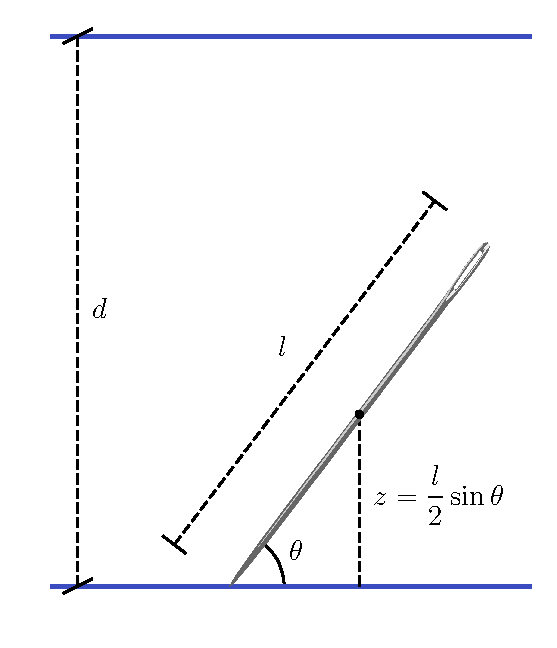
\includegraphics[width=\textwidth]{figuras/buffon_needle_short.pdf}
  \end{minipage}\hfill
  \begin{minipage}[c]{0.45\textwidth}
    \caption{
       Experimento de la aguja de Buffon para el caso en que el largo \(l\) de la aguja es menor que la distancia \(d\) entre las líneas del plano. La condición para que la aguja intersecte una recta del plano, es que la distancia \(z\) entre el centro de la aguja y la recta mas cercana sea menor a \((l/2)\sin\theta\), donde \(\theta\) es el ángulo entre la aguja y las rectas del plano. En la figura se muestra el caso especial en que \(z=(l/2)\sin\theta\).
    } \label{fig:buffon_needle_short}
  \end{minipage}
\end{figure}

Una aplicación interesante de este experimento es en la estimación del valor de \(\pi\). Supóngase que se arroja la aguja \(n\) veces, y de esas \(n\) veces \(h\) veces intersecta una recta del plano. Empleando la interpretación frecuentista del concepto de probabilidad, se cumple que
\[
 P\{\textrm{intersección}\}=\frac{2l}{\pi d}\approx\frac{h}{n},
\]
por lo que el valor de \(\pi\) puede estimarse como
\[
 \pi\approx\frac{2ln}{dh}.
\]
En 1901, el matemático italiano Mario Lazzarini realizó el experimento de la aguja de Buffon. Lazzarini arrojo una aguja \(n=3408\) veces y obtuvo la estimación de \(\pi\) de \(355/113=3,14159292\), correcta hasta 6 digitos después de la coma. Esta estimación es demasiado precisa para la baja cantidad \(n\) de veces que repitió el experimento debido a que concía el valor de \(\pi\) y realizó el experimento de forma sesgada para obtener un buen resultado\footnote{Ver \url{https://en.wikipedia.org/wiki/Buffon\%27s_needle_problem\#Estimating_\%CF\%80}}. De todas formas, el experimento realizado por Lazzarini es considerado la primer aplicación de la técnica de integración de Montecarlo.

Se calculará a continuación la probabilidad de intersección para el caso en que la aguja es mas larga que la separación de los renglones en el plano, es decir, \(l>d\). Para hacerlo, se comienza considerando el caso límite en que los extremos de la aguja tocan sin cortar dos rectas sucesivas, como se muestra en la figura \ref{fig:buffon_needle_long}. En ese caso, \(z=d/2\) y
\[
 \sin\theta=\frac{d}{l}\qquad\Rightarrow\qquad\theta=\arcsin\frac{d}{l}.
\]
Se deduce entonces que si \(\theta\geq\arcsin d/l\), la aguja va a intersectar al menos una recta, independientemente del valor de \(z\). La región del plano \((z,\,\theta)\) de esta situación es
\[
 D_1=\left\{(z,\,\theta)\,:\,0\leq z\leq\frac{d}{2},\,\arcsin\frac{d}{l}\leq\theta\leq\frac{\pi}{2}\right\}.
\]
En el caso en que \(\theta<\arcsin d/l\), la aguja intersecta una recta si \(z\leq(l/2)\sin\theta\), como se muestra también en la figura \ref{fig:buffon_needle_long}, y la región del plano \((z,\,\theta)\) de esta situación es
\[
 D_2=\left\{(z,\,\theta)\,:\,0\leq z\leq\frac{l}{2}\sin\theta,\,0\leq\theta<\arcsin\frac{d}{l}\right\}.
\]
\begin{figure}[!htb]
\begin{center}
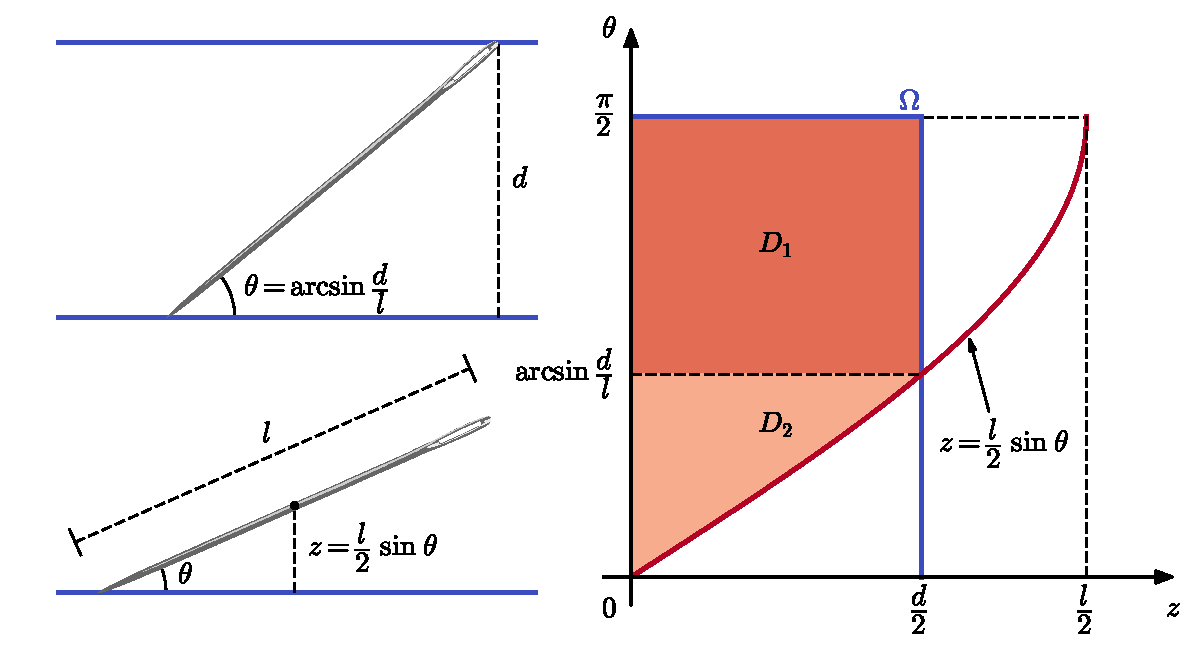
\includegraphics[width=0.9\textwidth]{figuras/buffon_needle_long.pdf}
\caption{\label{fig:buffon_needle_long} Experimento de la aguja de Buffon para el caso en que el largo \(l\) de la aguja es mayor que la distancia \(d\) entre las líneas del plano. Si el ángulo de la aguja cumple que \(\theta\geq\arcsin d/l\), la aguja intersecta al menos una recta del plano. Esa situación consiste en los puntos \((z,\,\theta)\) en la región \(D_1\) del espacio muestral \(\Omega\). En el caso en que \(\theta<\arcsin d/l\), la aguja intersecta una recta si \(z\leq(l/2)\sin\theta\). Esta situación consiste en los puntos de la región \(D_2\).}
\end{center}
\end{figure}
Teniendo en cuenta que las regiones \(D_1\) y \(D_2\) son disjuntas (ver figura \ref{fig:buffon_needle_long}), la probabilidad de intersección es
\[
 P\{\textrm{intersección}\}=\iint_{D_1\cup D_2}f_{z\theta}(z,\,\theta)\,dz\,d\theta
 =\iint_{D_1}f_{z\theta}(z,\,\theta)\,dz\,d\theta+\iint_{D_2}f_{z\theta}(z,\,\theta)\,dz\,d\theta.
\]
La primera integral de la suma es
\begin{align*}
 \iint_{D_1}f_{z\theta}(z,\,\theta)\,dz\,d\theta&=\int_{\arcsin d/l}^{\pi/2}\int_{0}^{d/2}\frac{4}{\pi d}\,dz\,d\theta\\
 &=\frac{4}{\pi d}\int_{\arcsin d/l}^{\pi/2}\left(z\,\bigg|_{0}^{d/2}\right)\,d\theta\\
 &=\frac{4}{\pi d}\int_{\arcsin d/l}^{\pi/2}\frac{d}{2}\,d\theta\\
 &=\frac{2}{\pi}\left(\theta\,\bigg|_{\arcsin d/l}^{\pi/2}\right)\\
 &=\frac{2}{\pi}\left(\frac{\pi}{2}-\arcsin\frac{d}{l}\right),
\end{align*}
y la segunda es
\begin{align*}
 \iint_{D_2}f_{z\theta}(z,\,\theta)\,dz\,d\theta&=\int_{0}^{\arcsin d/l}\int_{0}^{(l/2)\sin\theta}\frac{4}{\pi d}\,dz\,d\theta\\
 &=\frac{4}{\pi d}\int_{0}^{\arcsin d/l}\left(z\,\bigg|_{0}^{(l/2)\sin\theta}\right)\,d\theta\\
 &=\frac{4}{\pi d}\int_{0}^{\arcsin d/l}\frac{l}{2}\sin\theta\,d\theta\\
 &=\frac{2l}{\pi d}\left(-\cos\theta\bigg|_{0}^{\arcsin d/l}\right)\\
 &=\frac{2l}{\pi d}\left[1-\cos\left(\arcsin\frac{d}{l}\right)\right]\\
 &\overset{(a)}{=}\frac{2l}{\pi d}\left[1-\sqrt{1-\sin^2\left(\arcsin\frac{d}{l}\right)}\right]\\
 &=\frac{2l}{\pi d}\left(1-\sqrt{1-\frac{d^2}{l^2}}\right)\\
 &=\frac{2}{\pi d}\left(l-\sqrt{l^2-d^2}\right),
\end{align*}
donde en \((a)\) se empleó la identidad \(\sin^2\theta+\cos^2\theta=1\).
Combinando ambos resultados se obtiene que
\begin{align*}
 P\{\textrm{intersección}\}&=\frac{2}{\pi}\left(\frac{\pi}{2}-\arcsin\frac{d}{l}\right)+\frac{2}{\pi d}\left(l-\sqrt{l^2-d^2}\right)\\
 &=\frac{2}{\pi d}\left(\frac{\pi d}{2}-d\arcsin\frac{d}{l}+l-\sqrt{l^2-d^2}\right).
\end{align*}


\subsection{Variables aleatorias conjuntamente normales}\label{sec:joint_normal_pdf}

Se dice que dos variables aleatorias \(\x\) e \(\y\) son conjuntamente normales si su densidad de probabilidad conjunta es
\begin{equation}\label{eq:joint_normal_pdf1}
 f(x,\,y)=A\exp\left\{-\frac{1}{2(1-r^2)}\left[\frac{(x-\eta_1)^2}{\sigma_1^2}-2r\frac{(x-\eta_1)(y-\eta_2)}{\sigma_1\sigma_2}+\frac{(y-\eta_2)^2}{\sigma_2^2}\right]\right\},
\end{equation}
con
\begin{equation}\label{eq:joint_normal_pdf2}
 A=\frac{1}{2\pi\sigma_1\sigma_2\sqrt{1-r^2}},\qquad|r|<1.
\end{equation}
La función \(f(x,\,y)\) es una exponencial de exponente negativo si \(|r|<1\), es positiva para todo \((x,\,y)\), e integra a 1, como se mostrará a continuación. Se denota como
\[
 N(\eta_1,\,\eta_2,\,\sigma_1^2,\,\sigma_2^2,\,r).
\]
Como se verá, \(\eta_1\) y \(\eta_2\) son los valores esperados de \(\x\) e \(\y\) respectivamente, y \(\sigma_1^2\) y \(\sigma_2^2\) sus varianzas. El parámetro \(r\) se llama coeficiente de correlación, y su significado será explicado mas adelante.

Se demostrará que las densidades marginales de \(\x\) e \(\y\) son
\[
 f_x(x)=\frac{1}{\sigma_1\sqrt{2\pi}}\,e^{-(x-\eta_1)^2/2\sigma_1^2}\qquad
 f_y(y)=\frac{1}{\sigma_2\sqrt{2\pi}}\,e^{-(y-\eta_2)^2/2\sigma_2^2},
\]
es decir, \(\x\) e \(\y\) son variables aleatorias normales con \(\x\sim N(\eta_1,\,\sigma_1^2)\) y \(\y\sim N(\eta_2,\,\sigma_2^2)\). Para esto, hay que probar que si se integra la ecuación \ref{eq:joint_normal_pdf1} respecto a \(x\) se obtiene \(f_y(y)\), como indica la ecuación \ref{eq:marginal_densities_definition}, y si se integra respecto a \(y\) se obtiene \(f_x(x)\). Se parte observando que el término entre paréntesis rectos del exponente en \ref{eq:joint_normal_pdf1} se puede escribir como
\[
 \frac{(x-\eta_1)^2}{\sigma_1^2}-2r\frac{(x-\eta_1)(y-\eta_2)}{\sigma_1\sigma_2}+\frac{(y-\eta_2)^2}{\sigma_2^2}
 =\left(\frac{x-\eta_1}{\sigma_1}-r\frac{y-\eta_2}{\sigma_2}\right)^2+(1-r^2)\frac{(y-\eta_2)^2}{\sigma_2^2}
\]
es decir, como un cuadrado perfecto y un segundo sumando para mantener la igualdad. Observando el lado derecho de la igualdad, se ve que si \(|r|<1\), la expresión es positiva, y por lo tanto, el exponente de la ecuación \ref{eq:joint_normal_pdf1} es negativo, como se mencionó previamente. Sacando denominador común \(\sigma_1\) en el primer sumando a la derecha de la igualdad, se llega a que el término entre paréntesis rectos del exponente en \ref{eq:joint_normal_pdf1} queda
\begin{equation}\label{eq:joint_normal_pdf_exponent}
 \left\{\frac{x-\left[\eta_1+r\frac{\sigma_1}{\sigma_2}(y-\eta_2)\right]}{\sigma_1}\right\}^2+(1-r^2)\frac{(y-\eta_2)^2}{\sigma_2^2}
\end{equation}
y definiendo 
\[
 \eta\triangleq \eta_1+r\frac{\sigma_1}{\sigma_2}(y-\eta_2),
\]
se tiene que la densidad marginal de \(\y\) es
\begin{align*}
 f_y(y)&=\int_{-\infty}^{\infty}f(x,\,y)\,dx\\
   &=\int_{-\infty}^{\infty}A\exp\left[-\frac{(x-\eta)^2}{2(1-r^2)\sigma_1^2}-\frac{(y-\eta_2)^2}{2\sigma_2^2}\right]\,dx\\
   &=A\,e^{-(y-\eta_2)^2/2\sigma_2^2} \int_{-\infty}^{\infty} e^{-(x-\eta)^2/2(1-r^2)\sigma_1^2}\,dx.
\end{align*}
La integral en la última igualdad representa una variable aleatoria normal de media \(\eta\) y varianza \(2(1-r^2)\sigma_1^2\) y por lo tanto, integra a \(\sqrt{2\pi(1-r^2)\sigma_1^2}\). Se llega al mismo resultado considerando que se trata de una integral gaussiana y aplicando la ecuación \ref{eq:random_gaussian_integral_with_sigma}. Teniendo en cuenta este resultado y sustituyendo el valor de A dado por la ecuación \ref{eq:joint_normal_pdf2}, se tiene que
\begin{align*}
 f_y(y)&=\frac{\sigma_1\sqrt{2\pi(1-r^2)}}{2\pi\sigma_1\sigma_2\sqrt{1-r^2}}\,e^{-(y-\eta_2)^2/2\sigma_2^2},
\end{align*}
concluyendo que 
\[
 f_y(y)=\frac{1}{\sigma_2\sqrt{2\pi}}\,e^{-(y-\eta_2)^2/2\sigma_2^2},
\]
que era lo que se quería demostrar. La densidad marginal de \(\x\) se obtiene de forma análoga. Como \(f_y(y)\) es una densidad de probabilidad normal, integra a 1. Por lo tanto, la integral doble de \(f(x,\,y)\) es 1 con el valor de \(A\) indicado en la ecuación \ref{eq:joint_normal_pdf2}, como se mencionó antes.

Vale la pena tener en cuenta las siguientes consideraciones:
\begin{itemize}
 \item Si dos variables aleatorias son conjuntamente normales, sus marginales son normales, como se acaba de mostrar.  Sin embargo, lo recíproco no es cierto: dos variables aleatorias que tienen marginales normales, no necesariamente son conjuntamente normales.
 \item La definición de variables aleatorias conjuntamente normales puede plantearse también de la siguiente forma: dos variables aleatorias \(\x\) e \(\y\) son conjuntamente normales si la suma \(a\x+b\y\) es normal para todo \(a\) y \(b\).
\end{itemize}

\section{Función de dos variables aleatorias}

Dadas dos variables aleatorias \(\x\) e \(\y\) y una función \(g(x,\,y)\), se construye una nueva variable aleatoria \(\z\) como
\[
 \z=g(\x,\,\y).
\]
A continuación se verá como calcular la densidad de probabilidad \(f_z(z)\) de \(\z\) a partir de la densidad de probabilidad conjunta \(f_{xy}(x,\,y)\) de \(\x\) e \(\y\). De forma general, se tiene que
\begin{align}\label{eq:pdf_of_funcion_of_two_rv}
 F_z(z)&=P\{\z\leq z\}=P\{g(\x,\,\y)\leq z\}=P\{(\x,\,\y)\in D_z\}\nonumber\\
   &=\iint_{(x,\,y)\in D_z}f_{xy}(x,\,y)\,dx\,dy,
\end{align}
donde \(D_z\) es la región del plano \(xy\) donde se cumple que \(g(x,\,y)\leq z\).

\subsection{\texorpdfstring{Ejemplo: Densidad de probabilidad de \(\z=\x+\y\)}{}}\label{sec:rv_sum_density}

Sea \(\z=\x+\y\). Se quiere determinar \(f_z(z)\). Se parte determinando la región \(D_z\) del plano \(xy\) en la ecuación \ref{eq:pdf_of_funcion_of_two_rv}, que en este caso es \(x+y\leq z\) y corresponde a la región del plano a la izquierda de la recta \(x+y=z\), como se muestra en la figura \ref{fig:joint_distribution_region_rv_sum}. Integrando sobre una banda a lo largo del eje \(x\) desde \(-\infty\) a \(x=z-y\) y luego desplazando la banda a lo largo del eje \(y\) desde \(-\infty\) a \(\infty\), se cubre toda la región. Por lo tanto,
\[
 F_z(z)=\int_{-\infty}^{\infty}\int_{-\infty}^{z-y}f_{xy}(x,\,y)\,dx\,dy.
\]
\begin{figure}[!htb]
\begin{center}
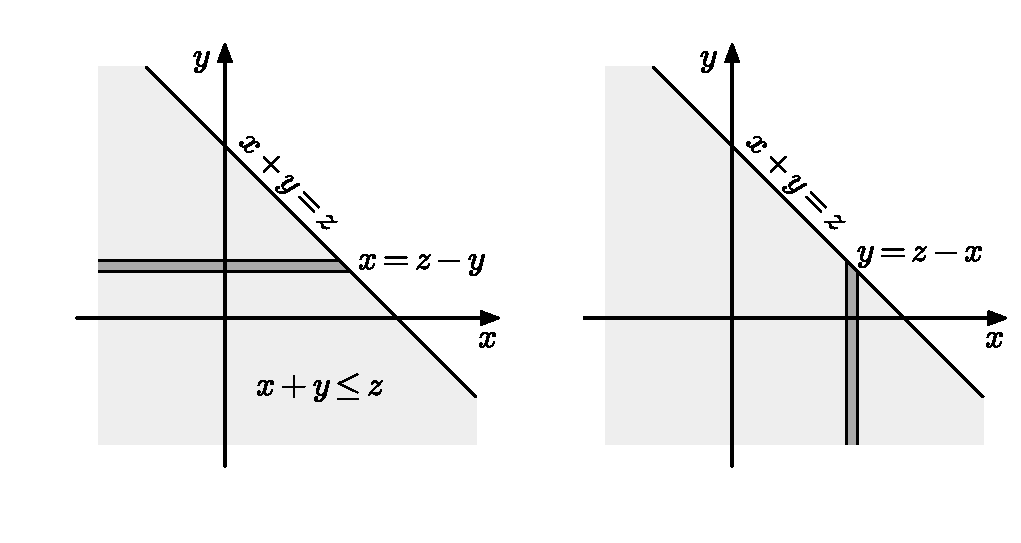
\includegraphics[width=0.75\columnwidth]{figuras/joint_distribution_region_rv_sum.pdf}
\caption{\label{fig:joint_distribution_region_rv_sum} Región de integración para determinar la densidad de probabilidad de \(\z=\x+\y\). La región de integración puede cubrirse de dos formas: \(i)\) integrando sobre una banda a lo largo del eje \(x\) desde \(-\infty\) a \(x=z-y\) y luego desplazando la banda a lo largo del eje \(y\) desde \(-\infty\) a \(\infty\), como se muestra en la gráfica de la izquierda, o \(ii)\) integrando sobre una banda a lo largo del eje \(y\) desde \(-\infty\) a \(y=z-x\) y luego desplazando la banda a lo largo del eje \(x\) desde \(-\infty\) a \(\infty\), como se muestra en la gráfica de la derecha.}
\end{center}
\end{figure}

Para calcular la densidad de probabilidad \(f_z(z)\) hay que diferenciar \(F_z(z)\) respecto a \(z\). Para esto, hay que aplicar la regla de integración de Leibnitz, que indica que si
\begin{equation}\label{eq:leibnitz_integration_rule1}
 F_z(z)=\int_{a(z)}^{b(z)}f(x,\,z)\,dx,
\end{equation}
la derivada es
\begin{equation}\label{eq:leibnitz_integration_rule2}
 \frac{dF_z(z)}{dz}=\frac{db(z)}{dz}f(b(z),\,z)-\frac{da(z)}{dz}f(a(z),\,z)+\int_{a(z)}^{b(z)}\frac{\partial f(x,\,z)}{\partial z}\,dx.
\end{equation}
Por lo tanto
\begin{align*}
 f_z(z)=\frac{dF_z(z)}{dz}&=\frac{d}{dz}\left[\int_{-\infty}^{\infty}\int_{-\infty}^{z-y}f_{xy}(x,\,y)\,dx\,dy\right]\\
  &=\int_{-\infty}^{\infty}\frac{\partial}{\partial z}\left[\int_{-\infty}^{z-y}f_{xy}(x,\,y)\,dx\right]dy\\
  &\overset{(a)}{=}\int_{-\infty}^{\infty}\left[\frac{\partial\,(z-y)}{\partial z}f_{xy}(z-y,\,y)-0+\int_{-\infty}^{z-y}\frac{\partial f_{xy}(x,\,y)}{\partial z}dx\right]dy\\
  &\overset{(b)}{=}\int_{-\infty}^{\infty}f_{xy}(z-y,\,y)\,dy.
\end{align*}
donde en \((a)\) se aplicó la regla de integración de Leibnitz, donde el sumando 0 se debe a que el límite inferior de la integral es independiente de \(z\) y en \((b)\) se tuvo en cuenta que \(\partial(z-y)/\partial z=1\) y \(\partial f_{xy}(x,\,y)/\partial z=0\) ya que \(f_{xy}(x,\,y)\) es independiente de \(z\). 

Como se ilustra en la figura \ref{fig:joint_distribution_region_rv_sum}, si en lugar de integrar en una banda horizontal que se desplaza a lo largo del eje \(y\), se integra en una banda vertical que se desplaza a lo largo del eje \(x\) se obtiene un resultado equivalente y realizando un razonamiento análogo se llega a que
\begin{equation}\label{eq:pdf_of_sum_of_two_rv}
 f_z(z)=\int_{-\infty}^{\infty}f_{xy}(z-y,\,y)\,dy=\int_{-\infty}^{\infty}f_{xy}(x,\,z-x)\,dx.
\end{equation}

Si las variables aleatorias \(\x\) e \(\y\) son independientes, se cumple que
\[
f_{xy}(x,\,y)=f_x(x)f_y(y), 
\]
y la ecuación \ref{eq:pdf_of_sum_of_two_rv} queda
\begin{equation}\label{eq:pdf_of_sum_of_two_independents_rv}
 f_z(z)=\int_{-\infty}^{\infty}f_x(z-y)f_y(y)\,dy=\int_{-\infty}^{\infty}f_x(x)f_y(z-x)\,dx.
\end{equation}
Esta integral es la convolución entre \(f_x(z)\) y \(f_y(z)\). Se concluye que si dos variables aleatorias son independientes, la densidad de probabilidad de la suma es la convolución de las densidades de probabilidad.

\paragraph{Caso especial} Se considera el caso especial en que \(f_x(x)=0\) si \(x<0\) y \(f_y(y)=0\) si \(y<0\). La región de integración se muestra en la figura \ref{fig:joint_distribution_region_rv_sum_positive}, y se puede cubrir considerando una banda horizontal desde 0 a \(x=z-y\) que se desplaza a lo largo del eje \(y\) desde 0 a \(y=z\).
\begin{figure}[!htb]
  \begin{minipage}[c]{0.36\textwidth}
    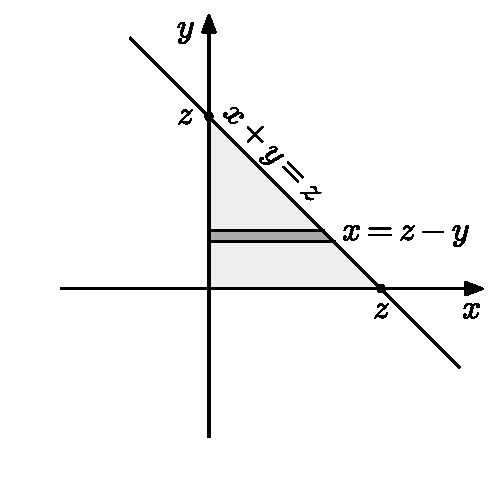
\includegraphics[width=\textwidth]{figuras/joint_distribution_region_rv_sum_positive.pdf}
  \end{minipage}\hfill
  \begin{minipage}[c]{0.56\textwidth}
    \caption{
       Región en el plano \(xy\) correspondiente al evento \(\{\x+\y\leq z\}\) cuando \(f_x(x)=0\) si \(x<0\) y \(f_y(y)=0\) si \(y<0\).
    } \label{fig:joint_distribution_region_rv_sum_positive}
  \end{minipage}
\end{figure}
Por lo tanto, la distribución de probabilidad es
\[
 F_z(z)=\int_{0}^{z}\int_{0}^{z-y}f_{xy}(x,\,y)\,dx\,dy.
\]
y la densidad de probabilidad se obtiene como
\begin{align*}
 f_z(z)=\frac{dF_z(z)}{dz}&=\frac{d}{dz}\left[\int_{0}^{z}\int_{0}^{z-y}f_{xy}(x,\,y)\,dx\,dy\right]\\
  &=\frac{d}{dz}\left[\int_{0}^{z}g(z,\,y)\,dy\right],
\end{align*}
donde se definió
\[
 g(z,\,y)\triangleq\int_{0}^{z-y}f_{xy}(x,\,y)\,dx.
\]
Aplicando la regla de integración de Leibnitz se tiene que
\[
 \frac{d}{dz}\left[\int_{0}^{z}g(z,\,y)\,dy\right]=g(z,\,z)+\int_{0}^{z}\frac{\partial g(z,\,x)}{\partial z}\,dx.
\]
Como 
\[
 g(z,\,z)=\int_{0}^{z-z}f_{xy}(x,\,y)\,dx=\int_{0}^{0}f_{xy}(x,\,y)\,dx=0,
\]
se obtiene que 
\begin{align*}
 f_z(z)&=\frac{d}{dz}\left[\int_{0}^{z}\int_{0}^{z-y}f_{xy}(x,\,y)\,dx\,dy\right]\\
   &=\int_{0}^{z}\left[\frac{\partial}{\partial z}\int_{0}^{z-y}f_{xy}(x,\,y)\,dx\right]\,dy\\
   &\overset{(a)}{=}\left\{\begin{array}{ll}
  \displaystyle\int_{0}^{z}f_{xy}(z-y,\,y)\,dy, & z > 0 \\
  \\
  0, & z\leq0
 \end{array} \right.
\end{align*}
donde en \((a)\) se diferenció aplicando la regla de Leibnitz y se tomó en cuenta que \(\z=\x+\y\geq0\) ya que \(\x\geq0\) y \(\y\geq0\).

\subsection{\texorpdfstring{Ejemplo: Densidad de probabilidad de \(\z=\x/\y\)}{}}

Sea \(\z=\x/\y\). Se quiere determinar \(f_z(z)\) en términos de \(f_{xy}(x,\,y)\). Se comenzará calculando
\[
 F_z(z)=P\{\x/\y\leq z\}.
\]
La inecuación \(x/y\leq z\) puede escribirse como \(\x\leq \y z\) si \(\y>0\) y como \(\x\geq\y z\) si \(\y<0\). Por lo tanto, el evento \(\{\x/\y\}\) tiene que ser condicionado al evento \(A=\{\y>0\}\) y su complemento \(\overline{A}\). Como \(A\cup\overline{A}=S\) y \(A\) y \(\overline{A}\) son mutuamente excluyentes, se cumple que
\begin{align*}
 P\{\x/\y\leq z\}&=P\{\x/\y\leq z\cap(A\cup\overline{A})\}\\
   &=P\{(\x/\y\leq z\cap A)\cup(\x/\y\leq z\cap\overline{A})\}\\
   &=P\{\x/\y\leq z,\,\y>0\}+P\{\x/\y\leq z,\,\y<0\}\\
   &=P\{\x\leq\y z,\,\y>0\}+P\{\x\leq\y z,\,\y<0\}
\end{align*}
\begin{figure}[!htb]
\begin{center}
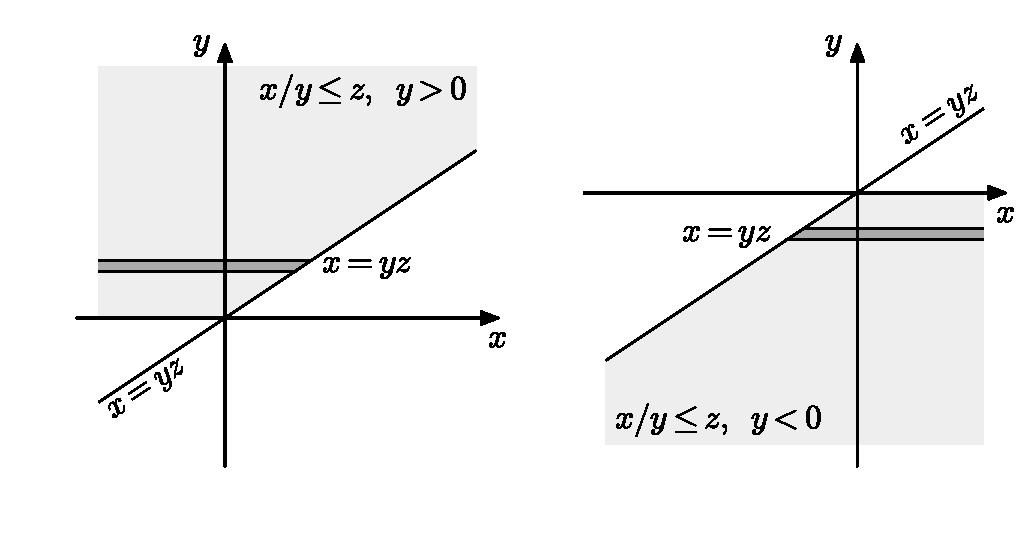
\includegraphics[width=0.75\columnwidth]{figuras/joint_distribution_region_rv_product.pdf}
\caption{\label{fig:joint_distribution_region_rv_product} Región de integración para determinar la densidad de probabilidad de \(\z=\x/\y\). A la derecha se muestra la región de integración de \(f_{xy}(x,\,y)\) para obtener \(P\{\x\leq\y z,\,\y>0\}\). La región se puede cubrir considerando una banda a lo largo del eje \(x\) desde \(x=-\infty\) a \(x=yz\) y desplazando la banda desde \(y=0\) hasta \(y=\infty\). A la izquierda se muestra la región de integración para obtener \(P\{\x\leq\y z,\,\y<0\}\). La región se puede cubrir considerando una banda a lo largo del eje \(x\) desde \(x=yz\) a \(x=\infty\) y desplazando la banda desde \(y=-\infty\) hasta \(y=0\).}
\end{center}
\end{figure}
En la figura \ref{fig:joint_distribution_region_rv_product} se muestra el área de integración correspondiente a cada sumando. Integrando sobre esas regiones, se obtiene que
\[
 F_z(z)=\int_{0}^{\infty}\int_{-\infty}^{yz}f_{xy}(x,\,y)\,dx\,dy+
   \int_{-\infty}^{0}\int_{yz}^{\infty}f_{xy}(x,\,y)\,dx\,dy.
\]
y diferenciando respecto a \(z\) empleando la regla de integración de Leibnitz, se obtiene la densidad de probabilidad,
\[
 f_z(z)=\int_{0}^{\infty}yf_{xy}(yz,\,y)\,dy+\int_{-\infty}^{0}-yf_{xy}(yz,\,y)\,dy,
\]
es decir,
\begin{equation}\label{eq:pdf_of_product_of_two_rv}
 f_z(z)=\int_{-\infty}^{\infty}|y|f_{xy}(yz,\,y)\,dy.
\end{equation}

En el caso en que \(\x\) e \(\y\) son variables aleatorias no negativas, la distribución de probabilidad queda
\[
 F_z(z)=\int_{0}^{\infty}\int_{0}^{yz}f_{xy}(x,\,y)\,dx\,dy
\]
y la densidad de probabilidad es
\[
 f_z(z)=\int_{0}^{\infty}yf_{xy}(yz,\,y)\,dy.
\]

\paragraph{Caso particular (Ejemplo 6-11)} Se considera el caso en que las variables aleatorias \(\x\) e \(\y\) son conjuntamente normales de media nula y densidad de probabilidad
\[
 f_{xy}(x,\,y)=\frac{1}{2\pi\sigma_1\sigma_2\sqrt{1-r^2}}\exp\left[-\frac{1}{2(1-r^2)}\left(\frac{x^2}{\sigma_1^2}-\frac{2rxy}{\sigma_1\sigma_2}+\frac{y^2}{\sigma_2^2}\right)\right],
\]
y se quiere calcular la distribución y densidad de probabilidad de \(\z=\x/\y\).

Como en este caso la densidad de probabilidad cumple que \(f_{xy}(-x,\,-y)=f_{xy}(x,\,y)\), la ecuación \ref{eq:pdf_of_product_of_two_rv} queda
\begin{equation}\label{eq:normal_rv_quotient_fz_tmp}
 f_z(z)=\int_{-\infty}^{\infty}|y|f_{xy}(yz,\,y)\,dy=f_z(z)=2\int_{0}^{\infty}yf_{xy}(yz,\,y)\,dy.
\end{equation}
El integrando contiene el término \(f_{xy}(yz,\,y)\), es decir, la densidad de probabilidad evaluada en \(x=yz\), y es
\begin{align}\label{eq:normal_rv_quotient_fxy}
 f_{xy}(yz,\,y)&=\frac{1}{2\pi\sigma_1\sigma_2\sqrt{1-r^2}}\exp\left[-\frac{1}{2(1-r^2)}\left(\frac{y^2z^2}{\sigma_1^2}-\frac{2ry^2z}{\sigma_1\sigma_2}+\frac{y^2}{\sigma_2^2}\right)\right]\nonumber\\
   &=\frac{1}{2\pi\sigma_1\sigma_2\sqrt{1-r^2}}\exp\left[-\frac{y^2}{2(1-r^2)}\left(\frac{z^2}{\sigma_1^2}-\frac{2rz}{\sigma_1\sigma_2}+\frac{1}{\sigma_2^2}\right)\right]\nonumber\\
   &=\frac{1}{2\pi\sigma_1\sigma_2\sqrt{1-r^2}}\exp\left(-\frac{y^2}{2\sigma_0^2}\right),
\end{align}
donde se definió
\[
 \sigma_0^2\triangleq\dfrac{1-r^2}{\dfrac{z^2}{\sigma_1^2}-\dfrac{2rz}{\sigma_1\sigma_2}+\dfrac{1}{\sigma_2^2}}.
\]
Notando que 
\[
 \left(\frac{z}{\sigma_1}-\frac{r}{\sigma_2}\right)^2=\frac{z^2}{\sigma_1^2}-\frac{2rz}{\sigma_1\sigma_2}+\frac{r^2}{\sigma_2^2},
\]
el denominador de \(\sigma_0^2\) se puede expresar como
\[
 \frac{z^2}{\sigma_1^2}-\frac{2rz}{\sigma_1\sigma_2}+\frac{1}{\sigma_2^2}=\left(\frac{z}{\sigma_1}-\frac{r}{\sigma_2}\right)^2+\frac{1}{\sigma^2_2}-\frac{r^2}{\sigma^2_2},
\]
por lo que
\begin{equation}\label{eq:normal_rv_quotient_sigma_0}
 \sigma_0^2=\dfrac{1-r^2}{\left(\dfrac{z}{\sigma_1}-\dfrac{r}{\sigma_2}\right)^2+\dfrac{1-r^2}{\sigma^2_2}}
   =\dfrac{\sigma_1^2\sigma_2^2\left(1-r^2\right)}{\sigma_2^2\left(z-\dfrac{\sigma_1}{\sigma_2}r\right)^2+\sigma_1^2(1-r^2)},
\end{equation}
donde en la segunda igualdad se multiplicó el numerador y el denominador entre \(\sigma_1^2\sigma_2^2\).
A partir de las ecuaciones \ref{eq:normal_rv_quotient_fz_tmp} y \ref{eq:normal_rv_quotient_fxy}, la densidad de probabilidad queda,
\begin{align*}
 f_z(z)&=2\int_{0}^{\infty}yf_{xy}(yz,\,y)\,dy\\
   &=\frac{1}{\pi\sigma_1\sigma_2\sqrt{1-r^2}}\int_{0}^{\infty}ye^{-y^2/2\sigma_0^2}\,dy\\
   &=\frac{1}{\pi\sigma_1\sigma_2\sqrt{1-r^2}}\left[-\sigma_0^2e^{-y^2/2\sigma_0^2}\bigg|_{0}^{\infty}\right]\\
   &=\frac{1}{\pi\sigma_1\sigma_2\sqrt{1-r^2}}\left[-\sigma_0^2\left(0-1\right)\right]\\
   &=\frac{\sigma_0^2}{\pi\sigma_1\sigma_2\sqrt{1-r^2}},
\end{align*}
y sustituyendo \(\sigma_0^2\) dado por la ecuación \ref{eq:normal_rv_quotient_sigma_0} se llega a que
\[
 f_z(z)=\dfrac{\sigma_1\sigma_2\sqrt{1-r^2}}{\pi\left[\sigma_2^2\left(z-\dfrac{\sigma_1}{\sigma_2}r\right)^2+\sigma_1^2(1-r^2)\right]}.
\]
Operando, se ve que \(f_z(z)\) se puede escribir como
\begin{align*}
 f_z(z)&\overset{(a)}{=}\dfrac{\sigma_1\sigma_2\sqrt{1-r^2}}{\pi\sigma_1^2(1-r^2)\left[\dfrac{\sigma_2^2\left(z-r\sigma_1/\sigma_2\right)^2}{\sigma_1^2(1-r^2)}+1\right]}\\
   &=\dfrac{1}{\pi\dfrac{\sigma_1}{\sigma_2}\sqrt{1-r^2}\left[\left(\dfrac{z-r\sigma_1/\sigma_2}{\dfrac{\sigma_1}{\sigma_2}\sqrt{1-r^2}}\right)^2+1\right]},
\end{align*}
donde en \((a)\) se multiplicó y dividió el denominador entre \(\sigma_1^2(1-r^2)\). Definiendo
\[
 \gamma\triangleq\frac{\sigma_1}{\sigma_2}\sqrt{1-r^2},\qquad z_0\triangleq r\sigma_1/\sigma_2,
\]
la densidad de probabilidad se puede expresar como
\begin{equation}\label{eq:cauchy_density_function}
 f_z(z)=\dfrac{1}{\pi\gamma\left[\left(\dfrac{z-z_0}{\gamma}\right)^2+1\right]},
\end{equation}
por lo que se concluye que \(\z=\x/\y\) es una variable aleatoria de Cauchy con centro \(z_0=r\sigma_1/\sigma_2\).

Integrando la ecuación \ref{eq:cauchy_density_function} entre \(-\infty\) a \(z\) se obtiene la distribución de probabilidad. Para hacerlo, se toma en cuenta que 
\begin{equation}\label{eq:normal_rv_arctan_derivative}
 \frac{d}{dx}(\arctan x)=\frac{1}{x^2+1}.
\end{equation}
Esta igualdad puede deducirse mediante diferenciación implícita de la siguiente forma. Se quiere calcular la derivada de la función
\[
 y(x)=\arctan x,\qquad-\frac{\pi}{2}<y<\frac{\pi}{2}.
\]
Se comienza despejando \(x\)
\begin{equation}\label{eq:normal_rv_arctan_derivative_aux}
 \tan y=x
\end{equation}
y luego se diferencia respecto a \(x\),
\[
 \frac{d}{dx}(\tan y)=\frac{d}{dx}x=1
\]
Desarrollando el lado izquierdo de la igualdad, se ve que
\[
 \frac{d}{dx}(\tan y)=\frac{d}{dx}\left(\frac{\sin y}{\cos y}\right)
 =\frac{\dfrac{dy}{dx}\cos^2y+\dfrac{dy}{dx}\sin^2y}{\cos^2y}
 =\dfrac{dy}{dx}\left(1+\tan^2y\right)
\]
y por lo tanto,
\[
 \dfrac{dy}{dx}\left(1+\tan^2y\right)=1.
\]
Despejando \(dy/dx\) se llega a que
\[
 \frac{dy}{dx}=\frac{1}{1+\tan^2y}=\frac{1}{1+x^2}.
\]
donde en la última igualdad se usó la ecuación \ref{eq:normal_rv_arctan_derivative_aux}. Se concluye que se verifica la ecuación \ref{eq:normal_rv_arctan_derivative}, a partir de la cual es fácil ver que
\[
 \frac{d}{dx}\left(\arctan \frac{x}{a}\right)=\frac{1}{a\left[\left(\dfrac{x}{a}\right)^2+1\right]}.
\]
De aquí se deduce que la primitiva de la densidad de probabilidad de la ecuación 
\ref{eq:cauchy_density_function} es
\[
 \frac{d}{dz}\left(\frac{1}{\pi}\arctan \frac{z-z_0}{\gamma}\right)
  =\dfrac{1}{\pi\gamma\left[\left(\dfrac{z-z_0}{\gamma}\right)^2+1\right]}=f_z(z)
\]
Por lo tanto, la distribución de probabilidad es
\begin{align*}
 F_z(z)&=\int_{-\infty}^zf_z(u)\,du\\
   &=\frac{1}{\pi}\left(\arctan \frac{u-z_0}{\gamma}\bigg|_{-\infty}^{z}\right)\\
   &\overset{(a)}{=}\frac{1}{\pi}\left(\arctan \frac{z-z_0}{\gamma}+\frac{\pi}{2}\right)\\
   &=\frac{1}{\pi}\arctan \frac{z-z_0}{\gamma}+\frac{1}{2},
\end{align*}
donde en \((a)\) se usó que \(\arctan u\to-\pi/2\) con \(u\to-\infty\).
Sustituyendo \(z_0\) y \(\gamma\) se obtiene que
\begin{align*}
 F_z(z)&=\frac{1}{\pi}\arctan \frac{z-r\sigma_1/\sigma_2}{\dfrac{\sigma_1}{\sigma_2}\sqrt{1-r^2}}+\frac{1}{2}\\
   &=\frac{1}{\pi}\arctan \frac{z\sigma_2-r\sigma_1}{\sigma_1\sqrt{1-r^2}}+\frac{1}{2}.
\end{align*}

\subsection{Estadísticos de orden}

Considérese una \(n\)-tupla de valores \(\x_1,\,\x_2,\dots,\,\x_n\). El subíndice \(k\) en \(\x_k\) puede indicar un orden temporal, pero usualmente no es significativo. Un ejemplo en donde el subíndice es significativo es en el caso en que la \(n\)-tupla forma parte de una serie temporal. La \(n\)-tupla puede ordenarse de forma creciente como
\[
 \x_{(1)}\leq\x_{(2)}\leq\dots\leq\x_{(n)},
\]
donde \(\x_{(1)}=\min(\x_1,\,\x_2,\dots,\,\x_n)\), \(\x_{(2)}\) es el segundo valor mas pequeño y así sucesivamente hasta \(\x_{(n)}=\max(\x_1,\,\x_2,\dots,\,\x_n)\). En el caso en que \(\x_1,\,\x_2,\dots,\,\x_n\) son variables aleatorias, la función \(\x_{(k)}\) que toma el valor \(x_{(k)}\) en cada posible secuencia \((x_1,\,x_2,\dots,\,x_n)\) se llama estadístico de orden \(k\)-ésimo. El conjunto \(\{\x_{(1)},\,\x_{(2)},\dots,\,\x_{(n)}\}\) representa los estadísticos de orden entre \(n\) variables aleatorias. En este contexto, 
\[
 \mathbf{R}=\x_{(n)}-\x_{(1)}
\]
representa el estadístico \emph{rango}. En el caso en que \(n=2\), se tienen los estadísticos \emph{máximo} y \emph{mínimo}.

\paragraph{\texorpdfstring{Ejemplo: Densidad de probabilidad de \(\z=\max(\x,\,\y)\)}{}}

Sea \(\z=\max(\x,\,\y)\). Se quiere determinar \(f_z(z)\). Como
\[
 \z=\max(\x,\,\y)=
 \left\{\begin{array}{ll}
  \x, & \x>\y \\
  \y, & \x\leq\y
 \end{array} \right.,
\]
la distribución de probabilidad es
\begin{align}\label{eq:joint_distribution_rv_max_aux}
 F_z(z)&=P\{\max(\x,\,\y)\leq z\}\nonumber\\
   &=P\{(\max(\x,\,\y)\leq z)\cap(\x>\y\cup\x\leq\y)\}\nonumber\\
   &=P\{(\max(\x,\,\y)\leq z\cap \x>\y)\cup(\max(\x,\,\y)\leq z\cap\x\leq\y)\}\nonumber\\
   &=P\{\x\leq z,\, \x>\y\}+P\{\y\leq z,\,\x\leq\y\},
\end{align}
ya que \(\{\x>\y\}\) y \(\{\x\leq\y\}\) son eventos mutuamente excluyentes y forman una partición del espacio muestral. En la figura \ref{fig:joint_distribution_region_rv_max} se muestran las regiones correspondientes a cada sumando de la ecuación \ref{eq:joint_distribution_rv_max_aux}, así como la unión de las regiones.
\begin{figure}[!htb]
\begin{center}
 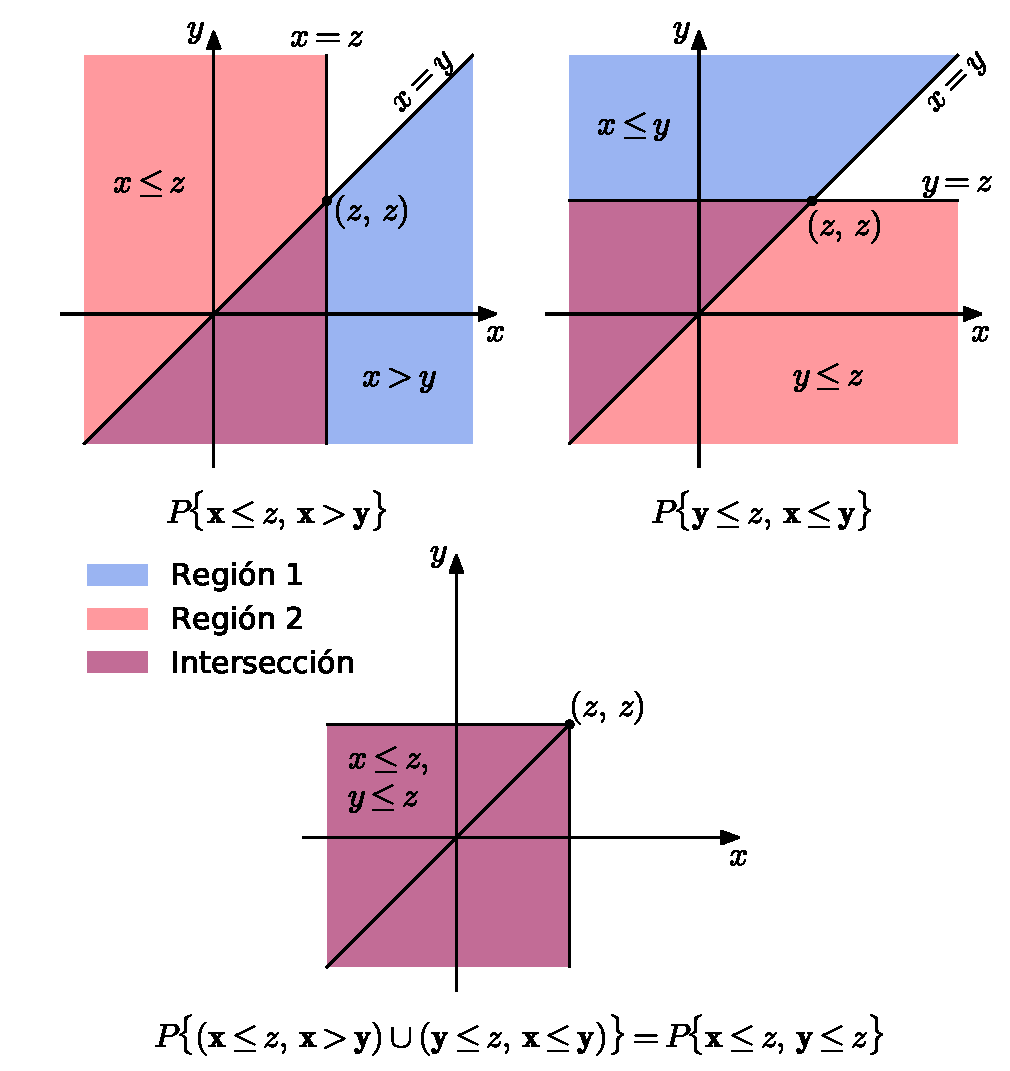
\includegraphics[width=0.7\columnwidth]{figuras/joint_distribution_region_rv_max.pdf}
\caption{\label{fig:joint_distribution_region_rv_max} Región del plano correspondiente a \(F_z(z)=P\{\max(\x,\,\y)\leq z\}\).}
\end{center}
\end{figure}
De la figura, se obtiene que
\begin{equation}\label{eq:joint_distribution_rv_max}
 F_z(z)=P\{\x\leq z,\, \y\leq z\}=F_{xy}(z,\,z).
\end{equation}
En el caso en que \(\x\) e \(\y\) son variables aleatorias independientes, la distribución queda
\[
 F_z(z)=F_x(z)F_y(z),
\]
y diferenciando respecto a \(z\) se obtiene la densidad de probabilidad, que es
\[
 f_z(z)=F_x(z)f_y(z)+f_x(z)F_y(z).
\]

\paragraph{\texorpdfstring{Ejemplo: Densidad de probabilidad de \(\w=\min(\x,\,\y)\)}{}}

Considérese ahora el caso en que \(\z=\min(\x,\,\y)\). Se quiere determinar \(f_z(z)\). Como
\[
 \w=\min(\x,\,\y)=
 \left\{\begin{array}{ll}
  \y, & \x>\y \\
  \x, & \x\leq\y
 \end{array} \right.,
\]
realizando un razonamiento análogo al caso anterior, se tiene que
\begin{align}\label{eq:joint_distribution_rv_min_aux}
 F_w(w)&=P\{\min(\x,\,\y)\leq w\}\nonumber\\
   &=P\{\y\leq w,\, \x>\y\}+P\{\x\leq w,\,\x\leq\y\}.
\end{align}
En la figura \ref{fig:joint_distribution_region_rv_min} se muestran las regiones del plano correspondientes a las desigualdades de la ecuación \ref{eq:joint_distribution_rv_min_aux}, y también la unión de dichas regiones.
\begin{figure}[!htb]
\begin{center}
 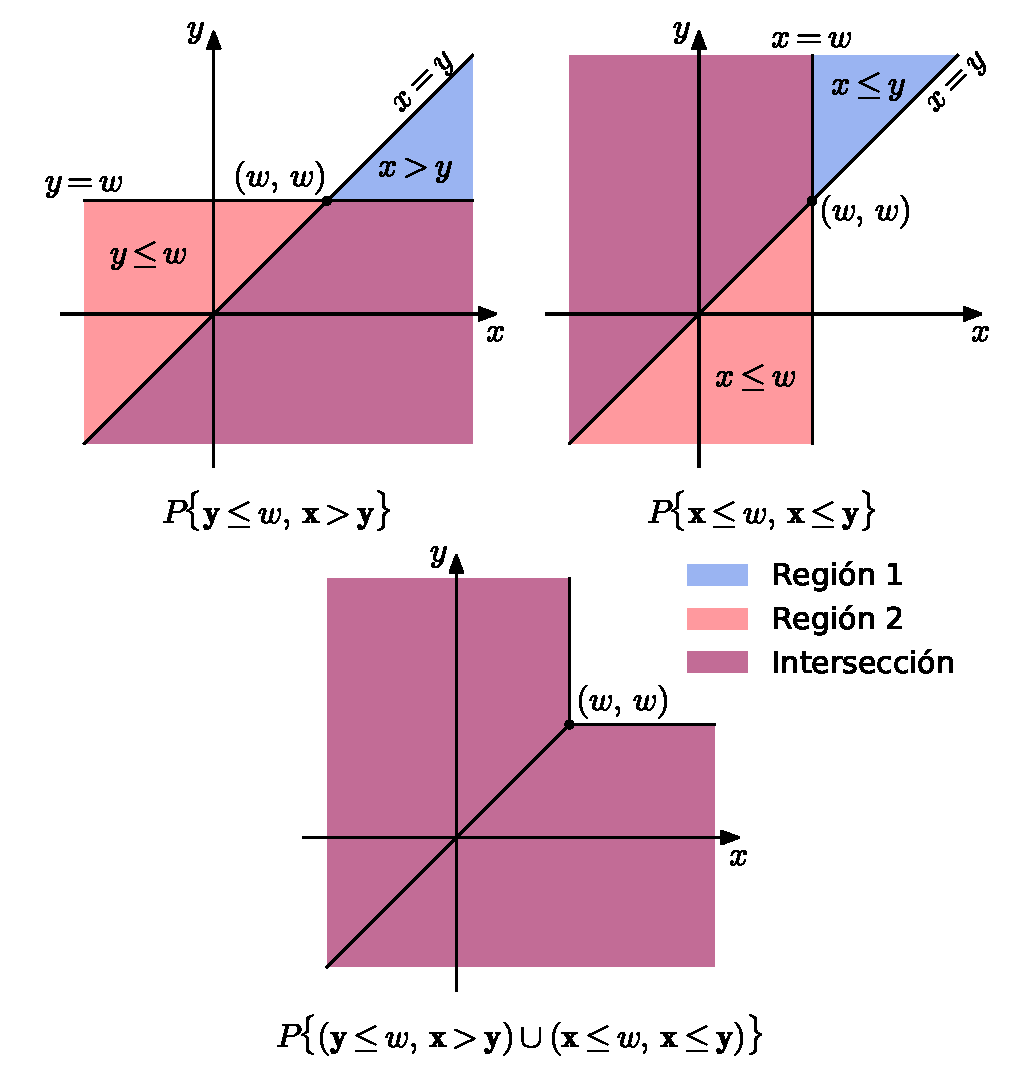
\includegraphics[width=0.7\columnwidth]{figuras/joint_distribution_region_rv_min.pdf}
\caption{\label{fig:joint_distribution_region_rv_min} Región del plano correspondiente a \(F_z(z)=P\{\min(\x,\,\y)\leq z\}\).}
\end{center}
\end{figure}
A partir de la figura, se tiene que
\[
 F_w(w)=1-P\{\x>w,\y>w\},
\]
ya que la probabilidad conjunta del todo el plano es \(F(\infty,\,\infty)=P\{x\leq\infty,\,y\leq\infty\}=1\). Además, se ve que
\begin{align*}
 P\{\x>w,\y>w\}&=P\{w<\x\leq \infty,\,w<\y\leq \infty\}\\
   &\overset{(a)}{=}F(\infty,\,\infty)-F(w,\,\infty)-F(\infty,\,w)+F(w,\,w)\\
   &\overset{(b)}{=}1-F_x(w)-F_y(w)+F_{xy}(w,\,w),
\end{align*}
donde en \((a)\) se usó la ecuación \ref{eq:joint_distribution_rectangular_region} y en \((b)\) las estadísticas marginales. Sustituyendo este resultado en la ecuación anterior, se obtiene que
\[
 F_w(w)=1-[1-F_x(w)-F_y(w)+F_{xy}(w,\,w)],
\]
concluyendo que
\begin{equation}\label{eq:joint_distribution_rv_min}
 F_w(w)=F_x(w)+F_y(w)-F_{xy}(w,\,w).
\end{equation}

\section{Dos funciones de dos variables aleatorias}\label{sec:two_funcions_of_two_rv}

Se considera ahora una generalización del caso de la sección anterior. Sean \(\x\) e \(\y\) variables aleatorias con densidad de probabilidad conjunta \(f_{xy}(x,\,y)\). Dadas dos funciones \(g(x,\,y)\) y \(h(x,\,y)\), se definen dos nuevas variables aleatorias
\begin{align*}
 \z&=g(\x,\,\y)\\
 \w&=h(\x,\,\y),
\end{align*}
y se quiere determinar la densidad de probabilidad conjunta \(f_{zw}(z,\,w)\). Luego, los marginales \(f_z(z)\) y \(f_w(w)\) pueden obtenerse integrando \(f_{zw}(z,\,w)\).

De forma análoga al caso de una función de dos variables aleatorias dado en la ecuación \ref{eq:pdf_of_funcion_of_two_rv}, la distribución de probabilidad es
\begin{align}\label{eq:pdf_of_two_funcion_of_two_rv}
 F_{zw}(z,\,w)&=P\{\z\leq z,\,\w\leq w\}\nonumber\\
    &=P\{g(\x,\,\y)\leq z,\,h(\x,\,\y)\leq w\}\nonumber\\
    &=P\{(\x,\,\y)\in D_{z,\,w}\}\nonumber\\
    &=\iint_{(x,\,y)\in D_{z,\,w}}f_{xy}(x,\,y)\,dx\,dy,
\end{align}
donde \(D_{z,\,w}\) es la región en el plano \(xy\) donde las inecuaciones \(g(x,\,y)\leq z\) y \(h(x,\,y)\leq w\) se cumplen simultáneamente. La densidad de probabilidad conjunta \(f_{zw}(z,\,w)\) puede obtenerse a partir de las derivadas de la distribución de probabilidad \(F_{zw}(z,\,w)\) (ecuación  \ref{eq:joint_density_definition}), pero como se verá mas adelante, también puede obtenerse directamente de \(f_{xy}(x,\,y)\).

\paragraph{Ejemplo} Sean \(\x\) e \(\y\) variables aleatorias independientes de distribución uniforme en el intervalo \((0,\,\theta)\). Se definen las variables aleatorias \(\z=\max(\x,\,\y)\) y \(\w=\min(\x,\,\y)\). Se quiere determinar \(f_{zw}(z,\,w)\).

Se comenzará calculando la distribución de probabilidad \(F_{zw}(z,\,w)\). La densidad de probabilidad \(f_{zw}(z,\,w)\) se obtiene diferenciando la distribución. Por definición,
\[
 F_{zw}(z,\,w)=P\{\z\leq z,\,\w\leq w\}=P\{\max(\x,\,\y)\leq z,\,\min(\x,\,\y)\leq w\}.
\]
Como \(\x\) e \(\y\) varían en el intervalo \((0,\,\theta)\), \(\z=\max(\x,\,\y)\) y \(\w=\min(\x,\,\y)\) varían en el mismo intervalo. Por lo tanto,
\[
 F_{zw}(z,\,w)=0, \qquad\textrm{si }z<0\quad\textrm{o}\quad w<0.
\]
La región de integración \(D_{z,\,w}\) en la ecuación \ref{eq:pdf_of_two_funcion_of_two_rv} se trata de la intersección de las regiones de integración de las figuras \ref{fig:joint_distribution_region_rv_max} y \ref{fig:joint_distribution_region_rv_min}, por lo que hay que diferenciar los casos \(w\geq z\) y \(w<z\), ya que dan lugar a regiones distintas, como se muestra en la figura \ref{fig:joint_distribution_region_rv_min_max}.
\begin{figure}[!htb]
\begin{center}
 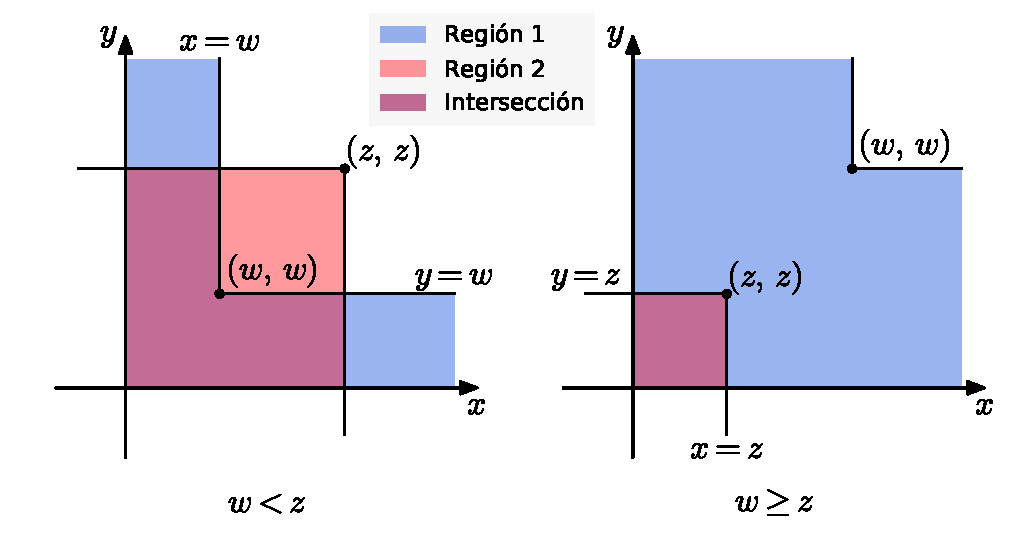
\includegraphics[width=0.70\columnwidth]{figuras/joint_distribution_region_rv_min_max.pdf}
\caption{\label{fig:joint_distribution_region_rv_min_max} Regiones del plano correspondientes a \(F_z(z,\,w)=P\{\max(\x,\,\y)\leq z,\,\min(\x,\,\y)\leq w\}\).}
\end{center}
\end{figure}

En el caso en que \(w<z\), observando la región intersección en la figura \ref{fig:joint_distribution_region_rv_min_max}, se deduce que
\[
 F_{zw}(z,\,w)=F_{xy}(z,\,w)+F_{xy}(w,\,z)-F_{xy}(w,\,w),\qquad 0\leq w< z<\theta,
\]
ya que \(F_{xy}(z,\,w)\) es el rectángulo horizontal de vértices \((z,\,w)\) y \((0,\,0)\) en las diagonales, \(F_{xy}(z,\,w)\) es el rectángulo vertical de vértices \((w,\,z)\) y \((0,\,0)\) en las diagonales, y como estas regiones se solapan, se está considerando dos veces el cuadrado de vértices \((w,\,w)\) y \((0,\,0)\) en las diagonales, por lo que hay que restar \(F_{xy}(w,\,w)\). En el caso en que \(w\geq z\), de la figura \ref{fig:joint_distribution_region_rv_min_max} se obtiene que
\[
 F_{zw}(z,\,w)=F_{xy}(z,\,z),\qquad 0\leq z\leq w<\theta.
\]
Además, en el caso en que \(w>\theta\) se cumple que
\begin{align*}
  F_{zw}(z,\,w)&=P\{\z\leq z,\,\w\leq w\}\\
   &=P\{(\z\leq z)\cap(\w\leq w)\}\\
   &\overset{(a)}{=}P\{(\z\leq z)\cap S\}\\
   &\overset{(b)}{=}P\{\z\leq z\}\\
   &=F_z(z),
\end{align*}
donde en \((a)\) se tuvo en cuenta que como \(w>\theta\) y \(\w\) varía en el intervalo \((0,\,\theta)\), se cumple que
\begin{align*}
 \{\w\leq w\}=\{(\w<\theta)\cup(\theta\leq\w\leq w)\} = \{(\w<\theta)\cup\emptyset\} = \{\w<\theta\} = S
\end{align*}
es decir, el evento \(\{\w\leq w\}\) es todo el espacio muestral \(S\), y en \((b)\) se consideró que si \(A\)  es un evento arbitrario, se cumple que \(A\cap S=A\). De este razonamiento se concluye que
\[
\def\arraystretch{1.2}
 \begin{array}{lll}
  F_{zw}(z,\,w)=F_z(z)\overset{(a)}{=}F_{xy}(z,\,z), & & 0\leq z<\theta\leq w.\\
  F_{zw}(z,\,w)=F_w(w)\overset{(b)}{=}F_x(w)+F_y(w)-F_{xy}(w,\,w), & & 0\leq w<\theta\leq z\\
  F_{zw}(z,\,w)=1, & & z\geq\theta\quad\textrm{y}\quad w\geq\theta,
 \end{array}
\]
donde en \((a)\) y en \((b)\) se usaron los resultados de las ecuaciones \ref{eq:joint_distribution_rv_max} y \ref{eq:joint_distribution_rv_min} respectivamente.
Juntando estos resultados se llega a que
\begin{equation}\label{eq:joint_distribution_rv_min_max_aux}
 \def\arraystretch{1.8}
 F_{zw}(z,\,w)=\left\{\begin{array}{ll}
  0, & z<0\quad\textrm{o}\quad w<0 \\
  F_{xy}(z,\,w)+F_{xy}(w,\,z)-F_{xy}(w,\,w),& 0\leq w<z<\theta\\
  F_{xy}(z,\,z),& 0\leq z\leq w<\theta\\
  F_{xy}(z,\,z), & 0\leq z<\theta\leq w\\
  F_x(w)+F_y(w)-F_{xy}(w,\,w), & 0\leq w<\theta\leq z\\
  1, & z\geq\theta\quad\textrm{y}\quad z\geq\theta.
 \end{array} \right.
\end{equation}
Por otro lado, como \(\x\sim U(0,\,\theta)\) e \(\y\sim U(0,\,\theta)\), su distribución de probabilidad es
\[
 F_x(x)=F_y(x)=\left\{\begin{array}{ll}
  0, & x<0 \\
  \dfrac{x}{\theta}, & 0\leq x<\theta\\
  1, & x\geq 0
 \end{array} \right.
\]
y como además son independientes, 
\[
\def\arraystretch{1.8}
 F_{xy}(x,\,y)=F_x(x)F_y(y)=\left\{\begin{array}{ll}
  0, & x<0\quad\textrm{o}\quad y<0 \\
  \dfrac{x}{\theta}\cdot\dfrac{y}{\theta}=\dfrac{xy}{\theta^2}, & 0\leq x<\theta\quad\textrm{y}\quad 0\leq y<\theta\\
  \dfrac{x}{\theta}, & 0\leq x<\theta\leq y\\
  \dfrac{y}{\theta}, & 0\leq y<\theta\leq x\\
  1, & x\geq\theta\quad\textrm{y}\quad y\geq\theta.
 \end{array} \right.
\]
Finalmente, sustituyendo estos resultados en la ecuación \ref{eq:joint_distribution_rv_min_max_aux} se llega a que
\begin{equation}\label{eq:joint_distribution_rv_min_max}
 \def\arraystretch{1.8}
 F_{zw}(z,\,w)=\left\{\begin{array}{ll}
  0, & z<0\quad\textrm{o}\quad w<0 \\
  \dfrac{zw}{\theta^2}+\dfrac{zw}{\theta^2}-\dfrac{w^2}{\theta^2}=\dfrac{2zw-w^2}{\theta^2},& 0\leq w<z<\theta\\
  \dfrac{z^2}{\theta^2},& 0\leq z\leq w<\theta\\
  \dfrac{z^2}{\theta^2}, & 0\leq z<\theta\leq w\\
  \dfrac{w}{\theta}+\dfrac{w}{\theta}-\dfrac{w^2}{\theta^2}=\dfrac{2\theta w-w^2}{\theta^2}, & 0\leq w<\theta\leq z\\
  1, & z\geq\theta\quad\textrm{y}\quad z\geq\theta.
 \end{array} \right.
\end{equation}
En la figura \ref{fig:joint_distribution_region_rv_min_max_surface_colormap_v4} se muestra la distribución de probabilidad \(F_{zw}(z,\,w)\).
\begin{figure}[!htb]
\begin{center}
 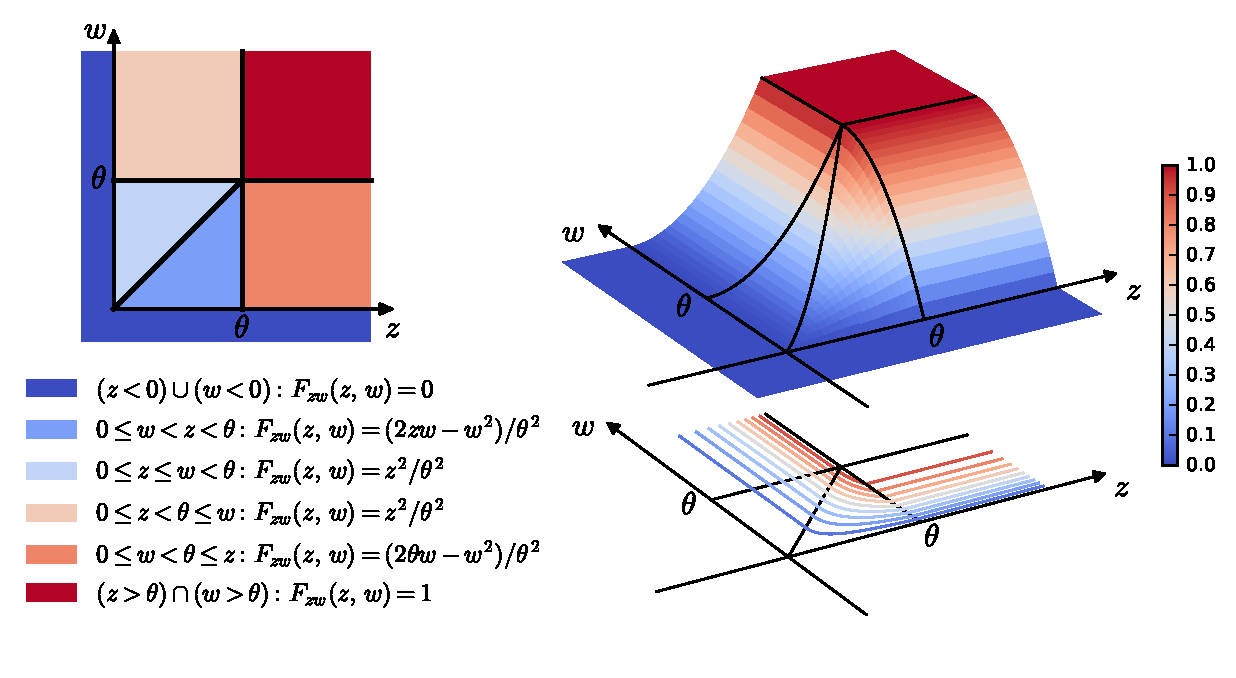
\includegraphics[width=1\columnwidth]{figuras/joint_distribution_region_rv_min_max_surface_colormap_v4.pdf}
\caption{\label{fig:joint_distribution_region_rv_min_max_surface_colormap_v4} Distribución de probabilidad \(F_z(z,\,w)=P\{\max(\x,\,\y)\leq z,\,\min(\x,\,\y)\leq w\}\). A la izquierda se muestra el valor que toma la función en las distintas regiones del plano. A la derecha se muestra la superficie \(F_{zw}(z,\,w)\) y las curvas de nivel en función de \(z\) y \(w\).}
\end{center}
\end{figure}

La densidad de probabilidad puede calcularse como
\[
 f_{zw}(z,\,w)=\frac{\partial^2F_{zw}(z,\,w)}{\partial z\partial w},
\]
lo que resulta en
\[
 f_{zw}(z,\,w)=\left\{\begin{array}{ll}
  \dfrac{2}{\theta^2},& 0\leq w<z<\theta\\
  0, \quad\textrm{en otro caso.}
 \end{array} \right.
\]
la cual se muestra en la figura \ref{fig:joint_density_function_rv_min_max_surface_v2}.
\begin{figure}[!htb]
  \begin{minipage}[c]{0.5\textwidth}
    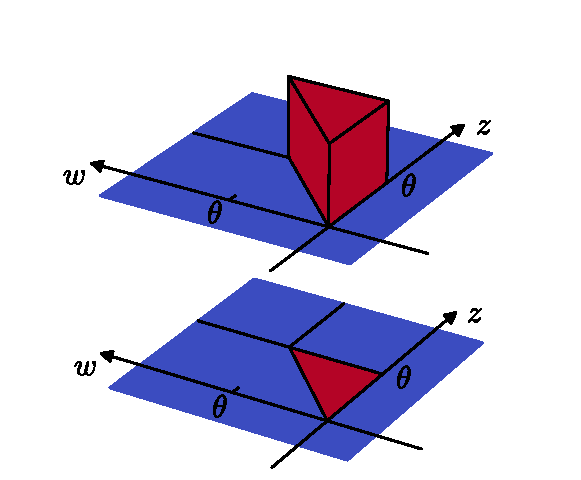
\includegraphics[width=\textwidth]{figuras/joint_density_function_rv_min_max_surface_v2.pdf}
  \end{minipage}\hfill
  \begin{minipage}[c]{0.42\textwidth}
    \caption{
       Densidad de probabilidad \(f_{zw}(z,\,w)\) de la variables aleatorias \(\z=\max(\x,\,\y)\) y \(\w=\min(\x,\,\y)\). \(f_{zw}(z,\,w)\) toma el valor constante \(2/\theta^2\) en la región triangular \(0\leq w<z<\theta\)  y 0 en el resto del plano \(zw\).
    } \label{fig:joint_density_function_rv_min_max_surface_v2}
  \end{minipage}
\end{figure}

Integrando la densidad de probabilidad \(f_{zw}(z,\,w)\) como indica la ecuación \ref{eq:pdf_of_two_funcion_of_two_rv}, puede obtenerse la distribución de probabilidad \(F_{zw}(z,\,w)\),
\[
 F_{zw}(z,\,w)=\int_{-\infty}^{z}\int_{-\infty}^{w}f_{zw}(z,\,w)\,dw\,dz,
\]
Esto consiste en calcular el volumen de \(f_{zw}(z,\,w)\) en el cuadrante determinado por las semirectas \((-\infty,\,z)\) y \((-\infty,\,w)\) para todo valor de \((z,\,w)\). Como en este ejemplo \(f_{zw}(z,\,w)\) es una función sencilla, constante en una región triangular, el cálculo puede realizarse de forma geométrica, teniendo en cuenta que el volumen cambia según la región del plano donde se encuentren \(z\) y \(w\), como se muestra en la figura \ref{fig:joint_density_function_rv_min_max_integration}.
\begin{figure}[!htb]
\begin{center}
 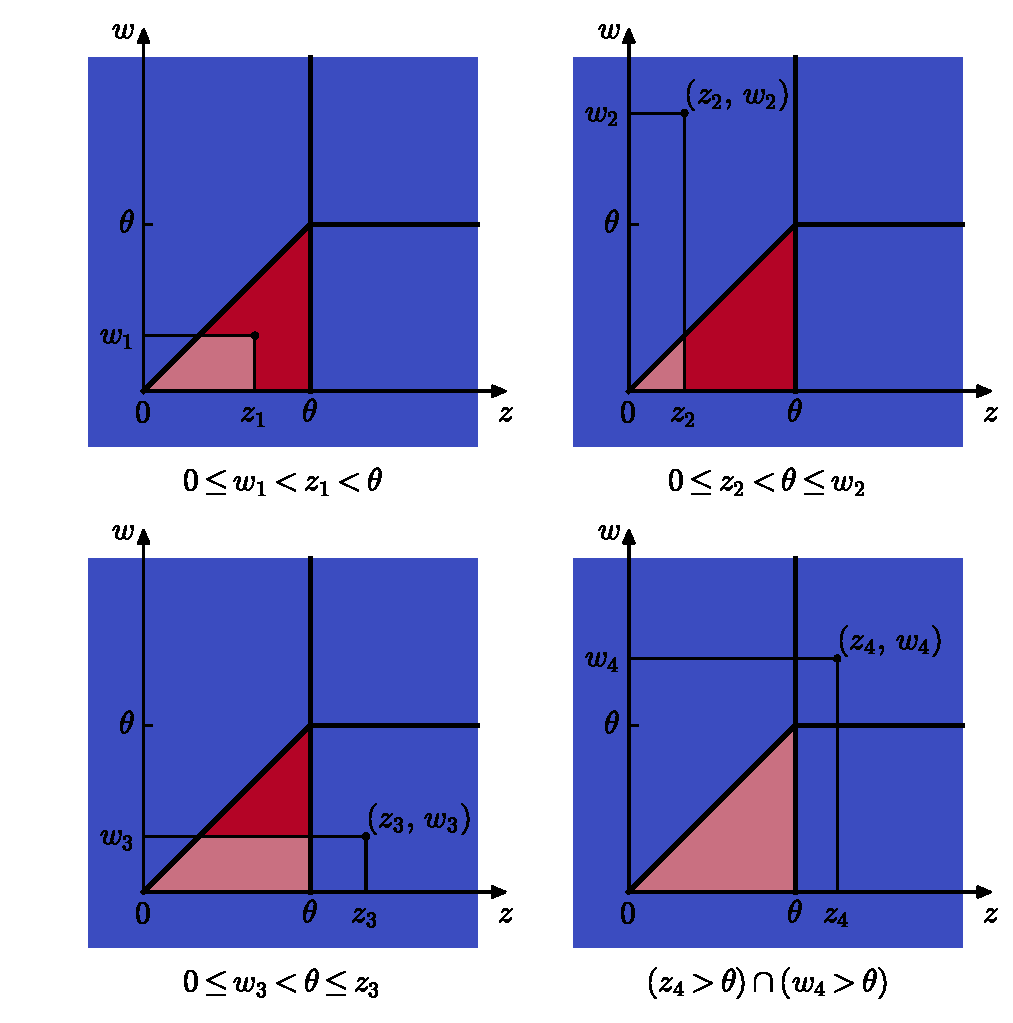
\includegraphics[width=0.85\columnwidth]{figuras/joint_density_function_rv_min_max_integration.pdf}
\caption{\label{fig:joint_density_function_rv_min_max_integration} Cálculo de \(F_{zw}(z,\,w)\) a partir de la integración de \(f_{zw}(z,\,w)\). En la figura se muestra el área de la base para el cálculo del volumen abarcado por \(f_{zw}(z,\,w)\) según la región del plano donde se encuentren \(z\) y \(w\).}
\end{center}
\end{figure}
Para hacerlo, se observa que:
\begin{itemize}
 \item si \(0\leq w<z<\theta\) como \(z_1\) y \(w_1\) en la figura \ref{fig:joint_density_function_rv_min_max_integration}, el área de la base es
 \[
  \textrm{Área}=\frac{w^2}{2}+(z-w)w=zw-\frac{w^2}{2},
 \]
y la altura es \(f_{zw}(z,\,w)=2/\theta^2\), por lo que el volumen es
\[
 F_{zw}(z,\,w)=\left(zw-\frac{w^2}{2}\right)\frac{2}{\theta^2}=\frac{2zw-w^2}{\theta^2}.
\]
\item si \(0\leq z<\theta\) y \(z<w\) como \(z_2\) y \(w_2\) en la figura \ref{fig:joint_density_function_rv_min_max_integration}, se tiene que
\[
 F_{zw}(z,\,w)=\frac{z^2}{2}\cdot\frac{2}{\theta^2}=\frac{z^2}{\theta^2}.
\]
\item si \(0\leq w<\theta\leq z\) como \(z_3\) y \(w_3\) en la figura \ref{fig:joint_density_function_rv_min_max_integration}, se tiene que
\[
 F_{zw}(z,\,w)=\left((\theta-w)w+\frac{w^2}{2}\right)\frac{2}{\theta^2}=\frac{2\theta w-w^2}{\theta^2}.
\]
\item si \(z>\theta\) y \(w>\theta\) como \(z_4\) y \(w_4\) en la figura \ref{fig:joint_density_function_rv_min_max_integration}, se tiene que
\[
 F_{zw}(z,\,w)=\frac{\theta^2}{2}\cdot\frac{2}{\theta^2}=1.
\]
\end{itemize}
Este resultado coincide con el de la ecuación \ref{eq:joint_distribution_rv_min_max}.

\subsection{Densidad de probabilidad conjunta}

Sean \(g(x,\,y)\) y \(h(x,\,y)\) dos funciones continuas y diferenciables y dos variables aleatorias \(\x\) e \(\y\). Se definen las variables aleatorias \(\z\) y \(\w\) como
\begin{align*}
 \z&=g(\x,\,\y)\\
 \w&=h(\x,\,\y),
\end{align*}
Se puede demostrar que las densidades de probabilidad \(f_{xy}(x,\,y)\) y \(f_{zw}(z,\,w)\) se vinculan como
\begin{equation}\label{eq:joint_density_two_funcions_two_rv}
 f_{zw}(z,\,w)=\sum_{i}|J(z,\,w)|f_{xy}(x_i,\,y_i)=\sum_{i}\frac{1}{|J(x_i,\,y_i)|}f_{xy}(x_i,\,y_i),
\end{equation}
donde \((x_i,\,y_i)\) son todas las soluciones del sistema de ecuaciones
\begin{equation}\label{eq:joint_density_two_rv_transformation}
 g(x,\,y)=z,\qquad h(x,\,y)=w
\end{equation}
para un punto dado \((z,\,w)\), es decir, \((x_1,\,y_1),\,(x_2,\,y_2),\dots,\,(x_n,\,y_n)\) son todos los puntos tal que
\[
 g(x_i,\,y_i)=z,\qquad h(x_i,\,y_i)=w.
\]
Equivalentemente, si \(g_1\) y \(h_1\) es la transformación inversa a \ref{eq:joint_density_two_rv_transformation}, se cumple que
\[
 x_i=g_1(z,\,w),\qquad y_i=h_1(z,\,w).
\]
Además, \(|J(z,\,w)|\) y \(|J(x_i,\,y_i)|\) son el valor absoluto del determinante de la matriz Jacobiana de la transformación inversa y directa respectivamente, es decir,
\begingroup
\renewcommand*{\arraystretch}{2.2}
\[
 J(z,\,w)=
 \begin{vmatrix}
    \dfrac{\partial g_1}{\partial z} & \dfrac{\partial g_1}{\partial w} \\
    \dfrac{\partial h_1}{\partial z} & \dfrac{\partial h_1}{\partial w}
\end{vmatrix}
\qquad\qquad
J(x_i,\,y_i)=
 \begin{vmatrix}
    \dfrac{\partial g}{\partial x} & \dfrac{\partial g}{\partial y} \\
    \dfrac{\partial h}{\partial x} & \dfrac{\partial h}{\partial y}
\end{vmatrix}_{x=x_1,\,y=y_i}.
\]
\endgroup
Como la matriz inversa de la matriz Jacobiana de una transformación invertible es la matriz Jacobiana de la transformación inversa, se cumple que
\[
 |J(z,\,w)|=\frac{1}{|J(x_i,\,y_i)|}.
\]

\paragraph{Transformación lineal}
Sean
\[
 \z=a\x+b\y,\qquad \y=c\x+d\y.
\]
Se quiere calcular \(f_{zw}(z,\,w)\). Se considera el sistema de ecuaciones
\[
\arraycolsep=1.4pt
 \left\{
 \begin{array}{lllll}
  ax&+&by&=&z\\
  cx&+&dy&=&w
 \end{array} \right..
\]
La solución del sistema es (regla de Cramer)
\[
 x=\frac{\Delta x}{\Delta},\qquad y=\frac{\Delta y}{\Delta}
\]
con
\[
\Delta=
\begin{vmatrix}
  a & b \\
  c & d
\end{vmatrix}
=ad-bc,
\quad
\Delta x=
\begin{vmatrix}
  z & b \\
  w & d
\end{vmatrix}
=zd-bw,
\quad
\Delta y=
\begin{vmatrix}
  a & z \\
  c & w
\end{vmatrix}
=aw-zc
\]
y el sistema tiene una única solución si \(\Delta=ad-bc\neq0\). En ese caso, se obtiene que
\[
 x=\frac{dz-bw}{ad-bc}=Az+Bw,\qquad y=\frac{-cz+aw}{ad-bc}=Cz+Dw.
\]
Como
\[
 g(x,\,y)=ax+by,\qquad h(x,\,y)=cx+dy,
\]
\(J(x,\,y)=ad-bc\),
por lo que sustituyendo estos resultados en la ecuación \ref{eq:joint_density_two_funcions_two_rv} se llega a que
\begin{equation}\label{eq:two_rv_linear_transformation}
 f_{zw}(z,\,w)=\frac{1}{|ad-bc|}f_{xy}(Az+Bw,\,Cz+Dw).
\end{equation}

\paragraph{Ejemplo: variables aleatorias conjuntamente normales}

Sean las variables aleatorias \(\x\) e \(\y\) conjuntamente normales con densidad \(N(\eta_x,\,\eta_y,\,\sigma_x^2,\,\sigma_y^2,\,\rho)\). Se definen las variables aleatorias \(\z\) y \(\w\) como la siguiente transformación lineal de \(\x\) e \(\y\),
\[
 \z=a\x+b\y,\qquad \w=c\x+d\y.
\]
La densidad de probabilidad conjunta \(f_{zw}(z,\,w)\) se obtiene a partir de la ecuación \ref{eq:two_rv_linear_transformation} con \(f_{xy}(x,\,y)\) dada por las ecuaciones \ref{eq:joint_normal_pdf1} y \ref{eq:joint_normal_pdf2}. Operando, puede verse que \(f_{zw}(z,\,w)\) es una exponencial con exponente cuadrático en \(z\) y \(w\) de la misma forma de \(f_{xy}(x,\,y)\). Se concluye que \(\z\) y \(\w\) también son conjuntamente normales con densidad conjunta \(N(\eta_z,\,\eta_w,\,\sigma_z^2,\,\sigma_w^2,\,\rho_{zw})\) con
\begin{equation}\label{eq:jointly_normal_linear_transformation}
 \begin{aligned}
 \eta_z&=a\eta_x+b\eta_y\\
 \eta_w&=c\eta_x+d\eta_y\\
 \sigma_z^2&=a^2\sigma_x^2+2ab\rho\sigma_x\sigma_y+b^2\sigma_y^2\\
 \sigma_w^2&=c^2\sigma_x^2+2cd\rho\sigma_x\sigma_y+d^2\sigma_y^2\\
 \rho_{zw}&=\dfrac{ac\sigma_x^2+(ad+bc)\rho\sigma_x\sigma_y+bd\sigma_y^2}{\sigma_z\sigma_w}.
\end{aligned}
\end{equation}
En general, cualquier combinación lineal de dos variables aleatorias conjuntamente normales es normal. La deducción de estos resultados es tediosa, por lo que se omite aquí pero se hará mas adelante usando la función característica.


\paragraph{Ejemplo 6-22} Sean \(\x\) e \(\y\) dos variables aleatorias independientes, de distribución gaussiana, con media nula y varianza común \(\sigma^2\). Se definen las variables aleatorias
\begin{equation}\label{eq:magnitude_and_phase_rv}
 \mathbf{r}=\sqrt{\x^2+\y^2}, \qquad\bm{\theta}=\tan^{-1}(\y/\x),
\end{equation}
con \(|\theta|<\pi\), y se quiere calcular su densidad de probabilidad conjunta.

Como las variables aleatorias \(\x\) e \(\y\) son independientes, su densidad de probabilidad conjunta es
\begin{align*}
 f_{xy}(x,\,y)&=f_x(x)f_y(y)\\
   &=\left(\frac{1}{\sigma\sqrt{2\pi}}e^{-x^2/2\sigma^2}\right)\left(\frac{1}{\sigma\sqrt{2\pi}}e^{-y^2/2\sigma^2}\right)\\
   &=\frac{1}{2\pi\sigma^2}e^{-(x^2+y^2)/2\sigma^2}.
\end{align*}
Teniendo en cuenta que \(|\theta|<\pi\), el sistema de ecuaciones
\begin{equation}\label{eq:magnitude_and_phase_rv_transformation}
 \arraycolsep=1.4pt
 \left\{
 \begin{array}{lllll}
  r&=&g(x,\,y)&=&\sqrt{x^2+y^2}\\
  \theta&=&h(x,\,y)&=&\tan^{-1}(y/x)
 \end{array} \right.
\end{equation}
tiene como única solución
\[
 x_1=r\cos\theta,\qquad y_1=r\sin\theta,
\]
y la transformación inversa es
\[
\arraycolsep=1.4pt
 \left\{
 \begin{array}{lll}
  g_1(r,\,\theta)&=&r\cos\theta\\
  h_1(r,\,\theta)&=&r\sin\theta.
 \end{array} \right.
\]
El determinante de la matriz jacobiana de la transformación inversa es
\[
\def\arraystretch{2.2}
 J(r,\,\theta)=
\begin{vmatrix}
   \dfrac{\partial g_1}{\partial r} & \dfrac{\partial g_1}{\partial \theta} \\
   \dfrac{\partial h_1}{\partial r} & \dfrac{\partial h_1}{\partial \theta}
\end{vmatrix}
=
\def\arraystretch{1}
\begin{vmatrix}
   \cos\theta & -r\sin\theta \\
   \sin\theta & r\cos\theta
\end{vmatrix}
=r\cos^2\theta+r\sin^2\theta = r,
\]
por lo que
\[
 |J(r,\,\theta)|=r.
\]
Aplicando la ecuación \ref{eq:joint_density_two_funcions_two_rv}, se llega a que
\[
 f_{r\theta}(r,\,\theta)=rf_{xy}(x_1,\,y_1)=\frac{r}{2\pi\sigma^2}e^{-r^2/2\sigma^2},\qquad0<r<\infty,\quad|\theta|<\pi.
\]
Las distribuciones marginales son
\begin{align*}
 f_r(r)&=\int_{-\pi}^{\pi}f_{r\theta}(r,\,\theta)\,d\theta\\
   &=\frac{r}{2\pi\sigma^2}e^{-r^2/2\sigma^2}\int_{-\pi}^{\pi}1\cdot d\theta\\ 
   &=\frac{r}{2\pi\sigma^2}e^{-r^2/2\sigma^2}\left(\theta\,\bigg|_{-\pi}^{\pi}\right)\\ 
   &=\frac{r}{2\pi\sigma^2}e^{-r^2/2\sigma^2}\left[\pi-(-\pi)\right]\\
   &=\frac{r}{\sigma^2}e^{-r^2/2\sigma^2}
\end{align*}
y
\begin{align*}
 f_\theta(\theta)&=\int_{0}^{\infty}f_{r\theta}(r,\,\theta)\,dr\\
   &=\frac{1}{2\pi}\int_{0}^{\infty}\frac{r}{\sigma^2}e^{-r^2/2\sigma^2}\,d\theta\\   
   &=\frac{1}{2\pi}\left(-e^{-r^2/2\sigma^2}\bigg|_{0}^{\infty}\right)\\
   &=\frac{1}{2\pi}\left[-(0-1)\right]\\
   &=\frac{1}{2\pi}.
\end{align*}
En resumen, la densidad de \(\mathbf{r}\) es
\[
 f_r(r)=\frac{r}{\sigma^2}e^{-r^2/2\sigma^2},\qquad 0<r<\infty,
\]
que representa una variable aleatoria Rayleigh con parámetro \(\sigma^2\), y la densidad de \(\bm{\theta}\) es
\[
 f_\theta(\theta)=\frac{1}{2\pi},\qquad |\theta|<\pi,
\]
que representa una variable aleatoria uniforme en el intervalo \((-\pi,\,\pi)\). Notar que se cumple que
\[
 f_{r\theta}(r,\,\theta)=f_r(r)f_\theta(\theta),
\]
lo que implica que las variables aleatorias \(\mathbf{r}\) y \(\bm{\theta}\) son independientes.

Notar que el mismo cálculo se podría haber realizado a partir de la matriz jacobiana de la transformación directa \ref{eq:magnitude_and_phase_rv_transformation} en la ecuación \ref{eq:joint_density_two_funcions_two_rv}. Efectivamente, la derivadas parciales en
\[
\def\arraystretch{2.2}
 J(x,\,y)=
 \begin{vmatrix}
    \dfrac{\partial g}{\partial x} & \dfrac{\partial g}{\partial y} \\
    \dfrac{\partial h}{\partial x} & \dfrac{\partial h}{\partial y}
\end{vmatrix}
\]
son
\[
 \frac{\partial}{\partial x}\left[(x^2+y^2)^\frac{1}{2}\right]=\frac{1}{2}(x^2+y^2)^{-\frac{1}{2}}\cdot2x=\frac{x}{\sqrt{x^2+y^2}}
\]
y con el mismo razonamiento se obtiene la derivada respecto a \(y\). Además
\begin{align*}
 \frac{\partial}{\partial x}\left[\tan^{-1}(y/x)\right]&=\frac{1}{1+y^2/x^2}\cdot\left(-\frac{y}{x^2}\right)=\frac{-y}{x^2+y^2}\\
 \frac{\partial}{\partial y}\left[\tan^{-1}(y/x)\right]&=\frac{1}{1+y^2/x^2}\cdot\frac{1}{x}=\frac{x}{x^2+y^2},
\end{align*}
donde se usó que \((\tan^{-1})'(x)=1/(1+x^2)\) (ecuación \ref{eq:normal_rv_arctan_derivative}) y la regla de la cadena.
Por lo tanto
\[
 \def\arraystretch{2.2}
 J(x,\,y)=
 \begin{vmatrix}
    \dfrac{x}{\sqrt{x^2+y^2}} & \dfrac{y}{\sqrt{x^2+y^2}} \\
    \dfrac{-y}{x^2+y^2} & \dfrac{x}{x^2+y^2}
\end{vmatrix}
=\frac{x^2+y^2}{(x^2+y^2)\sqrt{x^2+y^2}}=\frac{1}{\sqrt{x^2+y^2}}=\frac{1}{r},
\]
obteniéndose que
\[
 J(r,\,\theta)=\frac{1}{J(x,\,y)},
\]
como se mencionó previamente.

Como corolario de este ejemplo, considérese la variable aleatoria compleja gaussiana \(\x+j\y\), con \(\x\) e \(\y\) variables aleatorias independientes, gaussianas y de media nula. Como
\[
 \x+j\y=\mathbf{r}e^{j\bm{\theta}},
\]
con \(\mathbf{r}\) y \(\bm{\theta}\) definidas como en \ref{eq:magnitude_and_phase_rv}, se concluye que la magnitud y la fase de una variable aleatoria gaussiana son variables aleatorias independientes, con distribuciones de probabilidad Rayleight y uniforme respectivamente.

\paragraph{Variables auxiliares} Se considera a continuación el caso de una función de dos variables aleatorias. Sea
\[
 \z=g(\x,\,\y),
\]
con \(\x\) e \(\y\) variables aleatorias. Es posible determinar la densidad de probabilidad \(f_z(z)\) de \(\z\) mediante la ecuación \ref{eq:joint_density_two_funcions_two_rv}. Para esto, se define una nueva variable aleatoria
\[
 \w=\x,\qquad\textrm{o}\qquad \w=\y,
\]
se determina \(f_{zw}(z,\,w)\) y se integra.

Como ejemplo, considérese la variable aleatoria \(\z=\x+\y\), y se quiere determinar \(f_z(z)\). Para hacerlo, se define la variable aleatoria \(\w=\y\).
El sistema de ecuaciones
\[
\arraycolsep=1.4pt
 \left\{
 \begin{array}{lllll}
  z&=&g(x,\,y)&=&x+y\\
  w&=&h(x,\,y)&=&y
 \end{array} \right.
\]
tiene como solución única
\[
 y_1=w,\qquad x_1=z-w.
\]
El determinante de la matriz jacobiana de la transformación es
\[
\def\arraystretch{2.2}
 J(x,\,y)=
\begin{vmatrix}
   \dfrac{\partial g}{\partial x} & \dfrac{\partial g}{\partial y} \\
   \dfrac{\partial h}{\partial x} & \dfrac{\partial h}{\partial y}
\end{vmatrix}
=
\def\arraystretch{1}
\begin{vmatrix}
   1 & 1 \\
   0 & 1
\end{vmatrix}
=1.
\]
Sustituyendo estos resultados en la ecuación \ref{eq:joint_density_two_funcions_two_rv} se obtiene que
\[
 f_{zw}(z,\,w)=f_{xy}(x_1,\,y_1)=f_{xy}(z-w,\,w).
\]
y la densidad de probabilidad de \(\z\) es
\[
 f_z(z)=\int_{-\infty}^{\infty}f_{zw}(z,\,w)\,dw=\int_{-\infty}^{\infty}f_{xy}(z-w,\,w)\,dw,
\]
coincidiendo con el resultado de la ecuación \ref{eq:pdf_of_sum_of_two_rv}.

\section{Momentos conjuntos}

Dadas dos variables aleatorias \(\x\) e \(\y\) y una función \(g(x,\,y)\), se construye una nueva variable aleatoria \(\z=g(\x,\,\y)\). Por definición, el valor esperado de \(\z\) es
\[
 E\{\z\}=\int_{-\infty}^{\infty}zf_z(z)\,dz.
\]
De forma análoga al caso de una función de una variable aleatoria (ver ecuación \ref{eq:mean_of_gx}), se puede demostrar que la media de \(\z\) se puede expresar directamente en términos de la función \(g(x,\,y)\) y la densidad de probabilidad conjunta \(f(x,\,y)\) como
\begin{equation}\label{eq:mean_of_gxy}
 E\{g(\x,\,\y)\}=\int_{-\infty}^{\infty}\int_{-\infty}^{\infty}g(x,\,y)\,f(x,\,y)\,dx\,dy
\end{equation}
Si las variables aleatorias \(\x\) e \(\y\) son discretas y toman los valores \(x_i\) y \(y_k\) con probabilidad \(p_{ik}\), la esperanza de \(\z\) se calcula como
\[
 E\{g(\x,\,\y)\}=\sum_{i}\sum_{k}g(x_i,\,y_k)p_{ik}
\]

\paragraph{Linealidad de la esperanza}

A partir de la ecuación \ref{eq:mean_of_gxy}, teniendo en cuenta que la operación de integración es lineal, se deduce que
\begin{equation}\label{eq:mean_linearity}
 E\left\{\sum_{k=1}^{n}a_kg_k(\x,\,\y)\right\}=\sum_{k=1}^{n}a_kE\{g_k(\x,\,\y)\}
\end{equation}
En particular, se cumple que
\[
 E\{\x+\y\}=E\{\x\}+E\{\y\}.
\]

\subsection{Covarianza}

En el caso de una variable aleatoria, se definieron los parámetros media y varianza para describir el comportamiento promedio. El concepto de varianza se puede generalizar para el caso de dos variables aleatorias para medir el comportamiento entre ellas.

La covarianza \(C\) o \(C_{xy}\) de dos variables aleatorias \(\x\) e \(\y\) se define como el número
\begin{equation}\label{eq:covariance_definition}
 C_{xy}=E\{(\x-\eta_x)(\y-\eta_y)\},
\end{equation}
donde \(\eta_x=E\{\x\}\) y \(\eta_y=E\{\y\}\). A partir de la propiedad de linealidad de la esperanza (ecuación \ref{eq:mean_linearity}), se cumple que
\[
 C_{xy}=E\{\x\y\}-E\{\x\}E\{\y\}.
\]

Notar que se cumple que
\[
 C_{xx}=E\{\x^2\}-E^2\{\x\}=\sigma_x^2.
\]

\paragraph{Coeficiente de correlación}

El coeficiente de correlación \(\rho\) o \(\rho_{xy}\) de las variables aleatorias \(\x\) e \(\y\) se define como el cociente
\begin{equation}\label{eq:correlation_coefficient_definition}
 \rho_{xy}=\frac{C_{xy}}{\sigma_x\sigma_y}.
\end{equation}
Se demostrará que
\[
 |\rho_{xy}|\leq1,\qquad |C_{xy}|\leq \sigma_x\sigma_y.
\]
Para hacerlo, considerar que
\[
 E\{[a(\x-\eta_x)+(\y-\eta_y)]^2\}\geq 0,\qquad \forall a,
\]
ya que la expresión dentro de la esperanza es no negativa. Operando, se ve que
\small
\begin{align}\label{eq:covariance_rho_relation_deduction}
 E\{[a(\x-\eta_x)+(\y-\eta_y)]^2\}&=E\{a^2(\x-\eta_x)^2+2a(\x-\eta_x)(\y-\eta_y)+(\y-\eta_y)^2\}\nonumber\\
   &=a^2E\{(\x-\eta_x)^2\}+2aE\{(\x-\eta_x)(\y-\eta_y)\}\nonumber\\
   &\quad+E\{(\y-\eta_y)^2\}\nonumber\\
   &=a^2\sigma_x^2+2aC_{xy}+\sigma_y^2\geq0,
\end{align}
\normalsize
donde en la segunda igualdad se empleó la linealidad de la esperanza y en la última igualdad se aplicaron las definiciones de varianza y covarianza. Como el polinomio en \(a\) de la última igualdad es nonegativo, no puede tener raíces, por lo que el discriminante debe ser negativo,
\[
 \Delta=4C_{xy}^2-4\sigma_x^2\sigma_y^2\leq 0,
\]
es decir,
\[
 C_{xy}^2\leq \sigma_x^2\sigma_y^2.
\]

Como se mencionó, la covarianza es una medida de la variabilidad conjunta de las variables aleatorias. Si a valores grandes de una de ellas corresponden valores grandes de la otra, y a valores pequeños de una corresponden valores pequeños de la otra, es decir, ambas variables aleatorias tienden a comportarse de forma similar, su covarianza es positiva. Por el contrario, si a valores grandes de una corresponden valores pequeños de la otra y viceversa, la covarianza es negativa. Por lo tanto, el signo de la covarianza indica la tendencia en la relación lineal entre las variables aletaorias. La magnitud de la covarianza es difícil de interpretar porque al no ser una magnitud normalizada, depende de las magnitudes de las variables aleatorias. El coeficiente de correlación, al tratarse de una versión normalizada de la covarianza, indica mediante su magnitud cuan estrecho es el grado de relación lineal entre ellas\footnote{Weisstein, Eric W. ``Covariance.'' From MathWorld--A Wolfram Web Resource. \url{http://mathworld.wolfram.com/Covariance.html}}.

Observar que las variables aleatorias \(\x\), \(\y\) y las variables aleatorias \(\x-a\), \(\y-b\), con \(a\) y \(b\) números arbitrarios, tienen la misma covarianza y coeficiente de correlación.

\paragraph{Variables aleatorias conjuntamente normales}

La densidad de probabilidad de dos variables aleatorias conjuntamente normales está dada por las ecuaciones \ref{eq:joint_normal_pdf1} y \ref{eq:joint_normal_pdf2}. Se demostrará que su coeficiente de correlación es el parámetro \(r\) de la densidad de probabilidad.

Como el coeficiente de correlación no depende de la media de las variables aleatorias, se considerará el caso en que \(\eta_x=\eta_y=0\). Por definición del coeficiente de correlación (ecuación \ref{eq:correlation_coefficient_definition})
\[
 C_{xy}=\rho_{xy}\sigma_1\sigma_2
\]
y como \(\eta_x=\eta_y=0\), de la ecuación \ref{eq:covariance_definition} se ve que \(C_{xy}=E\{\x\y\}\). Por lo tanto, como se quiere demostrar que \(\rho_{xy}=r\), alcanza con demostrar que
\[
 E\{\x\y\}=r\sigma_1\sigma_2.
\]
A partir de la ecuación \ref{eq:mean_of_gxy}, se cumple que
\[
 E\{\x\y\}=\int_{-\infty}^{\infty}\int_{-\infty}^{\infty}xyf_{xy}(x,\,y)\,dx\,dy,
\]
donde la densidad de probabilidad conjunta \(f_{xy}(x,\,y)\) está dada por las ecuaciones \ref{eq:joint_normal_pdf1} y \ref{eq:joint_normal_pdf2}.
Como se explicó en la sección \ref{sec:joint_normal_pdf}, el exponente de la densidad conjunta, teniendo en cuenta que las medias de \(\x\) e \(\y\) son nulas, se puede escribir como
\small
\begin{align*}
 -\frac{1}{2(1-r^2)}\left[\frac{x^2}{\sigma_1^2}-2r\frac{xy}{\sigma_1\sigma_2}+\frac{y^2}{\sigma_2^2}\right]
   &=-\frac{1}{2(1-r^2)}\left[\left(\frac{x}{\sigma_1}-r\frac{y}{\sigma_2}\right)^2+(1-r^2)\frac{y^2}{\sigma_2^2}\right]\\
   &=-\frac{1}{2(1-r^2)}\left[\frac{1}{\sigma_1^2}\left(x-ry\frac{\sigma_1}{\sigma_2}\right)^2+(1-r^2)\frac{y^2}{\sigma_2^2}\right]\\
   &=-\frac{(x-ry\sigma_1/\sigma_2)^2}{2\sigma_1^2(1-r^2)}-\frac{y^2}{2\sigma_2^2},
\end{align*}
\normalsize
por lo tanto
\small
\begin{align*}
 E\{\x\y\}&=\int_{-\infty}^{\infty}\int_{-\infty}^{\infty}xy\frac{1}{2\pi\sigma_1\sigma_2\sqrt{1-r^2}}\exp\left[-\frac{(x-ry\sigma_1/\sigma_2)^2}{2\sigma_1^2(1-r^2)}-\frac{y^2}{2\sigma_2^2}\right]\,dx\,dy\\
   &=\frac{1}{\sigma_2\sqrt{2\pi}} \int_{-\infty}^{\infty}ye^{-y^2/2\sigma_2^2}\int_{-\infty}^{\infty}\frac{x}{\sigma_1\sqrt{2\pi(1-r^2)}}\exp\left[-\frac{(x-ry\sigma_1/\sigma_2)^2}{2\sigma_1^2(1-r^2)}\right]\,dx\,dy
\end{align*}
\normalsize
La integral interna es la media de una variable aleatoria de distribución normal de media \(ry\sigma_1/\sigma_2\) y varianza \(\sigma_1^2(1-r^2)\), y por lo tanto vale \(ry\sigma_1/\sigma_2\). Esto lleva a que
\[
 E\{\x\y\}=r\frac{\sigma_1}{\sigma_2}\int_{-\infty}^{\infty}\frac{1}{\sigma_2\sqrt{2\pi}}y^2e^{-y^2/2\sigma_2^2}\,dy
\]
La integral es la varianza de una variable aleatoria de distribución normal de media nula y varianza \(\sigma_2^2\), por lo que el resultado es \(\sigma_2^2\). Se concluye que
\[
 E\{\x\y\}=r\sigma_1\sigma_2,
\]
que era lo que se quería demostrar.

\subsection{No correlación y ortogonalidad}\label{sec:uncorrelation_and_onthogonality}

\paragraph{No correlación} Se dice que dos variables aleatorias son no correlacionadas si su covarianza es 0. Matemáticamente, esto se puede expresar de las siguientes tres formas equivalentes
\[
 C_{xy}=0,\qquad \rho_{xy}=0,\qquad E\{\x\y\}=E\{\x\}E\{\y\},
\]
donde la última igualdad proviene de que \(C_{xy}=E\{\x\y\}-E\{\x\}E\{\y\}=0\).

\paragraph{Ortogonalidad} Se dice que dos variables aleatorias son ortogonales si cumplen que
\[
 E\{\x\y\}=0,
\]
y para indicarlo se usa la siguiente notación:
\[
 \x\perp\y.
\]
Notar que
\begin{enumerate}[\((a)\)]
 \item Si \(\x\) e \(\y\) son no correlacionadas, entonces \(\x-\eta_x\perp\y-\eta_y\). Efectivamente,
 \[
  C_{xy}=E\{(\x-\eta_x)(\y-\eta_y)\}\overset{(a)}{=}0,
 \]
 donde en \((a)\) se usó la hipótesis de que \(\x\) e \(\y\) son no correlacionadas y por lo tanto \(C_{xy}=0\).
 \item Si \(\x\) e \(\y\) son no correlacionadas y \(\eta_x=0\) o \(\eta_y=0\), se cumple que \(\x\perp\y\). Para ver esto, por hipótesis se cumple que
 \[
  E\{\x\y\}=E\{\x\}E\{\y\}=\eta_x\eta_y=0
 \]
 si \(\eta_x=0\) o \(\eta_y=0\).
\end{enumerate}

\paragraph{Teorema: Independencia y no correlación} Si dos variables aleatorias son independientes, entonces son no correlacionadas. 

Por definición de variables aleatorias independientes, se cumple que (ecuación \ref{eq:independent_rv_density})
\[
 f(x,\,y)=f_x(x)f_y(y).
\]
Alcanza con demostrar que 
\[
 E\{\x\y\}=E\{\x\}E\{\y\}.
\]
Para esto, se ve que
\begin{align*}
 E\{\x\y\}&\overset{(a)}{=}\int_{-\infty}^{\infty}\int_{-\infty}^{\infty}xyf(x,\,y)\,dx\,dy\\
  &\overset{(b)}{=}\int_{-\infty}^{\infty}\int_{-\infty}^{\infty}xyf_x(x)f_y(y)\,dx\,dy\\
  &=\int_{-\infty}^{\infty}xf_x(x)\,dx\int_{-\infty}^{\infty}yf_y(y)\,dy\\
  &=E\{\x\}E\{\y\},
\end{align*}
donde en \((a)\) se usó la ecuación \ref{eq:mean_of_gxy} y en \((b)\) la hipótesis.

Notar que
\begin{itemize}
 \item si las variables aleatorias \(\x\) e \(\y\) son independientes, las variables aleatorias \(g(\x)\) y \(h(\y)\) también son independientes, y por lo tanto cumplen que
 \begin{equation}\label{eq:independent_rv_mean_functions_product}
  E\{g(\x)h(\y)\}=E\{g(\x)\}E\{h(\y)\}.
 \end{equation}
 La demostración es similar a la realizada arriba. Esto no es cierto en general si \(\x\) e \(\y\) son solamente no correlacionadas.
 \item Si dos variables aleatorias son no correlacionadas, no necesariamente son independientes. Sin embargo, para variables aleatorias normales, no correlación es equivalente a independencia. Efectivamente, si las variables aleatorias \(\x\) e \(\y\) son conjuntamente normales y su coeficiente de correlación es \(r=0\), se cumple que \(f_{xy}(x,\,y)=f_x(x)f_y(y)\) (ver la ecuación \ref{eq:joint_normal_pdf1}).
\end{itemize}

\paragraph{Ejemplo} Se considera a continuación un ejemplo de dos variables aleatorias que no son independientes pero son no correlacionadas. Sean \(\x\sim U(0,\,1)\), \(\y\sim U(0,\,1)\) independientes. Se definen las variables aleatorias \(\z=\x+\y\) y \(\w=\x-\y\), y se quiere evaluar su correlación y dependencia.

Se comenzará determinando \(f_{zw}(z,\,w)\), y luego \(f_z(z)\) y \(f_w(w)\). \(f_{zw}(z,\,w)\) se puede calcular usando la ecuación \ref{eq:joint_density_two_funcions_two_rv}, que indica que
\[
 f_{zw}(z,\,w)=\sum_{i}|J(z,\,w)|f_{xy}(x_i,\,y_i)
\]
Es fácil ver que el sistema de ecuaciones
\[
 \arraycolsep=1.4pt
 \left\{
 \begin{array}{lll}
  z&=&x+y\\
  w&=&x-y
 \end{array} \right.
\]
tiene como única solución
\[
 x=g_1(z,\,w)=\frac{z+w}{2},\qquad y=h_1(z,\,w)=\frac{z-w}{2}.
\]
Además,
\[
\def\arraystretch{2.2}
 J(z,\,w)=
 \begin{vmatrix}
    \dfrac{\partial g_1}{\partial z} & \dfrac{\partial g_1}{\partial w} \\
    \dfrac{\partial h_1}{\partial z} & \dfrac{\partial h_1}{\partial w}
\end{vmatrix}=
\def\arraystretch{1}
\begin{vmatrix}
   1/2 & 1/2 \\
   1/2 & -1/2
\end{vmatrix}
=-\frac{1}{4}-\frac{1}{4}=-\frac{1}{2},
\]
es decir, \(|J(z,\,w)|=1/2\). También se puede ver que como \(0<x<1\) y \(0<y<1\) se cumple que
\[
 \def\arraystretch{1}\arraycolsep=10pt
 \begin{array}{ccc}
  z=x+y&\Rightarrow&0<z<2\\
  w=x-y&\Rightarrow&-1<w<1\\
  (z+w)=2x&\Rightarrow&0<z+w<2\\
  (z-w)=2y&\Rightarrow&0<z-w<2
 \end{array}
\]
Estas condiciones determinan la región del plano \((z,\,w)\) donde \(f_{zw}(z,\,w)\) no es nula, y se muestra en la figura \ref{fig:joint_distribution_sum_sub_v3}.
\begin{figure}[!htb]
  \begin{minipage}[c]{0.4\textwidth}
    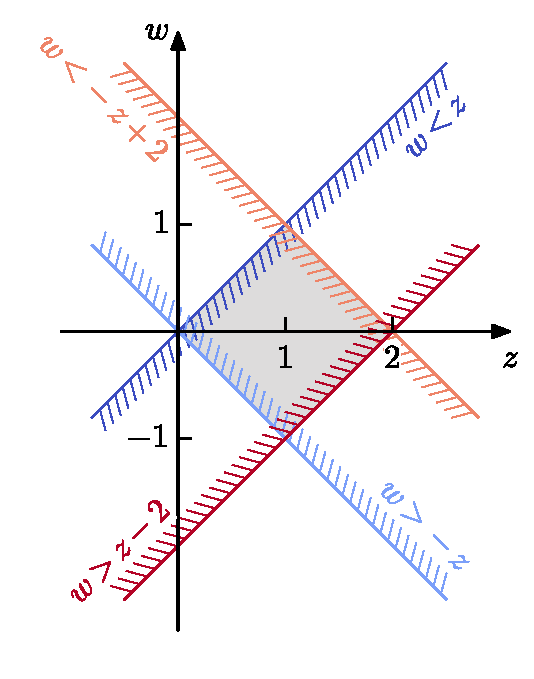
\includegraphics[width=\textwidth]{figuras/joint_distribution_sum_sub_v3.pdf}
  \end{minipage}\hfill
  \begin{minipage}[c]{0.57\textwidth}
    \caption{
       Región del plano \((z,\,w)\) donde \(f_{zw}(z,\,w)\) no es nula. Consiste en la intersección de los semiplanos determinados por las condiciones \(0<z+w<2\) y \(0<z-w<2\).
    } \label{fig:joint_distribution_sum_sub_v3}
  \end{minipage}
\end{figure}
Finalmente, se tiene que
\[
 f_{xy}(x,\,y)=f_x(x)f_y(y)=1,\qquad 0<x<1,\, 0<y<1.
\]
Sustituyendo estos resultados en la ecuación \ref{eq:joint_density_two_funcions_two_rv}, se concluye que
\[
 f_{zw}(z,\,w)=\left\{\begin{array}{ll}
  1/2, &  0<z+w<2,\,0<z-w<2\\
  0, & \textrm{en otro caso.}
 \end{array} \right.
\]

\begin{figure}[!htb]
\begin{center}
 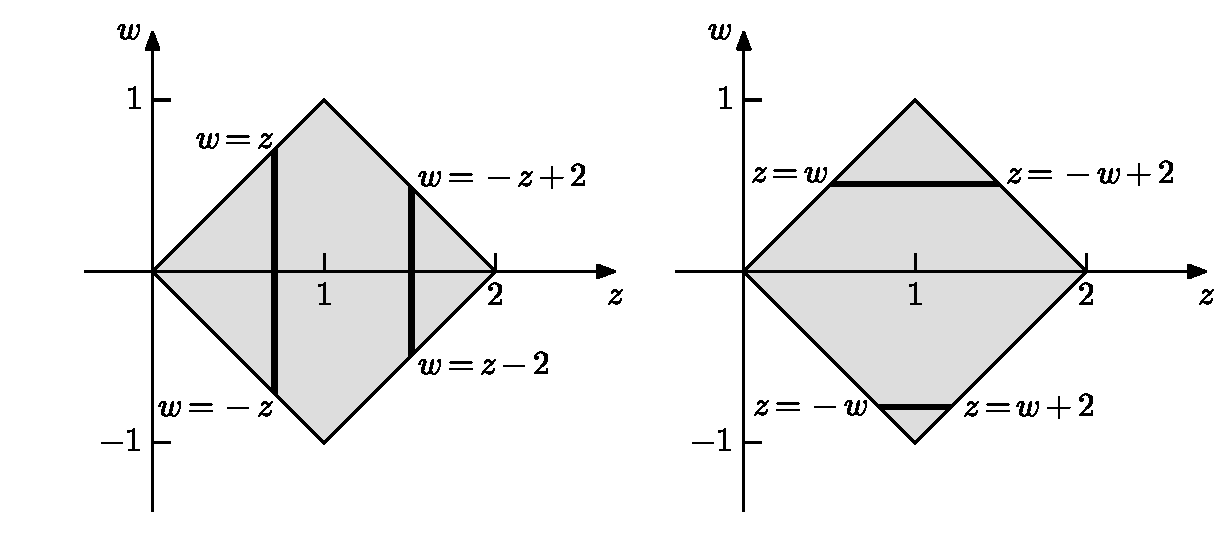
\includegraphics[width=0.9\columnwidth]{figuras/joint_distribution_sum_sub_marginals.pdf}
\caption{\label{fig:joint_distribution_sum_sub_marginals} Límites de integración de \(f_{zw}(z,\,w)\) para el cálculo de las densidades marginales. Se observa que los límites de integración dependen del valor de la variable de la que se calcula el marginal. A la izquierda se muestran los intervalos de integración para calcular la densidad marginal de \(z\). Se distinguen dos casos: si \(0<z<1\), los límites de integración son \(-z<w<z\) y si \(1<z<2\), los límites de integración son \(z-2<w<-z+2\). A la derecha, se muestran los intervalos de integración para calcular el marginal de \(w\). Si \(0<w<1\), los límites de integración son \(w<z<-w+2\), y si \(-1<w<0\), los límites de integración son \(-w<z<w+2\). En este caso, esto se puede resumir como \(|w|<z<2-|w|\) para \(-1<w<1\).}
\end{center}
\end{figure}
La densidad marginal \(f_z(z)\) se obtiene integrando \(f_{zw}(z,\,w)\) respecto a \(w\). Para esto, hay que tener en cuenta que los límites de integración dependen del valor de \(z\), como se muestra en la figura \ref{fig:joint_distribution_sum_sub_marginals}. 
De esta forma,
\begin{equation}\label{eq:joint_distribution_sum_sub_z}
 f_z(z)=\int f_{zw}(z,\,w)\,dw
\def\arraystretch{2}\arraycolsep=10pt
 =\left\{\begin{array}{ll}
   \displaystyle\int_{-z}^{z}\dfrac{1}{2}\,dw=z, &  0<z<1\\
   \displaystyle\int_{z-2}^{-z+2}\dfrac{1}{2}\,dw=-z+2, & 1<z<2\\ 
   0 & \textrm{en otro caso.}
 \end{array} \right., 
\end{equation}
y la densidad marginal de \(w\) es
\[
 f_w(w)=\int f_{zw}(z,\,w)\,dz=\int_{|w|}^{2-|w|}\dfrac{1}{2}\,dz=\frac{z}{2}\,z\bigg|_{|w|}^{2-|w|}
 =\frac{2-|w|}{2}-\frac{|w|}{2}=1-|w|,
\]
si \(-1<w<1\). Es decir
\begin{equation}\label{eq:joint_distribution_sum_sub_w}
f_w(w)=\int f_{zw}(z,\,w)\,dz
 =\left\{\begin{array}{ll}
   1-|w|, &  -1<w<1\\
   0 & \textrm{en otro caso.}
 \end{array} \right..
\end{equation}
De las ecuaciones \ref{eq:joint_distribution_sum_sub_z} y \ref{eq:joint_distribution_sum_sub_w} se deduce que
\[
 f_z(z)f_w(w)=
\arraycolsep=10pt
 \left\{\begin{array}{ll}
   z(1-|w|), &  0<z<1,\,-1<w<1\\
   (2-z)(1-|w|), & 1<z<2,\,-1<w<1\\
   0 & \textrm{en otro caso.}
 \end{array} \right., 
\]
y comparando este resultado con \(f_{zw}(z,\,w)\), se ve que \(f_{zw}(z,\,w)\neq f_z(z)f_w(w)\), lo que indica que las variables aleatorias \(\z\) y \(\w\) no son independientes.

Se calculará ahora la covarianza entre \(\z\) y \(\w\) para estudiar la correlación. Por un lado, se tiene que
\begin{align*}
 E\{\z\w\}&=E\{(\x+\y)(\x-\y)\}\\
   &=E\{\x^2-\x\y+\y\x-\y^2\}\\
   &=E\{\x^2-\y^2\}\\
   &\overset{(a)}{=}E\{\x^2\}-E\{\y^2\}\\
   &\overset{(b)}{=}0,
\end{align*}
donde en \((a)\) se empleó la propiedad de linealidad de la esperanza y en \((b)\) se usó que \(E\{\x^2\}=E\{\y^2\}\) debido a que \(\x\) y \(\z\) tienen igual densidad de probabilidad. Esto indica que las variables aleatorias \(\z\) y \(\w\) son ortogonales. Por otro lado, se ve que
\[
 E\{\w\}=E\{\x-\y\}=E\{\x\}-E\{\y\}=0.
\]
A partir de estos dos resultados, se llega a que
\[
 C_{zw}=E\{\z\w\}-E\{\z\}E\{\w\}=0,
\]
implicando que las variables aleatorias \(\z\) y \(\w\) son no correlacionadas. Se concluye que \(\z\) y \(\w\) son variables aleatorias que no son independientes pero son no correlacionadas.

Las densidades \(f_z(z)\) y \(f_w(w)\) de las ecuaciones \ref{eq:joint_distribution_sum_sub_z} y \ref{eq:joint_distribution_sum_sub_w} se obtuvieron como los marginales de \(f_{zw}(z,\,w)\). Como \(\z=\x+\y\), \(f_z(z)\) se podría haber calculado como en la sección \ref{sec:rv_sum_density}, donde se concluyó que la densidad de la suma de dos variables aleatorias independientes es la convolución de las densidades. Así,
\[
 f_z(z)=\int_{-\infty}^{\infty}f_x(z-y)f_y(y)\,dy.
\]
Como
\[
  f_x(x)=
 \left\{\begin{array}{ll}
   1, &  0<x<1\\
   0, & \textrm{en otro caso.}
 \end{array} \right., 
\]
se tiene que
\[
  f_x(z-y)=
 \left\{\begin{array}{ll}
   1, &  0<z-y<1\\
   0, & \textrm{en otro caso.}
 \end{array} \right.=
 \left\{\begin{array}{ll}
   1, &  z-1<y<z\\
   0, & \textrm{en otro caso.}
 \end{array} \right..
\]
Por lo tanto,
\begin{equation}\label{eq:joint_distribution_sum_sub_fz_deduction}
  f_x(z-y)f_y(y)=
 \left\{\begin{array}{llclc}
   0 &  \textrm{en} &-\infty<y<\infty & \textrm{si} & z<0\textrm{ o }z>2\\
   1 &  \textrm{en} & 0<y<z & \textrm{si} & 0<z<1\\
   1 &  \textrm{en} & z-1<y<1 & \textrm{si} & 1<z<2
 \end{array}\right., 
\end{equation}
como se muestra en la figura \ref{fig:joint_distribution_sum_sub_marginals_convolutions}, e integrando se obtiene que
\[
 f_z(z)=\int_{-\infty}^{\infty}f_x(z-y)f_y(y)\,dy
\def\arraystretch{2}\arraycolsep=10pt
 =\left\{\begin{array}{ll}
   \displaystyle\int_{0}^{z}1\,dy=z, &  0<z<1\\
   \displaystyle\int_{z-1}^{1}1\,dy=2-z, & 1<z<2\\ 
   0 & \textrm{en otro caso.}
 \end{array} \right., 
\]
resultado que coincide con la ecuación \ref{eq:joint_distribution_sum_sub_z}.
Para calcular la densidad \(f_w(w)\), procediendo como en la sección \ref{sec:rv_sum_density}, se puede demostrar que si \(\w=\x-\y\),
\[
 f_w(w)=\int_{-\infty}^{\infty}f_{xy}(y+w,y)\,dy=\int_{-\infty}^{\infty}f_{xy}(x,x-w)\,dx,
\]
y si \(\x\) e \(\y\) son independientes, queda
\begin{equation}\label{eq:pdf_of_subtract_of_two_independents_rv}
 f_w(w)=\int_{-\infty}^{\infty}f_x(y+w)f_y(y)\,dy=\int_{-\infty}^{\infty}f_x(x)f_y(x-w)\,dx,
\end{equation}
que es la convolución entre las funciones \(f_x(\tau)\) y \(f_y(-\tau)\).
Observando el que
\[
  f_y(x-w)=
 \left\{\begin{array}{ll}
   1, &  0<x-w<1\\
   0, & \textrm{en otro caso.}
 \end{array} \right.=
 \left\{\begin{array}{ll}
   1, &  w<x<1+w\\
   0, & \textrm{en otro caso.}
 \end{array} \right.,
\]
el integrando de \(f_w(w)\) es
\begin{equation}\label{eq:joint_distribution_sum_sub_fw_deduction}
   f_x(x)f_y(x-w)=
 \left\{\begin{array}{llclc}
   0 &  \textrm{en} &-\infty<x<\infty & \textrm{si} & w<-1\textrm{ o }w>1\\
   1 &  \textrm{en} & 0<x<w+1 & \textrm{si} & -1<w<0\\
   1 &  \textrm{en} & w<x<1 & \textrm{si} & 0<w<1
 \end{array}\right.,
\end{equation}
como se muestra en la figura \ref{fig:joint_distribution_sum_sub_marginals_convolutions},
por lo que
\[
 f_w(w)=\int_{-\infty}^{\infty}f_x(x)f_y(x-w)\,dx
\def\arraystretch{2}\arraycolsep=9pt
 =\left\{\begin{array}{ll}
   \displaystyle\int_{0}^{w+1}1\,dx=w+1, &  -1<w<0\\
   \displaystyle\int_{w}^{1}1\,dx=1-w, & 0<w<1\\ 
   0 & \textrm{en otro caso}
 \end{array} \right., 
\]
coincidiendo con la ecuación \ref{eq:joint_distribution_sum_sub_w}. Las distribuciones marginales \(f_z(z)\) y \(f_w(w)\) se muestran en la figura \ref{fig:joint_distribution_sum_sub_marginals_convolutions}.
\begin{figure}[!htb]
\begin{center}
 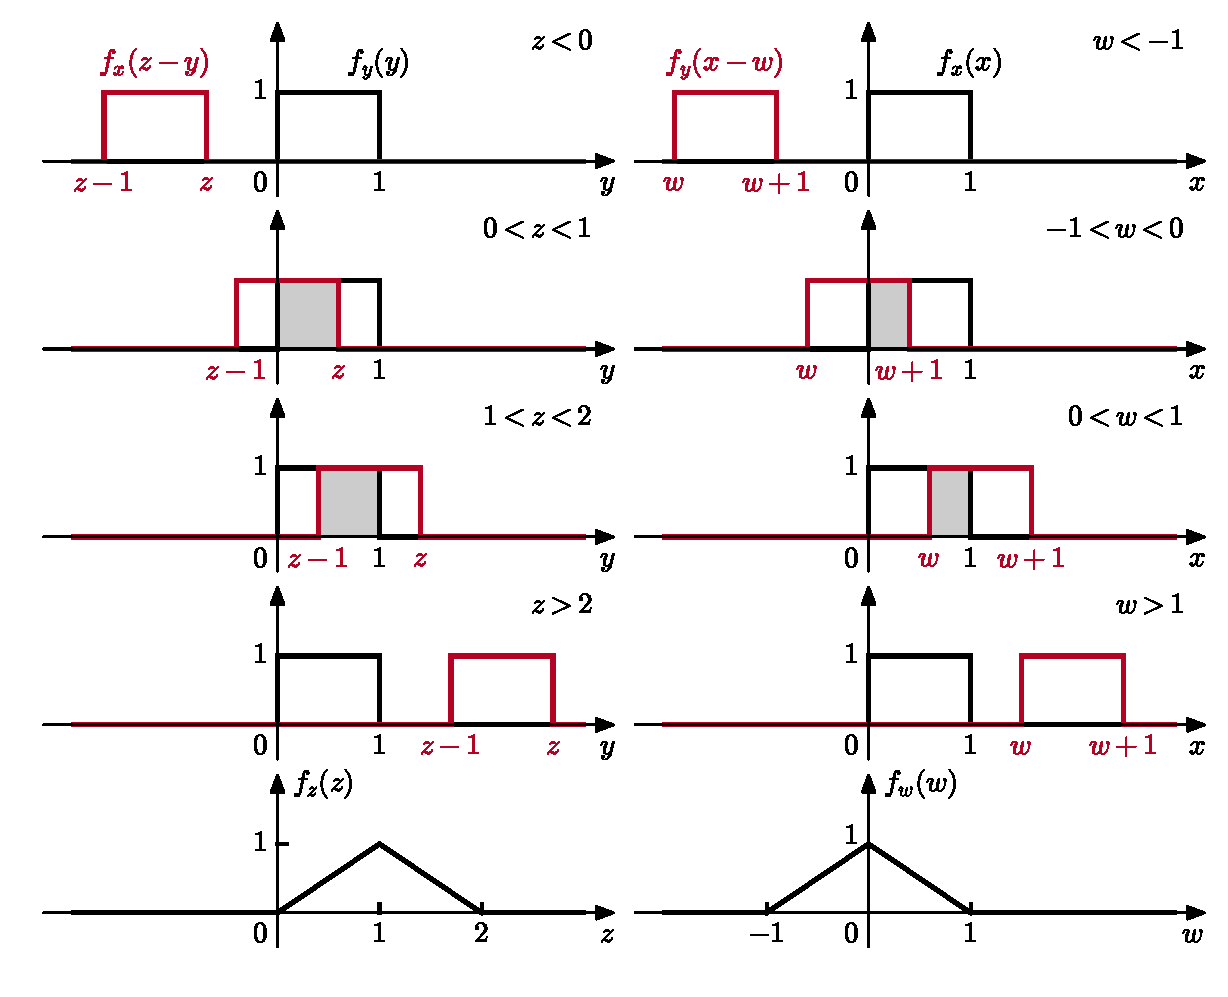
\includegraphics[width=1\columnwidth]{figuras/joint_distribution_sum_sub_marginals_convolutions.pdf}
\caption{\label{fig:joint_distribution_sum_sub_marginals_convolutions} Deducción de las ecuaciones \ref{eq:joint_distribution_sum_sub_fz_deduction} y \ref{eq:joint_distribution_sum_sub_fw_deduction}. A la izquierda se muestra la deducción de la densidad \(f_z(z)\) de \(\z=\x+\y\) a partir de la ecuación \ref{eq:pdf_of_sum_of_two_independents_rv} para el caso en que \(\x\sim U(0,\,1)\) e \(\y\sim U(0,\,1)\). \(f_z(z)\) es la convolución entre \(f_x(x)\) y \(f_y(y)\), es decir, la integral del producto de las funciones \(f_y(y)\) y \(f_x(z-y)\), las cuales se muestran para distintos valores de \(z\) y consiste en el área de la región sombreada. A la derecha se muestra la deducción de la densidad \(f_w(w)\) de \(\w=\x-\y\), que está dada por la ecuación \ref{eq:pdf_of_subtract_of_two_independents_rv}.}
\end{center}
\end{figure}

\paragraph{Varianza de la suma de dos variables aleatorias}

Sea \(\z=\x+\y\). Por la propiedad de linealidad de la esperanza, se cumple que \(\eta_z=\eta_x+\eta_y\). Por lo tanto, la varianza de \(\z\) es
\begin{align}\label{eq:sum_of_rv_variance}
 \sigma_z^2&=E\{(\z-\eta_z)^2\}\nonumber\\
   &=E\{\left[(\x+\y)-(\eta_x+\eta_y)\right]^2\}\nonumber\\
   &\overset{(a)}{=}\sigma_x^2+2C_{xy}+\sigma_y^2\nonumber\\
   &\overset{(b)}{=}\sigma_x^2+2\rho_{xy}\sigma_x\sigma_y+\sigma_y^2,
\end{align}
donde en \((a)\) se empleó la igualdad de la ecuación \ref{eq:covariance_rho_relation_deduction} con \(a=1\) y en \((b)\) la definición del coeficiente de correlación, dado por la ecuación \ref{eq:correlation_coefficient_definition}. Este resultado indica que si \(\rho_{xy}=0\), se cumple que
\[
 \sigma_z^2=\sigma_x^2+\sigma_y^2.
\]
Se concluye que si dos variables aleatorias son no correlacionadas, la varianza de su suma es la suma de las varianzas. Como dos variables aleatorias independientes son no correlacionadas, esto también es cierto para el caso de variables aleatorias independientes.

\paragraph{Momentos}

El valor
\[
 m_{kr}=E\{\x^k\y^r\}=\int_{-\infty}^{\infty}x^ky^rf_{xy}(x,\,y)\,dx\,dy
\]
es el momento conjunto de orden \(n=k+r\) de las variables aleatorias \(\x\) e \(\y\). De esta forma, los momentos de primer orden son \(m_{10}=\eta_x\) y \(m_{01}=\eta_y\) y los momentos de segundo orden son
\[
 m_{20}=E\{\x^2\},\qquad m_{11}=E\{\x\y\},\qquad m_{02}=E\{\y^2\}.
\]

Los momentos centrales son los momentos de \(\x-\eta_x\) y \(\y-\eta_y\),
\[
 \mu_{kr}=E\{(\x-\eta_x)^k(\y-\eta_y)^r\}=\int_{-\infty}^{\infty}(\x-\eta_x)^k(\y-\eta_y)^rf_{xy}(x,\,y)\,dx\,dy.
\]
Así, \(\mu_{10}=\mu_{01}=0\) y 
\[
 \mu_{11}=C_{xy},\qquad \mu_{20}=\sigma_x^2,\qquad \mu_{02}=\sigma_y^2.
\]

\section{Funciones características conjuntas}

La función característica conjunta de las variables aleatorias \(\x\) e \(\y\) es por definición
\begin{equation}\label{eq:joint_characteristic_function_definition}
 \Phibf(\omega_1,\,\omega_2)=\int_{-\infty}^{\infty}\int_{-\infty}^{\infty}f(x,\,y)e^{j(\omega_1x+\omega_2y)}\,dx\,dy.
\end{equation}
Esto es la transformada de Fourier de dos dimensiones de \(f(x,\,y)\). Aplicando la fórmula de inversión de la transformada de Fourier, se ve que se cumple que
\begin{equation}\label{eq:joint_characteristic_inverse_function}
 f(x,\,y)=\frac{1}{4\pi^2}\int_{-\infty}^{\infty}\int_{-\infty}^{\infty}\Phibf(\omega_1,\,\omega_2)e^{-j(\omega_1x+\omega_2y)}\,d\omega_1\,d\omega_2.
\end{equation}
De esta forma,
\[
 \Phibf(\omega_1,\,\omega_2)=E\{e^{j(\omega_1\x+\omega_2\y)}\}.
\]
La función característica conjunta logarítmica se define como
\[
 \Psibf(\omega_1,\,\omega_2)=\ln\Phibf(\omega_1,\,\omega_2).
\]

Las funciones características marginales (ecuación \ref{eq:characteristic_function})
\[
 \Phibf_x(\omega)=E\{e^{j\omega\x}\},\qquad \Phibf_y(\omega)=E\{e^{j\omega\y}\}
\]
pueden expresarse en función de la función característica conjunta como
\[
 \Phibf_x(\omega)=\Phibf(\omega,\,0),\qquad \Phibf_y(\omega)=\Phibf(0,\,\omega),
\]
ya que, 
\begin{align*}
 \Phibf(\omega,\,0)&=\int_{-\infty}^{\infty}\int_{-\infty}^{\infty}f(x,\,y)e^{j\omega_1x}\,dx\,dy\\
  &=\int_{-\infty}^{\infty}\left(\int_{-\infty}^{\infty}f(x,\,y)\,dy\right)e^{j\omega_1x}\,dx\\
  &=\int_{-\infty}^{\infty}f_x(x)e^{j\omega_1x}\,dx\\
  &=\Phibf_x(\omega).
\end{align*}

Notar que si \(\z=a\x+b\y\),
\begin{equation}\label{eq:characteristic_function_linear_combination}
 \Phibf_z(\omega)=E\{e^{j(a\x+b\y)\omega}\}=\Phibf(a\omega,\,b\omega).
\end{equation}

\subsection{Independencia y convolución}\label{sec:two_rv_independence_and_convolution}

Si las variables aleatorias \(\x\) e \(\y\) son independientes, se cumple que (ecuación \ref{eq:independent_rv_mean_functions_product})
\[
 E\{e^{j(\omega_1\x+\omega_2\y)}\}=E\{e^{j\omega_1\x}\}E\{e^{j\omega_2\y}\}
\]
y por lo tanto, la función característica conjunta es
\begin{equation}\label{eq:independent_rv_characteristic_function}
 \Phibf(\omega_1,\,\omega_2)=\Phibf_x(\omega_1)\Phibf_y(\omega_2).
\end{equation}
Recíprocamente, si se cumple la ecuación \ref{eq:independent_rv_characteristic_function}, las variables aleatorias \(\x\) e \(\y\) son independientes. Para ver esto, se parte sustituyendo la ecuación \ref{eq:independent_rv_characteristic_function} en la fórmula de inversión,
\begin{align*}
 f(x,\,y)&=\frac{1}{4\pi^2}\int_{-\infty}^{\infty}\int_{-\infty}^{\infty}\Phibf_x(\omega_1)\Phibf_y(\omega_2)e^{-j(\omega_1x+\omega_2y)}\,d\omega_1\,d\omega_2\\
 &=\left(\frac{1}{2\pi}\int_{-\infty}^{\infty}\Phibf_x(\omega_1)e^{-j\omega_1x}\,d\omega_1\right)  \left(\frac{1}{2\pi}\int_{-\infty}^{\infty}\Phibf_y(\omega_2)e^{-j\omega_2y}\,d\omega_2\right)\\
 &=f_x(x)f_y(y),
\end{align*}
donde en la última igualdad se usó la fórmula de inversión de la función característica de una variable aleatoria (ecuación \ref{eq:characteristic_function_inversion}). Se concluye que como \(f(x,\,y)=f_x(x)f_y(y)\), \(\x\) e \(\y\) son independientes.

\paragraph{Teorema de la convolución}

Si las variables aleatorias \(\x\) e \(\y\) son independientes y \(\z=\x+\y\), se cumple que
\[
 E\{e^{j\omega\z}\}=E\{e^{j\omega(\x+\y)}\}=E\{e^{j\omega\x}\}E\{e^{j\omega\y}\}
\]
y por lo tanto
\begin{equation}\label{eq:characteristic_function_convolution_theorem}
 \Phibf_z(\omega)=\Phibf_x(\omega)\Phibf_y(\omega),\qquad \Psibf_z(\omega)=\Psibf_x(\omega)+\Psibf_y(\omega)
\end{equation}

Como se vio en la sección \ref{sec:rv_sum_density}, la densidad \(f_z(z)\) de \(\z\) es la convolución de las densidades \(f_x(x)\) y \(f_y(y)\). Se concluye que la función característica de la convolución de dos densidades es el producto de las funciones características. 

Se demostrará nuevamente este resultado empleando propiedades de la transformada de Fourier. Sean \(f_x(x)\) y \(f_y(y)\) las densidades de probabilidad de las variables aleatorias \(\x\) e \(\y\) respectivamente, y se considera una variable aleatoria \(\z\) con densidad de probabilidad la convolución entre \(f_x(x)\) y \(f_y(y)\). De esta forma, como indica la ecuación \ref{eq:pdf_of_sum_of_two_independents_rv},
\[
 f_z(z)=\int_{-\infty}^{\infty}f_x(x)f_y(z-x)\,dx.
\]
Se demostrará que la función característica de \(\z\) es \(\Phibf_z(\omega)=\Phibf_x(\omega)\Phibf_y(\omega)\). Partiendo de la definición de la función característica, se tiene que
\begin{align*}
 \Phibf_z(\omega)&=\int_{-\infty}^{\infty}f_z(z)e^{j\omega z}\,dz\\
   &\overset{(a)}{=}\int_{-\infty}^{\infty}\left[\int_{-\infty}^{\infty}f_x(x)f_y(z-x)\,dx\right]e^{j\omega z}\,dz\\
   &\overset{(b)}{=}\int_{-\infty}^{\infty}f_x(x)\left[\int_{-\infty}^{\infty}f_y(z-x)e^{j\omega z}\,dz\right]\,dx\\
   &\overset{(c)}{=}\int_{-\infty}^{\infty}f_x(x)\left[\int_{-\infty}^{\infty}f_y(y)e^{j\omega(x+y)}\,dy\right]\,dx\\
   &=\int_{-\infty}^{\infty}f_x(x)e^{j\omega x}\,dx\int_{6-\infty}^{\infty}f_y(y)e^{j\omega y}\,dy\\
   &=\Phibf_x(\omega)\Phibf_y(\omega),
\end{align*}
donde en \((a)\) se sustituyó \(f_z(z)\) por la convolución, en \((b)\) se intercambió el orden de integración y en \((c)\) se realizó el cambio de variable \(z=x+y\). De forma análoga, puede demostrarse lo recíproco, esto es, si la función característica de \(\z\) es \(\Phibf_z(\omega)=\Phibf_x(\omega)\Phibf_y(\omega)\), la densidad de \(\z\) es la convolución entre las densidades de \(\x\) e \(\y\). Para ver esto, se parte de la transformada inversa de la función característica y se opera de la siguiente forma,
\begin{align*}
 f_z(z)&=\frac{1}{2\pi}\int_{-\infty}^{\infty}\Phibf_z(\omega)e^{-j\omega z}\,d\omega\\
   &=\frac{1}{2\pi}\int_{-\infty}^{\infty}\Phibf_x(\omega)\Phibf_y(\omega)e^{-j\omega z}\,d\omega\\
   &\overset{(a)}{=}\frac{1}{2\pi}\int_{-\infty}^{\infty}\left[\int_{-\infty}^{\infty}f_x(x)e^{j\omega x}\,dx\right]\Phibf_y(\omega)e^{-j\omega z}\,d\omega\\
   &\overset{(b)}{=}\int_{-\infty}^{\infty}f_x(x)\left[\frac{1}{2\pi}\int_{-\infty}^{\infty}\Phibf_y(\omega)e^{-j\omega (z-x)}\,d\omega\right]\,dx\\
   &\overset{(c)}{=}\int_{-\infty}^{\infty}f_x(x)f_y(z-x)\,dx,
\end{align*}
donde en \((a)\) se sustituyó \(\Phibf_x(\omega)\) por su definición, en \((b)\) se intercambió el orden de integración y en \((c)\) se tuvo en cuenta que el término entre paréntesis rectos es la transformada inversa de la función característica \(\Phibf_y(\omega)\) evaluada en \(z-x\), es decir, \(f_y(z-x)\).

\paragraph{Ejemplo: variables aleatorias normales independientes}

Como se indicó previamente (ver la ecuación \ref{eq:jointly_normal_linear_transformation}), si las variables aleatorias \(\x\) e \(\y\) son conjuntamente normales, cualquier combinación lineal \(a\x+b\y\) es una variable aleatoria normal. Se demostrará el siguiente caso particular de este resultado: si las variables aleatorias \(\x\) e \(\y\) son normales e independientes, su suma \(\z=\x+\y\) también es normal. Para demostrarlo, se parte de las funciones características de \(\x\) e \(\y\), que por ser normales son (ver la ecuación \ref{eq:normal_rv_characteristic_function}),
\[
 \Phi_x(\omega)=e^{j\eta_x\omega-\frac{1}{2}\sigma_x^2\omega^2},\qquad \Phi_y(\omega)=e^{j\eta_y\omega-\frac{1}{2}\sigma_y^2\omega^2}.
\]
Por ser variables aleatorias independientes, por el teorema de la convolución dado por la ecuación \ref{eq:characteristic_function_convolution_theorem}, se cumple que
\[
 \Phi_z(\omega)=\Phi_x(\omega)\Phi_y(\omega)=\exp\left\{j(\eta_x+\eta_y)\omega-\frac{1}{2}(\sigma_x^2+\sigma_y^2)\omega^2\right\},
\]
que es la función característica de una variable aleatoria normal de media \(\eta_x+\eta_y\) y varianza \(\sigma_y^2+\sigma_y^2\). Se concluye que \(\z\sim N(\eta_x+\eta_y,\,\sigma_x^2+\sigma_y^2)\).

Puede demostrarse que lo recíproco también es cierto (teorema de descomposición de Cramér
\footnote{Ver \href{https://en.wikipedia.org/wiki/Cram\%C3\%A9r\%27s_theorem\#Normal_random_variables}{\texttt{https://en.wikipedia.org/wiki/Cramér's\_theorem\#Normal\_random\_variables}}}): si las variables aleatorias \(\x\) e \(\y\) son independientes y su suma es normal, entonces \(\x\) e \(\y\) son normales. Esto es equivalente a afirmar que la convolución de dos densidades es normal si y solo si ambas densidades son normales. También se puede demostrar que si \(\x\) e \(\y\) son variables aleatorias normales independientes, se cumple también que \(\x+\y\) y \(\x-\y\) también son independientes y normales. En este caso, el recíproco también es cierto (teorema de Bernstein\footnote{Ver \url{https://en.wikipedia.org/wiki/Normal_distribution\#Bernstein's_theorem}}): si \(\x\) e \(\y\) son independientes e idénticamente distribuidas y si \(\x+\y\) y \(\x-\y\) también son independientes, necesariamente las variables aleatorias \((\x,\,\y,\,\x+\y,\,\x-\y)\) son normales.

En el caso en que \(\z=a\x+b\y\), se cumple que
\[
 \Phi_z(\omega)\overset{(a)}{=}\Phi_{xy}(a\omega,\,b\omega)\overset{(b)}{=}\Phi_x(a\omega)\Phi_y(b\omega),
\]
donde en \((a)\) se empleó el resultado de la ecuación \ref{eq:characteristic_function_linear_combination} y en \((b)\) se consideró que \(\x\) e \(\y\) son variables aleatorias independientes. De esta forma,
\[
 \Phi_z(\omega)=\exp\left\{j(a\eta_x+b\eta_y)\omega-\frac{1}{2}(a^2\sigma_x^2+b^2\sigma_y^2)\omega^2\right\},
\]
por lo que \(\z\sim N(a\eta_x+b\eta_y,\,a^2\sigma_x^2+b^2\sigma_y^2)\).



\paragraph{Variables aleatorias conjuntamente normales}
Sean \(\x\) e \(\y\) variables aleatorias conjuntamente normales con densidad \(N(\eta_1,\,\eta_2,\,\sigma_1^2,\,\sigma_2^2,\,r)\). Su función característica conjunta está dada por
\begin{equation}\label{eq:characteristic_function_jointly_normal}
 \Phibf(\omega_1,\,\omega_2)=e^{j(\eta_1\omega_1+\eta_2\omega_2)}e^{-(\omega_1^2\sigma_1^2+2r\sigma_1\sigma_2\omega_1\omega_2+\omega_2^2\sigma_2^2)/2}.
\end{equation}
Una forma de demostrarlo, es insertando la densidad de probabilidad conjunta, dada por las ecuaciones \ref{eq:joint_normal_pdf1} y \ref{eq:joint_normal_pdf2}, en la definición de la función característica conjunta (ecuación \ref{eq:joint_characteristic_function_definition}) y calcular la integral. Esto se hará mas adelante. Otra forma mas simple, es la siguiente. Se considera la variable aleatoria \(\z=\omega_1\x+\omega_2\y\), que por ser una combinación lineal de variables aleatorias normales, es normal, y por lo tanto, su función característica es (ecuación \ref{eq:normal_rv_characteristic_function})
\[
 \Phibf_z(\omega)=e^{j\eta_z\omega-\sigma_z^2\omega^2/2}.
\]
La media de \(\z\) es
\[
 \eta_z=\omega_1\eta_1+\omega_2\eta_2
\]
y su varianza es
\begin{align*}
\sigma_z^2&=E\{\left[(\omega_1\x+\omega_2\y)-(\omega_1\eta_1+\omega_2\eta_2)\right]^2\}\\
  &=E\{\left[(\omega_1\x-\omega_1\eta_1)+(\omega_2\y-\omega_2\eta_2)\right]^2\}\\
  &=E\{\left[\omega_1(\x-\eta_1)+\omega_2(\y-\eta_2)\right]^2\}\\
  &=E\{\omega_1^2(\x-\eta_1)^2+2\omega_1\omega_2(\x-\eta_1)(\y-\eta_2)+\omega_2^2(\y-\eta_2)^2\}\\
  &=\omega_1^2E\{(\x-\eta_1)^2\}+2\omega_1\omega_2E\{(\x-\eta_1)(\y-\eta_2)\}+\omega_2^2E\{(\y-\eta_2)^2\}\\
  &=\omega_1^2\sigma_1^2+2\omega_1\omega_2C_{xy}+\omega_2^2\sigma_2^2
\end{align*}
concluyendo que
\[
 \sigma_z^2=\omega_1^2\sigma_1^2+2r\omega_1\omega_2\sigma_1\sigma_2+\omega_2^2\sigma_2^2.
\]
Además, como indica la ecuación \ref{eq:characteristic_function_linear_combination}, se cumple que
\[
 \Phibf_z(\omega)=\Phibf(\omega_1\omega,\,\omega_2\omega),
\]
por lo que con \(\omega=1\) se llega al resultado que se quería demostrar.

Se demostrará a continuación el mismo resultado resolviendo explícitamente la integral de la definición de la función característica. Si bien esta demostración es mas larga, tiene la ventaja de que no hay que emplear la hipótesis de que la combinación lineal de variables aleatorias normales es normal. La demostración aquí presentada está basada en \cite{weisstein18bivarite}. Se parte sustituyendo la densidad de probabilidad conjunta \(N(\eta_1,\,\eta_2,\,\sigma_1^2,\,\sigma_2^2,\,r)\), dada por las ecuaciones \ref{eq:joint_normal_pdf1} y \ref{eq:joint_normal_pdf2}, en la función característica, dada por la ecuación \ref{eq:joint_characteristic_function_definition},
\begin{align*}
 \Phi(\omega_1,\,\omega_2)&=\int_{-\infty}^{\infty}\int_{-\infty}^{\infty}f(x,\,y)\exp\{j(\omega_1x+\omega_2y)\}\,dx\,dy\\
 &=A\int_{-\infty}^{\infty}\int_{-\infty}^{\infty}\exp\{j(\omega_1x+\omega_2y)\}\exp\bigg\{-\frac{1}{2(1-r^2)}\times\\
 & \qquad\quad\bigg[\frac{(x-\eta_1)^2}{\sigma_1^2}-2r\frac{(x-\eta_1)(y-\eta_2)}{\sigma_1\sigma_2}+\frac{(y-\eta_2)^2}{\sigma_2^2}\bigg]\bigg\}\,dx\,dy,
\end{align*}
donde
\[
 A=\frac{1}{2\pi\sigma_1\sigma_2\sqrt{1-r^2}}.
\]
Realizando el cambio de variable \(u=x-\eta_1\) y \(w=y-\eta_2\) se obtiene que
\begin{align*}
 \Phi(\omega_1,\,\omega_2)&= A\int_{-\infty}^{\infty}\int_{-\infty}^{\infty}\exp\{j[\omega_1(u+\eta_1)+\omega_2(w+\eta_2)]\}\times\\
 & \qquad\quad\exp\left\{-\frac{1}{2(1-r^2)}\left[\frac{u^2}{\sigma_1^2}-2r\frac{uw}{\sigma_1\sigma_2}+\frac{w^2}{\sigma_2^2}\right]\right\}\,du\,dw\\
 &=A\exp\{j(\omega_1\eta_1+\omega_2\eta_2)\}\int_{-\infty}^{\infty}\int_{-\infty}^{\infty}\exp\{j(\omega_1u+\omega_2w)\}\times\\
 & \qquad\quad\exp\left\{-\frac{1}{2(1-r^2)}\left[\frac{u^2}{\sigma_1^2}-2r\frac{uw}{\sigma_1\sigma_2}+\frac{w^2}{\sigma_2^2}\right]\right\}\,du\,dw\\
 &=A'\int_{-\infty}^{\infty}\int_{-\infty}^{\infty}\exp\{j(\omega_1u+\omega_2w)\}\times\\
 & \qquad\quad\exp\left\{-\frac{1}{2(1-r^2)}\left[\frac{u^2}{\sigma_1^2}-2r\frac{uw}{\sigma_1\sigma_2}+\frac{w^2}{\sigma_2^2}\right]\right\}\,du\,dw,
\end{align*}
donde en la última igualdad se definió
\begin{equation}\label{eq:normal_joint_characteristic_function_deduction_tmp3}
 A'=A\exp\{j(\omega_1\eta_1+\omega_2\eta_2)\}=\frac{\exp\{j(\omega_1\eta_1+\omega_2\eta_2)\}}{2\pi\sigma_1\sigma_2\sqrt{1-r^2}}.
\end{equation}
La integral doble puede separarse como
\begin{equation}\label{eq:normal_joint_characteristic_function_deduction_tmp1}
 \begin{aligned}
 \Phi(\omega_1,\,\omega_2)&=A'\int_{-\infty}^{\infty}e^{j\omega_2w}\exp\left\{-\frac{1}{2(1-r^2)}\,\frac{w^2}{\sigma_2^2}\right\}\times\\
 &\qquad\left(\int_{-\infty}^{\infty}e^{j\omega_1u}
 \exp\left\{-\frac{1}{2(1-r^2)}\left[\frac{u^2}{\sigma_1^2}-2r\frac{uw}{\sigma_1\sigma_2}\right]\right\}\,du\right)\,dw.
\end{aligned}
\end{equation}
Se operará a continuación con la integral interna entre paréntesis. La exponencial de la integral interna puede escribirse como
\[ 
 \exp\left\{-\frac{1}{2(1-r^2)}\left[\frac{u^2}{\sigma_1^2}-2r\frac{uw}{\sigma_1\sigma_2}\right]\right\}=
 \exp\left\{-\frac{1}{2\sigma_1^2(1-r^2)}\left[u^2-\frac{2r\sigma_1w}{\sigma_2}u\right]\right\}.
\]
Empleando la técnica de completar el cuadrado con el término entre paréntesis rectos, éste puede escribirse como
\[
 u^2-\frac{2r\sigma_1w}{\sigma_2}u=\left[u-\frac{r\sigma_1w}{\sigma_2}\right]^2-\frac{r^2\sigma_1^2w^2}{\sigma_2^2}
\]
ya que
\[
 \left[u-\frac{r\sigma_1w}{\sigma_2}\right]^2=u^2-2\frac{r\sigma_1w}{\sigma_2}u+\frac{r^2\sigma_1^2w^2}{\sigma_2^2}.
\]
Por lo tanto, la integral interna puede escribirse como
\[
 \int_{-\infty}^{\infty}e^{j\omega_1u}
 \exp\left\{-\frac{1}{2\sigma_1^2(1-r^2)}\left[u-\frac{r\sigma_1w}{\sigma_2}\right]^2\right\}\exp\left\{\frac{1}{2\sigma_1^2(1-r^2)}\frac{r^2\sigma_1^2w^2}{\sigma_2^2}\right\}\,du
\]
y como la última exponencial no depende de la variable de integración \(u\), puede sacarse fuera de la integral, resultando en
\[
 \exp\left\{\frac{1}{2(1-r^2)}\frac{r^2w^2}{\sigma_2^2}\right\}\int_{-\infty}^{\infty}e^{j\omega_1u}
 \exp\left\{-\frac{1}{2\sigma_1^2(1-r^2)}\left[u-\frac{r\sigma_1w}{\sigma_2}\right]^2\right\}\,du.
\]
Al realizar el cambio de variable \(v=u-r\sigma_1w/\sigma_2\), se obtiene que
\[
 \exp\left\{\frac{1}{2(1-r^2)}\frac{r^2w^2}{\sigma_2^2}\right\}\int_{-\infty}^{\infty}\exp\left\{j\omega_1\left(v+\frac{r\sigma_1w}{\sigma_2}\right)\right\}
 \exp\left\{-\frac{v^2}{2\sigma_1^2(1-r^2)}\right\}\,dv,
\]
es decir,
\[
 \exp\left\{\frac{1}{2(1-r^2)}\frac{r^2w^2}{\sigma_2^2}\right\}\exp\left\{j\omega_1\frac{r\sigma_1w}{\sigma_2}\right\}\int_{-\infty}^{\infty}e^{j\omega_1v}
 \exp\left\{-\frac{v^2}{2\sigma_1^2(1-r^2)}\right\}\,dv,
\]
donde se desarrolló la primer exponencial del integrando y se sacó afuera de la integral el término que no depende de la variable de integración. Sustituyendo este resultado por la integral interna en la ecuación \ref{eq:normal_joint_characteristic_function_deduction_tmp1}, se obtiene que
\begin{align*}
 \Phi(\omega_1,\,\omega_2)&=A'\int_{-\infty}^{\infty}e^{j\omega_2w}\exp\left\{-\frac{1}{2(1-r^2)}\,\frac{w^2}{\sigma_2^2}\right\}
 \bigg(\exp\left\{\frac{1}{2(1-r^2)}\frac{r^2w^2}{\sigma_2^2}\right\}\times\\
 &\qquad\exp\left\{j\omega_1\frac{r\sigma_1w}{\sigma_2}\right\}\int_{-\infty}^{\infty}e^{j\omega_1v}
 \exp\left\{-\frac{v^2}{2\sigma_1^2(1-r^2)}\right\}\,dv\bigg)\,dw,
\end{align*}
y operando, se llega a que
\begin{equation}\label{eq:normal_joint_characteristic_function_deduction_tmp2}
 \begin{aligned}
 \Phi(\omega_1,\,\omega_2)&=A'\int_{-\infty}^{\infty}\exp\left\{jw\left(\omega_1\frac{r\sigma_1}{\sigma_2}+\omega_2\right)\right\}\exp\left\{-\frac{w^2}{2\sigma_2^2}\right\}
 \,dw\,\times\\
 &\qquad\int_{-\infty}^{\infty}\exp\left\{jv\omega_1\right\}
 \exp\left\{-\frac{v^2}{2\sigma_1^2(1-r^2)}\right\}\,dv,
\end{aligned}
\end{equation}
donde como se separó el integrando de la integral doble en \(h(w,\,v)=h_1(w)h_2(v)\), la integral doble se separó en el producto de dos integrales simples, y además se sacaron factores comunes en el exponente de las exponenciales de la primer integral.

Ambas integrales de la ecuación \ref{eq:normal_joint_characteristic_function_deduction_tmp2} son de la forma
\[
 f(b)=\int_{-\infty}^{\infty}e^{-ax^2}e^{jbx}\,dx,
\]
por lo que a continuación, se resolverá esta integral y se aplicará el resultado en la resolución de la ecuación \ref{eq:normal_joint_characteristic_function_deduction_tmp2}.
Teniendo en cuenta que \(e^{jbx}=\cos(bx)+j\sin(bx)\), se ve que
\begin{align}\label{eq:gaussian_integral_cos_tmp1}
 f(b)&=\int_{-\infty}^{\infty}e^{-ax^2}e^{jbx}\,dx\nonumber\\
   &=\int_{-\infty}^{\infty}e^{-ax^2}\cos(bx)\,dx+j\int_{-\infty}^{\infty}e^{-ax^2}\sin(bx)\,dx\nonumber\\
   &\overset{(a)}{=}\int_{-\infty}^{\infty}e^{-ax^2}\cos(bx)\,dx,
\end{align}
donde en \((a)\) se consideró que la segunda integral es nula ya que integrando es una función impar por tratarse del producto de una función par con una función impar. Considérese ahora
\begin{align*}
 f'(b)&=\frac{d}{db}\left(\int_{-\infty}^{\infty}e^{-ax^2}\cos(bx)\,dx\right)\\
   &=\int_{-\infty}^{\infty}e^{-ax^2}\frac{d}{db}\left(\cos(bx)\right)\,dx\\
   &=-\int_{-\infty}^{\infty}e^{-ax^2}x\sin(bx)\,dx\\
   &\overset{(a)}{=}\frac{1}{2a}\,e^{-ax^2}\sin(bx)\bigg|_{-\infty}^{\infty}-\frac{b}{2a}\int_{-\infty}^{\infty}e^{-ax^2}\cos(bx)\,dx\\
   &\overset{(b)}{=}-\frac{b}{2a}\int_{-\infty}^{\infty}e^{-ax^2}\cos(bx)\,dx
\end{align*}
donde en \((a)\) se aplicó integración por partes, \(\int udv=uv-\int vdu\), con \(u=\sin(bx)\) y \(dv=-xe^{-ax^2}\) por lo que \(du=b\cos(bx)\) y \(v=e^{-ax^2}/2a\) y en \((b)\) se tuvo en cuenta que el primer sumando se anula ya que \(\lim_{x\to\pm\infty}e^{-ax^2}\sin(bx)=0\). Comparando este resultado con la ecuación \ref{eq:gaussian_integral_cos_tmp1}, se concluye que
\[
 f'(b)=-\frac{b}{2a}f(b).
\]
Para resolver esta ecuación diferencial, se observa que
\[
 \frac{f'(b)}{f(b)}=\frac{d}{db}\ln f(b)=-\frac{b}{2a},
\]
por lo que integrando respecto a \(b\) se obtiene que
\[
 \ln f(b)=-\frac{b^2}{4a}+C'
\]
y despejando \(f(b)\) se obtiene que
\[
 f(b)=Ce^{-b^2/4a}.
\]
Para determinar la constante \(C\), se evalúa en \(b=0\),
\[
 f(0)=C=\int_{-\infty}^{\infty}e^{-ax^2}\,dx\overset{(a)}{=}\sqrt{\frac{\pi}{a}},
\]
donde en \((a)\) se consideró que la integral es gaussiana por lo que se cumple el resultado de la ecuación \ref{eq:gaussian_integral_with_alpha}. Se concluye que
\begin{equation}\label{eq:gaussian_integral_with_cos}
 \int_{-\infty}^{\infty}e^{-ax^2}e^{jbx}\,dx=\int_{-\infty}^{\infty}e^{-ax^2}\cos(bx)\,dx=\sqrt{\frac{\pi}{a}}e^{-b^2/4a}.
\end{equation}

Aplicando el resultado de la ecuación \ref{eq:gaussian_integral_with_cos} a las integrales  de la ecuación \ref{eq:normal_joint_characteristic_function_deduction_tmp2} con \(a=1/2\sigma^2_2\) y \(b=\omega_1r\sigma_1/\sigma_2+\omega_2\) en la primer integral y \(a=1/[2\sigma_1^2(1-r^2)]\) y \(b=\omega_1\) en la segunda, y reemplazando \(A'\) por su valor, dado por la ecuación \ref{eq:normal_joint_characteristic_function_deduction_tmp3}, se obtiene que
\begin{align*}
 \Phi(\omega_1,\,\omega_2)&=\frac{\exp\{j(\omega_1\eta_1+\omega_2\eta_2)\}}{2\pi\sigma_1\sigma_2\sqrt{1-r^2}}\sqrt{\pi2\sigma_2^2}\exp\left\{-\left(\omega_1\frac{r\sigma_1}{\sigma_2}+\omega_2\right)^2\frac{2\sigma_2^2}{4}\right\}\times\\
 &\qquad\quad \sqrt{\pi2\sigma_1^2(1-r^2)}\exp\left\{-\omega_1^2\frac{2\sigma_1^2(1-r^2)}{4}\right\}\\
  &=\exp\{j(\omega_1\eta_1+\omega_2\eta_2)\}\exp\left\{-\frac{1}{2}\left(\omega_1r\sigma_1+\omega_2\sigma_2\right)^2-\frac{1}{2}\omega_1^2\sigma_1^2(1-r^2)\right\}\\
  &=\exp\{j(\omega_1\eta_1+\omega_2\eta_2)\}\exp\left\{-\frac{1}{2}\left(\omega_1^2r^2\sigma_1^2+\omega_2^2\sigma_2^2+2\omega_1\omega_2r\sigma_1\sigma_2+\omega_1^2\sigma_1^2-\omega_1^2\sigma_1^2r^2\right)\right\}.
\end{align*}
Se concluye que
\[
 \Phi(\omega_1,\,\omega_2)=\exp\{j(\omega_1\eta_1+\omega_2\eta_2)\}\exp\left\{-\frac{1}{2}\left(\omega_1^2\sigma_1^2+2\omega_1\omega_2r\sigma_1\sigma_2+\omega_2^2\sigma_2^2\right)\right\},
\]
que es lo que se quería demostrar.


\subsection{Teorema de los momentos}

La función generadora de momentos de \(\x\) e \(\y\) está dada por
\[
 \Phibf(s_1,\,s_2)=E\{e^{s_1\x+s_2\y}\}.
\]
Teniendo en cuenta la expansión de la función exponencial,
\[
 e^{-x}=\sum_{n=0}^{\infty}\frac{x^n}{n!}
\]
y considerando la linealidad de la esperanza, se ve que
\[
 \Phibf(s_1,\,s_2)=E\{e^{s_1\x+s_2\y}\}=\sum_{n=0}^{\infty}\frac{E\left\{(s_1\x+s_2\y)^n\right\}}{n!},
\]
y usado el teorema del binomio, que indica que
\[
 (x+y)^n=\sum_{k=0}^{n}x^ky^{n-k},
\]
se obtiene que
\begin{align}\label{eq:joint_moment_generating_function}
 \Phibf(s_1,\,s_2)&=\sum_{n=0}^{\infty}\frac{1}{n!}\sum_{k=0}^{n}\binom{n}{k} E\left\{\x^k\y^{n-k}\right\}s_1^ks_2^{n-k}\nonumber\\
  &=1+m_{10}s_1+m_{01}s_2+\frac{1}{2}(m_{20}s_1^2+2m_{11}s_1s_2+m_{02}s_2^2)\nonumber\\
  &\qquad+\frac{1}{6}(m_{30}s_1^3+3m_{21}s_1^2s_2+3m_{12}s_1s_2^2+m_{03}s_2^3)+\cdots
\end{align}
Es fácil ver que se cumple que
\[
 \frac{\partial^k\partial^r}{\partial s_1^k\partial s_2^r}\Phibf(s_1,\,s_2)\bigg|_{s1=0,\,s_2=0}=m_{kr}.
\]

\paragraph{Ejemplo} Si \(\x\) e \(\y\) son variables aleatorias conjuntamente normales de media nula, se cumple que
\begin{equation}\label{eq:moment22_rv_jointly_normal}
  E\{\x^2\y^2\}=E\{\x^2\}E\{\y^2\}+2E^2\{\x\y\}.
\end{equation}
La función generadora de momentos de \(\x\) e \(\y\) se obtiene evaluando la ecuación \ref{eq:characteristic_function_jointly_normal} en \(s_1=j\omega_1\) y \(s_2=j\omega_2\), y es
\[
 \Phibf(s_1,\,s_2)=e^{-A},\qquad A=\frac{1}{2}\left(\sigma_1^2s_1^2+2Cs_1s_2+\sigma_2^2s_2^2\right),
\]
con \(C=E\{\x\y\}=r\sigma_1\sigma_2\). Notando que \(E\{\x^2\y^2\}\) multiplica al término \(s_1^2s_2^2\) en la función generadora de momentos de la ecuación \ref{eq:joint_moment_generating_function}, la igualdad \ref{eq:moment22_rv_jointly_normal} puede demostrarse igualando los coeficientes que multiplican a \(s_1^2s_2^2\) en la función generadora de momentos y en la expansión de \(e^{-A}\). En la función generadora de momentos \ref{eq:joint_moment_generating_function}, el coeficiente que multiplica a \(s_1^2s_2^2\) en el correspondiente a \(n=4\) y \(k=2\), y es
\[
 \frac{1}{4!}\binom{4}{2}E\{\x^2\y^2\}=\frac{1}{4}E\{\x^2\y^2\}.
\]
Por otro lado, en
\[
 \Phibf(s_1,\,s_2)=e^{-A}=\sum_{n=0}^{\infty}\frac{A^n}{n!}=1+A+\frac{A^2}{2}+\frac{A^3}{6}+\cdots
\]
el único término que contiene el factor \(s_1^2s_2^2\) es
\[
 \frac{A^2}{2}=\frac{1}{8}\left(\sigma_1^2s_1^2+2Cs_1s_2+\sigma_2^2s_2^2\right)^2,
\]
y el coeficiente que lo multiplica es
\[
 \frac{1}{8}\left(2\sigma_1^2\sigma_2^2+4C^2\right)=\frac{1}{4}\left(\sigma_1^2\sigma_2^2+2C^2\right).
\]
Igualando ambas ecuaciones, se tiene que
\[
 E\{\x^2\y^2\}=\sigma_1^2\sigma_2^2+2C^2,
\]
y teniendo en cuenta que \(\x\) e \(\y\) tienen media nula y por lo tanto \(\sigma_1^2=E\{\x^2\}\), \(\sigma_2^2=E\{\y^2\}\) y \(C=E\{\x\y\}\), se obtiene la ecuación \ref{eq:moment22_rv_jointly_normal}.

\paragraph{Teorema de Price}

Dadas dos variables aleatorias \(\x\) e \(\y\) conjuntamente normales, se forma la media de una función \(g(x,\,y)\),
\begin{equation}\label{eq:price_theorem_integral}
 I=E\{g(\x,\,\y)\}=\int_{-\infty}^{\infty}\int_{-\infty}^{\infty}g(x,\,y)f(x,\,y)\,dx\,dy.
\end{equation}
Esta integral es una función \(I(\mu)\) de la covarianza \(\mu\) de las variables aleatorias \(\x\) e \(\y\), además de los otros cuatro parámetros que caracterizan la densidad normal conjunta \(f(x,\,y)\) (medias y varianzas de \(\x\) e \(\y\)). Si \(g(x,\,y)f(x,\,y)\to0\) con \((x,\,y)\to\infty\), se cumple que
\begin{equation}\label{eq:price_theorem}
  \frac{\partial^nI(\mu)}{\partial\mu^n}=\int_{-\infty}^{\infty}\int_{-\infty}^{\infty}\frac{\partial^{2n}g(x,\,y)}{\partial x^{n}\partial y^{n}}f(x,\,y)\,dx\,dy=E\left\{\frac{\partial^{2n}g(\x,\,\y)}{\partial \x^{n}\partial \y^{n}}\right\}
\end{equation}

Para demostrarlo, se parte expresando la densidad conjunta \(f(x,\,y)\) en términos de la función característica conjunta usando la fórmula de inversión de la transformada de Fourier de la ecuación \ref{eq:joint_characteristic_inverse_function}, y se sustituye en la ecuación \ref{eq:price_theorem_integral},
\[
 I(\mu)=\frac{1}{4\pi^2}\int_{-\infty}^{\infty}\int_{-\infty}^{\infty}g(x,\,y)\int_{-\infty}^{\infty}\int_{-\infty}^{\infty}\Phibf(\omega_1,\,\omega_2)e^{-j(\omega_1x+\omega_2y)}\,d\omega_1\,d\omega_2\,dx\,dy,
\]
donde por ser \(f(x,\,y)\) una densidad normal, \(\Phibf(\omega_1,\,\omega_2)\) está dada por la ecuación \ref{eq:characteristic_function_jointly_normal} con \(\mu=r\sigma_1\sigma_2\),
\[
 \Phibf(\omega_1,\,\omega_2)=e^{j(\eta_1\omega_1+\eta_2\omega_2)}e^{-(\omega_1^2\sigma_1^2+2\mu\omega_1\omega_2+\omega_2^2\sigma_2^2)/2}.
\]
Por lo tanto, diferenciando \(I(\mu)\) \(n\) veces respecto a \(\mu\) se obtiene que
\begin{align*}
 \frac{\partial^n I(\mu)}{\partial \mu^n}&=\frac{(-1)^n}{4\pi^2}\int_{-\infty}^{\infty}\int_{-\infty}^{\infty}g(x,\,y)\\
 &\quad\times\int_{-\infty}^{\infty}\int_{-\infty}^{\infty}\omega_1^n\omega_2^n\Phibf(\omega_1,\,\omega_2)e^{-j(\omega_1x+\omega_2y)}\,d\omega_1\,d\omega_2\,dx\,dy.
\end{align*}
Por otro lado, si diferencia la ecuación \ref{eq:joint_characteristic_inverse_function} \(n\) veces respecto a \(x\) y \(n\) veces respecto a \(y\) resulta en
\begin{align*}
 \frac{\partial^{2n}f(x,\,y)}{\partial x^n\partial y^n}&=\frac{1}{4\pi^2}\int_{-\infty}^{\infty}\int_{-\infty}^{\infty}(-j\omega_1)^n(-j\omega_2)^n\Phibf(\omega_1,\,\omega_2)e^{-j(\omega_1x+\omega_2y)}\,d\omega_1\,d\omega_2\\
 &=\frac{(-1)^n}{4\pi^2}\int_{-\infty}^{\infty}\int_{-\infty}^{\infty}\omega_1^n\omega_2^n\Phibf(\omega_1,\,\omega_2)e^{-j(\omega_1x+\omega_2y)}\,d\omega_1\,d\omega_2
\end{align*}
por lo que la ecuación anterior queda
\[
 \frac{\partial^n I(\mu)}{\partial \mu^n}=\int_{-\infty}^{\infty}\int_{-\infty}^{\infty}g(x,\,y)
 \frac{\partial^{2n}f(x,\,y)}{\partial x^n\partial y^n}\,dx\,dy.
\]
Finalmente, aplicando integración por partes repetidamente y empleando la condición en \(\infty\) se obtiene la ecuación \ref{eq:price_theorem}, que es lo que se quería demostrar. 

La integración por partes se aplica de la siguiente forma. Se considera primero la integral interna, 
\[
 \frac{\partial^n I(\mu)}{\partial \mu^n}=\int_{-\infty}^{\infty}\left(\int_{-\infty}^{\infty}g(x,\,y)
 \frac{\partial^{2n}f(x,\,y)}{\partial x^n\partial y^n}\,dx\right)dy,
\]
en donde el integrando es solo función de la variable de integración \(x\), e \(y\) puede considerarse una constante. En esta integral se aplica integración por partes, \(\int udv=uv-\int vdu\), con
\[\arraycolsep=1.4pt\def\arraystretch{2.0}
 \begin{array}{lllp{1cm}lll}
   u&=&g(x,\,y)&  &du&=&\dfrac{\partial g(x,\,y)}{\partial x}\\
   dv&=&\dfrac{\partial^{2n}f(x,\,y)}{\partial x^n\partial y^n}&  &v&=&\dfrac{\partial^{2n-1}f(x,\,y)}{\partial x^{n-1}\partial y^n},
 \end{array}
\]
resultando en
\small
\[
 \frac{\partial^n I(\mu)}{\partial \mu^n}=
 \int_{-\infty}^{\infty}\left(g(x,\,y)\frac{\partial^{2n-1}f(x,\,y)}{\partial x^{n-1}\partial y^n}\bigg|_{-\infty}^{\infty}
 -\int_{-\infty}^{\infty}\dfrac{\partial g(x,\,y)}{\partial x}\cdot\frac{\partial^{2n-1}f(x,\,y)}{\partial x^{n-1}\partial y^n}
 \,dx\right)dy.
\]
\normalsize
El primer sumando en el integrando de la integral externa se anula debido a la hipótesis \(g(x,\,y)f(x,\,y)\to0\) con \((x,\,y)\to\infty\), ya que si \(f(x)\to0\) con \(x\to\infty\), también se cumple que \(f'(x)\to0\) \cite{landau1983hardy}. Por lo tanto, se obtiene que
\[
 \frac{\partial^n I(\mu)}{\partial \mu^n}=
 -\int_{-\infty}^{\infty}\int_{-\infty}^{\infty}\frac{\partial g(x,\,y)}{\partial x}\cdot\frac{\partial^{2n-1}f(x,\,y)}{\partial x^{n-1}\partial y^n}
 \,dx\,dy.
\]
Si se cambia el orden de integración y se aplica integración por partes a la integral de variable de integración \(y\), se obtiene que
\[
 \frac{\partial^n I(\mu)}{\partial \mu^n}=
 \int_{-\infty}^{\infty}\int_{-\infty}^{\infty}\frac{\partial^2 g(x,\,y)}{\partial x\partial y}\cdot\frac{\partial^{2n-2}f(x,\,y)}{\partial x^{n-1}\partial y^{n-1}}
 \,dx\,dy.
\]
Realizando este procedimiento \(n\) veces en total, se obtiene el resultado de la ecuación \ref{eq:price_theorem}.

\paragraph{Ejemplo} Se empleará el teorema de Price para derivar el resultado de la ecuación \ref{eq:moment22_rv_jointly_normal}. El teorema de Price con \(g(x,\,y)=x^2y^2\) y \(n=1\) indica que
\[
 \frac{\partial I(\mu)}{\partial\mu}=E\left\{\frac{\partial^2g(\x,\,\y)}{\partial \x\partial \y}\right\}=4E\{\x\y\}=4\mu,
\]
e integrando se obtiene que
\begin{equation}\label{eq:i_mu_rv_jointly_normal}
 I(\mu)=\frac{4\mu^2}{2}+I(0)
\end{equation}
Si \(\mu=0\), las variables aleatorias son no correlacionadas, y por ser conjuntamente normales, son independientes. Por lo tanto,
\[
 I(0)=E\{\x^2\y^2\}=E\{\x^2\}E\{\y^2\}.
\]
Con este resultado y \(I(\mu)=E\{\x^2\y^2\}\) y \(\mu=E\{\x\y\}\) en la ecuación \ref{eq:i_mu_rv_jointly_normal} se obtiene el resultado buscado.

\section{Distribuciones condicionales}\label{sec:joint_conditional_distributions}

Extendiendo el resultado de la ecuación \ref{eq:conditional_distribution_definition} en la sección \ref{sec:conditional_distributions} para el caso de dos variables, la \emph{distribución condicional conjunta} puede expresarse como
\begin{equation}\label{eq:conditional_joint_distribution_definition}
 F_{zw}(z,\,w\,|\,M)=P\{\z\leq z,\w\leq w\,|\,M\}=\frac{P\{\z\leq z,\w\leq w,\,M\}}{P(M)}.
\end{equation}
La densidad de probabilidad conjunta y los marginales se obtienen mediante las derivadas apropiadas.

\paragraph{Ejemplo (6-39)} Se determinará la distribución de probabilidad \(F(x,\,y\,|\,M)\) con \(M=\{x_1<\x\leq x_2\}\). A partir de la ecuación \ref{eq:conditional_joint_distribution_definition} se tiene que
\[ \def\arraystretch{2.2}
\begin{aligned}
 F(x,\,y\,|\,x_1<\x\leq x_2)&=\frac{P\{\x<x,\,\y<y,\,x_1<\x\leq x_2\}}{P\{x_1<\x\leq x_2\}} \\
 &=\left\{\begin{array}{ll}
   \dfrac{P\{x_1<\x\leq x_2,\,\y<y\}}{P\{x_1<\x\leq x_2\}}, &  x>x_2\\
   \dfrac{P\{x_1<\x\leq x,\,\y<y\}}{P\{x_1<\x\leq x_2\}}, & x_1<x\leq x_2\\ 
   0, & x<x_1
 \end{array} \right.\\
 &=\left\{\begin{array}{ll}
   \dfrac{F(x_2,\,y)-F(x_1,\,y)}{F_x(x_2)-F_x(x_1)\}}, &  x>x_2\\
   \dfrac{F(x,\,y)-F(x_1,\,y)}{F_x(x_2)-F_x(x_1)\}}, & x_1<x\leq x_2\\ 
   0, & x<x_1
 \end{array} \right..
\end{aligned}
\]
La densidad condicional conjunta se obtiene diferenciando la distribución condicional respecto a \(x\) y a \(y\), y es
\begin{equation}\label{eq:conditional_joint_density_aux}
 f(x,\,y\,|\,x_1<\x\leq x_2)
 =\left\{\begin{array}{ll}
   \dfrac{f(x,\,y)}{F_x(x_2)-F_x(x_1)}, & x_1<x\leq x_2\\ 
   0, & \textrm{en otro caso}
 \end{array} \right..
\end{equation}

Se determinará ahora la densidad condicional de \(\y\) asumiendo \(\x=x\), \(f_y(y\,|\,\x=x)\). Esto no puede deducirse directamente de la ecuación \ref{eq:conditional_joint_distribution_definition} debido a que en general el evento \(\{\x=x\}\) tiene probabilidad 0. Sin embargo, puede ser definido como el límite. Para esto, se parte considerando el evento \(M=\{x_1<\x\leq x_2\}\). Integrando la ecuación \ref{eq:conditional_joint_density_aux} respecto a \(x\) se obtiene el marginal de \(y\), que es
\[
 f_y(y\,|\,x_1<\x\leq x_2)=\int_{-\infty}^{\infty}f(x,\,y\,|\,x_1<\x\leq x_2)\,dx=\frac{\int_{x_1}^{x_2}f(\alpha,\,y)\,d\alpha}{F_x(x_2)-F_x(x_1)},
\]
donde se tuvo en cuenta que el integrando en la primera igualdad es distinto de cero en \(x_1<\x\leq x_2\). Para determinar \(f_y(y\,|\,\x=x)\), se establece \(x_1=x\) y \(x_2=x+\Delta X\) en la ecuación anterior, obteniéndose
\[
 f_y(y\,|\,x<\x\leq x+\Delta x)=\frac{\int_{x}^{x+\Delta x}f(\alpha,\,y)\,d\alpha}{F_x(x+\Delta x)-F_x(x)}\approx\frac{f(x,\,y)\Delta x}{f_x(x)\Delta x}.
\]
Se concluye que
\[
 f_y(y\,|\,\x=x)=\lim_{\Delta x\to0}f_y(y\,|\,x<\x\leq x+\Delta x)=\frac{f(x,\,y)}{f_x(x)}.
\]
En los casos en que no haya ambigüedad la función \(f_y(y\,|\,\x=x)=f_{y|x}(y|x)\) se denotará como \(f(y|x)\). \(f(x|y)\) se obtiene de forma análoga. En resumen,
\begin{equation}\label{eq:conditional_joint_densities}
 f(y\,|\,x)=\frac{f(x,\,y)}{f(x)},\qquad f(x\,|\,y)=\frac{f(x,\,y)}{f(y)}.
\end{equation}
Si las variables aleatorias \(\x\) e \(\y\) son independientes, se cumple que \(f(x,\,y)=f(x)f(y)\) y por lo tanto
\[
 f(y\,|\,x)=f(y),\qquad f(x\,|\,y)=f(x).
\]

\paragraph{Ejemplo (6-41)} Se calculará la densidad condicional \(f(x\,|\,y)\) en el caso en que las variables aleatorias \(\x\) e \(\y\) son conjuntamente normales.

Para hacerlo, se puede emplear la ecuación \ref{eq:conditional_joint_densities}. La densidad de probabilidad conjunta \(f(x,\,y)\) está dada por las ecuaciones \ref{eq:joint_normal_pdf1} y \ref{eq:joint_normal_pdf2}. Como se mostró en la sección \ref{sec:joint_normal_pdf}, el exponente de \(f(x,\,y)\) puede escribirse como (ecuación \ref{eq:joint_normal_pdf_exponent})
\[
 \frac{\left\{x-\left[\eta_1+r\frac{\sigma_1}{\sigma_2}(y-\eta_2)\right]\right\}^2}{2\sigma_1^2(1-r^2)}+\frac{(y-\eta_2)^2}{2\sigma_2^2},
\]
y por lo tanto, al dividir entre \(f(y)\), el término exponencial \((y-\eta_2)^2/2\sigma_2^2\) se elimina, así como un factor \(\sigma_2\sqrt{2\pi}\) de la constante multiplicativa. Esto conduce a que
\begin{equation}\label{eq:joint_normal_conditional_pdf}
 f(x\,|\,y)=\frac{1}{\sigma_1\sqrt{2\pi(1-r^2)}}\exp\left(\frac{\left\{x-\left[\eta_1+r\frac{\sigma_1}{\sigma_2}(y-\eta_2)\right]\right\}^2}{2\sigma_1^2(1-r^2)}\right),
\end{equation}
es decir, para un \(y\) dado, \(f(x\,|\,y)\) es una densidad de probabilidad normal de media \(\eta_1+r\sigma_1(y-\eta_2)/\sigma_2\) y varianza \(\sigma_1^2(1-r^2)\).

\subsection{Teorema de Bayes y probabilidad total}

Despejando \(f(x,\,y)\) en una de las ecuaciones \ref{eq:conditional_joint_densities} y sustituyendo el resultado en la otra, se obtiene que
\begin{equation}\label{eq:bayes_theorem_for_events_densities_2}
 f(x\,|\,y)=\frac{f(y\,|\,x)f(x)}{f(y)}.
\end{equation}
Esta es la versión en densidades de probabilidad de la ecuación \ref{eq:bayes_theorem_for_events_2}. Teniendo en cuenta que
\[
 f(y)=\int_{-\infty}^{\infty}f(x,\,y)\,dx\qquad\textrm{y}\qquad f(x,\,y)=f(y\,|\,x)f(x),
\]
se concluye que
\[
 f(y)=\int_{-\infty}^{\infty}f(y\,|\,x)f(x)\,dx.
\]
Esta es la ecuación análoga a la ecuación \ref{eq:total_probability_theorem_continuous}, y consiste en el teorema de probabilidad total para la densidad en lugar de la probabilidad. La ecuación indica que para eliminar la condición \(\x=x\) de la densidad condicional \(f(y\,|\,x)\), hay que multiplicar por la densidad de \(f(x)\) de \(\x\) e integrar.
Sustituyendo este resultado en la ecuación \ref{eq:bayes_theorem_for_events_densities_2}, se obtiene el teorema de Bayes para densidades de probabilidad, e indica que
\begin{equation}\label{eq:bayes_theorem_for_events_densities_1}
 f(x\,|\,y)=\frac{f(y\,|\,x)f(x)}{\int_{-\infty}^{\infty}f(y\,|\,x)f(x)\,dx}.
\end{equation}
Esta ecuación es la análoga a la ecuación \ref{eq:bayes_theorem_for_events_continuous}.

\paragraph{Ejemplo (6-42)} El teorema de Bayes puede usarse para actualizar el conocimiento de algún parámetro desconocido a partir de observaciones, como se ilustra en este ejemplo.

Una fase \(\pmb{\theta}\) desconocida se modela como una variable aleatoria con distribución uniforme en el intervalo \((0,\,2\pi)\). Este modelo es consistente con el hecho de que no se tiene conocimiento a priori de la fase. Se dispone de una observación ruidosa \(\mathbf{r}=\pmb{\theta}+\mathbf{n}\), con \(\mathbf{n}\sim N(0,\,\sigma^2)\). Se quiere determinar \(f(\theta\,|\,r)\).

Como \(\mathbf{n}\) modela el ruido en la observación \(\mathbf{r}\), una hipótesis razonable es considerar que \(\mathbf{n}\) y \(\pmb{\theta}\) son variables aleatorias independientes. Con esta hipótesis, se cumple que \(f(r\,|\,\pmb{\theta}=\theta)\sim N(\theta,\,\sigma^2)\), ya que al considerar \(\theta\) dado, se asume como constante, y en ese caso la variable aleatoria \(\mathbf{r}=\pmb{\theta}+\mathbf{n}\) se comporta como \(\mathbf{n}\), con la constante \(\theta\) afectando únicamente la media. Por lo tanto,
\[
 f(r\,|\,\theta)=\frac{1}{\sqrt{2\pi\sigma^2}}e^{-(r-\theta)^2/2\sigma^2}\qquad\textrm{y}\qquad f_{\theta}(\theta)=\frac{1}{2\pi}\quad\textrm{en}\quad 0<\theta<2\pi.
\]
Aplicando la ecuación \ref{eq:bayes_theorem_for_events_densities_1} se obtiene que la densidad de probabilidad a posteriori de \(\pmb{\theta}\) dado \(\mathbf{r}\) es
\[
 f(\theta\,|\,r)=\frac{f(r\,|\,\theta)f_{\theta}(\theta)}{\int_{-\infty}^{\infty}f(r\,|\,\theta)f_{\theta}(\theta)\,d\theta}=\frac{e^{-(r-\theta)^2/2\sigma^2}}{\int_{0}^{2\pi}e^{-(r-\theta)^2/2\sigma^2}\,d\theta}\qquad\textrm{en}\qquad 0<\theta<2\pi,
\]
donde se tuvo en cuenta que el denominador en las expresiones del numerador y el denominador es el mismo y por lo tanto se anula, y también que \(f_{\theta}(\theta)\neq0\) solo en  \(0<\theta<2\pi\).
Notar que el denominador es una constante para un \(r\) dado y además la expresión integra a 1 respecto a \(\theta\). El conocimiento adquirido a través la observación se refleja en la distribución a posteriori de \(\theta\), la cual se muestra en la figura \ref{fig:random_phase_posterior_probability}. En la figura se aprecia que la fase ya no es uniforme, sino que tiene mayor probabilidad en torno a \(\theta=r\).
\begin{figure}[!htb]
  \begin{minipage}[c]{0.47\textwidth}
    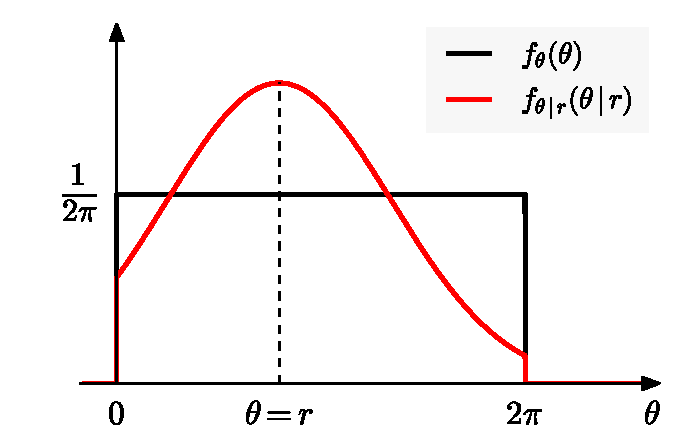
\includegraphics[width=\textwidth]{figuras/random_phase_posterior_probability.pdf}
  \end{minipage}\hfill
  \begin{minipage}[c]{0.5\textwidth}
    \caption{
       Densidad \(f_\theta(\theta)\) a priori y densidad \(f_{\theta\,|\,r}(\theta\,|\,r)\) a posteriori. La distribución a posteriori refleja el conocimiento brindado por la observación \(\mathbf{r}\). Luego de conocido \(\mathbf{r}\), la probabilidad de \(\theta\) ya no es uniforme, sino que tiene valores mas probables en torno a \(r\).
    } \label{fig:random_phase_posterior_probability}
  \end{minipage}
\end{figure}

\section{Valores esperados condicionales}

Aplicando la ecuación \ref{eq:mean_of_gx} a densidades condicionales, se observa que la esperanza de \(g(\y)\) es
\begin{equation}\label{eq:conditional_mean_of_g_definition}
 E\{g(\y)\,|\,M\}=\int_{-\infty}^{\infty}g(y)f(y\,|\,M)\,dy.
\end{equation}
Además, si \(M=\{x<\x\leq x+\Delta x\}\) con \(\Delta x\to 0\) se obtiene que 
\[
 E\{g(\y)\,|\,x\}=\int_{-\infty}^{\infty}g(y)f(y\,|\,x)\,dy.
\]
En particular, la \emph{media condicional} de \(\y\) dado que \(\x=x\) es 
\begin{equation}\label{eq:conditional_mean_definition}
 \eta_{y|x}=E\{\y\,|\,x\}=\int_{-\infty}^{\infty}yf(y\,|\,x)\,dy,
\end{equation}
y la \emph{varianza condicional} es
\[
 \sigma^2_{y|x}=E\{(\y-\eta_{y|x})^2\,|\,x\}=\int_{-\infty}^{\infty}(y-\eta_{y|x})^2f(y\,|\,x)\,dy.
\]

\paragraph{Ejemplo (6-48)} Sea
\[
 f_{xy}(x,\,y)
 =\left\{\begin{array}{ll}
   1 & 0<|y|<x<1\\ 
   0, & \textrm{en otro caso}
 \end{array} \right..
\]
Se quiere determinar \(E\{\x\,|\,y\}\) y \(E\{\y\,|\,x\}\).

Como se muestra en la figura \ref{fig:conditional_means_example}, \(f_{xy}(x,\,y)=1\) en la región sombreada y 0 en el resto del plano. Por lo tanto, el marginal de \(\x\) es
\[
 f_x(x)=\int_{-\infty}^{\infty}f_{xy}(x,\,y)\,dy = \int_{-x}^{x}1\cdot\,dy=2x,\qquad 0<x<1
\]
y la densidad marginal de \(\y\) es
\[
 f_y(y)=\int_{-\infty}^{\infty}f_{xy}(x,\,y)\,dx = \int_{|y|}^{1}1\cdot\,dx=1-|y|,\qquad |y|<1.
\]
De esta forma, a partir de las ecuaciones \ref{eq:conditional_joint_densities}, se tiene que
\[
 f_{x|y}(x\,|\,y)=\frac{f_{xy}(x,\,y)}{f_y(y)}=\frac{1}{1-|y|},\qquad 0<|y|<x<1
\]
y
\[
 f_{y|x}(y\,|\,x)=\frac{f_{xy}(x,\,y)}{f(y)}=\frac{1}{2x},\qquad 0<|y|<x<1.
\]
\begin{figure}[!htb]
  \begin{minipage}[c]{0.4\textwidth}
    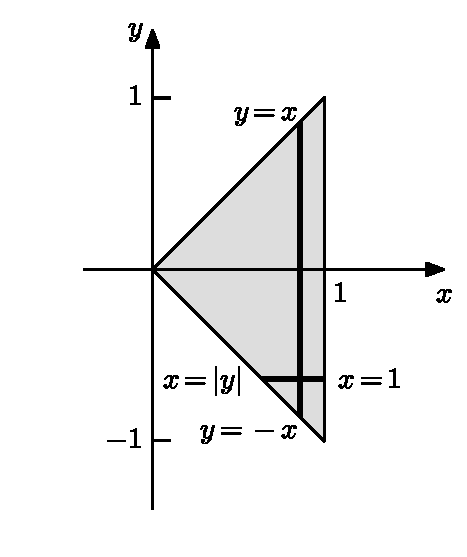
\includegraphics[width=\textwidth]{figuras/conditional_means_example.pdf}
  \end{minipage}\hfill
  \begin{minipage}[c]{0.57\textwidth}
    \caption{
       Densidad de probabilidad conjunta \(f_{xy}(x,\,y)\).
    } \label{fig:conditional_means_example}
  \end{minipage}
\end{figure}
Por lo tanto,
\begin{align*}
 E\{\x\,|\,y\}&=\int_{-\infty}^{\infty}xf_{x|y}(x\,|\,y)\,dx\\
   &=\int_{|y|}^{1}\frac{x}{1-|y|}\,dx\\
   &=\frac{1}{1-|y|}\cdot\frac{x^2}{2}\bigg|_{|y|}^{1}\\
   &=\frac{1-|y|^2}{2(1-|y|)}\\
   &=\frac{(1+|y|)(1-|y|)}{2(1-|y|)}\\
   &=\frac{1+|y|}{2},\qquad |y|<1,
\end{align*}
y
\begin{align*}
 E\{\y\,|\,x\}&=\int_{-\infty}^{\infty}yf_{y|x}(y\,|\,x)\,dy\\
   &=\int_{-x}^{x}\frac{y}{2x}\,dy\\
   &=\frac{1}{2x}\cdot\frac{y^2}{2}\bigg|_{-x}^{x}\\
   &=\frac{x^2-(-x)^2}{4x}\\
   &=0,\qquad 0<x<1,
\end{align*}


Para un \(x\) dado, la integral de la ecuación \ref{eq:conditional_mean_definition} es el centro de gravedad de la masa en la banda vertical \((x,\,x+dx)\). El lugar de esos puntos al variar \(x\) es la función
\begin{equation}\label{eq:linear_regression}
 \varphi(x)=\int_{-\infty}^{\infty}yf(y\,|\,x)\,dy,
\end{equation}
denominada \emph{línea de regresión}.

A partir de los resultados de las ecuaciones \ref{eq:mean_of_gxy} y \ref{eq:conditional_mean_of_g_definition} se deduce que
\begin{equation}\label{eq:conditional_mean_of_gxy_definition}
 E\{g(\x,\,\y)\,|\,M\}=\int_{-\infty}^{\infty}\int_{-\infty}^{\infty}g(x,\,y)f(x,\,y\,|\,M)\,dx\,dy.
\end{equation}
Para definir \(E\{g(\x,\,\y)\,|\,x\}\), hay que considerar límites. Estableciendo \(x_1=x\) y \(x_2=x+\Delta x\) en la ecuación \ref{eq:conditional_joint_density_aux}, se tiene que
\[
 f(x,\,y\,|\,x<\x\leq x+\Delta x)
 =\left\{\begin{array}{ll}
   \dfrac{f(x,\,y)}{F_x(x+\Delta x)-F_x(x)}, & x<x\leq x+\Delta x\\ 
   0, & \textrm{en otro caso}
 \end{array} \right.
\]
y sustituyendo en la ecuación \ref{eq:conditional_mean_of_gxy_definition} con \(M=\{x<\x\leq x+\Delta x\}\) se tiene que
\[
 E\{g(\x,\,\y)\,|\,x<\x\leq x+\Delta x\}=\int_{-\infty}^{\infty}\int_{x}^{x+\Delta x}\frac{g(\alpha,\,y)f(\alpha,\,y)}{F_x(\alpha+\Delta x)-F_x(\alpha)}\,d\alpha\,dy.
\]
Con \(\Delta x\to 0\), la integral interior tiende a \(g(x,\,y)f(x,\,y)/f(x)\). Definiendo \\ \(E\{g(\x,\,\y)\,|\,x\}\) como el límite de la integral, se concluye que
\[
  E\{g(\x,\,\y)\,|\,x\}=\int_{-\infty}^{\infty}g(x,\,y)f(y\,|\,x)\,dy,
\]
donde se usó que \(f(y\,|\,x)=f(x,\,y)/f(x)\). Notar que también se cumple que
\[
 E\{g(x,\,\y)\,|\,x\}=\int_{-\infty}^{\infty}g(x,\,y)f(y\,|\,x)\,dy,
\]
ya que \(g(x,\,\y)\) es una función de la variable aleatoria \(\y\) con un parámetro \(x\) y por lo tanto se aplica la ecuación \ref{eq:conditional_mean_of_g_definition}. Por lo tanto,
\[
 E\{g(\x,\,\y)\,|\,x\}=E\{g(x,\,\y)\,|\,x\}.
\]

\subsection{Valores esperados condicionados a variables aleatorias}\label{sec:conditional_expected_values_as_rv}

La media condicional de \(\y\) dado \(\x=x\) es una función \(\varphi(x)=E\{\y|x\}\) de \(x\) dada por la ecuación \ref{eq:linear_regression}. Usando esta función, se puede construir la variable aleatoria \(\varphi(\x)=E\{\y\,|\,\x\}\), y como indica la ecuación \ref{eq:mean_of_gx}, la media es
\[
 E\{\varphi(\x)\}=\int_{-\infty}^{\infty}f(x)\int_{-\infty}^{\infty}yf(y\,|\,x)\,dy\,dx.
\]
Considerando que \(f(x,\,y)=f(x)f(y\,|\,x)\), se obtiene que
\begin{align*}
 E\{E\{\y\,|\,\x\}\}&=\int_{-\infty}^{\infty}\int_{-\infty}^{\infty}yf(x,\,y)\,dx\,dy\\
   &=\int_{-\infty}^{\infty}y\left[\int_{-\infty}^{\infty}f(x,\,y)\,dx\right]\,dy\\
   &=\int_{-\infty}^{\infty}yf_y(y)\,dy\\
   &=E\{\y\}.
\end{align*}
Este resultado puede generalizarse. La media condicional \(E\{g(\x,\,\y)\,|\,x\}\) de \(g(\x,\,\y)\) dado \(\x=x\) es una función de la variable real \(x\). A partir de esta función, puede definirse una nueva variable aleatoria \(E\{g(\x,\,\y)\,|\,\x\}\),
\[
 E\{g(\x,\,\y)\,|\,\x\}=\int_{-\infty}^{\infty}g(\x,\,y)f(y\,|\,\x)\,dy.
\]
La media de esta variable aleatoria es
\begin{align*}
 E\{E\{g(\x,\,\y)\,|\,\x\}\}&=\int_{-\infty}^{\infty}f(x)\int_{-\infty}^{\infty}g(x,\,y)f(y\,|\,x)\,dy\,dx\\
   &=\int_{-\infty}^{\infty}\int_{-\infty}^{\infty}g(x,\,y)f(x,\,y)\,dx\,dy\\
   &=E\{g(\x,\,\y)\},
\end{align*}
es decir
\[
 E\{E\{g(\x,\,\y)\,|\,\x\}\}=E\{g(\x,\,\y)\}.
\]
Finalmente, se observa que
\[
 E\{g_1(\x)g_2(\y)\,|\,x\}=E\{g_1(x)g_2(\y)\,|\,x\}=g_1(x)E\{g_2(\y)\,|\,x\}
\]
\[
 E\{g_1(\x)g_2(\y)\}=E\{E\{g_1(\x)g_2(\y)\,|\,\x\}\}=E\{g_1(\x)E\{g_2(\y)\,|\,\x\}\}
\]
La última igualdad de la segunda ecuación se puede comprobar expresando la esperanza explícitamente como una integral,
\begin{align*}
 E\{g_1(\x)E\{g_2(\y)\,|\,\x\}\}&=\int_{-\infty}^{\infty}g_1(x)\left[\int_{-\infty}^{\infty}g_2(y)f(y\,|\,x)\,dy\right]f(x)\,dx\\
  &=\int_{-\infty}^{\infty}\int_{-\infty}^{\infty}g_1(x)g_2(y)f(x,\,y)\,dx\,dy\\
  &=E\{g_1(\x)g_2(\y)\}.
\end{align*}

\paragraph{Ejemplo (6-50)}

Sean las variables aleatorias \(\x\) e \(\y\) conjuntamente normales de distribución \(N(0,\,0,\,\sigma_1^2,\,\sigma_2^2,\,r)\). Se quiere mostrar que se cumple que
\[
 E\{\x\y\}=r\sigma_1\sigma_2,\qquad E\{\x^2\y^2\}=E\{\x^2\}E\{\y^2\}+2E^2\{\x\y\}.
\]

Se parte teniendo en cuenta que (ver ecuación \ref{eq:gaussian_rv_moments})
\[
 E\{\x^2\}=\sigma_1^2,\qquad E\{\x^2\}=2\sigma_1^4.
\]
Además, como indica la ecuación \ref{eq:joint_normal_conditional_pdf}, \(f(y\,|\,x)\) es normal con media \(r\sigma_2x/\sigma_1\) y varianza \(\sigma_2^2(1-r^2)\). Por lo tanto, de la ecuación \ref{eq:normal_rv_moments} se tiene que
\[
 E\{\y^2\,|\,x\}=\eta_{y|x}^2+\sigma_{y|x}^2=\left(\frac{r\sigma_2x}{\sigma_1}\right)^2+\sigma_2^2(1-r^2).
\]
Para probar la primera identidad, se observa que
\begin{align*}
 E\{\x\y\}&=E\{E\{\x\y\,|\,\x\}\}=E\{\x E\{\y\,|\,\x\}\}=E\left\{\x\frac{r\sigma_2\x}{\sigma_1}\right\}\\
  &=\frac{r\sigma_2}{\sigma_1}E\left\{\x^2\right\}=\frac{r\sigma_2}{\sigma_1}\sigma_1^2
  =r\sigma_1\sigma_2.
\end{align*}
Para probar la segunda identidad, se ve que
\begin{align*}
 E\{\x^2\y^2\}&=E\{E\{\x^2\y^2\,|\,\x\}\}=E\{\x^2 E\{\y^2\,|\,\x\}\}\\
  &=E\left\{\x^2\left[\frac{r^2\sigma_2^2\x^2}{\sigma_1^2}+\sigma_2^2(1-r^2)\right]\right\}\\
  &=\frac{r^2\sigma_2^2}{\sigma_1^2}E\{\x^4\}+\sigma_2^2(1-r^2)E\{\x^2\}\\
  &=\frac{r^2\sigma_2^2}{\sigma_1^2}(3\sigma_1^4)+\sigma_2^2(1-r^2)(\sigma_1^2)\\
  &=3r^2\sigma_1^2\sigma_2^2+\sigma_1^2\sigma_2^2-r^2\sigma_1^2\sigma_2^2\\
  &=\sigma_1^2\sigma_2^2+2r^2\sigma_1^2\sigma_2^2\\
  &=E\{\x^2\}E\{\y^2\}+2E^2\{\x\y\}.
\end{align*}
Este resultado ya se obtuvo previamente a partir de la función generadora de momentos (ecuación \ref{eq:moment22_rv_jointly_normal}) y también mediante el teorema de Price.

\chapter{Secuencias de variables aleatorias}

\section{Conceptos generales}

Un vector aleatorio es un vector
\[
 \X=[\x_1,\dots,\x_n]
\]
cuyos componentes \(\x_i\) son variables aleatorias. La probabilidad de que \(\X\) pertenezca a una región \(D\) del espacio \(n\)-dimensional es
\[
 P\{\X\in D\}=\int_Df(X)dX,\qquad X=[x_1,\dots, x_n]
\]
donde 
\[
 f(X)=f(x_1,\dots,x_n)=\frac{\partial^nF(x_1,\dots,x_n)}{\partial x_1\dots\partial x_n}
\]
es la densidad de probabilidad conjunta (o multivariada) de las variables aleatorias \(\x_i\) y 
\[
 F(X)=F(x_1,\dots,x_n)=P\{\x_1\leq x_1,\dots,\x_n\leq x_n\}
\]
es la distribución de probabilidad conjunta.

Generalizando los resultados de la sección \ref{sec:marginal_statisctics_two_rv}, si en \(F(x_1,\dots,x_n)\) se sustituyen ciertas variables por \(\infty\), se obtiene la distribución de las variables restantes. Si se integra \(f(x_1,\dots,x_n)\) respecto a ciertas variables, se obtiene la densidad de las variables restantes. Como ejemplo, se cumple que
\begin{equation}\label{eq:marginal_statisctics_sequence_rv}
 \begin{aligned}
 F(x_1,\,x_3)&=F(x_1,\,\infty,\,x_3,\,\infty)\\
 f(x_1,\,x_3)&=\int_{-\infty}^{\infty}\int_{-\infty}^{\infty}f(x_1,\,x_2,\,x_3,\,x_4)\,dx_2\,dx_4
 \end{aligned}
\end{equation}

\paragraph{Transformaciones} Dadas \(k\) funciones 
\[
 g_1(X),\dots,g_k(X),\qquad X=[x_1,\dots,x_n]
\]
se construyen las \(k\) variables aleatorias
\[
 \y_1=g_1(\X),\dots,\y_k=g_k(\X).
\]
La estadística de estas variables aleatorias puede determinarse en términos de la estadística de \(\X\), de forma análoga a lo explicado en la sección \ref{sec:two_funcions_of_two_rv}. Se considerará el caso en que \(k=n\), ya que los casos en que \(k<n\) o \(k>n\) pueden reducirse a \(k=n\), como se explica en el capítulo 7 de \cite{papoulis2002probability}. 

Para obtener la densidad \(f_y(y_1,\dots,y_n)\) del vector aleatorio \(\Y=[\y_1,\dots,\y_n]\) para un conjunto específico de valores \(y_1,\dots,y_n\), se resuelve el sistema
\begin{equation}\label{eq:rv_sequence_transformation}
 g_1(X)=y_1,\dots,g_n(X)=y_n.
\end{equation}
Si el sistema no tiene soluciones, \(f_y(y_1,\dots,y_n)=0\). Si el sistema tiene una solución única \(X=[x_1,\dots,x_n]\),
\begin{equation}\label{eq:rv_sequence_transformation_density}
 f_y(y_1,\dots,y_n)=\frac{f_x(x_1,\dots,x_n)}{|J(x_1,\dots,x_n)|}
\end{equation}
donde
\[
 J(x_1,\dots,x_n)=
 \begin{vmatrix}
    \dfrac{\partial g_1}{\partial x_1} & \cdots & \dfrac{\partial g_1}{\partial x_n} \\
    \hdotsfor{3} \\
    \dfrac{\partial g_n}{\partial x_1} & \cdots & \dfrac{\partial g_n}{\partial x_n}
\end{vmatrix}
\]
es la matriz jacobiana de la transformación \ref{eq:rv_sequence_transformation}. Si el sistema tiene múltiples soluciones, se suman los términos correspondientes como en la ecuación \ref{eq:joint_density_two_funcions_two_rv}.

\subsection{Independencia}

Se dice que las variables aleatorias \(\x_1,\dots,\x_n\) son mutuamente independientes si los eventos \(\{\x_1\leq x_1\},\dots,\{\x_n\leq x_n\}\) son independientes. En ese caso, se cumple que
\begin{align*}
  F_x(x_1,\dots,x_n)&=F(x_1)\dots F(x_n)\\
  f_x(x_1,\dots,x_n)&=f(x_1)\dots f(x_n).
\end{align*}
Una observación respecto a la notación, es que las funciones se están identificando a través del nombre de la variable. Las funciones \(f(x_i)\) en la ecuación anterior no necesariamente son iguales, sino que la densidad \(f_i(x_i)\) de la variable aleatoria \(\x_i\) se denotó \(f(x_i)\).  

\paragraph{Ejemplo (7-1)} Sean \(n\) variables aleatorias \(\x_i\) con respectivas densidades de probabilidad \(f_i(x_i)\). Se construyen las variables aleatorias
\[
 \y_k=\x_1+\dots+\x_k,\qquad k=1,\dots,\,n.
\]
Se quiere determinar la densidad de probabilidad conjunta de \(\y_k\).

La solución del sistema
\begin{equation}\label{eq:rv_sequence_transformation_example_gx}
 \begin{aligned}
 x_1&=y_1=g_1(X)\\
 x_1+x_2&=y_2=g_2(X)\\
 &\;\;\vdots\\
 x_1+\dots+x_n&=y_n=g_n(X)
\end{aligned}
\end{equation}
es
\begin{align*}
 x_1&=y_1\\
 x_2&=y_2-x_1=y_2-y_1\\
 x_3&=y_3-(x_1+x_2)=y_3-y_2\\
 &\;\;\vdots\\
 x_n&=y_n-(x_1+\dots+x_{n-1})=y_n-y_{n-1},
\end{align*}
es decir,
\[
 x_k=y_k-y_{k-1},\qquad 1\leq k\leq n.
\]
A partir de \ref{eq:rv_sequence_transformation_example_gx} se obtiene que el valor absoluto del determinante de la matriz jacobiana es
\[
 |J(x_1,\dots,x_n)|=
 \begin{vmatrix}
    1 & 0 & 0 & 0 & \cdots & 0\\
    1 & 1 & 0 & 0 & \cdots & 0\\
    1 & 1 & 1 & 0 & \cdots & 0\\
    \vdots & \vdots & \vdots &  \ddots & \ddots & \vdots\\
    1 & 1 & 1 & \cdots & 1 & 0\\
    1 & 1 & 1 & \cdots & 1 & 1\\
\end{vmatrix}
=1.
\]
Además, teniendo en cuenta que las variables aleatorias \(\x_i\) son independientes y por lo tanto se cumple que
\[
 f_x(x_1,\dots,x_n)=f_1(x_1)\dots f_n(x_n),
\]
aplicando la ecuación \ref{eq:rv_sequence_transformation_density} se obtiene que
\[
 f_y(y_1,\dots,y_n)=f_1(y_1)f_2(y_2-y_1)\cdots f_n(y_n-y_{n-1}).
\]

\subsection{Experimentos independientes y ensayos repetidos}

Considérese el experimento combinado
\[
 S^n=S_1\times\cdots\times S_n
\]
donde las variables aleatorias \(\x_i\) dependen únicamente de las salidas \(\zeta_i\) de \(S_i\), es decir
\[
 \x_i(\zeta_1\cdots\zeta_i\cdots\zeta_n)=\x_i(\zeta_i),\qquad i=1,\dots,n.
\]
Si los experimentos \(S_i\) son independientes, las variables aleatorias \(\x_i\) son independientes.

Como caso particular de interés, supóngase que \(\x\) es una variable aleatoria definida en un experimento \(S\), y el experimento se repite \(n\) veces generando el experimento \(S^n=S\times\cdots\times S\). En este experimento se definen las variables aleatorias \(\x_i\) tal que
\begin{equation}\label{eq:rv_sequence_repeated_trials}
 \x_i(\zeta_1\cdots\zeta_i\cdots\zeta_n)=\x(\zeta_i),\qquad i=1,\dots,n.
\end{equation}
Por lo tanto, la distribución \(F_i(x_i)\) de \(\x_i\) es \(F(x)\), la distribución de la variable aleatoria \(\x\). Como conclusión, si un experimento se repite \(n\) veces, las variables aleatorias \(\x_i\) definidas como en \ref{eq:rv_sequence_repeated_trials} son independientes y tienen la misma distribución \(F_x(x)\). Estas variables aleatorias se denominan \emph{i.i.d.} (independientes e idénticamente distribuidas).

\paragraph{Estadísticos de orden}

Los estadísticos de orden de las variables aleatorias \(\x_i\) son \(n\) variables aleatorias \(\y_k\) definidas de la siguiente forma: para determinada salida \(\zeta\), las variables aleatorias \(\x_i\) tomas valores \(\x_i(\zeta)\). Ordenando esos valores de forma creciente, se obtiene la secuencia
\[
 \x_{r_1}(\zeta)\leq\cdots\leq\x_{r_k}(\zeta)\leq\cdots\leq\x_{r_n}(\zeta) 
\]
y se define la variable aleatoria \(\y_k\) tal que
\[
 \y_1=\x_{r_1}(\zeta)\leq\cdots\leq\y_k=\x_{r_k}(\zeta)\leq\cdots\leq\y_n=\x_{r_n}(\zeta).
\]
Se demostrará que la densidad \(f_k(y)\) del \(k\)-ésimo estadístico \(\y_k\) es
\begin{equation}\label{eq:ordered_statistic_density}
 f_k(y)=\frac{n!}{(k-1)!(n-k)!}F_x^{k-1}(y)[1-F_x(y)]^{n-k}f_x(y).
\end{equation}
donde \(F_x(x)\) y \(f_x(x)\) son la distribución y la densidad de las variables aleatorias i.i.d. \(\x_i\).

Para demostrarlo, se parte observando que el evento \(B=\{y<\y_k\leq y+dy\}\) ocurre si exactamente \(k-1\) variables aleatorias \(\x_i\) toman un valor menor a \(y\) y una toma un valor en el intervalo \((y,\,y+dy)\).
Además, se cumple que 
\[
 f_k(y)dy=P\{y<\y_k\leq y+dy\}.
\]

En el experimento original \(S\), los eventos
\[
 A_1=\{\x\leq y\}\qquad A_2=\{y<\x\leq y+dy\}\qquad A_3=\{\x>y+dy\}
\]
forman una partición y
\[
 P(A_1)=F_x(y)\qquad P(A_2)=f_x(y)dy\qquad P(A_3)=1-F_x(y).
\]
En el experimento \(S^n\), el evento \(B\) ocurre si \(A_1\) ocurre \(k-1\) veces, \(A_2\) ocurre una vez y \(A_3\) ocurre \(n-k\) veces. Sustituyendo estos resultados en la ecuación \ref{eq:bernoulli_trials_generalization} se llega al resultado que se quería demostrar.

Notar en particular que
\[
 f_1(y)=n[1-F_x(y)]^{n-1}f_x(y),\qquad f_n(y)=nF_x^{n-1}(y)f_x(y).
\]

Como ejemplo, considérese el caso en que las variables aleatorias \(\x_i\) son uniformes en \((0,\,\theta)\). En ese caso,
\[
 f_x(x)
 =\left\{\begin{array}{ll}
   1/\theta, & 0<x<\theta\\ 
   0, & \textrm{en otro caso}
 \end{array} \right.,
 \qquad
 F_x(x)
 =\left\{\begin{array}{ll}
   0, & x<0\\
   x/\theta, & 0<x<\theta\\ 
   1, & x>\theta
 \end{array} \right..
\]
En este caso, usando la ecuación \ref{eq:ordered_statistic_density} se concluye que
\begin{equation}\label{eq:ordered_statistic_uniform_density}
  f_1(y)=\frac{n}{\theta}\left(1-\frac{y}{\theta}\right)^{n-1},\qquad f_n(y)=\frac{ny^{n-1}}{\theta^n}. 
\end{equation}
Estos resultados son la densidad de probabilidad del mínimo y el máximo respectivamente de \(n\) variables aleatorias i.i.d. uniformes.

\subsection{Media y covarianza}

Extendiendo la ecuación \ref{eq:mean_of_gxy} para \(n\) variables aleatorias, se concluye que la media de \(g(\x_1,\dots,\x_n)\) es
\[
 E\{g(\x_1,\dots,\x_n)\}=\int_{-\infty}^{-\infty}\cdots\int_{-\infty}^{-\infty}g(x_1,\dots,x_n)f(x_1,\dots,x_n)\,dx_1\dots dx_n.
\]
En el caso en que las variables aleatorias \(\z_i=\x_i+j\y_j\) son complejas, la media de \(g(\z_1,\dots,\z_n)\) es
\[
 \int_{-\infty}^{-\infty}\cdots\int_{-\infty}^{-\infty}g(z_1,\dots,z_n)f(x_1,\dots,x_n,\,y_1,\dots,y_n)\,dx_1\dots dx_ndy_1\dots dy_n.
\]

A partir de estas consideraciones, se deduce que la media es lineal, 
\[
 E\{a_1g_1(\X)+\cdots+a_ng_n(\X)\}=a_1E\{g_1(\X)\}+\cdots+a_nE\{g_n(\X)\},
\]
para cualquier vector \(\X\) real o complejo.

\paragraph{Correlación y covarianza}

La covarianza de dos variables aleatorias reales está definida por la ecuación \ref{eq:covariance_definition}. La covarianza \(C_{ij}\) entre dos variables aleatorias complejas \(\x_i\) y \(\x_j\) se define como
\[
 C_{ij}=E\{(\x_i-\eta_i)(\x^*_j-\eta^*_j)\}=E\{\x_i\x^*_j\}-E\{\x_i\}E\{\x^*_j\},
\]
y la varianza de la variable aleatoria compleja \(\x_i\) se define como
\[
 \sigma_i^2=C_{ii}=E\{(\x_i-\eta_i)(\x^*_i-\eta^*_i)\}=E\{|\x_i-\eta_i|^2\}=E\{|\x_i|^2\}-|E\{\x_i\}|^2.
\]
Se dice que las variables aleatorias \(\x_i\) son \emph{no correlacionadas} si \(C_{ij}=0\) para todo \(i\neq j\). En ese caso se cumple que si
\begin{equation}\label{eq:variance_sum_of_uncorrelated_rv}
 \x=\x_1+\cdots+\x_n,\qquad\textrm{entonces}\qquad\sigma_x^2=\sigma_1^2+\cdots+\sigma_n^2,
\end{equation}
como se mencionó en la sección \ref{sec:uncorrelation_and_onthogonality}.

\paragraph{Ejemplo 7-5: media y varianza muestral}\label{sec:sample_mean_and_variance}

La \emph{media muestral} y la \emph{varianza muestral} de las variables aleatorias \(\x_i\) se definen como las variables aleatorias
\begin{equation}\label{eq:sample_mean_and_variance}
 \bar{\x}=\frac{1}{n}\sum_{i=1}^{n}\x_i, \qquad \bar{\mathbf{v}}=\frac{1}{n-1}\sum_{i=1}^{n}(\x_i-\bar{\x})^2
\end{equation}
respectivamente. Se demostrará que si las variables aleatorias \(\x_i\) son no correlacionadas, todas con media \(E\{\x_i\}=\eta\) y varianza \(\sigma_i^2=\sigma^2\), la media y la varianza de la media muestral es
\[
 E\{\bar{\x}\}=\eta,\qquad \sigma_{\bar{x}}^2=\frac{\sigma^2}{n}
\]
y la media y la varianza de la varianza muestral es
\[
 E\{\bar{\mathbf{v}}\}=\sigma^2,\qquad \sigma^2_{\bar{v}}=\frac{1}{n}\left(\mu_4-\frac{n-3}{n-1}\sigma^4\right).
\]

La media de la media muestral se obtiene directamente a partir de la linealidad de la esperanza,
\[
 E\{\bar{\x}\}=E\left\{\frac{1}{n}\sum_{i=1}^{n}\x_i\right\}=\frac{1}{n}\sum_{i=1}^{n}E\{\x_i\}=\frac{1}{n}\sum_{i=1}^{n}\eta=\frac{1}{n}(n\eta)=\eta.
\]
Para obtener la varianza, se observa que para cualquier constante \(a\) se cumple que
\begin{align*}
 \sigma_{ax}^2&\overset{(a)}{=}E\{(a\x-E\{a\x\})^2\}\\
   &\overset{(b)}{=}E\{(a\x-aE\{\x\})^2\}\\
   &=E\{a^2(\x-E\{\x\})^2\}\\
   &\overset{(c)}{=}a^2E\{(\x-E\{\x\})^2\}\\
   &=a^2\sigma_x^2,
\end{align*}
donde en \((a)\) se usó la definición de varianza (ecuación \ref{eq:variance_definition1}) y en \((b)\) y \((c)\) la propiedad de linealidad de la esperanza.
Combinando este resultado con el de la ecuación \ref{eq:variance_sum_of_uncorrelated_rv}, se tiene que
\[
 \sigma_{\bar{x}}^2=\frac{1}{n^2}\sum_{i=1}^{n}\sigma_i^2=\frac{1}{n^2}\sum_{i=1}^{n}\sigma^2=\frac{1}{n^2}(n\sigma^2)=\frac{\sigma^2}{n}.
\]
A continuación se obtendrá  el mismo resultado sin emplear las propiedades de la varianza. Partiendo de la definición de varianza de la ecuación \ref{eq:variance_definition2}, se observa que
\begin{align}\label{eq:sample_mean_variance_aux}
 \sigma_{\bar{x}}^2&=E\{\bar{\x}^2\}-E^2\{\bar{\x}\}\nonumber\\
   &\overset{(a)}{=}E\left\{\left(\frac{1}{n}\sum_{i=1}^{n}\x_i\right)^2\right\}-\eta^2\nonumber\\
   &=\frac{1}{n^2}E\left\{\left(\sum_{i=1}^{n}\x_i\right)^2\right\}-\eta^2,
\end{align}
donde en \((a)\) se empleó que \(E\{\bar{\x}\}=\eta\), resultado obtenido antes. Observando que
\[
 \left(\sum_{i=1}^{n}\x_i\right)^2=\sum_{i=1}^{n}\x_i^2+\mathop{\sum_{i=1}^n\sum_{j=1}^n}_{i\neq j}\x_i\x_j
\]
se tiene que
\begin{align*}
 E\left\{\left(\sum_{i=1}^{n}\x_i\right)^2\right\}&\overset{(a)}{=}\sum_{i=1}^{n}E\{\x_i^2\}+\mathop{\sum_{i=1}^n\sum_{j=1}^n}_{i\neq j}E\{\x_i\x_j\}\\
  &\overset{(b)}{=}\sum_{i=1}^{n}E\{\x_i^2\}+\mathop{\sum_{i=1}^n\sum_{j=1}^n}_{i\neq j}E\{\x_i\}E\{\x_j\}\\
  &\overset{(c)}{=}\sum_{i=1}^{n}(\sigma^2+\eta^2)+\mathop{\sum_{i=1}^n\sum_{j=1}^n}_{i\neq j}\eta^2\\
  &\overset{(d)}{=}n(\sigma^2+\eta^2)+n(n-1)\eta^2\\
  &=n\sigma^2+n^2\eta^2,
\end{align*}
donde en \((a)\) se empleó la linealidad de la esperanza, en \((b)\) que las variables \(\x_i\) son no correlacionadas y por lo tanto \(E\{\x_i\x_j\}=E\{\x_i\}E\{\x_j\}\), en \((c)\) el resultado de la ecuación \ref{eq:moments_as_function_of_central_moments_first_4} y que todas las variables aleatorias \(\x_i\) tienen la misma media y varianza, y en \((d)\)  que la primer sumatoria tiene \(n\) sumandos y la segunda doble sumatoria tiene \(n(n-1)\) sumandos. Sustituyendo este resultado en la ecuación \ref{eq:sample_mean_variance_aux}, se obtiene que
\[
 \sigma_{\bar{x}}^2=\frac{n\sigma^2+n^2\eta^2}{n^2}-\eta^2=\frac{\sigma^2}{n},
\]
que es lo que se quería demostrar.

Para calcular la media de la varianza muestral, 
\[
 E\{\bar{\mathbf{v}}\}=\frac{1}{n-1}\sum_{i=1}^{n}E\{(\x_i-\bar{\x})^2\}
\]
se observa que
\begin{align*}
 E\{(\x_i-\bar{\x})^2\}&=E\{[(\x_i-\eta)-(\bar{\x}-\eta)]^2\}\\
  &=E\{(\x_i-\eta)^2+(\bar{\x}-\eta)^2-2(\x_i-\eta)(\bar{\x}-\eta)\}\\
  &=E\{(\x_i-\eta)^2\}+E\{(\bar{\x}-\eta)^2\}-2E\{(\x_i-\eta)(\bar{\x}-\eta)\}
\end{align*}
El primer sumando en la última ecuación es \(\sigma^2\) y el segundo es \(\sigma^2_{\bar{x}}=\sigma^2/n\), calculado antes. El tercer sumando es
\begin{align*}
 E\{(\x_i-\eta)(\bar{\x}-\eta)\}&=E\left\{(\x_i-\eta)\left(\frac{1}{n}\sum_{j=1}^{n}\x_j-\eta\right)\right\}\\
   &=\frac{1}{n}E\left\{(\x_i-\eta)\sum_{j=1}^{n}\left(\x_j-\eta\right)\right\}\\
   &=\frac{1}{n}\sum_{j=1}^{n}E\left\{(\x_i-\eta)\left(\x_j-\eta\right)\right\}\\
   &\overset{(a)}{=}\frac{1}{n}E\left\{(\x_i-\eta)\left(\x_i-\eta\right)\right\}\\
   &=\frac{\sigma^2}{n},
\end{align*}
donde en \((a)\) se empleó que las variables \(\x_i\) son no correlacionadas por hipótesis y por lo tanto \(E\{(\x_i-\eta)(\x_j-\eta)\}=0\) si \(i\neq j\).
Por lo tanto,
\[
 E\{(\x_i-\bar{\x})^2\}=\sigma^2+\frac{\sigma^2}{n}-2\frac{\sigma^2}{n}=\frac{n-1}{n}\sigma^2.
\]
Finalmente,
\[
 E\{\bar{\mathbf{v}}\}=\frac{1}{n-1}\sum_{i=1}^{n}E\{(\x_i-\bar{\x})^2\}=\frac{1}{n-1}\sum_{i=1}^{n}\frac{n-1}{n}\sigma^2=\frac{n}{n-1}\frac{n-1}{n}\sigma^2=\sigma^2.
\]

Si las variables aleatorias \(\x_i\) son independientes e idénticamente distribuidas con momento central cuarto \(\mu_4=E\{|\x_i-\eta|^4\}\), se cumple que la varianza de la varianza muestral es
\begin{equation}\label{eq:sample_variance_variance}
 \sigma^2_{\bar{v}}=\frac{1}{n}\left(\mu_4-\frac{n-3}{n-1}\sigma^4\right).
\end{equation}
La demostración de esto es considerablemente tediosa y en \cite{papoulis2002probability} está como ejercicio. La demostración desarrollada aquí está basada en \cite{73080}\footnote{Otra demostración similar puede encontrarse en \url{http://mathworld.wolfram.com/SampleVarianceDistribution.html},}. Se comenzará mostrando que la varianza muestral puede escribirse de las siguientes formas alternativas,
\[
 \bar{\mathbf{v}}=\frac{1}{n-1}\left(\sum_{i=1}^{n}\x_i^2-n\bar{\x}^2\right),\qquad
 \bar{\mathbf{v}}=\frac{1}{n(n-1)}\sum_{i=1}^n\sum_{j=1}^n\frac{(\x_i-\x_j)^2}{2}.
\]
Partiendo de la definición de la varianza muestral, para mostrar la primer identidad se ve que
\begin{align*}
 \bar{\mathbf{v}}&=\frac{1}{n-1}\sum_{i=1}^{n}(\x_i-\bar{\x})^2\\
   &=\frac{1}{n-1}\sum_{i=1}^{n}(\x_i^2+\bar{\x}^2-2\x_i\bar{\x})\\
   &=\frac{1}{n-1}\left(\sum_{i=1}^{n}\x_i^2+\sum_{i=1}^{n}\bar{\x}^2-2\bar{\x}\sum_{i=1}^{n}\x_i\right)\\
   &=\frac{1}{n-1}\left(\sum_{i=1}^{n}\x_i^2+n\bar{\x}^2-2\bar{\x}(n\bar{\x})\right)\\
   &=\frac{1}{n-1}\left(\sum_{i=1}^{n}\x_i^2-n\bar{\x}^2\right).
\end{align*}

Para demostrar la segunda identidad, se desarrolla el lado derecho de la siguiente forma,
\begin{align*}
 \frac{1}{n(n-1)}\sum_{i,\,j}\frac{(\x_i-\x_j)^2}{2}&=\frac{1}{2n(n-1)}\sum_{i,\,j}(\x_i^2+\x_j^2-2\x_i\x_j)\\
 &=\frac{1}{2n(n-1)}\left(\sum_{i,\,j}\x_i^2+\sum_{i,\,j}\x_j^2-2\sum_{i,\,j}\x_i\x_j\right)\\
 &=\frac{1}{2n(n-1)}\left(n\sum_{i=1}^n\x_i^2+n\sum_{j=1}^n\x_j^2-2\sum_{i=1}^n\x_i\sum_{j=1}^n\x_j\right)\\
 &=\frac{1}{2n(n-1)}\left[2n\sum_{i=1}^n\x_i^2-2\left(\sum_{i=1}^n\x_i\right)^2\right]\\
 &=\frac{1}{(n-1)}\left[\sum_{i=1}^n\x_i^2-\frac{1}{n}(n\bar{\x})^2\right]\\
 &=\frac{1}{(n-1)}\left(\sum_{i=1}^n\x_i^2-n\bar{\x}^2\right)=\bar{\mathbf{v}}.
\end{align*}
Para calcular la varianza \(\sigma_{\bar{v}}^2\) de la varianza muestral, se utilizará esta expresión de la varianza muestral. De la definición de varianza, se tiene que
\[
 \sigma_{\bar{v}}^2=E\{(\bar{\mathbf{v}}-E\{\bar{\mathbf{v}}\})^2\}.
\]
Teniendo en cuenta que \(E\{\bar{\mathbf{v}}\}=\sigma^2\), como se demostró previamente, hay que calcular
\begin{align}\label{eq:sample_variance_variance_tmp1}
 \sigma_{\bar{v}}^2&=E\left\{\left[\frac{1}{n(n-1)}\sum_{i,\,j}\frac{(\x_i-\x_j)^2}{2}-\sigma^2\right]\left[\frac{1}{n(n-1)}\sum_{k,\,l}\frac{(\x_k-\x_l)^2}{2}-\sigma^2\right]\right\}\nonumber\\
   &=E\left\{\frac{1}{n^2(n-1)^2}\sum_{i,\,j}\frac{(\x_i-\x_j)^2}{2}\sum_{k,\,l}\frac{(\x_k-\x_l)^2}{2}-\frac{2\sigma^2}{n(n-1)}\sum_{i,\,j}\frac{(\x_i-\x_j)^2}{2}+\sigma^4\right\}\nonumber\\
   &=\frac{1}{4n^2(n-1)^2}\sum_{i,\,j}\sum_{k,\,l}E\{(\x_i-\x_j)^2(\x_k-\x_l)^2\}-\frac{\sigma^2}{n(n-1)}\sum_{i,\,j}E\{(\x_i-\x_j)^2\}+\sigma^4.
\end{align}

Comenzando con el segundo sumando de esta expresión, se observa que
\begin{align*}
 E\{(\x_i-\x_j)^2\}&=E\{[(\x_i-\eta)-(\x_j-\eta)]^2\}\\
  &=E\{(\x_i-\eta)^2\}+E\{(\x_j-\eta)^2\}-2E\{(\x_i-\eta)(\x_j-\eta)\}\\
  &\overset{(a)}{=}2\sigma^2,
\end{align*}
donde en \((a)\) se consideró que \(\x_i\) y \(\x_j\) son independientes y por lo tanto \(C_{ij}=E\{(\x_i-\eta)(\x_j-\eta)=0\). Esta igualdad es válida si \(i\neq j\). Si \(i=j\), el resultado es 0. Además, la sumatoria en \((i,\, j)\) con \(i\neq j\) tiene \(n(n-1)\) sumandos. De esta forma, el segundo sumando de \ref{eq:sample_variance_variance_tmp1} es
\begin{equation}\label{eq:sample_variance_variance_tmp2}
 \frac{\sigma^2}{n(n-1)}\sum_{i,\,j}E\{(\x_i-\x_j)^2\}=\frac{\sigma^2}{n(n-1)}2\sigma^2n(n-1)=2\sigma^4.
\end{equation}

Para calcular el primer sumando de \ref{eq:sample_variance_variance_tmp1}, hay que calcular
\[
 E\{(\x_i-\x_j)^2(\x_k-\x_l)^2\}.
\] 
Claramente, esta expresión es nula si \(i=j\) o \(k=l\). Asimismo, toma valores distintos dependiendo del tamaño de \(\{i,\,j\}\cap\{k,\,l\}\), que puede ser 0, 1 o 2. Se discuten a continuación cada uno de estos casos.
\begin{enumerate}
 \item \(|\{i,\,j\}\cap\{k,\,l\}|=0\), es decir, \(i,\,j,\,k,\,l\) son todos distintos. Como las variables aleatorias son independientes, se cumple que
 \[
  E\{(\x_i-\x_j)^2(\x_k-\x_l)^2\}=E\{(\x_i-\x_j)^2\}E\{(\x_k-\x_l)^2\}=4\sigma^4,
 \]
donde en la última igualdad se empleó el resultado obtenido antes.
 \item \(|\{i,\,j\}\cap\{k,\,l\}|=1\), es decir, \(i\) o \(j\) es igual a \(k\) o \(l\). En este caso, hay que hacer todas las cuentas. Expandiendo el producto dentro de la esperanza, se tiene que
 \begin{align*}
  (\x_i^2+\x_j^2-2\x_i\x_j)(\x_k^2+\x_l^2-2\x_k\x_l)=&\,\x_i^2\x_k^2+\x_i^2\x_l^2+\x_j^2\x_k^2+\x_j^2\x_l^2\\
    &\,-2\x_i^2\x_k\x_l-2\x_j^2\x_k\x_l\\
    &\,-2\x_k^2\x_i\x_j-2\x_l^2\x_i\x_j\\
    &\,+4\x_i\x_j\x_k\x_l.
 \end{align*}
 Notar que esta expresión es simétrica en todas las variables y por lo tanto, en el caso en que \(|\{i,\,j\}\cap\{k,\,l\}|=1\), la expresión es equivalente sin importar el par de variables que sean iguales. Supóngase por ejemplo que \(k=i\) y \(j\neq l\). En ese caso,
 \begin{align*}
  (\x_i-\x_j)^2(\x_i-\x_l)^2=&\,\x_i^4+\x_i^2\x_l^2+\x_j^2\x_i^2+\x_j^2\x_l^2\\
    &-2\x_i^3\x_l-2\x_j^2\x_i\x_l-2\x_i^3\x_j-2\x_l^2\x_i\x_j\\
    &+4\x_i^2\x_j\x_l.
 \end{align*}
 Tomando esperanza y considerando que las variables aleatorias son independientes y que \(E\{\x_i^n\}=m_n\) es el momento \(n\)-ésimo de \(\x_i\), se tiene que
 \begin{align*}
  E\{(\x_i-\x_j)^2(\x_i-\x_l)^2\}&=m_4+3m_2m_2-4m_3m\\
   &\overset{(a)}{=}(\eta^4+6\sigma^2\eta^2+4\mu_3\eta+\mu_4)+3(\sigma^2+\eta^2)^2\\
   &\quad-4(\eta^3+3\sigma^2\eta+\mu_3)\eta\\
   &=(\eta^4+6\sigma^2\eta^2+4\mu_3\eta+\mu_4)\\
   &\quad+(3\sigma^4+3\eta^4+6\sigma^2\eta^2)\\
   &\quad-(4\eta^4+12\sigma^2\eta^2+4\mu_3\eta)\\
   &=\mu_4+3\sigma^4,
 \end{align*}
 donde en \((a)\) se usó la ecuación \ref{eq:moments_as_function_of_central_moments_first_4}, que expresa los momentos en función de los momentos centrales.
 \item \(|\{i,\,j\}\cap\{k,\,l\}|=2\), es decir, \(i=k\) y \(j=l\) o \(i=l\) y \(j=k\). En este caso, se tiene que
 \begin{align*}
  E\{(\x_i-\x_j)^4\}&=E\{\left[(\x_i-\eta)+(\x_j-\eta)\right]^4\}\\
    &=E\{(\x_i-\eta)^4\}+E\{(\x_j-\eta)^4\}\\
    &\quad-4E\{(\x_i-\eta)^3(\x_j-\eta)\}-4E\{(\x_i-\eta)(\x_j-\eta)^3\}\\
    &\quad+6E\{(\x_i-\eta)^2(\x_j-\eta)^2\}\\
    &\overset{(a)}{=}2\mu_4+6\sigma^4,
 \end{align*}
donde en \((a)\) se consideró que \(\x_i\) y \(\x_j\) son independientes y por lo tanto, la esperanza del producto es el producto de las esperanzas, y también que \(E\{\x_i-\eta\}=0\).
 \end{enumerate}
Estos son los tres tipos de sumandos distintos en la sumatoria cuádruple de índices \(i,\,j,\,k,\,l\), todos variando de 1 a \(n\) con \(i\neq j\) y \(k\neq l\). Por lo tanto, para obtener el resultado final, hay que contar la cantidad de sumandos que tienen \(|\{i,\,j\}\cap\{k,\,l\}|=0\), 1 y 2 en dicha sumatoria. Para hacerlo, notar que por ejemplo, si \(n=4\), la sumatoria se desarrolla como
\begin{align*}
 \bigl\{\left[(\x_1-\x_2)^2+(\x_1-\x_3)^2+(\x_1-\x_4)^2\right]&+\left[(\x_2-\x_1)^2+(\x_2-\x_3)^2+(\x_2-\x_4)^2\right]+\\
 \left[(\x_3-\x_1)^2+(\x_3-\x_2)^2+(\x_3-\x_4)^2\right]&+\left[(\x_4-\x_1)^2+(\x_4-\x_2)^2+(\x_4-\x_3)^2\right]\bigr\}^2.
\end{align*}
Se observa que hay \(n(n-1)\) términos de la forma \((\x_i-\x_j)^2\) entre las llaves, ya que hay \(n\) términos agrupados por corchetes, que se diferencian por el valor del primer índice, y \((n-1)\) términos \((\x_i-\x_j)^2\) dentro de los corchetes, diferenciados por el valor del segundo índice. Por lo tanto, al desarrollar el cuadrado se obtienen \(n^2(n-1)^2\) términos de la forma \((\x_i-\x_j)^2(\x_k-\x_l)^2\). A continuación se contarán la cantidad de términos con \(|\{i,\,j\}\cap\{k,\,l\}|=0\), 1 y 2.
\begin{enumerate}
 \item \(|\{i,\,j\}\cap\{k,\,l\}|=0\), es decir, todos los subíndices distintos.
 \begin{itemize}
  \item La cantidad de términos de la forma \((\x_i-\x_j)^2\) que tienen cierto valor específico \((i,\,j)=(r,\,s)\) o \((i,\,j)=(s,\,r)\) en la expresión entre llaves es 2.
  \item La cantidad de términos con subíndices \((k,\,l)\) distintos a \(r\) y a \(s\) entre llaves es \((n-2)(n-3)\). Esto es porque no hay que considerar 2 de los \(n\) términos agrupados entre corchetes (los que tienen primer índice \(r\) y \(s\)) y no hay que considerar 2 términos de la forma \((\x_i-\x_j)^2\) de los \(n-1\) dentro de los corchetes (los que tienen como segundo índice \(r\) y \(s\)).
  \item La cantidad de pares \((r,\,s)\) posibles distintos es
  \[
   \binom{n}{2}=\frac{n!}{2!(n-2)!}=\frac{n(n-1)}{2}.
  \]
 \end{itemize}
Se concluye que la cantidad de términos de la forma \((\x_i-\x_j)^2(\x_k-\x_l)^2\) con todos los subíndices distintos es
\[
 2(n-2)(n-3)\frac{n(n-1)}{2}=n(n-1)(n-2)(n-3).
\]
 Este resultado podría haberse obtenido de forma mas directa observando que los términos con todos los subíndices distintos aparecen solo una vez y en todos los ordenes posibles vez para un grupo de cuatro valores de subíndices específico. Por lo tanto, la cantidad de términos son las permutaciones de 4 elementos tomados de un conjunto de \(n\), es decir,
 \[
  P(n,\,4)=\frac{n!}{(n-4)!}=n(n-1)(n-2)(n-3).
 \]
\item \(|\{i,\,j\}\cap\{k,\,l\}|=1\)
 \begin{itemize}
  \item La cantidad de términos de la forma \((\x_i-\x_j)^2\) que tienen cierto valor específico \((i,\,j)=(r,\,s)\) o \((i,\,j)=(s,\,r)\) en la expresión entre llaves es 2.
  \item Hay que calcular la cantidad de términos con uno de los subíndices \((k,\,l)\) igual a \(r\) o \(s\). Para esto se observa que la cantidad de términos con \(k=r\) y \(l\neq s\) o \(l=r\) y \(k\neq s\) es
  \[
   (n-1)+(n-1)-2=2(n-2),
  \]
  ya que en uno de los factores agrupados entre corchetes, los \(n-1\) términos entre paréntesis tienen como primer subíndice \(k=r\), y en el resto de los \(n-1\) factores agrupados entre corchetes hay 1 término entre paréntesis cuyo segundo subíndice es \(l=r\). Además, entre todos éstos, hay 1 término con \((k,\,l)=(r,\,s)\) y 1 término con \((k,\,l)=(s,\,r)\) que no deben ser considerados. De forma análoga, también hay \(2(n-2)\) términos con \(k=s\) y \(l\neq r\) o \(l=s\) y \(k\neq r\). Por lo tanto, el total es
  \[
   4(n-2).
  \]
  \item La cantidad de pares \((r,\,s)\) posibles distintos es \(\binom{n}{2}=n(n-1)/2\).
 \end{itemize}
Se concluye que la cantidad de términos de la forma \((\x_i-\x_j)^2(\x_k-\x_l)^2\) con \(|\{i,\,j\}\cap\{k,\,l\}|=1\) es
\[
 2\cdot4(n-2)\frac{n(n-1)}{2}=4n(n-1)(n-2)
\]
\item \(|\{i,\,j\}\cap\{k,\,l\}|=2\). 
\begin{itemize}
 \item Hay 4 términos de la forma
\[
 (\x_i-\x_j)^2(\x_k-\x_l)^2=(\x_r-\x_s)^4
\]
para un par de valores \((r,\,s)\) específico. Estos son los siguientes:
\bgroup
\def\arraystretch{1.2}
\begin{center}
  \begin{tabular}{| c | c | c | c | c |}
    \hline
    \(\bm{(i,\,j)}\) & \((r,\,s)\) & \((r,\,s)\) & \((s,\,r)\) & \((s,\,r)\) \\ \hline
    \(\bm{(k,\,l)}\) & \((r,\,s)\) & \((s,\,r)\) & \((r,\,s)\) & \((s,\,r)\) \\ \hline
  \end{tabular}
\end{center}
\egroup
\item La cantidad de pares \((r,\,s)\) posibles distintos es \(\binom{n}{2}=n(n-1)/2\).
\end{itemize}
Por lo tanto, la cantidad total de términos es
\[
 4\frac{n(n-1)}{2}=2n(n-1).
\]
\end{enumerate}

Para verificar estos resultados, se puede comprobar que la suma de la cantidad de términos en cada situación debería coincidir con la cantidad total de términos de la sumatoria cuádruple, que como ya se mencionó es \(n^2(n-1)^2\). Haciendo esto se ve que
\begin{align*}
  n(n-1)(n-2)(n-3)+\\
  4n(n-1)(n-2)+2n(n-1)&=n(n-1)\left\{(n-2)\left[(n-3)+4\right]+2\right\}\\
   &=n(n-1)\left[(n-2)(n+1)+2\right]\\
   &=n(n-1)(n^2-n)\\
   &=n^2(n-1)^2.
\end{align*}
Como resumen, en el término 
\[
 \sum_{i,\,j}\sum_{k,\,l}E\{(\x_i-\x_j)^2(\x_k-\x_l)^2\}
\]
de la ecuación \ref{eq:sample_variance_variance_tmp1} se obtuvieron los resultados que se muestran en la siguiente tabla:
\begin{center}
\def\arraystretch{1.2}
  \begin{tabular}{| c | c | c |}
    \hline
    \(\bm{|\{i,\,j\}\cap\{k,\,l\}|}\) & \(E\{(\x_i-\x_j)^2(\x_k-\x_l)^2\}\) & \textbf{Número de sumandos} \\ \hline
    0 & \(4\sigma^4\) & \(n(n-1)(n-2)(n-3)\) \\ \hline
    1 & \(\mu_4+3\sigma^4\) & \(4n(n-1)(n-2)\) \\ \hline
    2 & \(2(\mu_4+3\sigma^4)\) & \(2n(n-1)\) \\ \hline
  \end{tabular}
\end{center}
Por lo tanto, se tiene que
\begin{align}\label{eq:sample_variance_variance_tmp3}
 \frac{1}{4n^2(n-1)^2}&\sum_{i,\,j}\sum_{k,\,l}E\{(\x_i-\x_j)^2(\x_k-\x_l)^2\}\nonumber\\
 &=\frac{1}{4n^2(n-1)^2}\left[n(n-1)(n-2)(n-3)4\sigma^4\right.\nonumber\\
 &\quad\left.+4n(n-1)(n-2)(\mu_4+3\sigma^4)+2n(n-1)2(\mu_4+3\sigma^4)\right]\nonumber\\
 &=\frac{1}{n(n-1)}\left[(n-2)(n-3)\sigma^4+(n-2)(\mu_4+3\sigma^4)+(\mu_4+3\sigma^4)\right]\nonumber\\
 &=\frac{1}{n(n-1)}\left[(n-2)(n\sigma^4+\mu_4)+(\mu_4+3\sigma^4)\right]\nonumber\\
 &=\frac{1}{n(n-1)}\left[(n^2-2n+3)\sigma^4+(n-1)\mu_4\right].
\end{align}
Sustituyendo los resultados de las ecuaciones \ref{eq:sample_variance_variance_tmp2} y \ref{eq:sample_variance_variance_tmp3} en la ecuación \ref{eq:sample_variance_variance_tmp1} se tiene que
\begin{align*}\label{eq:sample_variance_variance_tmp1}
 \sigma_{\bar{v}}^2&=\frac{1}{n(n-1)}\left[(n^2-2n+3)\sigma^4+(n-1)\mu_4\right]-2\sigma^4+\sigma^4\\
   &=\frac{1}{n(n-1)}\left[(n^2-2n+3)\sigma^4+(n-1)\mu_4-n(n-1)\sigma^4\right]\\
   &=\frac{1}{n(n-1)}\left[(-n+3)\sigma^4+(n-1)\mu_4\right]\\
   &=\frac{1}{n}\left(\mu_4-\frac{n-3}{n-1}\sigma^4\right),
\end{align*}
que es lo que se quería demostrar.

\paragraph{Matrices de correlación y covarianza} 

Las matrices de correlación y covarianza del vector aleatorio \(\X=[\x_1,\dots,\x_n]\) son respectivamente
\[
R_n=
\begin{bmatrix}
 R_{11} & \cdots & R_{1n}\\
 \vdots & \ddots & \vdots\\
 R_{n1} & \cdots & R_{nn}
\end{bmatrix},
\qquad
C_n=
\begin{bmatrix}
 C_{11} & \cdots & C_{1n}\\
 \vdots & \ddots & \vdots\\
 C_{n1} & \cdots & C_{nn}
\end{bmatrix}
\]
donde
\[
 R_{ij}=E\{\x_i\x_j^*\}=R^*_{ji},
 \qquad
 C_{ij}=R_{ij}-\eta_{i}\eta_{j}=C^*_{ji}.
\]
Notar que
\[
 R_n=E\{\X^t\X^*\},
\]
donde \(\X^t\) es el vector traspuesto de \(\X\), resultando en un vector columna. Se verán algunas propiedades de la matriz de correlación \(R_n\) y su determinante \(\Delta_n\). Las propiedades de la matriz de covarianza \(C_n\) son similares por ser la matriz de correlación de las variables aleatorias centradas \(\x_i-\eta_i\).
\begin{itemize}
 \item La matriz \(R_n\) es \emph{semidefinida positiva}. Esto significa que para cualquier vector \(A=[a_1,\dots,a_n]\) se cumple que
 \[
  Q=\sum_{i,\,j}a_ia_j^*R_{ij}=AR_nA^\mathrm{H}\geq 0,
 \]
 donde \(A^\mathrm{H}\) es el vector complejo conjugado transpuesto de \(A\). Para demostrarlo, se observa que
 \[
  E\{|a_1\x_1+\cdots+a_n\x_n|^2\}\geq0,
 \]
 y además que
 \begin{align*}
  E\{|a_1\x_1+\cdots+a_n\x_n|^2\}&=E\{(a_1\x_1+\cdots+a_n\x_n)(a_1\x_1+\cdots+a_n\x_n)^*\}\\
    &=E\{(a_1\x_1+\cdots+a_n\x_n)(a^*_1\x^*_1+\cdots+a^*_n\x^*_n)\}\\
    &=E\left\{\sum_{i,\,j}a_ia_j^*\x_i\x_j^*\right\}\\
    &=\sum_{i,\,j}a_ia_j^*E\left\{\x_i\x_j^*\right\}\\
    &=\sum_{i,\,j}a_ia_j^*R_{ij}=Q.
 \end{align*}
 \item Si se cumple que \(Q\) es estrictamente positivo, es decir \(Q>0\) para cualquier \(A\neq0\), entonces \(R_n\) es \emph{definida positiva}.
\end{itemize}

\paragraph{Definición: independencia lineal}
\begin{itemize}
 \item Las variables aleatorias \(\x_i\) se dicen \emph{linealmente independientes} si
\[
 E\{|a_1\x_1+\cdots+a_n\x_n|^2\}>0
\]
para todo \(A\neq0\). En ese caso, su matriz de correlación \(R_n\) es definida positiva.
 \item Las variables aleatorias \(\x_i\) se dicen \emph{linealmente dependientes} si
\[
 E\{|a_1\x_1+\cdots+a_n\x_n|^2\}=0
\]
para algún \(A\neq0\). En ese caso, el valor \(Q\) correspondiente es 0 y su matriz \(R_n\) es singular, o equivalentemente, no invertible.
\end{itemize}
A partir de la definición se deduce que si las variables aleatorias \(\x_i\) son linealmente independientes, cualquier subconjunto también es linealmente independiente.

\paragraph{El determinante de la matriz de correlación}
\begin{itemize}
 \item El determinante \(\Delta_n\) de la matriz de correlación es real debido a que \(R_{ij}=R_{ji}^*\), es decir, debido a que la matriz \(R_n\) es hermítica. Para ver esto, hay que considerar las siguientes propiedades del determinante de una matriz,
 \[
  \det(A)=\det\left(A^t\right),\qquad \det\left(A^*\right)=\det(A)^*,
 \]
 que implican que
 \[
  \det\left(A^h\right)=\det(A)^*.
 \]
 Por lo tanto, si \(A\) es hermítica, esto es, \(A^h=A\), se cumple que
 \[
  \det(A)=\det(A)^*,
 \]
 es decir, el determinante es real.
 \item El determinante es no negativo,
 \[
  \Delta_n\geq0,
 \]
 y la igualdad se da si la variables aleatorias \(\x_i\) son linealmente dependientes.
 \begin{itemize}
  \item Considérese el caso en que las variables aleatorias \(\x_i\) son linealmente independientes. Se cumple que el determinante \(\Delta_n\) y el determinante de todos los menores principales son estrictamente positivos,
  \begin{equation}\label{eq:linearly_independent_rv_correlation_determinant}
   \Delta_k>0,\qquad k\leq n.
  \end{equation}
  Para demostrarlo, se parte observando que la afirmación es cierta para \(n=1\), ya que
  \[
   \Delta_1=R_{11}=E\{\x_1^2\}>0.
  \]
  Como las variables aleatorias de cualquier subconjunto de \(\x_i\) son linealmente independientes, se puede asumir que la ecuación \ref{eq:linearly_independent_rv_correlation_determinant} se cumple para \(k\leq n-1\), así que solo hay que demostrar que se cumple para \(k=n\). Para esto, considérese el sistema de ecuaciones
  \begin{equation}\label{eq:linearly_independent_rv_correlation_determinant_deduction1}
   \arraycolsep=1.4pt
  \begin{array}{ccccccc}
    R_{11}a_1&+&\cdots&+&R_{1n}a_n&=&1\\
    R_{21}a_1&+&\cdots&+&R_{2n}a_n&=&0\\
    \vdots& & & &\vdots& &\vdots\\
    R_{n1}a_1&+&\cdots&+&R_{nn}a_n&=&0
  \end{array}
  \end{equation}
 Se resolverá el sistema para \(a_1\). Usando la regla de Cramer, se tiene que
  \[
   a_1=\frac{\Delta a_1}{\Delta_n},
  \]
  donde
  \begin{align*}
  \Delta a_1&=
  \begin{vmatrix}
      1 & R_{12} & \cdots & R_{1n}\\
      0 & R_{22} & \cdots & R_{2n}\\
      \vdots & \vdots & \ddots & \vdots\\
      0 & R_{n2} & \cdots & R_{nn}
  \end{vmatrix}\\
   &=1\begin{vmatrix}
      R_{22} & \cdots & R_{2n}\\
      \vdots & \ddots & \vdots\\
      R_{n2} & \cdots & R_{nn}
    \end{vmatrix}
    -0\begin{vmatrix}
       \cdots \\
    \end{vmatrix}
    +0\begin{vmatrix}
       \cdots \\
    \end{vmatrix}+\cdots
    \pm0\begin{vmatrix}
       \cdots \\
    \end{vmatrix}\\
    &=\Delta_{n-1},
  \end{align*}
  con \(\Delta_{n-1}\) el determinante de la matriz de correlación de las variables aleatorias \(\x_2,\dots,\x_n\). De esta forma
  \[
   a_1=\frac{\Delta_{n-1}}{\Delta_n},
  \]
  es un número real.
  Multiplicando la ecuación \(j\)-ésima del sistema de ecuaciones 
  \ref{eq:linearly_independent_rv_correlation_determinant_deduction1} por \(a_j^*\) se obtiene el sistema
  \[
   \arraycolsep=1.4pt
  \begin{array}{ccccccc}
    R_{11}a_1a^*_1&+&\cdots&+&R_{1n}a_na^*_1&=&a^*_1\\
    R_{21}a_1a^*_2&+&\cdots&+&R_{2n}a_na^*_2&=&0\\
    \vdots& & & &\vdots& &\vdots\\
    R_{n1}a_1a^*_n&+&\cdots&+&R_{nn}a_na^*_n&=&0
  \end{array}.
  \]
  Sumando las \(n\) ecuaciones y teniendo en cuenta que \(a_1\) es real, se obtiene que
  \[
   Q=\sum_{i,\,j}a_ia_j^*R_{ij}=a_1=\frac{\Delta_{n-1}}{\Delta_n}.
  \]
  Como por hipótesis las variables aleatorias \(\x_i\) son linealmente independientes, \(Q>0\). Además, por la hipótesis de inducción, \(\Delta_{n-1}>0\). Se concluye entonces que \(\Delta_n>0\).
  \item En el caso en que las variables aleatorias \(\x_i\) son linealmente dependientes, se cumple que
  \[
   \Delta_n=0.
  \]
  Para demostrarlo, se observa que por definición de dependencia lineal, se cumple que existe un vector \(A\neq0\) tal que
  \[
   a_1\x_1+\cdots+a_n\x_n=0.
  \]
  Multiplicando por \(\x_i\) y tomando esperanza, se obtiene el sistema de ecuaciones
  \[
   a_1R_{i1}+\cdots+a_nR_{in}=0,\qquad i=1,\dots,n.
  \]
  Este es un sistema de ecuaciones homogéneo que tiene además de la solución trivial, el vector \(A\neq0\). Por lo tanto, \(\Delta_n=0\)\footnote{Ver \url{https://en.wikipedia.org/wiki/System_of_linear_equations\#Homogeneous_systems}}. 
 \end{itemize}
\end{itemize}
Finalmente, se observa que
\[
 \Delta_n\leq R_{11}R_{22}\cdots R_{nn},
\]
donde se cumple la igualdad si las variables aleatorias \(\x_i\) son mutuamente ortogonales, es decir, si la matriz \(R_n\) es diagonal. Esto es por una propiedad del determinante de una matriz que indica que
\[
 \det(A)\leq\prod_{i=1}^na_{ii}.
\]

\section{Densidades condicionales, funciones características y normalidad}

En el caso de múltiples variables aleatorias, las densidades condicionales conjuntas se definen como en la sección \ref{sec:joint_conditional_distributions}. La densidad condicional de las variables aleatorias \(\x_n,\dots,\x_{k+1}\) dadas \(\x_k,\dots,\x_1\) se obtiene de forma análoga a la ecuación \ref{eq:conditional_joint_densities}, y es
\begin{equation}\label{eq:sequence_rv_conditional_joint_densities}
 f(x_n,\dots,x_{k+1}\,|\,x_{k},\dots,x_1)=\frac{f(x_1,\dots,\,x_{k},\dots,\,x_n)}{f(x_1,\dots,x_{k})}.
\end{equation}
La distribución de probabilidad correspondiente, al igual que antes, se obtiene mediante integración,
\small
\[
 F(x_n,\dots,x_{k+1}\,|\,x_{k},\dots,x_1)=\int_{-\infty}^{x_n}\cdots\int_{-\infty}^{x_{k+1}}f(x_n,\dots,x_{k+1}\,|\,x_{k},\dots,x_1)\,dx_{k+1}\cdots dx_n
\]
\normalsize
Por ejemplo,
\[
 f(x_1\,|\,x_2,\,x_3)=\frac{f(x_1,\,x_2,\,x_3)}{f(x_2,\,x_3)}=\frac{dF(x_1\,|\,x_2,\,x_3)}{dx_1},
\]
donde en la primera igualdad se empleó la ecuación \ref{eq:sequence_rv_conditional_joint_densities}.

\paragraph{Regla de la cadena} La regla de la cadena indica que
\begin{equation}\label{eq:sequence_rv_chain_rule}
 f(x_1,\,\dots,\,x_n)=f(x_n\,|\,x_{n-1},\dots,\,x_1)f(x_{n-1}\,|\,x_{n-2},\dots,\,x_1)\cdots f(x_2\,|\,x_1)f(x_1).
\end{equation}
Se deduce a partir de la ecuación \ref{eq:sequence_rv_conditional_joint_densities}, ya que según dicha ecuación,
\begin{align*}
 f(x_n,\,\dots,\,x_1)&=f(x_n\,|\,x_{n-1},\dots,\,x_1)f(x_{n-1},\dots,\,x_1)\\
 f(x_{n-1},\dots,\,x_1)&=f(x_{n-1}\,|\,x_{n-2},\dots,\,x_1)f(x_{n-2},\dots,\,x_1)\\
 & \;\;\vdots \\
 f(x_2,\,x_1)&=f(x_2\,|\,x_1)f(x_1),
\end{align*}
y sustituyendo sucesivamente se obtiene la ecuación \ref{eq:sequence_rv_chain_rule}.

Para ver como eliminar variables del lado izquierdo o derecho de la barra del condicional, notar que por ejemplo, se cumplen las siguientes identidades
\begin{align*}
 f(x_1\,|\,x_3)&=\int_{-\infty}^{\infty}f(x_1,\,x_2\,|\,x_3)\,dx_2\\
 f(x_1\,|\,x_4)&=\int_{-\infty}^{\infty}\int_{-\infty}^{\infty}f(x_1\,|\,x_2,\,x_3,\,x_4)f(x_2,\,x_3\,|\,x_4)\,dx_2\,dx_3.
\end{align*}
La primera identidad se obtiene directamente de la ecuación \ref{eq:marginal_statisctics_sequence_rv}, es decir, para eliminar variables del lado izquierdo alcanza con integrar respecto a las variables que se quiere eliminar, al igual que con una densidad no condicionada. Para que se cumpla la segunda igualdad, por la primer igualdad el integrando debería ser \(f(x_1,\,x_2,\,x_3\,|\,x_4)\), ya que al integrar respecto a \(x_2\) y \(x_3\), se eliminan esas variables. Para verlo, se observa que
\begin{align*}
 f(x_1,\,x_2,\,x_3,\,x_4)&=f(x_1\,|\,x_2,\,x_3,\,x_4)f(x_2,\,x_3,\,x_4)\\
  &=f(x_1\,|\,x_2,\,x_3,\,x_4)f(x_2,\,x_3\,|\,x_4)f(x_4).
\end{align*}
Despejando \(f(x_4)\), se tiene que
\[
 f(x_1\,|\,x_2,\,x_3,\,x_4)f(x_2,\,x_3\,|\,x_4)=\frac{f(x_1,\,x_2,\,x_3,\,x_4)}{f(x_4)}=f(x_1,\,x_2,\,x_3\,|\,x_4),
\]
que es lo que se quería demostrar. En todas las igualdades se empleó la ecuación \ref{eq:sequence_rv_conditional_joint_densities}. Otra forma de razonarlo, es ignorar las variables que están siempre del lado derecho del condicional, que en este caso es \(x_4\). A partir de la ecuación \ref{eq:sequence_rv_conditional_joint_densities}, se cumple que
\[
 f(x_1,\,x_2,\,x_3)=f(x_1\,|\,x_2,\,x_3)f(x_2,\,x_3),
\]
y condicionando respecto a \(x_4\) se obtiene la igualdad
\[
 f(x_1,\,x_2,\,x_3\,|\,x_4)=f(x_1\,|\,x_2,\,x_3,\,x_4)f(x_2,\,x_3\,|\,x_4).
\]
Un caso particular importante, es la ecuación de Chapman-Kolmogoroff, que indica que
\[
 f(x_1\,|\,x_3)=\int_{-\infty}^{\infty}f(x_1\,|\,x_2,\,x_3)f(x_2\,|\,x_3)\,dx_2.
\]
La interpretación de esta ecuación es que la probabilidad de transición desde un estado 1 a un estado 3 puede obtenerse como la probabilidad de pasar del estado 1 a un estado intermedio 2 y luego pasar del estado 2 al 3 y sumar sobre todos los estados 2 intermedios posibles.

Resumiendo, las reglas para eliminar variables del lado izquierdo o del lado derecho del condicional, son las siguientes:
\begin{itemize}
 \item para eliminar variables del lado izquierdo del condicional, se integra respecto a ellas.
 \item para eliminar variables del lado derecho del condicional, se multiplica por su densidad condicional respecto a las variables que se desea mantener y se integra el producto respecto a las variables que se quieren eliminar.
\end{itemize}

\subsection{Valores esperados condicionales}\label{sec:conditional_expected_values_as_rv_sequence}

La esperanza condicional de la variable aleatoria \(g(\x_1,\dots,\x_n)\) dado el evento \(M\) es
\small
\[
 E\{g(\x_1,\dots,\x_n)\,|\,M\}=\int_{-\infty}^{-\infty}\cdots\int_{-\infty}^{-\infty}g(x_1,\dots,x_n)f(x_1,\dots,x_n\,|\,M)\,dx_1\dots dx_n.
\]
\normalsize
En particular,
\[
 E\{\x_1\,|\,x_2,\dots,x_n\}=\int_{-\infty}^{-\infty}x_1f(x_1\,|\,x_2,\dots,x_n)\,dx_1.
\]
Esta es una función de \(x_2,\,\dots,x_n\), a partir de la cual puede definirse la variable aleatoria \(E\{\x_1\,|\,\x_2,\dots,\x_n\}\). De forma análoga a lo realizado en la sección \ref{sec:conditional_expected_values_as_rv}, se cumple que
\[
 E\{E\{\x_1\,|\,\x_2,\dots,\x_n\}\}=E\{\x_1\},
\]
ya que
\begin{align*}
 E\{E\{\x_1\,|\,\x_2,\dots,\x_n\}\}&=\int_{-\infty}^\infty\cdots\int_{-\infty}^\infty E\{\x_1\,|\,x_2,\dots,x_n\}f(x_2,\dots,x_n)\,dx_2\dots dx_n\\
 &=\int_{-\infty}^\infty\cdots\int_{-\infty}^\infty \left(\int_{-\infty}^{-\infty}x_1f(x_1\,|\,x_2,\dots,x_n)\,dx_1\right)\times\\
 &\hspace{14em} f(x_2,\dots,x_n)\,dx_2\dots dx_n
\end{align*}
Intercambiando el orden de integración, se tiene que
\begin{align*}
 E\{E\{\x_1\,|\,\x_2,\dots,\x_n\}\}&=\int_{-\infty}^{-\infty}x_1\bigg(\int_{-\infty}^\infty\cdots\int_{-\infty}^\infty f(x_1\,|\,x_2,\dots,x_n)\times\\
 &\hspace{10em} f(x_2,\dots,x_n)\,dx_2\dots dx_n\bigg)\,dx_1\\
 &\overset{(a)}{=}\int_{-\infty}^{-\infty}x_1\bigg(\int_{-\infty}^\infty\cdots\int_{-\infty}^\infty f(x_1,\dots,x_n)\,dx_2\dots dx_n\bigg)\,dx_1\\
 &\overset{(b)}{=}\int_{-\infty}^{-\infty}x_1f(x_1)\,dx_1\\
 &=E\{\x_1\},
\end{align*}
donde en \((a)\) se usó la ecuación \ref{eq:sequence_rv_conditional_joint_densities} y en \((b)\) la ecuación \ref{eq:marginal_statisctics_sequence_rv}.

Razonando de forma similar, se observa que
\begin{align*}
 E\{\x_1\,|\,x_2,\,x_3\}&=E\{E\{\x_1\,|\,x_2,\,x_3,\,\x_4\}\}\\
   &=\int_{-\infty}^{\infty}E\{\x_1\,|\,x_2,\,x_3,\,x_4\}f(x_4\,|\,x_2,\,x_3)\,dx_4.
\end{align*}
Para confirmar este resultado, se tiene en cuenta que
\[
 E\{\x_1\,|\,x_2,\,x_3,\,x_4\}=\int_{-\infty}^{-\infty}x_1f(x_1\,|\,x_2,\,x_3,\,x_4)\,dx_1.
\]
y sustituyendo en la integral anterior, ésta queda
\[
 \int_{-\infty}^{\infty}x_1\int_{-\infty}^{\infty}f(x_1\,|\,x_2,\,x_3,\,x_4)f(x_4\,|\,x_2,\,x_3)\,dx_4dx_1.
\]
Luego, como
\[
 f(x_1\,|\,x_4)f(x_4)=f(x_1,\,x_4)
\]
condicionando respecto a \(x_2\) y \(x_3\), se tiene la igualdad
\[
 f(x_1\,|\,x_2,\,x_3,\,x_4)f(x_4\,|\,x_2,\,x_3)=f(x_1,\,x_4\,|\,x_2,\,x_3)
\]
por lo que la integral se puede expresar como
\begin{align*}
 \int_{-\infty}^{\infty}x_1\int_{-\infty}^{\infty}f(x_1,\,x_4\,|\,x_2,\,x_3)\,dx_4dx_1&=\int_{-\infty}^{\infty}x_1f(x_1\,|\,x_2,\,x_3)\,dx_1\\
   &=E\{\x_1\,|\,x_2,\,x_3\}.
\end{align*}
Como regla general para eliminar variables del lado derecho del valor medio condicional, se multiplica por la densidad de la variable que se desea eliminar condicionada al resto de las variables del lado derecho y se integra el producto.

\subsection{Funciones características}

La función característica de un vector aleatorio es por definición la función
\[
 \Phi(\Omega)=E\{e^{j\Omega\X^t}\}=E\{e^{j(\omega_1\x_1+\cdots+\omega_n\x_n)}\}=\Phibf(j\Omega),
\]
donde
\[
 \X=[\x_1,\dots,\x_n]\qquad\qquad \Omega=[\omega_1,\dots,\omega_n].
\]
Notar que los vectores son vectores fila, a diferencia de lo usual en la literatura. De esta forma, \(\Omega\X^t\) es un escalar.

Como aplicación, se demostrará que si las variables aleatorias \(\x_i\) son independientes con densidades \(f_i(x_i)\), la densidad \(f_z(z)\) de su suma \(\z=\x_1+\cdots+\x_n\) es la convolución de sus densidades,
\begin{equation}\label{eq:densities_convolution_random_vector}
 f_z(z)=f_1(z)*\cdots*f_n(z).
\end{equation}
Para ver esto, se parte de la función característica de \(\z\),
\begin{align*}
 \Phi_z(\omega)&=E\{e^{j\omega\z}\}\\
   &=E\{e^{j\omega(\x_1+\cdots+\x_n)}\}\\
   &=E\{e^{j\omega\x_1}\,\cdots\,e^{j\omega\x_n}\}\\
   &\overset{(a)}{=}E\{e^{j\omega\x_1}\}\,\cdots\,E\{e^{j\omega\x_n}\},
\end{align*}
donde en \((a)\) se usó la generalización de la ecuación \ref{eq:independent_rv_mean_functions_product}. Por lo tanto,
\begin{equation}\label{eq:characteristic_function_product_random_vector}
 \Phi_z(\omega)=\Phi_1(\omega)\,\cdots\,\Phi_n(\omega).
\end{equation}
Aplicando el teorema de la convolución de la transformada de Fourier (ver sección \ref{sec:two_rv_independence_and_convolution}), se obtiene \ref{eq:densities_convolution_random_vector}.

\subsection{Vectores aleatorios normales}

La normalidad conjunta de \(n\) variables aleatorias puede definirse como una generalización de las ecuaciones \ref{eq:joint_normal_pdf1} y \ref{eq:joint_normal_pdf2}, esto es, su densidad de probabilidad conjunta es una exponencial cuyo exponente es una función cuadrática negativa. A continuación se dará una definición equivalente que expresa la normalidad conjunta de \(n\) variables aleatorias en función de la normalidad de una única variable aleatoria.

\paragraph{Definición: normalidad conjunta} Las variables aleatorias \(\x_i\) son conjuntamente normales si y solo si la suma
\[
 a_1\x_1+\cdots+a_n\x_n=A\X^t
\]
es una variable aleatoria normal para cualquier vector \(A\).

Se demostrará que esta definición tiene las siguientes consecuencias: si las variables aleatorias \(\x_i\) tienen media \(\eta_i\) y matriz de covarianza \(C\), la función característica conjunta es
\begin{equation}\label{eq:multivariate_normal_characteristic_funcion}
 \Phi(\Omega)=\exp\left\{jH\Omega^t-\frac{1}{2}\Omega C\Omega^t\right\},
\end{equation}
donde \(H=[\eta_1,\dots,\eta_n]\), es decir, \(E\{\X\}=H\).
Además, la densidad de probabilidad conjunta es
\begin{equation}\label{eq:multivariate_normal_density_funcion}
 f(X)=\frac{1}{\sqrt{(2\pi)^n\Delta}}\exp\left\{-\frac{1}{2}(X-H)C^{-1}(X-H)^t\right\},
\end{equation}
donde \(\Delta\) es el determinante de \(C\). Para demostrarlo, se parte construyendo la variable aleatoria
\[
 \w=\omega_1\x_1+\cdots+\omega_n\x_n,
\]
que, por la definición dada, es normal si las variables aleatorias \(\x_i\) son conjuntamente normales. Además, la media \(\eta_w\) de \(\w\) es
\begin{align*}
 \eta_w=E\{\w\}&=E\{\omega_1\x_1+\cdots+\omega_n\x_n\}\\
     &=\omega_1E\{\x_1\}+\dots+\omega_nE\{\x_n\}\\
     &=\omega_1\eta_1+\dots+\omega_n\eta_n,
\end{align*}
es decir,
\[
 \eta_w=H\Omega ^t.
\]
La varianza \(\sigma_w^2\) de \(\w\) es
\begin{align*}
 \sigma_w^2&=E\{\w^2\}-E^2\{\w\}\\
   &=E\left\{\sum_{i,\,j}\omega_i\omega_j\w_i\w_j\right\}-\sum_{i,\,j}\omega_i\omega_j\eta_i\eta_j\\
   &=\sum_{i,\,j}\omega_i\omega_jE\{\w_i\w_j\}-\sum_{i,\,j}\omega_i\omega_j\eta_i\eta_j\\
   &=\sum_{i,\,j}\omega_i\omega_j\left(E\{\w_i\w_j\}-\eta_i\eta_j\right)\\
   &=\sum_{i,\,j}\omega_i\omega_jC_{ij},
\end{align*}
es decir,
\[
 \sigma_w^2=\Omega C\Omega^t.
\]
Como la variable aleatoria \(\z\) es normal, de la ecuación \ref{eq:normal_rv_characteristic_function}, se sabe que su función característica es
\[
 \Phi_w(\omega)\triangleq E\{e^{j\omega\w}\}=e^{j\eta_w\omega-\frac{1}{2}\sigma_w^2\omega^2}.
\]
Evaluando la ecuación característica en \(\omega=1\), y sustituyendo \(\eta_w\) y \(\sigma^2_w\) por los valores calculados previamente, se tiene que
\[
 \Phi_w(1)=E\{e^{j\w}\}=E\{e^{j\Omega\X^t}\}=\exp\left\{jH\Omega ^t-\frac{1}{2}\Omega C\Omega^t\right\},
\]
y como \(\Phi(\Omega)\triangleq E\{e^{j\Omega\X^t}\}\), se concluye que
\[
 \Phi(\Omega)=\exp\left\{jH\Omega ^t-\frac{1}{2}\Omega C\Omega^t\right\}.
\]

Una forma de demostrar que la densidad de probabilidad está dada por la ecuación \ref{eq:multivariate_normal_density_funcion}, es aplicar la transformada inversa de Fourier a la ecuación \ref{eq:multivariate_normal_characteristic_funcion}, como indica la ecuación \ref{eq:characteristic_function_inversion}. En el caso multivariado, la transformación inversa es
\[
 f(X)=\frac{1}{(2\pi)^n}\int_{-\infty}^{\infty}\cdots\int_{-\infty}^{\infty}\Phi(\Omega)e^{-jX\Omega^t}\,d\omega_1\cdots d\omega_n.
\]
Para simplificar la notación, está integral múltiple se expresará como
\[
 f(X)=\frac{1}{(2\pi)^n}\int_{{\mathbb{R}^n}}\Phi(\Omega)e^{-jX\Omega^t}\,d\Omega.
\]
Sustituyendo la función característica en la integral, se tiene que
\begin{align}\label{eq:multivariate_normal_density_funcion_tmp1}
 f(X)&=\frac{1}{(2\pi)^n}\int_{{\mathbb{R}^n}}e^{jH\Omega ^t-\frac{1}{2}\Omega C\Omega^t}e^{-jX\Omega^t}\,d\Omega\nonumber\\
  &=\frac{1}{(2\pi)^n}\int_{{\mathbb{R}^n}}\exp\left\{-\frac{1}{2}\Omega C\Omega^t-j(X-H)\Omega^t\right\}\,d\Omega.
\end{align}
Una forma de resolver esta integral es usar la técnica de ``completar el cuadrado'', como se hizo para resolver la integral de la ecuación \ref{eq:normal_characteristic_function_inversion}. La ecuación equivalente a la ecuación \ref{eq:complete_squares_one_variable} para completar un cuadrado perfecto en el caso multivariado es \cite{do2008more}
\begin{equation}\label{eq:complete_squares_multivariate}
 \frac{1}{2}zAz^t+bz^t+c=\frac{1}{2}\left(z^t+A^{-1}b^t\right)^tA\left(z^t+A^{-1}b^t\right)-\frac{1}{2}bA^{-1}b^t+c,
\end{equation}
donde \(A\) es una matriz simétrica invertible y \(z\), \(b\) y \(c\) son vectores fila. Para verificar la igualdad, se observa que al desarrollar el primer término a la derecha de la igualdad, se obtiene que
\small
\begin{align*}
 \frac{1}{2}\left(z^t+A^{-1}b^t\right)^tA\left(z^t+A^{-1}b^t\right)&=
      \frac{1}{2}\left[z+b\left(A^{-1}\right)^t\right]A\left[z^t+A^{-1}b^t\right]\\
  &\overset{(a)}{=}\frac{1}{2}\left(z+bA^{-1}\right)A\left(z^t+A^{-1}b^t\right)\\
  &=\frac{1}{2}\left(zAz^t+zAA^{-1}b^t+bA^{-1}Az^t+bA^{-1}AA^{-1}b^t\right)\\
  &=\frac{1}{2}\left(zAz^t+zb^t+bz^t+bA^{-1}b^t\right)\\
  &\overset{(b)}{=}\frac{1}{2}zAz^t+bz^t+\frac{1}{2}bA^{-1}b^t,
\end{align*}
\normalsize
donde en \((a)\) se usó que \((A^{-1})^t=(A^t)^{-1}=A^{-1}\). En esta ecuación, la primera igualdad surge de observar que
\[
 A^t(A^{-1})^t=(A^{-1}A)^t=I^t=I,
\]
de donde al despejar \((A^{-1})^t\) se obtiene que \((A^{-1})^t=(A^t)^{-1}\), y la segunda igualdad se cumple por ser \(A\) simétrica y por lo tanto \(A^t=A\). En \((b)\) se usó que \(zb^t=bz^t\). El exponente de la exponencial en la ecuación \ref{eq:multivariate_normal_density_funcion_tmp1} puede expresarse completando el cuadrado con
\[
 z=\Omega,\qquad A=C,\qquad b=j(X-H),\qquad c=0,
\]
en la ecuación \ref{eq:complete_squares_multivariate}. Así, dicho exponente puede escribirse como
\begin{align*}
 \frac{1}{2}\Omega C\Omega^t+j(X-H)\Omega^t&=\frac{1}{2}\left[\Omega^t+jC^{-1}(X-H)^t\right]^tC\left[\Omega^t+jC^{-1}(X-H)^t\right]\\
   &\quad+\frac{1}{2}\left(X-H\right)C^{-1}\left(X-H\right)^t.
\end{align*}
Ahora, como el segundo sumando no depende de la variable de integración \(\Omega\), puede sacarse afuera de la integral, y la ecuación \ref{eq:multivariate_normal_density_funcion_tmp1} queda
\begin{align}\label{eq:multivariate_normal_density_funcion_tmp2}
 f(X)&=\frac{1}{(2\pi)^n}\exp\left\{-\frac{1}{2}\left(X-H\right)C^{-1}\left(X-H\right)^t\right\}\times \nonumber\\
  &\qquad \int_{{\mathbb{R}^n}}\exp\left\{-\frac{1}{2}\left[\Omega^t+jC^{-1}(X-H)^t\right]^tC\left[\Omega^t+jC^{-1}(X-H)^t\right]\right\}\,d\Omega
\end{align}
La integral en esta ecuación es una \emph{integral gaussiana multivariada}. 

Una integral gaussiana multivariada tiene la forma
\[
 \int_{{\mathbb{R}^n}}\exp\left\{-\frac{1}{2}XAX^t\right\}\,dX,
\]
donde \(X=[x_1,\dots,x_n]\) es un vector fila de largo \(n\) y \(A\) es una matriz simétrica e invertible \(n\times n\). Se demostrará que\footnote{Esta deducción está basada en:\\user26872, reference for multidimensional gaussian integral, URL (version: 2012-04-01): \url{https://math.stackexchange.com/q/126767}.}
\begin{equation}\label{eq:multivariate_gaussian_integral}
 \int_{{\mathbb{R}^n}}\exp\left\{-\frac{1}{2}XAX^t\right\}\,dX=\sqrt{\frac{(2\pi)^n}{\det(A)}}.
\end{equation}
Para hacerlo, se observa que por ser \(A\) simétrica, puede diagonalizarse mediante matrices ortogonales de la siguiente forma,
\[
 A=Q\Lambda Q^t,
\]
donde \(Q\) es una matriz ortogonal, que por definición que cumple que \(QQ^t=I\), y \(\Lambda\) es una matriz diagonal con los valores propios de \(A\) en la diagonal, es decir, \(\Lambda=\operatorname{diag}(\lambda_1,\dots,\lambda_n)\), con \(\lambda_i\) los valores propios de \(A\). Esta diagonalización motiva a realizar el cambio de variable \(Z^t=Q^tX^t\) en la integral gaussiana. Un cambio de variable \((x_1,\dots,x_n)=g(z_1,\dots,z_n)\), con \(g:\mathbb{R}^n\to\mathbb{R}^n\), en una integral de una función de \(n\) variables se realiza como
\[
 \int_D f(x_1,\dots,x_n)\,dx_1\cdots dx_n=\int_S(f\circ g)(z_1,\dots,z_n)|J_g(z_1,\dots,z_n)|dz_1\cdots dz_n,
\]
donde \(|J_g(z_1,\dots,z_n)|\) es el valor absoluto del determinante de la matriz jacobiana de la función \(g\), con \({J_g}_{ij}=\partial g_i(z_1,\dots,z_n)/\partial z_j\). Al realizar el cambio de variable
\[
 Z^t=Q^tX^t\qquad\Rightarrow\qquad QZ^t=X^t,
\]
la transformación \(g\) es en este caso
\[
 g_i(z_1,\dots,z_n)=x_i=\sum_{j=1}^nQ_{ij}z_j,
\]
y la matriz jacobiana queda
\[
 {J_g}_{ij}(z_1,\dots,z_n)=\frac{\partial x_i}{\partial z_j}=Q_{ij},
\]
es decir, \(J_g=Q\). Como la matriz \(Q\) es ortogonal, se cumple que \(|\det(Q)|=1\), ya que
\[
 1=\det(I)=\det(QQ^t)=\det(Q)\det(Q^t)=\det(Q)^2.
\]
Se concluye que \(|\det(J_g)|=|\det(Q)|=1\). Además, con el cambio de variable, el exponente de la exponencial en la integral queda
\[
 -\frac{1}{2}XAX^t=-\frac{1}{2}(ZQ^t)A(QZ^t)=-\frac{1}{2}Z(Q^tAQ)Z^t=-\frac{1}{2}Z\Lambda Z^t,
\]
en donde en la última igualdad se usó que como \(A=Q\Lambda Q^t\), se cumple que \(\Lambda = Q^tAQ\) por ser \(Q\) una matriz ortogonal. Teniendo en cuenta estas consideraciones, con el cambio de variable la integral gaussiana queda
\begin{align*}
 \int_{{\mathbb{R}^n}}\exp\left\{-\frac{1}{2}XAX^t\right\}\,dX&=\int_{{\mathbb{R}^n}}\exp\left\{-\frac{1}{2}Z\Lambda Z^t\right\}\,dZ\\
    &\overset{(a)}{=}\int_{-\infty}^\infty\cdots\int_{-\infty}^\infty \exp\left\{-\frac{1}{2}\sum_{i=1}^n\lambda_i z_i^2\right\}\,dz_1\cdots dz_n\\
    &=\int_{-\infty}^\infty\cdots\int_{-\infty}^\infty \prod_{i=1}^n e^{-\lambda_i z_i^2/2}\,dz_1\cdots dz_n\\
    &\overset{(b)}{=}\prod_{i=1}^n \int_{-\infty}^\infty e^{-\lambda_i z_i^2/2}\,dz_i\\
    &\overset{(c)}{=}\prod_{i=1}^n \sqrt{\frac{2\pi}{\lambda_i}}\\
    &=\sqrt{\frac{(2\pi)^n}{\prod_{i=1}^n\lambda_i}},
\end{align*}
donde en \((a)\) se tuvo en cuenta que \(\Lambda\) es una matriz diagonal, \(\Lambda=\operatorname{diag}(\lambda_1,\dots,\lambda_n)\), en \((b)\) se observó que el integrando de la integral múltiple es de la forma \(f(z_1)\times\cdots\times f(z_n)\) y por lo tanto se puede separar en el producto de integrales de una variable y en \((c)\) se consideró que cada integral es una integral gaussiana de una variable, por que se aplica la ecuación \ref{eq:gaussian_integral_with_alpha}. Finalmente, teniendo en cuenta que el producto de los valores propios de una matriz es igual al determinante, se llega a que
\[
 \int_{{\mathbb{R}^n}}\exp\left\{-\frac{1}{2}XAX^t\right\}\,dX=\sqrt{\frac{(2\pi)^n}{\det(A)}},
\]
que es lo que se quería demostrar.

Continuando con la inversión de la función característica de un vector aleatorio normal, hay que resolver la integral de la ecuación \ref{eq:multivariate_normal_density_funcion_tmp2}. Dicha integral puede llevarse a la forma de una integral gaussiana de la ecuación \ref{eq:multivariate_gaussian_integral} realizando el cambio de variable \(U^t=\Omega^t+jC^{-1}(X-H)^t\). Por lo tanto, teniendo en cuenta que la matriz \(C\) es simétrica por ser una matriz de covarianza, la ecuación \ref{eq:multivariate_gaussian_integral} indica que se cumple que 
\[
 \int_{{\mathbb{R}^n}}\exp\left\{-\frac{1}{2}\left[\Omega^t+jC^{-1}(X-H)^t\right]^tC\left[\Omega^t+jC^{-1}(X-H)^t\right]\right\}\,d\Omega=\sqrt{\frac{(2\pi)^n}{\det(C)}}
\]
y sustituyendo este resultado en la ecuación \ref{eq:multivariate_normal_density_funcion_tmp2} se llega a que
\begin{align*}
 f(X)&=\frac{1}{(2\pi)^n}\exp\left\{-\frac{1}{2}\left(X-H\right)C^{-1}\left(X-H\right)^t\right\}\sqrt{\frac{(2\pi)^n}{\det(C)}}\\
   &=\frac{1}{\sqrt{(2\pi)^n\det(C)}}\exp\left\{-\frac{1}{2}\left(X-H\right)C^{-1}\left(X-H\right)^t\right\},
\end{align*}
como indica la ecuación \ref{eq:multivariate_normal_density_funcion}.

Se muestra a continuación una forma de realizar el cálculo de la función característica de un vector normal a partir de la densidad de probabilidad. La función característica se obtiene como la transformada de Fourier de la densidad de probabilidad. Por lo tanto,
\begin{align}\label{eq:multivariate_normal_characteristic_funcion_tmp1}
 \Phi(\Omega)&=\int_{{\mathbb{R}^n}}f(X)\exp\{j\Omega X^t\}\,dX\nonumber\\
   &=\frac{1}{\sqrt{(2\pi)^n\Delta}}\int_{{\mathbb{R}^n}}\exp\left\{-\frac{1}{2}(X-H)C^{-1}(X-H)^t\right\}\exp\{j\Omega X^t\}\,dX,
\end{align}
donde en la segunda igualdad se sustituyó \(f(X)\) usando la ecuación \ref{eq:multivariate_normal_density_funcion}. Operando con el exponente de la exponencial, se ve que
\begin{align*}
 -\frac{1}{2}(X-H)C^{-1}(X-H)^t+j\Omega X^t&=-\frac{1}{2}XC^{-1}X^t+\frac{1}{2}XC^{-1}H^t+\frac{1}{2}HC^{-1}X^t-\frac{1}{2}HC^{-1}H^t+j\Omega X^t\\
  &\overset{(a)}{=}-\frac{1}{2}XC^{-1}X^t+HC^{-1}X^t-\frac{1}{2}HC^{-1}H^t+j\Omega X^t\\
  &=-\frac{1}{2}XC^{-1}X^t+(HC^{-1}+j\Omega)X^t-\frac{1}{2}HC^{-1}H^t,
\end{align*}
donde en \((a)\) se usó que \(XC^{-1}H^t=HC^{-1}X^t\). El exponente es una cuadrática en \(X\), y se puede expresar como una cuadrado perfecto y completando términos como la igualdad de la ecuación \ref{eq:complete_squares_multivariate}, con
\[
 z=X,\qquad A=-C^{-1},\qquad b=HC^{-1}+j\Omega,\qquad c=-\frac{1}{2}HC^{-1}H^t.
\]
Expresado de esta forma, el exponente queda
\[
 -\frac{1}{2}(X^t-Cb^t)^tC^{-1}(X^t-Cb^t)+\frac{1}{2}bCb^t-\frac{1}{2}HC^{-1}H^t,
\]
donde por el momento no se sustituyó el vector \(b\), que no depende de la variable de integración \(X\). Los dos últimos sumandos del exponente no dependen de la variable de integración, por lo que pueden sacarse afuera de la integral en la ecuación \ref{eq:multivariate_normal_characteristic_funcion_tmp1}, resultado en 
\[
 \Phi(\Omega)=\frac{1}{\sqrt{(2\pi)^n\Delta}}\exp\left\{\frac{1}{2}bCb^t-\frac{1}{2}HC^{-1}H^t\right\}\int_{{\mathbb{R}^n}}\exp\left\{-\frac{1}{2}(X^t-Cb^t)^tC^{-1}(X^t-Cb^t)\right\}\,dX.
\]
La integral es gaussiana, por lo que por la ecuación \ref{eq:multivariate_gaussian_integral} integra a 
\[
 \int_{{\mathbb{R}^n}}\exp\left\{-\frac{1}{2}(X^t-Cb^t)^tC^{-1}(X^t-Cb^t)\right\}\,dX=\sqrt{\frac{(2\pi)^n}{\det(C^{-1})}}=\sqrt{(2\pi)^n\det(C)},
\]
donde en la segunda igualdad se usó que \(\det(C^{-1})=1/\det(C)\), ya que
\[
 1=\det(I)=\det(CC^{-1})=\det(C)\det(C^{-1}).
\]
Sustituyendo este resultado en la función característica y considerando que previamente se definió  \(\Delta=\det(C)\) se tiene que
\begin{align*}
 \Phi(\Omega)&=\frac{1}{\sqrt{(2\pi)^n\Delta}}\exp\left\{\frac{1}{2}bCb^t-\frac{1}{2}HC^{-1}H^t\right\}\sqrt{(2\pi)^n\Delta}\\
   &=\exp\left\{\frac{1}{2}bCb^t-\frac{1}{2}HC^{-1}H^t\right\}.
\end{align*}
Sustituyendo \(b=HC^{-1}+j\Omega\), el exponente queda
\begin{align*}
 \frac{1}{2}bCb^t-\frac{1}{2}HC^{-1}H^t&=\frac{1}{2}(HC^{-1}+j\Omega)C(HC^{-1}+j\Omega)^t-\frac{1}{2}HC^{-1}H^t\\
  &=\frac{1}{2}HC^{-1}C(C^{-1})^tH^t+\frac{1}{2}jHC^{-1}C\Omega^t+\frac{1}{2}j\Omega C(C^{-1})^tH^t-\frac{1}{2}\Omega C\Omega^t-\frac{1}{2}HC^{-1}H^t\\
  &\overset{(a)}{=}\frac{1}{2}HC^{-1}H^t+\frac{1}{2}jH\Omega^t+\frac{1}{2}j\Omega H^t-\frac{1}{2}\Omega C\Omega^t-\frac{1}{2}HC^{-1}H^t\\
  &\overset{(b)}{=}jH\Omega^t-\frac{1}{2}\Omega C\Omega^t,
\end{align*}
donde en \((a)\) se usó que \(CC^{-1}=C^{-1}C=I\) y \(C(C^{-1})^t=I\) por ser \(C\) simétrica, y en \((b)\) que \(\Omega H^t=H\Omega^t\) y se anularon los términos opuestos. Se concluye que
\[
 \Phi(\Omega)=\exp\left\{jH\Omega^t-\frac{1}{2}\Omega C\Omega^t\right\},
\]
coincidiendo con el resultado obtenido antes en la ecuación \ref{eq:multivariate_normal_characteristic_funcion}.

En el caso particular en que el vector aleatorio normal tenga media nula, es decir, \(H=[0,\dots,0]\), la función característica y la densidad de probabilidad conjunta son respectivamente
\begin{equation}\label{eq:multivariate_normal_characteristic_funcion_zero_mean}
 \Phi(\Omega)=\exp\left\{-\frac{1}{2}\Omega C\Omega^t\right\},
\end{equation}
\begin{equation}\label{eq:multivariate_normal_density_funcion_zero_mean}
 f(X)=\frac{1}{\sqrt{(2\pi)^n\Delta}}\exp\left\{-\frac{1}{2}XC^{-1}X^t\right\}.
\end{equation}
Además, si las variables aleatorias \(\x_i\) son conjuntamente normales y no correlacionadas, son independientes (ver sección \ref{sec:uncorrelation_and_onthogonality}). Efectivamente, por ser no correlacionadas y tener media nula, la matriz de covarianza es diagonal con \(C_{ii}=\sigma_i^2\). Por lo tanto, \(C^{-1}\) también es diagonal, con \(C^{-1}_{ii}=1/\sigma_i^2\). Considerando esto, la ecuación \ref{eq:multivariate_normal_density_funcion_zero_mean} queda
\begin{align*}
 f(X)&=\frac{1}{\sigma_1\cdots\sigma_n\sqrt{(2\pi)^n}}\exp\left\{-\frac{1}{2}\left(\frac{x_1^2}{\sigma_1^2}+\cdots+\frac{x_n^2}{\sigma_n^2}\right)\right\}\\
  &=\prod_{i=1}^n\frac{1}{\sigma_i\sqrt{2\pi}}e^{-x_i^2/2\sigma_i^2}\\
  &=\prod_{i=1}^nf(x_i).
\end{align*}

\paragraph{Ejemplo (7-9)} Se demostrará usando la función característica que si las variables aleatorias \(\x_i\) son conjuntamente normales de media nula y \(E\{\x_i\x_j\}=C_{ij}\), se cumple que
\begin{equation}\label{eq:normal_x1x2x3x4_expected_value}
 E\{\x_1\x_2\x_3\x_4\}=C_{12}C_{34}+C_{13}C_{24}+C_{14}C_{23}.
\end{equation}
La función característica, que está dada por la ecuación \ref{eq:multivariate_normal_characteristic_funcion_zero_mean}, puede escribirse como
\begin{equation}\label{eq:normal_x1x2x3x4_expected_value_tmp1}
 E\{e^{j(\omega_1\x_1+\dots+\omega_4\x_4)}\}=\exp\left\{-\frac{1}{2}\sum_{i=1}^4\sum_{j=1}^4\omega_i\omega_jC_{ij}\right\},
\end{equation}
donde el lado izquierdo de la igualdad es la definición de la función característica. Se expandirá en series de potencias las exponenciales a ambos lados de la igualdad\footnote{La representación en serie de potencias de la exponencial es  \(e^x=\sum_{k=0}^{\infty} x^{k}/k!.\)}. La expansión del lado izquierdo de la igualdad es
\begin{align*}
 E\{e^{j(\omega_1\x_1+\dots+\omega_4\x_4)}\}&=E\left\{\sum_{k=0}^{\infty} \frac{j^{k}(\omega_1\x_1+\dots+\omega_4\x_4)^{k}}{k!}\right\}\\
  &\overset{(a)}{=}\sum_{k=0}^{\infty}\frac{j^{k}}{k!}E\left\{(\omega_1\x_1+\dots+\omega_4\x_4)^{k}\right\}\\
  &\overset{(b)}{=}\cdots+\frac{1}{4!}E\left\{(\omega_1\x_1+\dots+\omega_4\x_4)^{4}\right\}+\cdots,
\end{align*}
donde en \((a)\) se usó la propiedad de linealidad de la esperanza y en \((b)\) se muestra explícitamente el único sumando de la sumatoria que contiene el factor \(\omega_1\omega_2\omega_3\omega_4\), que es cuando  \(k=4\). Desarrollando el cuatrinomio a la cuarta, puede verse que el término \(E\{\x_1\x_2\x_3\x_4\}\omega_1\omega_2\omega_3\omega_4\) aparece en todos los órdenes posibles de los subíndices, es decir \(4!\) veces, y por lo tanto
\[
 E\left\{(\omega_1\x_1+\dots+\omega_4\x_4)^{4}\right\}=(4!)E\{\x_1\x_2\x_3\x_4\}\omega_1\omega_2\omega_3\omega_4+\dots.
\]
De esta forma,
\begin{align}\label{eq:normal_x1x2x3x4_expected_value_tmp3}
 E\{e^{j(\omega_1\x_1+\dots+\omega_4\x_4)}\}&=\cdots+\frac{4!}{4!}E\{\x_1\x_2\x_3\x_4\}\omega_1\omega_2\omega_3\omega_4+\cdots\nonumber\\
  &=\cdots+E\{\x_1\x_2\x_3\x_4\}\omega_1\omega_2\omega_3\omega_4+\cdots.
\end{align}
Expandiendo el lado derecho de la igualdad de la ecuación \ref{eq:normal_x1x2x3x4_expected_value_tmp1}, se tiene que
\begin{align}\label{eq:normal_x1x2x3x4_expected_value_tmp2}
 \exp\left\{-\frac{1}{2}\sum_{i=1}^4\sum_{j=1}^4\omega_i\omega_jC_{ij}\right\}&=\sum_{k=0}^{\infty} \frac{1}{k!}\left(-\frac{1}{2}\sum_{i=1}^4\sum_{j=1}^4\omega_i\omega_jC_{ij}\right)^k\nonumber\\
  &\overset{(a)}{=}\cdots+\frac{1}{2}\left(-\frac{1}{2}\sum_{i=1}^4\sum_{j=1}^4\omega_i\omega_jC_{ij}\right)^2+\cdots\nonumber\\
  &=\cdots+\frac{1}{8}\left(\sum_{i=1}^4\sum_{j=1}^4\omega_i\omega_jC_{ij}\right)^2+\cdots
\end{align}
donde nuevamente en \((a)\) se muestra el único sumando que contiene el factor \(\omega_1\omega_2\omega_3\omega_4\). Para analizar los términos con dicho factor, se escribe explícitamente la doble sumatoria en la última ecuación,
\begin{align*}
 \sum_{i=1}^4\sum_{j=1}^4\omega_i\omega_jC_{ij}&=\omega_1(\omega_1C_{11}+\omega_2C_{12}+\omega_3C_{13}+\omega_4C_{14})\\
  &\quad+\omega_2(\omega_1C_{21}+\omega_2C_{22}+\omega_3C_{23}+\omega_4C_{24})\\
  &\quad+\omega_3(\omega_1C_{31}+\omega_2C_{32}+\omega_3C_{33}+\omega_4C_{34})\\
  &\quad+\omega_4(\omega_1C_{41}+\omega_2C_{42}+\omega_3C_{43}+\omega_4C_{44}).
\end{align*}
En esta expresión, considérese por ejemplo el término \(\omega_1\omega_2C_{12}\). Al elevar al cuadrado, se observa que al multiplicar ese término por \(\omega_3\omega_4C_{34}\) y \(\omega_4\omega_3C_{43}\) se obtienen los dos únicos términos con el factor \(\omega_1\omega_2\omega_3\omega_4\) asociados a \(\omega_1\omega_2C_{12}\). Lo mismo ocurre si se considera el término \(\omega_2\omega_1C_{21}\). Análogamente, hay dos términos con el factor \(\omega_1\omega_2\omega_3\omega_4\) asociados a \(\omega_3\omega_4C_{34}\), que provienen de multiplicar por \(\omega_1\omega_2C_{12}\) y \(\omega_2\omega_1C_{21}\). Lo mismo ocurre si se considera el término \(\omega_4\omega_3C_{43}\). En resumen, los términos con el factor \(\omega_1\omega_2\omega_3\omega_4\) asociados a \(\omega_1\omega_2C_{12}\), \(\omega_2\omega_1C_{21}\), \(\omega_3\omega_4C_{34}\) y \(\omega_4\omega_3C_{43}\) son
\[\arraycolsep=1.4pt\def\arraystretch{1.4}
 \begin{array}{cccc}
   &\omega_1\omega_2C_{12}(\omega_3\omega_4C_{34}+\omega_4\omega_3C_{34})&+&\omega_2\omega_1C_{21}(\omega_3\omega_4C_{34}+\omega_4\omega_3C_{34})\\
   +&\omega_3\omega_4C_{34}(\omega_1\omega_2C_{12}+\omega_2\omega_1C_{21})&+&\omega_4\omega_3C_{43}(\omega_1\omega_2C_{12}+\omega_2\omega_1C_{21})
 \end{array}
\]
y teniendo en cuenta que la matriz de covarianza es simétrica y por lo tanto se cumple que \(C_{12}=C_{21}\) y \(C_{34}=C_{43}\), la expresión anterior es 
\[
 8C_{12}C_{34}\omega_1\omega_2\omega_3\omega_4.
\]
Razonando de la misma forma puede verse también que los otros términos que contienen el factor \(\omega_1\omega_2\omega_3\omega_4\) son
\[
 8C_{13}C_{24}\omega_1\omega_2\omega_3\omega_4,\qquad 8C_{14}C_{23}\omega_1\omega_2\omega_3\omega_4.
\]
Por lo tanto, sustituyendo estos resultados en la ecuación \ref{eq:normal_x1x2x3x4_expected_value_tmp2} se obtiene que
\[
 \exp\left\{-\frac{1}{2}\sum_{i=1}^4\sum_{j=1}^4\omega_i\omega_jC_{ij}\right\}=\cdots+\frac{8}{8}(C_{12}C_{34}+C_{13}C_{24}+C_{14}C_{23})\omega_1\omega_2\omega_3\omega_4+\cdots
\]
e igualando coeficientes con la ecuación \ref{eq:normal_x1x2x3x4_expected_value_tmp3} se obtiene la ecuación \ref{eq:normal_x1x2x3x4_expected_value}.

\paragraph{Vectores aleatorios normales complejos}

Un vector aleatorio normal complejo es un vector \(\Z=\X+j\Y=[\z_1,\dots,\z_n]\), cuyos componentes son las \(n\) variables aleatorias conjuntamente normales \(\z_i=\x_i+j\y_i\). Se asumirá que \(E\{\z_i\}=0\). Las propiedades estadísticas del vector \(\Z\) están especificadas por la densidad de probabilidad conjunta
\[
 f_Z(Z)=f(x_1,\dots,x_n,\,y_1,\dots,y_n)
\]
de las \(2n\) variables aleatorias reales \(\x_i\) e \(\y_i\). Esta función es una exponencial de la forma de la ecuación \ref{eq:multivariate_normal_density_funcion_zero_mean}, donde la matriz de covarianza es la matriz real \(2n\times2n\) de covarianza del vector aleatorio \([\x_1,\dots,\x_n,\,\y_1,\dots,\y_n]\)
\[
 D=\begin{bmatrix}
   C_{XX} & C_{XY} \\
   C_{YX} & C_{YY}
\end{bmatrix}.
\]
Como las matrices \(C_{XX}\) y \(C_{YY}\) son simétricas y \(C_{YX}=C_{XY}^t\), la matriz \(D\) consiste en \(2n^2+n\) parámetros reales. Esto es porque que el número de entradas distintas \(E\{\x_i\x_j\}\) y \(E\{\y_i\y_j\}\) de las matrices \(C_{XX}\) y \(C_{YY}\) respectivamente, es
\[
 \binom{n}{2}+n=\frac{n!}{2!(n-2)!}+n=\frac{n(n-1)}{2}+n=\frac{n(n+1)}{2},
\]
ya que hay combinaciones de 2 elementos tomados de \(n\) (las matrices son simétricas y por eso no son arreglos) mas los \(n\) casos con \(i=j\). Además, el número de entradas \(E\{\x_i\y_j\}\) de la matriz \(C_{XY}\), que coinciden con las del la matriz \(C_{YX}\), es \(n^2\). De esta forma, el total de parámetros es
\[
 2\frac{n(n+1)}{2}+n^2=2n^2+n.
\]
La función característica correspondiente,
\[
 \Phi_Z(\Omega)=E\{\exp[j(u_1\x_1,\dots,u_n\x_n,\,v_1\y_1,\dots,v_n\y_n)]\},
\]
es una exponencial como la ecuación \ref{eq:multivariate_normal_characteristic_funcion_zero_mean},
\begin{equation}\label{eq:complex_multivariate_normal_characteristic_funcion_zero_mean}
 \Phi_Z(\Omega)=\exp\left\{-\frac{1}{2}Q\right\},
 \qquad
 Q=
 \begin{bmatrix}
   U & V
 \end{bmatrix}
 \begin{bmatrix}
   C_{XX} & C_{XY} \\
   C_{YX} & C_{YY}
 \end{bmatrix}
 \begin{bmatrix}
   U^t\\
   V^t
 \end{bmatrix}
\end{equation}
donde \(U=[u_1,\dots,u_n]\) y \(V=[v_1,\dots,v_n]\), y \(\Omega=U+jV\).
Notar que la definición de la función característica cuando la variable aleatoria es un vector complejo \(\Z\) se puede expresar como
\[
 \Phi_Z(\Omega)=E\{j\Re(\Omega^*\Z^t)\},
\]
ya que
\begin{align*}
 \Re\left\{\Omega^*\Z^t\right\}&=\Re\left\{(U+jV)^*(\X+j\Y)^t\right\}\\
   &=\Re\left\{\sum_{i=1}^n(u_i+jv_i)^*(\x_i+j\y_i)\right\}\\
   &=\Re\left\{\sum_{i=1}^n(u_i-jv_i)(\x_i+j\y_i)\right\}\\
   &=\Re\left\{\sum_{i=1}^n u_i\x_i+ju_i\y_i-jv_i\x_i+v_i\y_i\right\}\\
   &=\sum_{i=1}^n u_i\x_i+v_i\y_i.
\end{align*}

La matriz de covarianza del vector complejo \(\Z\) es la matriz hermítica \(n\times n\)
\begin{equation}\label{eq:complex_vector_covariance_matrix}
 C_{ZZ}=E\{\Z^t\Z^*\}=C_{XX}+C_{YY}-j(C_{XY}-C_{YX}),
\end{equation}
donde la última igualdad proviene de observar que
\begin{align*}
 E\{\Z^t\Z^*\}&=E\{(\X+j\Y)^t(\X+j\Y)^*\}\\
  &=E\{(\X^t+j\Y^t)(\X-j\Y)\}\\
  &=E\{\X^t\X-j\X^t\Y+j\Y^t\X+\Y^t\Y\}\\
  &=E\{\X^t\X\}+E\{\Y^t\Y\}-j\left(E\{\X^t\Y\}-E\{\Y^t\X\}\right)\\
  &=C_{XX}+C_{YY}-j(C_{XY}-C_{YX}).
\end{align*}
La matriz \(C_{ZZ}\) está especificada mediante \(n^2\) parámetros reales. Esto es porque la cantidad de elementos sobre la diagonal, sin incluirla, es
\[
 \sum_{i=1}^{n-1}i=\frac{n(n-1)}{2}.
\]
Estos elementos son números complejos, por lo que determinan dos parámetros cada uno. Además, hay \(n\) elementos reales en la diagonal (\(E\{\z_i\z_i^*\}=E\{|\z_i|^2\}\) real). El total de parámetros  es por lo tanto,
\[
 2\frac{n(n-1)}{2}+n=n^2-n+n=n^2.
\]
Como la matriz de covarianza \(C_{ZZ}\) del vector complejo \(\Z\) contiene \(n^2\) parámetros y la densidad de probabilidad normal \(f_Z(Z)\) está especificada por \(2n^2+n\) parámetros, en general la densidad \(f_Z(Z)\) no queda determinada en términos de la matriz de covarianza \(C_{ZZ}\), a diferencia del caso real. Por ejemplo, si \(n=1\), \(\Z=\z=\x+j\y\), por lo que \(C_{ZZ}=E\{\z\z^*\}=E\{|\z|^2\}\). Así, \(C_{ZZ}\) determina un único parámetro \(\sigma_z^2=E\{\x^2+\y^2\}\). Sin embargo, la densidad de \(\Z\) \(f_z(z)=f(x,\,y)\) es una densidad normal bivariada determanda por los tres parámetros \(\sigma_x^2\), \(\sigma_y^2\) y \(E\{\x\y\}\). A continuación se presenta una clase particular de vectores normales cuya estadística está determinada por su matriz de covarianza:\\
\textbf{Teorema de Goodman}: si los vectores \(\X\) e \(\Y\) son tales que
\[
 C_{XX}=C_{YY}, \qquad C_{XY}=-C_{YX}
\]
y \(\Z=\X+j\Y\), se cumple que
\[
 C_{ZZ}=2(C_{XX}-jC_{XY})
\]
\begin{equation}\label{eq:multivariate_normal_density_funcion_goodman}
 f_Z(Z)=\frac{1}{\pi^n|C_{ZZ}|}\exp\left\{-ZC_{ZZ}^{-1}Z^h\right\}
\end{equation}
\begin{equation}\label{eq:multivariate_normal_characteristic_funcion_goodman}
 \Phi_Z(\Omega)=\exp\left\{-\frac{1}{4}\Omega C_{ZZ}\Omega^h\right\}.
\end{equation}
La ecuación de \(C_{ZZ}\) se obtiene inmediatamente de la ecuación \ref{eq:complex_vector_covariance_matrix} de la matriz de covarianza de un vector aleatorio complejo aplicando las hipótesis.
Alcanza con demostrar \ref{eq:multivariate_normal_characteristic_funcion_goodman} ya que \ref{eq:multivariate_normal_density_funcion_goodman} se obtiene a través de la transformada inversa de Fourier de \ref{eq:multivariate_normal_characteristic_funcion_goodman}. Por un lado, el exponente de la función característica es \(-Q/2\) (ver ecuación \ref{eq:complex_multivariate_normal_characteristic_funcion_zero_mean}) con 
\begin{align*}
 Q&=\begin{bmatrix}
   U & V
 \end{bmatrix}
 D
 \begin{bmatrix}
   U^t\\
   V^t
 \end{bmatrix}\\
 &\overset{(a)}{=}\begin{bmatrix}
   U & V
 \end{bmatrix}
 \begin{bmatrix}
   C_{XX} & C_{XY} \\
   -C_{XY} & C_{XX}
 \end{bmatrix}
 \begin{bmatrix}
   U^t\\
   V^t
 \end{bmatrix}\\
 &=\begin{bmatrix}
   U & V
  \end{bmatrix}
  \begin{bmatrix}
   C_{XX}U^t+C_{XY}V^t\\
   -C_{XY}U^t+C_{XX}V^t
  \end{bmatrix}\\
 &=UC_{XX}U^t+UC_{XY}V^t-VC_{XY}U^t+VC_{XX}V^t,
\end{align*}
donde en \((a)\) se consideró la hipótesis de que \(C_{XX}=C_{YY}\) y \(C_{YX}=-C_{XY}\). Considerando que
\begin{equation}\label{eq:goodman_theorem_deduction_tmp3}
 UC_{XY}V^t=(UC_{XY}V^t)^t=VC_{XY}^tU^t=-VC_{XY}U^t,
\end{equation}
por lo que
\begin{equation}\label{eq:goodman_theorem_deduction_tmp2}
 Q=UC_{XX}U^t+2UC_{XY}V^t+VC_{XX}V^t.
\end{equation}
Por otro lado, en el exponente de la ecuación \ref{eq:multivariate_normal_characteristic_funcion_goodman} aparece el término
\begin{align}\label{eq:goodman_theorem_deduction_tmp1}
 \frac{1}{2}\Omega C_{ZZ}\Omega^h&=\frac{1}{2}(U+jV)2(C_{XX}-jC_{XY})(U^t-jV^t)\nonumber\\
 &=(U+jV)(C_{XX}U^t-jC_{XX}V^t-jC_{XY}U^t-C_{XY}V^t)\nonumber\\
 &=(UC_{XX}U^t-jUC_{XX}V^t-jUC_{XY}U^t-UC_{XY}V^t)\nonumber\\
 &\qquad +(jVC_{XX}U^t+VC_{XX}V^t+VC_{XY}U^t-jVC_{XY}V^t)\nonumber\\
 &=(UC_{XX}U^t-UC_{XY}V^t+VC_{XX}V^t+VC_{XY}U^t)\nonumber\\
 &\qquad +j(-UC_{XX}V^t-UC_{XY}U^t+VC_{XX}U^t-VC_{XY}V^t).
\end{align}
Notando que \(C_{XX}\) es simétrica y por lo tanto \(C_{XX}^t=C_{XX}\), se cumple que
\[
 UC_{XX}V^t=VC_{XX}U^t.
\]
Además, también se cumple que
\[
 UC_{XY}U^t=VC_{XY}V^t=0.
\]
Esto es porque \({C_{XY}}_{ii}=E\{x_iy_i\}\) y \({C_{YX}}_{ii}=E\{y_ix_i\}\), por lo que \({C_{XY}}_{ii}={C_{YX}}_{ii}\). Pero como por hipótesis \(C_{YX}=-C_{XY}\), se concluye que \({C_{XY}}_{ii}={C_{YX}}_{ii}=0\), es decir, la diagonal de las matrices \(C_{XY}\) y \(C_{YX}\) es nula. Teniendo esto en cuenta, se ve que
\begin{align*}
 UC_{XY}U^t&=\sum_{i=1}^{n}\sum_{j=1}^{n}u_iu_j{C_{XY}}_{ij}\\
   &\overset{(a)}{=}\sum_{i=1}^{n-1}\sum_{j=i+1}^{n}u_iu_j{C_{XY}}_{ij}+\sum_{m=1}^{n-1}\sum_{l=m+1}^{n}u_mu_l{C_{XY}}_{lm}+\sum_{i=1}^nu_i^2{C_{XY}}_{ii}\\
   &\overset{(b)}{=}\sum_{i=1}^{n-1}\sum_{j=i+1}^{n}u_iu_j{C_{XY}}_{ij}+\sum_{i=1}^{n-1}\sum_{j=i+1}^{n}u_iu_j{C_{XY}}_{ji}\\
   &=\sum_{i=1}^{n-1}\sum_{j=i+1}^{n}u_iu_j\left({C_{XY}}_{ij}+{C_{XY}}_{ji}\right)\\
   &\overset{(c)}{=}0,
\end{align*}
donde en \((a)\) se separó la sumatoria en todos los elementos de la matriz en la sumatoria de los elementos sobre la diagonal sumando a lo largo de las filas, la sumatoria bajo la diagonal sumando a lo largo de las columnas y la sumatoria en la diagonal, en \((b)\) se consideró que los elementos de la diagonal son cero, por lo que la sumatoria simple se anula y se realizó el cambio de variable \(m=i\) y \(l=j\) en la segunda doble sumatoria y en \((c)\) se consideró la hipótesis de que \(C_{YX}=-C_{XY}\), que es equivalente a \(C_{XY}=-C_{XY}^t\). Estas consideraciones permiten concluir que el parte imaginaria de la ecuación \ref{eq:goodman_theorem_deduction_tmp1} se anula, ya que el primer y tercer sumando de la parte imaginaria se anulan entre si, y el segundo y cuarto sumando son nulos. De esta forma, la ecuación \ref{eq:goodman_theorem_deduction_tmp1} queda
\begin{align*}
 \frac{1}{2}\Omega C_{ZZ}\Omega^h&=UC_{XX}U^t-UC_{XY}V^t+VC_{XX}V^t+VC_{XY}U^t\\
   &\overset{(a)}{=}UC_{XX}U^t+2VC_{XY}U^t+VC_{XX}V^t
\end{align*}
donde en \((a)\) se usó la ecuación \ref{eq:goodman_theorem_deduction_tmp3}. Comparando este resultado con la ecuación \ref{eq:goodman_theorem_deduction_tmp2} se concluye que
\[
 \frac{1}{2}\Omega C_{ZZ}\Omega^h = Q,
\]
por lo que la ecuación característica del vector aleatorio \(\Z\) está dada por la ecuación \ref{eq:multivariate_normal_characteristic_funcion_goodman}, que es lo que se quería demostrar.

\paragraph{Formas cuadráticas normales} A partir de \(n\) variables aleatorias \(\z_i\)  independientes con distribución \(N(0,\,1)\), se construye la variable aleatoria
\[
 \x=\z_1^2+\cdots+\z_n^2.
\]
Se demostrará usando funciones características que la variable aleatoria \(\x\) tiene distribución chi-cuadrado con \(n\) grados de libertad, es decir (ver la ecuación \ref{eq:pdf_chi_square}), 
\[
 f_x(x)=\gamma x^{n/2-1}e^{-x/2}U(x),\qquad \gamma=\frac{1}{2^{n/2}\Gamma(n/2)}.
\]
Para hacerlo, se parte observando que como las variables \(\z_i\) tienen distribución \(N(0,\,1)\), las variables \(\z_i^2\) tienen distribución \(\chi^2(1)\), como se explicó en la sección \ref{sec:x_square_distribution}. Por lo tanto, sus funciones características están dadas por la ecuación \ref{eq:chi_square_moment_generating_function} con \(m=1\),
\[
 \Phibf_i(s)=E\{e^{s\z_i}\}=\frac{1}{\sqrt{1-2s}}.
\]
Como \(\x\) es la suma de las variables independientes \(\z_i^2\), la función característica de \(\x\) es el producto de las funciones características de \(\z_i\), como indica la ecuación \ref{eq:characteristic_function_product_random_vector}. De esta forma
\[
 \Phibf_x(s)=\Phibf_1(s)\cdots\Phibf_n(s)=\frac{1}{\sqrt{(1-2s)^n}}.
\]
Comparando esta ecuación con la ecuación \ref{eq:chi_square_moment_generating_function}, se ve que se trata de la función característica de una variable aleatoria chi-cuadrado con \(n\) grados de libertad, y por lo tanto, se concluye que \(\x\sim\chi^2(n)\).

Notar que si las variables aleatorias \(\x\sim\chi^2(m)\) e \(\y\sim\chi^2(n)\) son independientes se cumple que \(\z=\x+\y\sim\chi^2(m+n)\), ya que
\[
 \Phibf_z(s)=\Phibf_x(s)\Phibf_y(s)=\frac{1}{\sqrt{(1-2s)^m}}\frac{1}{\sqrt{(1-2s)^n}}=\frac{1}{\sqrt{(1-2s)^{m+n}}}.
\]
Recíprocamente, si \(\z=\x+\y\sim\chi^2(m+n)\), \(\x\) e \(\y\) son variables aleatorias independientes y \(\x\sim\chi^2(m)\), se cumple que \(\y\sim\chi^2(n)\).

\paragraph{Varianza muestral}

Dadas \(n\) variables aleatorias \(\x_i\) i.i.d. con distribución \(N(\eta,\,\sigma^2)\), se construye la varianza muestral (ver la ecuación \ref{eq:sample_mean_and_variance}),
\[
 \mathbf{s}^2=\frac{1}{n-1}\sum_{i=1}^{n}(\x_i-\bar{\x})^2,\qquad \bar{\x}=\frac{1}{n}\sum_{i=1}^{n}\x_i.
\]
Se demostrará que la variable aleatoria
\begin{equation}\label{eq:normal_sample_variance_density}
 \frac{(n-1)\mathbf{s}^2}{\sigma^2}=\sum_{i=1}^{n}\left(\frac{\x_i-\bar{\x}}{\sigma}\right)^2\qquad\textrm{es}\qquad\chi^2(n-1).
\end{equation}
Como resultado previo, se demostrará que las variables aleatorias \(\mathbf{s}^2\) y \(\bar{\x}\) son independientes. Se considera primero el caso de \(n\) variables aleatorias \(\y_i\) i.i.d. con distribución \(N(0,\,1)\). Por lo tanto, \(\bar{\y}\) y \(\y_i-\bar{\y}\) son variables aleatorias normales por tratarse de una combinación lineal de variables aleatorias normales, como se mostró en la sección \ref{sec:two_rv_independence_and_convolution} para el caso de la combinación lineal de dos variables aleatorias. Además, como \(\y_i\) tiene media nula, \(\bar{\y}\) e \(\y_i-\bar{\y}\) también tienen media nula (ver sección \ref{sec:sample_mean_and_variance}). La covarianza entre \(\bar{\y}\) e \(\y_i-\bar{\y}\) es
\[
 \operatorname{Cov}\{\bar{\y},\,\y_i-\bar{\y}\}\overset{(a)}{=}E\{\bar{\y}(\y_i-\bar{\y})\}=E\{\bar{\y}\y_i\}-E\{{\bar{\y}}^2\},
\]
donde en \((a)\) se consideró que las variables aleatorias tienen media nula. Además
\[
 E\{\bar{\y}\y_i\}=E\left\{\frac{1}{n}\sum_{k=1}^n\y_k\y_i\right\}
 =\frac{1}{n}\sum_{k=1}^nE\left\{\y_k\y_i\right\}
 \overset{(a)}{=}\frac{1}{n}E\left\{\y_i^2\right\}
 \overset{(b)}{=}\frac{1}{n}\sigma^2_{y_i}
 =\frac{1}{n},
\]
donde en \((a)\) se tuvo en cuenta que las variables \(\y_i\) son independientes y de media nula y por lo tanto \(E\{\y_k\y_i\}=E\{\y_k\}E\{\y_i\}=0\) si \(i\neq k\) y en \((b)\) nuevamente que \(\y_i\) es de media nula. También se observa que
\[
 E\{{\bar{\y}}^2\}=\sigma_{\bar{y}}^2=\frac{\sigma_{y_i}^2}{n}=\frac{1}{n},
\]
como se calculó en la sección \ref{sec:sample_mean_and_variance}. Sustituyendo estos resultados en la ecuación de la covarianza, se obtiene que
\[
 \operatorname{Cov}\{\bar{\y},\,\y_i-\bar{\y}\}=\frac{1}{n}-\frac{1}{n}=0,
\]
lo que indica que las variables aleatorias \(\bar{\y}\) e \(\y_i-\bar{\y}\) son no correlacionadas, pero además, por ser normales, son independientes, como se explicó en la sección \ref{sec:uncorrelation_and_onthogonality}. Definiendo el vector \(\Y=[\y_1-\bar{\y},\dots,\y_n-\bar{\y}]\), se cumple entonces que \(\bar{\y}\) e \(\Y\) son independientes, y también que \(\bar{\y}\) y
\[
 \frac{1}{n-1}\Y\Y^t=\frac{1}{n-1}\sum_{i=1}^{n}(\y_i-\bar{\y})^2=\mathbf{s}^2_Y
\]
son independientes, como indica la ecuación \ref{eq:independent_rv_mean_functions_product}. Se concluye que \(\bar{\y}\) y \(\mathbf{s}_Y^2\) son variables aleatorias independientes si \(\y_i\sim N(0,\,1)\). Se generalizará el resultado para el caso de \(n\) variables aleatorias \(\x_i\) i.i.d con distribución \(N(\eta,\,\sigma^2)\). Se comienza definiendo las variables aleatorias \(\y_i=(\x_i-\eta)/\sigma\). Así, \(\y_i\sim N(0,\,1)\), y como \(\x_i=\sigma \y_i+\eta\), se tiene que
\[
 \bar{\x}=\frac{1}{n}\sum_{i=1}^{n}\x_i=\frac{1}{n}\sum_{i=1}^{n}(\sigma \y_i+\eta)=\frac{\sigma}{n}\sum_{i=1}^{n}\y_i+\eta=\sigma\bar{\y}+\eta,
\]
y
\begin{align*}
 \mathbf{s}^2_X&=\frac{1}{n-1}\sum_{i=1}^{n}(\x_i-\bar{\x})^2\\
   &=\frac{1}{n-1}\sum_{i=1}^{n}\left[(\sigma \y_i+\eta)-(\sigma \bar{\y}+\eta)\right]^2\\
   &=\frac{\sigma^2}{n-1}\sum_{i=1}^{n}\left(\y_i-\bar{\y}\right)^2\\
   &=\sigma^2\mathbf{s}_Y^2.
\end{align*}
Por lo tanto, como \(\mathbf{s}_Y^2\) y \(\bar{\y}\) son independientes por el argumento dado antes, \(\bar{\x}=\sigma\bar{\y}+\eta\) y \(\mathbf{s}^2_X=\sigma^2\mathbf{s}_Y^2\) también son independientes.

Se demostrará ahora que la variable aleatoria \((n-1)\mathbf{s}^2/\sigma^2\) es \(\chi^2(n-1)\). Para esto, se parte considerando la identidad
\[
 (\x_i-\eta)^2=[(\x_i-\bar{\x})+(\bar{\x}-\eta)]^2=(\x_i-\bar{\x})^2+(\bar{\x}-\eta)^2+2(\x_i-\bar{\x})(\bar{\x}-\eta).
\]
Dividiendo entre \(\sigma^2\) y sumando en \(i\) desde 1 a \(n\), se obtiene que
\[
 \frac{1}{\sigma^2}\sum_{i=1}^n(\x_i-\eta)^2=\frac{1}{\sigma^2}\sum_{i=1}^n(\x_i-\bar{\x})^2+\frac{1}{\sigma^2}\sum_{i=1}^n(\bar{\x}-\eta)^2+\frac{2}{\sigma^2}\sum_{i=1}^n(\bar{\x}-\eta)(\x_i-\bar{\x}).
\]
Considerando que \((\bar{\x}-\eta)\) no depende de \(i\), esta igualdad queda
\begin{align*}
 \sum_{i=1}^n\left(\frac{\x_i-\eta}{\sigma}\right)^2&=\sum_{i=1}^n\left(\frac{\x_i-\bar{\x}}{\sigma}\right)^2+n\left(\frac{\bar{\x}-\eta}{\sigma}\right)^2+\frac{2}{\sigma^2}(\bar{\x}-\eta)\sum_{i=1}^n(\x_i-\bar{\x})\\
  &\overset{(a)}{=}\sum_{i=1}^n\left(\frac{\x_i-\bar{\x}}{\sigma}\right)^2+n\left(\frac{\bar{\x}-\eta}{\sigma}\right)^2
\end{align*}
donde en \((a)\) se tuvo en cuenta que el tercer sumando es nulo, ya que
\[
 \sum_{i=1}^n(\x_i-\bar{\x})=\sum_{i=1}^n\x_i-n\bar{\x}=n\left(\frac{1}{n}\sum_{i=1}^n\x_i\right)-n\bar{\x}=n\bar{\x}-n\bar{\x}=0.
\]
Se concluye que
\begin{equation}\label{eq:normal_sample_variance_density_tmp1}
 \sum_{i=1}^n\left(\frac{\x_i-\eta}{\sigma}\right)^2=\frac{(n-1)\mathbf{s}^2}{\sigma^2}+\left(\frac{\bar{\x}-\eta}{\sigma/\sqrt{n}}\right)^2.
\end{equation}
Como se demostró previamente, los dos términos de la derecha de la igualdad son independientes. Además, respecto al término a la izquierda de la igualdad, se cumple que
\[
 \frac{\x_i-\eta}{\sigma}\sim N(0,\,1) \quad \overset{(a)}{\Rightarrow} \quad 
 \left(\frac{\x_i-\eta}{\sigma}\right)^2\sim \chi^2(1) \quad \overset{(b)}{\Rightarrow} \quad 
 \sum_{i=1}^n\left(\frac{\x_i-\eta}{\sigma}\right)^2 \sim \chi^2(n),
\]
donde en \((a)\) se usó el resultado de la sección \ref{sec:x_square_distribution} y en \((b)\) se usó que la suma de variables aleatorias independientes chi-cuadrado también es chi-cuadrado con grado de libertad la suma de los grados de libertad de las variables que se suman, como se mostró antes (ver \emph{Formas cuadráticas normales}).
Respecto al segundo sumando de la derecha de la igualdad de la ecuación \ref{eq:normal_sample_variance_density_tmp1}, se cumple que
\[
 \bar{\x}\sim N(\eta,\,\sigma^2/n)\quad \Rightarrow \quad \frac{\bar{\x}-\eta}{\sigma/\sqrt{n}}\sim N(0,\,1) \quad \Rightarrow \quad \left(\frac{\bar{\x}-\eta}{\sigma/\sqrt{n}}\right)^2\sim\chi^2(1).
\]
Como el lado de la izquierda de la igualdad \ref{eq:normal_sample_variance_density_tmp1} es una variable aleatoria con distribución \(\chi^2(n)\) y los sumandos de la derecha de la igualdad son independientes y uno de ellos tiene distribución \(\chi^2(1)\), el otro tiene distribución \(\chi^2(n-1)\), con lo que se completa la prueba.

Debido a que la variable aleatoria \((n-1)\mathbf{s}^2/\sigma^2\) tiene distribución \(\chi^2(n-1)\), su media es \(n-1\) y su varianza es \(2(n-1)\), como se indicó en la sección \ref{sec:chi_square_moments}. Teniendo esto en cuenta, se calculará \(E\{\mathbf{s}^2\}\) y \(\operatorname{Var}\{\mathbf{s}^2\}\). Para calcular la media, se observa que
\[
 E\left\{\frac{(n-1)\mathbf{s}^2}{\sigma^2}\right\}=\frac{n-1}{\sigma^2}E\left\{\mathbf{s}^2\right\}=n-1,
\]
por lo que despejando, se obtiene que
\[
 E\left\{\mathbf{s}^2\right\}=\sigma^2.
\]
Para calcular la varianza, se ve que
\[
 \operatorname{Var}\left\{\frac{(n-1)\mathbf{s}^2}{\sigma^2}\right\}=\frac{(n-1)^2}{\sigma^4}\operatorname{Var}\left\{\mathbf{s}^2\right\}=2(n-1),
\]
y por lo tanto,
\[
 \operatorname{Var}\left\{\mathbf{s}^2\right\}=\frac{2\sigma^4}{n-1}.
\]
Este último resultado puede comprobarse de la siguiente forma. Como indica la ecuación \ref{eq:sample_variance_variance}, si las variables aleatorias \(\x_i\) son independientes e idénticamente distribuidas con momento central cuarto \(\mu_4=E\{(\x_i-\eta)^4\}\), la varianza de la varianza muestral es
\[
 \operatorname{Var}\left\{\mathbf{s}^2\right\}=\frac{1}{n}\left(\mu_4-\frac{n-3}{n-1}\sigma^4\right).
\]
En este caso, \(\x_i\sim N(\eta,\,\sigma^2)\), por lo que el momento cuarto de \(\x_i\) es \(\mu_4=3\sigma^4\), como se demostró en la sección \ref{sec:normal_rv_moments}. Sustituyendo este resultado en la ecuación anterior, se ve que
\begin{align*}
 \operatorname{Var}\left\{\mathbf{s}^2\right\}&=\frac{1}{n}\left(3\sigma^4-\frac{n-3}{n-1}\sigma^4\right)\\
   &=\frac{[3(n-1)-(n-3)]\sigma^4}{n(n-1)}\\
   &=\frac{2n\sigma^4}{n(n-1)}\\
   &=\frac{2\sigma^4}{n-1},
\end{align*}
coincidiendo con el resultado obtenido antes.

\section{Estimación cuadrática media}\label{sec:mean_square_estimation}

En esta sección, se explican las ideas principales para estimar una variable aleatoria \(\y\) en función de otra variable aleatoria \(\x\). El criterio de estimación óptima es que el error cuadrático medio de la estimación sea mínimo.

Para comenzar, supóngase que se desea estimar el valor de una variable aleatoria \(\y(\zeta)\) mediante un número \(c\). Naturalmente, el resultado \(\zeta\) del experimento no se puede predecir. Sin embargo, como la función distribución \(F(y)\) de la variable aleatoria \(\y\) determina completamente la estadística de \(\y\), su conocimiento sirve como guía en la elección de \(c\).

Al estimar \(\y\) mediante una constante \(c\), en un ensayo particular se obtiene un error de estimación \(\y(\zeta)-c\). Así, el problema de determinar \(c\) consiste en minimizar el error de estimación en algún sentido. Un criterio razonable en la selección de \(c\) podría ser que en una secuencia larga de ensayos, el error promedio se acerque a cero, es decir
\[
 \frac{[\y(\zeta_1)-c]+\cdots+[\y(\zeta_n)-c]}{n}\simeq0.
\]
Este criterio conduce a que \(c\) debe ser la \emph{media} de \(\y\), ya que
\[
 c=\frac{\y(\zeta_1)+\cdots+\y(\zeta_n)}{n}\to E\{\y\}.
\]

Otro criterio para la elección de \(c\) podría ser la minimización del promedio de \(|\y(\zeta)-c|\). En este caso, el valor de \(c\) óptimo es la \emph{mediana} de \(\y\), como se verá mas adelante.

En el presente análisis se considerarán únicamente estimadores que minimizan el error cuadrático medio de la estimación. En el caso de la elección de \(c\), esto implica minimizar el promedio de \(|y(\zeta)-c|^2\). Este criterio es muy empleado en la práctica no solo por su utilidad, sino que además es matemáticamente tratable y conduce a resultados simples. Como se verá, el valor de \(c\) óptimo también es \(E\{\y\}\).

Supóngase ahora que en cada ensayo se observa el valor \(\x(\zeta)\) que toma la variable aleatoria \(\x\). En este caso, sería mejor emplear como estimación de \(\y\) un valor que dependa de la observación \(\x(\zeta)\) en cada ensayo en lugar de una constante \(c\) para todos los ensayos. En otras palabras, se podría estimar \(\y\) como una función \(c(\x)\) de la variable aleatoria \(\x\). El problema a resolver en este caso es la determinación de la función que conduzca al resultado óptimo.

Podría pensarse que si en cierto ensayo se observa \(\x(\zeta)\), se puede determinar el resultado \(\zeta\) del ensayo y consecuentemente, el valor correspondiente \(\y(\zeta)\) de \(\y\), pero esto no es así. El mismo valor \(\x(\zeta)=x\) es observado para cada resultado \(\zeta\) en el conjunto \(\{\x=x\}\). Si este conjunto contiene varios elementos y los valores de \(\y\) son distintos para cada elemento del conjunto, el valor observado \(\x(\zeta)\) no determina univocamente a \(\y(\zeta)\). Sin embargo, al observar \(\x(\zeta)\), se tiene conocimiento que \(\zeta\) es un elemento del subconjunto \(\{\x=x\}\), por lo que la incertidumbre respecto al valor de \(\y\) se reduce.

\begin{figure}[!htb]
\begin{center}
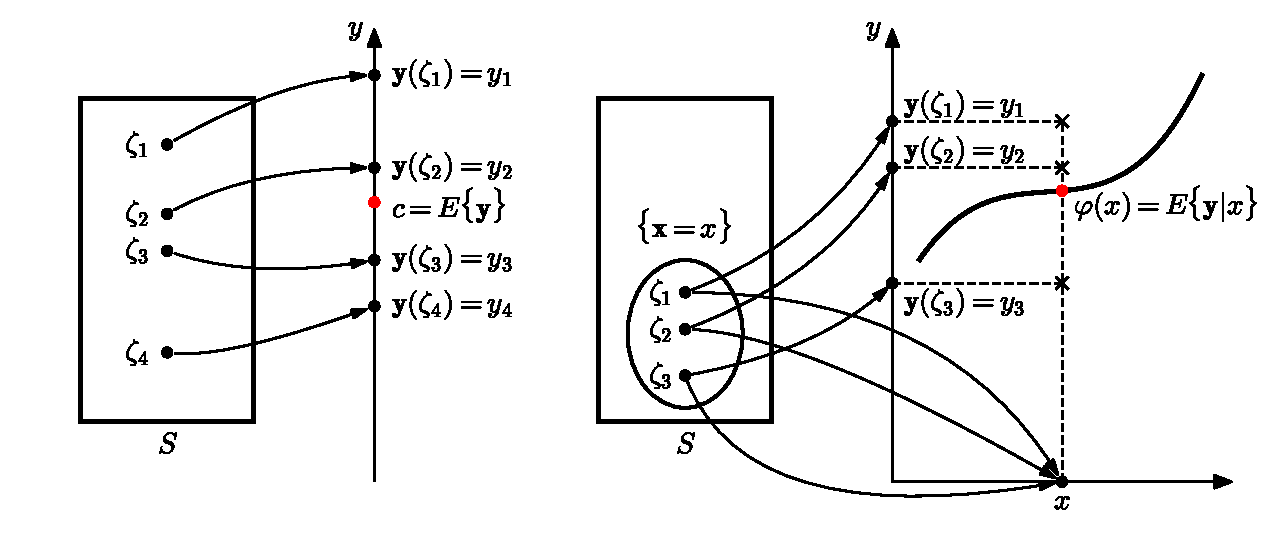
\includegraphics[width=0.97\columnwidth]{figuras/mean_square_estimation_scheme.pdf}
\caption{\label{fig:mean_square_estimation_scheme} Estimación media cuadrática. A la izquierda se esquematiza la estimación media cuadrática de la variable aleatoria \(\y\) mediante una constante \(c\). El valor de \(c\) que minimiza el error cuadrático medio de estimación es la media de \(\y\). A la derecha se ilustra la estimación de \(\y\) a partir de la observación de otra variable aleatoria \(\x\). Si se observa que la variable aleatoria \(\x\) toma el valor \(x\), se sabe que el resultado del experimento pertenece al conjunto \(\{\x=x\}\), que en el ejmplo es \(\{\zeta_1,\,\zeta_2,\,\zeta_3\}\). De esta forma, los resultados posibles de la variable aleatoria \(\y\) son \(\y(\zeta_1)\), \(\y(\zeta_2)\) o \(\y(\zeta_3)\), y la estimación óptima es \(\varphi(x)=E\{\y\,|\,x\}\).}
\end{center}
\end{figure}

Considérese el siguiente ejemplo. Supóngase que el espacio muestral \(S\) es el conjunto de \(n\) niños en una comunidad y la variable aleatoria \(\y\) es la altura de cada niño. Un resultado particular \(\zeta\) es un niño específico. Supóngase además que cada niño seleccionado es pesado, y la variable aleatoria \(\x\) es el peso de cada niño. Al seleccionar un niño \(\zeta_i\) y observar su peso \(\x(\zeta_i)=x\), no queda determinada su altura \(\y(\zeta_i)=y_i\) porque puede haber varios niños con igual peso \(x\) pero distinta altura. Pero al observar el peso \(x\), se sabe que el niño seleccionado es alguno del subconjunto \(\{\x=x\}\) y la incertidumbre se reduce. Por ejemplo, si hubiera solo un niño mas \(\zeta_j\) de peso \(x\), es decir, \(\x(\zeta_j)=x\), al observar el peso \(x\) se sabe que el niño puede ser alguno del subconjunto \(\{\zeta_i,\,\zeta_j\}\) del espacio muestral \(S\), es decir, solo pueden ser dos niños de los \(n\) niños de la comunidad. De esta forma, el valor de la variable aleatoria \(\y\) puede ser solo \(\y(\zeta_i)=y_i\) o \(\y(\zeta_j)=y_j\). El estimador óptimo de \(\y\) es la media condicional \(E\{\y\,|\,x\}\) de \(\y\) dado \(\x=x\), donde \(x\) es el peso observado. En el caso del ejemplo, el estimador óptimo de la altura es el promedio de \(y_i\) e \(y_j\). En el caso de estimar la altura mediante una constante sin observar el peso, el estimador óptimo es el promedio de todas las alturas de los niños, es decir, \(E\{\y\}\). Estas consideraciones se ilustran en la figura \ref{fig:mean_square_estimation_scheme}.

En el contexto de la teoría de probabilidad, el probelma de la estimación cuadratica media (MS, \emph{mean square}) de \(\y\) mediante una constante \(c\) se plantea como sigue: determinar \(c\) de forma tal que el segundo momento \(e\) del error de estimación \(\y-c\) sea mínimo. El segundo momento del error de estimación es
\begin{equation}\label{eq:mse_constant_definition}
 e=E\{(\y-c)^2\}=\int_{-\infty}^{\infty}(y-c)^2f(y)\,dy.
\end{equation}
El valor de \(c\) que minimiza \(e\) se obtiene igualando la derivada de \(e\) respecto a \(c\) a cero. Esta derivada es
\begin{align*}
 \frac{de}{dc}&=\frac{d}{dc}\left[\int_{-\infty}^{\infty}(y-c)^2f(y)\,dy\right]\\
  &=\int_{-\infty}^{\infty}\frac{d}{dc}\left[(y-c)^2\right]f(y)\,dy\\
  &=-\int_{-\infty}^{\infty}2(y-c)f(y)\,dy,
\end{align*}
e igualando a cero, se obtiene que
\[
 \int_{-\infty}^{\infty}(y-c)f(y)\,dy=0\qquad\Leftrightarrow\qquad \int_{-\infty}^{\infty}yf(y)\,dy=c\int_{-\infty}^{\infty}f(y)\,dy=c.
\]
Se concluye que el valor de \(c\) que minimza el error MS de estimación es
\begin{equation}\label{eq:mse_constant}
 c=E\{\y\}=\int_{-\infty}^{\infty}yf(y)\,dy.
\end{equation}
Notar que el mismo razonamiento podría haberse realizado directamente con la esperanza. Efectivamente, la derivada de \(e\) respceto a \(c\) es
\[
 \frac{de}{dc}=\frac{d}{dc}E\{(\y-c)^2\}\overset{(a)}{=}E\left\{\frac{d}{dc}\left[(\y-c)^2\right]\right\}
 =E\{-2(\y-c)\}=2c-2E\{\y\},
\]
donde en \((a)\) se intercambió el orden de la operación derivada y esperanza, que equivale a intercambiar el orden de integración y diferenciación. 

Se considera ahora el caso en que se desea estimar \(\y\) a partir de la observación de otra variable aleatoria \(\x\). El ojetivo es encontrar una función \(c(\x)\) de forma tal que el error MS sea mínimo. Este problema es referido como \emph{estimacion MS no lineal}. El segundo momento \(e\) del error de estimación es
\[
 e=E\{[\y-c(\x)]^2\}=\int_{-\infty}^{\infty}\int_{-\infty}^{\infty}[y-c(x)]^2f(x,\,y)\,dx\,dy.
\]
Para minimziar \(e\), se considera que \(f(x,\,y)=f(y\,|\,x)f(x)\) (ver sección \ref{sec:joint_conditional_distributions}) y por lo tanto
\begin{align*}
  e&=\int_{-\infty}^{\infty}\int_{-\infty}^{\infty}[y-c(x)]^2f(y\,|\,x)f(x)\,dx\,dy\\
   &=\int_{-\infty}^{\infty}f(x)\int_{-\infty}^{\infty}[y-c(x)]^2f(y\,|\,x)\,dy\,dx.
\end{align*}
Como los integrandos son positivos, \(e\) es mínimo si la integral interna es mínima para todo \(x\). Por lo tanto, para minimizar \(e\) alcanza con considerar \(x\) fijo y minimizar la integral interna. Como la integral interna es de la forma de la integral \ref{eq:mse_constant_definition} cambiando \(c\) por \(c(x)\) y \(f(y)\) por \(f(y\,|\,x)\), el mínimo es de la forma de \ref{eq:mse_constant} cambiando \(f(y)\) por \(f(y\,|\,x)\), lo que resulta en
\begin{equation}\label{eq:mse_nonlinear}
 c(x)=E\{\y\,|\,x\}=\int_{-\infty}^{\infty}yf(y\,|\,x)\,dy.
\end{equation}
De esta forma, la función \(c(x)\) óptima es la línea de regresión \(\varphi(x)\), definida en la ecuación \ref{eq:linear_regression}.

Observar que si \(\y=g(\x)\), se cumple que \(E\{\y\,|\,x\}=g(\x)\), ya que
\small
\[
 E\{\y\,|\,x\}=\int_{-\infty}^{\infty}yf(y\,|\,x)\,dy=\int_{-\infty}^{\infty}g(x)f(y\,|\,x)\,dy=g(x)\int_{-\infty}^{\infty}f(y\,|\,x)\,dy=g(x).
\]
\normalsize
Por lo tanto, \(c(x)=g(x)=y\), y el error MS de estimación es nulo. Esto es de esperarse, ya si \(\y=g(\x)\), \(\y\) queda unívocamente determinado a partir de \(\x\). Por otro lado, si \(\x\) e \(\y\) son independientes, \(E\{\y\,|\,x\}=E\{\y\}\) es constante. En este caso, el conocimiento de \(\x\) no aporta nada en la estimación de \(\y\).

\subsection{Estimación cuadrática media lineal}

La solución de la estimación MS no lineal requiere el conocimiento de la función de regresión lineal \(\varphi(x)\). Un problema mas simple, cuya solución solo requiere el conocimiento de los momentos de segundo orden, es la \emph{estimación MS lineal} de \(\y\) en términos de \(\x\), en donde la estimación de \(\y\) se realiza a partir de una función lineal \(A\x+B\) de \(\x\). En este problema hay que determinar las constantes \(A\) y \(B\) de forma de minimizar el error MS
\begin{equation}\label{eq:linear_mse}
 e=E\{[\y-(A\x+B)]^2\}.
\end{equation}
Se demostrará que \(e=e_m\) es mínimo si
\[
 A=\frac{\mu_{11}}{\mu_{20}}=\frac{r\sigma_y}{\sigma_x},\qquad B=\eta_y-A\eta_x,
\]
y el error mínimo es
\[
 e_m=\mu_{02}-\frac{\mu_{11}^2}{\mu_{20}}=\sigma_y^2(1-r^2),
\]
En estas ecuaciones,
\[
 \mu_{ij}=E\{(\x-\eta_x)^i(\y-\eta_y)^j\}
\]
y \(r\) es el coeficiente de correlación, definido en la ecuación \ref{eq:correlation_coefficient_definition}. Además, la segunda igualdad en la ecuación de \(A\) se verifica porque
\[
 A=\frac{\mu_{11}}{\mu_{20}}=\frac{E\{(\x-\eta_x)(\y-\eta_y)\}}{E\{(\x-\eta_x)^2\}}\overset{(a)}{=}\frac{C_{xy}}{\sigma^2_x}\overset{(b)}{=}\frac{r\sigma_x\sigma_y}{\sigma_x^2}=\frac{r\sigma_y}{\sigma_x},
\]
donde en \((a)\) se usó la definición de covarianza, dada en la ecuación \ref{eq:covariance_definition} y  en \((b)\) se usó la ecuación \ref{eq:correlation_coefficient_definition}. De forma similar, la segunda igualdad en la ecuación del error MS mínimo \(e_m\) se verifica porque
\[
 e_m=\mu_{02}-\frac{\mu_{11}^2}{\mu_{20}}=\sigma_y^2-\frac{C_{xy}^2}{\sigma_x^2}
 =\sigma_y^2-\frac{r^2\sigma_x^2\sigma_y^2}{\sigma_x^2}=\sigma_y^2-r^2\sigma_y^2.
\]

Para demostrar estos resultados, se parte observando en la ecuación \ref{eq:linear_mse} del error MS \(e\), que para un valor dado de \(A\), \(e\) es el error MS de la estimación de la variable aleatoria \(\y-A\x\) mediante de la constante \(B\). Por lo tanto, como indica la ecuación \ref{eq:mse_constant}, \(e\) es mínimo si
\[
 B=E\{\y-A\x\}=E\{\y\}-AE\{\x\}=\eta_y-A\eta_x,
\]
con lo que queda determinado \(B\). Para determinar \(A\), se sustituye el valor de \(B\) en la ecuación \ref{eq:linear_mse},
\begin{align*}
 e&=E\{[\y-(A\x+\eta_y-A\eta_x)]^2\}\\
  &=E\{[(\y-\eta_y)-A(\x-\eta_x)]^2\}\\
  &=E\{(\y-\eta_y)^2\}+A^2E\{(\x-\eta_x)^2\}-2AE\{(\x-\eta_x)(\y-\eta_y)\}\\
  &=\sigma_y^2+A^2\sigma_x^2-2AC_{xy},
\end{align*}
resultando en
\begin{equation}\label{eq:linear_mse_deduction_tmp1}
 e=\sigma_y^2+A^2\sigma_x^2-2Ar\sigma_x\sigma_y.
\end{equation}
Igualando la derivada de \(e\) respecto a \(A\) a cero,
\[
 \frac{de}{dA}=2A\sigma_x^2-2r\sigma_x\sigma_y=0,
\]
y despejando \(A\), se obtiene que
\[
 A=\frac{r\sigma_y}{\sigma_x}.
\]
Finalmente, el error mínimo se obtiene sustituyendo el valor de \(A\) óptimo en la ecuación \ref{eq:linear_mse_deduction_tmp1},
\[
 e_m=\sigma_y^2+\left(\frac{r\sigma_y}{\sigma_x}\right)^2\sigma_x^2-2\left(\frac{r\sigma_y}{\sigma_x}\right)r\sigma_x\sigma_y=\sigma_y^2+r^2\sigma_y^2-2r^2\sigma_y^2
 =\sigma_y^2(1-r^2).
\]

\paragraph{Terminología} El estimador \(A\x+B\) se dice estimador lineal \emph{no homogéneo} de \(\y\) en términos de \(\x\). Si \(\y\) es estimada por una línea recta \(A\x\) que pasa por el origen, el estimador se dice \emph{homogéneo}. 

La variable aleatoria \(\x\) es el dato de la estimación, la variable aleatoria \(\varepsilon=\y-(A\x+B)\) es el \emph{error} de estimación y el valor \(e=E\{\varepsilon^2\}\) es el \emph{error cuadrático medio} de estimación.

\paragraph{Variable aleatorias conjuntamente normales} En general, el estimador no lineal \(\varphi(x)=E\{\y\,|\,x\}\) de \(\y\) en términos de \(\x\) no es una recta, y el error MS de estimación \(E\{[\y-\varphi(\x)]^2\}\) resultante es menor que el error MS \(e_m\) del estimador lineal \(A\x+B\). Sin embargo, si las variables aleatorias \(\x\) e \(\y\) son conjuntamente normales, se cumple que
\[
 \varphi(x)=E\{\y\,|\,x\}=\frac{r\sigma_yx}{\sigma_x}+\eta_y-\frac{r\sigma_y\eta_x}{\sigma_x},
\]
como se puede deducir de la ecuación \ref{eq:joint_normal_conditional_pdf} de \(f(x\,|\,y)\) cambiando \(x\) por \(y\). Observando de \(\varphi(x)\) es una recta, se concluye que si las variables aleatorias son conjuntamente normales, el estimador no lineal y el estimador lineal son idénticos.

\subsection{Principio de ortogonalidad}

El \emph{principio de ortogonalidad} indica que el estimador lineal óptimo \(A\x+B\) de la variable \(\y\) es tal que el error de estimación \(\y-(A\x+B)\) es ortogonal al dato \(\x\). Matemáticamente, esto se expresa como
\begin{equation}\label{eq:linear_mse_orthogonality_principle}
 E\{[\y-(A\x+B)]\x\}=0.
\end{equation}
Para demostrarlo, se observa que los valores de \(A\) y \(B\) que conducen al error MS mínimo se obtienen resolviendo el sistema de ecuaciones \(\partial e/\partial A=0\) y \(\partial e/\partial B=0\), con \(e\) dado por la ecuación \ref{eq:linear_mse}. Derivando el error MS respecto a \(A\), se obtiene que
\begin{align*}
 \frac{\partial e}{\partial A}&=\frac{\partial}{\partial A}\left(E\{[\y-(A\x+B)]^2\}\right)\\
  &\overset{(a)}{=}E\left\{\frac{\partial}{\partial A}[\y-(A\x+B)]^2\right\}\\
  &=E\left\{2[\y-(A\x+B)](-A\x)\right\}\\
  &=-2AE\left\{[\y-(A\x+B)]\x\right\},
\end{align*}
donde en \((a)\) se intercambió el orden de las operaciones de diferenciación y esperanza. Igualando el resultado a 0, se obtiene la ecuación \ref{eq:linear_mse_orthogonality_principle}.

\paragraph{Estimación lineal MS homogénea} Se pretende encontrar la constante \(a\) de forma tal que si \(\y\) es estimada a partir de \(a\x\), el error MS
\begin{equation}\label{eq:homogeneous_linear_ms}
 e=E\{(\y-a\x)^2\}.
\end{equation}
sea mínimo. Derivando respecto a \(a\) e igualando el resultado a cero, se deduce que \(a\) debe cumplir que
\begin{equation}\label{eq:homogeneous_linear_mse_orthogonality}
 E\{(\y-a\x)\x\}=0.
\end{equation}
Despejando \(a\), se obtiene que
\[
 E\{\x\y\}=aE\{\x^2\}\qquad\Rightarrow\qquad a=\frac{E\{\x\y\}}{E\{\x^2\}}.
\]
El estimador MS lineal de \(\y\) en términos de \(\x\) se denotará como \(\hat{E}\{\y\,|\,\x\}\). Por lo tanto, en la estimación lineal homogénea se tiene que
\[
 \hat{E}\{\y\,|\,\x\}=a\x,\qquad a=\frac{E\{\x\y\}}{E\{\x^2\}}.
\]
Se deducirá a continuación la expresión del error MS mínimo. Desarrollando la ecuación \ref{eq:homogeneous_linear_ms}, el error MS puede expresarse por un lado como
\[
 e=E\{(\y-a\x)(\y-a\x)\}=E\{(\y-a\x)\y\}-aE\{(\y-a\x)\x\}.
\]
Por otro lado, \(e\) también se puede escribir como
\[
 e=E\{\y^2\}-E\{(a\x)^2\}-2aE\{(\y-a\x)\x\},
\]
ya que, operando sobre el lado derecho de la igualdad, se observa que
\begin{align*}
  E\{\y^2\}-E\{(a\x)^2\}-2aE\{(\y-a\x)\x\}&=E\{\y^2\}-E\{(a\x)^2\}-E\{2\y(a\x)\}+2E\{(a\x)^2\}\\
   &=E\{\y^2\}+E\{(a\x)^2\}-E\{2\y(a\x)\}\\
   &=E\{\y^2+(a\x)^2-2\y(a\x)\}\\
   &=E\{(\y-a\x)^2\}\\
   &=e.
\end{align*}
Igualando ambas ecuaciones, se tiene que el error MS cumple que
\[
 e=E\{(\y-a\x)\y\}-aE\{(\y-a\x)\x\}=E\{\y^2\}-E\{(a\x)^2\}-2aE\{(\y-a\x)\x\}.
\]
Como el error MS mínimo se obtiene con el valor de \(a\) que verifica la ecuación \ref{eq:homogeneous_linear_mse_orthogonality}, se concluye que el error MS mínimo cumple que
\begin{equation}\label{eq:homogeneous_linear_mse_pythagoras}
  e=E\{(\y-a\x)\y\}=E\{\y^2\}-E\{(a\x)^2\}.
\end{equation}

Se realizarán algunas consideraciones sobre el principio de ortogonalidad. La ecuación \ref{eq:homogeneous_linear_mse_orthogonality} se trata del principio de ortogonalidad, ya que indica que el error de estimación \(\y-a\x\) es ortogonal al dato \(\x\). Para una interpretación geométrica del principio de ortogonalidad, observar la figura \ref{fig:mse_linear_homogeneous} de la representación vectorial de las variables aleatorias involucradas. Por ser \(a\) una constante, la estimación \(a\x\) de \(\y\) es colineal con \(\x\). La diferencia \(\y-a\x\) es el vector que va desde \(a\x\) hasta \(\y\). El largo de este vector es \(\sqrt{E\{(\y-a\x)^2\}}=\sqrt{e}\). Claramente, esta distancia es mínima si se elige \(a\) de forma tal que \(\y-a\x\) es perpendicular con \(\x\), como indica la ecuación \ref{eq:homogeneous_linear_mse_orthogonality}. Observar además que el lado derecho de la ecuación \ref{eq:homogeneous_linear_mse_pythagoras} es teorema de Pitágoras. Efectivamente, en el triángulo rectángulo en la figura, el cuadrado del largo de la hipotenusa es \(E\{\y^2\}\) y el cuadrado del largo de los catetos es \(E\{(a\x)^2\}\) y \(e\). La primera igualdad de la ecuación \ref{eq:homogeneous_linear_mse_pythagoras} indica que el cuadrado del largo de \(\y-a\x\) es el producto interno de \(\y\) con el error \(\y-a\x\).
\begin{figure}[!htb]
  \begin{minipage}[c]{0.52\textwidth}
    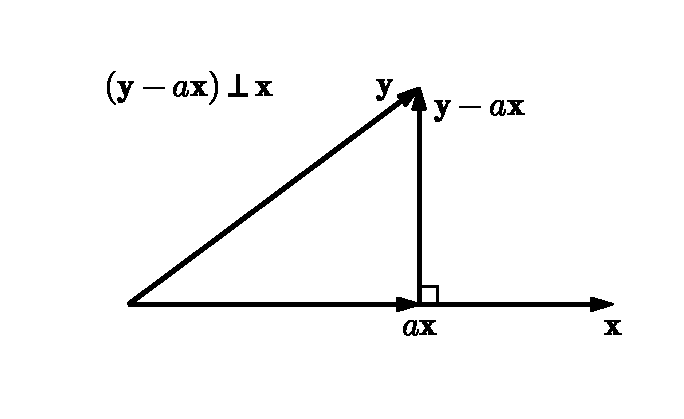
\includegraphics[width=\textwidth]{figuras/mse_linear_homogeneous.pdf}
  \end{minipage}\hfill
  \begin{minipage}[c]{0.45\textwidth}
    \caption{
       Representación vectorial de las variables aleatorias en la estimación MS lineal homogénea de \(\y\) en términos de \(\x\). El valor de \(a\) que minimiza el largo del vector \(\y-a\x\), que representa el error MS de estimación, es el que hace que el vector \(\y-a\x\) sea perpendicular con \(\x\).
    }\label{fig:mse_linear_homogeneous}
  \end{minipage}
\end{figure}

\paragraph{Funciones de riesgo y de pérdida} Se realizarán algunas consideraciones sobre otros criterios de optimización en la estimación de una variable aleatoria \(\y\) mediante una constante \(c\). Se elige una función \(L(x)\) y se determina \(c\) de forma de minimizar la media de la variable aleatoria \(L(\y-c)\),
\[
 R=E\{L(\y-c)\}=\int_{-\infty}^{\infty}L(y-c)f(y)\,dy.
\]
La función \(L(x)\) se llama \emph{función de pérdida} y la constante \(R\) se llama \emph{riesgo promedio}. La elección de \(L(x)\) depende de la aplicación. En el caso en que \(L(x)=x^2\), \(R=E\{(\y-c)^2\}\) es el error MS, el cual se minimiza si \(c=E\{\y\}\).

Si \(L(x)=|x|\), \(R=E\{|\y-c|\}\). Se mostrará que en este caso, el valor de \(c\) que minimiza \(R\) es la \emph{mediana} \(y_{0.5}\) de \(\y\). Para ver esto, se comienza planteando el riesgo promedio,
\[
 R=\int_{-\infty}^{\infty}|y-c|f(y)\,dy\overset{(a)}{=}\int_{-\infty}^{c}(c-y)f(y)\,dy+\int_{c}^{\infty}(y-c)f(y)\,dy,
\]
donde en \((a)\) se tuvo en cuenta que
\[
 |y-c|=
 \left\{\begin{array}{ll}
  y-c, & y\geq c \\
  c-y, & c > y.
 \end{array} \right.
\]
Aplicando la regla de integración de Leibnitz (ecuaciones \ref{eq:leibnitz_integration_rule1} y \ref{eq:leibnitz_integration_rule2}) para diferenciar \(R\) respecto a \(c\), se tiene que
\[
 \frac{dR}{dc}=\int_{-\infty}^{c}f(y)\,dy-\int_{c}^{\infty}f(y)\,dy=F(c)-[1-F(c)]=2F(c)-1,
\]
y al igualar la derivada a cero, se llega a que \(R\) es mínimo si \(F(c)=1/2\), es decir, si \(c=y_{0.5}\).

\subsection{Estimación cuadrática media lineal: caso general}

El estimador lineal MS de la variable aleatoria \(\s\) en términos de las \(n\) variables aleatorias \(\x_i\) es
\[
 \hat{\s}=a_1\x_1+\cdots+a_n\x_n,
\]
donde \(a_1,\dots, a_n\) son constantes tales que el valor MS del error de estimación
\begin{equation}\label{eq:linear_general_case_mse}
 P=E\{(\s-\hat{\s})^2\}=E\{[s-(a_1\x_1+\cdots+a_n\x_n)]^2\}
\end{equation}
sea mínimo.

Se demostrará el \emph{principio de ortogonalidad} para esto caso, que indica que \(P\) es mínimo si el error \(\s-\hat{\s}\) es ortogonal a los datos \(\x_i\), es decir,
\begin{equation}\label{eq:linear_general_case_mse_orthogonality}
  E\{[s-(a_1\x_1+\cdots+a_n\x_n)]\x_i\}=0,\qquad i=1,\dots,\,n.
\end{equation}
Para demostrarlo, basta igualar a cero las derivadas de \(P\) respecto a las constantes \(a_i\),
\[
 \frac{dP}{da_i}=E\{-2[\s-(a_1\x_1+\cdots+a_n\x_n)]\x_i\}=0,
\]
resultando en la ecuación \ref{eq:linear_general_case_mse_orthogonality}. Este resultado se denomina \emph{teorema de la proyección}. Para obtener las constantes que minimizan el error MS de estimación, se establece \(i=1,\dots,\,n\) en la ecuación \ref{eq:linear_general_case_mse_orthogonality}, resultando en el sistema de ecuaciones
\begin{equation}\label{eq:linear_general_case_mse_coeficients_system}
 \arraycolsep=1.4pt\def\arraystretch{1.4}
 \left\{\begin{array}{ccccccccc}
   R_{11}a_1&+&R_{21}a_2&+&\cdots&+&R_{n1}a_n&=&R_{01}\\
   R_{12}a_1&+&R_{22}a_2&+&\cdots&+&R_{n2}a_n&=&R_{02}\\
   \vdots   & &\vdots   & &      & &\vdots   & &\vdots\\
   R_{1n}a_1&+&R_{2n}a_2&+&\cdots&+&R_{nn}a_n&=&R_{0n}\\
 \end{array}\right.,
\end{equation}
donde \(R_{ij}=E\{\x_i\x_j\}\) y \(R_{0j}=E\{\s\x_j\}\). Definiendo los vectores fila
\[
 \X=[\x_1,\dots,\,\x_n],\qquad A=[a_1,\dots,\,a_n],\qquad R_0=[R_{01},\dots,\,R_{0n}]
\]
y la matriz de correlación de los datos \(R=\X^t\X\), el sistema de ecuaciones se puede expresar como
\[
 AR=R_0,
\]
y su solución es
\begin{equation}\label{eq:linear_general_case_mse_coeficients}
 A=R_0R^{-1}.
\end{equation}

Sustituyendo la ecuación \ref{eq:linear_general_case_mse_coeficients} en la ecuación \ref{eq:linear_general_case_mse} se obtiene el error MS mínimo de estimación (LMS, \emph{least mean square}). Para hacerlo, se parte expresando la ecuación \ref{eq:linear_general_case_mse} de forma vectorial y se opera como sigue,
\begin{align*}
 P&=E\left\{\left(\s-A\X^t\right)^2\right\}\\
  &=E\{\s^2\}-2AE\{\s\X^t\}+E\left\{\left(A\X^t\right)^2\right\}\\
  &\overset{(a)}{=}E\{\s^2\}-2AR_0^t+AE\left\{\X^t\X\right\}A^t\\
  &=E\{\s^2\}-2AR_0^t+ARA^t,
\end{align*}
donde en \((a)\) se empleó que \(E\{\s\X^t\}=R_0^t\) en el segundo sumando, como fue definido previamente, y en el tercer sumando se observó que como \(A\X^t\) es un escalar, se cumple que \((A\X^t)^2=(A\X^t)(A\X^t)^t=A\X^t\X A^t\). Para obtener el error LMS, se sustituye \(A^t\) en el tercer sumando de \(P\) por los coeficientes óptimos, dados por la ecuación \ref{eq:linear_general_case_mse_coeficients}. De esta forma, ese tercer sumando queda
\[
 ARA^t=AR(R_0R^{-1})^t=AR\left(R^{-1}\right)^tR_0^t=AR\left(R^t\right)^{-1}R_0^t
 \overset{(a)}{=}ARR^{-1}R_0^t=AR_0^t,
\]
donde en \((a)\) se consideró que la matriz \(R\) es simétrica y por lo tanto \(R^t=R\).
Se concluye que el error LMS es
\begin{equation}\label{eq:linear_general_case_mse_error}
 P=E\{\s^2\}-AR_0^t.
\end{equation}

Otra forma de obtener el error LMS, es observando que como \(\s-\hat{\s}\perp\x_i\) para todo \(i\), se cumple que \(\s-\hat{\s}\perp\hat{\s}\). Efectivamente,
\begin{align*}
 E\{(\s-\hat{\s})\hat{\s}\}&=E\{(\s-\hat{\s})(a_1\x_1+\cdots+a_n\x_n)\}\\
  &=a_1E\{(\s-\hat{\s})\x_1\}+\cdots+a_nE\{(\s-\hat{\s})\x_n\}\\
  &=0.
\end{align*}
Teniendo esto en cuenta, la ecuación \ref{eq:linear_general_case_mse} del error MS queda
\[
 P=E\{(\s-\hat{\s})(\s-\hat{\s})\}=E\{(\s-\hat{\s})\s\}-E\{(\s-\hat{\s})\hat{\s}\}=E\{(\s-\hat{\s})\s\},
\]
y considerando que
\[
 E\{\hat{\s}\s\}=E\{A\X^t\s\}=AE\{\X^t\s\}=AR_0^t,
\]
se obtiene que
\[
 P=E\{(\s-\hat{\s})\s\} = E\{\s^2\}-AR_0^t.
\]

Como interpretación geométrica de este resultado, se observa que en la representación de las variables aleatorias en un espacio vectorial, la suma \(a_1\x_1+\cdots+a_n\x_n\) es un vector del subespacio \(S_n\) de los datos \(\x_i\). El error \(\varepsilon=\s-\hat{\s}\) es el vector que va desde \(\hat{\s}\) a \(\s\), como se muestra en la figura \ref{fig:mse_linear_general_case}. El teorema de la proyección indica que el largo de \(\varepsilon\) es mínimo si \(\varepsilon\) es ortogonal a los datos \(\x_i\), es decir, si es perpendicular al subespacio \(S_n\). Por lo tanto, el estimador \(\hat{\s}\) es la proyección de \(\s\) en el subespacio \(S_n\).
\begin{figure}[!htb]
  \begin{minipage}[c]{0.52\textwidth}
    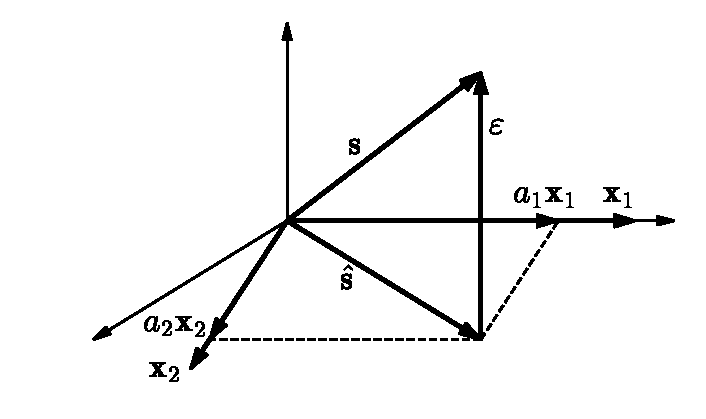
\includegraphics[width=\textwidth]{figuras/mse_linear_general_case.pdf}
  \end{minipage}\hfill
  \begin{minipage}[c]{0.45\textwidth}
    \caption{
       Representación vectorial de las variables aleatorias en el caso general de la estimación MS lineal. En el ejemplo de la figura, se estima \(\s\) en términos de \(\x_1\) y \(\x_2\). El estimador LMS es la proyección de \(\s\) en el plano determinado por \(\x_1\) y \(\x_2\). El error de estimación \(\varepsilon=\s-\hat{\s}\) es perpendicular a dicho plano.
    }\label{fig:mse_linear_general_case}
  \end{minipage}
\end{figure}

Se consideran a continuación dos casos particulares. Si \(\s\) es un vector del subespacio \(S_n\), \(\hat{\s}=\s\), resultando en \(P=0\). En este caso, las \(n+1\) variables aleatorias \(\s,\,\x_1,\dots,\x_n\) son linealmente dependientes y el determinante \(\Delta_{n+1}\) de la matriz de correlación es cero. Por otro lado, si \(\s\) es perpendicular a \(S_n\), \(\hat{\s}=0\), resultando en \(P=E\{|\s|^2\}\). En esta situación, \(\s\) es ortogonal a los datos \(\x_i\), y \(R_{0j}=0\) si \(j\neq0\).

\subsection{Estimación cuadrática media no lineal: caso general}

El problema de estimación MS no lineal consiste en determinar la función \(g(\x_1,\dots,\,\x_n)=g(\X)\) de los datos \(\x_i\) de forma de minimizar el error MS
\[
 P=E\{[\s-g(\X)]^2\}.
\]
Se demostrará que \(P\) es mínimo si
\begin{equation}\label{eq:nonlinear_general_case_mse}
 g(X)=E\{\s\,|\,X\}=\int_{-\infty}^{\infty}sf_s(s\,|\,X)\,ds.
\end{equation}
\(E\{\s\,|\,X\}\), la media condicional de la variable \(\s\) asumiendo que \(\X=X\), es una función de \(X\) y se denomina superficie de regresión. 

Para demostrar que el estimador MS está dado por la ecuación \ref{eq:nonlinear_general_case_mse} se parte de la siguiente identidad
\[
 P=E\{[\s-g(\X)]^2\}=E\{E\{[\s-g(\X)]^2\,|\,\X\}\},
\]
la cual se justifica con lo indicado en las secciones \ref{sec:conditional_expected_values_as_rv} y \ref{sec:conditional_expected_values_as_rv_sequence}. El último termino en esta igualdad expresado explícitamente como una integral es
\[
 P=\int_{-\infty}^{\infty}\left\{\int_{-\infty}^{\infty}[s-g(X)]^2f_s(s\,|\,X)\,ds\right\}f(X)\,dX,
\]
donde la integral interna corresponde a la esperanza condicional interna, y la integral externa es una integral múltiple de multiplicidad \(n\), es decir, la cantidad de datos \(\x_i\). Como todas las funciones del integrando son positivas, \(P\) es mínimo si la integral interna es mínima para todo \(X\). Por lo tanto, para minimizar \(P\), se considera \(X\) fijo y se minimiza el error MS condicional
\[
 E\{[\s-g(\X)]^2\,|\,X\}=\int_{-\infty}^{\infty}[s-g(\X)]^2f_s(s\,|\,X)\,ds.
\]
Como esta integral es análoga a la integral que se minimizó en la deducción de la ecuación \ref{eq:mse_nonlinear}, se concluye que la integral es mínima si \(g(X)\) está dada por la ecuación \ref{eq:nonlinear_general_case_mse}.

\paragraph{Principio de ortogonalidad general}

Del teorema de la proyección dado por la ecuación \ref{eq:linear_general_case_mse_orthogonality} se deduce que para el estimador MS lineal \(\hat{\s}\) se cumple que
\[
 E\{[\s-\hat{\s}](c_1\x_1+\cdots+c_n\x_n)\}=0
\]
para cualquier conjunto de valores \(c_1,\dots,\,c_n\). Esto indica que si \(\hat{\s}\) es el estimador lineal de \(\s\), el error de estimación \(\s-\hat{\s}\) es ortogonal a cualquier función lineal \(\y=c_1\x_1+\cdots+c_n\x_n\) de los datos \(\x_i\).

Se demostrará que si \(g(\X)\) es el estimador MS no lineal de \(\s\), el error de estimación \(\s-g(\X)\) es ortogonal a cualquier función \(w(\X)\), lineal o no lineal, de los datos \(\x_i\), es decir,
\begin{equation}\label{eq:general_orthongonal_principle}
  E\{[\s-g(\X)]w(\X)\}=0.
\end{equation}
Se demostrará previamente la identidad
\begin{equation}\label{eq:general_orthongonal_principle_tmp}
  E\{[\s-g(\X)]w(\X)\}=E\{w(\X)E\{[\s-g(\X)]\,|\,\X\}\},
\end{equation}
que es una generalización de las esperanzas condicionales deducidas en la sección \ref{sec:conditional_expected_values_as_rv}. En esta identidad, la esperanza condicional interna del lado derecho es la variable aleatoria
\[
 E\{[\s-g(\X)]\,|\,\X\}=\int_{-\infty}^{\infty}[s-g(\X)]f_s(s\,|\,\X)\,ds.
\]
Al multiplicar por \(w(\X)\) y tomar esperanza, se tiene que
\begin{align*}
 E\{w(\X)E\{[\s-g(\X)]\,|\,\X\}\}&=\int_{-\infty}^{\infty}w(X)\left\{\int_{-\infty}^{\infty}[s-g(X)]f_s(s\,|\,X)\,ds\right\}f(X)\,dX\\
 &=\int_{-\infty}^{\infty}\int_{-\infty}^{\infty}w(X)[s-g(X)]f_s(s\,|\,X)f(X)\,ds\,dX
\end{align*}
y considerando que \(f_s(s\,|\,X)f(X)=f(s,\,X)\) (ecuación \ref{eq:sequence_rv_conditional_joint_densities}), se obtiene que
\begin{align*}
 E\{w(\X)E\{[\s-g(\X)]\,|\,\X\}\}&=\int_{-\infty}^{\infty}\int_{-\infty}^{\infty}w(X)[s-g(X)]f(s,\,X)\,ds\,dX\\
 &=E\{[\s-g(\X)]w(\X)\},
\end{align*}
que es lo que se quería demostrar. Para demostrar la ecuación \ref{eq:general_orthongonal_principle} se opera sobre la esperanza interna en el lado derecha de la identidad \ref{eq:general_orthongonal_principle_tmp},
\[
 E\{[\s-g(\X)]\,|\,X\}\overset{(a)}{=}E\{\s\,|\,X\}-E\{g(\X)\,|\,X\}
 \overset{(b)}{=}E\{\s\,|\,X\}-g(X)\overset{(c)}{=}0,
\]
donde en \((a)\) se aplicó la propiedad de linealidad de la esperanza, en \((b)\) se consideró que \(E\{g(\X)\,|\,X\}=E\{g(X)\}=g(X)\) y en \((c)\) se consideró que \(g(X)\) es el estimador MS no lineal y por lo tanto se cumple la ecuación \ref{eq:nonlinear_general_case_mse}. Se concluye que el término de la derecha de la identidad \ref{eq:general_orthongonal_principle_tmp} es nulo, resultando en la ecuación \ref{eq:general_orthongonal_principle}.

\paragraph{Normalidad} Se demostrará que si las variables aleatorias \(\s,\,\x_1,\dots,\,\x_n\) son conjuntamente normales con media nula, el estimador lineal y el estimador no lineal de \(\s\) son iguales,
\begin{equation}\label{eq:mse_normal_rv}
  \hat{\s}=a_1\x_1+\dots+\x_n=g(\X)=E\{\s\,|\,\X\}.
\end{equation}
Para demostrarlo, hay que demostrar que \(\hat{\s}=E\{\s\,|\,\X\}\). Como \(\s-\hat{\s}\) es una combinación lineal de variables aleatorias conjuntamente normales, las variables aleatorias \(\s-\hat{\s}\) y \(\x_i\) son conjuntamente normales y \(\s-\hat{\s}\) tiene media nula. Además, como  \(\s-\hat{\s}\) es el error de estimación mínimo, es ortogonal a los datos \(\x_i\) y se cumple que \(E\{(\s-\hat{\s})\x_i\}=0\). Esto implica que su covarianza es nula y por lo tanto son no correlacionadas. Se concluye que  \(\s-\hat{\s}\) y \(\x_i\) son variables aleatorias no correlacionadas, ya que su covarianza es nula, y conjuntamente normales, y por lo tanto, independientes, como se explicó en la sección \ref{sec:uncorrelation_and_onthogonality}. Entonces, por un lado se tiene que
\[
 E\{\s-\hat{\s}\,|\,X\}=E\{\s\,|\,X\}-E\{\hat{\s}\,|\,X\}=E\{\s\,|\,X\}-\hat{\s},
\]
donde en la última igualdad se consideró que \(\hat{\s}\) es una función de \(\X\), por lo que \(E\{\hat{\s}(\X)\,|\,X\}=E\{\hat{\s}(X)\}=\hat{\s}\). Además, por otro lado se tiene que
\[
 E\{\s-\hat{\s}\,|\,X\}=E\{\s-\hat{\s}\}=E\{\s\}-E\{\hat{\s}\}=0,
\]
donde en la primera igualdad se consideró que \(\s-\hat{\s}\) y \(\X\) son variables aleatorias independientes y en la última igualdad, que \(E\{\s\}=E\{\hat{\s}\}=0\). Combinando los dos resultados, se obtiene que \(\hat{\s}=E\{\s\,|\,X\}\), que es lo que se quería demostrar.

\paragraph{Densidades condicionales de variables aleatorias normales} Se emplearán los resultados anteriores para determinar de forma simple las densidades de probabilidad condicional de variables aleatorias normales. La densidad de probabilidad condicional de \(\s\) dado \(\X\) es 
\[
 f(s\,|\,X)=\frac{f(s,\,X)}{f(X)},
\]
y como consiste en el cociente de dos exponenciales de exponentes cuadráticos, también es una densidad normal. Para establecerla, basta con determinar la media \(\mu_{s|X}\) y la varianza \(\sigma^2_{s|X}\). La media es
\[
 \mu_{s|X}=E\{\s\,|\,X\}=\hat{s},
\]
como indica la ecuación \ref{eq:mse_normal_rv}. La varianza es
\[
 \sigma^2_{s|X}=E\{(\s-\hat{\s})^2\,|\,X\}\overset{(a)}{=}E\{(\s-\hat{\s})^2\}\overset{(b)}{=}P,
\]
donde en \((a)\) se consideró que \(\s-\hat{\s}\) y \(\X\) son variables aleatorias independientes y en \((b)\) se empleó la ecuación \ref{eq:linear_general_case_mse}, donde \(P\) es el error MS mínimo. Por lo tanto, se concluye que
\[
 f(s\,|\,x_1,\dots,\,x_n)=\frac{1}{\sqrt{2\pi P}}e^{-[s-(a_1x_1+\cdots+a_nx_n)]^2/2P},
\]
donde los coeficientes \(a_i\) se obtienen mediante la ecuación \ref{eq:linear_general_case_mse_coeficients} y el error MS mínimo mediante la ecuación \ref{eq:linear_general_case_mse_error}.

\paragraph{Ejemplo (7-12)} Se consideran las variables aleatorias \(\x_1\), \(\x_2\) y \(\x_3\) conjuntamente normales y de media nula. Se quiere determinar la densidad de probabilidad \(f(x_3\,|\,x_1,\,x_2)\).

Por la argumentación indicada previamente, \(f(x_3\,|\,x_1,\,x_2)\) es una densidad de probabilidad normal, y para determinarla, alcanza con calcular la media \(\mu_{x_3|x_1,x_2}\) y la varianza \(\sigma^2_{x_3|x_1,x_2}\). La media es el estimador MS lineal,
\[
 \mu_{x_3|x_1,x_2}=E\{\x_3|\x_1,\x_2\}=\hat{\s}=a_1\x_1+a_2\x_2,
\]
por lo que para determinar los coeficientes \(a_1\) y \(a_2\) hay que resolver el sistema \ref{eq:linear_general_case_mse_coeficients_system}, que en el caso de dos coeficientes queda
\[
 \arraycolsep=1.4pt\def\arraystretch{1.4}
 \left\{\begin{array}{ccccc}
   R_{11}a_1&+&R_{12}a_2&=&R_{13}\\
   R_{12}a_1&+&R_{22}a_2&=&R_{23}
 \end{array}\right.,
\]
donde \(R_{ij}=E\{\x_{i}\x_{j}\}=R_{ji}\). Al resolver el sistema, se obtiene que
\[
 a_1=\frac{R_{12}R_{23}-R_{22}R_{13}}{R_{12}^2-R_{11}R_{22}},\qquad
 a_2=\frac{R_{12}R_{13}-R_{11}R_{23}}{R_{12}^2-R_{11}R_{22}}.
\]
La varianza se obtiene mediante la ecuación \ref{eq:linear_general_case_mse_error}, y en este caso queda
\[
 \sigma^2_{x_3|x_1,x_2}=P=R_{33}-({a_1R_{13}+a_2R_{23}}).
\]
De esta forma la densidad buscada es
\[
 f(x_3\,|\,x_1,\,x_2)=\frac{1}{\sqrt{2\pi P}}e^{-[x_3-(a_1x_1+a_2x_2)]^2/2P}.
\]

\section{Convergencia estocástica y teoremas de límite}

Un problema importante en la teoría de la probabilidad es el estudio de las propiedades asintóticas de secuencias de variables aleatorias. En esta sección se introducen los conceptos asociados, haciendo énfasis en las definiciones de los distintos modos de convergencia y la relación entre ellos.

\paragraph{Ejemplo} Considérese el caso en que se quiere medir el largo \(a\) de un objeto. Debido a los errores de medida, la lectura del instrumento es
\[
 \x=a+\mathbf{v},
\]
donde \(\mathbf{v}\) es un término de error. Si no hay errores sistemáticos de medición, \(\mathbf{v}\) es una variable aleatoria de media nula. Si la desviación estándar \(\sigma\) de \(\mathbf{v}\) es pequeña en comparación a \(a\), el valor observado \(\x(\zeta)\) de \(\x\) en una única medida es un buen estimador del parámetro desconocido \(a\).
En el contexto de la teoría de probabilidad, esta conclusión se puede expresar cuantitativamente como sigue: la media de la variable aleatoria \(\x\) es \(a\), ya que
\[
 E\{\x\}=E\{a+\mathbf{v}\}\overset{(a)}{=}E\{a\}+E\{\mathbf{v}\}\overset{(b)}{=}a,
\]
donde en \((a)\) se empleó la propiedad de linealidad de la esperanza y en \((b)\) que como \(a\) es una constante, \(E\{a\}=a\), y también que el error de medición es de media nula, \(E\{\mathbf{v}\}=0\). Además, la varianza \(\sigma^2_x\) de \(\x\) es \(\sigma^2\), ya que
\[
 \sigma^2_x=E\{(\x-E\{\x\})^2\}=E\{(a+\mathbf{v}-a)^2\}=E\{\mathbf{v}^2\}=\sigma^2,
\]
donde en la última igualdad se empleó que \(\mathbf{v}\) es de media nula. Por lo tanto, a partir del complemento de la desigualdad de Chebyshev (ecuación \ref{eq:chebyshev_inequality}), se tiene que
\[
 P\{|\x-a|<\epsilon\}\geq 1-\frac{\sigma^2}{\epsilon^2}.
\]
De esta forma, si \(\sigma\ll\epsilon\), la probabilidad de que \(|\x-a|\) sea menor que \(\epsilon\) es cercana a 1. Esto significa que ``casi certeramente'' el valor observado \(\x(\zeta)\) estará entre \(a-\epsilon\) y \(a+\epsilon\) o equivalentemente, el parámetro desconocido \(a\) estará entre \(\x(\zeta)-\epsilon\) y \(\x(\zeta)+\epsilon\). En resumen, una única medida \(\x(\zeta)\) es un estimador de \(a\) ``casi certeramente'' satisfactorio si \(\sigma\ll a\). Si \(\sigma\) no es pequeño en comparación a \(a\), una única medida no es suficiente para obtener una buen estimador de \(a\). En ese caso, para incrementar la exactitud de la medición, pueden realizarse varias lecturas y promediar los resultados. Supóngase que se realizan \(n\) lecturas independientes. La lectura  \(i\)-ésima es
\[
 \x_i=a+\mathbf{v}_i,
\]
donde los componentes de error \(\mathbf{v}_i\) son variables aleatorias independientes de media nula y varianza \(\sigma^2\). La media muestral
\[
 \bar{\x}=\frac{\x_1+\dots+\x_n}{n}
\]
de las lecturas tiene media \(a\) y varianza \(\sigma^2/n\), como se explicó en la sección \ref{sec:sample_mean_and_variance}. Por lo tanto, si \(n\) es suficientemente grande de forma que \(\sigma^2\ll na\), el valor \(\bar{\x}(\zeta)\) de la media muestral \(\bar{\x}\) en un único experimento de \(n\) medidas es un buen estimador de \(a\). Supóngase que la cantidad de lecturas \(n\) es tal que \(\sigma^2/na^2=10^{-4}\) y se quiere calcular la probabilidad de que \(\bar{\x}\) esté entre \(0.9a\) y \(1.1a\). Para hacerlo, se recurre a la desigualdad de Chebyshev (ecuación \ref{eq:chebyshev_inequality}) y se observa que
\[
 |\bar{\x}-a|<\epsilon\qquad\Leftrightarrow\qquad -\epsilon<\bar{\x}-a<\epsilon
 \qquad\Leftrightarrow\qquad a-\epsilon<\bar{\x}<a+\epsilon,
\]
y como se busca que \(0.9a<\mathbf{\x}<1.1a\), \(\epsilon=0.1a\) en la desigualdad. De esta forma,
\[
  P\{0.9a<\mathbf{\x}<1.1a\}\geq 1-\frac{\sigma^2/n}{(0.1a)^2}=1-\frac{100\sigma^2}{na^2}=1-100\times10^{-4}=1-0.01=0.99.
\]

A continuación se definen los distintos modos de convergencia de secuencias de variables aleatorias.

\paragraph{Definición: secuencia aleatoria} Una \emph{secuencia aleatoria} o un \emph{proceso aleatorio en tiempo discreto} es una secuencia de variables aleatorias
\[
 \x_1,\,\x_2,\dots,\,\x_n,\dots
\]
Para un \(\zeta\) específico, \(\x_n(\zeta)\) es una secuencia de números que puede converger o no. Esto sugiere que la noción de convergencia de secuencias aleatorias puede tener varias interpretaciones, que se explican a continuación.

\subsection{Modos de convergencia de secuencias aleatorias}\label{sec:convergence_modes}

\begin{itemize}
 \item \emph{Convergencia segura (s).} Una secuencia de números \(x_n\) converge a cierto valor \(x\) si para todo \(\epsilon>0\), existe un número \(n_0\) tal que
 \begin{equation}\label{eq:series_limit_definition}
    |x_n-x|<\epsilon,\qquad\forall\;n>n_0.
 \end{equation}
 Se dice que una secuencia \(\x_n\) de variables aleatorias converge \emph{de forma segura}, \emph{en todos lados} o \emph{puntualmente} si la secuencia de números \(\x_n(\zeta)\) converge como en \ref{eq:series_limit_definition} para todo \(\zeta\), es decir,
 \[
  \{\zeta\in S:\,\lim_{n\to\infty}\x_n(\zeta)=\x(\zeta)\}=S.
 \]
 El límite es un número que en general depende de \(\zeta\), es decir, el límite de la secuencia aleatoria \(\x_n\) es una variable aleatoria \(\x\),
 \[
  \x_n\to\x,\qquad \textrm{con }n\to\infty.
 \]
 La convergencia segura se denota como
 \[
  \x_n\overset{s}{\longrightarrow}\x.
 \]  
 \item \emph{Convergencia casi segura (a.s.).} Si el conjunto de resultados \(\zeta\) tales que
 \[
  \lim_{n\to\infty} \x_n(\zeta)=\x(\zeta)
 \]
 existe y tiene probabilidad 1, se dice que la secuencia \(\x_n\) converge \emph{casi seguramente} o \emph{con probabilidad 1}. Esto se puede expresar como
 \[
  P\{\zeta\in S:\,\lim_{n\to\infty}\x_n(\zeta)=\x(\zeta)\}=1,
 \]
 donde \(\{\zeta\in S:\,\lim_{n\to\infty}\x_n(\zeta)=\x(\zeta)\}\) es el evento que consiste en todos los resultados \(\zeta\) tales que \(\x_n(\zeta)\to\x(\zeta)\). Otra forma de expresar la definición de convergencia casi segura es considerando el evento
 \[
 \liminf_{n\to\infty}\left\{\zeta\in S:\,|\x_n(\zeta)-\x(\zeta)|<\epsilon \right\},
 \]
 que consiste en el conjunto de resultados \(\zeta\) tales que \(|\x_n(\zeta)-\x(\zeta)|<\epsilon\) se cumple eventualmente siempre en \(n\) (ver la definición de \(\liminf\) en la sección \ref{sec:events_sequences_limit}). Teniendo esto en cuenta, la secuencia converge casi seguramente si se cumple que\footnote{Fuente: \url{https://en.wikipedia.org/wiki/Convergence_of_random_variables\#Almost_sure_convergence}}
 \[
  \Pr\left(\liminf_{n\to\infty}\left\{\zeta\in S:\,|\x_n(\zeta)-\x(\zeta)|<\epsilon \right\}\right)=1.
 \]
 
 Es útil expresar la definición a partir de su complemento \cite{kupferman09lectures}: el conjunto de resultados \(\zeta\) tales que \(\x_n(\zeta)\) no converge a \(\x(\zeta)\) tiene medida nula. \(\x_n(\zeta)\) no converge a \(\x(\zeta)\) si existe \(\epsilon>0\) tal que \(|\x_n(\zeta)-\x(\zeta)|\geq\epsilon\) para infinitos valores de \(n\). Considérese la familia de eventos
 \[
  B_n^\epsilon=\{\zeta\in S:\,|\x_n(\zeta)-\x(\zeta)|\geq\epsilon\},
 \]
 que consiste en los resultados \(\zeta\) tales que \(|\x_n(\zeta)-\x(\zeta)|\geq\epsilon\) para valores de \(n\) y \(\epsilon\) específicos. La secuencia no converge casi seguramente si existe algún \(\epsilon\) tal que el evento \(\{B_n^\epsilon\) ocurre infinitamente a menudo en \(n\}\) tiene probabilidad no nula,
 \begin{equation}\label{eq:almost_sure_convergence_tmp_1}
  P\{B_n^\epsilon\;i.o.\}=P\{\limsup_{n\to\infty}B_n^\epsilon\}>0,
 \end{equation}
o equivalentemente, la secuencia converge absolutamente si para todo \(\epsilon>0\)
\begin{equation}\label{eq:almost_sure_convergence_tmp_2}
 P\{B_n^\epsilon\;i.o.\}=P\{\limsup_{n\to\infty}B_n^\epsilon\}=0.
\end{equation}
 La notación para indicar convergencia casi segura es 
 \[
  \x_n\overset{a.s.}{\longrightarrow}\x,
 \] 
 donde la sigla \(a.s.\) proviene de \emph{almost surley} (casi seguramente).
 
 Observar que la diferencia entre convergencia segura y convergencia casi segura es solamente un conjunto de probabilidad nula, y en la teoría de la probabilidad no hay beneficio en emplear convergencia segura frente a convergencia casi segura. Es por esto que el concepto de convergencia segura casi no se usa en la práctica.
 \item \emph{Convergencia en el sentido cuadrático medio (m.s.).} La secuencia \(\x_n\) tiende a la variable aleatoria \(\x\) en el sentido cuadrático medio si
 \[
  E\{|\x_n-\x|^2\}\to0\qquad\textrm{con}\qquad n\to\infty.
 \]
 La convergencia en media cuadrática se denota
 \[
  \x_n\overset{m.s.}{\longrightarrow}\x,
 \] 
 donde la sigla \(m.s.\) proviene de \emph{mean square} (media cuadrática).
 \item \emph{Convergencia en probabilidad (p).} La probabilidad \(P\{\zeta\in S:\,|\x_n(\zeta)-\x(\zeta)|>\epsilon\}\) del evento \(\{\zeta\in S:\,|\x_n(\zeta)-\x(\zeta)|>\epsilon\}\) es una secuencia de números en \(n\) que depende de \(\epsilon\). Si esta secuencia tiende a 0,
 \[
  P\{\zeta\in S:\,|\x_n(\zeta)-\x(\zeta)|>\epsilon\}\to0\qquad\textrm{con}\qquad n\to\infty
 \]
 para todo \(\epsilon>0\) se dice que la secuencia \(\x_n\) tiende a la variable aleatoria \(\x\) \emph{en probabilidad}.
 La convergencia en probabilidad se denota
 \[
  \x_n\overset{p}{\longrightarrow}\x.
 \] 
 \item \emph{Convergencia en distribución (d).} Sean \(F_n(x)\) y \(F(x)\) las funciones de distribución de probabilidad de \(\x_n\) y \(\x\) respectivamente. Si
 \[
  F_n(x)\to F(x)\qquad\textrm{con}\qquad n\to\infty
 \]
 para cada punto \(x\) en donde \(F(x)\) es continua, se dice que la secuencia \(\x_n\) converge en distribución a la variable aleatoria \(\x\). Se denota como
 \[
  \x_n\overset{d}{\longrightarrow}\x.
 \]
 A diferencia de los otros modos de convergencia, para convergencia en distribución no es necesario que las variables aleatorias estén definidas en un único espacio de probabilidad.
\end{itemize}

En la figura \ref{fig:convergence_modes_relation}, se muestra la relación de implicancia de cada modo de convergencia. Las demostraciones de las implicancias que se incluyen a continuación están basadas en los textos \cite{kupferman09lectures, grimmett2001probability}.
\begin{figure}[!htb]
  \begin{minipage}[c]{0.4\textwidth}
    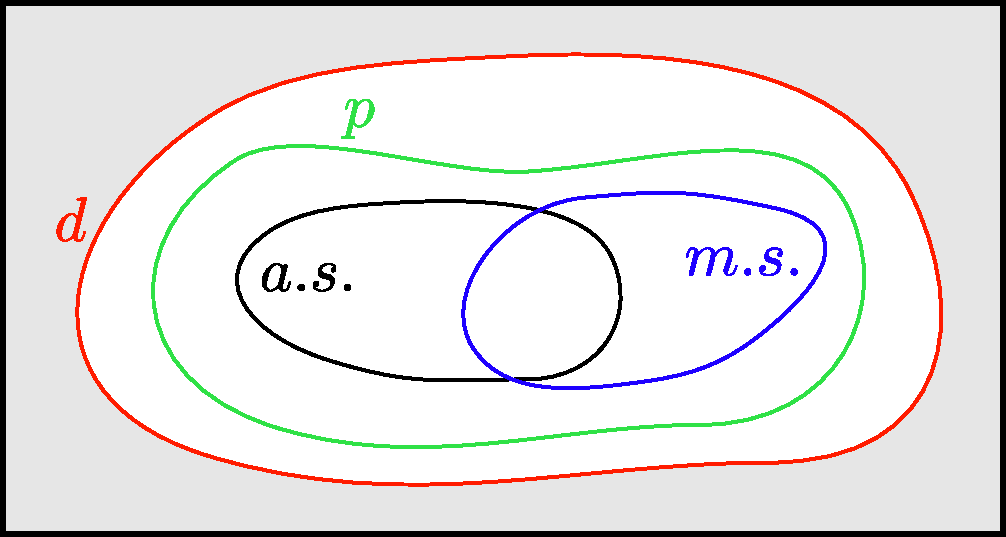
\includegraphics[width=\textwidth]{figuras/convergence_modes_relation.pdf}
  \end{minipage}\hfill
  \begin{minipage}[c]{0.55\textwidth}
    \caption{
       Relación de implicancia de los modos de convergencia. Cada punto del rectángulo representa una secuencia aleatoria. La letra de cada curva indica el modo de convergencia de todas las secuencias dentro de la curva. La parte sombreada contiene las secuencias que no convergen en ningún modo. Tanto convergencia casi segura como convergencia cuadrática media implican convergencia en probabilidad, y convergencia en probabilidad implica convergencia en distribución. Además convergencia casi segura no implica convergencia media cuadrática y viceversa.
    } \label{fig:convergence_modes_relation}
  \end{minipage}
\end{figure}

Previo a la demostración de las implicancias de los modos de convergencia, se dará una explicación intuitiva de la diferencia entre convergencia en probabilidad y  convergencia casi segura, que tienen particular importancia porque son los modos de convergencia que diferencian a la \emph{ley débil de los grandes números} con la \emph{ley fuerte de los grandes números}, como se verá mas adelante. En el esquema de la figura \ref{fig:probability_and_as_convergence} se muestra la diferencia \(|\x_n-\x|\) en función de \(n\). Cada curva representa una realización particular \(|\x_n(\zeta)-\x(\zeta)|\). Convergencia en probabilidad significa que para cierto \(n>n_0\) \emph{específico}, solo un pequeño porcentaje de las curvas tendrá ordenadas que superan \(\epsilon\). Sin embargo, es posible que incluso ninguna de las curvas se mantenga bajo \(\epsilon\) para \emph{todo} \(n>n_0\). Por otro lado, convergencia casi segura requiere que la mayoría de las curvas se mantengan bajo \(\epsilon\) para todo \(n>n_0\). Teniendo en cuenta estas consideraciones, se intuye que convergencia casi segura implica convergencia en probabilidad, y convergencia en probabilidad no implica convergencia casi segura.
\begin{figure}[!htb]
\begin{center}
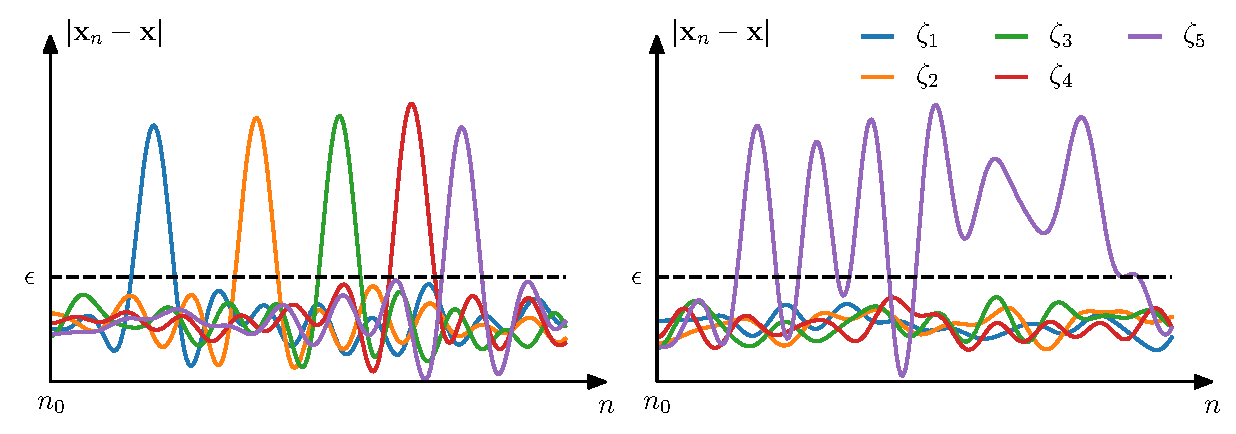
\includegraphics[width=1\columnwidth]{figuras/probability_and_as_convergence.pdf}
\caption{\label{fig:probability_and_as_convergence} Ilustración esquemática de la diferencia de convergencia en probabilidad (izquierda) y convergencia casi segura (derecha). Convergencia en probabilidad implica que para cierto \(n>n_0\) específico, solo un pequeño porcentaje de las curvas \(|\x_n-\x|\) tenga ordenadas que superen \(\epsilon\). En el esquema con cinco realizaciones, solo a lo sumo una curva supera \(\epsilon\) para cada \(n\). Sin embargo, todas las realizaciones superan \(\epsilon\) para algún \(n>n_0\). Convergencia casi segura implica que la mayoría de las curvas no superan \(\epsilon\) para todo \(n>n_0\). En el esquema, solo una realización supera \(\epsilon\), mientras que el resto se mantienen bajo \(\epsilon\) para todo \(n>n_0\).}
\end{center}
\end{figure}


\paragraph{Teorema:} \emph{Convergencia casi segura implica convergencia en probabilidad},
\[
 \x_n\overset{a.s.}{\longrightarrow}\x\qquad\Rightarrow\qquad\x_n\overset{p}{\longrightarrow}\x.
\]
Para demostrarlo, se considera la familia de eventos
\[
  B_n^\epsilon=\{\zeta\in S:\,|\x_n(\zeta)-\x(\zeta)|>\epsilon\},
\]
y por definición, para que \(\x_n\overset{a.s.}{\longrightarrow}\x\), se tiene que cumplir que para todo \(\epsilon>0\), 
\[
 P\{\limsup_{n\to\infty}B_n^\epsilon\}=0.
\]
El lema de Fatou reverso, dado por la ecuación \ref{eq:reverse_fatou_lemma}, indica que
\[
 \limsup_{n\to\infty}P\{B_n^\epsilon\}\leq P\{\limsup_{n\to\infty}B_n^\epsilon\}=0,
\]
y como
\[
 \lim_{n\to\infty}P\{B_n^\epsilon\}\leq\lim_{n\to\infty}\left[\sup_{k\geq n}P\{B_k^\epsilon\}\right]=\limsup_{n\to\infty}P\{B_n^\epsilon\},
\]
se concluye que
\[
 \lim_{n\to\infty}P\{B_n^\epsilon\}=\lim_{n\to\infty}P\{\zeta\in S:\,|\x_n(\zeta)-\x(\zeta)|>\epsilon\}=0,
\]
que es la definición de convergencia en probabilidad, y por lo tanto,
\[
 \x_n\overset{p}{\longrightarrow}\x.
\]

\paragraph{Teorema:} \emph{Convergencia media cuadrática implica convergencia en probabilidad},
\[
 \x_n\overset{m.s.}{\longrightarrow}\x\qquad\Rightarrow\qquad\x_n\overset{p}{\longrightarrow}\x.
\]
Esto es una consecuencia de la desigualdad de Markov. Planteando la desigualdad de Markov, dada por la ecuación \ref{eq:markov_inequality}, para la variable aleatoria \(|\x_n-\x|^2\) y parámetro \(\alpha=\epsilon^2\), se tiene que
\[
 P\{|\x_n-\x|^2>\epsilon^2\}\leq\frac{E\{|\x_n-\x|^2\}}{\epsilon^2},
\]
y como
\[
 P\{|\x_n-\x|^2>\epsilon^2\}=P\{|\x_n-\x|>\epsilon\},
\]
se obtiene que
\[
 P\{|\x_n-\x|>\epsilon\}\leq\frac{E\{|\x_n-\x|^2\}}{\epsilon^2}.
\]
Tomando el límite con \(n\to\infty\), se concluye que
\[
 \lim_{n\to\infty}P\{|\x_n-\x|>\epsilon\}\leq\lim_{n\to\infty}\frac{E\{|\x_n-\x|^2\}}{\epsilon^2}=0,
\]
donde la última igualdad se cumple por hipótesis.

\paragraph{Teorema:} \emph{Convergencia media cuadrática no implica convergencia casi segura}. 

Para demostrarlo, alcanza con encontrar un ejemplo de secuencia aleatoria que converja en media cuadrática pero no converja casi seguramente.
Considérese una familia de variables aleatorias Bernoulli independientes de distribución
\[\def\arraystretch{2.0}
 p_{x_n}(x)=
 \left\{\begin{array}{ll}
  \dfrac{1}{n}, & \x_n=1\\
  1-\dfrac{1}{n}, & \x_n=0
 \end{array}, \right.
\]
y sea \(\x=0\). Se observa primero que \(\x_n\overset{m.s.}{\longrightarrow}\x\), ya que (ver sección \ref{sec:bernoulli_rv_mean_variance})
\[
  E\{|\x_n-\x|^2\}=E\{\x_n^2\}=1^2\times \frac{1}{n}+0^2\times \left(1-\frac{1}{n}\right)=\frac{1}{n}\to0\qquad\textrm{con}\qquad n\to\infty.
\]
Para demostrar que la secuencia no converge casi seguramente, se recurre al segundo lema de Borel-Cantelli (ver sección \ref{sec:independents_events}), que indica que para eventos mutuamente independientes, 
\[
 \textrm{si}\quad \sum_n P(A_n)=\infty\qquad\Rightarrow\qquad P\left(\limsup_n A_n\right) = P(\{A_n\,i.o.\})=1.
\]
En este caso, tomando \(\epsilon=1/2\), se tiene que
\[
 \sum_{n=1}^\infty P\{|\x_n-\x|\geq\epsilon\}=\sum_{n=1}^\infty P\left\{\x_n\geq\frac{1}{2}\right\}
 =\sum_{n=1}^\infty P\left\{\x_n=1\right\}
 =\sum_{n=1}^\infty \frac{1}{n}
 =\infty,
\]
donde en la última igualdad se empleó que la sumatoria es la serie armónica y por lo tanto, diverge\footnote{Ver \url{https://en.wikipedia.org/wiki/Harmonic_series_(mathematics)}}. Cumpliendo las hipótesis del segundo lema de Borel-Cantelli, se tiene que
\[
  \Pr\left(\limsup_{n\to\infty}\left\{|\x_n-\x|>\epsilon \right\}\right)=\Pr\left(\left\{|\x_n-\x|>\epsilon \right\}\;i.o.\right)=1
\]
para cierto valor de \(\epsilon\), concluyendo que \(\x_n\) no converge casi seguramente, como indica la ecuación \ref{eq:almost_sure_convergence_tmp_1}.

Notar además, que la secuencia converge en probabilidad, ya que
\[
 P\{|\x_n-0|>\epsilon\}=P\{\x_n=1\}=\frac{1}{n}\to0\qquad\textrm{con}\qquad n\to\infty,
\]
de lo que se deduce que \emph{convergencia en probabilidad no implica convergencia casi segura}.


\paragraph{Teorema:} \emph{Convergencia casi segura no implica convergencia media cuadrática}. 

Nuevamente, alcanza con encontrar un ejemplo de secuencia aleatoria que converja casi seguramente pero no converja en media cuadrática.
Considérese la familia de variables aleatorias independientes con distribución
\[\def\arraystretch{2.0}
 p_{x_n}(x)=
 \left\{\begin{array}{ll}
  \dfrac{1}{n^2}, & \x_n=n^3\\
  1-\dfrac{1}{n^2}, & \x_n=0
 \end{array}, \right.
\]
y sea \(\x=0\). De esta forma, cuando \(n=10\) por ejemplo, \(\x_n=1000\) con probabilidad \(1/100\), y \(\x_n=0\) con probabilidad \(1-1/100=99/100\).

Se verifica primero que \(\x_n\) no converge en media cuadrática, ya que
\[
  E\{|\x_n-\x|^2\}=E\{\x_n^2\}=n^6\times \frac{1}{n^2}+0^2\times \left(1-\frac{1}{n^2}\right)=n^4\to\infty\qquad\textrm{con}\qquad n\to\infty.
\]
Para demostrar que la secuencia converge casi seguramente, se recurre al lema de Borel-Cantelli (ver sección \ref{sec:probability_measure_continuity}), que indica que 
\[
 \textrm{si}\quad \sum_n P(A_n)<\infty\qquad\Rightarrow\qquad P\left(\limsup_n A_n\right) = P(\{A_n\,i.o.\})=0.
\]
En este caso, para cualquier \(\epsilon>0\), se tiene que\footnote{Ver \url{https://en.wikipedia.org/wiki/Basel_problem}}
\[
 \sum_{n=1}^\infty P\{|\x_n-\x|\geq\epsilon\}=\sum_{n=1}^\infty P\left\{\x_n\geq\epsilon\right\}
 =\sum_{n=1}^\infty P\left\{\x_n=n^3\right\}
 =\sum_{n=1}^\infty \frac{1}{n^2}
 <\infty.
\]
Estando en las hipótesis del lema de Borel-Cantelli, se cumple que
\[
  \Pr\left(\limsup_{n\to\infty}\left\{|\x_n-\x|>\epsilon \right\}\right)=\Pr\left(\left\{|\x_n-\x|>\epsilon \right\}\;i.o.\right)=0,
\]
concluyendo que \(\x_n\) converge casi seguramente, como indica la ecuación \ref{eq:almost_sure_convergence_tmp_2}

Notar además que la secuencia \(\x_n\) converge en probabilidad, ya que
\[
 P\{|\x_n-\x|>\epsilon\}=P\{|\x_n|>\epsilon\}=P\{\x_n=n^3\}=\frac{1}{n^2}\to 0\qquad\textrm{con}\qquad n\to\infty,
\]
lo que indica que \emph{convergencia en probabilidad no implica convergencia en media cuadrática}.

\paragraph{Teorema:} \emph{Convergencia en probabilidad implica convergencia en distribución},
\[
 \x_n\overset{p}{\longrightarrow}\x\qquad\Rightarrow\qquad\x_n\overset{d}{\longrightarrow}\x.
\]

Sean \(a\in\mathbb{R}\) y \(\epsilon>0\). La distribución de probabilidad \(F_{x_n}(a)\) de \(\x_n\) en \(a\) cumple que
\begin{align*}
 F_{x_n}(a)&=P\{\x_n\leq a\}\\
   &\overset{(a)}{=}P\{\x_n\leq a,\,\x\leq a+\epsilon\}+P\{\x_n\leq a,\,\x> a+\epsilon\}\\
   &\overset{(b)}{=}P\{\x_n\leq a\,|\,\x\leq a+\epsilon\}P\{\x\leq a+\epsilon\}+P\{\x_n\leq a,\,a< \x-\epsilon\}\\
   &\overset{(c)}{\leq}P\{\x\leq a+\epsilon\}+P\{\x_n<\x-\epsilon\}\\
   &=F_x(a+\epsilon)+P\{\x-\x_n>\epsilon\}\\
   &\overset{(d)}{\leq}F_x(a+\epsilon)+P\{|\x_n-\x|>\epsilon\},
\end{align*}
donde en \((a)\) se empleó que el evento \(\{\x_n\leq a\}\) se puede expresar como
\begin{align*}
 \{\x_n\leq a\}&=\{\x_n\leq a\}\cap\left(\{\x\leq a+\epsilon\}\cup\{\x> a+\epsilon\}\right)\\
   &=\left(\{\x_n\leq a\}\cap\{\x\leq a+\epsilon\}\right)\cup\left(\{\x_n\leq a\}\cap\{\x> a+\epsilon\}\right),
\end{align*}
y como se trata de la unión de eventos disjuntos, la probabilidad es la suma de las probabilidades, como indica la ecuación \ref{eq:probability_measure_countably_additive}, en \((b)\) se empleó la definición de probabilidad condicional, dada por la ecuación \ref{eq:conditional_probability_definition}, en \((c)\) se empleó que \(P\{\x_n\leq a\,|\,\x\leq a+\epsilon\}\leq1\) y además que
\[
 \textrm{como}\qquad\{\x_n\leq a\}\cap\{a<\x-\epsilon\}\subseteq\{\x_n<\x-\epsilon\}
 \qquad\Rightarrow\qquad
 P(\x_n\leq a,\,a< \x-\epsilon)\leq P(\x_n<\x-\epsilon)
\]
por la propiedad de monotonía de la probabilidad (ecuación \ref{eq:probability_monotony_property}), y en \((d)\) se empleó el mismo argumento notando que
\[
 \{\x-\x_n>\epsilon\}\subseteq\{|\x_n-\x|>\epsilon\}=\{\x_n-\x>\epsilon\}\cup\{\x-\x_n>\epsilon\}.
\]
Por otro lado, empleando un razonamiento análogo, se tiene que
\begin{align*}
 F_x(a-\epsilon)&=P\{\x\leq a-\epsilon\}\\
   &=P\{\x\leq a-\epsilon,\,\x_n\leq a\}+P\{\x\leq a-\epsilon,\,\x_n> a\}\\
   &=P\{\x\leq a-\epsilon\,|\,\x_n\leq a\}P\{\x_n\leq a\}+P\{\x+\epsilon\leq a,\,a<\x_n\}\\
   &\leq P\{\x_n\leq a\}+P\{\x+\epsilon<\x_n\}\\
   &=F_{x_n}(a)+P\{\x_n-\x>\epsilon\}\\
   &\leq F_{x_n}(a)+P\{|\x_n-\x|>\epsilon\}.
\end{align*}
Combinando ambos resultados, se obtiene que
\[
 F_x(a-\epsilon)-P\{|\x_n-\x|>\epsilon\}\leq F_{x_n}(a)\leq F_x(a+\epsilon)+P\{|\x_n-\x|>\epsilon\}.
\]
Tomando el límite cuando \(n\to\infty\), se tiene que
\[
 F_x(a-\epsilon)\leq \lim_{n\to\infty} F_{x_n}(a)\leq F_x(a+\epsilon),
\]
ya que por hipótesis \(\x_n\) converge en probabilidad y por lo tanto \(P\{|\x_n-\x|>\epsilon\}\to 0\) con \(n\to\infty\). También por hipótesis, la distribución \(F_x(x)\) de \(\x\) es continua en \(a\) y por lo tanto \(F_x(a-\epsilon)\) y \(F_x(a+\epsilon)\) tienden a \(F_x(a)\) con \(\epsilon\to0^{+}\). Por lo tanto, al tomar este límite se concluye que
\[
 \lim_{n\to\infty} F_{x_n}(a) = F_x(a),
\]
y por lo tanto \(\x_n\) converge en distribución.

\paragraph{Teorema:} \emph{Convergencia en distribución a una constate implica convergencia en probabilidad a esa constante},
\[
 \x_n\overset{d}{\longrightarrow}c\qquad\Rightarrow\qquad\x_n\overset{p}{\longrightarrow}c.
\]

La variable aleatoria constante \(c\) tiene distribución de probabilidad degenerada\footnote{Ver: \url{https://en.wikipedia.org/wiki/Degenerate_distribution}}
\[\def\arraystretch{1.2}
 F_c(x)=
 \left\{\begin{array}{ll}
  0, &  x<c\\
  1, &  x\geq c
 \end{array}\right.,
\]
y como por hipótesis \(\x_n\overset{d}{\longrightarrow}c\), se debe cumplir que para todo \(\epsilon>0\),
\[
 \lim_{n\to\infty}F_{x_n}(c-\epsilon)=0,\qquad\qquad
 \lim_{n\to\infty}F_{x_n}(c+\epsilon)=1.
\]
Por otro lado, se observa que
\begin{align*}
 \lim_{n\to\infty}P\{|\x_n-c|\geq\epsilon\}&\overset{(a)}{=}\lim_{n\to\infty}\left[P\{\x_n\geq c+\epsilon\}+P\{\x_n\leq c-\epsilon\}\right]\\
 &=\lim_{n\to\infty}P\{\x_n\geq c+\epsilon\}+\lim_{n\to\infty}P\{\x_n\leq c-\epsilon\}\\
 &=\lim_{n\to\infty}\left[1-P\{\x_n< c+\epsilon\}\right]+\lim_{n\to\infty}P\{\x_n\leq c-\epsilon\}\\
 &=1-\lim_{n\to\infty}F_{x_n}(c+\epsilon)+\lim_{n\to\infty}F_{x_n}(c-\epsilon)\\
 &=0,
\end{align*}
donde en \((a)\) se tuvo en cuenta que
\[
 |\x_n-c|\geq\epsilon\quad\Leftrightarrow\quad\{\x_n-c\geq\epsilon\}\cup\{-\x_n+c\geq\epsilon\}
 \quad\Leftrightarrow\quad\{\x_n\geq c+\epsilon\}\cup\{\x_n\leq c-\epsilon\}.
\]
Se concluye que \(\x_n\overset{p}{\longrightarrow}c\).

\paragraph{Ejemplo} Sea \(\x_1,\,\x_2,\,\x_3,\dots\) una secuencia de variables aleatorias independientes e idénticamente distribuidas con distribución uniforme en \((0,\,1)\). Se define la secuencia \(\y_n\) como
\[
 \y_n=\min(\x_1,\dots,\x_n),
\]
y se quiere ver que\footnote{Fuente: \url{https://www.probabilitycourse.com/chapter7/7_2_8_solved_probs.php}.}
\[
 \y_n\overset{d}{\longrightarrow}0,\qquad\qquad \y_n\overset{p}{\longrightarrow}0,\qquad\qquad 
 \y_n\overset{m.s.}{\longrightarrow}0,\qquad\qquad \y_n\overset{a.s.}{\longrightarrow}0.
\]
Se demostrará la convergencia en cada modo de forma independiente sin emplear las relaciones de implicancias.
\begin{itemize}
 \item \emph{Convergencia en distribución: } para ver que la secuencia converge en distribución, se calculará la distribución \(F_{y_n}(y)\) de la variable aleatoria \(\y_n\). Las variables aleatorias \(\x_n\) tienen distribución uniforme en \((0,\,1)\),
\[\def\arraystretch{1.2}
 F_{x_n}(x)=
 \left\{\begin{array}{ll}
  0, & x\leq 0\\
  x, & 0<x< 1\\
  1, & x\geq1
 \end{array}, \right.
\]
por lo tanto, la distribución de \(\y_n\) es
\begin{align*}
 F_{y_n}(y)&=P\{\y_n\leq y\}\\
  &=P\{\min(\x_1,\dots,\x_n)\leq y\}\\
  &=1-P\{\min(\x_1,\dots,\x_n)>y\}\\
  &=1-P\{\x_1>y,\dots,\x_n>y\}\\
  &=1-P\{\x_1>y\}\times\dots\times P\{\x_n>y\},
\end{align*}
donde en la última igualdad se empleo que las variables aleatorias \(\x_n\) son independientes. Continuando con el razonamiento, teniendo en cuenta que \(P\{\x_1>y\}=1-P\{\x_1\leq y\}\), se tiene que
\begin{align*}
 F_{y_n}(y)&=1-(1-P\{\x_1\leq y\})\times\dots\times(1-P\{\x_n\leq y\})\\
  &=1-[1-F_{x_1}(y)]\times\dots\times[1-F_{x_n}(y)]\\
  &=1-(1-y)\times\dots\times(1-y)\\
  &=1-(1-y)^n
\end{align*}
para \(0<y<1\). Teniendo en cuenta además que \(\y_n\in(0,\,1)\), se concluye que
\begin{equation}\label{eq:first_ordered_statistic_distribution}
 \def\arraystretch{1.2}
 F_{y_n}(y)=
 \left\{\begin{array}{ll}
  0, & y\leq 0\\
  1-(1-y)^n, & 0< y <1\\
  1, & y \geq 1
 \end{array}\right..
\end{equation}
Notar que la densidad de probabilidad \(f_{y_n}(y)\) de \(\y_n\) es
\begin{equation}\label{eq:first_ordered_statistic_density}
\def\arraystretch{1.2}
 f_{y_n}(y)=\frac{dF_{y_n}(y)}{dy}=
 \left\{\begin{array}{ll}
  n(1-y)^{n-1}, & 0<y< 1\\
  0, & \textrm{en otro caso}
 \end{array}\right..
\end{equation}
Este resultado ya se había obtenido en la ecuación \ref{eq:ordered_statistic_uniform_density} para la densidad de probabilidad del estadístico de orden 1 de \(n\) variables aleatorias independientes de distribución uniforme. Volviendo al estudio de la convergencia en distribución, para \(0<y<1\) se cumple que \(0<1-y<1\) y por lo tanto
\[
 \lim_{n\to\infty} 1-(1-y)^n=1.
\]
De esta forma, se tiene que
\[\def\arraystretch{1.2}
 \lim_{n\to\infty} F_{y_n}(y)=
 \left\{\begin{array}{ll}
  0, &  y\leq 0\\
  1, & 0< y <1\\
  1, &  y \geq 1
 \end{array}\right.
 =
 \left\{\begin{array}{ll}
  0, &  y \leq 0\\
  1, &  y > 0
 \end{array}\right..
\]
Observando además que la variable aleatoria constante 0 tiene distribución de probabilidad degenerada
\[\def\arraystretch{1.2}
 F_0(y)=
 \left\{\begin{array}{ll}
  0, &  y <0\\
  1, &  y \geq 0
 \end{array}\right.,
\]
se concluye que
\[
 \lim_{n\to\infty} F_{y_n}(y)=F_0(y),\qquad \forall y\in\mathbb{R},\quad y\neq0,
\]
pero el punto \(y=0\) es el único punto de discontinuidad de \(F_0(y)\). En otras palabras, \(F_{y_n}(y)\to F_0(y)\) con \(n\to\infty\) en todo punto donde \(F_0(y)\) es continua, y por lo tanto,
\[
 \y_n\overset{d}{\longrightarrow}0.
\]
\item \emph{Convergencia en probabilidad: } para demostrar que \(\y_n\overset{p}{\longrightarrow}0\) hay que demostrar que
\[
  \lim_{n\to\infty}P\{|\y_n-0|>\epsilon\}=\lim_{n\to\infty}P\{|\y_n|>\epsilon\}=0.
\]
Partiendo de que \(\y_n\in(0,\,1)\), se observa que
\begin{align*}
 P\{|\y_n|>\epsilon\}&=P\{\y_n>\epsilon\}\\
   &=1-P\{\y_n\leq \epsilon\}\\
   &=1-F_{y_n}(\epsilon).
\end{align*}
Para \(\epsilon\in(0,\,1)\), sustituyendo la distribución de probabilidad \(F_{y_n}(\epsilon)\), dada por la ecuación \ref{eq:first_ordered_statistic_distribution}, se obtiene que
\begin{equation}\label{eq:convergence_example_probability}
 P\{|\y_n|>\epsilon\}=(1-\epsilon)^n,
\end{equation}
y por lo tanto,
\[
 \lim_{n\to\infty}P\{|\y_n|>\epsilon\}=\lim_{n\to\infty}(1-\epsilon)^n=0,\qquad\forall\epsilon\in(0,\,1],
\]
que es lo que se quería demostrar.
\item \emph{Convergencia en media cuadrática: } para demostrar que \(\y_n\overset{m.s.}{\longrightarrow}0\) hay que demostrar que
\[
  \lim_{n\to\infty}E\{|\y_n-0|^2\}=\lim_{n\to\infty}E\{\y_n^2\}=0.
\]
Partiendo de la definición de esperanza (ver sección \ref{sec:median_variance_definition}), se tiene que
\begin{align*}
 E\{\y_n^2\}&=\int_{-\infty}^{\infty}y^2f_{y_n}(y)\,dy\\
   &\overset{(a)}{=}n\int_{0}^{1}y^2(1-y)^{n-1}\,dy\\
   &\overset{(b)}{\leq}n\int_{0}^{1}y(1-y)^{n-1}\,dy\\
   &\overset{(c)}{=}-y(1-y)^n\bigg|_0^1+\int_{0}^{1}(1-y)^n\,dy\\
   &=0-\frac{(1-y)^{n+1}}{n+1}\bigg|_0^1\\
   &=\frac{1}{n+1},
\end{align*}
donde en \((a)\) se sustituyó la densidad de probabilidad de \(\y_n\), dada por la ecuación \ref{eq:first_ordered_statistic_density}, en \((b)\) se consideró que \(y^2<y\) para todo \(y\in(0,\,1)\) y en \((c)\) se aplicó integración por partes, \(\int udv=uv-\int vdu\), con \(u=y\) y \(dv=(1-y)^{n-1}\), y entonces \(du=1\) y \(v=-(1-y)^n/n\).
Se concluye que
\[
 \lim_{n\to\infty}E\{|\y_n-0|^2\}\leq\lim_{n\to\infty} \frac{1}{n+1}=0.
\]
\item \emph{Convergencia casi segura: } para demostrar que \(\y_n\overset{a.s.}{\longrightarrow}0\), hay que demostrar que
\[
  P(\{|\y_n-0|\geq\epsilon\}\;i.o.)=0,
\]
y como indica el lema de Borel-Cantelli (ver sección \ref{sec:probability_measure_continuity}), es equivalente a demostrar que
\[
 \sum_{n=1}^\infty P\{|\y_n-0|\geq\epsilon\}<\infty.
\]
Usando el valor de \(P\{|\y_n-0|\geq\epsilon\}\) que ya fue calculado en la ecuación \ref{eq:convergence_example_probability}, se tiene que
\begin{align*}
 \sum_{n=1}^\infty P\{|\y_n-0|\geq\epsilon\}&=\sum_{n=1}^\infty (1-\epsilon)^n\\
   &=\left[\sum_{n=0}^\infty (1-\epsilon)^n\right]-1\\
   &\overset{(a)}{=}\frac{1}{1-(1-\epsilon)}-1\\
   &=\frac{1-\epsilon}{\epsilon}<\infty
\end{align*}
donde en \((a)\) se empleó el resultado de la convergencia de una serie geométrica, dado en la ecuación \ref{eq:geometric_series_convergence}.
\end{itemize}

\subsection{La ley de los grandes números}\label{sec:lln}

La \emph{ley de los grandes números} (LLN, \emph{law of large numbers}) describe el resultado al realizar el mismo experimento reiteradas veces. De acuerdo a la ley, el promedio de los resultados en una cantidad grande de ensayos se aproxima al valor esperado teórico del experimento, y la aproximación es mejor a medida que se incrementa la cantidad de ensayos. Hay dos versiones de la ley, la \emph{débil} y la \emph{fuerte}. La versión débil indica que la convergencia del promedio al valor esperado es en probabilidad, y la versión fuerte indica que la convergencia es casi segura. 
La primera demostración de la ley débil de los grandes números fue realizada por Jacob Bernoulli en 1713 para variables aleatorias binarias. En 1907, Émile Borel formuló y demostró la versión fuerte de la ley.

Se comenzará con la ley en el caso particular de ensayos de Bernoulli, que es la que se incluye en \cite{papoulis2002probability}, y luego se planteará la forma general de la ley.

\subsubsection{La ley débil de los grandes números (Bernoulli)}

En la sección \ref{sec:bernoulli_theorem} se demostró el teorema de Bernoulli, que indica que si la probabilidad de ocurrencia de cierto evento \(A\) en un experimento es \(p\) y el número de ocurrencias de \(A\) en \(n\) ensayos es \(k\), se cumple que (ecuación \ref{eq:bernoulli_theorem}),
\[
 P\left\{\left|\frac{k}{n}-p\right|<\epsilon\right\}>1-\frac{pq}{n\epsilon^2},
\]
y por lo tanto,
\begin{equation}\label{eq:bernoulli_theorem_2}
 P\left\{\left|\frac{k}{n}-p\right|<\epsilon\right\}\to1,\qquad\textrm{con}\qquad n\to\infty.
\end{equation}
Se demostrará nuevamente este resultado como el límite de una secuencia de variables aleatorias. Para esto, se definen las variables aleatorias
\[\def\arraystretch{1.2}
 \x_i=
 \left\{\begin{array}{ll}
  1, &  \textrm{si }A\textrm{ ocurre en el }i\textrm{-ésimo ensayo}\\
  0, &  \textrm{en otro caso},
 \end{array}\right.
\]
y se demostrará que la media muestral,
\[
 \bar{\x}_n=\frac{\x_1+\dots+\x_n}{n}
\]
converge a \(p\) en probabilidad cuando \(n\to\infty\). Para hacerlo, se empleará la desigualdad de Chebyshev, dada por la ecuación \ref{eq:chebyshev_inequality}, que indica que
\[
 P\{|\bar{\x}_n-\eta_{x_n}|<\epsilon\}\geq 1-\frac{\sigma^2_{x_n}}{\epsilon^2}.
\]
En este caso, \(\eta_{x_i}=p\) y \(\sigma^2_{x_i}=pq\), como se dedujo en la sección \ref{sec:bernoulli_rv_mean_variance}, y por lo tanto,
\[
 \eta_{x_n}\overset{(a)}{=}\frac{n\eta_{x_i}}{n}=\eta_{x_i}=p\qquad\qquad\textrm{y}\qquad\qquad
 \sigma^2_{x_n}\overset{(b)}{=}\frac{n\sigma^2_{x_i}}{n^2}=\frac{\sigma^2_{x_i}}{n}=\frac{pq}{n},
\]
donde en \((a)\) se empleó la propiedad de linealidad de la esperanza y en \((b)\) que la varianza de la suma de variables aleatorias independientes es la suma de las varianzas (ver ecuación \ref{eq:sum_of_rv_variance}) y además que la multiplicación de una variable aleatoria por una constante incrementa a la varianza como el cuadrado de la constante (ecuación \ref{eq:variance_linear_transform}). Sustituyendo estos resultados en la desigualdad de Chebyshev, se obtiene que
\[
 P\{|\bar{\x}_n-p|<\epsilon\}\geq 1-\frac{pq}{n\epsilon^2}.
\]
Observando además que \(pq=p(1-p)\leq1/4\), ya que se trata de un polinomio de segundo grado en \(p\) de concavidad negativa cuyo valor máximo se da en \(p=1/2\) y es \(1/4\), se cumple que
\[
 P\{|\bar{\x}_n-p|<\epsilon\}\geq 1-\frac{pq}{n\epsilon^2}\geq1-\frac{1}{4n\epsilon^2}\to1\qquad\textrm{con}\qquad n\to\infty,
\]
es decir,
\[
 \bar{\x}_n\overset{p}{\longrightarrow}p.
\]
Además, si el evento \(A\) ocurre \(k\) veces se cumple que \(\bar{\x}_n=k/n\), obteniendo la ecuación \ref{eq:bernoulli_theorem_2}.

\subsubsection{La ley fuerte de los grandes números (Borel)}

La versión fuerte de ley indica que \(\bar{\x}_n\) converge a \(p\) no solo en probabilidad, sino también casi seguramente o con probabilidad 1. La demostración de este resultado es difícil y no se incluirá. Se realiza a continuación una interpretación de la diferencia de implicancias entre la ley débil y la ley fuerte en términos de la frecuencia relativa.

Supóngase que cierto evento tiene una probabilidad de ocurrencia \(p\), y se pretende estimar \(p\) con un error menor a \(\epsilon=0.1\). Para eso, se repite el experimento \(n=1000\) veces y se usa como estimador la media muestral \(\bar{\x}_n\). De esta forma, se cumple que
\[
 P\{|\bar{\x}_n-p|<\epsilon\}\geq1-\frac{1}{4n\epsilon^2}=1-\frac{1}{4\times1000\times0.01}=1-\frac{1}{40}=\frac{39}{40}.
\]
Este resultado indica que en 39 cada 40 realizaciones \(\zeta_i\) de \(\bar{\x}_{1000}(\zeta_i)\), el error \(|\bar{\x}_{1000}(\zeta_i)-p|\) será menor que \(0.1\).

Supóngase ahora que el experimento se repite \(n=2000\) veces, y se determina la media muestral \(\bar{\x}_n\) no solo para un valor de \(n\), sino para todo \(n\) entre 1000 y 2000. La ley débil de los grandes números permite concluir lo siguiente: si se realiza el experimento \(\zeta_i\) con \(n=2000\) una cantidad \(i\) grande de veces, se cumple que para un valor específico de \(n\geq 1000\), el error \(|\bar{\x}_n(\zeta_i)-p|\) será mayor que \(0.1\) una de cada 40 realizaciones \(\zeta_i\). En otras palabras, el 97.5\% de las realizaciones serán ``buenas'' en el sentido en que el error será menor que \(\epsilon\) para ese \(n\) específico. 
Lo que la lay débil no permite concluir es que en esas buenas realizaciones el error se mantenga menor que \(\epsilon\) para todo \(n\) entre 1000 y 2000. Esto último sin embargo es cierto, pero  solo se puede concluir a partir de la ley fuerte de los grandes números.

\subsubsection{La ley débil de los grandes números (Khinchin, caso general)}

Sea \(\x_1,\,\x_2,\dots\) una secuencia de variables aleatorias i.i.d. con valor esperado finito \(\eta\), es decir,
\[
 E\{\x_1\}=E\{\x_2\}=\dots=\eta<\infty,
\]
y sea la media muestral,
\[
 \bar{\x}_n=\frac{\x_1+\dots+\x_n}{n}.
\]
La ley débil de los grandes números indica que
\[
 \bar{\x}_n\overset{p}{\longrightarrow}\eta.
\]
La demostración puede realizarse a partir de la inecuación de Chebyshev de forma idéntica al caso de variables aleatorias binarias visto previamente\footnote{ver \url{https://en.wikipedia.org/wiki/Law_of_large_numbers}, por ejemplo.}. Se incluye a continuación otra demostración empleando las funciones características, que tiene interés por la similitud a la demostración del teorema central del límite, el que se verá mas adelante. La demostración desarrollada a contiuación está basada en \cite{polyanskiy18lec17}.

Para la prueba, se tendrán en cuenta las siguientes tres consideraciones:
\begin{enumerate}
 \item \emph{Desarrollo de Taylor de primer orden}: sea \(g:\mathbb{R}\to\mathbb{R}\) una función que tiene derivada en cero, y sea la expansión de Taylor de primer orden en torno a cero
 \[
  g(x)=g(0)+g'(0)x+h(x),
 \]
 donde \(h(x)\) representa el error en la aproximación de primer orden. Por definición de la derivada, se cumple que
 \[
  g'(0)=\lim_{x\to0}\frac{g(x)-g(0)}{x}=\lim_{x\to0}\frac{g'(0)x+h(x)}{x}=g'(0)+\lim_{x\to0}\frac{h(x)}{x},
 \]
 resultando en que
 \[
  \lim_{x\to0}\frac{h(x)}{x}=0.
 \]
 Una función \(h\) con esta propiedad se denota \(o(x)\)\footnote{ver \url{https://en.wikipedia.org/wiki/Big_O_notation\#Little-o_notation}, por ejemplo}. Estas observaciones también son válidas para funciones complejas considerando separadamente la parte real y la parte imaginaria.
 \item \emph{Función exponencial}: recordar el hecho bien conocido de que
 \[
  \lim_{n\to\infty}\left(1+\frac{a}{n}\right)^n=e^a,\qquad a\in\mathbb{R}.
 \]
 La identidad se cumple además en el caso en que \(a\) es un número complejo. Adicionalmente, se puede probar que si \(\{a_n\}\) es una secuencia de números complejos que converge a \(a\), se cumple que
 \[
  \lim_{n\to\infty}\left(1+\frac{a_n}{n}\right)^n=e^a.
 \]
 \item \emph{Teorema de continuidad de Levy}. El teorema de continuidad de Levy o de convergencia de Levy vincula la convergencia en distribución de una secuencia de variables aleatorias con la convergencia puntual de sus funciones características. A continuación se incluye su formulación, pero no se demostrará.
 \begin{itemize}
  \item[] Sea \(\x_n\) una secuencia de variables aleatorias con distribuciones de probabilidad \(F_n(x)\) y funciones características \(\Phi_n(\omega)\). Sea \(\x\) una variable aleatoria con distribución de probabilidad \(F(x)\) y función característica \(\Phi(\omega)\). Si se cumple que
  \[
   \Phi_n(\omega)\to\Phi(\omega)\qquad\forall \omega\in\mathbb{R},
  \]
  es decir, la secuencia \(\Phi_n(\omega)\) de funciones características converge puntualmente a \(\Phi(\omega)\), se cumple que 
  \[
   F_n(x)\to F(x)
  \]
 en todos los puntos de continuidad de \(F(x)\). En otras palabras, \(\x_n\) converge en distribución a \(\x\),
 \[
  \x_n\overset{d}{\to}\x.
 \]
 \end{itemize}
\end{enumerate}
Se parte considerando un desarrollo de Taylor de primer orden de la función característica.
Teniendo en cuenta que la función característica de una variable aleatoria \(\x\) cumple que
\[
 \begin{array}{ccccccccccc}
  \Phi_x(\omega)&=&E(e^{j\omega\x})&\qquad&\Rightarrow&\qquad&\Phi_x(0)&=&E(1)&=&1\\
  \Phi'_x(\omega)&=&jE(\x e^{j\omega\x})&\qquad&\Rightarrow&\qquad&\Phi'_x(0)&=&jE(\x)&=&j\eta,
 \end{array}
\]
el desarrollo de Taylor de primer orden en torno a cero es
\[
 \Phi_x(\omega)=1+j\eta\omega+o(\omega),\qquad\omega\to0.
\]
Como las variables aleatorias \(\x_1,\,\x_2,\dots\) son i.i.d., todas tienen la misma función característica, que se denotará \(\Phi_x(\omega)\).
Considerando las siguientes propiedades de la función característica,
\[
 \Phi_\frac{x}{n}(\omega)=\Phi_x\left(\frac{\omega}{n}\right)
 \qquad\textrm{y}\qquad
 \Phi_{x+y}(\omega)=\Phi_x(\omega)\Phi_y(\omega)
\]
si \(\x\) y \(\y\) son independientes (ver las ecuaciones \ref{eq:characteristic_function_of_linear_function_of_rv} y \ref{eq:characteristic_function_convolution_theorem}), la función característica de \(\bar{\x}_n\) se puede expresar en términos de \(\Phi_x(\omega)\) como
\[
 \Phi_{\bar{x}_n}(\omega)=\left[\Phi_x\left(\frac{\omega}{n}\right)\right]^n=\left[1+j\frac{\eta\omega}{n}+o\left(\frac{\omega}{n}\right)\right]^n,
\]
donde en la segunda igualdad se empleó el desarrollo de Taylor de primer orden considerado previamente, con la función \(o\) cumpliendo que \(\lim_{x\to0}o(x)/x=0\). Tomando el límite \(n\to\infty\) se obtiene que
\[
 \lim_{n\to\infty}\Phi_{\bar{x}_n}(\omega)=e^{j\eta\omega},\qquad\forall\omega.
\]
\(e^{j\eta\omega}\) se reconoce como la función característica de una variable aleatoria degenerada que toma el valor \(\eta\) con probabilidad uno. Esto es porque la densidad de probabilidad de una variable aleatoria constante que toma el valor \(\eta\) es \(\delta(x-\eta)\), por lo que la función característica es
\[
 \Phi(\omega)=\int_{-\infty}^\infty\delta(x-\eta) e^{j\omega x}\,dx=e^{j\eta\omega}.
\]
Aplicando el teorema de continuidad de Levy, se obtiene que 
\[
 \x_n\overset{d}{\to}\eta.
\]
Pero como convergencia en distribución a una constante implica convergencia en probabilidad, como se mostró en la sección \ref{sec:convergence_modes}, se concluye que 
\[
 \x_n\overset{p}{\to}\eta.
\]

A continuación se incluyen los llamados \emph{teorema de Markov} y \emph{condición de Chebyshev} en \cite{papoulis2002probability}. Sin embargo, no se encontró otra referencia a los teoremas con dichos nombres en la bibliografía.

\subsubsection{Teorema de Markov}

A partir de una secuencia de \(\x_i\) de variables aleatorias, se construye su media muestral
\[
 \bar{\x}_n=\frac{\x_1+\dots+\x_n}{n}.
\]
De esta forma, \(\bar{\x}_n\) es una variable aleatoria cuyos valores \(\bar{\x}_n(\zeta)\) dependen del resultado \(\zeta\) del experimento. Se demostrará que si las variables aleatorias \(\x_i\) son tales que la media \(\bar{\eta}_n\) de \(\bar{\x}_n\) tiende a un límite \(\eta\) y su varianza tiende a 0 con \(n\to\infty\), es decir,
\[
 E\{\bar{\x}_n\}=\bar{\eta}_n\xrightarrow[n\to\infty]{}\eta
  \qquad\qquad\textrm{y}\qquad\qquad
 \bar{\sigma}_n^2=E\{(\bar{\x}_n-\bar{\eta}_n)^2\}\xrightarrow[n\to\infty]{}0, 
\]
se cumple que la variable aleatoria \(\bar{\x}_n\) tiende a \(\eta\) en el sentido cuadrático medio,
\[
 E\{(\bar{\x}_n-\eta)^2\}\xrightarrow[n\to\infty]{}0
 \qquad\qquad\textrm{o}\qquad\qquad
 \bar{\x}_n\xrightarrow[]{m.s.}\eta
\]
La demostración se basa en la desigualdad
\[
 |\bar{\x}_n-\eta|^2\leq2|\bar{\x}_n-\bar{\eta}_n|^2+2|\bar{\eta}_n-\eta|^2.
\]
Esta desigualdad proviene de que por un lado
\[
 |\bar{\x}_n-\eta|=|\bar{\x}_n-\bar{\eta}_n+\bar{\eta}_n-\eta|\leq|\bar{\x}_n-\bar{\eta}_n|+|\bar{\eta}_n-\eta|,
\]
donde la desigualdad proviene de aplicar la desigualdad triangular. Por lo tanto,
\[
 |\bar{\x}_n-\eta|^2\leq(|\bar{\x}_n-\bar{\eta}_n|+|\bar{\eta}_n-\eta|)^2=|\bar{\x}_n-\bar{\eta}_n|^2+|\bar{\eta}_n-\eta|^2+2|\bar{\x}_n-\bar{\eta}_n||\bar{\eta}_n-\eta|.
\]
Por otro lado, se cumple que
\[
 (|\bar{\x}_n-\bar{\eta}_n|-|\bar{\eta}_n-\eta|)^2=|\bar{\x}_n-\bar{\eta}_n|^2+|\bar{\eta}_n-\eta|^2-2|\bar{\x}_n-\bar{\eta}_n||\bar{\eta}_n-\eta|\geq0,
\]
es decir,
\[
 2|\bar{\x}_n-\bar{\eta}_n||\bar{\eta}_n-\eta|\leq|\bar{\x}_n-\bar{\eta}_n|^2+|\bar{\eta}_n-\eta|^2.
\]
Combinando ambos resultados, se obtiene que
\[
 |\bar{\x}_n-\eta|^2\leq|\bar{\x}_n-\bar{\eta}_n|^2+|\bar{\eta}_n-\eta|^2+2|\bar{\x}_n-\bar{\eta}_n||\bar{\eta}_n-\eta|\leq2|\bar{\x}_n-\bar{\eta}_n|^2+2|\bar{\eta}_n-\eta|^2,
\]
que es la desigualdad que se empleará. Tomando los valores esperados en ambos lados resulta en
\[
 E\{(\bar{\x}_n-\eta)^2\}\leq2E\{(\bar{\x}_n-\bar{\eta}_n)^2\}+2(\bar{\eta}_n-\eta)^2\xrightarrow[n\to\infty]{}0,
\]
donde la convergencia a 0 es por las hipótesis. 

\paragraph{Corolario: condición de Tchebycheff} Si las variables aleatorias \(\x_i\) son no correlacionadas y además
\begin{equation}\label{eq:chebyshev_condition}
 \frac{\sigma^2_1+\dots+\sigma^2_n}{n^2}\xrightarrow[n\to\infty]{}0,
\end{equation}
se cumple que 
\[
 \x_n\xrightarrow[]{m.s.}\eta=\lim_{n\to\infty}\frac{1}{n}\sum_{i=1}^nE\{\x_i\}.
\]
Esto es una consecuencia del teorema de Markov, ya que como las variables aleatorias \(\x_i\) son no correlacionadas, el lado izquierdo de la ecuación \ref{eq:chebyshev_condition} es \(\bar{\sigma}^2_n\). La ecuación \ref{eq:chebyshev_condition} es la condición de Tchebycheff, y es satisfecha si \(\sigma_i<K<\infty\) para todo \(i\). Ese es el caso si las variables aleatorias \(\x_i\) son i.i.d. y de varianza finita.

\subsection{Teorema central del límite}

La suma de \(n\) variables aleatorias \(\x_i\) independientes,
\[
 \x=\x_1+\dots+\x_n,
\]
es una variable aleatoria con media y varianza
\begin{equation}\label{eq:clt_mean_and_variance}
 \eta=\eta_1+\dots+\eta_n\qquad\qquad\textrm{y}\qquad\qquad\sigma^2=\sigma^2_1+\dots+\sigma^2_n
\end{equation}
respectivamente. El teorema central del límite (CLT, \emph{central limit theorem}) establece que en ciertas condiciones generales, la distribución \(F(x)\) de \(\x\) se aproxima a una distribución normal con la misma media y varianza a medida que \(n\) crece, es decir,
\[
 F(x)\approx G\left(\frac{x-\eta}{\sigma}\right),
\]
donde \(G(x)\) es la distribución normal de media nula y varianza unidad.
Adicionalmente, si las variables aleatorias \(\x_i\) son continuas, la densidad \(f(x)\) de \(\x\) se aproxima a una densidad normal,
\begin{equation}\label{eq:central_limit_theorem_density}
 f(x)\approx\frac{1}{\sqrt{2\pi\sigma^2}}e^{-(x-\eta)^2/2\sigma^2}.
\end{equation}
El teorema puede ser formulado como un límite. Si \(\z=(\x-\eta)/\sigma\), se cumple que 
\[
 F_z(z)\xrightarrow[n\to\infty]{}G(z)
 \qquad\qquad\textrm{o}\qquad\qquad
 f_z(z)\xrightarrow[n\to\infty]{}\frac{1}{\sqrt{2\pi}}e^{-z^2/2}
\]
para el caso general y el caso continuo respectivamente.

El CLT es consecuencia de una propiedad del producto convolución: la convolución de una cantidad grande de funciones positivas (ver la ecuación \ref{eq:densities_convolution_random_vector}) tiende a una función normal. El siguiente ejemplo es una ilustración de esto.

\paragraph{Ejemplo 7-15}\label{sec:example_7_15} Sean la variables \(\x_i\) i.i.d. con distribución uniforme en el intervalo \((0,\,T)\). Se comparará la densidad \(f_n(x)\) de su suma con la densidad normal para el caso \(n=2\) y \(n=3\). Es fácil ver que la media es \(\eta_i=T/2\) y la varianza es
\begin{align*}
 \sigma^2_i&=\int_{-\infty}^\infty(x-\eta_i)^2f(x)\,dx\\
  &\overset{(a)}{=}\frac{1}{T}\int_{0}^{T}\left(x-\frac{T}{2}\right)^2\,dx\\
  &\overset{(b)}{=}\frac{1}{T}\int_{-T/2}^{T/2}u^2\,du\\
  &=\frac{1}{T}\frac{u^3}{3}\bigg|_{-T/2}^{T/2}\\
  &=\frac{1}{T}\left(\frac{T^3}{24}+\frac{T^3}{24}\right)\\
  &=\frac{T^2}{12}
\end{align*}
donde en \((a)\) se consideró que \(f(x)=1/T\) en \((0,\,T)\) y 0 en otro caso, y en \((b)\) se realizó el cambio de variable \(u=x-T/2\). Por lo tanto, en este problema se tiene que (ver la ecuación \ref{eq:clt_mean_and_variance})
\[
 \eta_i=\frac{T}{2},\qquad\sigma_i^2=\frac{T^2}{12},\qquad\eta_n=n\frac{T}{2},\qquad\sigma_n^2=n\frac{T^2}{12}.
\]
De la ecuación \ref{eq:pdf_of_sum_of_two_independents_rv}, la densidad de la suma de variables aleatorias i.i.d. es la convolución de las densidades.
\begin{itemize}
 \item Caso \(n=2\): la densidad es
\[
 f_2(x)=\int_{-\infty}^{\infty}f_1(y)f_1(x-y)\,dy,
\]
y se distinguen los siguientes casos (ver la figura \ref{fig:joint_distribution_sum_sub_marginals_convolutions}):
 \begin{itemize}
  \item \(0\leq x\leq T\):
  \[
   f_2(x)=\int_{0}^x\frac{1}{T^2}\,dy=\frac{1}{T^2}y\bigg|_{0}^x=\frac{x}{T^2}
  \]
  \item \(T\leq x\leq 2T\):
  \[
   f_2(x)=\int_{x-T}^T\frac{1}{T^2}\,dy=\frac{1}{T^2}y\bigg|_{x-T}^T=\frac{1}{T^2}[T-(x-T)]=\frac{-x+2T}{T^2}.
  \]
 \end{itemize}
 Se concluye que
 \[
 f_2(x)=
\def\arraystretch{2}\arraycolsep=9pt
 \left\{\begin{array}{ll}
   \displaystyle\frac{x}{T^2}, &  0\leq x\leq T\\
   \displaystyle\frac{-x+2T}{T^2}, & T\leq x\leq 2T\\ 
   0 & \textrm{en otro caso.}
 \end{array} \right.
\]
\item Caso \(n=3\): la densidad es
\[
 f_3(x)=\int_{-\infty}^{\infty}f_2(y)f_1(x-y)\,dy,
\]
 y se distinguen los siguientes casos:
 \begin{itemize}
  \item \(0\leq x\leq T\):
  \[
   f_3(x)=\int_{0}^x\frac{y}{T^2}\times\frac{1}{T}\,dy=\frac{1}{T^3}\times\frac{y^2}{2}\bigg|_{0}^x=\frac{x^2}{2T^3}
  \]
  \item \(T\leq x\leq 2T\):
  \begin{align*}
   f_3(x)&=\int_{x-T}^T\frac{y}{T^2}\times\frac{1}{T}\,dy+\int_{T}^x\frac{-y+2T}{T^2}\times\frac{1}{T}\,dy\\
   &=\frac{y^2}{2T^3}\bigg|_{x-T}^T+\frac{1}{T^3}\left(-\frac{y^2}{2}+2Ty\right)\bigg|_{T}^x\\
   &=\frac{1}{2T^3}\left[T^2-(x-T)^2\right]+\frac{1}{T^3}\left[\left(-\frac{x^2}{2}+2Tx\right)-\left(-\frac{T^2}{2}+2T^2\right)\right]\\
   &=\frac{1}{2T^3}\left[\left(-x^2+2Tx\right)+\left(-x^2+4Tx-3T^2\right)\right]\\
   &=\frac{1}{2T^3}\left(-2x^2+6Tx-3T^2\right)
  \end{align*}
  \item \(2T\leq x\leq 3T\):
  \begin{align*}
   f_3(x)&=\int_{x-T}^{2T}\frac{-y+2T}{T^2}\times\frac{1}{T}\,dy\\
   &=\frac{1}{T^3}\left(-\frac{y^2}{2}+2Ty\right)\bigg|_{x-T}^{2T}\\
   &=\frac{1}{T^3}\left\{\left[-\frac{4T^2}{2}+4T^2\right]-\left[-\frac{(x-T)^2}{2}+2T(x-T)\right]\right\}\\
   &=\frac{1}{2T^3}\left\{4T^2-\left[(-x^2+2Tx-T^2)+(4Tx-4T^2)\right]\right\}\\
   &=\frac{1}{2T^3}\left(x^2-6Tx+9T^2\right)
  \end{align*}
 \end{itemize}
 resultando en
\begin{equation}\label{eq:example_7_15_density_of_sum}
  f_3(x)=
\def\arraystretch{2}\arraycolsep=9pt
 \left\{\begin{array}{ll}
   \displaystyle\frac{x^2}{2T^3}, &  0\leq x\leq T\\
   \displaystyle\frac{1}{2T^3}\left(-2x^2+6Tx-3T^2\right), & T\leq x\leq 2T\\ 
   \displaystyle\frac{1}{2T^3}\left(x^2-6Tx+9T^2\right), & 2T\leq x\leq3T\\ 
   0 & \textrm{en otro caso.}
 \end{array} \right.
\end{equation}
\end{itemize}
\begin{figure}[!htb]
\begin{center}
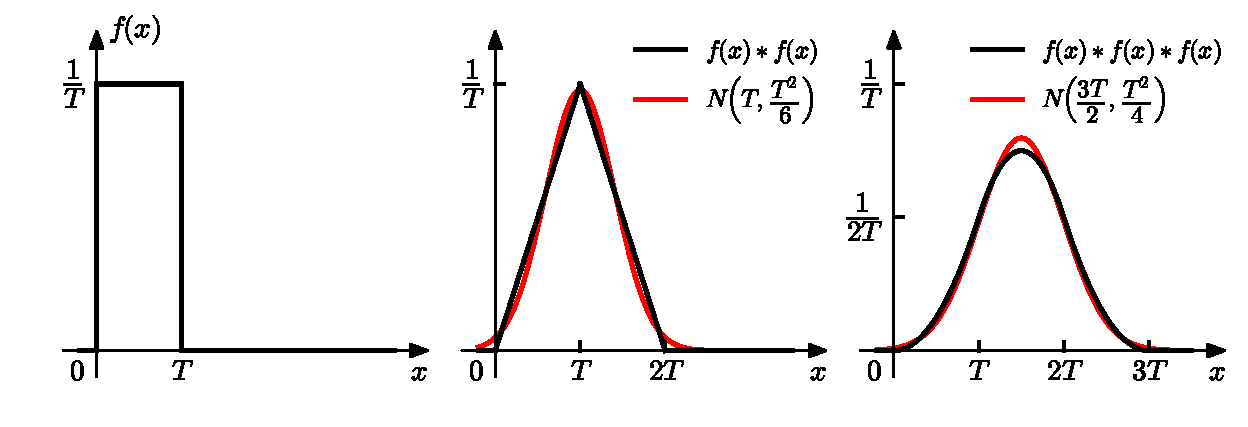
\includegraphics[width=0.95\columnwidth]{figuras/example_7_15.pdf}
\caption{\label{fig:example_7_15} Ilustración del teorema central del límite. Se comparan las densidades de \(\x_1+\x_2\) y \(\x_1+\x_2+\x_3\), donde \(\x_i\sim U(0,\,T)\), con las correspondientes aproximaciones gaussianas.}
\end{center}
\end{figure}
En la figura \ref{fig:example_7_15} se muestra la comparación de las densidades \(f_2(x)\) y \(f_3(x)\) de las variables aleatorias \(\x_1+\x_2\) y \(\x_1+\x_2+\x_3\) respectivamente con su correspondiente aproximación gaussiana, \(N(T,\,T^2/6)\) y \(N(3T/2,\,T^2/4)\). Como se aprecia en la figura, el error es pequeño incluso para los valores chicos de \(n\) empleados.

\subsubsection{Corrección del error}

En la aproximación de \(f(x)\) por una curva normal \(N(\eta,\,\sigma^2)\), el error es
\begin{equation}\label{eq:hermite_error_correction}
 \epsilon(x)=f(x)-\frac{1}{\sqrt{2\pi\sigma^2}}e^{-x^2/2\sigma^2},
\end{equation}
donde sin perder generalidad se asumió que \(\eta=0\), lo que implica únicamente desplazar el origen de coordenadas. Se verá que este error se puede expresar en función de los momentos
\[
 m_n=E\{\x^n\}
\]
de \(\x\) y los polinomios de Hermite \cite{singer2006moment}, que se definen como
\begin{equation}\label{eq:hermite_polinomials}
 H_k(x)=(-1)^ke^{x^2/2}\frac{d^k}{dx^k}e^{-x^2/2}. 
\end{equation}
Estos polinomios forman una base ortogonal en el eje real respecto a la función de ponderación \(e^{-x^2/2}\),
\[
 \frac{1}{\sqrt{2\pi}}\int_{-\infty}^{\infty}e^{-x^2/2}H_n(x)H_m(x)\,dx=
 \left\{\begin{array}{ll}
  n! & n=m \\
  0 & n\neq m,
 \end{array} \right.
\]
o cambiando la variable \(x\) por \(x/\sigma\),
\begin{equation}\label{eq:hermite_orthogonality}
 \frac{1}{\sqrt{2\pi\sigma^2}}\int_{-\infty}^{\infty}e^{-x^2/2\sigma^2}H_n\left(\frac{x}{\sigma}\right)H_m\left(\frac{x}{\sigma}\right)\,dx=
 \left\{\begin{array}{ll}
  n! & n=m \\
  0 & n\neq m.
 \end{array} \right. 
\end{equation}
Empleando la base de polinomios de Hermite, la densidad de probabilidad \(f(x)\) puede escribirse como la serie
\begin{equation}\label{eq:hermite_density_expansion}
 f(x)=\frac{1}{\sqrt{2\pi\sigma^2}}e^{-x^2/2\sigma^2}\sum_{k=0}^\infty C_kH_k\left(\frac{x}{\sigma}\right).
\end{equation}
Para encontrar los coeficientes \(C_n\), se multiplica ambos lados de la igualdad por \(H_n(x/\sigma)\) y se integra,
\[
 \int_{-\infty}^\infty f(x)H_n\left(\frac{x}{\sigma}\right)\,dx=\sum_{k=0}^\infty C_k\left[\frac{1}{\sqrt{2\pi\sigma^2}}\int_{-\infty}^\infty e^{-x^2/2\sigma^2}H_k\left(\frac{x}{\sigma}\right)H_n\left(\frac{x}{\sigma}\right)\,dx\right].
\]
Observando que el lado izquierdo de la igualdad es la esperanza de \(H_n(x/\sigma)\) y empleando la ecuación \ref{eq:hermite_orthogonality} en el lado derecho, se obtiene que 
\begin{equation}\label{eq:hermite_expansion_coefficients}
 E\left\{H_n\left(\frac{x}{\sigma}\right)\right\}=C_nn!
\qquad\qquad\Rightarrow\qquad\qquad
 C_n=\frac{1}{n!}E\left\{H_n\left(\frac{x}{\sigma}\right)\right\}.
\end{equation}
Se verá ahora que los coeficientes \(C_n\) pueden expresarse en función de los momentos \(m_n\) de \(\x\). Para hacerlo, se calculará \(H_n(x)\) para \(n=0,\,\dots,\,4\) con la ecuación \ref{eq:hermite_polinomials}. Primero se parte observando que
\begin{align*}
 \frac{d^0}{dx^0}e^{-x^2/2}&=e^{-x^2/2}\\
 \frac{d}{dx}\;e^{-x^2/2}&=-\frac{2x}{2}e^{-x^2/2}=-xe^{-x^2/2}\\
 \frac{d^2}{dx^2}e^{-x^2/2}&=-e^{-x^2/2}-x(-xe^{-x^2/2})=(x^2-1)e^{-x^2/2}\\
 \frac{d^3}{dx^3}e^{-x^2/2}&=2xe^{-x^2/2}+(x^2-1)(-xe^{-x^2/2})=(-x^3+3x)e^{-x^2/2}\\
 \frac{d^4}{dx^4}e^{-x^2/2}&=(-3x^2+3)e^{-x^2/2}+(-x^3+3x)(-xe^{-x^2/2})=(x^4-6x^2+3)e^{-x^2/2},
\end{align*}
y sustituyendo estos resultados en la ecuación \ref{eq:hermite_polinomials} se obtiene que 
\[
 H_0(x)=1,\qquad H_1(x)=x,\qquad H_2(x)=x^2-1,\qquad H_3(x)=x^3-3x,\qquad H_4(x)=x^4-6x^2+3.
\]
Finalmente, la ecuación \ref{eq:hermite_expansion_coefficients} conduce a que los coeficientes son
\begin{align*}
 C_0&=E\left\{H_0\left(\frac{x}{\sigma}\right)\right\}=1\\
 C_1&=E\left\{H_1\left(\frac{x}{\sigma}\right)\right\}=E\left\{\frac{x}{\sigma}\right\}=\frac{\eta}{\sigma}=0\\
 C_2&=\frac{1}{2!}E\left\{H_2\left(\frac{x}{\sigma}\right)\right\}=\frac{1}{2}E\left\{\frac{x^2}{\sigma^2}-1\right\}=\frac{1}{2}\left(\frac{\sigma^2}{\sigma^2}-1\right)=0\\
 C_3&=\frac{1}{3!}E\left\{H_3\left(\frac{x}{\sigma}\right)\right\}=\frac{1}{6}E\left\{\frac{x^3}{\sigma^3}-\frac{3x}{\sigma}\right\}=\frac{m_3}{6\sigma^3}\\
 C_4&=\frac{1}{4!}E\left\{H_4\left(\frac{x}{\sigma}\right)\right\}=\frac{1}{24}E\left\{\frac{x^4}{\sigma^4}-\frac{6x^2}{\sigma^2}+3\right\}=\frac{1}{24}\left(\frac{m_4}{\sigma^4}-\frac{6\sigma^2}{\sigma^2}+3\right)=\frac{1}{24}\left(\frac{m_4}{\sigma^4}-3\right),
\end{align*}
en donde se tuvo en cuenta que la media \(\eta=E\{\x\}\) es nula por hipótesis. Considerando hasta el tercer coeficiente en la ecuación \ref{eq:hermite_density_expansion} de la expansión de Hermite, la densidad puede aproximarse como
\begin{align*}
 f(x)&\approx\frac{1}{\sqrt{2\pi\sigma^2}}e^{-x^2/2\sigma^2}\left[C_0H_0\left(\frac{x}{\sigma}\right)+C_3H_3\left(\frac{x}{\sigma}\right)\right]\\
  &=\frac{1}{\sqrt{2\pi\sigma^2}}e^{-x^2/2\sigma^2}\left[1+\frac{m_3}{6\sigma^3}\left(\frac{x^3}{\sigma^3}-\frac{3x}{\sigma}\right)\right],
\end{align*}
y de la ecuación \ref{eq:hermite_error_correction} del error de aproximación, el error puede aproximarse como
\[
 \epsilon(x)=f(x)-\frac{1}{\sqrt{2\pi\sigma^2}}e^{-x^2/2\sigma^2}\approx\frac{1}{\sqrt{2\pi\sigma^2}}e^{-x^2/2\sigma^2}\frac{m_3}{6\sigma^3}\left(\frac{x^3}{\sigma^3}-\frac{3x}{\sigma}\right).
\]
Si \(f(x)\) es una función par, \(m_3=0\) y la densidad se puede aproximar como
\begin{align}\label{eq:hermite_error_correction_fist_order}
 f(x)&\approx\frac{1}{\sqrt{2\pi\sigma^2}}e^{-x^2/2\sigma^2}\left[C_0H_0\left(\frac{x}{\sigma}\right)+C_4H_4\left(\frac{x}{\sigma}\right)\right]\nonumber\\
  &=\frac{1}{\sqrt{2\pi\sigma^2}}e^{-x^2/2\sigma^2}\left[1+\frac{1}{24}\left(\frac{m_4}{\sigma^4}-3\right)\left(\frac{x^4}{\sigma^4}-\frac{6x^2}{\sigma^2}+3\right)\right].
\end{align}

\paragraph{Ejemplo 7-17} Sean las variables aleatorias \(\x_i\) i.i.d con distribución \(f_i(x)\) uniforme en el intervalo \((-T/2,\,T/2)\). La densidad \(f(x)\) de \(\x=\x_1+\x_2+\x_3\) es de la forma de la obtenida en el ejemplo 7-15, que se muestra en la figura \ref{fig:example_7_15}, pero centrada en cero, es decir, desplazada una cantidad \(3T/2\) a la izquierda. Por lo tanto, su ecuación está dada por la ecuación \ref{eq:example_7_15_density_of_sum} evaluda en \(x+3T/2\), y es
\[
 f(x)=
\def\arraystretch{2}\arraycolsep=9pt
 \left\{\begin{array}{lc}
   \displaystyle\frac{1}{8T^3}\left(4x^2+12Tx+9T^2\right), & -\dfrac{3T}{2}\leq x\leq-\dfrac{T}{2}\\
   \displaystyle\frac{1}{4T^3}\left(-4x^2+3T^2\right), & -\dfrac{T}{2}\leq x\leq\dfrac{T}{2}\\ 
   \displaystyle\frac{1}{8T^3}\left(4x^2-12Tx+9T^2\right), & \dfrac{T}{2}\leq x\leq\dfrac{3T}{2}\\ 
   0 & \textrm{en otro caso.}
 \end{array} \right.
\]
Considerando el caso particular con \(T=1\), es decir, \(\x_i\sim U(-1/2,\,1/2)\), la densidad queda
\[
 f(x)=
\def\arraystretch{2}\arraycolsep=9pt
 \left\{\begin{array}{lc}
   \displaystyle\frac{1}{8}\left(4x^2+12x+9\right), & -\dfrac{3}{2}\leq x\leq-\dfrac{1}{2}\\
   \displaystyle\frac{1}{4}\left(-4x^2+3\right), & -\dfrac{1}{2}\leq x\leq\dfrac{1}{2}\\ 
   \displaystyle\frac{1}{8}\left(4x^2-12x+9\right), & \dfrac{1}{2}\leq x\leq\dfrac{3}{2}\\ 
   0 & \textrm{en otro caso.}
 \end{array} \right.
\]
y la aproximación gaussiana es \(N(0,\,1/4)\), ya que \(\sigma^2=3\sigma^2_i=3/12=1/4\). Además, como \(f(x)\) es simétrica, \(m_3=0\) y la corrección de primer orden está dada por la ecuación \ref{eq:hermite_error_correction_fist_order}. Para calcularla, se observa que el momento cuarto de \(\x\) es
\begin{align*}
 m_4&=E\{(\x_1+\x_2+\x_3)^4\}\\
   &\overset{(a)}{=}E\{\x_1^4\}+E\{\x_2^4\}+E\{\x_3^4\}+6E\{\x_1^2\}E\{\x_2^2\}+6E\{\x_1^2\}E\{\x_3^2\}+6E\{\x_2^2\}E\{\x_3^2\}\\
   &=3{m_i}_4+18\sigma_i^4,
\end{align*}
donde en \((a)\) se tuvo en cuenta que luego de expandir el trinomio a la cuarta\footnote{Ver \url{https://en.wikipedia.org/wiki/Trinomial_expansion}, por ejemplo.}, aplicar la propiedad de linealidad de la esperanza y considerar que las variables aleatorias son independientes y por lo tanto \(E\{\x_1^i\x_2^j\x_3^k\}=E\{\x_1^i\}E\{\x_2^j\}E\{\x_3^k\}\), todos los sumandos que contienen algún factor \(E\{\x_i\}\) o \(E\{\x_i^3\}\) se anulan debido a que \(f(x)\) es simétrica. Considerando que la varianza de \(\x_i\) es \(\sigma_i^2=1/12\), y el momento cuarto es
\[
 {m_i}_4=\int_{-\infty}^{\infty}x^4f_i(x)\,dx=\int_{-1/2}^{1/2}x^4\,dx=\frac{x^5}{5}\bigg|_{-1/2}^{1/2}
 =\frac{1}{5}\left(\frac{1}{32}+\frac{1}{32}\right)=\frac{1}{80},
\]
el momento cuarto de \(\x\) es
\[
 m_4=\frac{3}{80}+\frac{18}{12^2}=\frac{13}{80}.
\]
De esta forma, con \(\sigma^2=1/4\) y \(m_4=13/80\), la corrección de primer orden \(\bar{f}(x)\) es
\begin{align*}
 \bar{f}(x)&=\frac{1}{\sqrt{2\pi\sigma^2}}e^{-x^2/2\sigma^2}\left[1+\frac{1}{24}\left(\frac{m_4}{\sigma^4}-3\right)\left(\frac{x^4}{\sigma^4}-\frac{6x^2}{\sigma^2}+3\right)\right]\\
   &=\sqrt{\frac{2}{\pi}}e^{-2x^2}\left[1+\frac{1}{24}\left(\frac{\frac{13}{80}}{\frac{1}{16}}-3\right)\left(\frac{x^4}{\frac{1}{16}}-\frac{6x^2}{\frac{1}{4}}+3\right)\right]\\
   &=\sqrt{\frac{2}{\pi}}e^{-2x^2}\left[1+\frac{1}{24}\left(\frac{13}{5}-3\right)\left(16x^4-24x^2+3\right)\right]\\
   &=\sqrt{\frac{2}{\pi}}e^{-2x^2}\left[1-\frac{1}{60}\left(16x^4-24x^2+3\right)\right],
\end{align*}
resultando en
\[
 \bar{f}(x)=\sqrt{\frac{2}{\pi}}e^{-2x^2}\left(1-\frac{4x^4}{15}+\frac{2x^2}{5}-\frac{1}{20}\right).
\]
En la figura \ref{fig:example_7_17} se compara la densidad verdadera \(f(x)\) con la aproximación gaussiana dada por el teorema central del límite, que es \(N(0,\,1/4)\), y la corrección \(\bar{f}(x)\).
\begin{figure}[!htb]
  \begin{minipage}[c]{0.7\textwidth}
    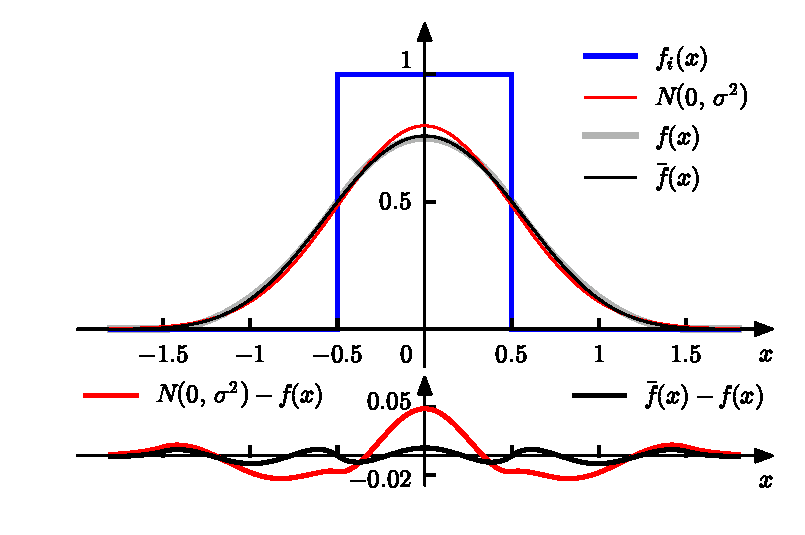
\includegraphics[width=\textwidth]{figuras/example_7_17.pdf}
  \end{minipage}\hfill
  \begin{minipage}[c]{0.25\textwidth}
    \caption{
      Corrección del error mediante la expansión Hermite. Se compara la densidad verdadera \(f(x)\) de la variable aleatoria \(\x=\x_1+\x_2+\x_2\), con \(\x_i\sim f_i(x)\) independientes, con la aproximación gaussiana dada por el teorema central del límite y la corrección \(\bar{f}(x)\).
    }\label{fig:example_7_17}
  \end{minipage}
\end{figure}

Un comentario adicional sobre este ejemplo es que el momento cuarto de \(\x\) puede calcularse empleando la función generadora de momentos. Como las variables aleatorias \(\x_i\) son i.i.d., del teorema de la convolución (ver la ecuación \ref{eq:characteristic_function_convolution_theorem}), la función generadora de momentos de \(\x=\x_1+\x_2+\x_3\) es
\[
 \Phibf(s)=\Phibf_i^3(s),
\]
donde \(\Phibf_i(s)\) es la función generadora de momentos de \(\x_i\). La función generadora de momentos de una variable aleatoria uniforme en el intervalo \((-T/2,\,T/2)\) se calculó en la sección \ref{sec:uniform_moments} y su expansión de Taylor está dada por la ecuación \ref{eq:uniform_moment_generating_function_taylor}, que con \(T=1\) es
\begin{align*}
 \Phibf_i(s)&=\sum_{k=0}^\infty\frac{1}{2^{2k}(2k+1)!}s^{2k}\\
   &=1+\frac{1}{2^2\times3!}s^2+\frac{1}{2^4\times5!}s^4+\dots\\
   &=1+\frac{1}{24}s^2+\frac{1}{1920}s^4+\dots.
\end{align*}
Combinando los resultados, la función generadora de momentos de \(\x\) es
\begin{equation}\label{eq:example_7_17_characteristic}
  \Phibf(s)=\left(1+\frac{1}{24}s^2+\frac{1}{1920}s^4+\dots\right)^3.
\end{equation}
De la ecuación \ref{eq:moments_theorem}, el momento cuarto de \(\x\) es la derivada cuarta de la función generadora de momentos evaluada en \(s=0\),
\[
 m_4=E\{\x^4\}=\Phibf^{(4)}(0).
\]
Al derivar \(n\) veces un polinomio y evaluar en cero, el único término que no se anula es el que correspondiente al grado \(n\). Al desarrollar la potencia al cubo en la ecuación \ref{eq:example_7_17_characteristic}, el término de grado 4 es
\[
  \Phibf(s)=\dots+\frac{3}{24^2}s^4+\frac{3}{1920}s^4+\dots=\dots+\frac{1}{192}s^4+\frac{3}{1920}s^4+\dots=\dots+\frac{13}{1920}s^4+\dots
\]
y al derivar cuatro veces y evaluar en cero, se obtiene que
\[
 m_4=\Phibf^{(4)}(0)=\frac{13\times4!}{1920}=\frac{13}{80}.
\]

\paragraph{Sobre la prueba del teorema central del límite} Se justificará la aproximación de la ecuación \ref{eq:central_limit_theorem_density} empleando funciones características. La demostración puede hacerse de forma muy similar a la demostración de la ley débil de los grandes números incluida en la sección \ref{sec:lln}\footnote{Ver \url{https://en.wikipedia.org/wiki/Central_limit_theorem\#Proof_of_classical_CLT}, por ejemplo.}, pero se seguirá el razonamiento realizado en \cite{papoulis2002probability}. Por simplicidad, se asumirá que \(\eta_i=0\). Denotando como \(\Phi_i(\omega)\) y \(\Phi(\omega)\) a las funciones características de las variables aleatorias \(\x_i\) y \(\x=\x_1+\dots+\x_n\) respectivamente, por la hipótesis de independencia se cumple que 
\[
 \Phi(\omega)=\Phi_1(\omega)\dots\Phi_n(\omega).
\]
Las funciones características segundas \(\Psi_i(\omega)=\ln\Phi_i(\omega)\) en torno al origen pueden aproximarse por una parábola. Efectivamente, realizando un desarrollo de Taylor en torno a cero, se tiene que
\[
 \Psi_i(\omega)=\Psi_i(0)+\frac{\Psi'_i(0)}{1!}\omega+\frac{\Psi''_i(0)}{2!}\omega^2+O(\omega^3).
\]
De la ecuación \ref{eq:characteristic_function} de la definición de la función característica se deduce que
\[
 \Phi_i(0)=1,\qquad\qquad\Phi'_i(0)=jE\{\x_i\}=j\eta_i=0,\qquad\qquad\Phi''_i(0)=-E\{\x_i^2\}=-(\eta_i^2+\sigma_i^2)=-\sigma_i^2
\]
y como
\[
\def\arraystretch{2.4}
 \begin{array}{l}
  \Psi_i(\omega)=\ln\Phi'_i(\omega)\\
  \Psi'_i(\omega)=\dfrac{\Phi'_i(\omega)}{\Phi_i(\omega)}\\
  \Psi''_i(\omega)=\dfrac{\Phi''_i(\omega)\Phi_i(\omega)-\Phi'^2_i(\omega)}{\Phi^2_i(\omega)}
 \end{array}
 \qquad\Rightarrow\qquad
 \begin{array}{l}
  \Psi_i(0)=0\\
  \Psi'_i(0)=0\\
  \Psi''_i(0)=-\sigma_i^2,
 \end{array}
\]
el desarrollo de Taylor queda
\begin{equation}\label{eq:central_limit_theorem_characteristic_taylor}
 \Psi_i(\omega)=-\frac{1}{2}\sigma_i^2\omega^2+O(\omega^3).
\end{equation}
Por lo tanto, las funciones características se pueden aproximar por 
\[
 \Phi_i(\omega)\approx e^{-\sigma_i^2\omega/2},\qquad\textrm{para }|\omega|<\epsilon,
\]
resultando en que 
\begin{equation}\label{eq:central_limit_theorem_characteristic}
 \Phi(\omega)\approx e^{-\sigma_1^2\omega/2}\dots e^{-\sigma_n^2\omega/2}=e^{-\sigma^2\omega/2}.
\end{equation}
Observar que si las variables aleatorias son continuas, se cumple que (ver la ecuación \ref{eq:characteristic_function_maximum})
\[
 \Phi_i(0)=1\qquad\qquad\textrm{y}\qquad\qquad|\Phi_i(\omega)|<1,\qquad\textrm{para }|\omega|\neq0.
\]
Esto sugiere que para \(\epsilon\) pequeño y \(n\) grande, la función \(\Phi(\omega)\) es despreciable para \(|\omega|>\epsilon\). Lo mismo ocurre con la exponencial \(e^{-\sigma^2\omega/2}\) si \(\sigma^2\to\infty\). En ese caso, la aproximación de la ecuación \ref{eq:central_limit_theorem_characteristic} es válida para todo \(\omega\), y considerando que, como indica la ecuación \ref{eq:normal_rv_characteristic_function}, se trata de la función característica de una variable aleatoria con densidad \(N(0,\,\sigma^2)\), el resultado es acorde a la aproximación del teorema central del límite dado por la ecuación \ref{eq:central_limit_theorem_density}.

La forma exacta del teorema establece que la variable aleatoria normalizada
\[
 \z=\frac{\x_1+\dots+\x_2}{\sigma},\qquad\textrm{donde }\sigma^2=\sigma_1^2+\dots+\sigma_n^2,
\]
tiende a una variable aleatoria \(N(0,\,1)\) cuando \(n\to\infty\), es decir,
\begin{equation}\label{eq:central_limit_theorem_density_normalized}
  f_z(z)\xrightarrow[n\to\infty]{}\frac{1}{\sqrt{2\pi}}e^{-z^2/2}.
\end{equation}
A continuación, se esboza una prueba bajo la hipótesis de que las variables aleatorias \(\x_i\) son i.i.d. En ese caso,
\[
 \Phi_1(\omega)=\dots=\Phi_n(\omega)\qquad\qquad\textrm{y}\qquad\qquad\sigma=\sigma_i\sqrt{n},
\]
por lo que 
\[
 \Phi_z(\omega)=\Phi_i^n\left(\frac{\omega}{\sigma_i\sqrt{n}}\right), 
\]
donde se empleó el hecho de que la función característica de la variable aleatoria \(\x_i/\sigma\) es \(\Phi_i(\omega/\sigma)\), como indica la ecuación \ref{eq:characteristic_function_of_linear_function_of_rv}. Tomando el logaritmo, se obtiene que 
\[
 \Psi_z(\omega)=n\Psi_i\left(\frac{\omega}{\sigma_i\sqrt{n}}\right).
\]
Empleando la ecuación \ref{eq:central_limit_theorem_characteristic_taylor} de la expansión de Taylor de la función característica segunda \(\Psi_i(\omega)=\ln\Phi_i(\omega)\) en torno al origen, se tiene que 
\begin{align*}
 \Psi_z(\omega)=n\Psi_i\left(\frac{\omega}{\sigma_i\sqrt{n}}\right)&=n\left\{-\dfrac{\sigma_i^2\left(\dfrac{\omega}{\sigma_i\sqrt{n}}\right)^2}{2}+O\left[\left(\dfrac{\omega}{\sigma_i\sqrt{n}}\right)^3\right]\right\}\\
   &\overset{(a)}{=}-\frac{\omega^2}{2}+O\left(\frac{\omega^3}{\sqrt{n}}\right),
\end{align*}
donde en \((a)\) se consideró que \(nO(1/n^{3/2})=O(n/n^{3/2})=O(1/\sqrt{n})\). Se concluye que
\[
 \Psi_z(\omega)=-\frac{\omega^2}{2}+O\left(\frac{\omega^3}{\sqrt{n}}\right)
 \xrightarrow[n\to\infty]{}-\frac{\omega^2}{2},
\]
lo que muestra que 
\[
 \Phi_z(\omega)\xrightarrow[n\to\infty]{}e^{-\omega^2/2},
\]
obteniendo el resultado de la ecuación \ref{eq:central_limit_theorem_density_normalized}. Observar que lo que permite concluir que se cumple la ecuación \ref{eq:central_limit_theorem_density_normalized} a partir de la convergencia de la función característica, es el teorema de continuidad de Levy, como en la demostración de la ley débil de los grandes números de la sección \ref{sec:lln}.

\chapter{Estadística}

\section{Introducción}

Probabilidad es una disciplina matemática desarrollada como un modelo abstracto y sus conclusiones son deducciones basadas en axiomas. La estadística trata con las aplicaciones de la teoría de probabilidad en problemas reales y sus conclusiones son inferencias basadas en observaciones. La conexión entre los conceptos probabilísticos y la realidad reside en la aproximación
\[
 p\approx\frac{n_A}{n},
\]
que relaciona la probabilidad \(p=P(A)\) de un evento \(A\) con el número \(n_A\) de ocurrencias de \(A\) en \(n\) ensayos del experimento físico subyacente. Esta fórmula empírica se emplea para brindar la interpretación de frecuencia relativa de todos los conceptos probabilísticos.

En una investigación estadística se trata con dos clases generales de problemas. En la primera clase, se asume que el modelo probabilístico es conocido y el objetivo es realizar predicciones vinculadas a observaciones futuras. Por ejemplo, se conoce la distribución de probabilidad \(F(x)\) de una variable aleatoria \(\x\) y se desea predecir el promedio \(\bar{x}\) de \(n\)  muestras futuras, o se conoce la probabilidad \(p\) de un evento \(A\) y se quiere predecir la cantidad de ocurrencias \(n_A\) de \(A\) en \(n\) ensayos. En ambos casos, se parte del modelo para inferir sobre las observaciones. En la segunda clase, uno o mas parámetros \(\theta_i\) del modelo son desconocidos y el objetivo es estimar sus valores (estimación de parámetros) o decidir si \(\theta_i\) es un conjunto de constantes conocidas \(\theta_{0i}\) (test de hipótesis). Por ejemplo, se observan los valores \(x_i\) de una variable aleatoria \(\x\) y se desea estimar su media \(\eta\), o decidir si aceptar la hipótesis de que \(\eta=5.3\). Una moneda es lanzada al aire 1000 veces, y se obtiene cara 465 veces. Con esta información, se quiere estimar la probabilidad \(p\) de la cara, o decidir si la moneda es justa. En ambos casos, se parte de las observaciones para realizar inferencias sobre el modelo. Este capítulo se concentra en los problemas de estimación de parámetros y test de hipótesis. Como preparación, a continuación se comenta brevemente sobre el problema de predicción.

\paragraph{Predicción} Sea una variable aleatoria \(\x\) con distribución conocida de la cual se quiere predecir su valor en un ensayo futuro. Una \emph{predicción puntual} de \(\x\) es la determinación de una constante \(c\) elegida de forma de minimizar el error \(\x-c\) en algún sentido. En un ensayo específico, \(\x\) puede tomar muchos valores, por lo que el valor que tomará no puede predecirse, solo puede estimarse. Si el criterio para la elección de \(c\) es la minimización del error MS \(E\{(\x-c)^2\}\), se cumple que \(c=E\{\x\}\), como se mostró en la sección \ref{sec:mean_square_estimation}. 

Un \emph{intervalo de predicción} de \(\x\) es la determinación de dos constantes \(c_1\) y \(c_2\) de forma de que
\begin{equation}\label{eq:statistics_interval_prediction}
  P[c_1<\x<c_2]=\gamma=1-\delta,
\end{equation}
donde \(\gamma\) es una constante dada llamada \emph{coeficiente de confianza}. Esta ecuación indica que si se predice que el valor \(x\) que tomará \(\x\) en el próximo ensayo va a estar en el intervalo \((c_1,\,c_2)\), la predicción va a ser correcta el \(100\gamma\) \% de los casos. El problema en intervalo de predicción es encontrar \(c_1\) y \(c_2\) de forma de minimizar la diferencia \(c_2-c_1\) sujeta a la restricción dada por la ecuación \ref{eq:statistics_interval_prediction}. La elección de \(\gamma\) se rige por dos requerimientos en conflicto. Si \(\gamma\) es cercano a 1, la predicción de que \(x\) estará en el intervalo \((c_1,\,c_2)\) es confiable, pero la diferencia \(c_2-c_1\) es grande y brinda poca información sobre \(x\). Si se reduce \(\gamma\), se reduce \(c_2-c_1\), pero la estimación es menos confiable. Se mostrará a continuación que si la densidad de probabilidad \(f(x)\) de \(\x\) es unimodal, \(c_2-c_1\) es mínimo para un \(\gamma\) dado si \(f(c_1)=f(c_2)\) (teorema 9.3.2 en \cite{casella2001statistical}):
\begin{itemize}
 \item[] \emph{Teorema:} Sea \(f(x)\) una densidad unimodal. Si el intervalo \((c_1,\,c_2)\) satisface que 
 \begin{enumerate}
  \item \(\displaystyle P[c_1<\x<c_2]=\int_{c_1}^{c_2}f(x)\,dx=\gamma\),
  \item \(f(c_1)=f(c_2)>0\), y
  \item \(c_1\leq x^*\leq c_2\), donde \(x^*\) es la moda de \(f(x)\) (ubicación del máximo),
 \end{enumerate}
 \item[] el intervalo \((c_1,\,c_2)\) es el mas corto entre todos los intervalos que cumplen 1.
 \item[] \emph{Demostración:} Sea \((c'_1,\,c'_2)\) cualquier intervalo tal que \(c'_2-c'_1<c_2-c_1\). Se demostrará que esto implica que
 \[
  P[c'_1<\x<c'_2]=\int_{c'_1}^{c'_2}f(x)\,dx<\gamma.
 \]
 El caso en que \((c'_1,\,c'_2)\subset(c_1,\,c_2)\) es trivial, ya que inmediatamente se observa que se cumple que
 \[
  \int_{c'_1}^{c'_2}f(x)\,dx<\int_{c_1}^{c_2}f(x)\,dx=\gamma.
 \]
 La prueba se realizará únicamente para el caso en que \(c'_1\leq c_1\), dado que la prueba para el caso en que \(c'_1>c_1\) es análoga. Asumiendo entonces que \(c'_1\leq c_1\), hay que distinguir dos casos, \(c'_2\leq c_1\) y \(c'_2>c_1\).
 \begin{itemize}
  \item Caso \(c'_2\leq c_1\): se cumple que \(c'_1\leq c'_2\leq c_1\leq x^*\). Por lo tanto,
  \[
   \int_{c'_1}^{c'_2}f(x)\,dx\overset{(a)}{\leq} f(c'_2)(c'_2-c'_1)
     \overset{(b)}{\leq}f(c_1)(c'_2-c'_1)
     \overset{(c)}{<}f(c_1)(c_2-c_1)
     \overset{(d)}{\leq}\int_{c_1}^{c_2}f(x)\,dx=\gamma,
  \]
  donde en \((a)\) se empleó que como \(x\leq c'_2\leq x^*\), \(f(x)\leq f(c'_2)\) para todo \(x\in(c'_1,\,c'_2)\), en \((b)\) se empleó que \(c'_2\leq c_1\leq x^*\) y por lo tanto, \(f(c'_2)\leq f(c_1)\), en \((c)\) se tuvo en cuenta que \(c'_2-c'_1<c_2-c_1\) y \(f(c_1)>0\) y en \((d)\) se consideró que por 2., 3. y la unimodalidad, \(f(x)\geq f(c_1)\) para todo \(x\in(c_1,\,c_2)\), completando la prueba para este caso.
  \item Caso \(c'_2>c_1\): se cumple que \(c'_1\leq c_1<c'_2<c_2\). No puede ocurrir que \(c'_2\geq c_2\) por la condición de que \(c'_2-c'_1>c_2-c_1\). En este caso, se tiene que 
  \begin{align*}
   \int_{c'_1}^{c'_2}f(x)\,dx&=\int_{c_1}^{c_2}f(x)\,dx+\left[\int_{c'_1}^{c_1}f(x)\,dx-\int_{c'_2}^{c_2}f(x)\,dx\right]\\
    &=\gamma+\left[\int_{c'_1}^{c_1}f(x)\,dx-\int_{c'_2}^{c_2}f(x)\,dx\right],
  \end{align*}
  por lo que la demostración del teorema se completa demostrando que el término entre paréntesis rectos es negativo. Considerando 3., la unimodalidad y el orden \(c'_1\leq c_1<c'_2<c_2\), se deduce que
  \[
   \int_{c'_1}^{c_1}f(x)\,dx\leq f(c_1)(c_1-c'_1)
   \qquad\textrm{y}\qquad
   \int_{c'_2}^{c_2}f(x)\,dx\geq f(c_2)(c_2-c'_2),
  \]
  y por lo tanto,
  \begin{align*}
   \int_{c'_1}^{c_1}f(x)\,dx-\int_{c'_2}^{c_2}f(x)\,dx&\leq f(c_1)(c_1-c'_1)-f(c_2)(c_2-c'_2)\\
    &\overset{(a)}{\leq} f(c_1)\left[(c_1-c'_1)-(c_2-c'_2)\right]\\
    &=f(c_1)\left[(c'_2-c'_1)-(c_2-c_1)\right]\\
    &\overset{(b)}{<}0,
  \end{align*}
  donde en \(a\) se tuvo en cuenta 2. y en \((b)\) que \(c'_2-c'_1<c_2-c_1\) y \(f(c_1)\), concluyendo la prueba.  
 \end{itemize}
\end{itemize}



\bibliographystyle{ieeetr}
\bibliography{papoulis_probability_notes}

\end{document}
